\documentclass[tikz]{standalone}
\usepackage{graphicx}
\usepackage{tikz}
\usetikzlibrary{shapes}
\usetikzlibrary{positioning}
\usetikzlibrary{patterns}
\usepackage{pgfplots}
%\providecommand{\mathdefault}[1]{}
\usepackage{pdflscape} % makes pages landscape
%\usepackage[labelfont={bf}]{caption}
\usepackage{siunitx}
\sisetup{detect-weight=true, detect-family=true} % makes siunitx follow font formatting like bold, italic, etc.

\usepackage{newpxtext,newpxmath}

\begin{document}

\begin{tikzpicture}

    \node[inner sep=0pt] (geom label) at (0,0) {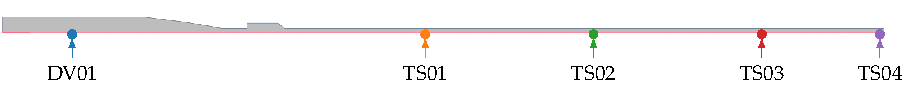
\includegraphics[width=5.75in]{../figures/STAR_new_geometry_colorlabels_tikz.pdf}};
    \node[inner sep=0pt] (plot) at (0,-6){%% Creator: Matplotlib, PGF backend
%%
%% To include the figure in your LaTeX document, write
%%   \input{<filename>.pgf}
%%
%% Make sure the required packages are loaded in your preamble
%%   \usepackage{pgf}
%%
%% Also ensure that all the required font packages are loaded; for instance,
%% the lmodern package is sometimes necessary when using math font.
%%   \usepackage{lmodern}
%%
%% Figures using additional raster images can only be included by \input if
%% they are in the same directory as the main LaTeX file. For loading figures
%% from other directories you can use the `import` package
%%   \usepackage{import}
%%
%% and then include the figures with
%%   \import{<path to file>}{<filename>.pgf}
%%
%% Matplotlib used the following preamble
%%   \def\mathdefault#1{#1}
%%   \everymath=\expandafter{\the\everymath\displaystyle}
%%   \usepackage[utf8]{inputenc}
%%   \usepackage[T1]{fontenc}
%%   \usepackage[detect-all]{siunitx}
%%   \providecommand{\mathdefault}[1]{}
%%   \makeatletter\@ifpackageloaded{underscore}{}{\usepackage[strings]{underscore}}\makeatother
%%
\begingroup%
\makeatletter%
\begin{pgfpicture}%
\pgfpathrectangle{\pgfpointorigin}{\pgfqpoint{5.750000in}{4.312500in}}%
\pgfusepath{use as bounding box, clip}%
\begin{pgfscope}%
\pgfsetbuttcap%
\pgfsetmiterjoin%
\pgfsetlinewidth{0.000000pt}%
\definecolor{currentstroke}{rgb}{0.000000,0.000000,0.000000}%
\pgfsetstrokecolor{currentstroke}%
\pgfsetstrokeopacity{0.000000}%
\pgfsetdash{}{0pt}%
\pgfpathmoveto{\pgfqpoint{0.000000in}{0.000000in}}%
\pgfpathlineto{\pgfqpoint{5.750000in}{0.000000in}}%
\pgfpathlineto{\pgfqpoint{5.750000in}{4.312500in}}%
\pgfpathlineto{\pgfqpoint{0.000000in}{4.312500in}}%
\pgfpathlineto{\pgfqpoint{0.000000in}{0.000000in}}%
\pgfpathclose%
\pgfusepath{}%
\end{pgfscope}%
\begin{pgfscope}%
\pgfsetbuttcap%
\pgfsetmiterjoin%
\pgfsetlinewidth{0.000000pt}%
\definecolor{currentstroke}{rgb}{0.000000,0.000000,0.000000}%
\pgfsetstrokecolor{currentstroke}%
\pgfsetstrokeopacity{0.000000}%
\pgfsetdash{}{0pt}%
\pgfpathmoveto{\pgfqpoint{0.654407in}{0.580216in}}%
\pgfpathlineto{\pgfqpoint{5.585000in}{0.580216in}}%
\pgfpathlineto{\pgfqpoint{5.585000in}{4.111140in}}%
\pgfpathlineto{\pgfqpoint{0.654407in}{4.111140in}}%
\pgfpathlineto{\pgfqpoint{0.654407in}{0.580216in}}%
\pgfpathclose%
\pgfusepath{}%
\end{pgfscope}%
\begin{pgfscope}%
\pgfpathrectangle{\pgfqpoint{0.654407in}{0.580216in}}{\pgfqpoint{4.930593in}{3.530924in}}%
\pgfusepath{clip}%
\pgfsetrectcap%
\pgfsetroundjoin%
\pgfsetlinewidth{0.803000pt}%
\definecolor{currentstroke}{rgb}{0.690196,0.690196,0.690196}%
\pgfsetstrokecolor{currentstroke}%
\pgfsetdash{}{0pt}%
\pgfpathmoveto{\pgfqpoint{0.878483in}{0.580216in}}%
\pgfpathlineto{\pgfqpoint{0.878483in}{4.111140in}}%
\pgfusepath{stroke}%
\end{pgfscope}%
\begin{pgfscope}%
\pgfsetbuttcap%
\pgfsetroundjoin%
\definecolor{currentfill}{rgb}{0.000000,0.000000,0.000000}%
\pgfsetfillcolor{currentfill}%
\pgfsetlinewidth{0.803000pt}%
\definecolor{currentstroke}{rgb}{0.000000,0.000000,0.000000}%
\pgfsetstrokecolor{currentstroke}%
\pgfsetdash{}{0pt}%
\pgfsys@defobject{currentmarker}{\pgfqpoint{0.000000in}{-0.048611in}}{\pgfqpoint{0.000000in}{0.000000in}}{%
\pgfpathmoveto{\pgfqpoint{0.000000in}{0.000000in}}%
\pgfpathlineto{\pgfqpoint{0.000000in}{-0.048611in}}%
\pgfusepath{stroke,fill}%
}%
\begin{pgfscope}%
\pgfsys@transformshift{0.878483in}{0.580216in}%
\pgfsys@useobject{currentmarker}{}%
\end{pgfscope}%
\end{pgfscope}%
\begin{pgfscope}%
\definecolor{textcolor}{rgb}{0.000000,0.000000,0.000000}%
\pgfsetstrokecolor{textcolor}%
\pgfsetfillcolor{textcolor}%
\pgftext[x=0.878483in,y=0.482994in,,top]{\color{textcolor}{\rmfamily\fontsize{9.000000}{10.800000}\selectfont\catcode`\^=\active\def^{\ifmmode\sp\else\^{}\fi}\catcode`\%=\active\def%{\%}$\mathdefault{0.000}$}}%
\end{pgfscope}%
\begin{pgfscope}%
\pgfpathrectangle{\pgfqpoint{0.654407in}{0.580216in}}{\pgfqpoint{4.930593in}{3.530924in}}%
\pgfusepath{clip}%
\pgfsetrectcap%
\pgfsetroundjoin%
\pgfsetlinewidth{0.803000pt}%
\definecolor{currentstroke}{rgb}{0.690196,0.690196,0.690196}%
\pgfsetstrokecolor{currentstroke}%
\pgfsetdash{}{0pt}%
\pgfpathmoveto{\pgfqpoint{1.704192in}{0.580216in}}%
\pgfpathlineto{\pgfqpoint{1.704192in}{4.111140in}}%
\pgfusepath{stroke}%
\end{pgfscope}%
\begin{pgfscope}%
\pgfsetbuttcap%
\pgfsetroundjoin%
\definecolor{currentfill}{rgb}{0.000000,0.000000,0.000000}%
\pgfsetfillcolor{currentfill}%
\pgfsetlinewidth{0.803000pt}%
\definecolor{currentstroke}{rgb}{0.000000,0.000000,0.000000}%
\pgfsetstrokecolor{currentstroke}%
\pgfsetdash{}{0pt}%
\pgfsys@defobject{currentmarker}{\pgfqpoint{0.000000in}{-0.048611in}}{\pgfqpoint{0.000000in}{0.000000in}}{%
\pgfpathmoveto{\pgfqpoint{0.000000in}{0.000000in}}%
\pgfpathlineto{\pgfqpoint{0.000000in}{-0.048611in}}%
\pgfusepath{stroke,fill}%
}%
\begin{pgfscope}%
\pgfsys@transformshift{1.704192in}{0.580216in}%
\pgfsys@useobject{currentmarker}{}%
\end{pgfscope}%
\end{pgfscope}%
\begin{pgfscope}%
\definecolor{textcolor}{rgb}{0.000000,0.000000,0.000000}%
\pgfsetstrokecolor{textcolor}%
\pgfsetfillcolor{textcolor}%
\pgftext[x=1.704192in,y=0.482994in,,top]{\color{textcolor}{\rmfamily\fontsize{9.000000}{10.800000}\selectfont\catcode`\^=\active\def^{\ifmmode\sp\else\^{}\fi}\catcode`\%=\active\def%{\%}$\mathdefault{0.001}$}}%
\end{pgfscope}%
\begin{pgfscope}%
\pgfpathrectangle{\pgfqpoint{0.654407in}{0.580216in}}{\pgfqpoint{4.930593in}{3.530924in}}%
\pgfusepath{clip}%
\pgfsetrectcap%
\pgfsetroundjoin%
\pgfsetlinewidth{0.803000pt}%
\definecolor{currentstroke}{rgb}{0.690196,0.690196,0.690196}%
\pgfsetstrokecolor{currentstroke}%
\pgfsetdash{}{0pt}%
\pgfpathmoveto{\pgfqpoint{2.529900in}{0.580216in}}%
\pgfpathlineto{\pgfqpoint{2.529900in}{4.111140in}}%
\pgfusepath{stroke}%
\end{pgfscope}%
\begin{pgfscope}%
\pgfsetbuttcap%
\pgfsetroundjoin%
\definecolor{currentfill}{rgb}{0.000000,0.000000,0.000000}%
\pgfsetfillcolor{currentfill}%
\pgfsetlinewidth{0.803000pt}%
\definecolor{currentstroke}{rgb}{0.000000,0.000000,0.000000}%
\pgfsetstrokecolor{currentstroke}%
\pgfsetdash{}{0pt}%
\pgfsys@defobject{currentmarker}{\pgfqpoint{0.000000in}{-0.048611in}}{\pgfqpoint{0.000000in}{0.000000in}}{%
\pgfpathmoveto{\pgfqpoint{0.000000in}{0.000000in}}%
\pgfpathlineto{\pgfqpoint{0.000000in}{-0.048611in}}%
\pgfusepath{stroke,fill}%
}%
\begin{pgfscope}%
\pgfsys@transformshift{2.529900in}{0.580216in}%
\pgfsys@useobject{currentmarker}{}%
\end{pgfscope}%
\end{pgfscope}%
\begin{pgfscope}%
\definecolor{textcolor}{rgb}{0.000000,0.000000,0.000000}%
\pgfsetstrokecolor{textcolor}%
\pgfsetfillcolor{textcolor}%
\pgftext[x=2.529900in,y=0.482994in,,top]{\color{textcolor}{\rmfamily\fontsize{9.000000}{10.800000}\selectfont\catcode`\^=\active\def^{\ifmmode\sp\else\^{}\fi}\catcode`\%=\active\def%{\%}$\mathdefault{0.002}$}}%
\end{pgfscope}%
\begin{pgfscope}%
\pgfpathrectangle{\pgfqpoint{0.654407in}{0.580216in}}{\pgfqpoint{4.930593in}{3.530924in}}%
\pgfusepath{clip}%
\pgfsetrectcap%
\pgfsetroundjoin%
\pgfsetlinewidth{0.803000pt}%
\definecolor{currentstroke}{rgb}{0.690196,0.690196,0.690196}%
\pgfsetstrokecolor{currentstroke}%
\pgfsetdash{}{0pt}%
\pgfpathmoveto{\pgfqpoint{3.355608in}{0.580216in}}%
\pgfpathlineto{\pgfqpoint{3.355608in}{4.111140in}}%
\pgfusepath{stroke}%
\end{pgfscope}%
\begin{pgfscope}%
\pgfsetbuttcap%
\pgfsetroundjoin%
\definecolor{currentfill}{rgb}{0.000000,0.000000,0.000000}%
\pgfsetfillcolor{currentfill}%
\pgfsetlinewidth{0.803000pt}%
\definecolor{currentstroke}{rgb}{0.000000,0.000000,0.000000}%
\pgfsetstrokecolor{currentstroke}%
\pgfsetdash{}{0pt}%
\pgfsys@defobject{currentmarker}{\pgfqpoint{0.000000in}{-0.048611in}}{\pgfqpoint{0.000000in}{0.000000in}}{%
\pgfpathmoveto{\pgfqpoint{0.000000in}{0.000000in}}%
\pgfpathlineto{\pgfqpoint{0.000000in}{-0.048611in}}%
\pgfusepath{stroke,fill}%
}%
\begin{pgfscope}%
\pgfsys@transformshift{3.355608in}{0.580216in}%
\pgfsys@useobject{currentmarker}{}%
\end{pgfscope}%
\end{pgfscope}%
\begin{pgfscope}%
\definecolor{textcolor}{rgb}{0.000000,0.000000,0.000000}%
\pgfsetstrokecolor{textcolor}%
\pgfsetfillcolor{textcolor}%
\pgftext[x=3.355608in,y=0.482994in,,top]{\color{textcolor}{\rmfamily\fontsize{9.000000}{10.800000}\selectfont\catcode`\^=\active\def^{\ifmmode\sp\else\^{}\fi}\catcode`\%=\active\def%{\%}$\mathdefault{0.003}$}}%
\end{pgfscope}%
\begin{pgfscope}%
\pgfpathrectangle{\pgfqpoint{0.654407in}{0.580216in}}{\pgfqpoint{4.930593in}{3.530924in}}%
\pgfusepath{clip}%
\pgfsetrectcap%
\pgfsetroundjoin%
\pgfsetlinewidth{0.803000pt}%
\definecolor{currentstroke}{rgb}{0.690196,0.690196,0.690196}%
\pgfsetstrokecolor{currentstroke}%
\pgfsetdash{}{0pt}%
\pgfpathmoveto{\pgfqpoint{4.181317in}{0.580216in}}%
\pgfpathlineto{\pgfqpoint{4.181317in}{4.111140in}}%
\pgfusepath{stroke}%
\end{pgfscope}%
\begin{pgfscope}%
\pgfsetbuttcap%
\pgfsetroundjoin%
\definecolor{currentfill}{rgb}{0.000000,0.000000,0.000000}%
\pgfsetfillcolor{currentfill}%
\pgfsetlinewidth{0.803000pt}%
\definecolor{currentstroke}{rgb}{0.000000,0.000000,0.000000}%
\pgfsetstrokecolor{currentstroke}%
\pgfsetdash{}{0pt}%
\pgfsys@defobject{currentmarker}{\pgfqpoint{0.000000in}{-0.048611in}}{\pgfqpoint{0.000000in}{0.000000in}}{%
\pgfpathmoveto{\pgfqpoint{0.000000in}{0.000000in}}%
\pgfpathlineto{\pgfqpoint{0.000000in}{-0.048611in}}%
\pgfusepath{stroke,fill}%
}%
\begin{pgfscope}%
\pgfsys@transformshift{4.181317in}{0.580216in}%
\pgfsys@useobject{currentmarker}{}%
\end{pgfscope}%
\end{pgfscope}%
\begin{pgfscope}%
\definecolor{textcolor}{rgb}{0.000000,0.000000,0.000000}%
\pgfsetstrokecolor{textcolor}%
\pgfsetfillcolor{textcolor}%
\pgftext[x=4.181317in,y=0.482994in,,top]{\color{textcolor}{\rmfamily\fontsize{9.000000}{10.800000}\selectfont\catcode`\^=\active\def^{\ifmmode\sp\else\^{}\fi}\catcode`\%=\active\def%{\%}$\mathdefault{0.004}$}}%
\end{pgfscope}%
\begin{pgfscope}%
\pgfpathrectangle{\pgfqpoint{0.654407in}{0.580216in}}{\pgfqpoint{4.930593in}{3.530924in}}%
\pgfusepath{clip}%
\pgfsetrectcap%
\pgfsetroundjoin%
\pgfsetlinewidth{0.803000pt}%
\definecolor{currentstroke}{rgb}{0.690196,0.690196,0.690196}%
\pgfsetstrokecolor{currentstroke}%
\pgfsetdash{}{0pt}%
\pgfpathmoveto{\pgfqpoint{5.007025in}{0.580216in}}%
\pgfpathlineto{\pgfqpoint{5.007025in}{4.111140in}}%
\pgfusepath{stroke}%
\end{pgfscope}%
\begin{pgfscope}%
\pgfsetbuttcap%
\pgfsetroundjoin%
\definecolor{currentfill}{rgb}{0.000000,0.000000,0.000000}%
\pgfsetfillcolor{currentfill}%
\pgfsetlinewidth{0.803000pt}%
\definecolor{currentstroke}{rgb}{0.000000,0.000000,0.000000}%
\pgfsetstrokecolor{currentstroke}%
\pgfsetdash{}{0pt}%
\pgfsys@defobject{currentmarker}{\pgfqpoint{0.000000in}{-0.048611in}}{\pgfqpoint{0.000000in}{0.000000in}}{%
\pgfpathmoveto{\pgfqpoint{0.000000in}{0.000000in}}%
\pgfpathlineto{\pgfqpoint{0.000000in}{-0.048611in}}%
\pgfusepath{stroke,fill}%
}%
\begin{pgfscope}%
\pgfsys@transformshift{5.007025in}{0.580216in}%
\pgfsys@useobject{currentmarker}{}%
\end{pgfscope}%
\end{pgfscope}%
\begin{pgfscope}%
\definecolor{textcolor}{rgb}{0.000000,0.000000,0.000000}%
\pgfsetstrokecolor{textcolor}%
\pgfsetfillcolor{textcolor}%
\pgftext[x=5.007025in,y=0.482994in,,top]{\color{textcolor}{\rmfamily\fontsize{9.000000}{10.800000}\selectfont\catcode`\^=\active\def^{\ifmmode\sp\else\^{}\fi}\catcode`\%=\active\def%{\%}$\mathdefault{0.005}$}}%
\end{pgfscope}%
\begin{pgfscope}%
\definecolor{textcolor}{rgb}{0.000000,0.000000,0.000000}%
\pgfsetstrokecolor{textcolor}%
\pgfsetfillcolor{textcolor}%
\pgftext[x=3.119703in,y=0.317048in,,top]{\color{textcolor}{\rmfamily\fontsize{11.000000}{13.200000}\selectfont\catcode`\^=\active\def^{\ifmmode\sp\else\^{}\fi}\catcode`\%=\active\def%{\%}Time (\si{\second})}}%
\end{pgfscope}%
\begin{pgfscope}%
\pgfpathrectangle{\pgfqpoint{0.654407in}{0.580216in}}{\pgfqpoint{4.930593in}{3.530924in}}%
\pgfusepath{clip}%
\pgfsetrectcap%
\pgfsetroundjoin%
\pgfsetlinewidth{0.803000pt}%
\definecolor{currentstroke}{rgb}{0.690196,0.690196,0.690196}%
\pgfsetstrokecolor{currentstroke}%
\pgfsetdash{}{0pt}%
\pgfpathmoveto{\pgfqpoint{0.654407in}{0.739341in}}%
\pgfpathlineto{\pgfqpoint{5.585000in}{0.739341in}}%
\pgfusepath{stroke}%
\end{pgfscope}%
\begin{pgfscope}%
\pgfsetbuttcap%
\pgfsetroundjoin%
\definecolor{currentfill}{rgb}{0.000000,0.000000,0.000000}%
\pgfsetfillcolor{currentfill}%
\pgfsetlinewidth{0.803000pt}%
\definecolor{currentstroke}{rgb}{0.000000,0.000000,0.000000}%
\pgfsetstrokecolor{currentstroke}%
\pgfsetdash{}{0pt}%
\pgfsys@defobject{currentmarker}{\pgfqpoint{-0.048611in}{0.000000in}}{\pgfqpoint{-0.000000in}{0.000000in}}{%
\pgfpathmoveto{\pgfqpoint{-0.000000in}{0.000000in}}%
\pgfpathlineto{\pgfqpoint{-0.048611in}{0.000000in}}%
\pgfusepath{stroke,fill}%
}%
\begin{pgfscope}%
\pgfsys@transformshift{0.654407in}{0.739341in}%
\pgfsys@useobject{currentmarker}{}%
\end{pgfscope}%
\end{pgfscope}%
\begin{pgfscope}%
\definecolor{textcolor}{rgb}{0.000000,0.000000,0.000000}%
\pgfsetstrokecolor{textcolor}%
\pgfsetfillcolor{textcolor}%
\pgftext[x=0.393027in, y=0.696296in, left, base]{\color{textcolor}{\rmfamily\fontsize{9.000000}{10.800000}\selectfont\catcode`\^=\active\def^{\ifmmode\sp\else\^{}\fi}\catcode`\%=\active\def%{\%}$\mathdefault{0.0}$}}%
\end{pgfscope}%
\begin{pgfscope}%
\pgfpathrectangle{\pgfqpoint{0.654407in}{0.580216in}}{\pgfqpoint{4.930593in}{3.530924in}}%
\pgfusepath{clip}%
\pgfsetrectcap%
\pgfsetroundjoin%
\pgfsetlinewidth{0.803000pt}%
\definecolor{currentstroke}{rgb}{0.690196,0.690196,0.690196}%
\pgfsetstrokecolor{currentstroke}%
\pgfsetdash{}{0pt}%
\pgfpathmoveto{\pgfqpoint{0.654407in}{1.412279in}}%
\pgfpathlineto{\pgfqpoint{5.585000in}{1.412279in}}%
\pgfusepath{stroke}%
\end{pgfscope}%
\begin{pgfscope}%
\pgfsetbuttcap%
\pgfsetroundjoin%
\definecolor{currentfill}{rgb}{0.000000,0.000000,0.000000}%
\pgfsetfillcolor{currentfill}%
\pgfsetlinewidth{0.803000pt}%
\definecolor{currentstroke}{rgb}{0.000000,0.000000,0.000000}%
\pgfsetstrokecolor{currentstroke}%
\pgfsetdash{}{0pt}%
\pgfsys@defobject{currentmarker}{\pgfqpoint{-0.048611in}{0.000000in}}{\pgfqpoint{-0.000000in}{0.000000in}}{%
\pgfpathmoveto{\pgfqpoint{-0.000000in}{0.000000in}}%
\pgfpathlineto{\pgfqpoint{-0.048611in}{0.000000in}}%
\pgfusepath{stroke,fill}%
}%
\begin{pgfscope}%
\pgfsys@transformshift{0.654407in}{1.412279in}%
\pgfsys@useobject{currentmarker}{}%
\end{pgfscope}%
\end{pgfscope}%
\begin{pgfscope}%
\definecolor{textcolor}{rgb}{0.000000,0.000000,0.000000}%
\pgfsetstrokecolor{textcolor}%
\pgfsetfillcolor{textcolor}%
\pgftext[x=0.393027in, y=1.369234in, left, base]{\color{textcolor}{\rmfamily\fontsize{9.000000}{10.800000}\selectfont\catcode`\^=\active\def^{\ifmmode\sp\else\^{}\fi}\catcode`\%=\active\def%{\%}$\mathdefault{0.5}$}}%
\end{pgfscope}%
\begin{pgfscope}%
\pgfpathrectangle{\pgfqpoint{0.654407in}{0.580216in}}{\pgfqpoint{4.930593in}{3.530924in}}%
\pgfusepath{clip}%
\pgfsetrectcap%
\pgfsetroundjoin%
\pgfsetlinewidth{0.803000pt}%
\definecolor{currentstroke}{rgb}{0.690196,0.690196,0.690196}%
\pgfsetstrokecolor{currentstroke}%
\pgfsetdash{}{0pt}%
\pgfpathmoveto{\pgfqpoint{0.654407in}{2.085217in}}%
\pgfpathlineto{\pgfqpoint{5.585000in}{2.085217in}}%
\pgfusepath{stroke}%
\end{pgfscope}%
\begin{pgfscope}%
\pgfsetbuttcap%
\pgfsetroundjoin%
\definecolor{currentfill}{rgb}{0.000000,0.000000,0.000000}%
\pgfsetfillcolor{currentfill}%
\pgfsetlinewidth{0.803000pt}%
\definecolor{currentstroke}{rgb}{0.000000,0.000000,0.000000}%
\pgfsetstrokecolor{currentstroke}%
\pgfsetdash{}{0pt}%
\pgfsys@defobject{currentmarker}{\pgfqpoint{-0.048611in}{0.000000in}}{\pgfqpoint{-0.000000in}{0.000000in}}{%
\pgfpathmoveto{\pgfqpoint{-0.000000in}{0.000000in}}%
\pgfpathlineto{\pgfqpoint{-0.048611in}{0.000000in}}%
\pgfusepath{stroke,fill}%
}%
\begin{pgfscope}%
\pgfsys@transformshift{0.654407in}{2.085217in}%
\pgfsys@useobject{currentmarker}{}%
\end{pgfscope}%
\end{pgfscope}%
\begin{pgfscope}%
\definecolor{textcolor}{rgb}{0.000000,0.000000,0.000000}%
\pgfsetstrokecolor{textcolor}%
\pgfsetfillcolor{textcolor}%
\pgftext[x=0.393027in, y=2.042172in, left, base]{\color{textcolor}{\rmfamily\fontsize{9.000000}{10.800000}\selectfont\catcode`\^=\active\def^{\ifmmode\sp\else\^{}\fi}\catcode`\%=\active\def%{\%}$\mathdefault{1.0}$}}%
\end{pgfscope}%
\begin{pgfscope}%
\pgfpathrectangle{\pgfqpoint{0.654407in}{0.580216in}}{\pgfqpoint{4.930593in}{3.530924in}}%
\pgfusepath{clip}%
\pgfsetrectcap%
\pgfsetroundjoin%
\pgfsetlinewidth{0.803000pt}%
\definecolor{currentstroke}{rgb}{0.690196,0.690196,0.690196}%
\pgfsetstrokecolor{currentstroke}%
\pgfsetdash{}{0pt}%
\pgfpathmoveto{\pgfqpoint{0.654407in}{2.758155in}}%
\pgfpathlineto{\pgfqpoint{5.585000in}{2.758155in}}%
\pgfusepath{stroke}%
\end{pgfscope}%
\begin{pgfscope}%
\pgfsetbuttcap%
\pgfsetroundjoin%
\definecolor{currentfill}{rgb}{0.000000,0.000000,0.000000}%
\pgfsetfillcolor{currentfill}%
\pgfsetlinewidth{0.803000pt}%
\definecolor{currentstroke}{rgb}{0.000000,0.000000,0.000000}%
\pgfsetstrokecolor{currentstroke}%
\pgfsetdash{}{0pt}%
\pgfsys@defobject{currentmarker}{\pgfqpoint{-0.048611in}{0.000000in}}{\pgfqpoint{-0.000000in}{0.000000in}}{%
\pgfpathmoveto{\pgfqpoint{-0.000000in}{0.000000in}}%
\pgfpathlineto{\pgfqpoint{-0.048611in}{0.000000in}}%
\pgfusepath{stroke,fill}%
}%
\begin{pgfscope}%
\pgfsys@transformshift{0.654407in}{2.758155in}%
\pgfsys@useobject{currentmarker}{}%
\end{pgfscope}%
\end{pgfscope}%
\begin{pgfscope}%
\definecolor{textcolor}{rgb}{0.000000,0.000000,0.000000}%
\pgfsetstrokecolor{textcolor}%
\pgfsetfillcolor{textcolor}%
\pgftext[x=0.393027in, y=2.715110in, left, base]{\color{textcolor}{\rmfamily\fontsize{9.000000}{10.800000}\selectfont\catcode`\^=\active\def^{\ifmmode\sp\else\^{}\fi}\catcode`\%=\active\def%{\%}$\mathdefault{1.5}$}}%
\end{pgfscope}%
\begin{pgfscope}%
\pgfpathrectangle{\pgfqpoint{0.654407in}{0.580216in}}{\pgfqpoint{4.930593in}{3.530924in}}%
\pgfusepath{clip}%
\pgfsetrectcap%
\pgfsetroundjoin%
\pgfsetlinewidth{0.803000pt}%
\definecolor{currentstroke}{rgb}{0.690196,0.690196,0.690196}%
\pgfsetstrokecolor{currentstroke}%
\pgfsetdash{}{0pt}%
\pgfpathmoveto{\pgfqpoint{0.654407in}{3.431093in}}%
\pgfpathlineto{\pgfqpoint{5.585000in}{3.431093in}}%
\pgfusepath{stroke}%
\end{pgfscope}%
\begin{pgfscope}%
\pgfsetbuttcap%
\pgfsetroundjoin%
\definecolor{currentfill}{rgb}{0.000000,0.000000,0.000000}%
\pgfsetfillcolor{currentfill}%
\pgfsetlinewidth{0.803000pt}%
\definecolor{currentstroke}{rgb}{0.000000,0.000000,0.000000}%
\pgfsetstrokecolor{currentstroke}%
\pgfsetdash{}{0pt}%
\pgfsys@defobject{currentmarker}{\pgfqpoint{-0.048611in}{0.000000in}}{\pgfqpoint{-0.000000in}{0.000000in}}{%
\pgfpathmoveto{\pgfqpoint{-0.000000in}{0.000000in}}%
\pgfpathlineto{\pgfqpoint{-0.048611in}{0.000000in}}%
\pgfusepath{stroke,fill}%
}%
\begin{pgfscope}%
\pgfsys@transformshift{0.654407in}{3.431093in}%
\pgfsys@useobject{currentmarker}{}%
\end{pgfscope}%
\end{pgfscope}%
\begin{pgfscope}%
\definecolor{textcolor}{rgb}{0.000000,0.000000,0.000000}%
\pgfsetstrokecolor{textcolor}%
\pgfsetfillcolor{textcolor}%
\pgftext[x=0.393027in, y=3.388048in, left, base]{\color{textcolor}{\rmfamily\fontsize{9.000000}{10.800000}\selectfont\catcode`\^=\active\def^{\ifmmode\sp\else\^{}\fi}\catcode`\%=\active\def%{\%}$\mathdefault{2.0}$}}%
\end{pgfscope}%
\begin{pgfscope}%
\pgfpathrectangle{\pgfqpoint{0.654407in}{0.580216in}}{\pgfqpoint{4.930593in}{3.530924in}}%
\pgfusepath{clip}%
\pgfsetrectcap%
\pgfsetroundjoin%
\pgfsetlinewidth{0.803000pt}%
\definecolor{currentstroke}{rgb}{0.690196,0.690196,0.690196}%
\pgfsetstrokecolor{currentstroke}%
\pgfsetdash{}{0pt}%
\pgfpathmoveto{\pgfqpoint{0.654407in}{4.104032in}}%
\pgfpathlineto{\pgfqpoint{5.585000in}{4.104032in}}%
\pgfusepath{stroke}%
\end{pgfscope}%
\begin{pgfscope}%
\pgfsetbuttcap%
\pgfsetroundjoin%
\definecolor{currentfill}{rgb}{0.000000,0.000000,0.000000}%
\pgfsetfillcolor{currentfill}%
\pgfsetlinewidth{0.803000pt}%
\definecolor{currentstroke}{rgb}{0.000000,0.000000,0.000000}%
\pgfsetstrokecolor{currentstroke}%
\pgfsetdash{}{0pt}%
\pgfsys@defobject{currentmarker}{\pgfqpoint{-0.048611in}{0.000000in}}{\pgfqpoint{-0.000000in}{0.000000in}}{%
\pgfpathmoveto{\pgfqpoint{-0.000000in}{0.000000in}}%
\pgfpathlineto{\pgfqpoint{-0.048611in}{0.000000in}}%
\pgfusepath{stroke,fill}%
}%
\begin{pgfscope}%
\pgfsys@transformshift{0.654407in}{4.104032in}%
\pgfsys@useobject{currentmarker}{}%
\end{pgfscope}%
\end{pgfscope}%
\begin{pgfscope}%
\definecolor{textcolor}{rgb}{0.000000,0.000000,0.000000}%
\pgfsetstrokecolor{textcolor}%
\pgfsetfillcolor{textcolor}%
\pgftext[x=0.393027in, y=4.060986in, left, base]{\color{textcolor}{\rmfamily\fontsize{9.000000}{10.800000}\selectfont\catcode`\^=\active\def^{\ifmmode\sp\else\^{}\fi}\catcode`\%=\active\def%{\%}$\mathdefault{2.5}$}}%
\end{pgfscope}%
\begin{pgfscope}%
\definecolor{textcolor}{rgb}{0.000000,0.000000,0.000000}%
\pgfsetstrokecolor{textcolor}%
\pgfsetfillcolor{textcolor}%
\pgftext[x=0.337471in,y=2.345678in,,bottom,rotate=90.000000]{\color{textcolor}{\rmfamily\fontsize{11.000000}{13.200000}\selectfont\catcode`\^=\active\def^{\ifmmode\sp\else\^{}\fi}\catcode`\%=\active\def%{\%}Density (\si{\kilo\gram\per\cubic\meter})}}%
\end{pgfscope}%
\begin{pgfscope}%
\pgfpathrectangle{\pgfqpoint{0.654407in}{0.580216in}}{\pgfqpoint{4.930593in}{3.530924in}}%
\pgfusepath{clip}%
\pgfsetrectcap%
\pgfsetroundjoin%
\pgfsetlinewidth{1.505625pt}%
\definecolor{currentstroke}{rgb}{0.121569,0.466667,0.705882}%
\pgfsetstrokecolor{currentstroke}%
\pgfsetdash{}{0pt}%
\pgfpathmoveto{\pgfqpoint{0.878525in}{3.774535in}}%
\pgfpathlineto{\pgfqpoint{1.028226in}{3.774191in}}%
\pgfpathlineto{\pgfqpoint{1.029175in}{3.773921in}}%
\pgfpathlineto{\pgfqpoint{1.031074in}{3.776749in}}%
\pgfpathlineto{\pgfqpoint{1.031983in}{3.777111in}}%
\pgfpathlineto{\pgfqpoint{1.032932in}{3.775368in}}%
\pgfpathlineto{\pgfqpoint{1.034831in}{3.758119in}}%
\pgfpathlineto{\pgfqpoint{1.039538in}{3.727655in}}%
\pgfpathlineto{\pgfqpoint{1.041396in}{3.717869in}}%
\pgfpathlineto{\pgfqpoint{1.042345in}{3.713796in}}%
\pgfpathlineto{\pgfqpoint{1.046143in}{3.690931in}}%
\pgfpathlineto{\pgfqpoint{1.051758in}{3.667663in}}%
\pgfpathlineto{\pgfqpoint{1.054607in}{3.658248in}}%
\pgfpathlineto{\pgfqpoint{1.062121in}{3.636952in}}%
\pgfpathlineto{\pgfqpoint{1.064020in}{3.634299in}}%
\pgfpathlineto{\pgfqpoint{1.066827in}{3.631429in}}%
\pgfpathlineto{\pgfqpoint{1.069676in}{3.628304in}}%
\pgfpathlineto{\pgfqpoint{1.072484in}{3.626949in}}%
\pgfpathlineto{\pgfqpoint{1.074383in}{3.626071in}}%
\pgfpathlineto{\pgfqpoint{1.077190in}{3.624402in}}%
\pgfpathlineto{\pgfqpoint{1.080039in}{3.624245in}}%
\pgfpathlineto{\pgfqpoint{1.081897in}{3.625369in}}%
\pgfpathlineto{\pgfqpoint{1.084745in}{3.627132in}}%
\pgfpathlineto{\pgfqpoint{1.095108in}{3.633535in}}%
\pgfpathlineto{\pgfqpoint{1.098865in}{3.636240in}}%
\pgfpathlineto{\pgfqpoint{1.102622in}{3.639402in}}%
\pgfpathlineto{\pgfqpoint{1.104521in}{3.641531in}}%
\pgfpathlineto{\pgfqpoint{1.110177in}{3.645289in}}%
\pgfpathlineto{\pgfqpoint{1.115792in}{3.648431in}}%
\pgfpathlineto{\pgfqpoint{1.116742in}{3.647996in}}%
\pgfpathlineto{\pgfqpoint{1.117691in}{3.646590in}}%
\pgfpathlineto{\pgfqpoint{1.119590in}{3.690156in}}%
\pgfpathlineto{\pgfqpoint{1.120498in}{3.698894in}}%
\pgfpathlineto{\pgfqpoint{1.121448in}{3.699324in}}%
\pgfpathlineto{\pgfqpoint{1.122398in}{3.693809in}}%
\pgfpathlineto{\pgfqpoint{1.124297in}{3.689348in}}%
\pgfpathlineto{\pgfqpoint{1.126155in}{3.686133in}}%
\pgfpathlineto{\pgfqpoint{1.127104in}{3.684367in}}%
\pgfpathlineto{\pgfqpoint{1.128054in}{3.685643in}}%
\pgfpathlineto{\pgfqpoint{1.129003in}{3.688736in}}%
\pgfpathlineto{\pgfqpoint{1.129953in}{3.688306in}}%
\pgfpathlineto{\pgfqpoint{1.131811in}{3.681997in}}%
\pgfpathlineto{\pgfqpoint{1.133710in}{3.678007in}}%
\pgfpathlineto{\pgfqpoint{1.134659in}{3.676150in}}%
\pgfpathlineto{\pgfqpoint{1.135568in}{3.675816in}}%
\pgfpathlineto{\pgfqpoint{1.137467in}{3.673966in}}%
\pgfpathlineto{\pgfqpoint{1.139366in}{3.674450in}}%
\pgfpathlineto{\pgfqpoint{1.141224in}{3.672308in}}%
\pgfpathlineto{\pgfqpoint{1.142173in}{3.674403in}}%
\pgfpathlineto{\pgfqpoint{1.143123in}{3.678589in}}%
\pgfpathlineto{\pgfqpoint{1.144072in}{3.678827in}}%
\pgfpathlineto{\pgfqpoint{1.146880in}{3.661627in}}%
\pgfpathlineto{\pgfqpoint{1.149687in}{3.643537in}}%
\pgfpathlineto{\pgfqpoint{1.152536in}{3.630068in}}%
\pgfpathlineto{\pgfqpoint{1.154435in}{3.621446in}}%
\pgfpathlineto{\pgfqpoint{1.160999in}{3.591581in}}%
\pgfpathlineto{\pgfqpoint{1.163848in}{3.581682in}}%
\pgfpathlineto{\pgfqpoint{1.165706in}{3.570863in}}%
\pgfpathlineto{\pgfqpoint{1.167605in}{3.563517in}}%
\pgfpathlineto{\pgfqpoint{1.172312in}{3.549903in}}%
\pgfpathlineto{\pgfqpoint{1.176069in}{3.539476in}}%
\pgfpathlineto{\pgfqpoint{1.177968in}{3.535209in}}%
\pgfpathlineto{\pgfqpoint{1.180775in}{3.528236in}}%
\pgfpathlineto{\pgfqpoint{1.184532in}{3.522381in}}%
\pgfpathlineto{\pgfqpoint{1.186431in}{3.517742in}}%
\pgfpathlineto{\pgfqpoint{1.188330in}{3.517392in}}%
\pgfpathlineto{\pgfqpoint{1.191138in}{3.515348in}}%
\pgfpathlineto{\pgfqpoint{1.193037in}{3.514145in}}%
\pgfpathlineto{\pgfqpoint{1.195844in}{3.510521in}}%
\pgfpathlineto{\pgfqpoint{1.197744in}{3.512280in}}%
\pgfpathlineto{\pgfqpoint{1.198693in}{3.513109in}}%
\pgfpathlineto{\pgfqpoint{1.200551in}{3.512784in}}%
\pgfpathlineto{\pgfqpoint{1.205257in}{3.512282in}}%
\pgfpathlineto{\pgfqpoint{1.208106in}{3.512873in}}%
\pgfpathlineto{\pgfqpoint{1.210914in}{3.516660in}}%
\pgfpathlineto{\pgfqpoint{1.211863in}{3.516938in}}%
\pgfpathlineto{\pgfqpoint{1.214671in}{3.519857in}}%
\pgfpathlineto{\pgfqpoint{1.216570in}{3.520285in}}%
\pgfpathlineto{\pgfqpoint{1.217519in}{3.520373in}}%
\pgfpathlineto{\pgfqpoint{1.219377in}{3.521734in}}%
\pgfpathlineto{\pgfqpoint{1.222226in}{3.524095in}}%
\pgfpathlineto{\pgfqpoint{1.226932in}{3.527814in}}%
\pgfpathlineto{\pgfqpoint{1.230689in}{3.530993in}}%
\pgfpathlineto{\pgfqpoint{1.232588in}{3.534578in}}%
\pgfpathlineto{\pgfqpoint{1.234446in}{3.526965in}}%
\pgfpathlineto{\pgfqpoint{1.235396in}{3.561192in}}%
\pgfpathlineto{\pgfqpoint{1.236345in}{3.572604in}}%
\pgfpathlineto{\pgfqpoint{1.237295in}{3.577257in}}%
\pgfpathlineto{\pgfqpoint{1.238244in}{3.576730in}}%
\pgfpathlineto{\pgfqpoint{1.240102in}{3.571673in}}%
\pgfpathlineto{\pgfqpoint{1.241052in}{3.571328in}}%
\pgfpathlineto{\pgfqpoint{1.242951in}{3.571795in}}%
\pgfpathlineto{\pgfqpoint{1.243859in}{3.571955in}}%
\pgfpathlineto{\pgfqpoint{1.245758in}{3.568132in}}%
\pgfpathlineto{\pgfqpoint{1.246708in}{3.568272in}}%
\pgfpathlineto{\pgfqpoint{1.248566in}{3.567561in}}%
\pgfpathlineto{\pgfqpoint{1.249515in}{3.567458in}}%
\pgfpathlineto{\pgfqpoint{1.251415in}{3.568290in}}%
\pgfpathlineto{\pgfqpoint{1.252364in}{3.567675in}}%
\pgfpathlineto{\pgfqpoint{1.254222in}{3.564079in}}%
\pgfpathlineto{\pgfqpoint{1.256121in}{3.562137in}}%
\pgfpathlineto{\pgfqpoint{1.257071in}{3.560807in}}%
\pgfpathlineto{\pgfqpoint{1.260828in}{3.559739in}}%
\pgfpathlineto{\pgfqpoint{1.262727in}{3.559094in}}%
\pgfpathlineto{\pgfqpoint{1.263635in}{3.558683in}}%
\pgfpathlineto{\pgfqpoint{1.264585in}{3.557460in}}%
\pgfpathlineto{\pgfqpoint{1.265534in}{3.555428in}}%
\pgfpathlineto{\pgfqpoint{1.266484in}{3.554709in}}%
\pgfpathlineto{\pgfqpoint{1.268342in}{3.555095in}}%
\pgfpathlineto{\pgfqpoint{1.272140in}{3.555706in}}%
\pgfpathlineto{\pgfqpoint{1.274947in}{3.553969in}}%
\pgfpathlineto{\pgfqpoint{1.275897in}{3.552208in}}%
\pgfpathlineto{\pgfqpoint{1.277796in}{3.550889in}}%
\pgfpathlineto{\pgfqpoint{1.280603in}{3.544052in}}%
\pgfpathlineto{\pgfqpoint{1.281553in}{3.544561in}}%
\pgfpathlineto{\pgfqpoint{1.283411in}{3.546797in}}%
\pgfpathlineto{\pgfqpoint{1.284360in}{3.546478in}}%
\pgfpathlineto{\pgfqpoint{1.287209in}{3.543355in}}%
\pgfpathlineto{\pgfqpoint{1.290966in}{3.538559in}}%
\pgfpathlineto{\pgfqpoint{1.295673in}{3.532337in}}%
\pgfpathlineto{\pgfqpoint{1.297572in}{3.532730in}}%
\pgfpathlineto{\pgfqpoint{1.298480in}{3.531950in}}%
\pgfpathlineto{\pgfqpoint{1.303186in}{3.523544in}}%
\pgfpathlineto{\pgfqpoint{1.304136in}{3.522937in}}%
\pgfpathlineto{\pgfqpoint{1.306035in}{3.522882in}}%
\pgfpathlineto{\pgfqpoint{1.307893in}{3.521393in}}%
\pgfpathlineto{\pgfqpoint{1.314499in}{3.514592in}}%
\pgfpathlineto{\pgfqpoint{1.319205in}{3.507119in}}%
\pgfpathlineto{\pgfqpoint{1.326760in}{3.500483in}}%
\pgfpathlineto{\pgfqpoint{1.330517in}{3.500776in}}%
\pgfpathlineto{\pgfqpoint{1.331467in}{3.500287in}}%
\pgfpathlineto{\pgfqpoint{1.333325in}{3.497843in}}%
\pgfpathlineto{\pgfqpoint{1.336173in}{3.492145in}}%
\pgfpathlineto{\pgfqpoint{1.338981in}{3.490500in}}%
\pgfpathlineto{\pgfqpoint{1.345587in}{3.485976in}}%
\pgfpathlineto{\pgfqpoint{1.348394in}{3.483470in}}%
\pgfpathlineto{\pgfqpoint{1.350293in}{3.481117in}}%
\pgfpathlineto{\pgfqpoint{1.351243in}{3.480611in}}%
\pgfpathlineto{\pgfqpoint{1.353101in}{3.477636in}}%
\pgfpathlineto{\pgfqpoint{1.355000in}{3.474975in}}%
\pgfpathlineto{\pgfqpoint{1.357807in}{3.472694in}}%
\pgfpathlineto{\pgfqpoint{1.359706in}{3.471429in}}%
\pgfpathlineto{\pgfqpoint{1.361605in}{3.470896in}}%
\pgfpathlineto{\pgfqpoint{1.363463in}{3.472101in}}%
\pgfpathlineto{\pgfqpoint{1.364413in}{3.471885in}}%
\pgfpathlineto{\pgfqpoint{1.366312in}{3.470075in}}%
\pgfpathlineto{\pgfqpoint{1.373826in}{3.458854in}}%
\pgfpathlineto{\pgfqpoint{1.376633in}{3.456816in}}%
\pgfpathlineto{\pgfqpoint{1.382289in}{3.447891in}}%
\pgfpathlineto{\pgfqpoint{1.383239in}{3.447187in}}%
\pgfpathlineto{\pgfqpoint{1.384188in}{3.446946in}}%
\pgfpathlineto{\pgfqpoint{1.386088in}{3.447940in}}%
\pgfpathlineto{\pgfqpoint{1.386996in}{3.447728in}}%
\pgfpathlineto{\pgfqpoint{1.387945in}{3.446822in}}%
\pgfpathlineto{\pgfqpoint{1.390794in}{3.441595in}}%
\pgfpathlineto{\pgfqpoint{1.393602in}{3.434819in}}%
\pgfpathlineto{\pgfqpoint{1.396409in}{3.432145in}}%
\pgfpathlineto{\pgfqpoint{1.404914in}{3.413615in}}%
\pgfpathlineto{\pgfqpoint{1.410570in}{3.406682in}}%
\pgfpathlineto{\pgfqpoint{1.416185in}{3.400268in}}%
\pgfpathlineto{\pgfqpoint{1.418084in}{3.398579in}}%
\pgfpathlineto{\pgfqpoint{1.419983in}{3.397067in}}%
\pgfpathlineto{\pgfqpoint{1.421841in}{3.394984in}}%
\pgfpathlineto{\pgfqpoint{1.423740in}{3.393336in}}%
\pgfpathlineto{\pgfqpoint{1.427497in}{3.392191in}}%
\pgfpathlineto{\pgfqpoint{1.429396in}{3.393262in}}%
\pgfpathlineto{\pgfqpoint{1.431254in}{3.394759in}}%
\pgfpathlineto{\pgfqpoint{1.434103in}{3.395960in}}%
\pgfpathlineto{\pgfqpoint{1.438809in}{3.394461in}}%
\pgfpathlineto{\pgfqpoint{1.440667in}{3.393477in}}%
\pgfpathlineto{\pgfqpoint{1.445415in}{3.393872in}}%
\pgfpathlineto{\pgfqpoint{1.449172in}{3.397570in}}%
\pgfpathlineto{\pgfqpoint{1.452929in}{3.404106in}}%
\pgfpathlineto{\pgfqpoint{1.454828in}{3.405298in}}%
\pgfpathlineto{\pgfqpoint{1.458585in}{3.404365in}}%
\pgfpathlineto{\pgfqpoint{1.459534in}{3.404482in}}%
\pgfpathlineto{\pgfqpoint{1.460443in}{3.403961in}}%
\pgfpathlineto{\pgfqpoint{1.463291in}{3.400949in}}%
\pgfpathlineto{\pgfqpoint{1.466099in}{3.400317in}}%
\pgfpathlineto{\pgfqpoint{1.467998in}{3.399136in}}%
\pgfpathlineto{\pgfqpoint{1.469897in}{3.397725in}}%
\pgfpathlineto{\pgfqpoint{1.470805in}{3.396864in}}%
\pgfpathlineto{\pgfqpoint{1.471755in}{3.396662in}}%
\pgfpathlineto{\pgfqpoint{1.476461in}{3.400722in}}%
\pgfpathlineto{\pgfqpoint{1.478360in}{3.403913in}}%
\pgfpathlineto{\pgfqpoint{1.479310in}{3.404023in}}%
\pgfpathlineto{\pgfqpoint{1.482117in}{3.401085in}}%
\pgfpathlineto{\pgfqpoint{1.483067in}{3.400586in}}%
\pgfpathlineto{\pgfqpoint{1.484017in}{3.400715in}}%
\pgfpathlineto{\pgfqpoint{1.486824in}{3.404032in}}%
\pgfpathlineto{\pgfqpoint{1.487774in}{3.403007in}}%
\pgfpathlineto{\pgfqpoint{1.493430in}{3.391325in}}%
\pgfpathlineto{\pgfqpoint{1.499994in}{3.374176in}}%
\pgfpathlineto{\pgfqpoint{1.503792in}{3.366230in}}%
\pgfpathlineto{\pgfqpoint{1.505650in}{3.364232in}}%
\pgfpathlineto{\pgfqpoint{1.507549in}{3.362977in}}%
\pgfpathlineto{\pgfqpoint{1.509448in}{3.360823in}}%
\pgfpathlineto{\pgfqpoint{1.510357in}{3.360246in}}%
\pgfpathlineto{\pgfqpoint{1.511306in}{3.358315in}}%
\pgfpathlineto{\pgfqpoint{1.513205in}{3.353366in}}%
\pgfpathlineto{\pgfqpoint{1.514155in}{3.352804in}}%
\pgfpathlineto{\pgfqpoint{1.515063in}{3.350493in}}%
\pgfpathlineto{\pgfqpoint{1.517912in}{3.333842in}}%
\pgfpathlineto{\pgfqpoint{1.518861in}{3.332096in}}%
\pgfpathlineto{\pgfqpoint{1.519770in}{3.332863in}}%
\pgfpathlineto{\pgfqpoint{1.520719in}{3.334475in}}%
\pgfpathlineto{\pgfqpoint{1.521669in}{3.335167in}}%
\pgfpathlineto{\pgfqpoint{1.523568in}{3.333023in}}%
\pgfpathlineto{\pgfqpoint{1.525426in}{3.330569in}}%
\pgfpathlineto{\pgfqpoint{1.528275in}{3.323692in}}%
\pgfpathlineto{\pgfqpoint{1.529224in}{3.322863in}}%
\pgfpathlineto{\pgfqpoint{1.530132in}{3.323109in}}%
\pgfpathlineto{\pgfqpoint{1.531082in}{3.322864in}}%
\pgfpathlineto{\pgfqpoint{1.532981in}{3.321042in}}%
\pgfpathlineto{\pgfqpoint{1.537688in}{3.314839in}}%
\pgfpathlineto{\pgfqpoint{1.538637in}{3.314225in}}%
\pgfpathlineto{\pgfqpoint{1.540495in}{3.312047in}}%
\pgfpathlineto{\pgfqpoint{1.541445in}{3.312174in}}%
\pgfpathlineto{\pgfqpoint{1.543344in}{3.316187in}}%
\pgfpathlineto{\pgfqpoint{1.544252in}{3.316766in}}%
\pgfpathlineto{\pgfqpoint{1.545202in}{3.316421in}}%
\pgfpathlineto{\pgfqpoint{1.549000in}{3.312587in}}%
\pgfpathlineto{\pgfqpoint{1.549908in}{3.312856in}}%
\pgfpathlineto{\pgfqpoint{1.551807in}{3.315170in}}%
\pgfpathlineto{\pgfqpoint{1.553706in}{3.318402in}}%
\pgfpathlineto{\pgfqpoint{1.555564in}{3.321684in}}%
\pgfpathlineto{\pgfqpoint{1.556514in}{3.321792in}}%
\pgfpathlineto{\pgfqpoint{1.558413in}{3.320472in}}%
\pgfpathlineto{\pgfqpoint{1.559321in}{3.320624in}}%
\pgfpathlineto{\pgfqpoint{1.560271in}{3.321625in}}%
\pgfpathlineto{\pgfqpoint{1.562170in}{3.324458in}}%
\pgfpathlineto{\pgfqpoint{1.563119in}{3.324491in}}%
\pgfpathlineto{\pgfqpoint{1.564028in}{3.324145in}}%
\pgfpathlineto{\pgfqpoint{1.564977in}{3.324354in}}%
\pgfpathlineto{\pgfqpoint{1.565927in}{3.325310in}}%
\pgfpathlineto{\pgfqpoint{1.567826in}{3.325926in}}%
\pgfpathlineto{\pgfqpoint{1.573482in}{3.337773in}}%
\pgfpathlineto{\pgfqpoint{1.575340in}{3.344376in}}%
\pgfpathlineto{\pgfqpoint{1.577239in}{3.347022in}}%
\pgfpathlineto{\pgfqpoint{1.578189in}{3.346982in}}%
\pgfpathlineto{\pgfqpoint{1.580046in}{3.345287in}}%
\pgfpathlineto{\pgfqpoint{1.581946in}{3.343036in}}%
\pgfpathlineto{\pgfqpoint{1.582895in}{3.343372in}}%
\pgfpathlineto{\pgfqpoint{1.584753in}{3.346886in}}%
\pgfpathlineto{\pgfqpoint{1.586652in}{3.349955in}}%
\pgfpathlineto{\pgfqpoint{1.589460in}{3.352453in}}%
\pgfpathlineto{\pgfqpoint{1.591359in}{3.354974in}}%
\pgfpathlineto{\pgfqpoint{1.593258in}{3.356640in}}%
\pgfpathlineto{\pgfqpoint{1.595116in}{3.361179in}}%
\pgfpathlineto{\pgfqpoint{1.597015in}{3.364947in}}%
\pgfpathlineto{\pgfqpoint{1.599822in}{3.367037in}}%
\pgfpathlineto{\pgfqpoint{1.601721in}{3.371467in}}%
\pgfpathlineto{\pgfqpoint{1.603579in}{3.375706in}}%
\pgfpathlineto{\pgfqpoint{1.604529in}{3.375969in}}%
\pgfpathlineto{\pgfqpoint{1.605478in}{3.374770in}}%
\pgfpathlineto{\pgfqpoint{1.607377in}{3.370887in}}%
\pgfpathlineto{\pgfqpoint{1.610185in}{3.367765in}}%
\pgfpathlineto{\pgfqpoint{1.611134in}{3.366635in}}%
\pgfpathlineto{\pgfqpoint{1.615841in}{3.357353in}}%
\pgfpathlineto{\pgfqpoint{1.623355in}{3.339222in}}%
\pgfpathlineto{\pgfqpoint{1.625254in}{3.334785in}}%
\pgfpathlineto{\pgfqpoint{1.629011in}{3.330613in}}%
\pgfpathlineto{\pgfqpoint{1.632809in}{3.323403in}}%
\pgfpathlineto{\pgfqpoint{1.634667in}{3.319336in}}%
\pgfpathlineto{\pgfqpoint{1.636566in}{3.316766in}}%
\pgfpathlineto{\pgfqpoint{1.638424in}{3.312263in}}%
\pgfpathlineto{\pgfqpoint{1.640323in}{3.307099in}}%
\pgfpathlineto{\pgfqpoint{1.642222in}{3.304066in}}%
\pgfpathlineto{\pgfqpoint{1.644080in}{3.302362in}}%
\pgfpathlineto{\pgfqpoint{1.646929in}{3.301587in}}%
\pgfpathlineto{\pgfqpoint{1.647837in}{3.300467in}}%
\pgfpathlineto{\pgfqpoint{1.650686in}{3.295576in}}%
\pgfpathlineto{\pgfqpoint{1.651635in}{3.294092in}}%
\pgfpathlineto{\pgfqpoint{1.654443in}{3.286648in}}%
\pgfpathlineto{\pgfqpoint{1.656342in}{3.288188in}}%
\pgfpathlineto{\pgfqpoint{1.657291in}{3.286978in}}%
\pgfpathlineto{\pgfqpoint{1.661048in}{3.278162in}}%
\pgfpathlineto{\pgfqpoint{1.661998in}{3.277534in}}%
\pgfpathlineto{\pgfqpoint{1.662906in}{3.277960in}}%
\pgfpathlineto{\pgfqpoint{1.664805in}{3.280591in}}%
\pgfpathlineto{\pgfqpoint{1.665755in}{3.280766in}}%
\pgfpathlineto{\pgfqpoint{1.668562in}{3.278496in}}%
\pgfpathlineto{\pgfqpoint{1.669512in}{3.278280in}}%
\pgfpathlineto{\pgfqpoint{1.670461in}{3.276950in}}%
\pgfpathlineto{\pgfqpoint{1.674218in}{3.267343in}}%
\pgfpathlineto{\pgfqpoint{1.675168in}{3.266907in}}%
\pgfpathlineto{\pgfqpoint{1.677975in}{3.266932in}}%
\pgfpathlineto{\pgfqpoint{1.679875in}{3.263888in}}%
\pgfpathlineto{\pgfqpoint{1.681774in}{3.260134in}}%
\pgfpathlineto{\pgfqpoint{1.685531in}{3.255802in}}%
\pgfpathlineto{\pgfqpoint{1.686480in}{3.255577in}}%
\pgfpathlineto{\pgfqpoint{1.687389in}{3.254812in}}%
\pgfpathlineto{\pgfqpoint{1.691187in}{3.246228in}}%
\pgfpathlineto{\pgfqpoint{1.692095in}{3.247105in}}%
\pgfpathlineto{\pgfqpoint{1.693994in}{3.250354in}}%
\pgfpathlineto{\pgfqpoint{1.694944in}{3.250755in}}%
\pgfpathlineto{\pgfqpoint{1.698701in}{3.249076in}}%
\pgfpathlineto{\pgfqpoint{1.699650in}{3.249335in}}%
\pgfpathlineto{\pgfqpoint{1.700600in}{3.249033in}}%
\pgfpathlineto{\pgfqpoint{1.703407in}{3.246838in}}%
\pgfpathlineto{\pgfqpoint{1.704357in}{3.247005in}}%
\pgfpathlineto{\pgfqpoint{1.706256in}{3.248160in}}%
\pgfpathlineto{\pgfqpoint{1.709063in}{3.247065in}}%
\pgfpathlineto{\pgfqpoint{1.710013in}{3.247601in}}%
\pgfpathlineto{\pgfqpoint{1.711871in}{3.250374in}}%
\pgfpathlineto{\pgfqpoint{1.712820in}{3.250591in}}%
\pgfpathlineto{\pgfqpoint{1.714719in}{3.248924in}}%
\pgfpathlineto{\pgfqpoint{1.715669in}{3.248694in}}%
\pgfpathlineto{\pgfqpoint{1.722233in}{3.250079in}}%
\pgfpathlineto{\pgfqpoint{1.725082in}{3.248646in}}%
\pgfpathlineto{\pgfqpoint{1.726940in}{3.247428in}}%
\pgfpathlineto{\pgfqpoint{1.728839in}{3.245356in}}%
\pgfpathlineto{\pgfqpoint{1.730738in}{3.244922in}}%
\pgfpathlineto{\pgfqpoint{1.731646in}{3.244717in}}%
\pgfpathlineto{\pgfqpoint{1.732596in}{3.243904in}}%
\pgfpathlineto{\pgfqpoint{1.734495in}{3.240589in}}%
\pgfpathlineto{\pgfqpoint{1.738252in}{3.232958in}}%
\pgfpathlineto{\pgfqpoint{1.740151in}{3.229833in}}%
\pgfpathlineto{\pgfqpoint{1.742009in}{3.227276in}}%
\pgfpathlineto{\pgfqpoint{1.743908in}{3.223909in}}%
\pgfpathlineto{\pgfqpoint{1.745807in}{3.222330in}}%
\pgfpathlineto{\pgfqpoint{1.758977in}{3.217866in}}%
\pgfpathlineto{\pgfqpoint{1.760877in}{3.218651in}}%
\pgfpathlineto{\pgfqpoint{1.761785in}{3.218608in}}%
\pgfpathlineto{\pgfqpoint{1.763684in}{3.216782in}}%
\pgfpathlineto{\pgfqpoint{1.769340in}{3.209092in}}%
\pgfpathlineto{\pgfqpoint{1.772147in}{3.207003in}}%
\pgfpathlineto{\pgfqpoint{1.774047in}{3.206929in}}%
\pgfpathlineto{\pgfqpoint{1.775904in}{3.205292in}}%
\pgfpathlineto{\pgfqpoint{1.778753in}{3.200746in}}%
\pgfpathlineto{\pgfqpoint{1.782510in}{3.199193in}}%
\pgfpathlineto{\pgfqpoint{1.783460in}{3.199532in}}%
\pgfpathlineto{\pgfqpoint{1.787217in}{3.202286in}}%
\pgfpathlineto{\pgfqpoint{1.789116in}{3.202217in}}%
\pgfpathlineto{\pgfqpoint{1.790974in}{3.202778in}}%
\pgfpathlineto{\pgfqpoint{1.791923in}{3.202552in}}%
\pgfpathlineto{\pgfqpoint{1.794772in}{3.200471in}}%
\pgfpathlineto{\pgfqpoint{1.798529in}{3.201572in}}%
\pgfpathlineto{\pgfqpoint{1.800428in}{3.201138in}}%
\pgfpathlineto{\pgfqpoint{1.803235in}{3.202646in}}%
\pgfpathlineto{\pgfqpoint{1.805135in}{3.204003in}}%
\pgfpathlineto{\pgfqpoint{1.806043in}{3.204004in}}%
\pgfpathlineto{\pgfqpoint{1.813598in}{3.200359in}}%
\pgfpathlineto{\pgfqpoint{1.816405in}{3.201119in}}%
\pgfpathlineto{\pgfqpoint{1.819254in}{3.198574in}}%
\pgfpathlineto{\pgfqpoint{1.821112in}{3.196837in}}%
\pgfpathlineto{\pgfqpoint{1.822062in}{3.196282in}}%
\pgfpathlineto{\pgfqpoint{1.823011in}{3.196253in}}%
\pgfpathlineto{\pgfqpoint{1.824910in}{3.196747in}}%
\pgfpathlineto{\pgfqpoint{1.825819in}{3.196163in}}%
\pgfpathlineto{\pgfqpoint{1.829617in}{3.191972in}}%
\pgfpathlineto{\pgfqpoint{1.830525in}{3.191364in}}%
\pgfpathlineto{\pgfqpoint{1.833374in}{3.188415in}}%
\pgfpathlineto{\pgfqpoint{1.836181in}{3.187028in}}%
\pgfpathlineto{\pgfqpoint{1.838080in}{3.187412in}}%
\pgfpathlineto{\pgfqpoint{1.839979in}{3.188239in}}%
\pgfpathlineto{\pgfqpoint{1.840888in}{3.188077in}}%
\pgfpathlineto{\pgfqpoint{1.845594in}{3.182720in}}%
\pgfpathlineto{\pgfqpoint{1.846544in}{3.182453in}}%
\pgfpathlineto{\pgfqpoint{1.847493in}{3.182757in}}%
\pgfpathlineto{\pgfqpoint{1.849392in}{3.184178in}}%
\pgfpathlineto{\pgfqpoint{1.851250in}{3.182691in}}%
\pgfpathlineto{\pgfqpoint{1.853149in}{3.181473in}}%
\pgfpathlineto{\pgfqpoint{1.854099in}{3.180962in}}%
\pgfpathlineto{\pgfqpoint{1.855007in}{3.179790in}}%
\pgfpathlineto{\pgfqpoint{1.858806in}{3.172146in}}%
\pgfpathlineto{\pgfqpoint{1.860663in}{3.170414in}}%
\pgfpathlineto{\pgfqpoint{1.862563in}{3.169191in}}%
\pgfpathlineto{\pgfqpoint{1.864462in}{3.167055in}}%
\pgfpathlineto{\pgfqpoint{1.869168in}{3.161007in}}%
\pgfpathlineto{\pgfqpoint{1.870076in}{3.160576in}}%
\pgfpathlineto{\pgfqpoint{1.871026in}{3.160600in}}%
\pgfpathlineto{\pgfqpoint{1.873875in}{3.161693in}}%
\pgfpathlineto{\pgfqpoint{1.874783in}{3.161413in}}%
\pgfpathlineto{\pgfqpoint{1.876682in}{3.160363in}}%
\pgfpathlineto{\pgfqpoint{1.880439in}{3.159968in}}%
\pgfpathlineto{\pgfqpoint{1.883288in}{3.157667in}}%
\pgfpathlineto{\pgfqpoint{1.890802in}{3.157042in}}%
\pgfpathlineto{\pgfqpoint{1.892701in}{3.154954in}}%
\pgfpathlineto{\pgfqpoint{1.894559in}{3.153186in}}%
\pgfpathlineto{\pgfqpoint{1.898357in}{3.150810in}}%
\pgfpathlineto{\pgfqpoint{1.900215in}{3.148102in}}%
\pgfpathlineto{\pgfqpoint{1.902114in}{3.145519in}}%
\pgfpathlineto{\pgfqpoint{1.903064in}{3.145226in}}%
\pgfpathlineto{\pgfqpoint{1.908720in}{3.146195in}}%
\pgfpathlineto{\pgfqpoint{1.911527in}{3.149016in}}%
\pgfpathlineto{\pgfqpoint{1.914334in}{3.150318in}}%
\pgfpathlineto{\pgfqpoint{1.921890in}{3.154109in}}%
\pgfpathlineto{\pgfqpoint{1.924697in}{3.158199in}}%
\pgfpathlineto{\pgfqpoint{1.928495in}{3.163392in}}%
\pgfpathlineto{\pgfqpoint{1.930353in}{3.164209in}}%
\pgfpathlineto{\pgfqpoint{1.932252in}{3.164256in}}%
\pgfpathlineto{\pgfqpoint{1.934110in}{3.165754in}}%
\pgfpathlineto{\pgfqpoint{1.935060in}{3.166420in}}%
\pgfpathlineto{\pgfqpoint{1.936009in}{3.166255in}}%
\pgfpathlineto{\pgfqpoint{1.938817in}{3.163937in}}%
\pgfpathlineto{\pgfqpoint{1.940716in}{3.163094in}}%
\pgfpathlineto{\pgfqpoint{1.942615in}{3.162743in}}%
\pgfpathlineto{\pgfqpoint{1.943523in}{3.162645in}}%
\pgfpathlineto{\pgfqpoint{1.945422in}{3.163104in}}%
\pgfpathlineto{\pgfqpoint{1.948271in}{3.162562in}}%
\pgfpathlineto{\pgfqpoint{1.949179in}{3.161972in}}%
\pgfpathlineto{\pgfqpoint{1.950129in}{3.160385in}}%
\pgfpathlineto{\pgfqpoint{1.952028in}{3.155880in}}%
\pgfpathlineto{\pgfqpoint{1.952978in}{3.155522in}}%
\pgfpathlineto{\pgfqpoint{1.955785in}{3.157211in}}%
\pgfpathlineto{\pgfqpoint{1.956735in}{3.156004in}}%
\pgfpathlineto{\pgfqpoint{1.957684in}{3.146141in}}%
\pgfpathlineto{\pgfqpoint{1.959542in}{3.268397in}}%
\pgfpathlineto{\pgfqpoint{1.960492in}{3.277759in}}%
\pgfpathlineto{\pgfqpoint{1.961441in}{3.279113in}}%
\pgfpathlineto{\pgfqpoint{1.962391in}{3.274801in}}%
\pgfpathlineto{\pgfqpoint{1.964249in}{3.254272in}}%
\pgfpathlineto{\pgfqpoint{1.965198in}{3.248509in}}%
\pgfpathlineto{\pgfqpoint{1.966148in}{3.245704in}}%
\pgfpathlineto{\pgfqpoint{1.967097in}{3.252073in}}%
\pgfpathlineto{\pgfqpoint{1.968047in}{3.262176in}}%
\pgfpathlineto{\pgfqpoint{1.968955in}{3.260343in}}%
\pgfpathlineto{\pgfqpoint{1.969905in}{3.259929in}}%
\pgfpathlineto{\pgfqpoint{1.970854in}{3.262201in}}%
\pgfpathlineto{\pgfqpoint{1.971804in}{3.262219in}}%
\pgfpathlineto{\pgfqpoint{1.974611in}{3.224924in}}%
\pgfpathlineto{\pgfqpoint{1.975561in}{3.218357in}}%
\pgfpathlineto{\pgfqpoint{1.977460in}{3.248197in}}%
\pgfpathlineto{\pgfqpoint{1.978368in}{3.244748in}}%
\pgfpathlineto{\pgfqpoint{1.979318in}{3.233809in}}%
\pgfpathlineto{\pgfqpoint{1.980267in}{3.231789in}}%
\pgfpathlineto{\pgfqpoint{1.981217in}{3.231478in}}%
\pgfpathlineto{\pgfqpoint{1.982166in}{3.226540in}}%
\pgfpathlineto{\pgfqpoint{1.983075in}{3.218785in}}%
\pgfpathlineto{\pgfqpoint{1.984024in}{3.214611in}}%
\pgfpathlineto{\pgfqpoint{1.985923in}{3.204108in}}%
\pgfpathlineto{\pgfqpoint{1.986873in}{3.216353in}}%
\pgfpathlineto{\pgfqpoint{1.987822in}{3.222465in}}%
\pgfpathlineto{\pgfqpoint{1.988731in}{3.220082in}}%
\pgfpathlineto{\pgfqpoint{1.990630in}{3.198135in}}%
\pgfpathlineto{\pgfqpoint{1.991579in}{3.199675in}}%
\pgfpathlineto{\pgfqpoint{1.992529in}{3.248462in}}%
\pgfpathlineto{\pgfqpoint{1.993437in}{3.272109in}}%
\pgfpathlineto{\pgfqpoint{1.994387in}{3.284200in}}%
\pgfpathlineto{\pgfqpoint{1.995336in}{3.285140in}}%
\pgfpathlineto{\pgfqpoint{1.999093in}{3.256449in}}%
\pgfpathlineto{\pgfqpoint{2.000043in}{3.256529in}}%
\pgfpathlineto{\pgfqpoint{2.000993in}{3.255176in}}%
\pgfpathlineto{\pgfqpoint{2.001942in}{3.260550in}}%
\pgfpathlineto{\pgfqpoint{2.002850in}{3.277048in}}%
\pgfpathlineto{\pgfqpoint{2.003800in}{3.277895in}}%
\pgfpathlineto{\pgfqpoint{2.005699in}{3.252360in}}%
\pgfpathlineto{\pgfqpoint{2.006649in}{3.249415in}}%
\pgfpathlineto{\pgfqpoint{2.007598in}{3.250094in}}%
\pgfpathlineto{\pgfqpoint{2.008506in}{3.251295in}}%
\pgfpathlineto{\pgfqpoint{2.011355in}{3.259367in}}%
\pgfpathlineto{\pgfqpoint{2.013213in}{3.265951in}}%
\pgfpathlineto{\pgfqpoint{2.014163in}{3.264219in}}%
\pgfpathlineto{\pgfqpoint{2.015112in}{3.260981in}}%
\pgfpathlineto{\pgfqpoint{2.016062in}{3.260809in}}%
\pgfpathlineto{\pgfqpoint{2.017011in}{3.265978in}}%
\pgfpathlineto{\pgfqpoint{2.017920in}{3.268730in}}%
\pgfpathlineto{\pgfqpoint{2.018869in}{3.270178in}}%
\pgfpathlineto{\pgfqpoint{2.019819in}{3.270428in}}%
\pgfpathlineto{\pgfqpoint{2.020768in}{3.269254in}}%
\pgfpathlineto{\pgfqpoint{2.021718in}{3.264339in}}%
\pgfpathlineto{\pgfqpoint{2.022626in}{3.257537in}}%
\pgfpathlineto{\pgfqpoint{2.023576in}{3.254969in}}%
\pgfpathlineto{\pgfqpoint{2.024525in}{3.258757in}}%
\pgfpathlineto{\pgfqpoint{2.025475in}{3.265589in}}%
\pgfpathlineto{\pgfqpoint{2.027333in}{3.283164in}}%
\pgfpathlineto{\pgfqpoint{2.028282in}{3.286064in}}%
\pgfpathlineto{\pgfqpoint{2.030181in}{3.281158in}}%
\pgfpathlineto{\pgfqpoint{2.031131in}{3.281826in}}%
\pgfpathlineto{\pgfqpoint{2.032989in}{3.295417in}}%
\pgfpathlineto{\pgfqpoint{2.033938in}{3.297088in}}%
\pgfpathlineto{\pgfqpoint{2.034888in}{3.295640in}}%
\pgfpathlineto{\pgfqpoint{2.035837in}{3.293077in}}%
\pgfpathlineto{\pgfqpoint{2.037695in}{3.281142in}}%
\pgfpathlineto{\pgfqpoint{2.038645in}{3.274984in}}%
\pgfpathlineto{\pgfqpoint{2.039594in}{3.271810in}}%
\pgfpathlineto{\pgfqpoint{2.040544in}{3.272620in}}%
\pgfpathlineto{\pgfqpoint{2.042402in}{3.284701in}}%
\pgfpathlineto{\pgfqpoint{2.043351in}{3.287048in}}%
\pgfpathlineto{\pgfqpoint{2.044301in}{3.285731in}}%
\pgfpathlineto{\pgfqpoint{2.045250in}{3.279181in}}%
\pgfpathlineto{\pgfqpoint{2.047108in}{3.272478in}}%
\pgfpathlineto{\pgfqpoint{2.048058in}{3.270835in}}%
\pgfpathlineto{\pgfqpoint{2.049007in}{3.274547in}}%
\pgfpathlineto{\pgfqpoint{2.051856in}{3.292222in}}%
\pgfpathlineto{\pgfqpoint{2.052764in}{3.291534in}}%
\pgfpathlineto{\pgfqpoint{2.054664in}{3.280387in}}%
\pgfpathlineto{\pgfqpoint{2.055613in}{3.275049in}}%
\pgfpathlineto{\pgfqpoint{2.056563in}{3.273380in}}%
\pgfpathlineto{\pgfqpoint{2.057471in}{3.273384in}}%
\pgfpathlineto{\pgfqpoint{2.059370in}{3.275954in}}%
\pgfpathlineto{\pgfqpoint{2.061269in}{3.282062in}}%
\pgfpathlineto{\pgfqpoint{2.062178in}{3.283655in}}%
\pgfpathlineto{\pgfqpoint{2.063127in}{3.283006in}}%
\pgfpathlineto{\pgfqpoint{2.065026in}{3.275784in}}%
\pgfpathlineto{\pgfqpoint{2.065976in}{3.274693in}}%
\pgfpathlineto{\pgfqpoint{2.066884in}{3.274889in}}%
\pgfpathlineto{\pgfqpoint{2.067834in}{3.277309in}}%
\pgfpathlineto{\pgfqpoint{2.069733in}{3.285288in}}%
\pgfpathlineto{\pgfqpoint{2.071632in}{3.288094in}}%
\pgfpathlineto{\pgfqpoint{2.072540in}{3.288371in}}%
\pgfpathlineto{\pgfqpoint{2.073490in}{3.286211in}}%
\pgfpathlineto{\pgfqpoint{2.075389in}{3.279638in}}%
\pgfpathlineto{\pgfqpoint{2.076338in}{3.278824in}}%
\pgfpathlineto{\pgfqpoint{2.077247in}{3.278719in}}%
\pgfpathlineto{\pgfqpoint{2.078196in}{3.270433in}}%
\pgfpathlineto{\pgfqpoint{2.080095in}{3.395869in}}%
\pgfpathlineto{\pgfqpoint{2.081045in}{3.394360in}}%
\pgfpathlineto{\pgfqpoint{2.081953in}{3.390037in}}%
\pgfpathlineto{\pgfqpoint{2.083852in}{3.377189in}}%
\pgfpathlineto{\pgfqpoint{2.084802in}{3.377310in}}%
\pgfpathlineto{\pgfqpoint{2.085751in}{3.380778in}}%
\pgfpathlineto{\pgfqpoint{2.086660in}{3.373781in}}%
\pgfpathlineto{\pgfqpoint{2.087609in}{3.371514in}}%
\pgfpathlineto{\pgfqpoint{2.088559in}{3.367772in}}%
\pgfpathlineto{\pgfqpoint{2.089508in}{3.370677in}}%
\pgfpathlineto{\pgfqpoint{2.090458in}{3.375306in}}%
\pgfpathlineto{\pgfqpoint{2.091408in}{3.372286in}}%
\pgfpathlineto{\pgfqpoint{2.094215in}{3.348246in}}%
\pgfpathlineto{\pgfqpoint{2.096114in}{3.360111in}}%
\pgfpathlineto{\pgfqpoint{2.097022in}{3.359734in}}%
\pgfpathlineto{\pgfqpoint{2.098922in}{3.345850in}}%
\pgfpathlineto{\pgfqpoint{2.099871in}{3.344601in}}%
\pgfpathlineto{\pgfqpoint{2.100821in}{3.345228in}}%
\pgfpathlineto{\pgfqpoint{2.101729in}{3.346397in}}%
\pgfpathlineto{\pgfqpoint{2.102679in}{3.345587in}}%
\pgfpathlineto{\pgfqpoint{2.103628in}{3.343330in}}%
\pgfpathlineto{\pgfqpoint{2.105527in}{3.343017in}}%
\pgfpathlineto{\pgfqpoint{2.106435in}{3.343751in}}%
\pgfpathlineto{\pgfqpoint{2.107385in}{3.345304in}}%
\pgfpathlineto{\pgfqpoint{2.109284in}{3.337557in}}%
\pgfpathlineto{\pgfqpoint{2.111142in}{3.410848in}}%
\pgfpathlineto{\pgfqpoint{2.112092in}{3.425900in}}%
\pgfpathlineto{\pgfqpoint{2.113041in}{3.428633in}}%
\pgfpathlineto{\pgfqpoint{2.115890in}{3.408104in}}%
\pgfpathlineto{\pgfqpoint{2.118697in}{3.418490in}}%
\pgfpathlineto{\pgfqpoint{2.119647in}{3.418644in}}%
\pgfpathlineto{\pgfqpoint{2.121505in}{3.411689in}}%
\pgfpathlineto{\pgfqpoint{2.122454in}{3.412819in}}%
\pgfpathlineto{\pgfqpoint{2.123404in}{3.415438in}}%
\pgfpathlineto{\pgfqpoint{2.124353in}{3.416950in}}%
\pgfpathlineto{\pgfqpoint{2.125303in}{3.420627in}}%
\pgfpathlineto{\pgfqpoint{2.126211in}{3.427458in}}%
\pgfpathlineto{\pgfqpoint{2.127161in}{3.430036in}}%
\pgfpathlineto{\pgfqpoint{2.128110in}{3.429785in}}%
\pgfpathlineto{\pgfqpoint{2.129060in}{3.431131in}}%
\pgfpathlineto{\pgfqpoint{2.130009in}{3.431417in}}%
\pgfpathlineto{\pgfqpoint{2.130918in}{3.428760in}}%
\pgfpathlineto{\pgfqpoint{2.131867in}{3.423868in}}%
\pgfpathlineto{\pgfqpoint{2.132817in}{3.423656in}}%
\pgfpathlineto{\pgfqpoint{2.134716in}{3.425457in}}%
\pgfpathlineto{\pgfqpoint{2.136574in}{3.431509in}}%
\pgfpathlineto{\pgfqpoint{2.137523in}{3.427424in}}%
\pgfpathlineto{\pgfqpoint{2.138473in}{3.418334in}}%
\pgfpathlineto{\pgfqpoint{2.139423in}{3.419965in}}%
\pgfpathlineto{\pgfqpoint{2.141280in}{3.442885in}}%
\pgfpathlineto{\pgfqpoint{2.142230in}{3.447714in}}%
\pgfpathlineto{\pgfqpoint{2.143179in}{3.446232in}}%
\pgfpathlineto{\pgfqpoint{2.144129in}{3.446440in}}%
\pgfpathlineto{\pgfqpoint{2.146936in}{3.459060in}}%
\pgfpathlineto{\pgfqpoint{2.147886in}{3.460076in}}%
\pgfpathlineto{\pgfqpoint{2.148836in}{3.457031in}}%
\pgfpathlineto{\pgfqpoint{2.150693in}{3.444629in}}%
\pgfpathlineto{\pgfqpoint{2.151643in}{3.438623in}}%
\pgfpathlineto{\pgfqpoint{2.152593in}{3.436305in}}%
\pgfpathlineto{\pgfqpoint{2.153542in}{3.437894in}}%
\pgfpathlineto{\pgfqpoint{2.155441in}{3.450462in}}%
\pgfpathlineto{\pgfqpoint{2.156350in}{3.450707in}}%
\pgfpathlineto{\pgfqpoint{2.157299in}{3.450512in}}%
\pgfpathlineto{\pgfqpoint{2.158249in}{3.448968in}}%
\pgfpathlineto{\pgfqpoint{2.160148in}{3.440172in}}%
\pgfpathlineto{\pgfqpoint{2.161056in}{3.434963in}}%
\pgfpathlineto{\pgfqpoint{2.162006in}{3.432100in}}%
\pgfpathlineto{\pgfqpoint{2.162955in}{3.432160in}}%
\pgfpathlineto{\pgfqpoint{2.164854in}{3.445343in}}%
\pgfpathlineto{\pgfqpoint{2.165763in}{3.447652in}}%
\pgfpathlineto{\pgfqpoint{2.166712in}{3.446636in}}%
\pgfpathlineto{\pgfqpoint{2.168611in}{3.440725in}}%
\pgfpathlineto{\pgfqpoint{2.170469in}{3.439625in}}%
\pgfpathlineto{\pgfqpoint{2.172368in}{3.431841in}}%
\pgfpathlineto{\pgfqpoint{2.173318in}{3.431512in}}%
\pgfpathlineto{\pgfqpoint{2.174267in}{3.432220in}}%
\pgfpathlineto{\pgfqpoint{2.175217in}{3.432273in}}%
\pgfpathlineto{\pgfqpoint{2.176125in}{3.430963in}}%
\pgfpathlineto{\pgfqpoint{2.178024in}{3.423816in}}%
\pgfpathlineto{\pgfqpoint{2.179924in}{3.420199in}}%
\pgfpathlineto{\pgfqpoint{2.180832in}{3.420740in}}%
\pgfpathlineto{\pgfqpoint{2.181781in}{3.423199in}}%
\pgfpathlineto{\pgfqpoint{2.182731in}{3.429879in}}%
\pgfpathlineto{\pgfqpoint{2.183680in}{3.433257in}}%
\pgfpathlineto{\pgfqpoint{2.184630in}{3.434674in}}%
\pgfpathlineto{\pgfqpoint{2.185538in}{3.434608in}}%
\pgfpathlineto{\pgfqpoint{2.187437in}{3.430865in}}%
\pgfpathlineto{\pgfqpoint{2.188387in}{3.428248in}}%
\pgfpathlineto{\pgfqpoint{2.191194in}{3.413050in}}%
\pgfpathlineto{\pgfqpoint{2.192144in}{3.412273in}}%
\pgfpathlineto{\pgfqpoint{2.194043in}{3.418447in}}%
\pgfpathlineto{\pgfqpoint{2.194951in}{3.418594in}}%
\pgfpathlineto{\pgfqpoint{2.195901in}{3.416847in}}%
\pgfpathlineto{\pgfqpoint{2.196851in}{3.414279in}}%
\pgfpathlineto{\pgfqpoint{2.198750in}{3.408085in}}%
\pgfpathlineto{\pgfqpoint{2.199699in}{3.406817in}}%
\pgfpathlineto{\pgfqpoint{2.202507in}{3.405902in}}%
\pgfpathlineto{\pgfqpoint{2.203456in}{3.407489in}}%
\pgfpathlineto{\pgfqpoint{2.205314in}{3.411754in}}%
\pgfpathlineto{\pgfqpoint{2.206264in}{3.410992in}}%
\pgfpathlineto{\pgfqpoint{2.208163in}{3.403632in}}%
\pgfpathlineto{\pgfqpoint{2.209112in}{3.402574in}}%
\pgfpathlineto{\pgfqpoint{2.210970in}{3.398428in}}%
\pgfpathlineto{\pgfqpoint{2.211920in}{3.399278in}}%
\pgfpathlineto{\pgfqpoint{2.212869in}{3.400909in}}%
\pgfpathlineto{\pgfqpoint{2.214727in}{3.405503in}}%
\pgfpathlineto{\pgfqpoint{2.216626in}{3.407391in}}%
\pgfpathlineto{\pgfqpoint{2.217576in}{3.407788in}}%
\pgfpathlineto{\pgfqpoint{2.218525in}{3.406782in}}%
\pgfpathlineto{\pgfqpoint{2.221333in}{3.401365in}}%
\pgfpathlineto{\pgfqpoint{2.222282in}{3.400891in}}%
\pgfpathlineto{\pgfqpoint{2.223232in}{3.401455in}}%
\pgfpathlineto{\pgfqpoint{2.224181in}{3.403932in}}%
\pgfpathlineto{\pgfqpoint{2.226989in}{3.407721in}}%
\pgfpathlineto{\pgfqpoint{2.229796in}{3.416355in}}%
\pgfpathlineto{\pgfqpoint{2.230746in}{3.416969in}}%
\pgfpathlineto{\pgfqpoint{2.231695in}{3.416623in}}%
\pgfpathlineto{\pgfqpoint{2.232645in}{3.417895in}}%
\pgfpathlineto{\pgfqpoint{2.234503in}{3.422656in}}%
\pgfpathlineto{\pgfqpoint{2.235452in}{3.424380in}}%
\pgfpathlineto{\pgfqpoint{2.236402in}{3.424251in}}%
\pgfpathlineto{\pgfqpoint{2.237352in}{3.423578in}}%
\pgfpathlineto{\pgfqpoint{2.238301in}{3.423439in}}%
\pgfpathlineto{\pgfqpoint{2.240159in}{3.421410in}}%
\pgfpathlineto{\pgfqpoint{2.241108in}{3.421381in}}%
\pgfpathlineto{\pgfqpoint{2.243008in}{3.423419in}}%
\pgfpathlineto{\pgfqpoint{2.244865in}{3.425377in}}%
\pgfpathlineto{\pgfqpoint{2.247714in}{3.432311in}}%
\pgfpathlineto{\pgfqpoint{2.248664in}{3.432220in}}%
\pgfpathlineto{\pgfqpoint{2.250522in}{3.431046in}}%
\pgfpathlineto{\pgfqpoint{2.251471in}{3.431230in}}%
\pgfpathlineto{\pgfqpoint{2.253370in}{3.433215in}}%
\pgfpathlineto{\pgfqpoint{2.254279in}{3.431189in}}%
\pgfpathlineto{\pgfqpoint{2.256178in}{3.423582in}}%
\pgfpathlineto{\pgfqpoint{2.257127in}{3.423128in}}%
\pgfpathlineto{\pgfqpoint{2.258077in}{3.424720in}}%
\pgfpathlineto{\pgfqpoint{2.260884in}{3.434069in}}%
\pgfpathlineto{\pgfqpoint{2.262783in}{3.435670in}}%
\pgfpathlineto{\pgfqpoint{2.263733in}{3.436154in}}%
\pgfpathlineto{\pgfqpoint{2.265591in}{3.433468in}}%
\pgfpathlineto{\pgfqpoint{2.266540in}{3.434760in}}%
\pgfpathlineto{\pgfqpoint{2.271247in}{3.454906in}}%
\pgfpathlineto{\pgfqpoint{2.272196in}{3.455091in}}%
\pgfpathlineto{\pgfqpoint{2.274054in}{3.453272in}}%
\pgfpathlineto{\pgfqpoint{2.275004in}{3.453095in}}%
\pgfpathlineto{\pgfqpoint{2.277853in}{3.454876in}}%
\pgfpathlineto{\pgfqpoint{2.278802in}{3.456120in}}%
\pgfpathlineto{\pgfqpoint{2.279710in}{3.459245in}}%
\pgfpathlineto{\pgfqpoint{2.281609in}{3.468528in}}%
\pgfpathlineto{\pgfqpoint{2.282559in}{3.470369in}}%
\pgfpathlineto{\pgfqpoint{2.283509in}{3.470890in}}%
\pgfpathlineto{\pgfqpoint{2.284417in}{3.470073in}}%
\pgfpathlineto{\pgfqpoint{2.286316in}{3.467479in}}%
\pgfpathlineto{\pgfqpoint{2.287266in}{3.468746in}}%
\pgfpathlineto{\pgfqpoint{2.289123in}{3.472338in}}%
\pgfpathlineto{\pgfqpoint{2.291972in}{3.476279in}}%
\pgfpathlineto{\pgfqpoint{2.292922in}{3.476718in}}%
\pgfpathlineto{\pgfqpoint{2.294780in}{3.475085in}}%
\pgfpathlineto{\pgfqpoint{2.295729in}{3.475312in}}%
\pgfpathlineto{\pgfqpoint{2.297628in}{3.480002in}}%
\pgfpathlineto{\pgfqpoint{2.298537in}{3.482254in}}%
\pgfpathlineto{\pgfqpoint{2.302335in}{3.487384in}}%
\pgfpathlineto{\pgfqpoint{2.303284in}{3.489295in}}%
\pgfpathlineto{\pgfqpoint{2.309849in}{3.512507in}}%
\pgfpathlineto{\pgfqpoint{2.311748in}{3.526108in}}%
\pgfpathlineto{\pgfqpoint{2.315505in}{3.541476in}}%
\pgfpathlineto{\pgfqpoint{2.316454in}{3.545408in}}%
\pgfpathlineto{\pgfqpoint{2.317404in}{3.546428in}}%
\pgfpathlineto{\pgfqpoint{2.318312in}{3.545063in}}%
\pgfpathlineto{\pgfqpoint{2.321161in}{3.538485in}}%
\pgfpathlineto{\pgfqpoint{2.322110in}{3.537782in}}%
\pgfpathlineto{\pgfqpoint{2.323060in}{3.538593in}}%
\pgfpathlineto{\pgfqpoint{2.324918in}{3.542268in}}%
\pgfpathlineto{\pgfqpoint{2.327767in}{3.549069in}}%
\pgfpathlineto{\pgfqpoint{2.328675in}{3.550649in}}%
\pgfpathlineto{\pgfqpoint{2.329624in}{3.551014in}}%
\pgfpathlineto{\pgfqpoint{2.330574in}{3.549636in}}%
\pgfpathlineto{\pgfqpoint{2.331524in}{3.547152in}}%
\pgfpathlineto{\pgfqpoint{2.333381in}{3.538851in}}%
\pgfpathlineto{\pgfqpoint{2.334331in}{3.534331in}}%
\pgfpathlineto{\pgfqpoint{2.335281in}{3.531702in}}%
\pgfpathlineto{\pgfqpoint{2.336230in}{3.532226in}}%
\pgfpathlineto{\pgfqpoint{2.338088in}{3.538670in}}%
\pgfpathlineto{\pgfqpoint{2.340937in}{3.549262in}}%
\pgfpathlineto{\pgfqpoint{2.341886in}{3.551590in}}%
\pgfpathlineto{\pgfqpoint{2.342836in}{3.551659in}}%
\pgfpathlineto{\pgfqpoint{2.344694in}{3.548400in}}%
\pgfpathlineto{\pgfqpoint{2.347542in}{3.541195in}}%
\pgfpathlineto{\pgfqpoint{2.348451in}{3.540379in}}%
\pgfpathlineto{\pgfqpoint{2.349400in}{3.541541in}}%
\pgfpathlineto{\pgfqpoint{2.351299in}{3.548135in}}%
\pgfpathlineto{\pgfqpoint{2.352249in}{3.549532in}}%
\pgfpathlineto{\pgfqpoint{2.353157in}{3.549347in}}%
\pgfpathlineto{\pgfqpoint{2.354107in}{3.548534in}}%
\pgfpathlineto{\pgfqpoint{2.356006in}{3.544566in}}%
\pgfpathlineto{\pgfqpoint{2.356955in}{3.544045in}}%
\pgfpathlineto{\pgfqpoint{2.358813in}{3.546791in}}%
\pgfpathlineto{\pgfqpoint{2.359763in}{3.544684in}}%
\pgfpathlineto{\pgfqpoint{2.361662in}{3.534411in}}%
\pgfpathlineto{\pgfqpoint{2.362611in}{3.532483in}}%
\pgfpathlineto{\pgfqpoint{2.363520in}{3.533093in}}%
\pgfpathlineto{\pgfqpoint{2.364469in}{3.535520in}}%
\pgfpathlineto{\pgfqpoint{2.366368in}{3.546180in}}%
\pgfpathlineto{\pgfqpoint{2.367318in}{3.551803in}}%
\pgfpathlineto{\pgfqpoint{2.368226in}{3.554315in}}%
\pgfpathlineto{\pgfqpoint{2.369176in}{3.552095in}}%
\pgfpathlineto{\pgfqpoint{2.373882in}{3.525463in}}%
\pgfpathlineto{\pgfqpoint{2.374832in}{3.524396in}}%
\pgfpathlineto{\pgfqpoint{2.375782in}{3.525924in}}%
\pgfpathlineto{\pgfqpoint{2.377639in}{3.533045in}}%
\pgfpathlineto{\pgfqpoint{2.379538in}{3.542342in}}%
\pgfpathlineto{\pgfqpoint{2.381438in}{3.552961in}}%
\pgfpathlineto{\pgfqpoint{2.382346in}{3.555940in}}%
\pgfpathlineto{\pgfqpoint{2.385195in}{3.560834in}}%
\pgfpathlineto{\pgfqpoint{2.386144in}{3.561952in}}%
\pgfpathlineto{\pgfqpoint{2.387094in}{3.561389in}}%
\pgfpathlineto{\pgfqpoint{2.388952in}{3.558296in}}%
\pgfpathlineto{\pgfqpoint{2.389901in}{3.558468in}}%
\pgfpathlineto{\pgfqpoint{2.392709in}{3.563379in}}%
\pgfpathlineto{\pgfqpoint{2.395557in}{3.569777in}}%
\pgfpathlineto{\pgfqpoint{2.396507in}{3.570516in}}%
\pgfpathlineto{\pgfqpoint{2.398365in}{3.571243in}}%
\pgfpathlineto{\pgfqpoint{2.401213in}{3.573830in}}%
\pgfpathlineto{\pgfqpoint{2.402122in}{3.575173in}}%
\pgfpathlineto{\pgfqpoint{2.406869in}{3.586687in}}%
\pgfpathlineto{\pgfqpoint{2.408727in}{3.593871in}}%
\pgfpathlineto{\pgfqpoint{2.411576in}{3.600747in}}%
\pgfpathlineto{\pgfqpoint{2.414383in}{3.604942in}}%
\pgfpathlineto{\pgfqpoint{2.415333in}{3.607836in}}%
\pgfpathlineto{\pgfqpoint{2.417191in}{3.618710in}}%
\pgfpathlineto{\pgfqpoint{2.421897in}{3.653347in}}%
\pgfpathlineto{\pgfqpoint{2.426645in}{3.680572in}}%
\pgfpathlineto{\pgfqpoint{2.428503in}{3.684779in}}%
\pgfpathlineto{\pgfqpoint{2.433210in}{3.688091in}}%
\pgfpathlineto{\pgfqpoint{2.434159in}{3.688735in}}%
\pgfpathlineto{\pgfqpoint{2.435109in}{3.690090in}}%
\pgfpathlineto{\pgfqpoint{2.437916in}{3.698574in}}%
\pgfpathlineto{\pgfqpoint{2.438866in}{3.699923in}}%
\pgfpathlineto{\pgfqpoint{2.439815in}{3.700305in}}%
\pgfpathlineto{\pgfqpoint{2.441673in}{3.699816in}}%
\pgfpathlineto{\pgfqpoint{2.443572in}{3.700105in}}%
\pgfpathlineto{\pgfqpoint{2.444522in}{3.699511in}}%
\pgfpathlineto{\pgfqpoint{2.447329in}{3.694149in}}%
\pgfpathlineto{\pgfqpoint{2.448279in}{3.694084in}}%
\pgfpathlineto{\pgfqpoint{2.450178in}{3.697859in}}%
\pgfpathlineto{\pgfqpoint{2.451127in}{3.698556in}}%
\pgfpathlineto{\pgfqpoint{2.452036in}{3.697722in}}%
\pgfpathlineto{\pgfqpoint{2.454884in}{3.692383in}}%
\pgfpathlineto{\pgfqpoint{2.455834in}{3.692120in}}%
\pgfpathlineto{\pgfqpoint{2.456742in}{3.693551in}}%
\pgfpathlineto{\pgfqpoint{2.459591in}{3.705793in}}%
\pgfpathlineto{\pgfqpoint{2.460540in}{3.706842in}}%
\pgfpathlineto{\pgfqpoint{2.461449in}{3.705136in}}%
\pgfpathlineto{\pgfqpoint{2.463348in}{3.699374in}}%
\pgfpathlineto{\pgfqpoint{2.464297in}{3.699377in}}%
\pgfpathlineto{\pgfqpoint{2.466155in}{3.705412in}}%
\pgfpathlineto{\pgfqpoint{2.467105in}{3.707056in}}%
\pgfpathlineto{\pgfqpoint{2.468054in}{3.705948in}}%
\pgfpathlineto{\pgfqpoint{2.469954in}{3.696472in}}%
\pgfpathlineto{\pgfqpoint{2.471811in}{3.688712in}}%
\pgfpathlineto{\pgfqpoint{2.474660in}{3.683208in}}%
\pgfpathlineto{\pgfqpoint{2.477467in}{3.679286in}}%
\pgfpathlineto{\pgfqpoint{2.478417in}{3.676402in}}%
\pgfpathlineto{\pgfqpoint{2.480316in}{3.666431in}}%
\pgfpathlineto{\pgfqpoint{2.484073in}{3.642463in}}%
\pgfpathlineto{\pgfqpoint{2.485023in}{3.639093in}}%
\pgfpathlineto{\pgfqpoint{2.485931in}{3.638604in}}%
\pgfpathlineto{\pgfqpoint{2.487830in}{3.642589in}}%
\pgfpathlineto{\pgfqpoint{2.488780in}{3.644306in}}%
\pgfpathlineto{\pgfqpoint{2.489729in}{3.644973in}}%
\pgfpathlineto{\pgfqpoint{2.491587in}{3.644814in}}%
\pgfpathlineto{\pgfqpoint{2.495385in}{3.642317in}}%
\pgfpathlineto{\pgfqpoint{2.496294in}{3.640340in}}%
\pgfpathlineto{\pgfqpoint{2.498193in}{3.634838in}}%
\pgfpathlineto{\pgfqpoint{2.499142in}{3.634843in}}%
\pgfpathlineto{\pgfqpoint{2.500092in}{3.636936in}}%
\pgfpathlineto{\pgfqpoint{2.503849in}{3.650065in}}%
\pgfpathlineto{\pgfqpoint{2.504798in}{3.650073in}}%
\pgfpathlineto{\pgfqpoint{2.505707in}{3.647904in}}%
\pgfpathlineto{\pgfqpoint{2.507606in}{3.640353in}}%
\pgfpathlineto{\pgfqpoint{2.510455in}{3.628069in}}%
\pgfpathlineto{\pgfqpoint{2.511363in}{3.625237in}}%
\pgfpathlineto{\pgfqpoint{2.512312in}{3.623515in}}%
\pgfpathlineto{\pgfqpoint{2.513262in}{3.623046in}}%
\pgfpathlineto{\pgfqpoint{2.516069in}{3.625651in}}%
\pgfpathlineto{\pgfqpoint{2.517019in}{3.624696in}}%
\pgfpathlineto{\pgfqpoint{2.518918in}{3.621583in}}%
\pgfpathlineto{\pgfqpoint{2.519868in}{3.621622in}}%
\pgfpathlineto{\pgfqpoint{2.521725in}{3.623234in}}%
\pgfpathlineto{\pgfqpoint{2.522675in}{3.622323in}}%
\pgfpathlineto{\pgfqpoint{2.524574in}{3.615381in}}%
\pgfpathlineto{\pgfqpoint{2.526432in}{3.608439in}}%
\pgfpathlineto{\pgfqpoint{2.527382in}{3.606297in}}%
\pgfpathlineto{\pgfqpoint{2.528331in}{3.606348in}}%
\pgfpathlineto{\pgfqpoint{2.529281in}{3.608246in}}%
\pgfpathlineto{\pgfqpoint{2.531139in}{3.614277in}}%
\pgfpathlineto{\pgfqpoint{2.533038in}{3.618111in}}%
\pgfpathlineto{\pgfqpoint{2.533987in}{3.619049in}}%
\pgfpathlineto{\pgfqpoint{2.534937in}{3.618806in}}%
\pgfpathlineto{\pgfqpoint{2.535845in}{3.617292in}}%
\pgfpathlineto{\pgfqpoint{2.538694in}{3.607316in}}%
\pgfpathlineto{\pgfqpoint{2.539643in}{3.606715in}}%
\pgfpathlineto{\pgfqpoint{2.540552in}{3.608059in}}%
\pgfpathlineto{\pgfqpoint{2.542451in}{3.616598in}}%
\pgfpathlineto{\pgfqpoint{2.544350in}{3.625606in}}%
\pgfpathlineto{\pgfqpoint{2.547157in}{3.634743in}}%
\pgfpathlineto{\pgfqpoint{2.548107in}{3.637147in}}%
\pgfpathlineto{\pgfqpoint{2.549056in}{3.638539in}}%
\pgfpathlineto{\pgfqpoint{2.549965in}{3.638824in}}%
\pgfpathlineto{\pgfqpoint{2.550914in}{3.638727in}}%
\pgfpathlineto{\pgfqpoint{2.551864in}{3.639454in}}%
\pgfpathlineto{\pgfqpoint{2.552813in}{3.641879in}}%
\pgfpathlineto{\pgfqpoint{2.555621in}{3.654265in}}%
\pgfpathlineto{\pgfqpoint{2.556570in}{3.655527in}}%
\pgfpathlineto{\pgfqpoint{2.557520in}{3.653736in}}%
\pgfpathlineto{\pgfqpoint{2.560327in}{3.642456in}}%
\pgfpathlineto{\pgfqpoint{2.561277in}{3.640963in}}%
\pgfpathlineto{\pgfqpoint{2.562226in}{3.641928in}}%
\pgfpathlineto{\pgfqpoint{2.565034in}{3.648139in}}%
\pgfpathlineto{\pgfqpoint{2.565983in}{3.648491in}}%
\pgfpathlineto{\pgfqpoint{2.568832in}{3.645668in}}%
\pgfpathlineto{\pgfqpoint{2.569740in}{3.647079in}}%
\pgfpathlineto{\pgfqpoint{2.572589in}{3.656416in}}%
\pgfpathlineto{\pgfqpoint{2.574488in}{3.664098in}}%
\pgfpathlineto{\pgfqpoint{2.576346in}{3.672567in}}%
\pgfpathlineto{\pgfqpoint{2.577296in}{3.674604in}}%
\pgfpathlineto{\pgfqpoint{2.578245in}{3.674712in}}%
\pgfpathlineto{\pgfqpoint{2.580103in}{3.673151in}}%
\pgfpathlineto{\pgfqpoint{2.582952in}{3.668844in}}%
\pgfpathlineto{\pgfqpoint{2.583901in}{3.668378in}}%
\pgfpathlineto{\pgfqpoint{2.584810in}{3.669441in}}%
\pgfpathlineto{\pgfqpoint{2.586709in}{3.672865in}}%
\pgfpathlineto{\pgfqpoint{2.587658in}{3.672772in}}%
\pgfpathlineto{\pgfqpoint{2.588608in}{3.671382in}}%
\pgfpathlineto{\pgfqpoint{2.590466in}{3.667653in}}%
\pgfpathlineto{\pgfqpoint{2.592365in}{3.666593in}}%
\pgfpathlineto{\pgfqpoint{2.593314in}{3.665933in}}%
\pgfpathlineto{\pgfqpoint{2.595172in}{3.663810in}}%
\pgfpathlineto{\pgfqpoint{2.599879in}{3.661093in}}%
\pgfpathlineto{\pgfqpoint{2.600828in}{3.661781in}}%
\pgfpathlineto{\pgfqpoint{2.601778in}{3.663425in}}%
\pgfpathlineto{\pgfqpoint{2.604585in}{3.670672in}}%
\pgfpathlineto{\pgfqpoint{2.605535in}{3.674538in}}%
\pgfpathlineto{\pgfqpoint{2.607434in}{3.689209in}}%
\pgfpathlineto{\pgfqpoint{2.610241in}{3.716644in}}%
\pgfpathlineto{\pgfqpoint{2.611191in}{3.718550in}}%
\pgfpathlineto{\pgfqpoint{2.612141in}{3.717027in}}%
\pgfpathlineto{\pgfqpoint{2.614040in}{3.711422in}}%
\pgfpathlineto{\pgfqpoint{2.617797in}{3.707127in}}%
\pgfpathlineto{\pgfqpoint{2.618746in}{3.706504in}}%
\pgfpathlineto{\pgfqpoint{2.619654in}{3.706607in}}%
\pgfpathlineto{\pgfqpoint{2.620604in}{3.707451in}}%
\pgfpathlineto{\pgfqpoint{2.623453in}{3.712331in}}%
\pgfpathlineto{\pgfqpoint{2.624361in}{3.711215in}}%
\pgfpathlineto{\pgfqpoint{2.628159in}{3.699506in}}%
\pgfpathlineto{\pgfqpoint{2.629068in}{3.698735in}}%
\pgfpathlineto{\pgfqpoint{2.631916in}{3.699860in}}%
\pgfpathlineto{\pgfqpoint{2.632866in}{3.698362in}}%
\pgfpathlineto{\pgfqpoint{2.638522in}{3.682271in}}%
\pgfpathlineto{\pgfqpoint{2.643228in}{3.676442in}}%
\pgfpathlineto{\pgfqpoint{2.645086in}{3.674395in}}%
\pgfpathlineto{\pgfqpoint{2.646985in}{3.670295in}}%
\pgfpathlineto{\pgfqpoint{2.648843in}{3.666329in}}%
\pgfpathlineto{\pgfqpoint{2.650742in}{3.664727in}}%
\pgfpathlineto{\pgfqpoint{2.651692in}{3.664446in}}%
\pgfpathlineto{\pgfqpoint{2.654499in}{3.664978in}}%
\pgfpathlineto{\pgfqpoint{2.655449in}{3.664681in}}%
\pgfpathlineto{\pgfqpoint{2.657348in}{3.663423in}}%
\pgfpathlineto{\pgfqpoint{2.659206in}{3.664503in}}%
\pgfpathlineto{\pgfqpoint{2.661105in}{3.667108in}}%
\pgfpathlineto{\pgfqpoint{2.663004in}{3.668436in}}%
\pgfpathlineto{\pgfqpoint{2.663912in}{3.668486in}}%
\pgfpathlineto{\pgfqpoint{2.665812in}{3.667589in}}%
\pgfpathlineto{\pgfqpoint{2.666761in}{3.666681in}}%
\pgfpathlineto{\pgfqpoint{2.668619in}{3.662796in}}%
\pgfpathlineto{\pgfqpoint{2.672417in}{3.654488in}}%
\pgfpathlineto{\pgfqpoint{2.675225in}{3.648855in}}%
\pgfpathlineto{\pgfqpoint{2.677124in}{3.646305in}}%
\pgfpathlineto{\pgfqpoint{2.678982in}{3.641982in}}%
\pgfpathlineto{\pgfqpoint{2.681830in}{3.633175in}}%
\pgfpathlineto{\pgfqpoint{2.683688in}{3.629708in}}%
\pgfpathlineto{\pgfqpoint{2.684638in}{3.628820in}}%
\pgfpathlineto{\pgfqpoint{2.685587in}{3.629015in}}%
\pgfpathlineto{\pgfqpoint{2.686537in}{3.630860in}}%
\pgfpathlineto{\pgfqpoint{2.690294in}{3.641028in}}%
\pgfpathlineto{\pgfqpoint{2.692193in}{3.644432in}}%
\pgfpathlineto{\pgfqpoint{2.698757in}{3.661789in}}%
\pgfpathlineto{\pgfqpoint{2.704413in}{3.675133in}}%
\pgfpathlineto{\pgfqpoint{2.707262in}{3.680941in}}%
\pgfpathlineto{\pgfqpoint{2.709120in}{3.687494in}}%
\pgfpathlineto{\pgfqpoint{2.711019in}{3.693680in}}%
\pgfpathlineto{\pgfqpoint{2.712877in}{3.698382in}}%
\pgfpathlineto{\pgfqpoint{2.714776in}{3.707287in}}%
\pgfpathlineto{\pgfqpoint{2.715726in}{3.713146in}}%
\pgfpathlineto{\pgfqpoint{2.716675in}{3.724312in}}%
\pgfpathlineto{\pgfqpoint{2.719483in}{3.767653in}}%
\pgfpathlineto{\pgfqpoint{2.720432in}{3.774726in}}%
\pgfpathlineto{\pgfqpoint{2.721382in}{3.777661in}}%
\pgfpathlineto{\pgfqpoint{2.722331in}{3.778020in}}%
\pgfpathlineto{\pgfqpoint{2.724189in}{3.775901in}}%
\pgfpathlineto{\pgfqpoint{2.726088in}{3.772406in}}%
\pgfpathlineto{\pgfqpoint{2.728896in}{3.765799in}}%
\pgfpathlineto{\pgfqpoint{2.729845in}{3.765128in}}%
\pgfpathlineto{\pgfqpoint{2.731744in}{3.765318in}}%
\pgfpathlineto{\pgfqpoint{2.732653in}{3.764308in}}%
\pgfpathlineto{\pgfqpoint{2.735501in}{3.758535in}}%
\pgfpathlineto{\pgfqpoint{2.736451in}{3.757723in}}%
\pgfpathlineto{\pgfqpoint{2.739258in}{3.752937in}}%
\pgfpathlineto{\pgfqpoint{2.740208in}{3.753494in}}%
\pgfpathlineto{\pgfqpoint{2.742107in}{3.756760in}}%
\pgfpathlineto{\pgfqpoint{2.743015in}{3.757043in}}%
\pgfpathlineto{\pgfqpoint{2.744914in}{3.753861in}}%
\pgfpathlineto{\pgfqpoint{2.747722in}{3.748324in}}%
\pgfpathlineto{\pgfqpoint{2.749621in}{3.746677in}}%
\pgfpathlineto{\pgfqpoint{2.751520in}{3.745560in}}%
\pgfpathlineto{\pgfqpoint{2.752428in}{3.744435in}}%
\pgfpathlineto{\pgfqpoint{2.753378in}{3.742317in}}%
\pgfpathlineto{\pgfqpoint{2.756227in}{3.733157in}}%
\pgfpathlineto{\pgfqpoint{2.757135in}{3.731824in}}%
\pgfpathlineto{\pgfqpoint{2.760933in}{3.729891in}}%
\pgfpathlineto{\pgfqpoint{2.761883in}{3.730301in}}%
\pgfpathlineto{\pgfqpoint{2.764690in}{3.734999in}}%
\pgfpathlineto{\pgfqpoint{2.765640in}{3.735125in}}%
\pgfpathlineto{\pgfqpoint{2.766589in}{3.734571in}}%
\pgfpathlineto{\pgfqpoint{2.768447in}{3.732257in}}%
\pgfpathlineto{\pgfqpoint{2.770346in}{3.728319in}}%
\pgfpathlineto{\pgfqpoint{2.772204in}{3.724178in}}%
\pgfpathlineto{\pgfqpoint{2.775053in}{3.719586in}}%
\pgfpathlineto{\pgfqpoint{2.776911in}{3.713962in}}%
\pgfpathlineto{\pgfqpoint{2.778810in}{3.708146in}}%
\pgfpathlineto{\pgfqpoint{2.780709in}{3.703765in}}%
\pgfpathlineto{\pgfqpoint{2.782567in}{3.696490in}}%
\pgfpathlineto{\pgfqpoint{2.786365in}{3.678725in}}%
\pgfpathlineto{\pgfqpoint{2.790122in}{3.665012in}}%
\pgfpathlineto{\pgfqpoint{2.792929in}{3.657931in}}%
\pgfpathlineto{\pgfqpoint{2.800485in}{3.633602in}}%
\pgfpathlineto{\pgfqpoint{2.801434in}{3.633086in}}%
\pgfpathlineto{\pgfqpoint{2.803292in}{3.633477in}}%
\pgfpathlineto{\pgfqpoint{2.807999in}{3.631772in}}%
\pgfpathlineto{\pgfqpoint{2.808948in}{3.630949in}}%
\pgfpathlineto{\pgfqpoint{2.810847in}{3.628664in}}%
\pgfpathlineto{\pgfqpoint{2.811755in}{3.628638in}}%
\pgfpathlineto{\pgfqpoint{2.812705in}{3.630082in}}%
\pgfpathlineto{\pgfqpoint{2.815554in}{3.637332in}}%
\pgfpathlineto{\pgfqpoint{2.819311in}{3.640473in}}%
\pgfpathlineto{\pgfqpoint{2.822118in}{3.645783in}}%
\pgfpathlineto{\pgfqpoint{2.824017in}{3.650699in}}%
\pgfpathlineto{\pgfqpoint{2.832481in}{3.678084in}}%
\pgfpathlineto{\pgfqpoint{2.834380in}{3.680246in}}%
\pgfpathlineto{\pgfqpoint{2.836238in}{3.680606in}}%
\pgfpathlineto{\pgfqpoint{2.839086in}{3.679803in}}%
\pgfpathlineto{\pgfqpoint{2.840944in}{3.679381in}}%
\pgfpathlineto{\pgfqpoint{2.841894in}{3.679531in}}%
\pgfpathlineto{\pgfqpoint{2.843793in}{3.679045in}}%
\pgfpathlineto{\pgfqpoint{2.844743in}{3.679161in}}%
\pgfpathlineto{\pgfqpoint{2.845692in}{3.679857in}}%
\pgfpathlineto{\pgfqpoint{2.850399in}{3.687549in}}%
\pgfpathlineto{\pgfqpoint{2.852256in}{3.688146in}}%
\pgfpathlineto{\pgfqpoint{2.856013in}{3.687795in}}%
\pgfpathlineto{\pgfqpoint{2.857913in}{3.686260in}}%
\pgfpathlineto{\pgfqpoint{2.859812in}{3.684371in}}%
\pgfpathlineto{\pgfqpoint{2.862619in}{3.682363in}}%
\pgfpathlineto{\pgfqpoint{2.866376in}{3.678124in}}%
\pgfpathlineto{\pgfqpoint{2.867326in}{3.678185in}}%
\pgfpathlineto{\pgfqpoint{2.868275in}{3.679129in}}%
\pgfpathlineto{\pgfqpoint{2.871083in}{3.684845in}}%
\pgfpathlineto{\pgfqpoint{2.872032in}{3.685521in}}%
\pgfpathlineto{\pgfqpoint{2.872982in}{3.685163in}}%
\pgfpathlineto{\pgfqpoint{2.874881in}{3.683187in}}%
\pgfpathlineto{\pgfqpoint{2.875789in}{3.682819in}}%
\pgfpathlineto{\pgfqpoint{2.876739in}{3.683054in}}%
\pgfpathlineto{\pgfqpoint{2.878638in}{3.685633in}}%
\pgfpathlineto{\pgfqpoint{2.880496in}{3.687625in}}%
\pgfpathlineto{\pgfqpoint{2.884294in}{3.689978in}}%
\pgfpathlineto{\pgfqpoint{2.885244in}{3.690102in}}%
\pgfpathlineto{\pgfqpoint{2.887101in}{3.688822in}}%
\pgfpathlineto{\pgfqpoint{2.890858in}{3.685346in}}%
\pgfpathlineto{\pgfqpoint{2.893707in}{3.683606in}}%
\pgfpathlineto{\pgfqpoint{2.897464in}{3.678089in}}%
\pgfpathlineto{\pgfqpoint{2.898414in}{3.678465in}}%
\pgfpathlineto{\pgfqpoint{2.901221in}{3.681367in}}%
\pgfpathlineto{\pgfqpoint{2.902171in}{3.681280in}}%
\pgfpathlineto{\pgfqpoint{2.904070in}{3.678272in}}%
\pgfpathlineto{\pgfqpoint{2.906877in}{3.673601in}}%
\pgfpathlineto{\pgfqpoint{2.910634in}{3.668959in}}%
\pgfpathlineto{\pgfqpoint{2.914432in}{3.666599in}}%
\pgfpathlineto{\pgfqpoint{2.916290in}{3.662677in}}%
\pgfpathlineto{\pgfqpoint{2.920047in}{3.651495in}}%
\pgfpathlineto{\pgfqpoint{2.920997in}{3.650563in}}%
\pgfpathlineto{\pgfqpoint{2.922896in}{3.650324in}}%
\pgfpathlineto{\pgfqpoint{2.924754in}{3.648871in}}%
\pgfpathlineto{\pgfqpoint{2.926653in}{3.646258in}}%
\pgfpathlineto{\pgfqpoint{2.928552in}{3.645156in}}%
\pgfpathlineto{\pgfqpoint{2.930410in}{3.644612in}}%
\pgfpathlineto{\pgfqpoint{2.933258in}{3.642807in}}%
\pgfpathlineto{\pgfqpoint{2.937965in}{3.642302in}}%
\pgfpathlineto{\pgfqpoint{2.939823in}{3.639900in}}%
\pgfpathlineto{\pgfqpoint{2.942672in}{3.635126in}}%
\pgfpathlineto{\pgfqpoint{2.945479in}{3.632755in}}%
\pgfpathlineto{\pgfqpoint{2.947378in}{3.627941in}}%
\pgfpathlineto{\pgfqpoint{2.949277in}{3.622348in}}%
\pgfpathlineto{\pgfqpoint{2.950185in}{3.620683in}}%
\pgfpathlineto{\pgfqpoint{2.951135in}{3.620235in}}%
\pgfpathlineto{\pgfqpoint{2.952085in}{3.620802in}}%
\pgfpathlineto{\pgfqpoint{2.958690in}{3.629951in}}%
\pgfpathlineto{\pgfqpoint{2.960548in}{3.630302in}}%
\pgfpathlineto{\pgfqpoint{2.965255in}{3.627701in}}%
\pgfpathlineto{\pgfqpoint{2.968103in}{3.630312in}}%
\pgfpathlineto{\pgfqpoint{2.969053in}{3.629995in}}%
\pgfpathlineto{\pgfqpoint{2.970911in}{3.627396in}}%
\pgfpathlineto{\pgfqpoint{2.978466in}{3.611605in}}%
\pgfpathlineto{\pgfqpoint{2.980324in}{3.607975in}}%
\pgfpathlineto{\pgfqpoint{2.982223in}{3.606805in}}%
\pgfpathlineto{\pgfqpoint{2.983173in}{3.607354in}}%
\pgfpathlineto{\pgfqpoint{2.989737in}{3.616851in}}%
\pgfpathlineto{\pgfqpoint{2.990686in}{3.617715in}}%
\pgfpathlineto{\pgfqpoint{2.991636in}{3.618013in}}%
\pgfpathlineto{\pgfqpoint{2.993535in}{3.617748in}}%
\pgfpathlineto{\pgfqpoint{2.995393in}{3.618864in}}%
\pgfpathlineto{\pgfqpoint{2.999150in}{3.623245in}}%
\pgfpathlineto{\pgfqpoint{3.001999in}{3.625016in}}%
\pgfpathlineto{\pgfqpoint{3.003857in}{3.628743in}}%
\pgfpathlineto{\pgfqpoint{3.006705in}{3.634218in}}%
\pgfpathlineto{\pgfqpoint{3.012361in}{3.642646in}}%
\pgfpathlineto{\pgfqpoint{3.013311in}{3.643250in}}%
\pgfpathlineto{\pgfqpoint{3.015169in}{3.643500in}}%
\pgfpathlineto{\pgfqpoint{3.016118in}{3.644289in}}%
\pgfpathlineto{\pgfqpoint{3.018017in}{3.648574in}}%
\pgfpathlineto{\pgfqpoint{3.020825in}{3.656829in}}%
\pgfpathlineto{\pgfqpoint{3.021774in}{3.658413in}}%
\pgfpathlineto{\pgfqpoint{3.022724in}{3.659096in}}%
\pgfpathlineto{\pgfqpoint{3.025531in}{3.659678in}}%
\pgfpathlineto{\pgfqpoint{3.027431in}{3.660136in}}%
\pgfpathlineto{\pgfqpoint{3.029288in}{3.659123in}}%
\pgfpathlineto{\pgfqpoint{3.030238in}{3.659086in}}%
\pgfpathlineto{\pgfqpoint{3.032137in}{3.660535in}}%
\pgfpathlineto{\pgfqpoint{3.033995in}{3.662116in}}%
\pgfpathlineto{\pgfqpoint{3.034944in}{3.662652in}}%
\pgfpathlineto{\pgfqpoint{3.035894in}{3.662716in}}%
\pgfpathlineto{\pgfqpoint{3.036844in}{3.662360in}}%
\pgfpathlineto{\pgfqpoint{3.038701in}{3.660807in}}%
\pgfpathlineto{\pgfqpoint{3.039651in}{3.660540in}}%
\pgfpathlineto{\pgfqpoint{3.040601in}{3.660671in}}%
\pgfpathlineto{\pgfqpoint{3.044358in}{3.663010in}}%
\pgfpathlineto{\pgfqpoint{3.045307in}{3.662099in}}%
\pgfpathlineto{\pgfqpoint{3.048114in}{3.657461in}}%
\pgfpathlineto{\pgfqpoint{3.050963in}{3.654897in}}%
\pgfpathlineto{\pgfqpoint{3.054720in}{3.649676in}}%
\pgfpathlineto{\pgfqpoint{3.056619in}{3.645514in}}%
\pgfpathlineto{\pgfqpoint{3.060376in}{3.635567in}}%
\pgfpathlineto{\pgfqpoint{3.066032in}{3.624773in}}%
\pgfpathlineto{\pgfqpoint{3.070739in}{3.614239in}}%
\pgfpathlineto{\pgfqpoint{3.072597in}{3.610594in}}%
\pgfpathlineto{\pgfqpoint{3.082051in}{3.584772in}}%
\pgfpathlineto{\pgfqpoint{3.085808in}{3.577100in}}%
\pgfpathlineto{\pgfqpoint{3.087666in}{3.570456in}}%
\pgfpathlineto{\pgfqpoint{3.093322in}{3.545587in}}%
\pgfpathlineto{\pgfqpoint{3.094272in}{3.543872in}}%
\pgfpathlineto{\pgfqpoint{3.096171in}{3.542576in}}%
\pgfpathlineto{\pgfqpoint{3.097120in}{3.542575in}}%
\pgfpathlineto{\pgfqpoint{3.098029in}{3.542984in}}%
\pgfpathlineto{\pgfqpoint{3.100877in}{3.545567in}}%
\pgfpathlineto{\pgfqpoint{3.101827in}{3.545479in}}%
\pgfpathlineto{\pgfqpoint{3.104634in}{3.543655in}}%
\pgfpathlineto{\pgfqpoint{3.106533in}{3.545272in}}%
\pgfpathlineto{\pgfqpoint{3.108391in}{3.547272in}}%
\pgfpathlineto{\pgfqpoint{3.110290in}{3.547281in}}%
\pgfpathlineto{\pgfqpoint{3.112148in}{3.546554in}}%
\pgfpathlineto{\pgfqpoint{3.114047in}{3.545357in}}%
\pgfpathlineto{\pgfqpoint{3.114997in}{3.545402in}}%
\pgfpathlineto{\pgfqpoint{3.115946in}{3.546246in}}%
\pgfpathlineto{\pgfqpoint{3.117804in}{3.550135in}}%
\pgfpathlineto{\pgfqpoint{3.120653in}{3.556361in}}%
\pgfpathlineto{\pgfqpoint{3.122511in}{3.563615in}}%
\pgfpathlineto{\pgfqpoint{3.124410in}{3.571758in}}%
\pgfpathlineto{\pgfqpoint{3.125360in}{3.573627in}}%
\pgfpathlineto{\pgfqpoint{3.127217in}{3.575407in}}%
\pgfpathlineto{\pgfqpoint{3.128167in}{3.577452in}}%
\pgfpathlineto{\pgfqpoint{3.131016in}{3.586636in}}%
\pgfpathlineto{\pgfqpoint{3.131924in}{3.588090in}}%
\pgfpathlineto{\pgfqpoint{3.133823in}{3.588298in}}%
\pgfpathlineto{\pgfqpoint{3.136672in}{3.588664in}}%
\pgfpathlineto{\pgfqpoint{3.140429in}{3.591677in}}%
\pgfpathlineto{\pgfqpoint{3.141378in}{3.591492in}}%
\pgfpathlineto{\pgfqpoint{3.143236in}{3.589461in}}%
\pgfpathlineto{\pgfqpoint{3.144186in}{3.589197in}}%
\pgfpathlineto{\pgfqpoint{3.145135in}{3.589965in}}%
\pgfpathlineto{\pgfqpoint{3.146993in}{3.592793in}}%
\pgfpathlineto{\pgfqpoint{3.147943in}{3.593431in}}%
\pgfpathlineto{\pgfqpoint{3.149842in}{3.593533in}}%
\pgfpathlineto{\pgfqpoint{3.150791in}{3.594087in}}%
\pgfpathlineto{\pgfqpoint{3.152649in}{3.597176in}}%
\pgfpathlineto{\pgfqpoint{3.155498in}{3.601944in}}%
\pgfpathlineto{\pgfqpoint{3.157356in}{3.603942in}}%
\pgfpathlineto{\pgfqpoint{3.160204in}{3.608692in}}%
\pgfpathlineto{\pgfqpoint{3.163961in}{3.618332in}}%
\pgfpathlineto{\pgfqpoint{3.164911in}{3.618736in}}%
\pgfpathlineto{\pgfqpoint{3.166769in}{3.618081in}}%
\pgfpathlineto{\pgfqpoint{3.167718in}{3.618569in}}%
\pgfpathlineto{\pgfqpoint{3.170567in}{3.621408in}}%
\pgfpathlineto{\pgfqpoint{3.172425in}{3.620646in}}%
\pgfpathlineto{\pgfqpoint{3.174324in}{3.619494in}}%
\pgfpathlineto{\pgfqpoint{3.178081in}{3.620115in}}%
\pgfpathlineto{\pgfqpoint{3.181838in}{3.618863in}}%
\pgfpathlineto{\pgfqpoint{3.184687in}{3.613659in}}%
\pgfpathlineto{\pgfqpoint{3.186544in}{3.608891in}}%
\pgfpathlineto{\pgfqpoint{3.190343in}{3.597341in}}%
\pgfpathlineto{\pgfqpoint{3.193150in}{3.591784in}}%
\pgfpathlineto{\pgfqpoint{3.203513in}{3.563363in}}%
\pgfpathlineto{\pgfqpoint{3.211027in}{3.549392in}}%
\pgfpathlineto{\pgfqpoint{3.211976in}{3.548700in}}%
\pgfpathlineto{\pgfqpoint{3.215733in}{3.549801in}}%
\pgfpathlineto{\pgfqpoint{3.217632in}{3.547345in}}%
\pgfpathlineto{\pgfqpoint{3.220481in}{3.543452in}}%
\pgfpathlineto{\pgfqpoint{3.222339in}{3.540905in}}%
\pgfpathlineto{\pgfqpoint{3.224238in}{3.537641in}}%
\pgfpathlineto{\pgfqpoint{3.226096in}{3.536091in}}%
\pgfpathlineto{\pgfqpoint{3.227995in}{3.535876in}}%
\pgfpathlineto{\pgfqpoint{3.229894in}{3.535480in}}%
\pgfpathlineto{\pgfqpoint{3.231752in}{3.536465in}}%
\pgfpathlineto{\pgfqpoint{3.232702in}{3.536806in}}%
\pgfpathlineto{\pgfqpoint{3.233651in}{3.538245in}}%
\pgfpathlineto{\pgfqpoint{3.235509in}{3.543028in}}%
\pgfpathlineto{\pgfqpoint{3.236459in}{3.545770in}}%
\pgfpathlineto{\pgfqpoint{3.237408in}{3.547227in}}%
\pgfpathlineto{\pgfqpoint{3.238358in}{3.547053in}}%
\pgfpathlineto{\pgfqpoint{3.240257in}{3.544348in}}%
\pgfpathlineto{\pgfqpoint{3.241165in}{3.543180in}}%
\pgfpathlineto{\pgfqpoint{3.244963in}{3.541406in}}%
\pgfpathlineto{\pgfqpoint{3.246821in}{3.539812in}}%
\pgfpathlineto{\pgfqpoint{3.247771in}{3.540098in}}%
\pgfpathlineto{\pgfqpoint{3.249670in}{3.541914in}}%
\pgfpathlineto{\pgfqpoint{3.250578in}{3.541859in}}%
\pgfpathlineto{\pgfqpoint{3.251528in}{3.541260in}}%
\pgfpathlineto{\pgfqpoint{3.257184in}{3.529945in}}%
\pgfpathlineto{\pgfqpoint{3.259083in}{3.528385in}}%
\pgfpathlineto{\pgfqpoint{3.260941in}{3.527392in}}%
\pgfpathlineto{\pgfqpoint{3.261890in}{3.526431in}}%
\pgfpathlineto{\pgfqpoint{3.262840in}{3.526021in}}%
\pgfpathlineto{\pgfqpoint{3.263789in}{3.526167in}}%
\pgfpathlineto{\pgfqpoint{3.264739in}{3.526937in}}%
\pgfpathlineto{\pgfqpoint{3.267546in}{3.530588in}}%
\pgfpathlineto{\pgfqpoint{3.269446in}{3.532042in}}%
\pgfpathlineto{\pgfqpoint{3.271303in}{3.533280in}}%
\pgfpathlineto{\pgfqpoint{3.273203in}{3.534799in}}%
\pgfpathlineto{\pgfqpoint{3.275060in}{3.535812in}}%
\pgfpathlineto{\pgfqpoint{3.276960in}{3.535814in}}%
\pgfpathlineto{\pgfqpoint{3.279767in}{3.537352in}}%
\pgfpathlineto{\pgfqpoint{3.282616in}{3.542053in}}%
\pgfpathlineto{\pgfqpoint{3.284515in}{3.544635in}}%
\pgfpathlineto{\pgfqpoint{3.286373in}{3.546220in}}%
\pgfpathlineto{\pgfqpoint{3.289221in}{3.549185in}}%
\pgfpathlineto{\pgfqpoint{3.290130in}{3.549135in}}%
\pgfpathlineto{\pgfqpoint{3.292978in}{3.547622in}}%
\pgfpathlineto{\pgfqpoint{3.294836in}{3.548814in}}%
\pgfpathlineto{\pgfqpoint{3.295786in}{3.548618in}}%
\pgfpathlineto{\pgfqpoint{3.296735in}{3.571383in}}%
\pgfpathlineto{\pgfqpoint{3.297685in}{3.583716in}}%
\pgfpathlineto{\pgfqpoint{3.298634in}{3.585661in}}%
\pgfpathlineto{\pgfqpoint{3.299543in}{3.583515in}}%
\pgfpathlineto{\pgfqpoint{3.301442in}{3.581973in}}%
\pgfpathlineto{\pgfqpoint{3.302391in}{3.580127in}}%
\pgfpathlineto{\pgfqpoint{3.303341in}{3.576253in}}%
\pgfpathlineto{\pgfqpoint{3.305199in}{3.572681in}}%
\pgfpathlineto{\pgfqpoint{3.307098in}{3.570904in}}%
\pgfpathlineto{\pgfqpoint{3.308997in}{3.569627in}}%
\pgfpathlineto{\pgfqpoint{3.309905in}{3.568542in}}%
\pgfpathlineto{\pgfqpoint{3.311804in}{3.564073in}}%
\pgfpathlineto{\pgfqpoint{3.313704in}{3.559019in}}%
\pgfpathlineto{\pgfqpoint{3.314612in}{3.557847in}}%
\pgfpathlineto{\pgfqpoint{3.315561in}{3.558394in}}%
\pgfpathlineto{\pgfqpoint{3.316511in}{3.559783in}}%
\pgfpathlineto{\pgfqpoint{3.318410in}{3.563433in}}%
\pgfpathlineto{\pgfqpoint{3.319318in}{3.564106in}}%
\pgfpathlineto{\pgfqpoint{3.320268in}{3.563497in}}%
\pgfpathlineto{\pgfqpoint{3.322167in}{3.560483in}}%
\pgfpathlineto{\pgfqpoint{3.323117in}{3.560119in}}%
\pgfpathlineto{\pgfqpoint{3.324066in}{3.560613in}}%
\pgfpathlineto{\pgfqpoint{3.325924in}{3.562220in}}%
\pgfpathlineto{\pgfqpoint{3.326874in}{3.562067in}}%
\pgfpathlineto{\pgfqpoint{3.327823in}{3.561459in}}%
\pgfpathlineto{\pgfqpoint{3.330631in}{3.556606in}}%
\pgfpathlineto{\pgfqpoint{3.331580in}{3.556435in}}%
\pgfpathlineto{\pgfqpoint{3.332530in}{3.558418in}}%
\pgfpathlineto{\pgfqpoint{3.335337in}{3.566662in}}%
\pgfpathlineto{\pgfqpoint{3.337236in}{3.569715in}}%
\pgfpathlineto{\pgfqpoint{3.339094in}{3.571659in}}%
\pgfpathlineto{\pgfqpoint{3.340993in}{3.571914in}}%
\pgfpathlineto{\pgfqpoint{3.341943in}{3.571032in}}%
\pgfpathlineto{\pgfqpoint{3.344750in}{3.565892in}}%
\pgfpathlineto{\pgfqpoint{3.345700in}{3.564870in}}%
\pgfpathlineto{\pgfqpoint{3.349457in}{3.566269in}}%
\pgfpathlineto{\pgfqpoint{3.351356in}{3.566051in}}%
\pgfpathlineto{\pgfqpoint{3.355113in}{3.561577in}}%
\pgfpathlineto{\pgfqpoint{3.357012in}{3.562932in}}%
\pgfpathlineto{\pgfqpoint{3.357962in}{3.561761in}}%
\pgfpathlineto{\pgfqpoint{3.358870in}{3.559494in}}%
\pgfpathlineto{\pgfqpoint{3.361719in}{3.549584in}}%
\pgfpathlineto{\pgfqpoint{3.363576in}{3.546478in}}%
\pgfpathlineto{\pgfqpoint{3.366425in}{3.543808in}}%
\pgfpathlineto{\pgfqpoint{3.368324in}{3.543143in}}%
\pgfpathlineto{\pgfqpoint{3.370182in}{3.541499in}}%
\pgfpathlineto{\pgfqpoint{3.373939in}{3.536521in}}%
\pgfpathlineto{\pgfqpoint{3.378646in}{3.534373in}}%
\pgfpathlineto{\pgfqpoint{3.380545in}{3.531307in}}%
\pgfpathlineto{\pgfqpoint{3.383352in}{3.525057in}}%
\pgfpathlineto{\pgfqpoint{3.384302in}{3.524513in}}%
\pgfpathlineto{\pgfqpoint{3.386201in}{3.524152in}}%
\pgfpathlineto{\pgfqpoint{3.387150in}{3.523079in}}%
\pgfpathlineto{\pgfqpoint{3.389008in}{3.517031in}}%
\pgfpathlineto{\pgfqpoint{3.391857in}{3.507358in}}%
\pgfpathlineto{\pgfqpoint{3.393715in}{3.503767in}}%
\pgfpathlineto{\pgfqpoint{3.395614in}{3.501008in}}%
\pgfpathlineto{\pgfqpoint{3.398421in}{3.498201in}}%
\pgfpathlineto{\pgfqpoint{3.400320in}{3.498061in}}%
\pgfpathlineto{\pgfqpoint{3.403128in}{3.499345in}}%
\pgfpathlineto{\pgfqpoint{3.405027in}{3.497611in}}%
\pgfpathlineto{\pgfqpoint{3.406926in}{3.498246in}}%
\pgfpathlineto{\pgfqpoint{3.407876in}{3.495469in}}%
\pgfpathlineto{\pgfqpoint{3.408784in}{3.499939in}}%
\pgfpathlineto{\pgfqpoint{3.409733in}{3.521943in}}%
\pgfpathlineto{\pgfqpoint{3.410683in}{3.533388in}}%
\pgfpathlineto{\pgfqpoint{3.411633in}{3.537947in}}%
\pgfpathlineto{\pgfqpoint{3.413490in}{3.535190in}}%
\pgfpathlineto{\pgfqpoint{3.414440in}{3.535453in}}%
\pgfpathlineto{\pgfqpoint{3.415390in}{3.537439in}}%
\pgfpathlineto{\pgfqpoint{3.416339in}{3.538137in}}%
\pgfpathlineto{\pgfqpoint{3.417289in}{3.538013in}}%
\pgfpathlineto{\pgfqpoint{3.419147in}{3.535175in}}%
\pgfpathlineto{\pgfqpoint{3.420096in}{3.536141in}}%
\pgfpathlineto{\pgfqpoint{3.423853in}{3.543750in}}%
\pgfpathlineto{\pgfqpoint{3.424803in}{3.544037in}}%
\pgfpathlineto{\pgfqpoint{3.427610in}{3.542145in}}%
\pgfpathlineto{\pgfqpoint{3.428560in}{3.542951in}}%
\pgfpathlineto{\pgfqpoint{3.430459in}{3.546786in}}%
\pgfpathlineto{\pgfqpoint{3.432358in}{3.551173in}}%
\pgfpathlineto{\pgfqpoint{3.436115in}{3.556178in}}%
\pgfpathlineto{\pgfqpoint{3.438922in}{3.561940in}}%
\pgfpathlineto{\pgfqpoint{3.441771in}{3.567367in}}%
\pgfpathlineto{\pgfqpoint{3.442679in}{3.569665in}}%
\pgfpathlineto{\pgfqpoint{3.445528in}{3.582388in}}%
\pgfpathlineto{\pgfqpoint{3.447386in}{3.590838in}}%
\pgfpathlineto{\pgfqpoint{3.450234in}{3.596540in}}%
\pgfpathlineto{\pgfqpoint{3.451184in}{3.598440in}}%
\pgfpathlineto{\pgfqpoint{3.453042in}{3.603627in}}%
\pgfpathlineto{\pgfqpoint{3.453991in}{3.604816in}}%
\pgfpathlineto{\pgfqpoint{3.454941in}{3.605221in}}%
\pgfpathlineto{\pgfqpoint{3.457748in}{3.603074in}}%
\pgfpathlineto{\pgfqpoint{3.458698in}{3.604337in}}%
\pgfpathlineto{\pgfqpoint{3.461547in}{3.611257in}}%
\pgfpathlineto{\pgfqpoint{3.462455in}{3.612023in}}%
\pgfpathlineto{\pgfqpoint{3.463404in}{3.611709in}}%
\pgfpathlineto{\pgfqpoint{3.464354in}{3.610854in}}%
\pgfpathlineto{\pgfqpoint{3.465304in}{3.610498in}}%
\pgfpathlineto{\pgfqpoint{3.467161in}{3.611247in}}%
\pgfpathlineto{\pgfqpoint{3.468111in}{3.611001in}}%
\pgfpathlineto{\pgfqpoint{3.469061in}{3.610204in}}%
\pgfpathlineto{\pgfqpoint{3.470010in}{3.608398in}}%
\pgfpathlineto{\pgfqpoint{3.471909in}{3.603070in}}%
\pgfpathlineto{\pgfqpoint{3.473767in}{3.600096in}}%
\pgfpathlineto{\pgfqpoint{3.474717in}{3.599932in}}%
\pgfpathlineto{\pgfqpoint{3.477524in}{3.601164in}}%
\pgfpathlineto{\pgfqpoint{3.479423in}{3.604613in}}%
\pgfpathlineto{\pgfqpoint{3.481322in}{3.605035in}}%
\pgfpathlineto{\pgfqpoint{3.484130in}{3.607674in}}%
\pgfpathlineto{\pgfqpoint{3.486937in}{3.606587in}}%
\pgfpathlineto{\pgfqpoint{3.488836in}{3.604023in}}%
\pgfpathlineto{\pgfqpoint{3.491685in}{3.599368in}}%
\pgfpathlineto{\pgfqpoint{3.494492in}{3.597286in}}%
\pgfpathlineto{\pgfqpoint{3.495442in}{3.597352in}}%
\pgfpathlineto{\pgfqpoint{3.497300in}{3.602011in}}%
\pgfpathlineto{\pgfqpoint{3.498249in}{3.600601in}}%
\pgfpathlineto{\pgfqpoint{3.500148in}{3.592785in}}%
\pgfpathlineto{\pgfqpoint{3.502956in}{3.582202in}}%
\pgfpathlineto{\pgfqpoint{3.504855in}{3.578335in}}%
\pgfpathlineto{\pgfqpoint{3.505805in}{3.577219in}}%
\pgfpathlineto{\pgfqpoint{3.507662in}{3.573185in}}%
\pgfpathlineto{\pgfqpoint{3.509562in}{3.569232in}}%
\pgfpathlineto{\pgfqpoint{3.511419in}{3.566427in}}%
\pgfpathlineto{\pgfqpoint{3.516167in}{3.561447in}}%
\pgfpathlineto{\pgfqpoint{3.518025in}{3.560660in}}%
\pgfpathlineto{\pgfqpoint{3.519924in}{3.562338in}}%
\pgfpathlineto{\pgfqpoint{3.520874in}{3.562335in}}%
\pgfpathlineto{\pgfqpoint{3.521782in}{3.561615in}}%
\pgfpathlineto{\pgfqpoint{3.524631in}{3.557193in}}%
\pgfpathlineto{\pgfqpoint{3.525580in}{3.557735in}}%
\pgfpathlineto{\pgfqpoint{3.527438in}{3.560970in}}%
\pgfpathlineto{\pgfqpoint{3.528388in}{3.563134in}}%
\pgfpathlineto{\pgfqpoint{3.529337in}{3.564026in}}%
\pgfpathlineto{\pgfqpoint{3.530287in}{3.563330in}}%
\pgfpathlineto{\pgfqpoint{3.532145in}{3.560228in}}%
\pgfpathlineto{\pgfqpoint{3.533094in}{3.559354in}}%
\pgfpathlineto{\pgfqpoint{3.534044in}{3.559348in}}%
\pgfpathlineto{\pgfqpoint{3.535943in}{3.560747in}}%
\pgfpathlineto{\pgfqpoint{3.537801in}{3.561785in}}%
\pgfpathlineto{\pgfqpoint{3.539700in}{3.561709in}}%
\pgfpathlineto{\pgfqpoint{3.540649in}{3.562243in}}%
\pgfpathlineto{\pgfqpoint{3.541558in}{3.563527in}}%
\pgfpathlineto{\pgfqpoint{3.544406in}{3.570900in}}%
\pgfpathlineto{\pgfqpoint{3.545356in}{3.572354in}}%
\pgfpathlineto{\pgfqpoint{3.548163in}{3.573780in}}%
\pgfpathlineto{\pgfqpoint{3.550063in}{3.576084in}}%
\pgfpathlineto{\pgfqpoint{3.551920in}{3.579106in}}%
\pgfpathlineto{\pgfqpoint{3.552870in}{3.579038in}}%
\pgfpathlineto{\pgfqpoint{3.553820in}{3.578204in}}%
\pgfpathlineto{\pgfqpoint{3.554769in}{3.577951in}}%
\pgfpathlineto{\pgfqpoint{3.555719in}{3.578866in}}%
\pgfpathlineto{\pgfqpoint{3.558526in}{3.585243in}}%
\pgfpathlineto{\pgfqpoint{3.561333in}{3.590789in}}%
\pgfpathlineto{\pgfqpoint{3.565132in}{3.599663in}}%
\pgfpathlineto{\pgfqpoint{3.566040in}{3.600929in}}%
\pgfpathlineto{\pgfqpoint{3.567939in}{3.602389in}}%
\pgfpathlineto{\pgfqpoint{3.569838in}{3.605412in}}%
\pgfpathlineto{\pgfqpoint{3.574545in}{3.617915in}}%
\pgfpathlineto{\pgfqpoint{3.576403in}{3.623084in}}%
\pgfpathlineto{\pgfqpoint{3.579251in}{3.628956in}}%
\pgfpathlineto{\pgfqpoint{3.580201in}{3.630010in}}%
\pgfpathlineto{\pgfqpoint{3.581109in}{3.630359in}}%
\pgfpathlineto{\pgfqpoint{3.584907in}{3.628608in}}%
\pgfpathlineto{\pgfqpoint{3.585816in}{3.629165in}}%
\pgfpathlineto{\pgfqpoint{3.587715in}{3.633068in}}%
\pgfpathlineto{\pgfqpoint{3.589614in}{3.637440in}}%
\pgfpathlineto{\pgfqpoint{3.595270in}{3.643726in}}%
\pgfpathlineto{\pgfqpoint{3.596178in}{3.643472in}}%
\pgfpathlineto{\pgfqpoint{3.597128in}{3.642455in}}%
\pgfpathlineto{\pgfqpoint{3.599977in}{3.636321in}}%
\pgfpathlineto{\pgfqpoint{3.602784in}{3.634147in}}%
\pgfpathlineto{\pgfqpoint{3.603734in}{3.634299in}}%
\pgfpathlineto{\pgfqpoint{3.607491in}{3.640871in}}%
\pgfpathlineto{\pgfqpoint{3.608440in}{3.641498in}}%
\pgfpathlineto{\pgfqpoint{3.611248in}{3.639638in}}%
\pgfpathlineto{\pgfqpoint{3.612197in}{3.640059in}}%
\pgfpathlineto{\pgfqpoint{3.614096in}{3.642595in}}%
\pgfpathlineto{\pgfqpoint{3.615005in}{3.643056in}}%
\pgfpathlineto{\pgfqpoint{3.615954in}{3.642617in}}%
\pgfpathlineto{\pgfqpoint{3.618803in}{3.640371in}}%
\pgfpathlineto{\pgfqpoint{3.619752in}{3.640591in}}%
\pgfpathlineto{\pgfqpoint{3.620661in}{3.641410in}}%
\pgfpathlineto{\pgfqpoint{3.621610in}{3.642830in}}%
\pgfpathlineto{\pgfqpoint{3.624459in}{3.649835in}}%
\pgfpathlineto{\pgfqpoint{3.625367in}{3.650179in}}%
\pgfpathlineto{\pgfqpoint{3.626317in}{3.650051in}}%
\pgfpathlineto{\pgfqpoint{3.627266in}{3.650378in}}%
\pgfpathlineto{\pgfqpoint{3.630074in}{3.655181in}}%
\pgfpathlineto{\pgfqpoint{3.631023in}{3.655329in}}%
\pgfpathlineto{\pgfqpoint{3.633872in}{3.652538in}}%
\pgfpathlineto{\pgfqpoint{3.636679in}{3.650004in}}%
\pgfpathlineto{\pgfqpoint{3.638578in}{3.648917in}}%
\pgfpathlineto{\pgfqpoint{3.640436in}{3.645956in}}%
\pgfpathlineto{\pgfqpoint{3.642335in}{3.642345in}}%
\pgfpathlineto{\pgfqpoint{3.644235in}{3.641225in}}%
\pgfpathlineto{\pgfqpoint{3.645143in}{3.641482in}}%
\pgfpathlineto{\pgfqpoint{3.647042in}{3.642594in}}%
\pgfpathlineto{\pgfqpoint{3.647992in}{3.642021in}}%
\pgfpathlineto{\pgfqpoint{3.652698in}{3.635078in}}%
\pgfpathlineto{\pgfqpoint{3.653648in}{3.634608in}}%
\pgfpathlineto{\pgfqpoint{3.654556in}{3.634997in}}%
\pgfpathlineto{\pgfqpoint{3.655506in}{3.636241in}}%
\pgfpathlineto{\pgfqpoint{3.657405in}{3.639712in}}%
\pgfpathlineto{\pgfqpoint{3.658354in}{3.639907in}}%
\pgfpathlineto{\pgfqpoint{3.661162in}{3.638606in}}%
\pgfpathlineto{\pgfqpoint{3.664010in}{3.637845in}}%
\pgfpathlineto{\pgfqpoint{3.666818in}{3.637422in}}%
\pgfpathlineto{\pgfqpoint{3.667767in}{3.636057in}}%
\pgfpathlineto{\pgfqpoint{3.669625in}{3.630527in}}%
\pgfpathlineto{\pgfqpoint{3.671524in}{3.624000in}}%
\pgfpathlineto{\pgfqpoint{3.672474in}{3.622805in}}%
\pgfpathlineto{\pgfqpoint{3.673423in}{3.623722in}}%
\pgfpathlineto{\pgfqpoint{3.675281in}{3.629603in}}%
\pgfpathlineto{\pgfqpoint{3.677180in}{3.634801in}}%
\pgfpathlineto{\pgfqpoint{3.678130in}{3.635501in}}%
\pgfpathlineto{\pgfqpoint{3.679988in}{3.635644in}}%
\pgfpathlineto{\pgfqpoint{3.683786in}{3.641897in}}%
\pgfpathlineto{\pgfqpoint{3.686593in}{3.650452in}}%
\pgfpathlineto{\pgfqpoint{3.688493in}{3.655803in}}%
\pgfpathlineto{\pgfqpoint{3.689401in}{3.657135in}}%
\pgfpathlineto{\pgfqpoint{3.690350in}{3.657129in}}%
\pgfpathlineto{\pgfqpoint{3.693199in}{3.654498in}}%
\pgfpathlineto{\pgfqpoint{3.694107in}{3.654053in}}%
\pgfpathlineto{\pgfqpoint{3.695057in}{3.654404in}}%
\pgfpathlineto{\pgfqpoint{3.698814in}{3.659133in}}%
\pgfpathlineto{\pgfqpoint{3.700713in}{3.658952in}}%
\pgfpathlineto{\pgfqpoint{3.703562in}{3.656610in}}%
\pgfpathlineto{\pgfqpoint{3.708268in}{3.657468in}}%
\pgfpathlineto{\pgfqpoint{3.709177in}{3.658193in}}%
\pgfpathlineto{\pgfqpoint{3.710126in}{3.659576in}}%
\pgfpathlineto{\pgfqpoint{3.712975in}{3.665695in}}%
\pgfpathlineto{\pgfqpoint{3.713883in}{3.665661in}}%
\pgfpathlineto{\pgfqpoint{3.715782in}{3.664344in}}%
\pgfpathlineto{\pgfqpoint{3.717681in}{3.664926in}}%
\pgfpathlineto{\pgfqpoint{3.719539in}{3.666422in}}%
\pgfpathlineto{\pgfqpoint{3.720489in}{3.666561in}}%
\pgfpathlineto{\pgfqpoint{3.722388in}{3.668020in}}%
\pgfpathlineto{\pgfqpoint{3.724246in}{3.670344in}}%
\pgfpathlineto{\pgfqpoint{3.725195in}{3.671165in}}%
\pgfpathlineto{\pgfqpoint{3.727094in}{3.675633in}}%
\pgfpathlineto{\pgfqpoint{3.728952in}{3.681763in}}%
\pgfpathlineto{\pgfqpoint{3.730851in}{3.689809in}}%
\pgfpathlineto{\pgfqpoint{3.732751in}{3.694891in}}%
\pgfpathlineto{\pgfqpoint{3.734608in}{3.697227in}}%
\pgfpathlineto{\pgfqpoint{3.736507in}{3.698603in}}%
\pgfpathlineto{\pgfqpoint{3.738365in}{3.701339in}}%
\pgfpathlineto{\pgfqpoint{3.739315in}{3.702884in}}%
\pgfpathlineto{\pgfqpoint{3.740264in}{3.703560in}}%
\pgfpathlineto{\pgfqpoint{3.742164in}{3.703594in}}%
\pgfpathlineto{\pgfqpoint{3.743113in}{3.704098in}}%
\pgfpathlineto{\pgfqpoint{3.745921in}{3.707058in}}%
\pgfpathlineto{\pgfqpoint{3.746870in}{3.707422in}}%
\pgfpathlineto{\pgfqpoint{3.748728in}{3.707106in}}%
\pgfpathlineto{\pgfqpoint{3.750627in}{3.708279in}}%
\pgfpathlineto{\pgfqpoint{3.753435in}{3.712740in}}%
\pgfpathlineto{\pgfqpoint{3.754384in}{3.713513in}}%
\pgfpathlineto{\pgfqpoint{3.755334in}{3.713731in}}%
\pgfpathlineto{\pgfqpoint{3.756283in}{3.712997in}}%
\pgfpathlineto{\pgfqpoint{3.759091in}{3.709178in}}%
\pgfpathlineto{\pgfqpoint{3.760040in}{3.709626in}}%
\pgfpathlineto{\pgfqpoint{3.761939in}{3.712742in}}%
\pgfpathlineto{\pgfqpoint{3.763797in}{3.715878in}}%
\pgfpathlineto{\pgfqpoint{3.764747in}{3.716185in}}%
\pgfpathlineto{\pgfqpoint{3.766646in}{3.715353in}}%
\pgfpathlineto{\pgfqpoint{3.767595in}{3.715859in}}%
\pgfpathlineto{\pgfqpoint{3.768504in}{3.717388in}}%
\pgfpathlineto{\pgfqpoint{3.771352in}{3.725457in}}%
\pgfpathlineto{\pgfqpoint{3.772302in}{3.726294in}}%
\pgfpathlineto{\pgfqpoint{3.773210in}{3.724656in}}%
\pgfpathlineto{\pgfqpoint{3.776059in}{3.714120in}}%
\pgfpathlineto{\pgfqpoint{3.777917in}{3.707785in}}%
\pgfpathlineto{\pgfqpoint{3.779816in}{3.703457in}}%
\pgfpathlineto{\pgfqpoint{3.781715in}{3.700892in}}%
\pgfpathlineto{\pgfqpoint{3.782623in}{3.701289in}}%
\pgfpathlineto{\pgfqpoint{3.783573in}{3.703045in}}%
\pgfpathlineto{\pgfqpoint{3.786422in}{3.709984in}}%
\pgfpathlineto{\pgfqpoint{3.787371in}{3.709153in}}%
\pgfpathlineto{\pgfqpoint{3.789229in}{3.705880in}}%
\pgfpathlineto{\pgfqpoint{3.791128in}{3.704642in}}%
\pgfpathlineto{\pgfqpoint{3.792078in}{3.703390in}}%
\pgfpathlineto{\pgfqpoint{3.794885in}{3.695011in}}%
\pgfpathlineto{\pgfqpoint{3.795835in}{3.693791in}}%
\pgfpathlineto{\pgfqpoint{3.796784in}{3.693751in}}%
\pgfpathlineto{\pgfqpoint{3.798642in}{3.695496in}}%
\pgfpathlineto{\pgfqpoint{3.799592in}{3.695304in}}%
\pgfpathlineto{\pgfqpoint{3.801491in}{3.692112in}}%
\pgfpathlineto{\pgfqpoint{3.806197in}{3.682166in}}%
\pgfpathlineto{\pgfqpoint{3.810904in}{3.675661in}}%
\pgfpathlineto{\pgfqpoint{3.813711in}{3.673416in}}%
\pgfpathlineto{\pgfqpoint{3.815610in}{3.673608in}}%
\pgfpathlineto{\pgfqpoint{3.816560in}{3.674506in}}%
\pgfpathlineto{\pgfqpoint{3.818418in}{3.679501in}}%
\pgfpathlineto{\pgfqpoint{3.820317in}{3.684115in}}%
\pgfpathlineto{\pgfqpoint{3.821266in}{3.685206in}}%
\pgfpathlineto{\pgfqpoint{3.822175in}{3.685314in}}%
\pgfpathlineto{\pgfqpoint{3.823124in}{3.683916in}}%
\pgfpathlineto{\pgfqpoint{3.825023in}{3.680010in}}%
\pgfpathlineto{\pgfqpoint{3.825973in}{3.679232in}}%
\pgfpathlineto{\pgfqpoint{3.826923in}{3.679637in}}%
\pgfpathlineto{\pgfqpoint{3.830680in}{3.684833in}}%
\pgfpathlineto{\pgfqpoint{3.833487in}{3.685246in}}%
\pgfpathlineto{\pgfqpoint{3.836336in}{3.689584in}}%
\pgfpathlineto{\pgfqpoint{3.837244in}{3.691465in}}%
\pgfpathlineto{\pgfqpoint{3.838193in}{3.692339in}}%
\pgfpathlineto{\pgfqpoint{3.839143in}{3.691557in}}%
\pgfpathlineto{\pgfqpoint{3.842900in}{3.686406in}}%
\pgfpathlineto{\pgfqpoint{3.843850in}{3.686359in}}%
\pgfpathlineto{\pgfqpoint{3.844799in}{3.687243in}}%
\pgfpathlineto{\pgfqpoint{3.846698in}{3.690690in}}%
\pgfpathlineto{\pgfqpoint{3.848556in}{3.694196in}}%
\pgfpathlineto{\pgfqpoint{3.852313in}{3.698290in}}%
\pgfpathlineto{\pgfqpoint{3.854212in}{3.703281in}}%
\pgfpathlineto{\pgfqpoint{3.856111in}{3.708383in}}%
\pgfpathlineto{\pgfqpoint{3.857969in}{3.710692in}}%
\pgfpathlineto{\pgfqpoint{3.859868in}{3.713443in}}%
\pgfpathlineto{\pgfqpoint{3.861726in}{3.716621in}}%
\pgfpathlineto{\pgfqpoint{3.865524in}{3.727699in}}%
\pgfpathlineto{\pgfqpoint{3.868332in}{3.735080in}}%
\pgfpathlineto{\pgfqpoint{3.870231in}{3.738543in}}%
\pgfpathlineto{\pgfqpoint{3.873988in}{3.742410in}}%
\pgfpathlineto{\pgfqpoint{3.874937in}{3.742892in}}%
\pgfpathlineto{\pgfqpoint{3.875887in}{3.744200in}}%
\pgfpathlineto{\pgfqpoint{3.879644in}{3.753954in}}%
\pgfpathlineto{\pgfqpoint{3.880594in}{3.755124in}}%
\pgfpathlineto{\pgfqpoint{3.881502in}{3.755526in}}%
\pgfpathlineto{\pgfqpoint{3.884351in}{3.755520in}}%
\pgfpathlineto{\pgfqpoint{3.887158in}{3.756953in}}%
\pgfpathlineto{\pgfqpoint{3.890007in}{3.758261in}}%
\pgfpathlineto{\pgfqpoint{3.890956in}{3.759298in}}%
\pgfpathlineto{\pgfqpoint{3.893764in}{3.765888in}}%
\pgfpathlineto{\pgfqpoint{3.895663in}{3.768250in}}%
\pgfpathlineto{\pgfqpoint{3.899420in}{3.774373in}}%
\pgfpathlineto{\pgfqpoint{3.900369in}{3.774522in}}%
\pgfpathlineto{\pgfqpoint{3.901278in}{3.773208in}}%
\pgfpathlineto{\pgfqpoint{3.903177in}{3.766773in}}%
\pgfpathlineto{\pgfqpoint{3.905076in}{3.760967in}}%
\pgfpathlineto{\pgfqpoint{3.905984in}{3.759809in}}%
\pgfpathlineto{\pgfqpoint{3.907883in}{3.758594in}}%
\pgfpathlineto{\pgfqpoint{3.909782in}{3.754045in}}%
\pgfpathlineto{\pgfqpoint{3.911640in}{3.750679in}}%
\pgfpathlineto{\pgfqpoint{3.917296in}{3.742025in}}%
\pgfpathlineto{\pgfqpoint{3.920145in}{3.741103in}}%
\pgfpathlineto{\pgfqpoint{3.922003in}{3.740636in}}%
\pgfpathlineto{\pgfqpoint{3.924852in}{3.738400in}}%
\pgfpathlineto{\pgfqpoint{3.925760in}{3.738299in}}%
\pgfpathlineto{\pgfqpoint{3.926709in}{3.739167in}}%
\pgfpathlineto{\pgfqpoint{3.929558in}{3.743475in}}%
\pgfpathlineto{\pgfqpoint{3.930508in}{3.743918in}}%
\pgfpathlineto{\pgfqpoint{3.931416in}{3.743152in}}%
\pgfpathlineto{\pgfqpoint{3.933315in}{3.740982in}}%
\pgfpathlineto{\pgfqpoint{3.934265in}{3.740558in}}%
\pgfpathlineto{\pgfqpoint{3.936122in}{3.738630in}}%
\pgfpathlineto{\pgfqpoint{3.938971in}{3.734609in}}%
\pgfpathlineto{\pgfqpoint{3.939921in}{3.734029in}}%
\pgfpathlineto{\pgfqpoint{3.941779in}{3.734113in}}%
\pgfpathlineto{\pgfqpoint{3.943678in}{3.734551in}}%
\pgfpathlineto{\pgfqpoint{3.944627in}{3.734310in}}%
\pgfpathlineto{\pgfqpoint{3.948384in}{3.731487in}}%
\pgfpathlineto{\pgfqpoint{3.951192in}{3.730504in}}%
\pgfpathlineto{\pgfqpoint{3.953091in}{3.727677in}}%
\pgfpathlineto{\pgfqpoint{3.954990in}{3.724610in}}%
\pgfpathlineto{\pgfqpoint{3.955898in}{3.724219in}}%
\pgfpathlineto{\pgfqpoint{3.957797in}{3.724466in}}%
\pgfpathlineto{\pgfqpoint{3.960605in}{3.723241in}}%
\pgfpathlineto{\pgfqpoint{3.961554in}{3.724162in}}%
\pgfpathlineto{\pgfqpoint{3.963453in}{3.727068in}}%
\pgfpathlineto{\pgfqpoint{3.966261in}{3.728732in}}%
\pgfpathlineto{\pgfqpoint{3.970967in}{3.733853in}}%
\pgfpathlineto{\pgfqpoint{3.972866in}{3.737720in}}%
\pgfpathlineto{\pgfqpoint{3.973816in}{3.738387in}}%
\pgfpathlineto{\pgfqpoint{3.974766in}{3.738356in}}%
\pgfpathlineto{\pgfqpoint{3.975674in}{3.737926in}}%
\pgfpathlineto{\pgfqpoint{3.977573in}{3.736245in}}%
\pgfpathlineto{\pgfqpoint{3.979472in}{3.737027in}}%
\pgfpathlineto{\pgfqpoint{3.983229in}{3.739397in}}%
\pgfpathlineto{\pgfqpoint{3.985087in}{3.741844in}}%
\pgfpathlineto{\pgfqpoint{3.987936in}{3.747010in}}%
\pgfpathlineto{\pgfqpoint{3.989794in}{3.749774in}}%
\pgfpathlineto{\pgfqpoint{3.991693in}{3.750585in}}%
\pgfpathlineto{\pgfqpoint{3.992642in}{3.751832in}}%
\pgfpathlineto{\pgfqpoint{3.993592in}{3.753917in}}%
\pgfpathlineto{\pgfqpoint{3.996399in}{3.764491in}}%
\pgfpathlineto{\pgfqpoint{3.998298in}{3.765469in}}%
\pgfpathlineto{\pgfqpoint{4.000156in}{3.766185in}}%
\pgfpathlineto{\pgfqpoint{4.002055in}{3.767840in}}%
\pgfpathlineto{\pgfqpoint{4.003954in}{3.769606in}}%
\pgfpathlineto{\pgfqpoint{4.005812in}{3.771115in}}%
\pgfpathlineto{\pgfqpoint{4.007711in}{3.771351in}}%
\pgfpathlineto{\pgfqpoint{4.008661in}{3.770812in}}%
\pgfpathlineto{\pgfqpoint{4.011468in}{3.765427in}}%
\pgfpathlineto{\pgfqpoint{4.012418in}{3.763646in}}%
\pgfpathlineto{\pgfqpoint{4.014317in}{3.762414in}}%
\pgfpathlineto{\pgfqpoint{4.016175in}{3.761668in}}%
\pgfpathlineto{\pgfqpoint{4.019024in}{3.759421in}}%
\pgfpathlineto{\pgfqpoint{4.019932in}{3.759122in}}%
\pgfpathlineto{\pgfqpoint{4.020881in}{3.759760in}}%
\pgfpathlineto{\pgfqpoint{4.021831in}{3.761479in}}%
\pgfpathlineto{\pgfqpoint{4.025588in}{3.771195in}}%
\pgfpathlineto{\pgfqpoint{4.026538in}{3.772871in}}%
\pgfpathlineto{\pgfqpoint{4.031244in}{3.777633in}}%
\pgfpathlineto{\pgfqpoint{4.032194in}{3.777150in}}%
\pgfpathlineto{\pgfqpoint{4.034093in}{3.774587in}}%
\pgfpathlineto{\pgfqpoint{4.036900in}{3.772492in}}%
\pgfpathlineto{\pgfqpoint{4.039708in}{3.770079in}}%
\pgfpathlineto{\pgfqpoint{4.040657in}{3.768932in}}%
\pgfpathlineto{\pgfqpoint{4.046313in}{3.757692in}}%
\pgfpathlineto{\pgfqpoint{4.049121in}{3.750759in}}%
\pgfpathlineto{\pgfqpoint{4.050070in}{3.749640in}}%
\pgfpathlineto{\pgfqpoint{4.051020in}{3.749336in}}%
\pgfpathlineto{\pgfqpoint{4.052919in}{3.749585in}}%
\pgfpathlineto{\pgfqpoint{4.053827in}{3.749315in}}%
\pgfpathlineto{\pgfqpoint{4.056676in}{3.746840in}}%
\pgfpathlineto{\pgfqpoint{4.059483in}{3.745034in}}%
\pgfpathlineto{\pgfqpoint{4.061382in}{3.742609in}}%
\pgfpathlineto{\pgfqpoint{4.062332in}{3.741995in}}%
\pgfpathlineto{\pgfqpoint{4.063282in}{3.741881in}}%
\pgfpathlineto{\pgfqpoint{4.064190in}{3.742584in}}%
\pgfpathlineto{\pgfqpoint{4.065139in}{3.744120in}}%
\pgfpathlineto{\pgfqpoint{4.066089in}{3.744901in}}%
\pgfpathlineto{\pgfqpoint{4.067988in}{3.743676in}}%
\pgfpathlineto{\pgfqpoint{4.069846in}{3.740583in}}%
\pgfpathlineto{\pgfqpoint{4.071745in}{3.736406in}}%
\pgfpathlineto{\pgfqpoint{4.073603in}{3.732623in}}%
\pgfpathlineto{\pgfqpoint{4.075502in}{3.729940in}}%
\pgfpathlineto{\pgfqpoint{4.079259in}{3.727979in}}%
\pgfpathlineto{\pgfqpoint{4.083057in}{3.720968in}}%
\pgfpathlineto{\pgfqpoint{4.086814in}{3.716492in}}%
\pgfpathlineto{\pgfqpoint{4.088672in}{3.712328in}}%
\pgfpathlineto{\pgfqpoint{4.091521in}{3.705230in}}%
\pgfpathlineto{\pgfqpoint{4.093379in}{3.702228in}}%
\pgfpathlineto{\pgfqpoint{4.095278in}{3.700282in}}%
\pgfpathlineto{\pgfqpoint{4.097177in}{3.699044in}}%
\pgfpathlineto{\pgfqpoint{4.099984in}{3.698799in}}%
\pgfpathlineto{\pgfqpoint{4.100934in}{3.699393in}}%
\pgfpathlineto{\pgfqpoint{4.102833in}{3.703102in}}%
\pgfpathlineto{\pgfqpoint{4.104691in}{3.706655in}}%
\pgfpathlineto{\pgfqpoint{4.106590in}{3.707934in}}%
\pgfpathlineto{\pgfqpoint{4.107540in}{3.707908in}}%
\pgfpathlineto{\pgfqpoint{4.109397in}{3.705537in}}%
\pgfpathlineto{\pgfqpoint{4.113154in}{3.696168in}}%
\pgfpathlineto{\pgfqpoint{4.114104in}{3.695721in}}%
\pgfpathlineto{\pgfqpoint{4.116003in}{3.697983in}}%
\pgfpathlineto{\pgfqpoint{4.116953in}{3.699166in}}%
\pgfpathlineto{\pgfqpoint{4.117902in}{3.699568in}}%
\pgfpathlineto{\pgfqpoint{4.118810in}{3.699321in}}%
\pgfpathlineto{\pgfqpoint{4.120710in}{3.696970in}}%
\pgfpathlineto{\pgfqpoint{4.122609in}{3.694629in}}%
\pgfpathlineto{\pgfqpoint{4.125416in}{3.693674in}}%
\pgfpathlineto{\pgfqpoint{4.126366in}{3.693707in}}%
\pgfpathlineto{\pgfqpoint{4.127315in}{3.694136in}}%
\pgfpathlineto{\pgfqpoint{4.129173in}{3.696656in}}%
\pgfpathlineto{\pgfqpoint{4.130123in}{3.698244in}}%
\pgfpathlineto{\pgfqpoint{4.132022in}{3.703961in}}%
\pgfpathlineto{\pgfqpoint{4.135779in}{3.720283in}}%
\pgfpathlineto{\pgfqpoint{4.136728in}{3.722786in}}%
\pgfpathlineto{\pgfqpoint{4.138586in}{3.724894in}}%
\pgfpathlineto{\pgfqpoint{4.139536in}{3.724930in}}%
\pgfpathlineto{\pgfqpoint{4.140485in}{3.723851in}}%
\pgfpathlineto{\pgfqpoint{4.143293in}{3.718498in}}%
\pgfpathlineto{\pgfqpoint{4.144242in}{3.717901in}}%
\pgfpathlineto{\pgfqpoint{4.145192in}{3.718298in}}%
\pgfpathlineto{\pgfqpoint{4.147091in}{3.721242in}}%
\pgfpathlineto{\pgfqpoint{4.150848in}{3.726266in}}%
\pgfpathlineto{\pgfqpoint{4.152706in}{3.727788in}}%
\pgfpathlineto{\pgfqpoint{4.153655in}{3.727893in}}%
\pgfpathlineto{\pgfqpoint{4.155554in}{3.726016in}}%
\pgfpathlineto{\pgfqpoint{4.157412in}{3.723633in}}%
\pgfpathlineto{\pgfqpoint{4.158362in}{3.723317in}}%
\pgfpathlineto{\pgfqpoint{4.159311in}{3.723890in}}%
\pgfpathlineto{\pgfqpoint{4.162160in}{3.726866in}}%
\pgfpathlineto{\pgfqpoint{4.164018in}{3.726777in}}%
\pgfpathlineto{\pgfqpoint{4.164968in}{3.727164in}}%
\pgfpathlineto{\pgfqpoint{4.165917in}{3.728366in}}%
\pgfpathlineto{\pgfqpoint{4.168724in}{3.734921in}}%
\pgfpathlineto{\pgfqpoint{4.171573in}{3.738971in}}%
\pgfpathlineto{\pgfqpoint{4.173431in}{3.740800in}}%
\pgfpathlineto{\pgfqpoint{4.174381in}{3.740548in}}%
\pgfpathlineto{\pgfqpoint{4.177188in}{3.737832in}}%
\pgfpathlineto{\pgfqpoint{4.178138in}{3.738344in}}%
\pgfpathlineto{\pgfqpoint{4.180037in}{3.740732in}}%
\pgfpathlineto{\pgfqpoint{4.182844in}{3.741860in}}%
\pgfpathlineto{\pgfqpoint{4.183794in}{3.742115in}}%
\pgfpathlineto{\pgfqpoint{4.184743in}{3.741321in}}%
\pgfpathlineto{\pgfqpoint{4.186642in}{3.736973in}}%
\pgfpathlineto{\pgfqpoint{4.188500in}{3.733106in}}%
\pgfpathlineto{\pgfqpoint{4.192257in}{3.728992in}}%
\pgfpathlineto{\pgfqpoint{4.195106in}{3.724123in}}%
\pgfpathlineto{\pgfqpoint{4.196055in}{3.723908in}}%
\pgfpathlineto{\pgfqpoint{4.196964in}{3.724586in}}%
\pgfpathlineto{\pgfqpoint{4.198863in}{3.729603in}}%
\pgfpathlineto{\pgfqpoint{4.199812in}{3.730266in}}%
\pgfpathlineto{\pgfqpoint{4.200762in}{3.729340in}}%
\pgfpathlineto{\pgfqpoint{4.204519in}{3.721102in}}%
\pgfpathlineto{\pgfqpoint{4.206418in}{3.713863in}}%
\pgfpathlineto{\pgfqpoint{4.208276in}{3.706214in}}%
\pgfpathlineto{\pgfqpoint{4.209225in}{3.703675in}}%
\pgfpathlineto{\pgfqpoint{4.210175in}{3.702200in}}%
\pgfpathlineto{\pgfqpoint{4.212982in}{3.699869in}}%
\pgfpathlineto{\pgfqpoint{4.223345in}{3.681861in}}%
\pgfpathlineto{\pgfqpoint{4.227102in}{3.676255in}}%
\pgfpathlineto{\pgfqpoint{4.229001in}{3.673482in}}%
\pgfpathlineto{\pgfqpoint{4.230900in}{3.670187in}}%
\pgfpathlineto{\pgfqpoint{4.232758in}{3.669612in}}%
\pgfpathlineto{\pgfqpoint{4.233708in}{3.669725in}}%
\pgfpathlineto{\pgfqpoint{4.234657in}{3.669301in}}%
\pgfpathlineto{\pgfqpoint{4.237465in}{3.665607in}}%
\pgfpathlineto{\pgfqpoint{4.238414in}{3.665212in}}%
\pgfpathlineto{\pgfqpoint{4.239364in}{3.665450in}}%
\pgfpathlineto{\pgfqpoint{4.240313in}{3.666544in}}%
\pgfpathlineto{\pgfqpoint{4.242171in}{3.669392in}}%
\pgfpathlineto{\pgfqpoint{4.244070in}{3.671401in}}%
\pgfpathlineto{\pgfqpoint{4.245020in}{3.671677in}}%
\pgfpathlineto{\pgfqpoint{4.247827in}{3.670961in}}%
\pgfpathlineto{\pgfqpoint{4.249726in}{3.669956in}}%
\pgfpathlineto{\pgfqpoint{4.252534in}{3.667761in}}%
\pgfpathlineto{\pgfqpoint{4.253483in}{3.668457in}}%
\pgfpathlineto{\pgfqpoint{4.256291in}{3.673349in}}%
\pgfpathlineto{\pgfqpoint{4.260089in}{3.677948in}}%
\pgfpathlineto{\pgfqpoint{4.260997in}{3.679438in}}%
\pgfpathlineto{\pgfqpoint{4.261947in}{3.679926in}}%
\pgfpathlineto{\pgfqpoint{4.264796in}{3.679450in}}%
\pgfpathlineto{\pgfqpoint{4.265745in}{3.680517in}}%
\pgfpathlineto{\pgfqpoint{4.268553in}{3.686095in}}%
\pgfpathlineto{\pgfqpoint{4.270452in}{3.688750in}}%
\pgfpathlineto{\pgfqpoint{4.274209in}{3.692091in}}%
\pgfpathlineto{\pgfqpoint{4.277016in}{3.693679in}}%
\pgfpathlineto{\pgfqpoint{4.277966in}{3.692909in}}%
\pgfpathlineto{\pgfqpoint{4.281723in}{3.687665in}}%
\pgfpathlineto{\pgfqpoint{4.282672in}{3.688362in}}%
\pgfpathlineto{\pgfqpoint{4.284571in}{3.691153in}}%
\pgfpathlineto{\pgfqpoint{4.289278in}{3.702254in}}%
\pgfpathlineto{\pgfqpoint{4.290227in}{3.702456in}}%
\pgfpathlineto{\pgfqpoint{4.293984in}{3.699314in}}%
\pgfpathlineto{\pgfqpoint{4.294934in}{3.700369in}}%
\pgfpathlineto{\pgfqpoint{4.296792in}{3.704641in}}%
\pgfpathlineto{\pgfqpoint{4.297741in}{3.704877in}}%
\pgfpathlineto{\pgfqpoint{4.300549in}{3.703032in}}%
\pgfpathlineto{\pgfqpoint{4.301498in}{3.703211in}}%
\pgfpathlineto{\pgfqpoint{4.302448in}{3.704338in}}%
\pgfpathlineto{\pgfqpoint{4.306205in}{3.712433in}}%
\pgfpathlineto{\pgfqpoint{4.308104in}{3.710701in}}%
\pgfpathlineto{\pgfqpoint{4.311861in}{3.705893in}}%
\pgfpathlineto{\pgfqpoint{4.313760in}{3.701375in}}%
\pgfpathlineto{\pgfqpoint{4.314710in}{3.700608in}}%
\pgfpathlineto{\pgfqpoint{4.317517in}{3.699575in}}%
\pgfpathlineto{\pgfqpoint{4.321274in}{3.695719in}}%
\pgfpathlineto{\pgfqpoint{4.323173in}{3.690899in}}%
\pgfpathlineto{\pgfqpoint{4.325031in}{3.686218in}}%
\pgfpathlineto{\pgfqpoint{4.326930in}{3.682873in}}%
\pgfpathlineto{\pgfqpoint{4.328829in}{3.679887in}}%
\pgfpathlineto{\pgfqpoint{4.330687in}{3.677161in}}%
\pgfpathlineto{\pgfqpoint{4.332586in}{3.675484in}}%
\pgfpathlineto{\pgfqpoint{4.336343in}{3.676472in}}%
\pgfpathlineto{\pgfqpoint{4.337293in}{3.677090in}}%
\pgfpathlineto{\pgfqpoint{4.338242in}{3.676895in}}%
\pgfpathlineto{\pgfqpoint{4.343899in}{3.671072in}}%
\pgfpathlineto{\pgfqpoint{4.346706in}{3.663357in}}%
\pgfpathlineto{\pgfqpoint{4.347655in}{3.662213in}}%
\pgfpathlineto{\pgfqpoint{4.350463in}{3.662525in}}%
\pgfpathlineto{\pgfqpoint{4.355169in}{3.655184in}}%
\pgfpathlineto{\pgfqpoint{4.358968in}{3.650453in}}%
\pgfpathlineto{\pgfqpoint{4.359876in}{3.650595in}}%
\pgfpathlineto{\pgfqpoint{4.361775in}{3.649706in}}%
\pgfpathlineto{\pgfqpoint{4.364583in}{3.647363in}}%
\pgfpathlineto{\pgfqpoint{4.368381in}{3.647882in}}%
\pgfpathlineto{\pgfqpoint{4.373087in}{3.651117in}}%
\pgfpathlineto{\pgfqpoint{4.374945in}{3.650688in}}%
\pgfpathlineto{\pgfqpoint{4.375895in}{3.651173in}}%
\pgfpathlineto{\pgfqpoint{4.376844in}{3.651126in}}%
\pgfpathlineto{\pgfqpoint{4.378743in}{3.649958in}}%
\pgfpathlineto{\pgfqpoint{4.381551in}{3.646893in}}%
\pgfpathlineto{\pgfqpoint{4.382500in}{3.646428in}}%
\pgfpathlineto{\pgfqpoint{4.384358in}{3.644221in}}%
\pgfpathlineto{\pgfqpoint{4.386257in}{3.642630in}}%
\pgfpathlineto{\pgfqpoint{4.387207in}{3.641943in}}%
\pgfpathlineto{\pgfqpoint{4.389065in}{3.641654in}}%
\pgfpathlineto{\pgfqpoint{4.390014in}{3.641827in}}%
\pgfpathlineto{\pgfqpoint{4.390964in}{3.642378in}}%
\pgfpathlineto{\pgfqpoint{4.393813in}{3.645045in}}%
\pgfpathlineto{\pgfqpoint{4.394721in}{3.644912in}}%
\pgfpathlineto{\pgfqpoint{4.396620in}{3.643449in}}%
\pgfpathlineto{\pgfqpoint{4.397570in}{3.644038in}}%
\pgfpathlineto{\pgfqpoint{4.399427in}{3.646923in}}%
\pgfpathlineto{\pgfqpoint{4.402276in}{3.649088in}}%
\pgfpathlineto{\pgfqpoint{4.404134in}{3.654691in}}%
\pgfpathlineto{\pgfqpoint{4.405083in}{3.658045in}}%
\pgfpathlineto{\pgfqpoint{4.406033in}{3.660003in}}%
\pgfpathlineto{\pgfqpoint{4.406983in}{3.660865in}}%
\pgfpathlineto{\pgfqpoint{4.408840in}{3.661175in}}%
\pgfpathlineto{\pgfqpoint{4.410740in}{3.661142in}}%
\pgfpathlineto{\pgfqpoint{4.411689in}{3.659961in}}%
\pgfpathlineto{\pgfqpoint{4.413588in}{3.656928in}}%
\pgfpathlineto{\pgfqpoint{4.414497in}{3.656648in}}%
\pgfpathlineto{\pgfqpoint{4.415446in}{3.657245in}}%
\pgfpathlineto{\pgfqpoint{4.417345in}{3.659122in}}%
\pgfpathlineto{\pgfqpoint{4.419203in}{3.660150in}}%
\pgfpathlineto{\pgfqpoint{4.423001in}{3.664692in}}%
\pgfpathlineto{\pgfqpoint{4.425809in}{3.667438in}}%
\pgfpathlineto{\pgfqpoint{4.427708in}{3.669461in}}%
\pgfpathlineto{\pgfqpoint{4.428616in}{3.669777in}}%
\pgfpathlineto{\pgfqpoint{4.430515in}{3.668826in}}%
\pgfpathlineto{\pgfqpoint{4.433364in}{3.665800in}}%
\pgfpathlineto{\pgfqpoint{4.434272in}{3.664994in}}%
\pgfpathlineto{\pgfqpoint{4.435222in}{3.664883in}}%
\pgfpathlineto{\pgfqpoint{4.437121in}{3.666026in}}%
\pgfpathlineto{\pgfqpoint{4.438979in}{3.666257in}}%
\pgfpathlineto{\pgfqpoint{4.440878in}{3.665946in}}%
\pgfpathlineto{\pgfqpoint{4.441828in}{3.667020in}}%
\pgfpathlineto{\pgfqpoint{4.443685in}{3.670156in}}%
\pgfpathlineto{\pgfqpoint{4.446534in}{3.670758in}}%
\pgfpathlineto{\pgfqpoint{4.447484in}{3.672206in}}%
\pgfpathlineto{\pgfqpoint{4.449341in}{3.676455in}}%
\pgfpathlineto{\pgfqpoint{4.450291in}{3.677007in}}%
\pgfpathlineto{\pgfqpoint{4.451241in}{3.676379in}}%
\pgfpathlineto{\pgfqpoint{4.453140in}{3.674051in}}%
\pgfpathlineto{\pgfqpoint{4.454998in}{3.672623in}}%
\pgfpathlineto{\pgfqpoint{4.457846in}{3.671399in}}%
\pgfpathlineto{\pgfqpoint{4.459704in}{3.671513in}}%
\pgfpathlineto{\pgfqpoint{4.461603in}{3.669536in}}%
\pgfpathlineto{\pgfqpoint{4.463461in}{3.667436in}}%
\pgfpathlineto{\pgfqpoint{4.464411in}{3.667807in}}%
\pgfpathlineto{\pgfqpoint{4.468168in}{3.667330in}}%
\pgfpathlineto{\pgfqpoint{4.470067in}{3.669317in}}%
\pgfpathlineto{\pgfqpoint{4.471016in}{3.669905in}}%
\pgfpathlineto{\pgfqpoint{4.471966in}{3.668975in}}%
\pgfpathlineto{\pgfqpoint{4.474773in}{3.663906in}}%
\pgfpathlineto{\pgfqpoint{4.475723in}{3.663045in}}%
\pgfpathlineto{\pgfqpoint{4.476672in}{3.663028in}}%
\pgfpathlineto{\pgfqpoint{4.478530in}{3.664023in}}%
\pgfpathlineto{\pgfqpoint{4.480429in}{3.664959in}}%
\pgfpathlineto{\pgfqpoint{4.481379in}{3.664729in}}%
\pgfpathlineto{\pgfqpoint{4.483237in}{3.663461in}}%
\pgfpathlineto{\pgfqpoint{4.486085in}{3.662079in}}%
\pgfpathlineto{\pgfqpoint{4.487035in}{3.660458in}}%
\pgfpathlineto{\pgfqpoint{4.490792in}{3.647405in}}%
\pgfpathlineto{\pgfqpoint{4.492650in}{3.645481in}}%
\pgfpathlineto{\pgfqpoint{4.493599in}{3.643267in}}%
\pgfpathlineto{\pgfqpoint{4.496448in}{3.632133in}}%
\pgfpathlineto{\pgfqpoint{4.497398in}{3.631262in}}%
\pgfpathlineto{\pgfqpoint{4.498306in}{3.631359in}}%
\pgfpathlineto{\pgfqpoint{4.501155in}{3.634468in}}%
\pgfpathlineto{\pgfqpoint{4.503013in}{3.634695in}}%
\pgfpathlineto{\pgfqpoint{4.504912in}{3.633273in}}%
\pgfpathlineto{\pgfqpoint{4.505861in}{3.632525in}}%
\pgfpathlineto{\pgfqpoint{4.507719in}{3.630406in}}%
\pgfpathlineto{\pgfqpoint{4.509618in}{3.630350in}}%
\pgfpathlineto{\pgfqpoint{4.511517in}{3.627992in}}%
\pgfpathlineto{\pgfqpoint{4.514325in}{3.624493in}}%
\pgfpathlineto{\pgfqpoint{4.519031in}{3.621347in}}%
\pgfpathlineto{\pgfqpoint{4.519981in}{3.621523in}}%
\pgfpathlineto{\pgfqpoint{4.521880in}{3.621379in}}%
\pgfpathlineto{\pgfqpoint{4.522788in}{3.621394in}}%
\pgfpathlineto{\pgfqpoint{4.525637in}{3.619336in}}%
\pgfpathlineto{\pgfqpoint{4.529394in}{3.612308in}}%
\pgfpathlineto{\pgfqpoint{4.530343in}{3.611891in}}%
\pgfpathlineto{\pgfqpoint{4.531293in}{3.612063in}}%
\pgfpathlineto{\pgfqpoint{4.534100in}{3.611566in}}%
\pgfpathlineto{\pgfqpoint{4.536000in}{3.614255in}}%
\pgfpathlineto{\pgfqpoint{4.537857in}{3.617371in}}%
\pgfpathlineto{\pgfqpoint{4.539757in}{3.617551in}}%
\pgfpathlineto{\pgfqpoint{4.540706in}{3.618244in}}%
\pgfpathlineto{\pgfqpoint{4.543513in}{3.622581in}}%
\pgfpathlineto{\pgfqpoint{4.545413in}{3.623316in}}%
\pgfpathlineto{\pgfqpoint{4.546362in}{3.623378in}}%
\pgfpathlineto{\pgfqpoint{4.548220in}{3.624328in}}%
\pgfpathlineto{\pgfqpoint{4.550119in}{3.624616in}}%
\pgfpathlineto{\pgfqpoint{4.551977in}{3.626381in}}%
\pgfpathlineto{\pgfqpoint{4.553876in}{3.629923in}}%
\pgfpathlineto{\pgfqpoint{4.554826in}{3.630462in}}%
\pgfpathlineto{\pgfqpoint{4.555775in}{3.630059in}}%
\pgfpathlineto{\pgfqpoint{4.558583in}{3.631595in}}%
\pgfpathlineto{\pgfqpoint{4.565188in}{3.640141in}}%
\pgfpathlineto{\pgfqpoint{4.568945in}{3.641775in}}%
\pgfpathlineto{\pgfqpoint{4.572702in}{3.645588in}}%
\pgfpathlineto{\pgfqpoint{4.574601in}{3.650274in}}%
\pgfpathlineto{\pgfqpoint{4.576459in}{3.655323in}}%
\pgfpathlineto{\pgfqpoint{4.580258in}{3.658021in}}%
\pgfpathlineto{\pgfqpoint{4.582115in}{3.656886in}}%
\pgfpathlineto{\pgfqpoint{4.583065in}{3.655756in}}%
\pgfpathlineto{\pgfqpoint{4.584014in}{3.655832in}}%
\pgfpathlineto{\pgfqpoint{4.586822in}{3.660092in}}%
\pgfpathlineto{\pgfqpoint{4.587771in}{3.659542in}}%
\pgfpathlineto{\pgfqpoint{4.589671in}{3.657373in}}%
\pgfpathlineto{\pgfqpoint{4.590620in}{3.656992in}}%
\pgfpathlineto{\pgfqpoint{4.591528in}{3.657260in}}%
\pgfpathlineto{\pgfqpoint{4.593428in}{3.658437in}}%
\pgfpathlineto{\pgfqpoint{4.594377in}{3.658326in}}%
\pgfpathlineto{\pgfqpoint{4.596235in}{3.656838in}}%
\pgfpathlineto{\pgfqpoint{4.598134in}{3.654524in}}%
\pgfpathlineto{\pgfqpoint{4.599084in}{3.652657in}}%
\pgfpathlineto{\pgfqpoint{4.603790in}{3.639214in}}%
\pgfpathlineto{\pgfqpoint{4.605689in}{3.636112in}}%
\pgfpathlineto{\pgfqpoint{4.606598in}{3.635841in}}%
\pgfpathlineto{\pgfqpoint{4.609446in}{3.637196in}}%
\pgfpathlineto{\pgfqpoint{4.611304in}{3.637035in}}%
\pgfpathlineto{\pgfqpoint{4.613203in}{3.639214in}}%
\pgfpathlineto{\pgfqpoint{4.615102in}{3.641629in}}%
\pgfpathlineto{\pgfqpoint{4.616011in}{3.641246in}}%
\pgfpathlineto{\pgfqpoint{4.617910in}{3.639093in}}%
\pgfpathlineto{\pgfqpoint{4.619809in}{3.635937in}}%
\pgfpathlineto{\pgfqpoint{4.621667in}{3.631266in}}%
\pgfpathlineto{\pgfqpoint{4.622616in}{3.628626in}}%
\pgfpathlineto{\pgfqpoint{4.624515in}{3.626557in}}%
\pgfpathlineto{\pgfqpoint{4.628272in}{3.622610in}}%
\pgfpathlineto{\pgfqpoint{4.630172in}{3.620507in}}%
\pgfpathlineto{\pgfqpoint{4.632979in}{3.618256in}}%
\pgfpathlineto{\pgfqpoint{4.633929in}{3.617945in}}%
\pgfpathlineto{\pgfqpoint{4.635786in}{3.618872in}}%
\pgfpathlineto{\pgfqpoint{4.637686in}{3.620144in}}%
\pgfpathlineto{\pgfqpoint{4.640534in}{3.625212in}}%
\pgfpathlineto{\pgfqpoint{4.643342in}{3.622604in}}%
\pgfpathlineto{\pgfqpoint{4.644291in}{3.623080in}}%
\pgfpathlineto{\pgfqpoint{4.647099in}{3.626488in}}%
\pgfpathlineto{\pgfqpoint{4.648048in}{3.625807in}}%
\pgfpathlineto{\pgfqpoint{4.650856in}{3.627090in}}%
\pgfpathlineto{\pgfqpoint{4.652755in}{3.630803in}}%
\pgfpathlineto{\pgfqpoint{4.653704in}{3.631026in}}%
\pgfpathlineto{\pgfqpoint{4.656512in}{3.628978in}}%
\pgfpathlineto{\pgfqpoint{4.660269in}{3.631824in}}%
\pgfpathlineto{\pgfqpoint{4.662168in}{3.629497in}}%
\pgfpathlineto{\pgfqpoint{4.664067in}{3.626553in}}%
\pgfpathlineto{\pgfqpoint{4.665925in}{3.625550in}}%
\pgfpathlineto{\pgfqpoint{4.666874in}{3.625971in}}%
\pgfpathlineto{\pgfqpoint{4.670631in}{3.633744in}}%
\pgfpathlineto{\pgfqpoint{4.672530in}{3.634453in}}%
\pgfpathlineto{\pgfqpoint{4.673480in}{3.634476in}}%
\pgfpathlineto{\pgfqpoint{4.674430in}{3.635517in}}%
\pgfpathlineto{\pgfqpoint{4.680044in}{3.647558in}}%
\pgfpathlineto{\pgfqpoint{4.684792in}{3.663475in}}%
\pgfpathlineto{\pgfqpoint{4.686650in}{3.665725in}}%
\pgfpathlineto{\pgfqpoint{4.688549in}{3.668713in}}%
\pgfpathlineto{\pgfqpoint{4.690407in}{3.671427in}}%
\pgfpathlineto{\pgfqpoint{4.691357in}{3.671863in}}%
\pgfpathlineto{\pgfqpoint{4.693256in}{3.673615in}}%
\pgfpathlineto{\pgfqpoint{4.695114in}{3.672732in}}%
\pgfpathlineto{\pgfqpoint{4.696063in}{3.672100in}}%
\pgfpathlineto{\pgfqpoint{4.697013in}{3.672379in}}%
\pgfpathlineto{\pgfqpoint{4.699820in}{3.674571in}}%
\pgfpathlineto{\pgfqpoint{4.701719in}{3.675530in}}%
\pgfpathlineto{\pgfqpoint{4.704568in}{3.675696in}}%
\pgfpathlineto{\pgfqpoint{4.705476in}{3.676683in}}%
\pgfpathlineto{\pgfqpoint{4.706426in}{3.678694in}}%
\pgfpathlineto{\pgfqpoint{4.707375in}{3.679395in}}%
\pgfpathlineto{\pgfqpoint{4.708325in}{3.679287in}}%
\pgfpathlineto{\pgfqpoint{4.709274in}{3.679668in}}%
\pgfpathlineto{\pgfqpoint{4.710183in}{3.679586in}}%
\pgfpathlineto{\pgfqpoint{4.711132in}{3.680080in}}%
\pgfpathlineto{\pgfqpoint{4.713031in}{3.682638in}}%
\pgfpathlineto{\pgfqpoint{4.713981in}{3.683019in}}%
\pgfpathlineto{\pgfqpoint{4.715839in}{3.682771in}}%
\pgfpathlineto{\pgfqpoint{4.716788in}{3.682305in}}%
\pgfpathlineto{\pgfqpoint{4.717738in}{3.682476in}}%
\pgfpathlineto{\pgfqpoint{4.718688in}{3.683394in}}%
\pgfpathlineto{\pgfqpoint{4.720545in}{3.686662in}}%
\pgfpathlineto{\pgfqpoint{4.721495in}{3.687709in}}%
\pgfpathlineto{\pgfqpoint{4.722444in}{3.687759in}}%
\pgfpathlineto{\pgfqpoint{4.724344in}{3.686822in}}%
\pgfpathlineto{\pgfqpoint{4.725252in}{3.686911in}}%
\pgfpathlineto{\pgfqpoint{4.728101in}{3.688640in}}%
\pgfpathlineto{\pgfqpoint{4.729050in}{3.688573in}}%
\pgfpathlineto{\pgfqpoint{4.730908in}{3.685301in}}%
\pgfpathlineto{\pgfqpoint{4.732807in}{3.684119in}}%
\pgfpathlineto{\pgfqpoint{4.734665in}{3.684070in}}%
\pgfpathlineto{\pgfqpoint{4.735615in}{3.683214in}}%
\pgfpathlineto{\pgfqpoint{4.736564in}{3.681582in}}%
\pgfpathlineto{\pgfqpoint{4.738463in}{3.680354in}}%
\pgfpathlineto{\pgfqpoint{4.739371in}{3.680570in}}%
\pgfpathlineto{\pgfqpoint{4.742220in}{3.682551in}}%
\pgfpathlineto{\pgfqpoint{4.744078in}{3.681892in}}%
\pgfpathlineto{\pgfqpoint{4.745977in}{3.683716in}}%
\pgfpathlineto{\pgfqpoint{4.747876in}{3.686890in}}%
\pgfpathlineto{\pgfqpoint{4.749734in}{3.687299in}}%
\pgfpathlineto{\pgfqpoint{4.753532in}{3.691908in}}%
\pgfpathlineto{\pgfqpoint{4.754441in}{3.691727in}}%
\pgfpathlineto{\pgfqpoint{4.756340in}{3.688257in}}%
\pgfpathlineto{\pgfqpoint{4.759147in}{3.685798in}}%
\pgfpathlineto{\pgfqpoint{4.761046in}{3.685984in}}%
\pgfpathlineto{\pgfqpoint{4.764803in}{3.682755in}}%
\pgfpathlineto{\pgfqpoint{4.766702in}{3.683578in}}%
\pgfpathlineto{\pgfqpoint{4.768602in}{3.683852in}}%
\pgfpathlineto{\pgfqpoint{4.770459in}{3.683060in}}%
\pgfpathlineto{\pgfqpoint{4.772359in}{3.682915in}}%
\pgfpathlineto{\pgfqpoint{4.773308in}{3.682210in}}%
\pgfpathlineto{\pgfqpoint{4.777065in}{3.675672in}}%
\pgfpathlineto{\pgfqpoint{4.778923in}{3.674194in}}%
\pgfpathlineto{\pgfqpoint{4.780822in}{3.670732in}}%
\pgfpathlineto{\pgfqpoint{4.781772in}{3.670931in}}%
\pgfpathlineto{\pgfqpoint{4.782721in}{3.673068in}}%
\pgfpathlineto{\pgfqpoint{4.784579in}{3.679042in}}%
\pgfpathlineto{\pgfqpoint{4.785529in}{3.679946in}}%
\pgfpathlineto{\pgfqpoint{4.786478in}{3.679871in}}%
\pgfpathlineto{\pgfqpoint{4.787428in}{3.680216in}}%
\pgfpathlineto{\pgfqpoint{4.788377in}{3.681238in}}%
\pgfpathlineto{\pgfqpoint{4.791185in}{3.688010in}}%
\pgfpathlineto{\pgfqpoint{4.792134in}{3.688587in}}%
\pgfpathlineto{\pgfqpoint{4.797790in}{3.683654in}}%
\pgfpathlineto{\pgfqpoint{4.798699in}{3.683420in}}%
\pgfpathlineto{\pgfqpoint{4.800598in}{3.682249in}}%
\pgfpathlineto{\pgfqpoint{4.802497in}{3.682128in}}%
\pgfpathlineto{\pgfqpoint{4.807203in}{3.684445in}}%
\pgfpathlineto{\pgfqpoint{4.808153in}{3.684475in}}%
\pgfpathlineto{\pgfqpoint{4.809061in}{3.685008in}}%
\pgfpathlineto{\pgfqpoint{4.811910in}{3.688564in}}%
\pgfpathlineto{\pgfqpoint{4.813768in}{3.691139in}}%
\pgfpathlineto{\pgfqpoint{4.814717in}{3.691414in}}%
\pgfpathlineto{\pgfqpoint{4.815667in}{3.691173in}}%
\pgfpathlineto{\pgfqpoint{4.816617in}{3.691894in}}%
\pgfpathlineto{\pgfqpoint{4.818474in}{3.695948in}}%
\pgfpathlineto{\pgfqpoint{4.820373in}{3.700311in}}%
\pgfpathlineto{\pgfqpoint{4.821323in}{3.701136in}}%
\pgfpathlineto{\pgfqpoint{4.823181in}{3.700905in}}%
\pgfpathlineto{\pgfqpoint{4.824130in}{3.701103in}}%
\pgfpathlineto{\pgfqpoint{4.826030in}{3.702683in}}%
\pgfpathlineto{\pgfqpoint{4.826979in}{3.703585in}}%
\pgfpathlineto{\pgfqpoint{4.827887in}{3.703655in}}%
\pgfpathlineto{\pgfqpoint{4.830736in}{3.702294in}}%
\pgfpathlineto{\pgfqpoint{4.835443in}{3.707235in}}%
\pgfpathlineto{\pgfqpoint{4.836392in}{3.707610in}}%
\pgfpathlineto{\pgfqpoint{4.837342in}{3.708483in}}%
\pgfpathlineto{\pgfqpoint{4.839200in}{3.712573in}}%
\pgfpathlineto{\pgfqpoint{4.840149in}{3.714488in}}%
\pgfpathlineto{\pgfqpoint{4.841099in}{3.715314in}}%
\pgfpathlineto{\pgfqpoint{4.842048in}{3.715566in}}%
\pgfpathlineto{\pgfqpoint{4.843906in}{3.714861in}}%
\pgfpathlineto{\pgfqpoint{4.845805in}{3.717042in}}%
\pgfpathlineto{\pgfqpoint{4.847663in}{3.719104in}}%
\pgfpathlineto{\pgfqpoint{4.848613in}{3.719816in}}%
\pgfpathlineto{\pgfqpoint{4.852411in}{3.720385in}}%
\pgfpathlineto{\pgfqpoint{4.855218in}{3.722999in}}%
\pgfpathlineto{\pgfqpoint{4.856168in}{3.723399in}}%
\pgfpathlineto{\pgfqpoint{4.857118in}{3.723251in}}%
\pgfpathlineto{\pgfqpoint{4.859925in}{3.720761in}}%
\pgfpathlineto{\pgfqpoint{4.862732in}{3.720284in}}%
\pgfpathlineto{\pgfqpoint{4.865581in}{3.718755in}}%
\pgfpathlineto{\pgfqpoint{4.866531in}{3.718983in}}%
\pgfpathlineto{\pgfqpoint{4.871237in}{3.723385in}}%
\pgfpathlineto{\pgfqpoint{4.873095in}{3.722814in}}%
\pgfpathlineto{\pgfqpoint{4.874045in}{3.723060in}}%
\pgfpathlineto{\pgfqpoint{4.876893in}{3.725585in}}%
\pgfpathlineto{\pgfqpoint{4.878751in}{3.725021in}}%
\pgfpathlineto{\pgfqpoint{4.880650in}{3.722857in}}%
\pgfpathlineto{\pgfqpoint{4.881600in}{3.722584in}}%
\pgfpathlineto{\pgfqpoint{4.884407in}{3.723804in}}%
\pgfpathlineto{\pgfqpoint{4.886306in}{3.722021in}}%
\pgfpathlineto{\pgfqpoint{4.887215in}{3.720713in}}%
\pgfpathlineto{\pgfqpoint{4.888164in}{3.720379in}}%
\pgfpathlineto{\pgfqpoint{4.889114in}{3.721444in}}%
\pgfpathlineto{\pgfqpoint{4.890063in}{3.723399in}}%
\pgfpathlineto{\pgfqpoint{4.891013in}{3.724433in}}%
\pgfpathlineto{\pgfqpoint{4.891962in}{3.724253in}}%
\pgfpathlineto{\pgfqpoint{4.894770in}{3.718502in}}%
\pgfpathlineto{\pgfqpoint{4.895719in}{3.718228in}}%
\pgfpathlineto{\pgfqpoint{4.896669in}{3.718585in}}%
\pgfpathlineto{\pgfqpoint{4.897577in}{3.718216in}}%
\pgfpathlineto{\pgfqpoint{4.898527in}{3.716962in}}%
\pgfpathlineto{\pgfqpoint{4.902284in}{3.707999in}}%
\pgfpathlineto{\pgfqpoint{4.903233in}{3.707307in}}%
\pgfpathlineto{\pgfqpoint{4.906082in}{3.706931in}}%
\pgfpathlineto{\pgfqpoint{4.908889in}{3.704081in}}%
\pgfpathlineto{\pgfqpoint{4.909839in}{3.703475in}}%
\pgfpathlineto{\pgfqpoint{4.910789in}{3.703757in}}%
\pgfpathlineto{\pgfqpoint{4.912646in}{3.705026in}}%
\pgfpathlineto{\pgfqpoint{4.915495in}{3.705630in}}%
\pgfpathlineto{\pgfqpoint{4.917353in}{3.704056in}}%
\pgfpathlineto{\pgfqpoint{4.921151in}{3.699380in}}%
\pgfpathlineto{\pgfqpoint{4.923959in}{3.698276in}}%
\pgfpathlineto{\pgfqpoint{4.924908in}{3.698780in}}%
\pgfpathlineto{\pgfqpoint{4.927716in}{3.701334in}}%
\pgfpathlineto{\pgfqpoint{4.929615in}{3.700475in}}%
\pgfpathlineto{\pgfqpoint{4.930564in}{3.700737in}}%
\pgfpathlineto{\pgfqpoint{4.934321in}{3.704850in}}%
\pgfpathlineto{\pgfqpoint{4.935271in}{3.705199in}}%
\pgfpathlineto{\pgfqpoint{4.940927in}{3.709549in}}%
\pgfpathlineto{\pgfqpoint{4.942785in}{3.710977in}}%
\pgfpathlineto{\pgfqpoint{4.944684in}{3.716210in}}%
\pgfpathlineto{\pgfqpoint{4.947491in}{3.724743in}}%
\pgfpathlineto{\pgfqpoint{4.949390in}{3.727876in}}%
\pgfpathlineto{\pgfqpoint{4.950340in}{3.728657in}}%
\pgfpathlineto{\pgfqpoint{4.951248in}{3.730064in}}%
\pgfpathlineto{\pgfqpoint{4.955047in}{3.740071in}}%
\pgfpathlineto{\pgfqpoint{4.957854in}{3.742043in}}%
\pgfpathlineto{\pgfqpoint{4.960703in}{3.741881in}}%
\pgfpathlineto{\pgfqpoint{4.961611in}{3.741603in}}%
\pgfpathlineto{\pgfqpoint{4.962560in}{3.741956in}}%
\pgfpathlineto{\pgfqpoint{4.965409in}{3.745260in}}%
\pgfpathlineto{\pgfqpoint{4.968217in}{3.749015in}}%
\pgfpathlineto{\pgfqpoint{4.972923in}{3.753465in}}%
\pgfpathlineto{\pgfqpoint{4.975772in}{3.758398in}}%
\pgfpathlineto{\pgfqpoint{4.976680in}{3.758925in}}%
\pgfpathlineto{\pgfqpoint{4.977630in}{3.758358in}}%
\pgfpathlineto{\pgfqpoint{4.978579in}{3.756969in}}%
\pgfpathlineto{\pgfqpoint{4.979529in}{3.756556in}}%
\pgfpathlineto{\pgfqpoint{4.981387in}{3.757763in}}%
\pgfpathlineto{\pgfqpoint{4.987043in}{3.765330in}}%
\pgfpathlineto{\pgfqpoint{4.988942in}{3.765858in}}%
\pgfpathlineto{\pgfqpoint{4.989891in}{3.765329in}}%
\pgfpathlineto{\pgfqpoint{4.993648in}{3.761615in}}%
\pgfpathlineto{\pgfqpoint{4.994598in}{3.761661in}}%
\pgfpathlineto{\pgfqpoint{4.996456in}{3.763276in}}%
\pgfpathlineto{\pgfqpoint{4.998355in}{3.763108in}}%
\pgfpathlineto{\pgfqpoint{5.000254in}{3.762512in}}%
\pgfpathlineto{\pgfqpoint{5.003061in}{3.764844in}}%
\pgfpathlineto{\pgfqpoint{5.004011in}{3.764315in}}%
\pgfpathlineto{\pgfqpoint{5.006818in}{3.761215in}}%
\pgfpathlineto{\pgfqpoint{5.008718in}{3.760793in}}%
\pgfpathlineto{\pgfqpoint{5.010575in}{3.758906in}}%
\pgfpathlineto{\pgfqpoint{5.014374in}{3.752696in}}%
\pgfpathlineto{\pgfqpoint{5.015282in}{3.752381in}}%
\pgfpathlineto{\pgfqpoint{5.018131in}{3.753226in}}%
\pgfpathlineto{\pgfqpoint{5.020030in}{3.751350in}}%
\pgfpathlineto{\pgfqpoint{5.022837in}{3.747746in}}%
\pgfpathlineto{\pgfqpoint{5.023787in}{3.747736in}}%
\pgfpathlineto{\pgfqpoint{5.025645in}{3.745789in}}%
\pgfpathlineto{\pgfqpoint{5.031301in}{3.737947in}}%
\pgfpathlineto{\pgfqpoint{5.033200in}{3.734850in}}%
\pgfpathlineto{\pgfqpoint{5.035058in}{3.733110in}}%
\pgfpathlineto{\pgfqpoint{5.036007in}{3.733074in}}%
\pgfpathlineto{\pgfqpoint{5.037906in}{3.734774in}}%
\pgfpathlineto{\pgfqpoint{5.040714in}{3.738071in}}%
\pgfpathlineto{\pgfqpoint{5.043562in}{3.741002in}}%
\pgfpathlineto{\pgfqpoint{5.045420in}{3.741289in}}%
\pgfpathlineto{\pgfqpoint{5.047319in}{3.740383in}}%
\pgfpathlineto{\pgfqpoint{5.050127in}{3.742283in}}%
\pgfpathlineto{\pgfqpoint{5.051076in}{3.742297in}}%
\pgfpathlineto{\pgfqpoint{5.052026in}{3.741841in}}%
\pgfpathlineto{\pgfqpoint{5.053925in}{3.740006in}}%
\pgfpathlineto{\pgfqpoint{5.054833in}{3.739775in}}%
\pgfpathlineto{\pgfqpoint{5.055783in}{3.740332in}}%
\pgfpathlineto{\pgfqpoint{5.056732in}{3.741477in}}%
\pgfpathlineto{\pgfqpoint{5.058632in}{3.745558in}}%
\pgfpathlineto{\pgfqpoint{5.060489in}{3.749191in}}%
\pgfpathlineto{\pgfqpoint{5.061439in}{3.749157in}}%
\pgfpathlineto{\pgfqpoint{5.063338in}{3.746920in}}%
\pgfpathlineto{\pgfqpoint{5.068045in}{3.753172in}}%
\pgfpathlineto{\pgfqpoint{5.069903in}{3.759307in}}%
\pgfpathlineto{\pgfqpoint{5.070852in}{3.760784in}}%
\pgfpathlineto{\pgfqpoint{5.075559in}{3.760992in}}%
\pgfpathlineto{\pgfqpoint{5.076508in}{3.761322in}}%
\pgfpathlineto{\pgfqpoint{5.078407in}{3.763119in}}%
\pgfpathlineto{\pgfqpoint{5.082164in}{3.768922in}}%
\pgfpathlineto{\pgfqpoint{5.083114in}{3.769159in}}%
\pgfpathlineto{\pgfqpoint{5.086871in}{3.765604in}}%
\pgfpathlineto{\pgfqpoint{5.087820in}{3.765938in}}%
\pgfpathlineto{\pgfqpoint{5.089678in}{3.767292in}}%
\pgfpathlineto{\pgfqpoint{5.092527in}{3.768007in}}%
\pgfpathlineto{\pgfqpoint{5.095334in}{3.766685in}}%
\pgfpathlineto{\pgfqpoint{5.096284in}{3.766661in}}%
\pgfpathlineto{\pgfqpoint{5.097233in}{3.767264in}}%
\pgfpathlineto{\pgfqpoint{5.099091in}{3.770749in}}%
\pgfpathlineto{\pgfqpoint{5.100990in}{3.774685in}}%
\pgfpathlineto{\pgfqpoint{5.101940in}{3.775611in}}%
\pgfpathlineto{\pgfqpoint{5.103839in}{3.775657in}}%
\pgfpathlineto{\pgfqpoint{5.105697in}{3.775111in}}%
\pgfpathlineto{\pgfqpoint{5.106647in}{3.775662in}}%
\pgfpathlineto{\pgfqpoint{5.108546in}{3.779722in}}%
\pgfpathlineto{\pgfqpoint{5.110404in}{3.784023in}}%
\pgfpathlineto{\pgfqpoint{5.111353in}{3.785337in}}%
\pgfpathlineto{\pgfqpoint{5.113252in}{3.785652in}}%
\pgfpathlineto{\pgfqpoint{5.114160in}{3.785379in}}%
\pgfpathlineto{\pgfqpoint{5.117009in}{3.783546in}}%
\pgfpathlineto{\pgfqpoint{5.117959in}{3.783271in}}%
\pgfpathlineto{\pgfqpoint{5.119817in}{3.784005in}}%
\pgfpathlineto{\pgfqpoint{5.120766in}{3.784469in}}%
\pgfpathlineto{\pgfqpoint{5.121716in}{3.784358in}}%
\pgfpathlineto{\pgfqpoint{5.123615in}{3.782880in}}%
\pgfpathlineto{\pgfqpoint{5.125473in}{3.781022in}}%
\pgfpathlineto{\pgfqpoint{5.128321in}{3.779436in}}%
\pgfpathlineto{\pgfqpoint{5.131129in}{3.779321in}}%
\pgfpathlineto{\pgfqpoint{5.132078in}{3.778323in}}%
\pgfpathlineto{\pgfqpoint{5.134886in}{3.773840in}}%
\pgfpathlineto{\pgfqpoint{5.136785in}{3.773558in}}%
\pgfpathlineto{\pgfqpoint{5.138643in}{3.774072in}}%
\pgfpathlineto{\pgfqpoint{5.140542in}{3.775131in}}%
\pgfpathlineto{\pgfqpoint{5.143391in}{3.777185in}}%
\pgfpathlineto{\pgfqpoint{5.151854in}{3.780157in}}%
\pgfpathlineto{\pgfqpoint{5.152804in}{3.779726in}}%
\pgfpathlineto{\pgfqpoint{5.153712in}{3.778838in}}%
\pgfpathlineto{\pgfqpoint{5.158418in}{3.771050in}}%
\pgfpathlineto{\pgfqpoint{5.161267in}{3.766222in}}%
\pgfpathlineto{\pgfqpoint{5.163166in}{3.764749in}}%
\pgfpathlineto{\pgfqpoint{5.164075in}{3.764500in}}%
\pgfpathlineto{\pgfqpoint{5.165024in}{3.763513in}}%
\pgfpathlineto{\pgfqpoint{5.166923in}{3.760098in}}%
\pgfpathlineto{\pgfqpoint{5.167873in}{3.759544in}}%
\pgfpathlineto{\pgfqpoint{5.168781in}{3.760035in}}%
\pgfpathlineto{\pgfqpoint{5.170680in}{3.763612in}}%
\pgfpathlineto{\pgfqpoint{5.171630in}{3.765684in}}%
\pgfpathlineto{\pgfqpoint{5.172579in}{3.766802in}}%
\pgfpathlineto{\pgfqpoint{5.173488in}{3.766535in}}%
\pgfpathlineto{\pgfqpoint{5.174437in}{3.765453in}}%
\pgfpathlineto{\pgfqpoint{5.177286in}{3.764310in}}%
\pgfpathlineto{\pgfqpoint{5.178194in}{3.763981in}}%
\pgfpathlineto{\pgfqpoint{5.180093in}{3.764485in}}%
\pgfpathlineto{\pgfqpoint{5.181992in}{3.765583in}}%
\pgfpathlineto{\pgfqpoint{5.182901in}{3.765488in}}%
\pgfpathlineto{\pgfqpoint{5.184800in}{3.764210in}}%
\pgfpathlineto{\pgfqpoint{5.186699in}{3.760941in}}%
\pgfpathlineto{\pgfqpoint{5.188557in}{3.757758in}}%
\pgfpathlineto{\pgfqpoint{5.189506in}{3.756977in}}%
\pgfpathlineto{\pgfqpoint{5.191406in}{3.756944in}}%
\pgfpathlineto{\pgfqpoint{5.193263in}{3.757356in}}%
\pgfpathlineto{\pgfqpoint{5.194213in}{3.757015in}}%
\pgfpathlineto{\pgfqpoint{5.195162in}{3.756052in}}%
\pgfpathlineto{\pgfqpoint{5.197062in}{3.753224in}}%
\pgfpathlineto{\pgfqpoint{5.197970in}{3.752509in}}%
\pgfpathlineto{\pgfqpoint{5.198919in}{3.752468in}}%
\pgfpathlineto{\pgfqpoint{5.204576in}{3.755139in}}%
\pgfpathlineto{\pgfqpoint{5.206475in}{3.756025in}}%
\pgfpathlineto{\pgfqpoint{5.208333in}{3.757345in}}%
\pgfpathlineto{\pgfqpoint{5.210232in}{3.760291in}}%
\pgfpathlineto{\pgfqpoint{5.213039in}{3.765086in}}%
\pgfpathlineto{\pgfqpoint{5.213989in}{3.765950in}}%
\pgfpathlineto{\pgfqpoint{5.214938in}{3.766135in}}%
\pgfpathlineto{\pgfqpoint{5.216837in}{3.764854in}}%
\pgfpathlineto{\pgfqpoint{5.217746in}{3.764194in}}%
\pgfpathlineto{\pgfqpoint{5.218695in}{3.764198in}}%
\pgfpathlineto{\pgfqpoint{5.221544in}{3.766276in}}%
\pgfpathlineto{\pgfqpoint{5.222452in}{3.766339in}}%
\pgfpathlineto{\pgfqpoint{5.225301in}{3.765476in}}%
\pgfpathlineto{\pgfqpoint{5.226250in}{3.765976in}}%
\pgfpathlineto{\pgfqpoint{5.228108in}{3.768246in}}%
\pgfpathlineto{\pgfqpoint{5.230007in}{3.770635in}}%
\pgfpathlineto{\pgfqpoint{5.234714in}{3.773641in}}%
\pgfpathlineto{\pgfqpoint{5.236613in}{3.773847in}}%
\pgfpathlineto{\pgfqpoint{5.237521in}{3.773635in}}%
\pgfpathlineto{\pgfqpoint{5.238471in}{3.773796in}}%
\pgfpathlineto{\pgfqpoint{5.239420in}{3.774726in}}%
\pgfpathlineto{\pgfqpoint{5.241320in}{3.779036in}}%
\pgfpathlineto{\pgfqpoint{5.243177in}{3.784174in}}%
\pgfpathlineto{\pgfqpoint{5.244127in}{3.785618in}}%
\pgfpathlineto{\pgfqpoint{5.246976in}{3.786612in}}%
\pgfpathlineto{\pgfqpoint{5.250733in}{3.791936in}}%
\pgfpathlineto{\pgfqpoint{5.251682in}{3.792180in}}%
\pgfpathlineto{\pgfqpoint{5.253540in}{3.791341in}}%
\pgfpathlineto{\pgfqpoint{5.257297in}{3.787892in}}%
\pgfpathlineto{\pgfqpoint{5.259196in}{3.785989in}}%
\pgfpathlineto{\pgfqpoint{5.260146in}{3.785561in}}%
\pgfpathlineto{\pgfqpoint{5.262004in}{3.786092in}}%
\pgfpathlineto{\pgfqpoint{5.262953in}{3.786726in}}%
\pgfpathlineto{\pgfqpoint{5.263903in}{3.786872in}}%
\pgfpathlineto{\pgfqpoint{5.264852in}{3.786100in}}%
\pgfpathlineto{\pgfqpoint{5.268609in}{3.780865in}}%
\pgfpathlineto{\pgfqpoint{5.270508in}{3.779538in}}%
\pgfpathlineto{\pgfqpoint{5.272366in}{3.777724in}}%
\pgfpathlineto{\pgfqpoint{5.273316in}{3.777199in}}%
\pgfpathlineto{\pgfqpoint{5.276164in}{3.777664in}}%
\pgfpathlineto{\pgfqpoint{5.277073in}{3.777036in}}%
\pgfpathlineto{\pgfqpoint{5.278972in}{3.773905in}}%
\pgfpathlineto{\pgfqpoint{5.280871in}{3.771302in}}%
\pgfpathlineto{\pgfqpoint{5.281779in}{3.771142in}}%
\pgfpathlineto{\pgfqpoint{5.283678in}{3.771651in}}%
\pgfpathlineto{\pgfqpoint{5.284628in}{3.770954in}}%
\pgfpathlineto{\pgfqpoint{5.286486in}{3.766764in}}%
\pgfpathlineto{\pgfqpoint{5.288385in}{3.762269in}}%
\pgfpathlineto{\pgfqpoint{5.291234in}{3.757523in}}%
\pgfpathlineto{\pgfqpoint{5.294991in}{3.748413in}}%
\pgfpathlineto{\pgfqpoint{5.296848in}{3.746223in}}%
\pgfpathlineto{\pgfqpoint{5.298748in}{3.744184in}}%
\pgfpathlineto{\pgfqpoint{5.303454in}{3.738180in}}%
\pgfpathlineto{\pgfqpoint{5.305353in}{3.736008in}}%
\pgfpathlineto{\pgfqpoint{5.309110in}{3.729830in}}%
\pgfpathlineto{\pgfqpoint{5.310060in}{3.729455in}}%
\pgfpathlineto{\pgfqpoint{5.313817in}{3.730053in}}%
\pgfpathlineto{\pgfqpoint{5.317574in}{3.727938in}}%
\pgfpathlineto{\pgfqpoint{5.322280in}{3.724443in}}%
\pgfpathlineto{\pgfqpoint{5.325129in}{3.725046in}}%
\pgfpathlineto{\pgfqpoint{5.326037in}{3.724547in}}%
\pgfpathlineto{\pgfqpoint{5.327936in}{3.721879in}}%
\pgfpathlineto{\pgfqpoint{5.329835in}{3.719309in}}%
\pgfpathlineto{\pgfqpoint{5.330785in}{3.719272in}}%
\pgfpathlineto{\pgfqpoint{5.331693in}{3.720252in}}%
\pgfpathlineto{\pgfqpoint{5.334542in}{3.725599in}}%
\pgfpathlineto{\pgfqpoint{5.336400in}{3.727064in}}%
\pgfpathlineto{\pgfqpoint{5.342056in}{3.729822in}}%
\pgfpathlineto{\pgfqpoint{5.343955in}{3.731845in}}%
\pgfpathlineto{\pgfqpoint{5.345813in}{3.734351in}}%
\pgfpathlineto{\pgfqpoint{5.346763in}{3.734923in}}%
\pgfpathlineto{\pgfqpoint{5.347712in}{3.734573in}}%
\pgfpathlineto{\pgfqpoint{5.349611in}{3.732565in}}%
\pgfpathlineto{\pgfqpoint{5.350891in}{3.732917in}}%
\pgfpathlineto{\pgfqpoint{5.351717in}{3.734713in}}%
\pgfpathlineto{\pgfqpoint{5.353120in}{3.740057in}}%
\pgfpathlineto{\pgfqpoint{5.354813in}{3.745789in}}%
\pgfpathlineto{\pgfqpoint{5.355721in}{3.746770in}}%
\pgfpathlineto{\pgfqpoint{5.356506in}{3.746546in}}%
\pgfpathlineto{\pgfqpoint{5.357662in}{3.745177in}}%
\pgfpathlineto{\pgfqpoint{5.359602in}{3.743232in}}%
\pgfpathlineto{\pgfqpoint{5.360882in}{3.742575in}}%
\pgfpathlineto{\pgfqpoint{5.360882in}{3.742575in}}%
\pgfusepath{stroke}%
\end{pgfscope}%
\begin{pgfscope}%
\pgfpathrectangle{\pgfqpoint{0.654407in}{0.580216in}}{\pgfqpoint{4.930593in}{3.530924in}}%
\pgfusepath{clip}%
\pgfsetrectcap%
\pgfsetroundjoin%
\pgfsetlinewidth{1.505625pt}%
\definecolor{currentstroke}{rgb}{1.000000,0.498039,0.054902}%
\pgfsetstrokecolor{currentstroke}%
\pgfsetdash{}{0pt}%
\pgfpathmoveto{\pgfqpoint{0.878525in}{0.742207in}}%
\pgfpathlineto{\pgfqpoint{0.910521in}{0.742208in}}%
\pgfpathlineto{\pgfqpoint{0.911470in}{0.748841in}}%
\pgfpathlineto{\pgfqpoint{0.917127in}{0.746978in}}%
\pgfpathlineto{\pgfqpoint{0.918035in}{0.747141in}}%
\pgfpathlineto{\pgfqpoint{0.919934in}{0.749366in}}%
\pgfpathlineto{\pgfqpoint{0.920884in}{0.749250in}}%
\pgfpathlineto{\pgfqpoint{0.921833in}{0.750232in}}%
\pgfpathlineto{\pgfqpoint{0.923691in}{0.760073in}}%
\pgfpathlineto{\pgfqpoint{0.924640in}{0.769610in}}%
\pgfpathlineto{\pgfqpoint{0.925590in}{0.811640in}}%
\pgfpathlineto{\pgfqpoint{0.928397in}{0.844463in}}%
\pgfpathlineto{\pgfqpoint{0.929347in}{0.853282in}}%
\pgfpathlineto{\pgfqpoint{0.930297in}{0.867422in}}%
\pgfpathlineto{\pgfqpoint{0.931246in}{0.856916in}}%
\pgfpathlineto{\pgfqpoint{0.932196in}{0.857785in}}%
\pgfpathlineto{\pgfqpoint{0.933104in}{0.877324in}}%
\pgfpathlineto{\pgfqpoint{0.934054in}{0.879295in}}%
\pgfpathlineto{\pgfqpoint{0.935003in}{0.883416in}}%
\pgfpathlineto{\pgfqpoint{0.935953in}{0.923258in}}%
\pgfpathlineto{\pgfqpoint{0.936902in}{0.944636in}}%
\pgfpathlineto{\pgfqpoint{0.937811in}{0.930223in}}%
\pgfpathlineto{\pgfqpoint{0.939710in}{0.891778in}}%
\pgfpathlineto{\pgfqpoint{0.940659in}{0.882488in}}%
\pgfpathlineto{\pgfqpoint{0.941609in}{0.877362in}}%
\pgfpathlineto{\pgfqpoint{0.942558in}{0.876057in}}%
\pgfpathlineto{\pgfqpoint{0.943467in}{0.878741in}}%
\pgfpathlineto{\pgfqpoint{0.944416in}{0.885071in}}%
\pgfpathlineto{\pgfqpoint{0.946315in}{0.935935in}}%
\pgfpathlineto{\pgfqpoint{0.947265in}{0.938652in}}%
\pgfpathlineto{\pgfqpoint{0.949123in}{0.920372in}}%
\pgfpathlineto{\pgfqpoint{0.950072in}{0.916244in}}%
\pgfpathlineto{\pgfqpoint{0.951022in}{0.917417in}}%
\pgfpathlineto{\pgfqpoint{0.951971in}{0.922465in}}%
\pgfpathlineto{\pgfqpoint{0.952880in}{0.930771in}}%
\pgfpathlineto{\pgfqpoint{0.954779in}{0.959566in}}%
\pgfpathlineto{\pgfqpoint{0.957586in}{1.008739in}}%
\pgfpathlineto{\pgfqpoint{0.958536in}{1.014460in}}%
\pgfpathlineto{\pgfqpoint{0.959485in}{1.011666in}}%
\pgfpathlineto{\pgfqpoint{0.960435in}{1.007014in}}%
\pgfpathlineto{\pgfqpoint{0.961385in}{1.004616in}}%
\pgfpathlineto{\pgfqpoint{0.962334in}{1.007664in}}%
\pgfpathlineto{\pgfqpoint{0.963242in}{1.016847in}}%
\pgfpathlineto{\pgfqpoint{0.964192in}{1.033623in}}%
\pgfpathlineto{\pgfqpoint{0.966091in}{1.089172in}}%
\pgfpathlineto{\pgfqpoint{0.967041in}{1.101894in}}%
\pgfpathlineto{\pgfqpoint{0.967949in}{1.096189in}}%
\pgfpathlineto{\pgfqpoint{0.970798in}{1.052392in}}%
\pgfpathlineto{\pgfqpoint{0.971747in}{1.044632in}}%
\pgfpathlineto{\pgfqpoint{0.972655in}{1.042591in}}%
\pgfpathlineto{\pgfqpoint{0.973605in}{1.046297in}}%
\pgfpathlineto{\pgfqpoint{0.974555in}{1.056088in}}%
\pgfpathlineto{\pgfqpoint{0.977362in}{1.111838in}}%
\pgfpathlineto{\pgfqpoint{0.978312in}{1.111945in}}%
\pgfpathlineto{\pgfqpoint{0.983018in}{1.071390in}}%
\pgfpathlineto{\pgfqpoint{0.983968in}{1.067984in}}%
\pgfpathlineto{\pgfqpoint{0.984917in}{1.067301in}}%
\pgfpathlineto{\pgfqpoint{0.985867in}{1.069722in}}%
\pgfpathlineto{\pgfqpoint{0.986816in}{1.075583in}}%
\pgfpathlineto{\pgfqpoint{0.987725in}{1.086286in}}%
\pgfpathlineto{\pgfqpoint{0.989624in}{1.120041in}}%
\pgfpathlineto{\pgfqpoint{0.990573in}{1.126837in}}%
\pgfpathlineto{\pgfqpoint{0.991523in}{1.125308in}}%
\pgfpathlineto{\pgfqpoint{0.992431in}{1.118307in}}%
\pgfpathlineto{\pgfqpoint{0.995280in}{1.086579in}}%
\pgfpathlineto{\pgfqpoint{0.996229in}{1.084037in}}%
\pgfpathlineto{\pgfqpoint{0.997138in}{1.086610in}}%
\pgfpathlineto{\pgfqpoint{1.000936in}{1.112027in}}%
\pgfpathlineto{\pgfqpoint{1.001844in}{1.115888in}}%
\pgfpathlineto{\pgfqpoint{1.002794in}{1.116923in}}%
\pgfpathlineto{\pgfqpoint{1.003743in}{1.110529in}}%
\pgfpathlineto{\pgfqpoint{1.007500in}{1.064258in}}%
\pgfpathlineto{\pgfqpoint{1.008450in}{1.063064in}}%
\pgfpathlineto{\pgfqpoint{1.009399in}{1.068438in}}%
\pgfpathlineto{\pgfqpoint{1.011299in}{1.091952in}}%
\pgfpathlineto{\pgfqpoint{1.012207in}{1.095282in}}%
\pgfpathlineto{\pgfqpoint{1.014106in}{1.075460in}}%
\pgfpathlineto{\pgfqpoint{1.015056in}{1.066768in}}%
\pgfpathlineto{\pgfqpoint{1.016005in}{1.062260in}}%
\pgfpathlineto{\pgfqpoint{1.016913in}{1.062402in}}%
\pgfpathlineto{\pgfqpoint{1.018813in}{1.070979in}}%
\pgfpathlineto{\pgfqpoint{1.019762in}{1.074747in}}%
\pgfpathlineto{\pgfqpoint{1.020712in}{1.076780in}}%
\pgfpathlineto{\pgfqpoint{1.022569in}{1.077790in}}%
\pgfpathlineto{\pgfqpoint{1.023519in}{1.079722in}}%
\pgfpathlineto{\pgfqpoint{1.024469in}{1.101985in}}%
\pgfpathlineto{\pgfqpoint{1.025418in}{1.263068in}}%
\pgfpathlineto{\pgfqpoint{1.026368in}{1.250304in}}%
\pgfpathlineto{\pgfqpoint{1.027276in}{1.232889in}}%
\pgfpathlineto{\pgfqpoint{1.028226in}{1.228893in}}%
\pgfpathlineto{\pgfqpoint{1.029175in}{1.237032in}}%
\pgfpathlineto{\pgfqpoint{1.030125in}{1.252529in}}%
\pgfpathlineto{\pgfqpoint{1.031074in}{1.261382in}}%
\pgfpathlineto{\pgfqpoint{1.031983in}{1.257160in}}%
\pgfpathlineto{\pgfqpoint{1.032932in}{1.248764in}}%
\pgfpathlineto{\pgfqpoint{1.033882in}{1.246022in}}%
\pgfpathlineto{\pgfqpoint{1.034831in}{1.249223in}}%
\pgfpathlineto{\pgfqpoint{1.036689in}{1.260588in}}%
\pgfpathlineto{\pgfqpoint{1.037639in}{1.273077in}}%
\pgfpathlineto{\pgfqpoint{1.039538in}{1.322669in}}%
\pgfpathlineto{\pgfqpoint{1.040487in}{1.316617in}}%
\pgfpathlineto{\pgfqpoint{1.041396in}{1.297299in}}%
\pgfpathlineto{\pgfqpoint{1.042345in}{1.287984in}}%
\pgfpathlineto{\pgfqpoint{1.043295in}{1.300528in}}%
\pgfpathlineto{\pgfqpoint{1.044244in}{1.325303in}}%
\pgfpathlineto{\pgfqpoint{1.045194in}{1.322344in}}%
\pgfpathlineto{\pgfqpoint{1.046143in}{1.304558in}}%
\pgfpathlineto{\pgfqpoint{1.047052in}{1.299624in}}%
\pgfpathlineto{\pgfqpoint{1.048001in}{1.310983in}}%
\pgfpathlineto{\pgfqpoint{1.049900in}{1.374582in}}%
\pgfpathlineto{\pgfqpoint{1.050850in}{1.356239in}}%
\pgfpathlineto{\pgfqpoint{1.051758in}{1.327827in}}%
\pgfpathlineto{\pgfqpoint{1.052708in}{1.311083in}}%
\pgfpathlineto{\pgfqpoint{1.053657in}{1.310568in}}%
\pgfpathlineto{\pgfqpoint{1.054607in}{1.326851in}}%
\pgfpathlineto{\pgfqpoint{1.055557in}{1.361604in}}%
\pgfpathlineto{\pgfqpoint{1.056465in}{1.373949in}}%
\pgfpathlineto{\pgfqpoint{1.058364in}{1.318574in}}%
\pgfpathlineto{\pgfqpoint{1.059314in}{1.311552in}}%
\pgfpathlineto{\pgfqpoint{1.060263in}{1.338342in}}%
\pgfpathlineto{\pgfqpoint{1.062121in}{1.487692in}}%
\pgfpathlineto{\pgfqpoint{1.063070in}{1.473969in}}%
\pgfpathlineto{\pgfqpoint{1.064020in}{1.410955in}}%
\pgfpathlineto{\pgfqpoint{1.064970in}{1.372678in}}%
\pgfpathlineto{\pgfqpoint{1.065878in}{1.365404in}}%
\pgfpathlineto{\pgfqpoint{1.066827in}{1.384685in}}%
\pgfpathlineto{\pgfqpoint{1.068727in}{1.480952in}}%
\pgfpathlineto{\pgfqpoint{1.069676in}{1.480669in}}%
\pgfpathlineto{\pgfqpoint{1.071534in}{1.430136in}}%
\pgfpathlineto{\pgfqpoint{1.072484in}{1.422345in}}%
\pgfpathlineto{\pgfqpoint{1.073433in}{1.435944in}}%
\pgfpathlineto{\pgfqpoint{1.074383in}{1.478631in}}%
\pgfpathlineto{\pgfqpoint{1.076241in}{1.588753in}}%
\pgfpathlineto{\pgfqpoint{1.077190in}{1.564051in}}%
\pgfpathlineto{\pgfqpoint{1.079089in}{1.488339in}}%
\pgfpathlineto{\pgfqpoint{1.080039in}{1.473968in}}%
\pgfpathlineto{\pgfqpoint{1.080947in}{1.486855in}}%
\pgfpathlineto{\pgfqpoint{1.083796in}{1.616438in}}%
\pgfpathlineto{\pgfqpoint{1.084745in}{1.602941in}}%
\pgfpathlineto{\pgfqpoint{1.085654in}{1.597372in}}%
\pgfpathlineto{\pgfqpoint{1.086603in}{1.598560in}}%
\pgfpathlineto{\pgfqpoint{1.087553in}{1.604659in}}%
\pgfpathlineto{\pgfqpoint{1.090401in}{1.638745in}}%
\pgfpathlineto{\pgfqpoint{1.092259in}{1.641500in}}%
\pgfpathlineto{\pgfqpoint{1.093209in}{1.646920in}}%
\pgfpathlineto{\pgfqpoint{1.094158in}{1.646914in}}%
\pgfpathlineto{\pgfqpoint{1.095108in}{1.645083in}}%
\pgfpathlineto{\pgfqpoint{1.096016in}{1.654513in}}%
\pgfpathlineto{\pgfqpoint{1.097915in}{1.689491in}}%
\pgfpathlineto{\pgfqpoint{1.098865in}{1.695464in}}%
\pgfpathlineto{\pgfqpoint{1.099814in}{1.692401in}}%
\pgfpathlineto{\pgfqpoint{1.101672in}{1.678783in}}%
\pgfpathlineto{\pgfqpoint{1.102622in}{1.679746in}}%
\pgfpathlineto{\pgfqpoint{1.104521in}{1.690584in}}%
\pgfpathlineto{\pgfqpoint{1.105429in}{1.690061in}}%
\pgfpathlineto{\pgfqpoint{1.107328in}{1.685857in}}%
\pgfpathlineto{\pgfqpoint{1.108278in}{1.688084in}}%
\pgfpathlineto{\pgfqpoint{1.109228in}{1.700424in}}%
\pgfpathlineto{\pgfqpoint{1.112985in}{1.780427in}}%
\pgfpathlineto{\pgfqpoint{1.113934in}{1.785623in}}%
\pgfpathlineto{\pgfqpoint{1.114884in}{1.782944in}}%
\pgfpathlineto{\pgfqpoint{1.115792in}{1.778832in}}%
\pgfpathlineto{\pgfqpoint{1.116742in}{1.778388in}}%
\pgfpathlineto{\pgfqpoint{1.117691in}{1.784992in}}%
\pgfpathlineto{\pgfqpoint{1.119590in}{1.804510in}}%
\pgfpathlineto{\pgfqpoint{1.120498in}{1.805492in}}%
\pgfpathlineto{\pgfqpoint{1.121448in}{1.801648in}}%
\pgfpathlineto{\pgfqpoint{1.122398in}{1.800835in}}%
\pgfpathlineto{\pgfqpoint{1.123347in}{1.808078in}}%
\pgfpathlineto{\pgfqpoint{1.127104in}{1.849420in}}%
\pgfpathlineto{\pgfqpoint{1.129003in}{1.880351in}}%
\pgfpathlineto{\pgfqpoint{1.129953in}{1.877665in}}%
\pgfpathlineto{\pgfqpoint{1.130861in}{1.867910in}}%
\pgfpathlineto{\pgfqpoint{1.131811in}{1.870019in}}%
\pgfpathlineto{\pgfqpoint{1.132760in}{1.870029in}}%
\pgfpathlineto{\pgfqpoint{1.134659in}{1.847013in}}%
\pgfpathlineto{\pgfqpoint{1.137467in}{1.795520in}}%
\pgfpathlineto{\pgfqpoint{1.138416in}{1.790864in}}%
\pgfpathlineto{\pgfqpoint{1.140274in}{1.788819in}}%
\pgfpathlineto{\pgfqpoint{1.143123in}{1.781655in}}%
\pgfpathlineto{\pgfqpoint{1.144072in}{1.782934in}}%
\pgfpathlineto{\pgfqpoint{1.145930in}{1.790151in}}%
\pgfpathlineto{\pgfqpoint{1.146880in}{1.790440in}}%
\pgfpathlineto{\pgfqpoint{1.147829in}{1.788047in}}%
\pgfpathlineto{\pgfqpoint{1.148779in}{1.787179in}}%
\pgfpathlineto{\pgfqpoint{1.149687in}{1.791351in}}%
\pgfpathlineto{\pgfqpoint{1.151586in}{1.816206in}}%
\pgfpathlineto{\pgfqpoint{1.152536in}{1.828888in}}%
\pgfpathlineto{\pgfqpoint{1.153486in}{1.835477in}}%
\pgfpathlineto{\pgfqpoint{1.154435in}{1.836495in}}%
\pgfpathlineto{\pgfqpoint{1.157243in}{1.834038in}}%
\pgfpathlineto{\pgfqpoint{1.158192in}{1.834676in}}%
\pgfpathlineto{\pgfqpoint{1.159142in}{1.836822in}}%
\pgfpathlineto{\pgfqpoint{1.160050in}{1.841630in}}%
\pgfpathlineto{\pgfqpoint{1.163848in}{1.875110in}}%
\pgfpathlineto{\pgfqpoint{1.164756in}{1.876857in}}%
\pgfpathlineto{\pgfqpoint{1.165706in}{1.877411in}}%
\pgfpathlineto{\pgfqpoint{1.166656in}{1.879428in}}%
\pgfpathlineto{\pgfqpoint{1.167605in}{1.886395in}}%
\pgfpathlineto{\pgfqpoint{1.168555in}{1.899497in}}%
\pgfpathlineto{\pgfqpoint{1.173261in}{1.989635in}}%
\pgfpathlineto{\pgfqpoint{1.174211in}{1.988170in}}%
\pgfpathlineto{\pgfqpoint{1.175119in}{1.977778in}}%
\pgfpathlineto{\pgfqpoint{1.177018in}{1.941328in}}%
\pgfpathlineto{\pgfqpoint{1.177968in}{1.932315in}}%
\pgfpathlineto{\pgfqpoint{1.180775in}{1.918565in}}%
\pgfpathlineto{\pgfqpoint{1.181725in}{1.914843in}}%
\pgfpathlineto{\pgfqpoint{1.182674in}{1.912664in}}%
\pgfpathlineto{\pgfqpoint{1.183624in}{1.912561in}}%
\pgfpathlineto{\pgfqpoint{1.184532in}{1.913805in}}%
\pgfpathlineto{\pgfqpoint{1.186431in}{1.917627in}}%
\pgfpathlineto{\pgfqpoint{1.188330in}{1.919438in}}%
\pgfpathlineto{\pgfqpoint{1.189239in}{1.921365in}}%
\pgfpathlineto{\pgfqpoint{1.190188in}{1.925958in}}%
\pgfpathlineto{\pgfqpoint{1.191138in}{1.934097in}}%
\pgfpathlineto{\pgfqpoint{1.193987in}{1.972135in}}%
\pgfpathlineto{\pgfqpoint{1.196794in}{2.003450in}}%
\pgfpathlineto{\pgfqpoint{1.198693in}{2.024603in}}%
\pgfpathlineto{\pgfqpoint{1.200551in}{2.046987in}}%
\pgfpathlineto{\pgfqpoint{1.201500in}{2.047301in}}%
\pgfpathlineto{\pgfqpoint{1.202450in}{2.041059in}}%
\pgfpathlineto{\pgfqpoint{1.204308in}{2.019084in}}%
\pgfpathlineto{\pgfqpoint{1.207157in}{1.995237in}}%
\pgfpathlineto{\pgfqpoint{1.209014in}{1.983866in}}%
\pgfpathlineto{\pgfqpoint{1.209964in}{1.979559in}}%
\pgfpathlineto{\pgfqpoint{1.210914in}{1.977219in}}%
\pgfpathlineto{\pgfqpoint{1.211863in}{1.977634in}}%
\pgfpathlineto{\pgfqpoint{1.212813in}{1.979903in}}%
\pgfpathlineto{\pgfqpoint{1.214671in}{1.987119in}}%
\pgfpathlineto{\pgfqpoint{1.216570in}{1.998073in}}%
\pgfpathlineto{\pgfqpoint{1.218469in}{2.018632in}}%
\pgfpathlineto{\pgfqpoint{1.223175in}{2.078800in}}%
\pgfpathlineto{\pgfqpoint{1.225033in}{2.102782in}}%
\pgfpathlineto{\pgfqpoint{1.225983in}{2.110478in}}%
\pgfpathlineto{\pgfqpoint{1.226932in}{2.112912in}}%
\pgfpathlineto{\pgfqpoint{1.227882in}{2.107572in}}%
\pgfpathlineto{\pgfqpoint{1.234446in}{2.017836in}}%
\pgfpathlineto{\pgfqpoint{1.237295in}{1.987207in}}%
\pgfpathlineto{\pgfqpoint{1.239153in}{1.976049in}}%
\pgfpathlineto{\pgfqpoint{1.242001in}{1.965543in}}%
\pgfpathlineto{\pgfqpoint{1.242951in}{1.963929in}}%
\pgfpathlineto{\pgfqpoint{1.243859in}{1.964803in}}%
\pgfpathlineto{\pgfqpoint{1.248566in}{1.976116in}}%
\pgfpathlineto{\pgfqpoint{1.249515in}{1.980538in}}%
\pgfpathlineto{\pgfqpoint{1.252364in}{1.997776in}}%
\pgfpathlineto{\pgfqpoint{1.254222in}{2.004831in}}%
\pgfpathlineto{\pgfqpoint{1.256121in}{2.012760in}}%
\pgfpathlineto{\pgfqpoint{1.258928in}{2.027035in}}%
\pgfpathlineto{\pgfqpoint{1.260828in}{2.039853in}}%
\pgfpathlineto{\pgfqpoint{1.262727in}{2.058857in}}%
\pgfpathlineto{\pgfqpoint{1.264585in}{2.089434in}}%
\pgfpathlineto{\pgfqpoint{1.266484in}{2.132590in}}%
\pgfpathlineto{\pgfqpoint{1.267433in}{2.142866in}}%
\pgfpathlineto{\pgfqpoint{1.268342in}{2.145610in}}%
\pgfpathlineto{\pgfqpoint{1.269291in}{2.142503in}}%
\pgfpathlineto{\pgfqpoint{1.272140in}{2.116323in}}%
\pgfpathlineto{\pgfqpoint{1.273998in}{2.104065in}}%
\pgfpathlineto{\pgfqpoint{1.275897in}{2.097758in}}%
\pgfpathlineto{\pgfqpoint{1.278704in}{2.094079in}}%
\pgfpathlineto{\pgfqpoint{1.279654in}{2.093874in}}%
\pgfpathlineto{\pgfqpoint{1.280603in}{2.094926in}}%
\pgfpathlineto{\pgfqpoint{1.281553in}{2.097517in}}%
\pgfpathlineto{\pgfqpoint{1.284360in}{2.108660in}}%
\pgfpathlineto{\pgfqpoint{1.286259in}{2.121268in}}%
\pgfpathlineto{\pgfqpoint{1.288117in}{2.144936in}}%
\pgfpathlineto{\pgfqpoint{1.290016in}{2.175719in}}%
\pgfpathlineto{\pgfqpoint{1.290966in}{2.185579in}}%
\pgfpathlineto{\pgfqpoint{1.291916in}{2.188958in}}%
\pgfpathlineto{\pgfqpoint{1.292824in}{2.188081in}}%
\pgfpathlineto{\pgfqpoint{1.294723in}{2.174134in}}%
\pgfpathlineto{\pgfqpoint{1.296622in}{2.159762in}}%
\pgfpathlineto{\pgfqpoint{1.298480in}{2.151190in}}%
\pgfpathlineto{\pgfqpoint{1.299429in}{2.148816in}}%
\pgfpathlineto{\pgfqpoint{1.300379in}{2.148082in}}%
\pgfpathlineto{\pgfqpoint{1.301329in}{2.148616in}}%
\pgfpathlineto{\pgfqpoint{1.303186in}{2.150966in}}%
\pgfpathlineto{\pgfqpoint{1.305086in}{2.155948in}}%
\pgfpathlineto{\pgfqpoint{1.307893in}{2.163421in}}%
\pgfpathlineto{\pgfqpoint{1.309792in}{2.166611in}}%
\pgfpathlineto{\pgfqpoint{1.312600in}{2.170178in}}%
\pgfpathlineto{\pgfqpoint{1.315448in}{2.176338in}}%
\pgfpathlineto{\pgfqpoint{1.316398in}{2.179937in}}%
\pgfpathlineto{\pgfqpoint{1.317306in}{2.185525in}}%
\pgfpathlineto{\pgfqpoint{1.320155in}{2.214135in}}%
\pgfpathlineto{\pgfqpoint{1.321104in}{2.215387in}}%
\pgfpathlineto{\pgfqpoint{1.322054in}{2.211598in}}%
\pgfpathlineto{\pgfqpoint{1.322962in}{2.206104in}}%
\pgfpathlineto{\pgfqpoint{1.328618in}{2.153662in}}%
\pgfpathlineto{\pgfqpoint{1.330517in}{2.147661in}}%
\pgfpathlineto{\pgfqpoint{1.335224in}{2.135230in}}%
\pgfpathlineto{\pgfqpoint{1.337082in}{2.135893in}}%
\pgfpathlineto{\pgfqpoint{1.339930in}{2.135093in}}%
\pgfpathlineto{\pgfqpoint{1.340880in}{2.135419in}}%
\pgfpathlineto{\pgfqpoint{1.342738in}{2.138650in}}%
\pgfpathlineto{\pgfqpoint{1.345587in}{2.148262in}}%
\pgfpathlineto{\pgfqpoint{1.351243in}{2.177381in}}%
\pgfpathlineto{\pgfqpoint{1.353101in}{2.193654in}}%
\pgfpathlineto{\pgfqpoint{1.355000in}{2.219000in}}%
\pgfpathlineto{\pgfqpoint{1.356857in}{2.252009in}}%
\pgfpathlineto{\pgfqpoint{1.359706in}{2.315469in}}%
\pgfpathlineto{\pgfqpoint{1.360656in}{2.323271in}}%
\pgfpathlineto{\pgfqpoint{1.361605in}{2.321403in}}%
\pgfpathlineto{\pgfqpoint{1.363463in}{2.297400in}}%
\pgfpathlineto{\pgfqpoint{1.365362in}{2.276738in}}%
\pgfpathlineto{\pgfqpoint{1.370069in}{2.238205in}}%
\pgfpathlineto{\pgfqpoint{1.371927in}{2.228918in}}%
\pgfpathlineto{\pgfqpoint{1.376633in}{2.212175in}}%
\pgfpathlineto{\pgfqpoint{1.377583in}{2.210782in}}%
\pgfpathlineto{\pgfqpoint{1.378532in}{2.210563in}}%
\pgfpathlineto{\pgfqpoint{1.380431in}{2.211693in}}%
\pgfpathlineto{\pgfqpoint{1.382289in}{2.214547in}}%
\pgfpathlineto{\pgfqpoint{1.383239in}{2.217098in}}%
\pgfpathlineto{\pgfqpoint{1.386996in}{2.231725in}}%
\pgfpathlineto{\pgfqpoint{1.387945in}{2.232162in}}%
\pgfpathlineto{\pgfqpoint{1.388895in}{2.230350in}}%
\pgfpathlineto{\pgfqpoint{1.392652in}{2.218435in}}%
\pgfpathlineto{\pgfqpoint{1.396409in}{2.209921in}}%
\pgfpathlineto{\pgfqpoint{1.398308in}{2.203714in}}%
\pgfpathlineto{\pgfqpoint{1.399258in}{2.201576in}}%
\pgfpathlineto{\pgfqpoint{1.402065in}{2.198841in}}%
\pgfpathlineto{\pgfqpoint{1.403015in}{2.196269in}}%
\pgfpathlineto{\pgfqpoint{1.405863in}{2.183388in}}%
\pgfpathlineto{\pgfqpoint{1.406772in}{2.181795in}}%
\pgfpathlineto{\pgfqpoint{1.407721in}{2.182117in}}%
\pgfpathlineto{\pgfqpoint{1.408671in}{2.183457in}}%
\pgfpathlineto{\pgfqpoint{1.411478in}{2.185118in}}%
\pgfpathlineto{\pgfqpoint{1.412428in}{2.185116in}}%
\pgfpathlineto{\pgfqpoint{1.413377in}{2.186021in}}%
\pgfpathlineto{\pgfqpoint{1.414327in}{2.188199in}}%
\pgfpathlineto{\pgfqpoint{1.415276in}{2.191823in}}%
\pgfpathlineto{\pgfqpoint{1.418084in}{2.210686in}}%
\pgfpathlineto{\pgfqpoint{1.422790in}{2.247486in}}%
\pgfpathlineto{\pgfqpoint{1.423740in}{2.248182in}}%
\pgfpathlineto{\pgfqpoint{1.424689in}{2.246976in}}%
\pgfpathlineto{\pgfqpoint{1.425639in}{2.242756in}}%
\pgfpathlineto{\pgfqpoint{1.427497in}{2.227659in}}%
\pgfpathlineto{\pgfqpoint{1.430346in}{2.205582in}}%
\pgfpathlineto{\pgfqpoint{1.432203in}{2.199215in}}%
\pgfpathlineto{\pgfqpoint{1.434103in}{2.194028in}}%
\pgfpathlineto{\pgfqpoint{1.435960in}{2.191339in}}%
\pgfpathlineto{\pgfqpoint{1.436910in}{2.190110in}}%
\pgfpathlineto{\pgfqpoint{1.440667in}{2.182343in}}%
\pgfpathlineto{\pgfqpoint{1.441616in}{2.182327in}}%
\pgfpathlineto{\pgfqpoint{1.442566in}{2.183547in}}%
\pgfpathlineto{\pgfqpoint{1.448222in}{2.202226in}}%
\pgfpathlineto{\pgfqpoint{1.450121in}{2.211091in}}%
\pgfpathlineto{\pgfqpoint{1.451979in}{2.223064in}}%
\pgfpathlineto{\pgfqpoint{1.453878in}{2.240856in}}%
\pgfpathlineto{\pgfqpoint{1.457635in}{2.289443in}}%
\pgfpathlineto{\pgfqpoint{1.459534in}{2.325172in}}%
\pgfpathlineto{\pgfqpoint{1.460443in}{2.345941in}}%
\pgfpathlineto{\pgfqpoint{1.461392in}{2.354224in}}%
\pgfpathlineto{\pgfqpoint{1.462342in}{2.353123in}}%
\pgfpathlineto{\pgfqpoint{1.465190in}{2.325207in}}%
\pgfpathlineto{\pgfqpoint{1.469897in}{2.268121in}}%
\pgfpathlineto{\pgfqpoint{1.472704in}{2.245899in}}%
\pgfpathlineto{\pgfqpoint{1.475512in}{2.232748in}}%
\pgfpathlineto{\pgfqpoint{1.476461in}{2.230068in}}%
\pgfpathlineto{\pgfqpoint{1.477411in}{2.229197in}}%
\pgfpathlineto{\pgfqpoint{1.478360in}{2.229537in}}%
\pgfpathlineto{\pgfqpoint{1.479310in}{2.231992in}}%
\pgfpathlineto{\pgfqpoint{1.480218in}{2.232889in}}%
\pgfpathlineto{\pgfqpoint{1.481168in}{2.231709in}}%
\pgfpathlineto{\pgfqpoint{1.482117in}{2.231601in}}%
\pgfpathlineto{\pgfqpoint{1.484017in}{2.234611in}}%
\pgfpathlineto{\pgfqpoint{1.484966in}{2.238154in}}%
\pgfpathlineto{\pgfqpoint{1.487774in}{2.255162in}}%
\pgfpathlineto{\pgfqpoint{1.489673in}{2.270483in}}%
\pgfpathlineto{\pgfqpoint{1.492480in}{2.301538in}}%
\pgfpathlineto{\pgfqpoint{1.494379in}{2.313285in}}%
\pgfpathlineto{\pgfqpoint{1.495287in}{2.316512in}}%
\pgfpathlineto{\pgfqpoint{1.496237in}{2.318023in}}%
\pgfpathlineto{\pgfqpoint{1.498136in}{2.313418in}}%
\pgfpathlineto{\pgfqpoint{1.499086in}{2.312456in}}%
\pgfpathlineto{\pgfqpoint{1.499994in}{2.310662in}}%
\pgfpathlineto{\pgfqpoint{1.501893in}{2.308909in}}%
\pgfpathlineto{\pgfqpoint{1.504701in}{2.303431in}}%
\pgfpathlineto{\pgfqpoint{1.505650in}{2.299773in}}%
\pgfpathlineto{\pgfqpoint{1.506600in}{2.297627in}}%
\pgfpathlineto{\pgfqpoint{1.507549in}{2.297643in}}%
\pgfpathlineto{\pgfqpoint{1.509448in}{2.301417in}}%
\pgfpathlineto{\pgfqpoint{1.511306in}{2.301229in}}%
\pgfpathlineto{\pgfqpoint{1.512256in}{2.301851in}}%
\pgfpathlineto{\pgfqpoint{1.514155in}{2.304502in}}%
\pgfpathlineto{\pgfqpoint{1.515063in}{2.304740in}}%
\pgfpathlineto{\pgfqpoint{1.516962in}{2.302629in}}%
\pgfpathlineto{\pgfqpoint{1.519770in}{2.301194in}}%
\pgfpathlineto{\pgfqpoint{1.520719in}{2.298909in}}%
\pgfpathlineto{\pgfqpoint{1.521669in}{2.298258in}}%
\pgfpathlineto{\pgfqpoint{1.523568in}{2.301458in}}%
\pgfpathlineto{\pgfqpoint{1.524476in}{2.303340in}}%
\pgfpathlineto{\pgfqpoint{1.525426in}{2.302550in}}%
\pgfpathlineto{\pgfqpoint{1.527325in}{2.298642in}}%
\pgfpathlineto{\pgfqpoint{1.528275in}{2.299268in}}%
\pgfpathlineto{\pgfqpoint{1.532032in}{2.312061in}}%
\pgfpathlineto{\pgfqpoint{1.533931in}{2.321412in}}%
\pgfpathlineto{\pgfqpoint{1.536738in}{2.338682in}}%
\pgfpathlineto{\pgfqpoint{1.538637in}{2.347190in}}%
\pgfpathlineto{\pgfqpoint{1.541445in}{2.370326in}}%
\pgfpathlineto{\pgfqpoint{1.543344in}{2.391151in}}%
\pgfpathlineto{\pgfqpoint{1.549908in}{2.447188in}}%
\pgfpathlineto{\pgfqpoint{1.550858in}{2.450184in}}%
\pgfpathlineto{\pgfqpoint{1.551807in}{2.450661in}}%
\pgfpathlineto{\pgfqpoint{1.552757in}{2.449842in}}%
\pgfpathlineto{\pgfqpoint{1.553706in}{2.448335in}}%
\pgfpathlineto{\pgfqpoint{1.556514in}{2.441690in}}%
\pgfpathlineto{\pgfqpoint{1.558413in}{2.437954in}}%
\pgfpathlineto{\pgfqpoint{1.559321in}{2.437936in}}%
\pgfpathlineto{\pgfqpoint{1.561220in}{2.441808in}}%
\pgfpathlineto{\pgfqpoint{1.564977in}{2.453964in}}%
\pgfpathlineto{\pgfqpoint{1.565927in}{2.455301in}}%
\pgfpathlineto{\pgfqpoint{1.566876in}{2.452867in}}%
\pgfpathlineto{\pgfqpoint{1.567826in}{2.446058in}}%
\pgfpathlineto{\pgfqpoint{1.573482in}{2.392041in}}%
\pgfpathlineto{\pgfqpoint{1.579097in}{2.356403in}}%
\pgfpathlineto{\pgfqpoint{1.583803in}{2.332409in}}%
\pgfpathlineto{\pgfqpoint{1.584753in}{2.328377in}}%
\pgfpathlineto{\pgfqpoint{1.585703in}{2.326321in}}%
\pgfpathlineto{\pgfqpoint{1.586652in}{2.327469in}}%
\pgfpathlineto{\pgfqpoint{1.589460in}{2.339595in}}%
\pgfpathlineto{\pgfqpoint{1.590409in}{2.341611in}}%
\pgfpathlineto{\pgfqpoint{1.591359in}{2.342150in}}%
\pgfpathlineto{\pgfqpoint{1.592308in}{2.343886in}}%
\pgfpathlineto{\pgfqpoint{1.593258in}{2.346809in}}%
\pgfpathlineto{\pgfqpoint{1.597015in}{2.364522in}}%
\pgfpathlineto{\pgfqpoint{1.598873in}{2.379692in}}%
\pgfpathlineto{\pgfqpoint{1.600772in}{2.402922in}}%
\pgfpathlineto{\pgfqpoint{1.605478in}{2.472309in}}%
\pgfpathlineto{\pgfqpoint{1.606428in}{2.478923in}}%
\pgfpathlineto{\pgfqpoint{1.607377in}{2.481134in}}%
\pgfpathlineto{\pgfqpoint{1.608286in}{2.479488in}}%
\pgfpathlineto{\pgfqpoint{1.610185in}{2.462633in}}%
\pgfpathlineto{\pgfqpoint{1.612084in}{2.449679in}}%
\pgfpathlineto{\pgfqpoint{1.613942in}{2.441859in}}%
\pgfpathlineto{\pgfqpoint{1.618648in}{2.427861in}}%
\pgfpathlineto{\pgfqpoint{1.619598in}{2.428626in}}%
\pgfpathlineto{\pgfqpoint{1.620547in}{3.884830in}}%
\pgfpathlineto{\pgfqpoint{1.622447in}{3.632482in}}%
\pgfpathlineto{\pgfqpoint{1.623355in}{3.626924in}}%
\pgfpathlineto{\pgfqpoint{1.624304in}{3.615251in}}%
\pgfpathlineto{\pgfqpoint{1.625254in}{3.645569in}}%
\pgfpathlineto{\pgfqpoint{1.626204in}{3.646885in}}%
\pgfpathlineto{\pgfqpoint{1.627153in}{3.652639in}}%
\pgfpathlineto{\pgfqpoint{1.628061in}{3.671163in}}%
\pgfpathlineto{\pgfqpoint{1.629011in}{3.648005in}}%
\pgfpathlineto{\pgfqpoint{1.629961in}{3.673460in}}%
\pgfpathlineto{\pgfqpoint{1.630910in}{3.662618in}}%
\pgfpathlineto{\pgfqpoint{1.631860in}{3.667830in}}%
\pgfpathlineto{\pgfqpoint{1.632809in}{3.662376in}}%
\pgfpathlineto{\pgfqpoint{1.633717in}{3.674614in}}%
\pgfpathlineto{\pgfqpoint{1.634667in}{3.667908in}}%
\pgfpathlineto{\pgfqpoint{1.635617in}{3.690105in}}%
\pgfpathlineto{\pgfqpoint{1.636566in}{3.672274in}}%
\pgfpathlineto{\pgfqpoint{1.637516in}{3.704708in}}%
\pgfpathlineto{\pgfqpoint{1.638424in}{3.692732in}}%
\pgfpathlineto{\pgfqpoint{1.639374in}{3.696361in}}%
\pgfpathlineto{\pgfqpoint{1.640323in}{3.697030in}}%
\pgfpathlineto{\pgfqpoint{1.641273in}{3.706890in}}%
\pgfpathlineto{\pgfqpoint{1.642222in}{3.709497in}}%
\pgfpathlineto{\pgfqpoint{1.644080in}{3.696176in}}%
\pgfpathlineto{\pgfqpoint{1.645030in}{3.701271in}}%
\pgfpathlineto{\pgfqpoint{1.645979in}{3.711352in}}%
\pgfpathlineto{\pgfqpoint{1.646929in}{3.697976in}}%
\pgfpathlineto{\pgfqpoint{1.647837in}{3.702838in}}%
\pgfpathlineto{\pgfqpoint{1.648787in}{3.687827in}}%
\pgfpathlineto{\pgfqpoint{1.649736in}{3.701689in}}%
\pgfpathlineto{\pgfqpoint{1.650686in}{3.705630in}}%
\pgfpathlineto{\pgfqpoint{1.651635in}{3.697565in}}%
\pgfpathlineto{\pgfqpoint{1.652585in}{3.698159in}}%
\pgfpathlineto{\pgfqpoint{1.654443in}{3.716932in}}%
\pgfpathlineto{\pgfqpoint{1.655392in}{3.738813in}}%
\pgfpathlineto{\pgfqpoint{1.656342in}{3.730275in}}%
\pgfpathlineto{\pgfqpoint{1.657291in}{3.733315in}}%
\pgfpathlineto{\pgfqpoint{1.658200in}{3.738086in}}%
\pgfpathlineto{\pgfqpoint{1.659149in}{3.734710in}}%
\pgfpathlineto{\pgfqpoint{1.660099in}{3.752047in}}%
\pgfpathlineto{\pgfqpoint{1.661048in}{3.736333in}}%
\pgfpathlineto{\pgfqpoint{1.661998in}{3.742101in}}%
\pgfpathlineto{\pgfqpoint{1.662906in}{3.739476in}}%
\pgfpathlineto{\pgfqpoint{1.663856in}{3.738876in}}%
\pgfpathlineto{\pgfqpoint{1.664805in}{3.742397in}}%
\pgfpathlineto{\pgfqpoint{1.665755in}{3.736380in}}%
\pgfpathlineto{\pgfqpoint{1.666705in}{3.740031in}}%
\pgfpathlineto{\pgfqpoint{1.667613in}{3.738653in}}%
\pgfpathlineto{\pgfqpoint{1.668562in}{3.735435in}}%
\pgfpathlineto{\pgfqpoint{1.669512in}{3.745751in}}%
\pgfpathlineto{\pgfqpoint{1.670461in}{3.741668in}}%
\pgfpathlineto{\pgfqpoint{1.671411in}{3.733741in}}%
\pgfpathlineto{\pgfqpoint{1.672319in}{3.735351in}}%
\pgfpathlineto{\pgfqpoint{1.673269in}{3.731404in}}%
\pgfpathlineto{\pgfqpoint{1.674218in}{3.740073in}}%
\pgfpathlineto{\pgfqpoint{1.675168in}{3.738479in}}%
\pgfpathlineto{\pgfqpoint{1.676118in}{3.730541in}}%
\pgfpathlineto{\pgfqpoint{1.677067in}{3.731864in}}%
\pgfpathlineto{\pgfqpoint{1.677975in}{3.735459in}}%
\pgfpathlineto{\pgfqpoint{1.678925in}{3.746335in}}%
\pgfpathlineto{\pgfqpoint{1.679875in}{3.751376in}}%
\pgfpathlineto{\pgfqpoint{1.682682in}{3.792441in}}%
\pgfpathlineto{\pgfqpoint{1.683632in}{3.793637in}}%
\pgfpathlineto{\pgfqpoint{1.684581in}{3.787856in}}%
\pgfpathlineto{\pgfqpoint{1.685531in}{3.785874in}}%
\pgfpathlineto{\pgfqpoint{1.686480in}{3.788504in}}%
\pgfpathlineto{\pgfqpoint{1.687389in}{3.793308in}}%
\pgfpathlineto{\pgfqpoint{1.688338in}{3.795288in}}%
\pgfpathlineto{\pgfqpoint{1.689288in}{3.792507in}}%
\pgfpathlineto{\pgfqpoint{1.690237in}{3.793333in}}%
\pgfpathlineto{\pgfqpoint{1.692095in}{3.804634in}}%
\pgfpathlineto{\pgfqpoint{1.693045in}{3.804818in}}%
\pgfpathlineto{\pgfqpoint{1.693994in}{3.803086in}}%
\pgfpathlineto{\pgfqpoint{1.694944in}{3.806028in}}%
\pgfpathlineto{\pgfqpoint{1.695893in}{3.806086in}}%
\pgfpathlineto{\pgfqpoint{1.697751in}{3.818531in}}%
\pgfpathlineto{\pgfqpoint{1.698701in}{3.818380in}}%
\pgfpathlineto{\pgfqpoint{1.700600in}{3.828382in}}%
\pgfpathlineto{\pgfqpoint{1.701549in}{3.840671in}}%
\pgfpathlineto{\pgfqpoint{1.702458in}{3.845076in}}%
\pgfpathlineto{\pgfqpoint{1.703407in}{3.844603in}}%
\pgfpathlineto{\pgfqpoint{1.704357in}{3.846238in}}%
\pgfpathlineto{\pgfqpoint{1.705306in}{3.851619in}}%
\pgfpathlineto{\pgfqpoint{1.706256in}{3.859207in}}%
\pgfpathlineto{\pgfqpoint{1.707164in}{3.855904in}}%
\pgfpathlineto{\pgfqpoint{1.708114in}{3.850225in}}%
\pgfpathlineto{\pgfqpoint{1.709063in}{3.852501in}}%
\pgfpathlineto{\pgfqpoint{1.710013in}{3.857804in}}%
\pgfpathlineto{\pgfqpoint{1.710962in}{3.854876in}}%
\pgfpathlineto{\pgfqpoint{1.711871in}{3.850857in}}%
\pgfpathlineto{\pgfqpoint{1.712820in}{3.850747in}}%
\pgfpathlineto{\pgfqpoint{1.713770in}{3.852625in}}%
\pgfpathlineto{\pgfqpoint{1.715669in}{3.847579in}}%
\pgfpathlineto{\pgfqpoint{1.716619in}{3.848114in}}%
\pgfpathlineto{\pgfqpoint{1.718476in}{3.842706in}}%
\pgfpathlineto{\pgfqpoint{1.720376in}{3.846567in}}%
\pgfpathlineto{\pgfqpoint{1.721325in}{3.843822in}}%
\pgfpathlineto{\pgfqpoint{1.722233in}{3.843391in}}%
\pgfpathlineto{\pgfqpoint{1.723183in}{3.845447in}}%
\pgfpathlineto{\pgfqpoint{1.724133in}{3.850050in}}%
\pgfpathlineto{\pgfqpoint{1.725082in}{3.849426in}}%
\pgfpathlineto{\pgfqpoint{1.726032in}{3.847586in}}%
\pgfpathlineto{\pgfqpoint{1.726940in}{3.850132in}}%
\pgfpathlineto{\pgfqpoint{1.727890in}{3.847876in}}%
\pgfpathlineto{\pgfqpoint{1.728839in}{3.850836in}}%
\pgfpathlineto{\pgfqpoint{1.729789in}{3.856069in}}%
\pgfpathlineto{\pgfqpoint{1.730738in}{3.856834in}}%
\pgfpathlineto{\pgfqpoint{1.731646in}{3.861357in}}%
\pgfpathlineto{\pgfqpoint{1.732596in}{3.868979in}}%
\pgfpathlineto{\pgfqpoint{1.734495in}{3.892250in}}%
\pgfpathlineto{\pgfqpoint{1.735445in}{3.895172in}}%
\pgfpathlineto{\pgfqpoint{1.737303in}{3.903273in}}%
\pgfpathlineto{\pgfqpoint{1.739202in}{3.911217in}}%
\pgfpathlineto{\pgfqpoint{1.740151in}{3.908264in}}%
\pgfpathlineto{\pgfqpoint{1.742009in}{3.916887in}}%
\pgfpathlineto{\pgfqpoint{1.742959in}{3.917745in}}%
\pgfpathlineto{\pgfqpoint{1.744858in}{3.917784in}}%
\pgfpathlineto{\pgfqpoint{1.745807in}{3.921921in}}%
\pgfpathlineto{\pgfqpoint{1.746716in}{3.921505in}}%
\pgfpathlineto{\pgfqpoint{1.747665in}{3.920053in}}%
\pgfpathlineto{\pgfqpoint{1.748615in}{3.921466in}}%
\pgfpathlineto{\pgfqpoint{1.750514in}{3.927965in}}%
\pgfpathlineto{\pgfqpoint{1.751422in}{3.927382in}}%
\pgfpathlineto{\pgfqpoint{1.752372in}{3.925486in}}%
\pgfpathlineto{\pgfqpoint{1.757078in}{3.928698in}}%
\pgfpathlineto{\pgfqpoint{1.758028in}{3.931442in}}%
\pgfpathlineto{\pgfqpoint{1.758977in}{3.936602in}}%
\pgfpathlineto{\pgfqpoint{1.760877in}{3.942950in}}%
\pgfpathlineto{\pgfqpoint{1.762734in}{3.949403in}}%
\pgfpathlineto{\pgfqpoint{1.763684in}{3.950643in}}%
\pgfpathlineto{\pgfqpoint{1.765583in}{3.947202in}}%
\pgfpathlineto{\pgfqpoint{1.766491in}{3.946511in}}%
\pgfpathlineto{\pgfqpoint{1.768391in}{3.942618in}}%
\pgfpathlineto{\pgfqpoint{1.770290in}{3.935790in}}%
\pgfpathlineto{\pgfqpoint{1.771198in}{3.935310in}}%
\pgfpathlineto{\pgfqpoint{1.772147in}{3.932282in}}%
\pgfpathlineto{\pgfqpoint{1.775904in}{3.916196in}}%
\pgfpathlineto{\pgfqpoint{1.777804in}{3.910183in}}%
\pgfpathlineto{\pgfqpoint{1.778753in}{3.905501in}}%
\pgfpathlineto{\pgfqpoint{1.780652in}{3.901270in}}%
\pgfpathlineto{\pgfqpoint{1.781561in}{3.897991in}}%
\pgfpathlineto{\pgfqpoint{1.782510in}{3.896770in}}%
\pgfpathlineto{\pgfqpoint{1.784409in}{3.892654in}}%
\pgfpathlineto{\pgfqpoint{1.785359in}{3.892747in}}%
\pgfpathlineto{\pgfqpoint{1.786267in}{3.892027in}}%
\pgfpathlineto{\pgfqpoint{1.788166in}{3.887911in}}%
\pgfpathlineto{\pgfqpoint{1.790065in}{3.884991in}}%
\pgfpathlineto{\pgfqpoint{1.792873in}{3.878177in}}%
\pgfpathlineto{\pgfqpoint{1.793822in}{3.875185in}}%
\pgfpathlineto{\pgfqpoint{1.795680in}{3.871081in}}%
\pgfpathlineto{\pgfqpoint{1.797579in}{3.861433in}}%
\pgfpathlineto{\pgfqpoint{1.799478in}{3.850968in}}%
\pgfpathlineto{\pgfqpoint{1.800428in}{3.846616in}}%
\pgfpathlineto{\pgfqpoint{1.802286in}{3.835169in}}%
\pgfpathlineto{\pgfqpoint{1.804185in}{3.830166in}}%
\pgfpathlineto{\pgfqpoint{1.806043in}{3.819539in}}%
\pgfpathlineto{\pgfqpoint{1.811699in}{3.796595in}}%
\pgfpathlineto{\pgfqpoint{1.812648in}{3.794317in}}%
\pgfpathlineto{\pgfqpoint{1.813598in}{3.790076in}}%
\pgfpathlineto{\pgfqpoint{1.814548in}{3.788183in}}%
\pgfpathlineto{\pgfqpoint{1.815456in}{3.788248in}}%
\pgfpathlineto{\pgfqpoint{1.817355in}{3.782145in}}%
\pgfpathlineto{\pgfqpoint{1.819254in}{3.775974in}}%
\pgfpathlineto{\pgfqpoint{1.822062in}{3.768509in}}%
\pgfpathlineto{\pgfqpoint{1.823011in}{3.767682in}}%
\pgfpathlineto{\pgfqpoint{1.823961in}{3.767452in}}%
\pgfpathlineto{\pgfqpoint{1.826768in}{3.763221in}}%
\pgfpathlineto{\pgfqpoint{1.827718in}{3.762567in}}%
\pgfpathlineto{\pgfqpoint{1.828667in}{3.763537in}}%
\pgfpathlineto{\pgfqpoint{1.830525in}{3.768300in}}%
\pgfpathlineto{\pgfqpoint{1.832424in}{3.776088in}}%
\pgfpathlineto{\pgfqpoint{1.833374in}{3.777146in}}%
\pgfpathlineto{\pgfqpoint{1.834323in}{3.776878in}}%
\pgfpathlineto{\pgfqpoint{1.835232in}{3.777200in}}%
\pgfpathlineto{\pgfqpoint{1.836181in}{3.779500in}}%
\pgfpathlineto{\pgfqpoint{1.837131in}{3.779610in}}%
\pgfpathlineto{\pgfqpoint{1.838080in}{3.780354in}}%
\pgfpathlineto{\pgfqpoint{1.839979in}{3.783076in}}%
\pgfpathlineto{\pgfqpoint{1.840888in}{3.782235in}}%
\pgfpathlineto{\pgfqpoint{1.842787in}{3.775985in}}%
\pgfpathlineto{\pgfqpoint{1.845594in}{3.765324in}}%
\pgfpathlineto{\pgfqpoint{1.847493in}{3.756241in}}%
\pgfpathlineto{\pgfqpoint{1.849392in}{3.752212in}}%
\pgfpathlineto{\pgfqpoint{1.851250in}{3.750243in}}%
\pgfpathlineto{\pgfqpoint{1.852200in}{3.751544in}}%
\pgfpathlineto{\pgfqpoint{1.853149in}{3.751571in}}%
\pgfpathlineto{\pgfqpoint{1.855957in}{3.750397in}}%
\pgfpathlineto{\pgfqpoint{1.856906in}{3.748660in}}%
\pgfpathlineto{\pgfqpoint{1.857856in}{3.748041in}}%
\pgfpathlineto{\pgfqpoint{1.858806in}{3.746243in}}%
\pgfpathlineto{\pgfqpoint{1.859714in}{3.745396in}}%
\pgfpathlineto{\pgfqpoint{1.861613in}{3.745759in}}%
\pgfpathlineto{\pgfqpoint{1.862563in}{3.745052in}}%
\pgfpathlineto{\pgfqpoint{1.865370in}{3.735290in}}%
\pgfpathlineto{\pgfqpoint{1.867269in}{3.729453in}}%
\pgfpathlineto{\pgfqpoint{1.869168in}{3.723366in}}%
\pgfpathlineto{\pgfqpoint{1.870076in}{3.718222in}}%
\pgfpathlineto{\pgfqpoint{1.871976in}{3.700881in}}%
\pgfpathlineto{\pgfqpoint{1.874783in}{3.666884in}}%
\pgfpathlineto{\pgfqpoint{1.880439in}{3.594777in}}%
\pgfpathlineto{\pgfqpoint{1.883288in}{3.562784in}}%
\pgfpathlineto{\pgfqpoint{1.888944in}{3.492945in}}%
\pgfpathlineto{\pgfqpoint{1.892701in}{3.447004in}}%
\pgfpathlineto{\pgfqpoint{1.896458in}{3.410149in}}%
\pgfpathlineto{\pgfqpoint{1.897407in}{3.408974in}}%
\pgfpathlineto{\pgfqpoint{1.898357in}{3.414896in}}%
\pgfpathlineto{\pgfqpoint{1.899265in}{3.412966in}}%
\pgfpathlineto{\pgfqpoint{1.901164in}{3.397806in}}%
\pgfpathlineto{\pgfqpoint{1.904013in}{3.368326in}}%
\pgfpathlineto{\pgfqpoint{1.908720in}{3.312693in}}%
\pgfpathlineto{\pgfqpoint{1.914334in}{3.257851in}}%
\pgfpathlineto{\pgfqpoint{1.918133in}{3.235142in}}%
\pgfpathlineto{\pgfqpoint{1.923789in}{3.183531in}}%
\pgfpathlineto{\pgfqpoint{1.925647in}{3.172697in}}%
\pgfpathlineto{\pgfqpoint{1.926596in}{3.170053in}}%
\pgfpathlineto{\pgfqpoint{1.928495in}{3.159286in}}%
\pgfpathlineto{\pgfqpoint{1.931303in}{3.149971in}}%
\pgfpathlineto{\pgfqpoint{1.934110in}{3.132253in}}%
\pgfpathlineto{\pgfqpoint{1.935060in}{3.130144in}}%
\pgfpathlineto{\pgfqpoint{1.936009in}{3.133320in}}%
\pgfpathlineto{\pgfqpoint{1.936959in}{3.139142in}}%
\pgfpathlineto{\pgfqpoint{1.937908in}{3.142360in}}%
\pgfpathlineto{\pgfqpoint{1.938817in}{3.142462in}}%
\pgfpathlineto{\pgfqpoint{1.939766in}{3.139275in}}%
\pgfpathlineto{\pgfqpoint{1.942615in}{3.121186in}}%
\pgfpathlineto{\pgfqpoint{1.952978in}{3.049749in}}%
\pgfpathlineto{\pgfqpoint{1.953886in}{3.045979in}}%
\pgfpathlineto{\pgfqpoint{1.955785in}{3.035830in}}%
\pgfpathlineto{\pgfqpoint{1.958592in}{3.024485in}}%
\pgfpathlineto{\pgfqpoint{1.961441in}{3.014164in}}%
\pgfpathlineto{\pgfqpoint{1.962391in}{3.037243in}}%
\pgfpathlineto{\pgfqpoint{1.963299in}{3.406918in}}%
\pgfpathlineto{\pgfqpoint{1.964249in}{3.381194in}}%
\pgfpathlineto{\pgfqpoint{1.966148in}{3.359354in}}%
\pgfpathlineto{\pgfqpoint{1.967097in}{3.354384in}}%
\pgfpathlineto{\pgfqpoint{1.971804in}{3.303003in}}%
\pgfpathlineto{\pgfqpoint{1.972753in}{3.362551in}}%
\pgfpathlineto{\pgfqpoint{1.973662in}{3.372710in}}%
\pgfpathlineto{\pgfqpoint{1.976510in}{3.345387in}}%
\pgfpathlineto{\pgfqpoint{1.978368in}{3.325444in}}%
\pgfpathlineto{\pgfqpoint{1.979318in}{3.318177in}}%
\pgfpathlineto{\pgfqpoint{1.980267in}{3.307277in}}%
\pgfpathlineto{\pgfqpoint{1.981217in}{3.303051in}}%
\pgfpathlineto{\pgfqpoint{1.983075in}{3.337614in}}%
\pgfpathlineto{\pgfqpoint{1.984024in}{3.339405in}}%
\pgfpathlineto{\pgfqpoint{1.987822in}{3.310657in}}%
\pgfpathlineto{\pgfqpoint{1.988731in}{3.323080in}}%
\pgfpathlineto{\pgfqpoint{1.989680in}{3.346270in}}%
\pgfpathlineto{\pgfqpoint{1.990630in}{3.353935in}}%
\pgfpathlineto{\pgfqpoint{1.991579in}{3.401388in}}%
\pgfpathlineto{\pgfqpoint{1.992529in}{3.411041in}}%
\pgfpathlineto{\pgfqpoint{1.993437in}{3.406482in}}%
\pgfpathlineto{\pgfqpoint{1.999093in}{3.353567in}}%
\pgfpathlineto{\pgfqpoint{2.003800in}{3.327575in}}%
\pgfpathlineto{\pgfqpoint{2.005699in}{3.322127in}}%
\pgfpathlineto{\pgfqpoint{2.007598in}{3.332486in}}%
\pgfpathlineto{\pgfqpoint{2.008506in}{3.339304in}}%
\pgfpathlineto{\pgfqpoint{2.009456in}{3.342440in}}%
\pgfpathlineto{\pgfqpoint{2.013213in}{3.328954in}}%
\pgfpathlineto{\pgfqpoint{2.014163in}{3.324993in}}%
\pgfpathlineto{\pgfqpoint{2.015112in}{3.319200in}}%
\pgfpathlineto{\pgfqpoint{2.017920in}{3.310000in}}%
\pgfpathlineto{\pgfqpoint{2.018869in}{3.305070in}}%
\pgfpathlineto{\pgfqpoint{2.019819in}{3.302978in}}%
\pgfpathlineto{\pgfqpoint{2.020768in}{3.302271in}}%
\pgfpathlineto{\pgfqpoint{2.022626in}{3.302266in}}%
\pgfpathlineto{\pgfqpoint{2.023576in}{3.304463in}}%
\pgfpathlineto{\pgfqpoint{2.024525in}{3.305273in}}%
\pgfpathlineto{\pgfqpoint{2.025475in}{3.304237in}}%
\pgfpathlineto{\pgfqpoint{2.026424in}{3.301008in}}%
\pgfpathlineto{\pgfqpoint{2.030181in}{3.279622in}}%
\pgfpathlineto{\pgfqpoint{2.031131in}{3.276417in}}%
\pgfpathlineto{\pgfqpoint{2.032080in}{3.275041in}}%
\pgfpathlineto{\pgfqpoint{2.032989in}{3.275664in}}%
\pgfpathlineto{\pgfqpoint{2.034888in}{3.278453in}}%
\pgfpathlineto{\pgfqpoint{2.035837in}{3.277764in}}%
\pgfpathlineto{\pgfqpoint{2.037695in}{3.270181in}}%
\pgfpathlineto{\pgfqpoint{2.038645in}{3.268051in}}%
\pgfpathlineto{\pgfqpoint{2.041494in}{3.257361in}}%
\pgfpathlineto{\pgfqpoint{2.042402in}{3.259545in}}%
\pgfpathlineto{\pgfqpoint{2.043351in}{3.266933in}}%
\pgfpathlineto{\pgfqpoint{2.044301in}{3.268841in}}%
\pgfpathlineto{\pgfqpoint{2.045250in}{3.265160in}}%
\pgfpathlineto{\pgfqpoint{2.053714in}{3.202981in}}%
\pgfpathlineto{\pgfqpoint{2.054664in}{3.198450in}}%
\pgfpathlineto{\pgfqpoint{2.057471in}{3.192738in}}%
\pgfpathlineto{\pgfqpoint{2.059370in}{3.181183in}}%
\pgfpathlineto{\pgfqpoint{2.061269in}{3.166563in}}%
\pgfpathlineto{\pgfqpoint{2.064077in}{3.141252in}}%
\pgfpathlineto{\pgfqpoint{2.066884in}{3.121504in}}%
\pgfpathlineto{\pgfqpoint{2.067834in}{3.118390in}}%
\pgfpathlineto{\pgfqpoint{2.068783in}{3.118514in}}%
\pgfpathlineto{\pgfqpoint{2.069733in}{3.119802in}}%
\pgfpathlineto{\pgfqpoint{2.070682in}{3.118399in}}%
\pgfpathlineto{\pgfqpoint{2.072540in}{3.109236in}}%
\pgfpathlineto{\pgfqpoint{2.074439in}{3.097004in}}%
\pgfpathlineto{\pgfqpoint{2.081045in}{3.051663in}}%
\pgfpathlineto{\pgfqpoint{2.083852in}{3.040346in}}%
\pgfpathlineto{\pgfqpoint{2.086660in}{3.027962in}}%
\pgfpathlineto{\pgfqpoint{2.090458in}{3.005176in}}%
\pgfpathlineto{\pgfqpoint{2.092316in}{2.995361in}}%
\pgfpathlineto{\pgfqpoint{2.096114in}{2.976796in}}%
\pgfpathlineto{\pgfqpoint{2.097972in}{2.969884in}}%
\pgfpathlineto{\pgfqpoint{2.100821in}{2.961660in}}%
\pgfpathlineto{\pgfqpoint{2.102679in}{2.956085in}}%
\pgfpathlineto{\pgfqpoint{2.104578in}{2.949597in}}%
\pgfpathlineto{\pgfqpoint{2.107385in}{2.937334in}}%
\pgfpathlineto{\pgfqpoint{2.110234in}{2.923846in}}%
\pgfpathlineto{\pgfqpoint{2.113041in}{2.906312in}}%
\pgfpathlineto{\pgfqpoint{2.115890in}{2.887783in}}%
\pgfpathlineto{\pgfqpoint{2.117748in}{2.877831in}}%
\pgfpathlineto{\pgfqpoint{2.119647in}{2.865391in}}%
\pgfpathlineto{\pgfqpoint{2.121505in}{2.854431in}}%
\pgfpathlineto{\pgfqpoint{2.124353in}{2.836829in}}%
\pgfpathlineto{\pgfqpoint{2.126211in}{2.828741in}}%
\pgfpathlineto{\pgfqpoint{2.129060in}{2.811672in}}%
\pgfpathlineto{\pgfqpoint{2.132817in}{2.787360in}}%
\pgfpathlineto{\pgfqpoint{2.144129in}{2.723912in}}%
\pgfpathlineto{\pgfqpoint{2.147886in}{2.707602in}}%
\pgfpathlineto{\pgfqpoint{2.148836in}{2.704435in}}%
\pgfpathlineto{\pgfqpoint{2.157299in}{2.653595in}}%
\pgfpathlineto{\pgfqpoint{2.159198in}{2.641760in}}%
\pgfpathlineto{\pgfqpoint{2.161056in}{2.634151in}}%
\pgfpathlineto{\pgfqpoint{2.167662in}{2.604279in}}%
\pgfpathlineto{\pgfqpoint{2.171419in}{2.590353in}}%
\pgfpathlineto{\pgfqpoint{2.173318in}{2.582992in}}%
\pgfpathlineto{\pgfqpoint{2.177075in}{2.565869in}}%
\pgfpathlineto{\pgfqpoint{2.178024in}{2.564483in}}%
\pgfpathlineto{\pgfqpoint{2.178974in}{2.563879in}}%
\pgfpathlineto{\pgfqpoint{2.180832in}{2.560335in}}%
\pgfpathlineto{\pgfqpoint{2.182731in}{2.552420in}}%
\pgfpathlineto{\pgfqpoint{2.184630in}{2.545207in}}%
\pgfpathlineto{\pgfqpoint{2.185538in}{2.543708in}}%
\pgfpathlineto{\pgfqpoint{2.187437in}{2.548149in}}%
\pgfpathlineto{\pgfqpoint{2.188387in}{2.547132in}}%
\pgfpathlineto{\pgfqpoint{2.189337in}{2.544361in}}%
\pgfpathlineto{\pgfqpoint{2.196851in}{2.508822in}}%
\pgfpathlineto{\pgfqpoint{2.198750in}{2.502709in}}%
\pgfpathlineto{\pgfqpoint{2.202507in}{2.497054in}}%
\pgfpathlineto{\pgfqpoint{2.204406in}{2.490989in}}%
\pgfpathlineto{\pgfqpoint{2.205314in}{2.489484in}}%
\pgfpathlineto{\pgfqpoint{2.207213in}{2.483886in}}%
\pgfpathlineto{\pgfqpoint{2.208163in}{2.483430in}}%
\pgfpathlineto{\pgfqpoint{2.210021in}{2.481122in}}%
\pgfpathlineto{\pgfqpoint{2.210970in}{2.482097in}}%
\pgfpathlineto{\pgfqpoint{2.212869in}{2.481280in}}%
\pgfpathlineto{\pgfqpoint{2.213819in}{2.479177in}}%
\pgfpathlineto{\pgfqpoint{2.214727in}{2.475622in}}%
\pgfpathlineto{\pgfqpoint{2.215677in}{2.473403in}}%
\pgfpathlineto{\pgfqpoint{2.220383in}{2.453865in}}%
\pgfpathlineto{\pgfqpoint{2.225090in}{2.434049in}}%
\pgfpathlineto{\pgfqpoint{2.227938in}{2.425270in}}%
\pgfpathlineto{\pgfqpoint{2.231695in}{2.406355in}}%
\pgfpathlineto{\pgfqpoint{2.235452in}{2.394592in}}%
\pgfpathlineto{\pgfqpoint{2.236402in}{2.393566in}}%
\pgfpathlineto{\pgfqpoint{2.237352in}{2.393861in}}%
\pgfpathlineto{\pgfqpoint{2.238301in}{2.392844in}}%
\pgfpathlineto{\pgfqpoint{2.242058in}{2.382872in}}%
\pgfpathlineto{\pgfqpoint{2.245815in}{2.368540in}}%
\pgfpathlineto{\pgfqpoint{2.247714in}{2.365401in}}%
\pgfpathlineto{\pgfqpoint{2.252421in}{2.349639in}}%
\pgfpathlineto{\pgfqpoint{2.258077in}{2.335613in}}%
\pgfpathlineto{\pgfqpoint{2.259935in}{2.333907in}}%
\pgfpathlineto{\pgfqpoint{2.264641in}{2.327254in}}%
\pgfpathlineto{\pgfqpoint{2.267490in}{2.317793in}}%
\pgfpathlineto{\pgfqpoint{2.270297in}{2.306821in}}%
\pgfpathlineto{\pgfqpoint{2.277853in}{2.273243in}}%
\pgfpathlineto{\pgfqpoint{2.279710in}{2.266635in}}%
\pgfpathlineto{\pgfqpoint{2.281609in}{2.261897in}}%
\pgfpathlineto{\pgfqpoint{2.282559in}{2.263936in}}%
\pgfpathlineto{\pgfqpoint{2.283509in}{2.267871in}}%
\pgfpathlineto{\pgfqpoint{2.284417in}{2.269032in}}%
\pgfpathlineto{\pgfqpoint{2.285366in}{2.267354in}}%
\pgfpathlineto{\pgfqpoint{2.288215in}{2.253192in}}%
\pgfpathlineto{\pgfqpoint{2.294780in}{2.217929in}}%
\pgfpathlineto{\pgfqpoint{2.300436in}{2.199704in}}%
\pgfpathlineto{\pgfqpoint{2.306092in}{2.176655in}}%
\pgfpathlineto{\pgfqpoint{2.308899in}{2.167390in}}%
\pgfpathlineto{\pgfqpoint{2.315505in}{2.145187in}}%
\pgfpathlineto{\pgfqpoint{2.320211in}{2.132443in}}%
\pgfpathlineto{\pgfqpoint{2.321161in}{2.130746in}}%
\pgfpathlineto{\pgfqpoint{2.323060in}{2.130516in}}%
\pgfpathlineto{\pgfqpoint{2.323968in}{2.129434in}}%
\pgfpathlineto{\pgfqpoint{2.324918in}{2.127370in}}%
\pgfpathlineto{\pgfqpoint{2.339038in}{2.077060in}}%
\pgfpathlineto{\pgfqpoint{2.341886in}{2.067154in}}%
\pgfpathlineto{\pgfqpoint{2.350350in}{2.039752in}}%
\pgfpathlineto{\pgfqpoint{2.352249in}{2.032329in}}%
\pgfpathlineto{\pgfqpoint{2.356955in}{2.015615in}}%
\pgfpathlineto{\pgfqpoint{2.366368in}{1.977531in}}%
\pgfpathlineto{\pgfqpoint{2.370125in}{1.960656in}}%
\pgfpathlineto{\pgfqpoint{2.380488in}{1.922500in}}%
\pgfpathlineto{\pgfqpoint{2.382346in}{1.919554in}}%
\pgfpathlineto{\pgfqpoint{2.385195in}{1.918093in}}%
\pgfpathlineto{\pgfqpoint{2.386144in}{1.917084in}}%
\pgfpathlineto{\pgfqpoint{2.388002in}{1.913283in}}%
\pgfpathlineto{\pgfqpoint{2.391800in}{1.900232in}}%
\pgfpathlineto{\pgfqpoint{2.395557in}{1.885462in}}%
\pgfpathlineto{\pgfqpoint{2.396507in}{1.893283in}}%
\pgfpathlineto{\pgfqpoint{2.397415in}{1.975262in}}%
\pgfpathlineto{\pgfqpoint{2.398365in}{1.975437in}}%
\pgfpathlineto{\pgfqpoint{2.402122in}{1.965947in}}%
\pgfpathlineto{\pgfqpoint{2.404970in}{1.960181in}}%
\pgfpathlineto{\pgfqpoint{2.405920in}{1.959713in}}%
\pgfpathlineto{\pgfqpoint{2.406869in}{1.961811in}}%
\pgfpathlineto{\pgfqpoint{2.407778in}{1.961277in}}%
\pgfpathlineto{\pgfqpoint{2.410626in}{1.956913in}}%
\pgfpathlineto{\pgfqpoint{2.412484in}{1.951999in}}%
\pgfpathlineto{\pgfqpoint{2.414383in}{1.944519in}}%
\pgfpathlineto{\pgfqpoint{2.415333in}{1.938968in}}%
\pgfpathlineto{\pgfqpoint{2.416283in}{1.960645in}}%
\pgfpathlineto{\pgfqpoint{2.417191in}{1.965811in}}%
\pgfpathlineto{\pgfqpoint{2.420039in}{1.950862in}}%
\pgfpathlineto{\pgfqpoint{2.422847in}{1.936725in}}%
\pgfpathlineto{\pgfqpoint{2.425696in}{1.927906in}}%
\pgfpathlineto{\pgfqpoint{2.427553in}{1.926270in}}%
\pgfpathlineto{\pgfqpoint{2.428503in}{1.924323in}}%
\pgfpathlineto{\pgfqpoint{2.431352in}{1.916046in}}%
\pgfpathlineto{\pgfqpoint{2.432260in}{1.915901in}}%
\pgfpathlineto{\pgfqpoint{2.433210in}{1.916470in}}%
\pgfpathlineto{\pgfqpoint{2.434159in}{1.915095in}}%
\pgfpathlineto{\pgfqpoint{2.436058in}{1.908541in}}%
\pgfpathlineto{\pgfqpoint{2.436967in}{1.905149in}}%
\pgfpathlineto{\pgfqpoint{2.437916in}{1.904620in}}%
\pgfpathlineto{\pgfqpoint{2.438866in}{1.909404in}}%
\pgfpathlineto{\pgfqpoint{2.439815in}{1.910665in}}%
\pgfpathlineto{\pgfqpoint{2.440765in}{1.908094in}}%
\pgfpathlineto{\pgfqpoint{2.442623in}{1.899855in}}%
\pgfpathlineto{\pgfqpoint{2.446421in}{1.880584in}}%
\pgfpathlineto{\pgfqpoint{2.449228in}{1.868644in}}%
\pgfpathlineto{\pgfqpoint{2.451127in}{1.862345in}}%
\pgfpathlineto{\pgfqpoint{2.454884in}{1.855286in}}%
\pgfpathlineto{\pgfqpoint{2.456742in}{1.848337in}}%
\pgfpathlineto{\pgfqpoint{2.457692in}{1.842936in}}%
\pgfpathlineto{\pgfqpoint{2.459591in}{1.875314in}}%
\pgfpathlineto{\pgfqpoint{2.463348in}{1.860537in}}%
\pgfpathlineto{\pgfqpoint{2.469004in}{1.845464in}}%
\pgfpathlineto{\pgfqpoint{2.471811in}{1.842002in}}%
\pgfpathlineto{\pgfqpoint{2.472761in}{1.843388in}}%
\pgfpathlineto{\pgfqpoint{2.473711in}{1.850472in}}%
\pgfpathlineto{\pgfqpoint{2.474660in}{1.863896in}}%
\pgfpathlineto{\pgfqpoint{2.475610in}{1.867140in}}%
\pgfpathlineto{\pgfqpoint{2.476518in}{1.866290in}}%
\pgfpathlineto{\pgfqpoint{2.477467in}{1.864492in}}%
\pgfpathlineto{\pgfqpoint{2.478417in}{1.863758in}}%
\pgfpathlineto{\pgfqpoint{2.479367in}{1.862448in}}%
\pgfpathlineto{\pgfqpoint{2.480316in}{1.860141in}}%
\pgfpathlineto{\pgfqpoint{2.481224in}{1.859074in}}%
\pgfpathlineto{\pgfqpoint{2.482174in}{1.859391in}}%
\pgfpathlineto{\pgfqpoint{2.483124in}{1.861068in}}%
\pgfpathlineto{\pgfqpoint{2.484073in}{1.863592in}}%
\pgfpathlineto{\pgfqpoint{2.485023in}{1.864672in}}%
\pgfpathlineto{\pgfqpoint{2.485931in}{1.864274in}}%
\pgfpathlineto{\pgfqpoint{2.487830in}{1.861026in}}%
\pgfpathlineto{\pgfqpoint{2.490679in}{1.853829in}}%
\pgfpathlineto{\pgfqpoint{2.496294in}{1.839203in}}%
\pgfpathlineto{\pgfqpoint{2.498193in}{1.834556in}}%
\pgfpathlineto{\pgfqpoint{2.501000in}{1.829862in}}%
\pgfpathlineto{\pgfqpoint{2.501950in}{1.829641in}}%
\pgfpathlineto{\pgfqpoint{2.506656in}{1.824943in}}%
\pgfpathlineto{\pgfqpoint{2.508555in}{1.824746in}}%
\pgfpathlineto{\pgfqpoint{2.509505in}{1.824685in}}%
\pgfpathlineto{\pgfqpoint{2.511363in}{1.823211in}}%
\pgfpathlineto{\pgfqpoint{2.512312in}{1.821632in}}%
\pgfpathlineto{\pgfqpoint{2.515161in}{1.813690in}}%
\pgfpathlineto{\pgfqpoint{2.517019in}{1.807796in}}%
\pgfpathlineto{\pgfqpoint{2.525482in}{1.781935in}}%
\pgfpathlineto{\pgfqpoint{2.527382in}{1.775519in}}%
\pgfpathlineto{\pgfqpoint{2.530230in}{1.769313in}}%
\pgfpathlineto{\pgfqpoint{2.532088in}{1.767643in}}%
\pgfpathlineto{\pgfqpoint{2.533987in}{1.765090in}}%
\pgfpathlineto{\pgfqpoint{2.537744in}{1.759432in}}%
\pgfpathlineto{\pgfqpoint{2.538694in}{1.759045in}}%
\pgfpathlineto{\pgfqpoint{2.541501in}{1.760496in}}%
\pgfpathlineto{\pgfqpoint{2.542451in}{1.759923in}}%
\pgfpathlineto{\pgfqpoint{2.547157in}{1.751632in}}%
\pgfpathlineto{\pgfqpoint{2.549965in}{1.749636in}}%
\pgfpathlineto{\pgfqpoint{2.551864in}{1.747154in}}%
\pgfpathlineto{\pgfqpoint{2.560327in}{1.731233in}}%
\pgfpathlineto{\pgfqpoint{2.562226in}{1.727194in}}%
\pgfpathlineto{\pgfqpoint{2.565983in}{1.717050in}}%
\pgfpathlineto{\pgfqpoint{2.567883in}{1.710817in}}%
\pgfpathlineto{\pgfqpoint{2.569740in}{1.703112in}}%
\pgfpathlineto{\pgfqpoint{2.579195in}{1.659078in}}%
\pgfpathlineto{\pgfqpoint{2.585759in}{1.631259in}}%
\pgfpathlineto{\pgfqpoint{2.592365in}{1.608301in}}%
\pgfpathlineto{\pgfqpoint{2.598021in}{1.591238in}}%
\pgfpathlineto{\pgfqpoint{2.598970in}{1.592648in}}%
\pgfpathlineto{\pgfqpoint{2.599879in}{1.600298in}}%
\pgfpathlineto{\pgfqpoint{2.601778in}{1.605872in}}%
\pgfpathlineto{\pgfqpoint{2.602727in}{1.607978in}}%
\pgfpathlineto{\pgfqpoint{2.603677in}{1.608578in}}%
\pgfpathlineto{\pgfqpoint{2.605535in}{1.608478in}}%
\pgfpathlineto{\pgfqpoint{2.607434in}{1.606059in}}%
\pgfpathlineto{\pgfqpoint{2.611191in}{1.600401in}}%
\pgfpathlineto{\pgfqpoint{2.614948in}{1.596595in}}%
\pgfpathlineto{\pgfqpoint{2.620604in}{1.584827in}}%
\pgfpathlineto{\pgfqpoint{2.622503in}{1.580780in}}%
\pgfpathlineto{\pgfqpoint{2.623453in}{1.573818in}}%
\pgfpathlineto{\pgfqpoint{2.624361in}{1.628902in}}%
\pgfpathlineto{\pgfqpoint{2.626260in}{1.620795in}}%
\pgfpathlineto{\pgfqpoint{2.627210in}{1.617863in}}%
\pgfpathlineto{\pgfqpoint{2.628159in}{1.617299in}}%
\pgfpathlineto{\pgfqpoint{2.629068in}{1.620437in}}%
\pgfpathlineto{\pgfqpoint{2.630017in}{1.621707in}}%
\pgfpathlineto{\pgfqpoint{2.631916in}{1.621709in}}%
\pgfpathlineto{\pgfqpoint{2.634724in}{1.619206in}}%
\pgfpathlineto{\pgfqpoint{2.635673in}{1.619152in}}%
\pgfpathlineto{\pgfqpoint{2.636623in}{1.619725in}}%
\pgfpathlineto{\pgfqpoint{2.638522in}{1.621594in}}%
\pgfpathlineto{\pgfqpoint{2.639430in}{1.621961in}}%
\pgfpathlineto{\pgfqpoint{2.640380in}{1.622753in}}%
\pgfpathlineto{\pgfqpoint{2.641329in}{1.624531in}}%
\pgfpathlineto{\pgfqpoint{2.642279in}{1.625124in}}%
\pgfpathlineto{\pgfqpoint{2.644137in}{1.623434in}}%
\pgfpathlineto{\pgfqpoint{2.645086in}{1.623875in}}%
\pgfpathlineto{\pgfqpoint{2.646036in}{1.625539in}}%
\pgfpathlineto{\pgfqpoint{2.647935in}{1.630982in}}%
\pgfpathlineto{\pgfqpoint{2.649793in}{1.632261in}}%
\pgfpathlineto{\pgfqpoint{2.650742in}{1.632674in}}%
\pgfpathlineto{\pgfqpoint{2.652642in}{1.656019in}}%
\pgfpathlineto{\pgfqpoint{2.653550in}{1.658150in}}%
\pgfpathlineto{\pgfqpoint{2.654499in}{1.658892in}}%
\pgfpathlineto{\pgfqpoint{2.655449in}{1.658204in}}%
\pgfpathlineto{\pgfqpoint{2.656398in}{1.658447in}}%
\pgfpathlineto{\pgfqpoint{2.657348in}{1.659659in}}%
\pgfpathlineto{\pgfqpoint{2.658298in}{1.659737in}}%
\pgfpathlineto{\pgfqpoint{2.659206in}{1.660489in}}%
\pgfpathlineto{\pgfqpoint{2.660155in}{1.660331in}}%
\pgfpathlineto{\pgfqpoint{2.661105in}{1.659238in}}%
\pgfpathlineto{\pgfqpoint{2.662055in}{1.698937in}}%
\pgfpathlineto{\pgfqpoint{2.663004in}{1.704210in}}%
\pgfpathlineto{\pgfqpoint{2.663912in}{1.706606in}}%
\pgfpathlineto{\pgfqpoint{2.664862in}{1.705789in}}%
\pgfpathlineto{\pgfqpoint{2.665812in}{1.704183in}}%
\pgfpathlineto{\pgfqpoint{2.668619in}{1.696670in}}%
\pgfpathlineto{\pgfqpoint{2.669569in}{1.694209in}}%
\pgfpathlineto{\pgfqpoint{2.670518in}{1.693275in}}%
\pgfpathlineto{\pgfqpoint{2.671468in}{1.691381in}}%
\pgfpathlineto{\pgfqpoint{2.672417in}{1.691302in}}%
\pgfpathlineto{\pgfqpoint{2.673326in}{1.691984in}}%
\pgfpathlineto{\pgfqpoint{2.674275in}{1.691575in}}%
\pgfpathlineto{\pgfqpoint{2.675225in}{1.692031in}}%
\pgfpathlineto{\pgfqpoint{2.676174in}{1.691223in}}%
\pgfpathlineto{\pgfqpoint{2.677124in}{1.689066in}}%
\pgfpathlineto{\pgfqpoint{2.678982in}{1.687416in}}%
\pgfpathlineto{\pgfqpoint{2.679931in}{1.687933in}}%
\pgfpathlineto{\pgfqpoint{2.681830in}{1.692028in}}%
\pgfpathlineto{\pgfqpoint{2.682780in}{1.693438in}}%
\pgfpathlineto{\pgfqpoint{2.683688in}{1.694085in}}%
\pgfpathlineto{\pgfqpoint{2.684638in}{1.692812in}}%
\pgfpathlineto{\pgfqpoint{2.685587in}{1.692386in}}%
\pgfpathlineto{\pgfqpoint{2.686537in}{1.693104in}}%
\pgfpathlineto{\pgfqpoint{2.687486in}{1.692733in}}%
\pgfpathlineto{\pgfqpoint{2.688395in}{1.694879in}}%
\pgfpathlineto{\pgfqpoint{2.689344in}{1.701159in}}%
\pgfpathlineto{\pgfqpoint{2.690294in}{1.704591in}}%
\pgfpathlineto{\pgfqpoint{2.692193in}{1.704712in}}%
\pgfpathlineto{\pgfqpoint{2.694051in}{1.701048in}}%
\pgfpathlineto{\pgfqpoint{2.695000in}{1.700489in}}%
\pgfpathlineto{\pgfqpoint{2.695950in}{1.698894in}}%
\pgfpathlineto{\pgfqpoint{2.696899in}{1.698874in}}%
\pgfpathlineto{\pgfqpoint{2.698757in}{1.703193in}}%
\pgfpathlineto{\pgfqpoint{2.700656in}{1.708696in}}%
\pgfpathlineto{\pgfqpoint{2.702556in}{1.708892in}}%
\pgfpathlineto{\pgfqpoint{2.703464in}{1.709411in}}%
\pgfpathlineto{\pgfqpoint{2.704413in}{1.708932in}}%
\pgfpathlineto{\pgfqpoint{2.705363in}{1.709994in}}%
\pgfpathlineto{\pgfqpoint{2.706313in}{1.712123in}}%
\pgfpathlineto{\pgfqpoint{2.709120in}{1.714262in}}%
\pgfpathlineto{\pgfqpoint{2.710070in}{1.713029in}}%
\pgfpathlineto{\pgfqpoint{2.711019in}{1.710900in}}%
\pgfpathlineto{\pgfqpoint{2.711969in}{1.710699in}}%
\pgfpathlineto{\pgfqpoint{2.713826in}{1.707767in}}%
\pgfpathlineto{\pgfqpoint{2.715726in}{1.710759in}}%
\pgfpathlineto{\pgfqpoint{2.716675in}{1.710848in}}%
\pgfpathlineto{\pgfqpoint{2.718533in}{1.714604in}}%
\pgfpathlineto{\pgfqpoint{2.719483in}{1.713453in}}%
\pgfpathlineto{\pgfqpoint{2.721382in}{1.712989in}}%
\pgfpathlineto{\pgfqpoint{2.723240in}{1.710114in}}%
\pgfpathlineto{\pgfqpoint{2.726088in}{1.713070in}}%
\pgfpathlineto{\pgfqpoint{2.727038in}{1.714716in}}%
\pgfpathlineto{\pgfqpoint{2.727946in}{1.715550in}}%
\pgfpathlineto{\pgfqpoint{2.730795in}{1.713970in}}%
\pgfpathlineto{\pgfqpoint{2.732653in}{1.710981in}}%
\pgfpathlineto{\pgfqpoint{2.733602in}{1.711180in}}%
\pgfpathlineto{\pgfqpoint{2.737359in}{1.709221in}}%
\pgfpathlineto{\pgfqpoint{2.739258in}{1.706688in}}%
\pgfpathlineto{\pgfqpoint{2.740208in}{1.706578in}}%
\pgfpathlineto{\pgfqpoint{2.741157in}{1.705539in}}%
\pgfpathlineto{\pgfqpoint{2.742107in}{1.705204in}}%
\pgfpathlineto{\pgfqpoint{2.743015in}{1.705570in}}%
\pgfpathlineto{\pgfqpoint{2.747722in}{1.702392in}}%
\pgfpathlineto{\pgfqpoint{2.749621in}{1.699694in}}%
\pgfpathlineto{\pgfqpoint{2.751520in}{1.696007in}}%
\pgfpathlineto{\pgfqpoint{2.753378in}{1.694649in}}%
\pgfpathlineto{\pgfqpoint{2.754327in}{1.694904in}}%
\pgfpathlineto{\pgfqpoint{2.756227in}{1.696981in}}%
\pgfpathlineto{\pgfqpoint{2.758084in}{1.696565in}}%
\pgfpathlineto{\pgfqpoint{2.759034in}{1.696099in}}%
\pgfpathlineto{\pgfqpoint{2.760933in}{1.693395in}}%
\pgfpathlineto{\pgfqpoint{2.762791in}{1.692551in}}%
\pgfpathlineto{\pgfqpoint{2.770346in}{1.685951in}}%
\pgfpathlineto{\pgfqpoint{2.771296in}{1.685598in}}%
\pgfpathlineto{\pgfqpoint{2.774103in}{1.686702in}}%
\pgfpathlineto{\pgfqpoint{2.776911in}{1.688555in}}%
\pgfpathlineto{\pgfqpoint{2.779759in}{1.689028in}}%
\pgfpathlineto{\pgfqpoint{2.781658in}{1.688308in}}%
\pgfpathlineto{\pgfqpoint{2.782567in}{1.688287in}}%
\pgfpathlineto{\pgfqpoint{2.784466in}{1.687409in}}%
\pgfpathlineto{\pgfqpoint{2.785415in}{1.687914in}}%
\pgfpathlineto{\pgfqpoint{2.786365in}{1.687861in}}%
\pgfpathlineto{\pgfqpoint{2.787273in}{1.688308in}}%
\pgfpathlineto{\pgfqpoint{2.789172in}{1.690335in}}%
\pgfpathlineto{\pgfqpoint{2.791980in}{1.688910in}}%
\pgfpathlineto{\pgfqpoint{2.793879in}{1.688465in}}%
\pgfpathlineto{\pgfqpoint{2.795778in}{1.688545in}}%
\pgfpathlineto{\pgfqpoint{2.796686in}{1.688378in}}%
\pgfpathlineto{\pgfqpoint{2.797636in}{1.688611in}}%
\pgfpathlineto{\pgfqpoint{2.800485in}{1.691287in}}%
\pgfpathlineto{\pgfqpoint{2.805191in}{1.696526in}}%
\pgfpathlineto{\pgfqpoint{2.806141in}{1.697091in}}%
\pgfpathlineto{\pgfqpoint{2.807999in}{1.696483in}}%
\pgfpathlineto{\pgfqpoint{2.809898in}{1.695710in}}%
\pgfpathlineto{\pgfqpoint{2.811755in}{1.694571in}}%
\pgfpathlineto{\pgfqpoint{2.813655in}{1.694329in}}%
\pgfpathlineto{\pgfqpoint{2.815554in}{1.695106in}}%
\pgfpathlineto{\pgfqpoint{2.816462in}{1.695314in}}%
\pgfpathlineto{\pgfqpoint{2.818361in}{1.704295in}}%
\pgfpathlineto{\pgfqpoint{2.820260in}{1.703841in}}%
\pgfpathlineto{\pgfqpoint{2.824017in}{1.703414in}}%
\pgfpathlineto{\pgfqpoint{2.824967in}{1.702994in}}%
\pgfpathlineto{\pgfqpoint{2.825916in}{1.703123in}}%
\pgfpathlineto{\pgfqpoint{2.826825in}{1.703679in}}%
\pgfpathlineto{\pgfqpoint{2.829673in}{1.703408in}}%
\pgfpathlineto{\pgfqpoint{2.830623in}{1.702580in}}%
\pgfpathlineto{\pgfqpoint{2.831531in}{1.702342in}}%
\pgfpathlineto{\pgfqpoint{2.833430in}{1.703497in}}%
\pgfpathlineto{\pgfqpoint{2.834380in}{1.703259in}}%
\pgfpathlineto{\pgfqpoint{2.836238in}{1.704054in}}%
\pgfpathlineto{\pgfqpoint{2.839086in}{1.707618in}}%
\pgfpathlineto{\pgfqpoint{2.840944in}{1.707207in}}%
\pgfpathlineto{\pgfqpoint{2.842843in}{1.706820in}}%
\pgfpathlineto{\pgfqpoint{2.845692in}{1.707282in}}%
\pgfpathlineto{\pgfqpoint{2.846600in}{1.707217in}}%
\pgfpathlineto{\pgfqpoint{2.849449in}{1.705592in}}%
\pgfpathlineto{\pgfqpoint{2.853206in}{1.701537in}}%
\pgfpathlineto{\pgfqpoint{2.856013in}{1.699351in}}%
\pgfpathlineto{\pgfqpoint{2.857913in}{1.697407in}}%
\pgfpathlineto{\pgfqpoint{2.858862in}{1.696299in}}%
\pgfpathlineto{\pgfqpoint{2.859812in}{1.703460in}}%
\pgfpathlineto{\pgfqpoint{2.860720in}{1.705054in}}%
\pgfpathlineto{\pgfqpoint{2.861670in}{1.704734in}}%
\pgfpathlineto{\pgfqpoint{2.863569in}{1.702850in}}%
\pgfpathlineto{\pgfqpoint{2.864518in}{1.700832in}}%
\pgfpathlineto{\pgfqpoint{2.866376in}{1.725760in}}%
\pgfpathlineto{\pgfqpoint{2.867326in}{1.725723in}}%
\pgfpathlineto{\pgfqpoint{2.868275in}{1.725282in}}%
\pgfpathlineto{\pgfqpoint{2.869225in}{1.725464in}}%
\pgfpathlineto{\pgfqpoint{2.871083in}{1.724102in}}%
\pgfpathlineto{\pgfqpoint{2.874881in}{1.722092in}}%
\pgfpathlineto{\pgfqpoint{2.878638in}{1.721091in}}%
\pgfpathlineto{\pgfqpoint{2.882395in}{1.727200in}}%
\pgfpathlineto{\pgfqpoint{2.884294in}{1.733168in}}%
\pgfpathlineto{\pgfqpoint{2.886152in}{1.738468in}}%
\pgfpathlineto{\pgfqpoint{2.892757in}{1.750244in}}%
\pgfpathlineto{\pgfqpoint{2.893707in}{1.750558in}}%
\pgfpathlineto{\pgfqpoint{2.894657in}{1.750328in}}%
\pgfpathlineto{\pgfqpoint{2.895565in}{1.749553in}}%
\pgfpathlineto{\pgfqpoint{2.897464in}{1.749136in}}%
\pgfpathlineto{\pgfqpoint{2.898414in}{1.748652in}}%
\pgfpathlineto{\pgfqpoint{2.900271in}{1.749183in}}%
\pgfpathlineto{\pgfqpoint{2.907827in}{1.749647in}}%
\pgfpathlineto{\pgfqpoint{2.908776in}{1.750121in}}%
\pgfpathlineto{\pgfqpoint{2.913483in}{1.755423in}}%
\pgfpathlineto{\pgfqpoint{2.914432in}{1.755881in}}%
\pgfpathlineto{\pgfqpoint{2.915341in}{1.756771in}}%
\pgfpathlineto{\pgfqpoint{2.916290in}{1.758684in}}%
\pgfpathlineto{\pgfqpoint{2.919139in}{1.766991in}}%
\pgfpathlineto{\pgfqpoint{2.920997in}{1.768489in}}%
\pgfpathlineto{\pgfqpoint{2.921946in}{1.769145in}}%
\pgfpathlineto{\pgfqpoint{2.923845in}{1.772121in}}%
\pgfpathlineto{\pgfqpoint{2.926653in}{1.777029in}}%
\pgfpathlineto{\pgfqpoint{2.930410in}{1.784067in}}%
\pgfpathlineto{\pgfqpoint{2.931359in}{1.791381in}}%
\pgfpathlineto{\pgfqpoint{2.932309in}{1.805663in}}%
\pgfpathlineto{\pgfqpoint{2.933258in}{1.810934in}}%
\pgfpathlineto{\pgfqpoint{2.937015in}{1.814905in}}%
\pgfpathlineto{\pgfqpoint{2.938915in}{1.814009in}}%
\pgfpathlineto{\pgfqpoint{2.942672in}{1.805938in}}%
\pgfpathlineto{\pgfqpoint{2.943621in}{1.805517in}}%
\pgfpathlineto{\pgfqpoint{2.944529in}{1.806425in}}%
\pgfpathlineto{\pgfqpoint{2.946429in}{1.808978in}}%
\pgfpathlineto{\pgfqpoint{2.947378in}{1.809016in}}%
\pgfpathlineto{\pgfqpoint{2.948328in}{1.808666in}}%
\pgfpathlineto{\pgfqpoint{2.950185in}{1.806742in}}%
\pgfpathlineto{\pgfqpoint{2.952085in}{1.805061in}}%
\pgfpathlineto{\pgfqpoint{2.953984in}{1.805319in}}%
\pgfpathlineto{\pgfqpoint{2.954892in}{1.805882in}}%
\pgfpathlineto{\pgfqpoint{2.956791in}{1.807869in}}%
\pgfpathlineto{\pgfqpoint{2.958690in}{1.808500in}}%
\pgfpathlineto{\pgfqpoint{2.960548in}{1.808196in}}%
\pgfpathlineto{\pgfqpoint{2.964305in}{1.808444in}}%
\pgfpathlineto{\pgfqpoint{2.967154in}{1.807057in}}%
\pgfpathlineto{\pgfqpoint{2.968103in}{1.806075in}}%
\pgfpathlineto{\pgfqpoint{2.969961in}{1.805634in}}%
\pgfpathlineto{\pgfqpoint{2.971860in}{1.806359in}}%
\pgfpathlineto{\pgfqpoint{2.975617in}{1.810355in}}%
\pgfpathlineto{\pgfqpoint{2.979374in}{1.811789in}}%
\pgfpathlineto{\pgfqpoint{2.980324in}{1.812555in}}%
\pgfpathlineto{\pgfqpoint{2.981273in}{1.812785in}}%
\pgfpathlineto{\pgfqpoint{2.983173in}{1.812059in}}%
\pgfpathlineto{\pgfqpoint{2.984081in}{1.812101in}}%
\pgfpathlineto{\pgfqpoint{2.988787in}{1.810253in}}%
\pgfpathlineto{\pgfqpoint{2.994443in}{1.811973in}}%
\pgfpathlineto{\pgfqpoint{2.996343in}{1.811208in}}%
\pgfpathlineto{\pgfqpoint{2.998242in}{1.808352in}}%
\pgfpathlineto{\pgfqpoint{3.000100in}{1.807423in}}%
\pgfpathlineto{\pgfqpoint{3.001049in}{1.807234in}}%
\pgfpathlineto{\pgfqpoint{3.001999in}{1.807722in}}%
\pgfpathlineto{\pgfqpoint{3.002948in}{1.807670in}}%
\pgfpathlineto{\pgfqpoint{3.004806in}{1.805985in}}%
\pgfpathlineto{\pgfqpoint{3.005756in}{1.805307in}}%
\pgfpathlineto{\pgfqpoint{3.007655in}{1.803154in}}%
\pgfpathlineto{\pgfqpoint{3.009513in}{1.802498in}}%
\pgfpathlineto{\pgfqpoint{3.011412in}{1.801252in}}%
\pgfpathlineto{\pgfqpoint{3.013311in}{1.800221in}}%
\pgfpathlineto{\pgfqpoint{3.015169in}{1.799002in}}%
\pgfpathlineto{\pgfqpoint{3.017068in}{1.796946in}}%
\pgfpathlineto{\pgfqpoint{3.018926in}{1.807473in}}%
\pgfpathlineto{\pgfqpoint{3.022724in}{1.814788in}}%
\pgfpathlineto{\pgfqpoint{3.023632in}{1.817527in}}%
\pgfpathlineto{\pgfqpoint{3.024582in}{1.915940in}}%
\pgfpathlineto{\pgfqpoint{3.025531in}{1.961226in}}%
\pgfpathlineto{\pgfqpoint{3.026481in}{1.967110in}}%
\pgfpathlineto{\pgfqpoint{3.027431in}{1.967565in}}%
\pgfpathlineto{\pgfqpoint{3.030238in}{1.975014in}}%
\pgfpathlineto{\pgfqpoint{3.031187in}{1.974939in}}%
\pgfpathlineto{\pgfqpoint{3.033995in}{1.971422in}}%
\pgfpathlineto{\pgfqpoint{3.035894in}{1.967481in}}%
\pgfpathlineto{\pgfqpoint{3.036844in}{1.966714in}}%
\pgfpathlineto{\pgfqpoint{3.038701in}{1.964481in}}%
\pgfpathlineto{\pgfqpoint{3.039651in}{1.965863in}}%
\pgfpathlineto{\pgfqpoint{3.040601in}{1.970598in}}%
\pgfpathlineto{\pgfqpoint{3.041550in}{1.972554in}}%
\pgfpathlineto{\pgfqpoint{3.042500in}{1.973583in}}%
\pgfpathlineto{\pgfqpoint{3.044358in}{1.977541in}}%
\pgfpathlineto{\pgfqpoint{3.047206in}{1.987014in}}%
\pgfpathlineto{\pgfqpoint{3.049064in}{1.987125in}}%
\pgfpathlineto{\pgfqpoint{3.050014in}{1.986620in}}%
\pgfpathlineto{\pgfqpoint{3.050963in}{1.985191in}}%
\pgfpathlineto{\pgfqpoint{3.051913in}{1.984692in}}%
\pgfpathlineto{\pgfqpoint{3.052862in}{1.983673in}}%
\pgfpathlineto{\pgfqpoint{3.055670in}{1.979212in}}%
\pgfpathlineto{\pgfqpoint{3.058477in}{1.976056in}}%
\pgfpathlineto{\pgfqpoint{3.059427in}{1.974321in}}%
\pgfpathlineto{\pgfqpoint{3.063184in}{1.971397in}}%
\pgfpathlineto{\pgfqpoint{3.065083in}{1.970208in}}%
\pgfpathlineto{\pgfqpoint{3.066032in}{1.970547in}}%
\pgfpathlineto{\pgfqpoint{3.068840in}{1.977762in}}%
\pgfpathlineto{\pgfqpoint{3.069789in}{1.979360in}}%
\pgfpathlineto{\pgfqpoint{3.070739in}{1.979635in}}%
\pgfpathlineto{\pgfqpoint{3.072597in}{1.982784in}}%
\pgfpathlineto{\pgfqpoint{3.073546in}{1.983876in}}%
\pgfpathlineto{\pgfqpoint{3.075445in}{1.987048in}}%
\pgfpathlineto{\pgfqpoint{3.078253in}{1.989509in}}%
\pgfpathlineto{\pgfqpoint{3.079202in}{1.991314in}}%
\pgfpathlineto{\pgfqpoint{3.080152in}{1.991399in}}%
\pgfpathlineto{\pgfqpoint{3.081102in}{1.992983in}}%
\pgfpathlineto{\pgfqpoint{3.082959in}{2.001436in}}%
\pgfpathlineto{\pgfqpoint{3.084859in}{2.005394in}}%
\pgfpathlineto{\pgfqpoint{3.086758in}{2.009185in}}%
\pgfpathlineto{\pgfqpoint{3.087666in}{2.010073in}}%
\pgfpathlineto{\pgfqpoint{3.088615in}{2.009649in}}%
\pgfpathlineto{\pgfqpoint{3.089565in}{2.007684in}}%
\pgfpathlineto{\pgfqpoint{3.090515in}{2.008308in}}%
\pgfpathlineto{\pgfqpoint{3.092372in}{2.008807in}}%
\pgfpathlineto{\pgfqpoint{3.094272in}{2.011158in}}%
\pgfpathlineto{\pgfqpoint{3.097120in}{2.014506in}}%
\pgfpathlineto{\pgfqpoint{3.098978in}{2.017963in}}%
\pgfpathlineto{\pgfqpoint{3.099928in}{2.018769in}}%
\pgfpathlineto{\pgfqpoint{3.100877in}{2.018698in}}%
\pgfpathlineto{\pgfqpoint{3.103685in}{2.022189in}}%
\pgfpathlineto{\pgfqpoint{3.106533in}{2.024812in}}%
\pgfpathlineto{\pgfqpoint{3.108391in}{2.025775in}}%
\pgfpathlineto{\pgfqpoint{3.110290in}{2.026518in}}%
\pgfpathlineto{\pgfqpoint{3.112148in}{2.027103in}}%
\pgfpathlineto{\pgfqpoint{3.114047in}{2.027525in}}%
\pgfpathlineto{\pgfqpoint{3.114997in}{2.027994in}}%
\pgfpathlineto{\pgfqpoint{3.115946in}{2.029340in}}%
\pgfpathlineto{\pgfqpoint{3.118754in}{2.039384in}}%
\pgfpathlineto{\pgfqpoint{3.119703in}{2.040125in}}%
\pgfpathlineto{\pgfqpoint{3.121603in}{2.043703in}}%
\pgfpathlineto{\pgfqpoint{3.123460in}{2.045249in}}%
\pgfpathlineto{\pgfqpoint{3.124410in}{2.046463in}}%
\pgfpathlineto{\pgfqpoint{3.126309in}{2.046423in}}%
\pgfpathlineto{\pgfqpoint{3.127217in}{2.047504in}}%
\pgfpathlineto{\pgfqpoint{3.128167in}{2.048046in}}%
\pgfpathlineto{\pgfqpoint{3.129116in}{2.047552in}}%
\pgfpathlineto{\pgfqpoint{3.130066in}{2.048240in}}%
\pgfpathlineto{\pgfqpoint{3.131016in}{2.048434in}}%
\pgfpathlineto{\pgfqpoint{3.131924in}{2.047879in}}%
\pgfpathlineto{\pgfqpoint{3.132873in}{2.048870in}}%
\pgfpathlineto{\pgfqpoint{3.133823in}{2.049285in}}%
\pgfpathlineto{\pgfqpoint{3.135722in}{2.050986in}}%
\pgfpathlineto{\pgfqpoint{3.136672in}{2.050941in}}%
\pgfpathlineto{\pgfqpoint{3.137580in}{2.052580in}}%
\pgfpathlineto{\pgfqpoint{3.139479in}{2.054349in}}%
\pgfpathlineto{\pgfqpoint{3.145135in}{2.071416in}}%
\pgfpathlineto{\pgfqpoint{3.146993in}{2.073170in}}%
\pgfpathlineto{\pgfqpoint{3.147943in}{2.073062in}}%
\pgfpathlineto{\pgfqpoint{3.150791in}{2.073683in}}%
\pgfpathlineto{\pgfqpoint{3.151700in}{2.073472in}}%
\pgfpathlineto{\pgfqpoint{3.153599in}{2.074713in}}%
\pgfpathlineto{\pgfqpoint{3.156447in}{2.077364in}}%
\pgfpathlineto{\pgfqpoint{3.157356in}{2.077355in}}%
\pgfpathlineto{\pgfqpoint{3.158305in}{2.076885in}}%
\pgfpathlineto{\pgfqpoint{3.160204in}{2.077216in}}%
\pgfpathlineto{\pgfqpoint{3.162062in}{2.079923in}}%
\pgfpathlineto{\pgfqpoint{3.166769in}{2.086106in}}%
\pgfpathlineto{\pgfqpoint{3.167718in}{2.086696in}}%
\pgfpathlineto{\pgfqpoint{3.168668in}{2.086458in}}%
\pgfpathlineto{\pgfqpoint{3.169617in}{2.086652in}}%
\pgfpathlineto{\pgfqpoint{3.172425in}{2.085803in}}%
\pgfpathlineto{\pgfqpoint{3.175274in}{2.086647in}}%
\pgfpathlineto{\pgfqpoint{3.176182in}{2.087116in}}%
\pgfpathlineto{\pgfqpoint{3.178081in}{2.090127in}}%
\pgfpathlineto{\pgfqpoint{3.180930in}{2.095907in}}%
\pgfpathlineto{\pgfqpoint{3.184687in}{2.102907in}}%
\pgfpathlineto{\pgfqpoint{3.185636in}{2.104612in}}%
\pgfpathlineto{\pgfqpoint{3.187494in}{2.109573in}}%
\pgfpathlineto{\pgfqpoint{3.190343in}{2.113009in}}%
\pgfpathlineto{\pgfqpoint{3.192201in}{2.114479in}}%
\pgfpathlineto{\pgfqpoint{3.193150in}{2.114568in}}%
\pgfpathlineto{\pgfqpoint{3.195049in}{2.115840in}}%
\pgfpathlineto{\pgfqpoint{3.195958in}{2.115577in}}%
\pgfpathlineto{\pgfqpoint{3.196907in}{2.115891in}}%
\pgfpathlineto{\pgfqpoint{3.197857in}{2.116780in}}%
\pgfpathlineto{\pgfqpoint{3.203513in}{2.113651in}}%
\pgfpathlineto{\pgfqpoint{3.204462in}{2.113119in}}%
\pgfpathlineto{\pgfqpoint{3.205412in}{2.113561in}}%
\pgfpathlineto{\pgfqpoint{3.206320in}{2.113299in}}%
\pgfpathlineto{\pgfqpoint{3.207270in}{2.113676in}}%
\pgfpathlineto{\pgfqpoint{3.208219in}{2.114532in}}%
\pgfpathlineto{\pgfqpoint{3.209169in}{2.113114in}}%
\pgfpathlineto{\pgfqpoint{3.212926in}{2.095437in}}%
\pgfpathlineto{\pgfqpoint{3.219532in}{2.061395in}}%
\pgfpathlineto{\pgfqpoint{3.221389in}{2.054016in}}%
\pgfpathlineto{\pgfqpoint{3.223289in}{2.047457in}}%
\pgfpathlineto{\pgfqpoint{3.227045in}{2.033803in}}%
\pgfpathlineto{\pgfqpoint{3.227995in}{2.031526in}}%
\pgfpathlineto{\pgfqpoint{3.228945in}{2.030647in}}%
\pgfpathlineto{\pgfqpoint{3.229894in}{2.033618in}}%
\pgfpathlineto{\pgfqpoint{3.231752in}{2.047124in}}%
\pgfpathlineto{\pgfqpoint{3.232702in}{2.062496in}}%
\pgfpathlineto{\pgfqpoint{3.233651in}{2.066538in}}%
\pgfpathlineto{\pgfqpoint{3.237408in}{2.075560in}}%
\pgfpathlineto{\pgfqpoint{3.239307in}{2.080155in}}%
\pgfpathlineto{\pgfqpoint{3.243064in}{2.087364in}}%
\pgfpathlineto{\pgfqpoint{3.244963in}{2.090686in}}%
\pgfpathlineto{\pgfqpoint{3.245872in}{2.090413in}}%
\pgfpathlineto{\pgfqpoint{3.249670in}{2.092335in}}%
\pgfpathlineto{\pgfqpoint{3.250578in}{2.093529in}}%
\pgfpathlineto{\pgfqpoint{3.252477in}{2.097401in}}%
\pgfpathlineto{\pgfqpoint{3.253427in}{2.096263in}}%
\pgfpathlineto{\pgfqpoint{3.254376in}{2.096852in}}%
\pgfpathlineto{\pgfqpoint{3.255285in}{2.096243in}}%
\pgfpathlineto{\pgfqpoint{3.256234in}{2.098266in}}%
\pgfpathlineto{\pgfqpoint{3.257184in}{2.097585in}}%
\pgfpathlineto{\pgfqpoint{3.258133in}{2.138673in}}%
\pgfpathlineto{\pgfqpoint{3.259083in}{2.139487in}}%
\pgfpathlineto{\pgfqpoint{3.260941in}{2.136970in}}%
\pgfpathlineto{\pgfqpoint{3.261890in}{2.136171in}}%
\pgfpathlineto{\pgfqpoint{3.262840in}{2.142582in}}%
\pgfpathlineto{\pgfqpoint{3.263789in}{2.201651in}}%
\pgfpathlineto{\pgfqpoint{3.264739in}{2.195405in}}%
\pgfpathlineto{\pgfqpoint{3.265647in}{2.194666in}}%
\pgfpathlineto{\pgfqpoint{3.266597in}{2.188707in}}%
\pgfpathlineto{\pgfqpoint{3.267546in}{2.189769in}}%
\pgfpathlineto{\pgfqpoint{3.268496in}{2.180278in}}%
\pgfpathlineto{\pgfqpoint{3.269446in}{2.182806in}}%
\pgfpathlineto{\pgfqpoint{3.270354in}{2.175993in}}%
\pgfpathlineto{\pgfqpoint{3.271303in}{2.175459in}}%
\pgfpathlineto{\pgfqpoint{3.272253in}{2.183263in}}%
\pgfpathlineto{\pgfqpoint{3.273203in}{2.185373in}}%
\pgfpathlineto{\pgfqpoint{3.275060in}{2.193252in}}%
\pgfpathlineto{\pgfqpoint{3.276010in}{2.188865in}}%
\pgfpathlineto{\pgfqpoint{3.277909in}{2.192607in}}%
\pgfpathlineto{\pgfqpoint{3.278859in}{2.186824in}}%
\pgfpathlineto{\pgfqpoint{3.279767in}{2.188220in}}%
\pgfpathlineto{\pgfqpoint{3.280717in}{2.191560in}}%
\pgfpathlineto{\pgfqpoint{3.281666in}{2.191064in}}%
\pgfpathlineto{\pgfqpoint{3.282616in}{2.191856in}}%
\pgfpathlineto{\pgfqpoint{3.283565in}{2.194888in}}%
\pgfpathlineto{\pgfqpoint{3.285423in}{2.190847in}}%
\pgfpathlineto{\pgfqpoint{3.286373in}{2.193159in}}%
\pgfpathlineto{\pgfqpoint{3.287322in}{2.191084in}}%
\pgfpathlineto{\pgfqpoint{3.288272in}{2.190853in}}%
\pgfpathlineto{\pgfqpoint{3.289221in}{2.189985in}}%
\pgfpathlineto{\pgfqpoint{3.290130in}{2.190402in}}%
\pgfpathlineto{\pgfqpoint{3.291079in}{2.191776in}}%
\pgfpathlineto{\pgfqpoint{3.292029in}{2.191284in}}%
\pgfpathlineto{\pgfqpoint{3.292978in}{2.191884in}}%
\pgfpathlineto{\pgfqpoint{3.293928in}{2.196341in}}%
\pgfpathlineto{\pgfqpoint{3.295786in}{2.199372in}}%
\pgfpathlineto{\pgfqpoint{3.296735in}{2.203041in}}%
\pgfpathlineto{\pgfqpoint{3.297685in}{2.204517in}}%
\pgfpathlineto{\pgfqpoint{3.298634in}{2.203400in}}%
\pgfpathlineto{\pgfqpoint{3.299543in}{2.205718in}}%
\pgfpathlineto{\pgfqpoint{3.300492in}{2.206572in}}%
\pgfpathlineto{\pgfqpoint{3.301442in}{2.202946in}}%
\pgfpathlineto{\pgfqpoint{3.302391in}{2.202487in}}%
\pgfpathlineto{\pgfqpoint{3.303341in}{2.205007in}}%
\pgfpathlineto{\pgfqpoint{3.304290in}{2.205518in}}%
\pgfpathlineto{\pgfqpoint{3.305199in}{2.205274in}}%
\pgfpathlineto{\pgfqpoint{3.308997in}{2.218163in}}%
\pgfpathlineto{\pgfqpoint{3.309905in}{2.218512in}}%
\pgfpathlineto{\pgfqpoint{3.310855in}{2.215977in}}%
\pgfpathlineto{\pgfqpoint{3.311804in}{2.216738in}}%
\pgfpathlineto{\pgfqpoint{3.313704in}{2.221357in}}%
\pgfpathlineto{\pgfqpoint{3.315561in}{2.220545in}}%
\pgfpathlineto{\pgfqpoint{3.319318in}{2.210625in}}%
\pgfpathlineto{\pgfqpoint{3.320268in}{2.206065in}}%
\pgfpathlineto{\pgfqpoint{3.321218in}{2.204354in}}%
\pgfpathlineto{\pgfqpoint{3.322167in}{2.204432in}}%
\pgfpathlineto{\pgfqpoint{3.324066in}{2.203193in}}%
\pgfpathlineto{\pgfqpoint{3.324974in}{2.204539in}}%
\pgfpathlineto{\pgfqpoint{3.325924in}{2.203283in}}%
\pgfpathlineto{\pgfqpoint{3.326874in}{2.198756in}}%
\pgfpathlineto{\pgfqpoint{3.327823in}{2.196706in}}%
\pgfpathlineto{\pgfqpoint{3.328773in}{2.196005in}}%
\pgfpathlineto{\pgfqpoint{3.329681in}{2.192445in}}%
\pgfpathlineto{\pgfqpoint{3.330631in}{2.190667in}}%
\pgfpathlineto{\pgfqpoint{3.331580in}{2.192339in}}%
\pgfpathlineto{\pgfqpoint{3.332530in}{2.191738in}}%
\pgfpathlineto{\pgfqpoint{3.333479in}{2.188634in}}%
\pgfpathlineto{\pgfqpoint{3.335337in}{2.188852in}}%
\pgfpathlineto{\pgfqpoint{3.337236in}{2.184652in}}%
\pgfpathlineto{\pgfqpoint{3.338186in}{2.184927in}}%
\pgfpathlineto{\pgfqpoint{3.339094in}{2.185929in}}%
\pgfpathlineto{\pgfqpoint{3.340044in}{2.185527in}}%
\pgfpathlineto{\pgfqpoint{3.340993in}{2.186299in}}%
\pgfpathlineto{\pgfqpoint{3.341943in}{2.188402in}}%
\pgfpathlineto{\pgfqpoint{3.342892in}{2.187300in}}%
\pgfpathlineto{\pgfqpoint{3.343801in}{2.184680in}}%
\pgfpathlineto{\pgfqpoint{3.344750in}{2.190699in}}%
\pgfpathlineto{\pgfqpoint{3.345700in}{2.199917in}}%
\pgfpathlineto{\pgfqpoint{3.347599in}{2.204953in}}%
\pgfpathlineto{\pgfqpoint{3.348548in}{2.211068in}}%
\pgfpathlineto{\pgfqpoint{3.349457in}{2.214090in}}%
\pgfpathlineto{\pgfqpoint{3.350406in}{2.212862in}}%
\pgfpathlineto{\pgfqpoint{3.351356in}{2.213121in}}%
\pgfpathlineto{\pgfqpoint{3.352305in}{2.214337in}}%
\pgfpathlineto{\pgfqpoint{3.354163in}{2.206787in}}%
\pgfpathlineto{\pgfqpoint{3.356062in}{2.206644in}}%
\pgfpathlineto{\pgfqpoint{3.357012in}{2.204807in}}%
\pgfpathlineto{\pgfqpoint{3.357962in}{2.205278in}}%
\pgfpathlineto{\pgfqpoint{3.358870in}{2.207548in}}%
\pgfpathlineto{\pgfqpoint{3.359819in}{2.206660in}}%
\pgfpathlineto{\pgfqpoint{3.360769in}{2.204691in}}%
\pgfpathlineto{\pgfqpoint{3.361719in}{2.204660in}}%
\pgfpathlineto{\pgfqpoint{3.362668in}{2.205255in}}%
\pgfpathlineto{\pgfqpoint{3.363576in}{2.203159in}}%
\pgfpathlineto{\pgfqpoint{3.364526in}{2.203116in}}%
\pgfpathlineto{\pgfqpoint{3.365475in}{2.207604in}}%
\pgfpathlineto{\pgfqpoint{3.366425in}{2.208850in}}%
\pgfpathlineto{\pgfqpoint{3.367375in}{2.209005in}}%
\pgfpathlineto{\pgfqpoint{3.369232in}{2.212912in}}%
\pgfpathlineto{\pgfqpoint{3.370182in}{2.213684in}}%
\pgfpathlineto{\pgfqpoint{3.371132in}{2.212878in}}%
\pgfpathlineto{\pgfqpoint{3.372081in}{2.212941in}}%
\pgfpathlineto{\pgfqpoint{3.373031in}{2.214260in}}%
\pgfpathlineto{\pgfqpoint{3.373939in}{2.212926in}}%
\pgfpathlineto{\pgfqpoint{3.374889in}{2.209767in}}%
\pgfpathlineto{\pgfqpoint{3.375838in}{2.209294in}}%
\pgfpathlineto{\pgfqpoint{3.376788in}{2.207555in}}%
\pgfpathlineto{\pgfqpoint{3.377737in}{2.203501in}}%
\pgfpathlineto{\pgfqpoint{3.378646in}{2.202003in}}%
\pgfpathlineto{\pgfqpoint{3.379595in}{2.202552in}}%
\pgfpathlineto{\pgfqpoint{3.381494in}{2.199716in}}%
\pgfpathlineto{\pgfqpoint{3.382444in}{2.200188in}}%
\pgfpathlineto{\pgfqpoint{3.383352in}{2.201579in}}%
\pgfpathlineto{\pgfqpoint{3.385251in}{2.197610in}}%
\pgfpathlineto{\pgfqpoint{3.386201in}{2.198628in}}%
\pgfpathlineto{\pgfqpoint{3.387150in}{2.197717in}}%
\pgfpathlineto{\pgfqpoint{3.388100in}{2.196290in}}%
\pgfpathlineto{\pgfqpoint{3.389008in}{2.197364in}}%
\pgfpathlineto{\pgfqpoint{3.389958in}{2.199249in}}%
\pgfpathlineto{\pgfqpoint{3.390907in}{2.198853in}}%
\pgfpathlineto{\pgfqpoint{3.391857in}{2.196951in}}%
\pgfpathlineto{\pgfqpoint{3.392806in}{2.197437in}}%
\pgfpathlineto{\pgfqpoint{3.393715in}{2.199316in}}%
\pgfpathlineto{\pgfqpoint{3.395614in}{2.199746in}}%
\pgfpathlineto{\pgfqpoint{3.396563in}{2.203150in}}%
\pgfpathlineto{\pgfqpoint{3.398421in}{2.203989in}}%
\pgfpathlineto{\pgfqpoint{3.399371in}{2.206692in}}%
\pgfpathlineto{\pgfqpoint{3.401270in}{2.217079in}}%
\pgfpathlineto{\pgfqpoint{3.402219in}{2.216905in}}%
\pgfpathlineto{\pgfqpoint{3.404077in}{2.219800in}}%
\pgfpathlineto{\pgfqpoint{3.405027in}{2.217716in}}%
\pgfpathlineto{\pgfqpoint{3.405976in}{2.217161in}}%
\pgfpathlineto{\pgfqpoint{3.406926in}{2.220884in}}%
\pgfpathlineto{\pgfqpoint{3.408784in}{2.222532in}}%
\pgfpathlineto{\pgfqpoint{3.409733in}{2.226031in}}%
\pgfpathlineto{\pgfqpoint{3.410683in}{2.228004in}}%
\pgfpathlineto{\pgfqpoint{3.412582in}{2.224524in}}%
\pgfpathlineto{\pgfqpoint{3.413490in}{2.224389in}}%
\pgfpathlineto{\pgfqpoint{3.415390in}{2.219246in}}%
\pgfpathlineto{\pgfqpoint{3.416339in}{2.218731in}}%
\pgfpathlineto{\pgfqpoint{3.417289in}{2.219543in}}%
\pgfpathlineto{\pgfqpoint{3.420096in}{2.213328in}}%
\pgfpathlineto{\pgfqpoint{3.421046in}{2.211573in}}%
\pgfpathlineto{\pgfqpoint{3.422903in}{2.204272in}}%
\pgfpathlineto{\pgfqpoint{3.423853in}{2.203379in}}%
\pgfpathlineto{\pgfqpoint{3.426702in}{2.193310in}}%
\pgfpathlineto{\pgfqpoint{3.427610in}{2.191514in}}%
\pgfpathlineto{\pgfqpoint{3.429509in}{2.185455in}}%
\pgfpathlineto{\pgfqpoint{3.430459in}{2.185884in}}%
\pgfpathlineto{\pgfqpoint{3.431408in}{2.184762in}}%
\pgfpathlineto{\pgfqpoint{3.432358in}{2.181937in}}%
\pgfpathlineto{\pgfqpoint{3.434216in}{2.180068in}}%
\pgfpathlineto{\pgfqpoint{3.436115in}{2.173766in}}%
\pgfpathlineto{\pgfqpoint{3.437064in}{2.171458in}}%
\pgfpathlineto{\pgfqpoint{3.440821in}{2.156821in}}%
\pgfpathlineto{\pgfqpoint{3.443629in}{2.144970in}}%
\pgfpathlineto{\pgfqpoint{3.446477in}{2.136599in}}%
\pgfpathlineto{\pgfqpoint{3.447386in}{2.135946in}}%
\pgfpathlineto{\pgfqpoint{3.449285in}{2.131271in}}%
\pgfpathlineto{\pgfqpoint{3.451184in}{2.126048in}}%
\pgfpathlineto{\pgfqpoint{3.453991in}{2.113873in}}%
\pgfpathlineto{\pgfqpoint{3.455891in}{2.107427in}}%
\pgfpathlineto{\pgfqpoint{3.457748in}{2.104299in}}%
\pgfpathlineto{\pgfqpoint{3.461547in}{2.095365in}}%
\pgfpathlineto{\pgfqpoint{3.466253in}{2.077046in}}%
\pgfpathlineto{\pgfqpoint{3.468111in}{2.073384in}}%
\pgfpathlineto{\pgfqpoint{3.470010in}{2.071002in}}%
\pgfpathlineto{\pgfqpoint{3.472818in}{2.067957in}}%
\pgfpathlineto{\pgfqpoint{3.473767in}{2.068260in}}%
\pgfpathlineto{\pgfqpoint{3.476616in}{2.076188in}}%
\pgfpathlineto{\pgfqpoint{3.477524in}{2.076362in}}%
\pgfpathlineto{\pgfqpoint{3.479423in}{2.071633in}}%
\pgfpathlineto{\pgfqpoint{3.482231in}{2.060803in}}%
\pgfpathlineto{\pgfqpoint{3.483180in}{2.057878in}}%
\pgfpathlineto{\pgfqpoint{3.485079in}{2.055554in}}%
\pgfpathlineto{\pgfqpoint{3.486029in}{2.055486in}}%
\pgfpathlineto{\pgfqpoint{3.486937in}{2.055956in}}%
\pgfpathlineto{\pgfqpoint{3.487887in}{2.055509in}}%
\pgfpathlineto{\pgfqpoint{3.488836in}{2.053972in}}%
\pgfpathlineto{\pgfqpoint{3.489786in}{2.053855in}}%
\pgfpathlineto{\pgfqpoint{3.490735in}{2.054469in}}%
\pgfpathlineto{\pgfqpoint{3.491685in}{2.082442in}}%
\pgfpathlineto{\pgfqpoint{3.492593in}{2.088417in}}%
\pgfpathlineto{\pgfqpoint{3.494492in}{2.085715in}}%
\pgfpathlineto{\pgfqpoint{3.496392in}{2.077396in}}%
\pgfpathlineto{\pgfqpoint{3.498249in}{2.072290in}}%
\pgfpathlineto{\pgfqpoint{3.499199in}{2.072342in}}%
\pgfpathlineto{\pgfqpoint{3.500148in}{2.070132in}}%
\pgfpathlineto{\pgfqpoint{3.502006in}{2.068044in}}%
\pgfpathlineto{\pgfqpoint{3.502956in}{2.065193in}}%
\pgfpathlineto{\pgfqpoint{3.503905in}{2.063737in}}%
\pgfpathlineto{\pgfqpoint{3.505805in}{2.057735in}}%
\pgfpathlineto{\pgfqpoint{3.506713in}{2.057163in}}%
\pgfpathlineto{\pgfqpoint{3.507662in}{2.054729in}}%
\pgfpathlineto{\pgfqpoint{3.508612in}{2.051214in}}%
\pgfpathlineto{\pgfqpoint{3.509562in}{2.050869in}}%
\pgfpathlineto{\pgfqpoint{3.510511in}{2.049542in}}%
\pgfpathlineto{\pgfqpoint{3.511419in}{2.045946in}}%
\pgfpathlineto{\pgfqpoint{3.513319in}{2.043598in}}%
\pgfpathlineto{\pgfqpoint{3.514268in}{2.040079in}}%
\pgfpathlineto{\pgfqpoint{3.515218in}{2.038633in}}%
\pgfpathlineto{\pgfqpoint{3.516167in}{2.038227in}}%
\pgfpathlineto{\pgfqpoint{3.517076in}{2.036500in}}%
\pgfpathlineto{\pgfqpoint{3.518025in}{2.036111in}}%
\pgfpathlineto{\pgfqpoint{3.518975in}{2.036708in}}%
\pgfpathlineto{\pgfqpoint{3.519924in}{2.035461in}}%
\pgfpathlineto{\pgfqpoint{3.520874in}{2.032531in}}%
\pgfpathlineto{\pgfqpoint{3.521782in}{2.032353in}}%
\pgfpathlineto{\pgfqpoint{3.522732in}{2.032812in}}%
\pgfpathlineto{\pgfqpoint{3.523681in}{2.030387in}}%
\pgfpathlineto{\pgfqpoint{3.524631in}{2.030165in}}%
\pgfpathlineto{\pgfqpoint{3.525580in}{2.029302in}}%
\pgfpathlineto{\pgfqpoint{3.528388in}{2.019517in}}%
\pgfpathlineto{\pgfqpoint{3.530287in}{2.012686in}}%
\pgfpathlineto{\pgfqpoint{3.531195in}{2.011512in}}%
\pgfpathlineto{\pgfqpoint{3.532145in}{2.013374in}}%
\pgfpathlineto{\pgfqpoint{3.533094in}{2.013588in}}%
\pgfpathlineto{\pgfqpoint{3.534044in}{2.014377in}}%
\pgfpathlineto{\pgfqpoint{3.534993in}{2.016747in}}%
\pgfpathlineto{\pgfqpoint{3.535943in}{2.015728in}}%
\pgfpathlineto{\pgfqpoint{3.536851in}{2.012791in}}%
\pgfpathlineto{\pgfqpoint{3.537801in}{2.012035in}}%
\pgfpathlineto{\pgfqpoint{3.538750in}{2.009522in}}%
\pgfpathlineto{\pgfqpoint{3.539700in}{2.005312in}}%
\pgfpathlineto{\pgfqpoint{3.541558in}{2.000990in}}%
\pgfpathlineto{\pgfqpoint{3.543457in}{1.990566in}}%
\pgfpathlineto{\pgfqpoint{3.545356in}{1.983114in}}%
\pgfpathlineto{\pgfqpoint{3.546264in}{1.978820in}}%
\pgfpathlineto{\pgfqpoint{3.548163in}{1.974023in}}%
\pgfpathlineto{\pgfqpoint{3.550063in}{1.965942in}}%
\pgfpathlineto{\pgfqpoint{3.551920in}{1.962880in}}%
\pgfpathlineto{\pgfqpoint{3.552870in}{1.963422in}}%
\pgfpathlineto{\pgfqpoint{3.554769in}{1.965937in}}%
\pgfpathlineto{\pgfqpoint{3.555719in}{1.966539in}}%
\pgfpathlineto{\pgfqpoint{3.558526in}{1.972248in}}%
\pgfpathlineto{\pgfqpoint{3.559476in}{1.971884in}}%
\pgfpathlineto{\pgfqpoint{3.560425in}{1.971036in}}%
\pgfpathlineto{\pgfqpoint{3.561333in}{1.969193in}}%
\pgfpathlineto{\pgfqpoint{3.562283in}{1.968720in}}%
\pgfpathlineto{\pgfqpoint{3.563233in}{1.970035in}}%
\pgfpathlineto{\pgfqpoint{3.565132in}{1.970473in}}%
\pgfpathlineto{\pgfqpoint{3.566040in}{1.970200in}}%
\pgfpathlineto{\pgfqpoint{3.569838in}{1.965941in}}%
\pgfpathlineto{\pgfqpoint{3.570747in}{1.967315in}}%
\pgfpathlineto{\pgfqpoint{3.571696in}{1.970655in}}%
\pgfpathlineto{\pgfqpoint{3.572646in}{1.970726in}}%
\pgfpathlineto{\pgfqpoint{3.573595in}{1.979010in}}%
\pgfpathlineto{\pgfqpoint{3.574545in}{1.997033in}}%
\pgfpathlineto{\pgfqpoint{3.578302in}{1.978858in}}%
\pgfpathlineto{\pgfqpoint{3.579251in}{1.985448in}}%
\pgfpathlineto{\pgfqpoint{3.581109in}{1.980804in}}%
\pgfpathlineto{\pgfqpoint{3.585816in}{1.967146in}}%
\pgfpathlineto{\pgfqpoint{3.586765in}{1.966609in}}%
\pgfpathlineto{\pgfqpoint{3.587715in}{1.964729in}}%
\pgfpathlineto{\pgfqpoint{3.588664in}{1.961421in}}%
\pgfpathlineto{\pgfqpoint{3.590522in}{1.957628in}}%
\pgfpathlineto{\pgfqpoint{3.591472in}{1.954261in}}%
\pgfpathlineto{\pgfqpoint{3.592421in}{1.952537in}}%
\pgfpathlineto{\pgfqpoint{3.594321in}{1.946738in}}%
\pgfpathlineto{\pgfqpoint{3.595270in}{1.945326in}}%
\pgfpathlineto{\pgfqpoint{3.597128in}{1.939533in}}%
\pgfpathlineto{\pgfqpoint{3.600885in}{1.928743in}}%
\pgfpathlineto{\pgfqpoint{3.601834in}{1.926460in}}%
\pgfpathlineto{\pgfqpoint{3.602784in}{1.925555in}}%
\pgfpathlineto{\pgfqpoint{3.605591in}{1.916658in}}%
\pgfpathlineto{\pgfqpoint{3.606541in}{1.913454in}}%
\pgfpathlineto{\pgfqpoint{3.607491in}{1.912872in}}%
\pgfpathlineto{\pgfqpoint{3.608440in}{1.915469in}}%
\pgfpathlineto{\pgfqpoint{3.609390in}{1.916381in}}%
\pgfpathlineto{\pgfqpoint{3.610298in}{1.914761in}}%
\pgfpathlineto{\pgfqpoint{3.612197in}{1.910088in}}%
\pgfpathlineto{\pgfqpoint{3.613147in}{1.909774in}}%
\pgfpathlineto{\pgfqpoint{3.617853in}{1.903543in}}%
\pgfpathlineto{\pgfqpoint{3.618803in}{1.901450in}}%
\pgfpathlineto{\pgfqpoint{3.619752in}{1.900388in}}%
\pgfpathlineto{\pgfqpoint{3.620661in}{1.896841in}}%
\pgfpathlineto{\pgfqpoint{3.621610in}{1.895769in}}%
\pgfpathlineto{\pgfqpoint{3.622560in}{1.893642in}}%
\pgfpathlineto{\pgfqpoint{3.623509in}{1.893066in}}%
\pgfpathlineto{\pgfqpoint{3.626317in}{1.889219in}}%
\pgfpathlineto{\pgfqpoint{3.628216in}{1.887871in}}%
\pgfpathlineto{\pgfqpoint{3.630074in}{1.883509in}}%
\pgfpathlineto{\pgfqpoint{3.631973in}{1.878286in}}%
\pgfpathlineto{\pgfqpoint{3.633872in}{1.874830in}}%
\pgfpathlineto{\pgfqpoint{3.634780in}{1.873257in}}%
\pgfpathlineto{\pgfqpoint{3.638578in}{1.871337in}}%
\pgfpathlineto{\pgfqpoint{3.639528in}{1.870255in}}%
\pgfpathlineto{\pgfqpoint{3.641386in}{1.869397in}}%
\pgfpathlineto{\pgfqpoint{3.644235in}{1.862104in}}%
\pgfpathlineto{\pgfqpoint{3.645143in}{1.858871in}}%
\pgfpathlineto{\pgfqpoint{3.646092in}{1.857251in}}%
\pgfpathlineto{\pgfqpoint{3.647042in}{1.857603in}}%
\pgfpathlineto{\pgfqpoint{3.647992in}{1.859659in}}%
\pgfpathlineto{\pgfqpoint{3.648941in}{1.858560in}}%
\pgfpathlineto{\pgfqpoint{3.652698in}{1.847173in}}%
\pgfpathlineto{\pgfqpoint{3.654556in}{1.845594in}}%
\pgfpathlineto{\pgfqpoint{3.658354in}{1.838323in}}%
\pgfpathlineto{\pgfqpoint{3.662111in}{1.828985in}}%
\pgfpathlineto{\pgfqpoint{3.664010in}{1.828135in}}%
\pgfpathlineto{\pgfqpoint{3.666818in}{1.823773in}}%
\pgfpathlineto{\pgfqpoint{3.672474in}{1.809575in}}%
\pgfpathlineto{\pgfqpoint{3.673423in}{1.817973in}}%
\pgfpathlineto{\pgfqpoint{3.674332in}{1.831600in}}%
\pgfpathlineto{\pgfqpoint{3.675281in}{1.830521in}}%
\pgfpathlineto{\pgfqpoint{3.677180in}{1.825497in}}%
\pgfpathlineto{\pgfqpoint{3.678130in}{1.824738in}}%
\pgfpathlineto{\pgfqpoint{3.679079in}{1.825105in}}%
\pgfpathlineto{\pgfqpoint{3.682836in}{1.818293in}}%
\pgfpathlineto{\pgfqpoint{3.685644in}{1.811507in}}%
\pgfpathlineto{\pgfqpoint{3.686593in}{1.810108in}}%
\pgfpathlineto{\pgfqpoint{3.687543in}{1.810276in}}%
\pgfpathlineto{\pgfqpoint{3.688493in}{1.809655in}}%
\pgfpathlineto{\pgfqpoint{3.692250in}{1.801994in}}%
\pgfpathlineto{\pgfqpoint{3.694107in}{1.804306in}}%
\pgfpathlineto{\pgfqpoint{3.695057in}{1.804321in}}%
\pgfpathlineto{\pgfqpoint{3.699763in}{1.799009in}}%
\pgfpathlineto{\pgfqpoint{3.700713in}{1.798276in}}%
\pgfpathlineto{\pgfqpoint{3.701663in}{1.799918in}}%
\pgfpathlineto{\pgfqpoint{3.702612in}{1.804841in}}%
\pgfpathlineto{\pgfqpoint{3.703562in}{1.806810in}}%
\pgfpathlineto{\pgfqpoint{3.705420in}{1.807888in}}%
\pgfpathlineto{\pgfqpoint{3.706369in}{1.807108in}}%
\pgfpathlineto{\pgfqpoint{3.709177in}{1.803114in}}%
\pgfpathlineto{\pgfqpoint{3.710126in}{1.801135in}}%
\pgfpathlineto{\pgfqpoint{3.712025in}{1.799509in}}%
\pgfpathlineto{\pgfqpoint{3.712975in}{1.798062in}}%
\pgfpathlineto{\pgfqpoint{3.714833in}{1.792481in}}%
\pgfpathlineto{\pgfqpoint{3.716732in}{1.784650in}}%
\pgfpathlineto{\pgfqpoint{3.725195in}{1.750544in}}%
\pgfpathlineto{\pgfqpoint{3.728044in}{1.743163in}}%
\pgfpathlineto{\pgfqpoint{3.728952in}{1.740321in}}%
\pgfpathlineto{\pgfqpoint{3.733659in}{1.718996in}}%
\pgfpathlineto{\pgfqpoint{3.734608in}{1.717727in}}%
\pgfpathlineto{\pgfqpoint{3.735558in}{1.715607in}}%
\pgfpathlineto{\pgfqpoint{3.737457in}{1.708745in}}%
\pgfpathlineto{\pgfqpoint{3.743113in}{1.681247in}}%
\pgfpathlineto{\pgfqpoint{3.745921in}{1.671141in}}%
\pgfpathlineto{\pgfqpoint{3.748728in}{1.661369in}}%
\pgfpathlineto{\pgfqpoint{3.751577in}{1.654208in}}%
\pgfpathlineto{\pgfqpoint{3.753435in}{1.650225in}}%
\pgfpathlineto{\pgfqpoint{3.755334in}{1.645904in}}%
\pgfpathlineto{\pgfqpoint{3.756283in}{1.644348in}}%
\pgfpathlineto{\pgfqpoint{3.758141in}{1.640210in}}%
\pgfpathlineto{\pgfqpoint{3.759091in}{1.638977in}}%
\pgfpathlineto{\pgfqpoint{3.760990in}{1.635239in}}%
\pgfpathlineto{\pgfqpoint{3.761939in}{1.633826in}}%
\pgfpathlineto{\pgfqpoint{3.763797in}{1.628327in}}%
\pgfpathlineto{\pgfqpoint{3.765696in}{1.625151in}}%
\pgfpathlineto{\pgfqpoint{3.767595in}{1.622150in}}%
\pgfpathlineto{\pgfqpoint{3.769453in}{1.617266in}}%
\pgfpathlineto{\pgfqpoint{3.770403in}{1.617015in}}%
\pgfpathlineto{\pgfqpoint{3.771352in}{1.617285in}}%
\pgfpathlineto{\pgfqpoint{3.772302in}{1.616238in}}%
\pgfpathlineto{\pgfqpoint{3.774160in}{1.611915in}}%
\pgfpathlineto{\pgfqpoint{3.776059in}{1.606691in}}%
\pgfpathlineto{\pgfqpoint{3.777008in}{1.606152in}}%
\pgfpathlineto{\pgfqpoint{3.777917in}{1.607774in}}%
\pgfpathlineto{\pgfqpoint{3.778866in}{1.607878in}}%
\pgfpathlineto{\pgfqpoint{3.781715in}{1.601560in}}%
\pgfpathlineto{\pgfqpoint{3.782623in}{1.617585in}}%
\pgfpathlineto{\pgfqpoint{3.783573in}{1.623754in}}%
\pgfpathlineto{\pgfqpoint{3.785472in}{1.619615in}}%
\pgfpathlineto{\pgfqpoint{3.786422in}{1.617685in}}%
\pgfpathlineto{\pgfqpoint{3.787371in}{1.614695in}}%
\pgfpathlineto{\pgfqpoint{3.788279in}{1.613869in}}%
\pgfpathlineto{\pgfqpoint{3.789229in}{1.627330in}}%
\pgfpathlineto{\pgfqpoint{3.790179in}{1.628369in}}%
\pgfpathlineto{\pgfqpoint{3.791128in}{1.626172in}}%
\pgfpathlineto{\pgfqpoint{3.792986in}{1.625597in}}%
\pgfpathlineto{\pgfqpoint{3.793936in}{1.623071in}}%
\pgfpathlineto{\pgfqpoint{3.796784in}{1.619813in}}%
\pgfpathlineto{\pgfqpoint{3.798642in}{1.616190in}}%
\pgfpathlineto{\pgfqpoint{3.800541in}{1.610071in}}%
\pgfpathlineto{\pgfqpoint{3.804298in}{1.602472in}}%
\pgfpathlineto{\pgfqpoint{3.808055in}{1.600425in}}%
\pgfpathlineto{\pgfqpoint{3.809005in}{1.600681in}}%
\pgfpathlineto{\pgfqpoint{3.809954in}{1.599895in}}%
\pgfpathlineto{\pgfqpoint{3.810904in}{1.600095in}}%
\pgfpathlineto{\pgfqpoint{3.812762in}{1.598775in}}%
\pgfpathlineto{\pgfqpoint{3.813711in}{1.597930in}}%
\pgfpathlineto{\pgfqpoint{3.814661in}{1.597616in}}%
\pgfpathlineto{\pgfqpoint{3.816560in}{1.594003in}}%
\pgfpathlineto{\pgfqpoint{3.818418in}{1.589639in}}%
\pgfpathlineto{\pgfqpoint{3.819367in}{1.588493in}}%
\pgfpathlineto{\pgfqpoint{3.820317in}{1.589408in}}%
\pgfpathlineto{\pgfqpoint{3.822175in}{1.595093in}}%
\pgfpathlineto{\pgfqpoint{3.823124in}{1.595199in}}%
\pgfpathlineto{\pgfqpoint{3.827831in}{1.584922in}}%
\pgfpathlineto{\pgfqpoint{3.829730in}{1.584749in}}%
\pgfpathlineto{\pgfqpoint{3.830680in}{1.583881in}}%
\pgfpathlineto{\pgfqpoint{3.831629in}{1.583581in}}%
\pgfpathlineto{\pgfqpoint{3.832537in}{1.582656in}}%
\pgfpathlineto{\pgfqpoint{3.835386in}{1.578116in}}%
\pgfpathlineto{\pgfqpoint{3.836336in}{1.575574in}}%
\pgfpathlineto{\pgfqpoint{3.838193in}{1.572405in}}%
\pgfpathlineto{\pgfqpoint{3.839143in}{1.570334in}}%
\pgfpathlineto{\pgfqpoint{3.841042in}{1.571297in}}%
\pgfpathlineto{\pgfqpoint{3.842900in}{1.569752in}}%
\pgfpathlineto{\pgfqpoint{3.843850in}{1.569193in}}%
\pgfpathlineto{\pgfqpoint{3.844799in}{1.567705in}}%
\pgfpathlineto{\pgfqpoint{3.846698in}{1.565940in}}%
\pgfpathlineto{\pgfqpoint{3.847607in}{1.564650in}}%
\pgfpathlineto{\pgfqpoint{3.848556in}{1.564252in}}%
\pgfpathlineto{\pgfqpoint{3.849506in}{1.562755in}}%
\pgfpathlineto{\pgfqpoint{3.850455in}{1.560439in}}%
\pgfpathlineto{\pgfqpoint{3.852313in}{1.558833in}}%
\pgfpathlineto{\pgfqpoint{3.853263in}{1.558521in}}%
\pgfpathlineto{\pgfqpoint{3.854212in}{1.559411in}}%
\pgfpathlineto{\pgfqpoint{3.855162in}{1.559043in}}%
\pgfpathlineto{\pgfqpoint{3.857969in}{1.555657in}}%
\pgfpathlineto{\pgfqpoint{3.859868in}{1.558940in}}%
\pgfpathlineto{\pgfqpoint{3.860818in}{1.556496in}}%
\pgfpathlineto{\pgfqpoint{3.861726in}{1.556311in}}%
\pgfpathlineto{\pgfqpoint{3.862676in}{1.556639in}}%
\pgfpathlineto{\pgfqpoint{3.864575in}{1.555377in}}%
\pgfpathlineto{\pgfqpoint{3.866433in}{1.552742in}}%
\pgfpathlineto{\pgfqpoint{3.867382in}{1.552425in}}%
\pgfpathlineto{\pgfqpoint{3.869281in}{1.550004in}}%
\pgfpathlineto{\pgfqpoint{3.872089in}{1.548335in}}%
\pgfpathlineto{\pgfqpoint{3.873038in}{1.547118in}}%
\pgfpathlineto{\pgfqpoint{3.874937in}{1.543615in}}%
\pgfpathlineto{\pgfqpoint{3.880594in}{1.537745in}}%
\pgfpathlineto{\pgfqpoint{3.881502in}{1.538118in}}%
\pgfpathlineto{\pgfqpoint{3.884351in}{1.535348in}}%
\pgfpathlineto{\pgfqpoint{3.888108in}{1.530062in}}%
\pgfpathlineto{\pgfqpoint{3.890007in}{1.527933in}}%
\pgfpathlineto{\pgfqpoint{3.892814in}{1.524402in}}%
\pgfpathlineto{\pgfqpoint{3.894713in}{1.520461in}}%
\pgfpathlineto{\pgfqpoint{3.896571in}{1.517284in}}%
\pgfpathlineto{\pgfqpoint{3.899420in}{1.512247in}}%
\pgfpathlineto{\pgfqpoint{3.901278in}{1.509543in}}%
\pgfpathlineto{\pgfqpoint{3.904126in}{1.505388in}}%
\pgfpathlineto{\pgfqpoint{3.905984in}{1.502596in}}%
\pgfpathlineto{\pgfqpoint{3.906934in}{1.502037in}}%
\pgfpathlineto{\pgfqpoint{3.908833in}{1.499961in}}%
\pgfpathlineto{\pgfqpoint{3.910732in}{1.498456in}}%
\pgfpathlineto{\pgfqpoint{3.916347in}{1.493400in}}%
\pgfpathlineto{\pgfqpoint{3.917296in}{1.492867in}}%
\pgfpathlineto{\pgfqpoint{3.921053in}{1.494787in}}%
\pgfpathlineto{\pgfqpoint{3.922003in}{1.494389in}}%
\pgfpathlineto{\pgfqpoint{3.928609in}{1.483896in}}%
\pgfpathlineto{\pgfqpoint{3.932366in}{1.477433in}}%
\pgfpathlineto{\pgfqpoint{3.943678in}{1.460323in}}%
\pgfpathlineto{\pgfqpoint{3.947435in}{1.454118in}}%
\pgfpathlineto{\pgfqpoint{3.950242in}{1.452448in}}%
\pgfpathlineto{\pgfqpoint{3.952141in}{1.451191in}}%
\pgfpathlineto{\pgfqpoint{3.954040in}{1.449710in}}%
\pgfpathlineto{\pgfqpoint{3.954990in}{1.448678in}}%
\pgfpathlineto{\pgfqpoint{3.957797in}{1.447419in}}%
\pgfpathlineto{\pgfqpoint{3.960605in}{1.448237in}}%
\pgfpathlineto{\pgfqpoint{3.962504in}{1.450517in}}%
\pgfpathlineto{\pgfqpoint{3.963453in}{1.452938in}}%
\pgfpathlineto{\pgfqpoint{3.964403in}{1.462733in}}%
\pgfpathlineto{\pgfqpoint{3.966261in}{1.460083in}}%
\pgfpathlineto{\pgfqpoint{3.967210in}{1.460989in}}%
\pgfpathlineto{\pgfqpoint{3.968160in}{1.458361in}}%
\pgfpathlineto{\pgfqpoint{3.970967in}{1.455030in}}%
\pgfpathlineto{\pgfqpoint{3.971917in}{1.455525in}}%
\pgfpathlineto{\pgfqpoint{3.972866in}{1.458666in}}%
\pgfpathlineto{\pgfqpoint{3.973816in}{1.459857in}}%
\pgfpathlineto{\pgfqpoint{3.974766in}{1.459720in}}%
\pgfpathlineto{\pgfqpoint{3.975674in}{1.459109in}}%
\pgfpathlineto{\pgfqpoint{3.978523in}{1.455469in}}%
\pgfpathlineto{\pgfqpoint{3.979472in}{1.455131in}}%
\pgfpathlineto{\pgfqpoint{3.980380in}{1.456108in}}%
\pgfpathlineto{\pgfqpoint{3.981330in}{1.456408in}}%
\pgfpathlineto{\pgfqpoint{3.982280in}{1.456218in}}%
\pgfpathlineto{\pgfqpoint{3.983229in}{1.456729in}}%
\pgfpathlineto{\pgfqpoint{3.984179in}{1.465839in}}%
\pgfpathlineto{\pgfqpoint{3.985087in}{1.470234in}}%
\pgfpathlineto{\pgfqpoint{3.986037in}{1.469485in}}%
\pgfpathlineto{\pgfqpoint{3.986986in}{1.469623in}}%
\pgfpathlineto{\pgfqpoint{3.987936in}{1.470732in}}%
\pgfpathlineto{\pgfqpoint{3.989794in}{1.469844in}}%
\pgfpathlineto{\pgfqpoint{3.991693in}{1.468125in}}%
\pgfpathlineto{\pgfqpoint{3.993592in}{1.468048in}}%
\pgfpathlineto{\pgfqpoint{3.996399in}{1.468025in}}%
\pgfpathlineto{\pgfqpoint{3.998298in}{1.464648in}}%
\pgfpathlineto{\pgfqpoint{4.000156in}{1.463207in}}%
\pgfpathlineto{\pgfqpoint{4.002055in}{1.464186in}}%
\pgfpathlineto{\pgfqpoint{4.004863in}{1.461730in}}%
\pgfpathlineto{\pgfqpoint{4.006762in}{1.458469in}}%
\pgfpathlineto{\pgfqpoint{4.007711in}{1.458004in}}%
\pgfpathlineto{\pgfqpoint{4.010519in}{1.458651in}}%
\pgfpathlineto{\pgfqpoint{4.017124in}{1.451176in}}%
\pgfpathlineto{\pgfqpoint{4.019024in}{1.451161in}}%
\pgfpathlineto{\pgfqpoint{4.021831in}{1.448874in}}%
\pgfpathlineto{\pgfqpoint{4.022781in}{1.447877in}}%
\pgfpathlineto{\pgfqpoint{4.025588in}{1.446375in}}%
\pgfpathlineto{\pgfqpoint{4.028437in}{1.444719in}}%
\pgfpathlineto{\pgfqpoint{4.029345in}{1.444692in}}%
\pgfpathlineto{\pgfqpoint{4.030295in}{1.445163in}}%
\pgfpathlineto{\pgfqpoint{4.031244in}{1.444950in}}%
\pgfpathlineto{\pgfqpoint{4.035001in}{1.446883in}}%
\pgfpathlineto{\pgfqpoint{4.035951in}{1.448390in}}%
\pgfpathlineto{\pgfqpoint{4.038799in}{1.450692in}}%
\pgfpathlineto{\pgfqpoint{4.039708in}{1.450398in}}%
\pgfpathlineto{\pgfqpoint{4.040657in}{1.450670in}}%
\pgfpathlineto{\pgfqpoint{4.041607in}{1.450534in}}%
\pgfpathlineto{\pgfqpoint{4.042556in}{1.451051in}}%
\pgfpathlineto{\pgfqpoint{4.044414in}{1.453702in}}%
\pgfpathlineto{\pgfqpoint{4.046313in}{1.455670in}}%
\pgfpathlineto{\pgfqpoint{4.047263in}{1.455223in}}%
\pgfpathlineto{\pgfqpoint{4.048212in}{1.454360in}}%
\pgfpathlineto{\pgfqpoint{4.051020in}{1.454486in}}%
\pgfpathlineto{\pgfqpoint{4.051969in}{1.455346in}}%
\pgfpathlineto{\pgfqpoint{4.054777in}{1.455887in}}%
\pgfpathlineto{\pgfqpoint{4.056676in}{1.455716in}}%
\pgfpathlineto{\pgfqpoint{4.057625in}{1.456234in}}%
\pgfpathlineto{\pgfqpoint{4.058575in}{1.456054in}}%
\pgfpathlineto{\pgfqpoint{4.059483in}{1.456331in}}%
\pgfpathlineto{\pgfqpoint{4.062332in}{1.458931in}}%
\pgfpathlineto{\pgfqpoint{4.063282in}{1.458697in}}%
\pgfpathlineto{\pgfqpoint{4.065139in}{1.457662in}}%
\pgfpathlineto{\pgfqpoint{4.067039in}{1.456995in}}%
\pgfpathlineto{\pgfqpoint{4.068896in}{1.473739in}}%
\pgfpathlineto{\pgfqpoint{4.069846in}{1.470144in}}%
\pgfpathlineto{\pgfqpoint{4.070795in}{1.476275in}}%
\pgfpathlineto{\pgfqpoint{4.071745in}{1.475617in}}%
\pgfpathlineto{\pgfqpoint{4.072695in}{1.476018in}}%
\pgfpathlineto{\pgfqpoint{4.073603in}{1.478581in}}%
\pgfpathlineto{\pgfqpoint{4.074552in}{1.479303in}}%
\pgfpathlineto{\pgfqpoint{4.075502in}{1.481157in}}%
\pgfpathlineto{\pgfqpoint{4.077401in}{1.482066in}}%
\pgfpathlineto{\pgfqpoint{4.078351in}{1.482907in}}%
\pgfpathlineto{\pgfqpoint{4.079259in}{1.482972in}}%
\pgfpathlineto{\pgfqpoint{4.081158in}{1.484030in}}%
\pgfpathlineto{\pgfqpoint{4.084915in}{1.483457in}}%
\pgfpathlineto{\pgfqpoint{4.085865in}{1.483820in}}%
\pgfpathlineto{\pgfqpoint{4.086814in}{1.484990in}}%
\pgfpathlineto{\pgfqpoint{4.087764in}{1.487110in}}%
\pgfpathlineto{\pgfqpoint{4.088672in}{1.490250in}}%
\pgfpathlineto{\pgfqpoint{4.090571in}{1.491450in}}%
\pgfpathlineto{\pgfqpoint{4.092470in}{1.491265in}}%
\pgfpathlineto{\pgfqpoint{4.095278in}{1.490495in}}%
\pgfpathlineto{\pgfqpoint{4.097177in}{1.487900in}}%
\pgfpathlineto{\pgfqpoint{4.098126in}{1.486565in}}%
\pgfpathlineto{\pgfqpoint{4.099035in}{1.486030in}}%
\pgfpathlineto{\pgfqpoint{4.099984in}{1.486307in}}%
\pgfpathlineto{\pgfqpoint{4.100934in}{1.487936in}}%
\pgfpathlineto{\pgfqpoint{4.101883in}{1.488342in}}%
\pgfpathlineto{\pgfqpoint{4.103741in}{1.487510in}}%
\pgfpathlineto{\pgfqpoint{4.104691in}{1.487858in}}%
\pgfpathlineto{\pgfqpoint{4.105640in}{1.487777in}}%
\pgfpathlineto{\pgfqpoint{4.106590in}{1.488320in}}%
\pgfpathlineto{\pgfqpoint{4.107540in}{1.490070in}}%
\pgfpathlineto{\pgfqpoint{4.109397in}{1.496645in}}%
\pgfpathlineto{\pgfqpoint{4.110347in}{1.497953in}}%
\pgfpathlineto{\pgfqpoint{4.112246in}{1.498939in}}%
\pgfpathlineto{\pgfqpoint{4.116003in}{1.500231in}}%
\pgfpathlineto{\pgfqpoint{4.116953in}{1.501962in}}%
\pgfpathlineto{\pgfqpoint{4.117902in}{1.502565in}}%
\pgfpathlineto{\pgfqpoint{4.121659in}{1.501191in}}%
\pgfpathlineto{\pgfqpoint{4.124467in}{1.498381in}}%
\pgfpathlineto{\pgfqpoint{4.125416in}{1.497997in}}%
\pgfpathlineto{\pgfqpoint{4.126366in}{1.498400in}}%
\pgfpathlineto{\pgfqpoint{4.127315in}{1.498051in}}%
\pgfpathlineto{\pgfqpoint{4.128224in}{1.496827in}}%
\pgfpathlineto{\pgfqpoint{4.129173in}{1.496470in}}%
\pgfpathlineto{\pgfqpoint{4.131072in}{1.497910in}}%
\pgfpathlineto{\pgfqpoint{4.132022in}{1.499307in}}%
\pgfpathlineto{\pgfqpoint{4.132930in}{1.501349in}}%
\pgfpathlineto{\pgfqpoint{4.133880in}{1.504906in}}%
\pgfpathlineto{\pgfqpoint{4.134829in}{1.505908in}}%
\pgfpathlineto{\pgfqpoint{4.135779in}{1.506167in}}%
\pgfpathlineto{\pgfqpoint{4.137637in}{1.508051in}}%
\pgfpathlineto{\pgfqpoint{4.141435in}{1.514457in}}%
\pgfpathlineto{\pgfqpoint{4.142384in}{1.515282in}}%
\pgfpathlineto{\pgfqpoint{4.143293in}{1.517706in}}%
\pgfpathlineto{\pgfqpoint{4.144242in}{1.521826in}}%
\pgfpathlineto{\pgfqpoint{4.146141in}{1.524886in}}%
\pgfpathlineto{\pgfqpoint{4.150848in}{1.528931in}}%
\pgfpathlineto{\pgfqpoint{4.151797in}{1.531134in}}%
\pgfpathlineto{\pgfqpoint{4.158362in}{1.535396in}}%
\pgfpathlineto{\pgfqpoint{4.160261in}{1.537141in}}%
\pgfpathlineto{\pgfqpoint{4.162160in}{1.543334in}}%
\pgfpathlineto{\pgfqpoint{4.163068in}{1.544236in}}%
\pgfpathlineto{\pgfqpoint{4.164968in}{1.544692in}}%
\pgfpathlineto{\pgfqpoint{4.166867in}{1.544208in}}%
\pgfpathlineto{\pgfqpoint{4.167775in}{1.543633in}}%
\pgfpathlineto{\pgfqpoint{4.168724in}{1.544006in}}%
\pgfpathlineto{\pgfqpoint{4.171573in}{1.546565in}}%
\pgfpathlineto{\pgfqpoint{4.172481in}{1.546637in}}%
\pgfpathlineto{\pgfqpoint{4.174381in}{1.548275in}}%
\pgfpathlineto{\pgfqpoint{4.175330in}{1.548756in}}%
\pgfpathlineto{\pgfqpoint{4.176280in}{1.549974in}}%
\pgfpathlineto{\pgfqpoint{4.177188in}{1.550111in}}%
\pgfpathlineto{\pgfqpoint{4.179087in}{1.552187in}}%
\pgfpathlineto{\pgfqpoint{4.180037in}{1.553217in}}%
\pgfpathlineto{\pgfqpoint{4.180986in}{1.554829in}}%
\pgfpathlineto{\pgfqpoint{4.182844in}{1.556181in}}%
\pgfpathlineto{\pgfqpoint{4.183794in}{1.556661in}}%
\pgfpathlineto{\pgfqpoint{4.185693in}{1.558737in}}%
\pgfpathlineto{\pgfqpoint{4.189450in}{1.560358in}}%
\pgfpathlineto{\pgfqpoint{4.191349in}{1.563996in}}%
\pgfpathlineto{\pgfqpoint{4.193207in}{1.566766in}}%
\pgfpathlineto{\pgfqpoint{4.195106in}{1.567855in}}%
\pgfpathlineto{\pgfqpoint{4.196055in}{1.568940in}}%
\pgfpathlineto{\pgfqpoint{4.196964in}{1.569175in}}%
\pgfpathlineto{\pgfqpoint{4.201712in}{1.574057in}}%
\pgfpathlineto{\pgfqpoint{4.202620in}{1.573673in}}%
\pgfpathlineto{\pgfqpoint{4.203569in}{1.574837in}}%
\pgfpathlineto{\pgfqpoint{4.204519in}{1.575345in}}%
\pgfpathlineto{\pgfqpoint{4.205469in}{1.574956in}}%
\pgfpathlineto{\pgfqpoint{4.206418in}{1.575367in}}%
\pgfpathlineto{\pgfqpoint{4.208276in}{1.574028in}}%
\pgfpathlineto{\pgfqpoint{4.209225in}{1.574324in}}%
\pgfpathlineto{\pgfqpoint{4.211125in}{1.573147in}}%
\pgfpathlineto{\pgfqpoint{4.212033in}{1.573175in}}%
\pgfpathlineto{\pgfqpoint{4.212982in}{1.572154in}}%
\pgfpathlineto{\pgfqpoint{4.214882in}{1.571304in}}%
\pgfpathlineto{\pgfqpoint{4.216739in}{1.569751in}}%
\pgfpathlineto{\pgfqpoint{4.218639in}{1.569149in}}%
\pgfpathlineto{\pgfqpoint{4.226194in}{1.576120in}}%
\pgfpathlineto{\pgfqpoint{4.227102in}{1.577188in}}%
\pgfpathlineto{\pgfqpoint{4.229001in}{1.580236in}}%
\pgfpathlineto{\pgfqpoint{4.229951in}{1.581267in}}%
\pgfpathlineto{\pgfqpoint{4.230900in}{1.582885in}}%
\pgfpathlineto{\pgfqpoint{4.233708in}{1.585146in}}%
\pgfpathlineto{\pgfqpoint{4.234657in}{1.585132in}}%
\pgfpathlineto{\pgfqpoint{4.235607in}{1.585743in}}%
\pgfpathlineto{\pgfqpoint{4.237465in}{1.588121in}}%
\pgfpathlineto{\pgfqpoint{4.239364in}{1.593660in}}%
\pgfpathlineto{\pgfqpoint{4.240313in}{1.597542in}}%
\pgfpathlineto{\pgfqpoint{4.241222in}{1.603179in}}%
\pgfpathlineto{\pgfqpoint{4.242171in}{1.605944in}}%
\pgfpathlineto{\pgfqpoint{4.246878in}{1.608971in}}%
\pgfpathlineto{\pgfqpoint{4.247827in}{1.611587in}}%
\pgfpathlineto{\pgfqpoint{4.248777in}{1.619321in}}%
\pgfpathlineto{\pgfqpoint{4.249726in}{1.620252in}}%
\pgfpathlineto{\pgfqpoint{4.250676in}{1.619929in}}%
\pgfpathlineto{\pgfqpoint{4.251584in}{1.620991in}}%
\pgfpathlineto{\pgfqpoint{4.252534in}{1.620182in}}%
\pgfpathlineto{\pgfqpoint{4.256291in}{1.627462in}}%
\pgfpathlineto{\pgfqpoint{4.257240in}{1.628473in}}%
\pgfpathlineto{\pgfqpoint{4.260089in}{1.628941in}}%
\pgfpathlineto{\pgfqpoint{4.260997in}{1.628089in}}%
\pgfpathlineto{\pgfqpoint{4.262897in}{1.628260in}}%
\pgfpathlineto{\pgfqpoint{4.263846in}{1.628724in}}%
\pgfpathlineto{\pgfqpoint{4.265745in}{1.630946in}}%
\pgfpathlineto{\pgfqpoint{4.267603in}{1.637407in}}%
\pgfpathlineto{\pgfqpoint{4.268553in}{1.638024in}}%
\pgfpathlineto{\pgfqpoint{4.269502in}{1.637283in}}%
\pgfpathlineto{\pgfqpoint{4.270452in}{1.637592in}}%
\pgfpathlineto{\pgfqpoint{4.273259in}{1.643762in}}%
\pgfpathlineto{\pgfqpoint{4.275158in}{1.645588in}}%
\pgfpathlineto{\pgfqpoint{4.276067in}{1.646034in}}%
\pgfpathlineto{\pgfqpoint{4.277966in}{1.648135in}}%
\pgfpathlineto{\pgfqpoint{4.279865in}{1.651909in}}%
\pgfpathlineto{\pgfqpoint{4.280773in}{1.652448in}}%
\pgfpathlineto{\pgfqpoint{4.281723in}{1.652156in}}%
\pgfpathlineto{\pgfqpoint{4.283622in}{1.652524in}}%
\pgfpathlineto{\pgfqpoint{4.284571in}{1.652188in}}%
\pgfpathlineto{\pgfqpoint{4.287379in}{1.653901in}}%
\pgfpathlineto{\pgfqpoint{4.291136in}{1.658093in}}%
\pgfpathlineto{\pgfqpoint{4.292085in}{1.658325in}}%
\pgfpathlineto{\pgfqpoint{4.293984in}{1.656971in}}%
\pgfpathlineto{\pgfqpoint{4.295842in}{1.656970in}}%
\pgfpathlineto{\pgfqpoint{4.296792in}{1.657863in}}%
\pgfpathlineto{\pgfqpoint{4.299641in}{1.664776in}}%
\pgfpathlineto{\pgfqpoint{4.301498in}{1.666916in}}%
\pgfpathlineto{\pgfqpoint{4.302448in}{1.668860in}}%
\pgfpathlineto{\pgfqpoint{4.304347in}{1.675078in}}%
\pgfpathlineto{\pgfqpoint{4.308104in}{1.680423in}}%
\pgfpathlineto{\pgfqpoint{4.309054in}{1.681590in}}%
\pgfpathlineto{\pgfqpoint{4.310911in}{1.685129in}}%
\pgfpathlineto{\pgfqpoint{4.311861in}{1.686010in}}%
\pgfpathlineto{\pgfqpoint{4.314710in}{1.691135in}}%
\pgfpathlineto{\pgfqpoint{4.316568in}{1.696060in}}%
\pgfpathlineto{\pgfqpoint{4.318467in}{1.698710in}}%
\pgfpathlineto{\pgfqpoint{4.319416in}{1.699201in}}%
\pgfpathlineto{\pgfqpoint{4.320325in}{1.699004in}}%
\pgfpathlineto{\pgfqpoint{4.323173in}{1.700469in}}%
\pgfpathlineto{\pgfqpoint{4.325031in}{1.704053in}}%
\pgfpathlineto{\pgfqpoint{4.326930in}{1.705278in}}%
\pgfpathlineto{\pgfqpoint{4.331637in}{1.705490in}}%
\pgfpathlineto{\pgfqpoint{4.333536in}{1.706599in}}%
\pgfpathlineto{\pgfqpoint{4.335394in}{1.709230in}}%
\pgfpathlineto{\pgfqpoint{4.337293in}{1.711223in}}%
\pgfpathlineto{\pgfqpoint{4.339192in}{1.714055in}}%
\pgfpathlineto{\pgfqpoint{4.341050in}{1.720670in}}%
\pgfpathlineto{\pgfqpoint{4.341999in}{1.722128in}}%
\pgfpathlineto{\pgfqpoint{4.346706in}{1.732872in}}%
\pgfpathlineto{\pgfqpoint{4.348605in}{1.734235in}}%
\pgfpathlineto{\pgfqpoint{4.350463in}{1.735024in}}%
\pgfpathlineto{\pgfqpoint{4.351412in}{1.736177in}}%
\pgfpathlineto{\pgfqpoint{4.354261in}{1.741282in}}%
\pgfpathlineto{\pgfqpoint{4.356119in}{1.742962in}}%
\pgfpathlineto{\pgfqpoint{4.357069in}{1.743632in}}%
\pgfpathlineto{\pgfqpoint{4.358018in}{1.744912in}}%
\pgfpathlineto{\pgfqpoint{4.358968in}{1.745003in}}%
\pgfpathlineto{\pgfqpoint{4.362725in}{1.742745in}}%
\pgfpathlineto{\pgfqpoint{4.364583in}{1.742330in}}%
\pgfpathlineto{\pgfqpoint{4.367431in}{1.741702in}}%
\pgfpathlineto{\pgfqpoint{4.368381in}{1.741196in}}%
\pgfpathlineto{\pgfqpoint{4.370239in}{1.741458in}}%
\pgfpathlineto{\pgfqpoint{4.371188in}{1.742129in}}%
\pgfpathlineto{\pgfqpoint{4.372138in}{1.743674in}}%
\pgfpathlineto{\pgfqpoint{4.373087in}{1.743984in}}%
\pgfpathlineto{\pgfqpoint{4.374037in}{1.744908in}}%
\pgfpathlineto{\pgfqpoint{4.377794in}{1.751985in}}%
\pgfpathlineto{\pgfqpoint{4.378743in}{1.752869in}}%
\pgfpathlineto{\pgfqpoint{4.380601in}{1.756319in}}%
\pgfpathlineto{\pgfqpoint{4.381551in}{1.757144in}}%
\pgfpathlineto{\pgfqpoint{4.385308in}{1.764430in}}%
\pgfpathlineto{\pgfqpoint{4.386257in}{1.765753in}}%
\pgfpathlineto{\pgfqpoint{4.387207in}{1.765843in}}%
\pgfpathlineto{\pgfqpoint{4.388156in}{1.765527in}}%
\pgfpathlineto{\pgfqpoint{4.389065in}{1.765672in}}%
\pgfpathlineto{\pgfqpoint{4.390964in}{1.763956in}}%
\pgfpathlineto{\pgfqpoint{4.391913in}{1.763908in}}%
\pgfpathlineto{\pgfqpoint{4.393813in}{1.762063in}}%
\pgfpathlineto{\pgfqpoint{4.394721in}{1.761936in}}%
\pgfpathlineto{\pgfqpoint{4.398519in}{1.758106in}}%
\pgfpathlineto{\pgfqpoint{4.399427in}{1.757621in}}%
\pgfpathlineto{\pgfqpoint{4.400377in}{1.758231in}}%
\pgfpathlineto{\pgfqpoint{4.402276in}{1.760860in}}%
\pgfpathlineto{\pgfqpoint{4.403226in}{1.761377in}}%
\pgfpathlineto{\pgfqpoint{4.405083in}{1.761071in}}%
\pgfpathlineto{\pgfqpoint{4.406033in}{1.761129in}}%
\pgfpathlineto{\pgfqpoint{4.406983in}{1.762106in}}%
\pgfpathlineto{\pgfqpoint{4.407932in}{1.764932in}}%
\pgfpathlineto{\pgfqpoint{4.408840in}{1.773663in}}%
\pgfpathlineto{\pgfqpoint{4.409790in}{1.776801in}}%
\pgfpathlineto{\pgfqpoint{4.410740in}{1.776545in}}%
\pgfpathlineto{\pgfqpoint{4.412639in}{1.777203in}}%
\pgfpathlineto{\pgfqpoint{4.416396in}{1.783939in}}%
\pgfpathlineto{\pgfqpoint{4.418295in}{1.785178in}}%
\pgfpathlineto{\pgfqpoint{4.419203in}{1.786895in}}%
\pgfpathlineto{\pgfqpoint{4.420153in}{1.795338in}}%
\pgfpathlineto{\pgfqpoint{4.421102in}{1.797997in}}%
\pgfpathlineto{\pgfqpoint{4.422052in}{1.797579in}}%
\pgfpathlineto{\pgfqpoint{4.423001in}{1.797906in}}%
\pgfpathlineto{\pgfqpoint{4.425809in}{1.795601in}}%
\pgfpathlineto{\pgfqpoint{4.428616in}{1.798513in}}%
\pgfpathlineto{\pgfqpoint{4.429566in}{1.798557in}}%
\pgfpathlineto{\pgfqpoint{4.430515in}{1.799003in}}%
\pgfpathlineto{\pgfqpoint{4.432414in}{1.799130in}}%
\pgfpathlineto{\pgfqpoint{4.433364in}{1.799774in}}%
\pgfpathlineto{\pgfqpoint{4.436171in}{1.799285in}}%
\pgfpathlineto{\pgfqpoint{4.438071in}{1.799181in}}%
\pgfpathlineto{\pgfqpoint{4.439928in}{1.798719in}}%
\pgfpathlineto{\pgfqpoint{4.440878in}{1.797767in}}%
\pgfpathlineto{\pgfqpoint{4.442777in}{1.794870in}}%
\pgfpathlineto{\pgfqpoint{4.444635in}{1.794366in}}%
\pgfpathlineto{\pgfqpoint{4.445584in}{1.794787in}}%
\pgfpathlineto{\pgfqpoint{4.447484in}{1.798200in}}%
\pgfpathlineto{\pgfqpoint{4.448392in}{1.798369in}}%
\pgfpathlineto{\pgfqpoint{4.449341in}{1.798961in}}%
\pgfpathlineto{\pgfqpoint{4.450291in}{1.798669in}}%
\pgfpathlineto{\pgfqpoint{4.451241in}{1.797775in}}%
\pgfpathlineto{\pgfqpoint{4.453140in}{1.797771in}}%
\pgfpathlineto{\pgfqpoint{4.454048in}{1.799131in}}%
\pgfpathlineto{\pgfqpoint{4.454998in}{1.801389in}}%
\pgfpathlineto{\pgfqpoint{4.457846in}{1.804523in}}%
\pgfpathlineto{\pgfqpoint{4.458755in}{1.804966in}}%
\pgfpathlineto{\pgfqpoint{4.461603in}{1.803868in}}%
\pgfpathlineto{\pgfqpoint{4.462553in}{1.803826in}}%
\pgfpathlineto{\pgfqpoint{4.463461in}{1.804263in}}%
\pgfpathlineto{\pgfqpoint{4.466310in}{1.804174in}}%
\pgfpathlineto{\pgfqpoint{4.468168in}{1.801646in}}%
\pgfpathlineto{\pgfqpoint{4.471016in}{1.796423in}}%
\pgfpathlineto{\pgfqpoint{4.471966in}{1.796666in}}%
\pgfpathlineto{\pgfqpoint{4.473824in}{1.799336in}}%
\pgfpathlineto{\pgfqpoint{4.476672in}{1.802576in}}%
\pgfpathlineto{\pgfqpoint{4.478530in}{1.804581in}}%
\pgfpathlineto{\pgfqpoint{4.481379in}{1.807801in}}%
\pgfpathlineto{\pgfqpoint{4.483237in}{1.809615in}}%
\pgfpathlineto{\pgfqpoint{4.487035in}{1.815628in}}%
\pgfpathlineto{\pgfqpoint{4.488893in}{1.817151in}}%
\pgfpathlineto{\pgfqpoint{4.489842in}{1.817344in}}%
\pgfpathlineto{\pgfqpoint{4.491742in}{1.819097in}}%
\pgfpathlineto{\pgfqpoint{4.493599in}{1.821552in}}%
\pgfpathlineto{\pgfqpoint{4.496448in}{1.827072in}}%
\pgfpathlineto{\pgfqpoint{4.499256in}{1.825832in}}%
\pgfpathlineto{\pgfqpoint{4.500205in}{1.824569in}}%
\pgfpathlineto{\pgfqpoint{4.501155in}{1.824567in}}%
\pgfpathlineto{\pgfqpoint{4.503013in}{1.826045in}}%
\pgfpathlineto{\pgfqpoint{4.506811in}{1.829247in}}%
\pgfpathlineto{\pgfqpoint{4.507719in}{1.829699in}}%
\pgfpathlineto{\pgfqpoint{4.508669in}{1.831110in}}%
\pgfpathlineto{\pgfqpoint{4.509618in}{1.833974in}}%
\pgfpathlineto{\pgfqpoint{4.510568in}{1.834181in}}%
\pgfpathlineto{\pgfqpoint{4.514325in}{1.828955in}}%
\pgfpathlineto{\pgfqpoint{4.515274in}{1.828764in}}%
\pgfpathlineto{\pgfqpoint{4.518082in}{1.830354in}}%
\pgfpathlineto{\pgfqpoint{4.521880in}{1.835472in}}%
\pgfpathlineto{\pgfqpoint{4.522788in}{1.835637in}}%
\pgfpathlineto{\pgfqpoint{4.525637in}{1.837118in}}%
\pgfpathlineto{\pgfqpoint{4.527495in}{1.835489in}}%
\pgfpathlineto{\pgfqpoint{4.529394in}{1.833104in}}%
\pgfpathlineto{\pgfqpoint{4.530343in}{1.833588in}}%
\pgfpathlineto{\pgfqpoint{4.531293in}{1.834545in}}%
\pgfpathlineto{\pgfqpoint{4.533151in}{1.835338in}}%
\pgfpathlineto{\pgfqpoint{4.537857in}{1.830974in}}%
\pgfpathlineto{\pgfqpoint{4.540706in}{1.830258in}}%
\pgfpathlineto{\pgfqpoint{4.543513in}{1.831599in}}%
\pgfpathlineto{\pgfqpoint{4.545413in}{1.834460in}}%
\pgfpathlineto{\pgfqpoint{4.547270in}{1.839083in}}%
\pgfpathlineto{\pgfqpoint{4.548220in}{1.839933in}}%
\pgfpathlineto{\pgfqpoint{4.549170in}{1.839854in}}%
\pgfpathlineto{\pgfqpoint{4.551069in}{1.839105in}}%
\pgfpathlineto{\pgfqpoint{4.551977in}{1.838777in}}%
\pgfpathlineto{\pgfqpoint{4.552927in}{1.839071in}}%
\pgfpathlineto{\pgfqpoint{4.553876in}{1.840086in}}%
\pgfpathlineto{\pgfqpoint{4.556725in}{1.845481in}}%
\pgfpathlineto{\pgfqpoint{4.557633in}{1.846052in}}%
\pgfpathlineto{\pgfqpoint{4.560482in}{1.846437in}}%
\pgfpathlineto{\pgfqpoint{4.561431in}{1.847196in}}%
\pgfpathlineto{\pgfqpoint{4.563289in}{1.850869in}}%
\pgfpathlineto{\pgfqpoint{4.564239in}{1.850874in}}%
\pgfpathlineto{\pgfqpoint{4.565188in}{1.849980in}}%
\pgfpathlineto{\pgfqpoint{4.567046in}{1.847058in}}%
\pgfpathlineto{\pgfqpoint{4.567996in}{1.846545in}}%
\pgfpathlineto{\pgfqpoint{4.568945in}{1.847840in}}%
\pgfpathlineto{\pgfqpoint{4.569895in}{1.848302in}}%
\pgfpathlineto{\pgfqpoint{4.570844in}{1.846923in}}%
\pgfpathlineto{\pgfqpoint{4.574601in}{1.838781in}}%
\pgfpathlineto{\pgfqpoint{4.578358in}{1.833044in}}%
\pgfpathlineto{\pgfqpoint{4.580258in}{1.828293in}}%
\pgfpathlineto{\pgfqpoint{4.582115in}{1.825966in}}%
\pgfpathlineto{\pgfqpoint{4.584014in}{1.824128in}}%
\pgfpathlineto{\pgfqpoint{4.585914in}{1.820945in}}%
\pgfpathlineto{\pgfqpoint{4.587771in}{1.819284in}}%
\pgfpathlineto{\pgfqpoint{4.589671in}{1.819222in}}%
\pgfpathlineto{\pgfqpoint{4.591528in}{1.819411in}}%
\pgfpathlineto{\pgfqpoint{4.593428in}{1.819744in}}%
\pgfpathlineto{\pgfqpoint{4.594377in}{1.820237in}}%
\pgfpathlineto{\pgfqpoint{4.596235in}{1.822642in}}%
\pgfpathlineto{\pgfqpoint{4.597185in}{1.822503in}}%
\pgfpathlineto{\pgfqpoint{4.601891in}{1.818793in}}%
\pgfpathlineto{\pgfqpoint{4.605689in}{1.816864in}}%
\pgfpathlineto{\pgfqpoint{4.608497in}{1.816862in}}%
\pgfpathlineto{\pgfqpoint{4.614153in}{1.811472in}}%
\pgfpathlineto{\pgfqpoint{4.615102in}{1.810003in}}%
\pgfpathlineto{\pgfqpoint{4.616011in}{1.810047in}}%
\pgfpathlineto{\pgfqpoint{4.617910in}{1.813460in}}%
\pgfpathlineto{\pgfqpoint{4.620759in}{1.815408in}}%
\pgfpathlineto{\pgfqpoint{4.621667in}{1.815293in}}%
\pgfpathlineto{\pgfqpoint{4.623566in}{1.813432in}}%
\pgfpathlineto{\pgfqpoint{4.624515in}{1.816448in}}%
\pgfpathlineto{\pgfqpoint{4.625465in}{1.817910in}}%
\pgfpathlineto{\pgfqpoint{4.626373in}{1.818272in}}%
\pgfpathlineto{\pgfqpoint{4.627323in}{1.819792in}}%
\pgfpathlineto{\pgfqpoint{4.629222in}{1.820931in}}%
\pgfpathlineto{\pgfqpoint{4.631080in}{1.823648in}}%
\pgfpathlineto{\pgfqpoint{4.632029in}{1.826467in}}%
\pgfpathlineto{\pgfqpoint{4.633929in}{1.829202in}}%
\pgfpathlineto{\pgfqpoint{4.634878in}{1.828555in}}%
\pgfpathlineto{\pgfqpoint{4.637686in}{1.822616in}}%
\pgfpathlineto{\pgfqpoint{4.639585in}{1.818446in}}%
\pgfpathlineto{\pgfqpoint{4.644291in}{1.811543in}}%
\pgfpathlineto{\pgfqpoint{4.647099in}{1.806538in}}%
\pgfpathlineto{\pgfqpoint{4.648998in}{1.804009in}}%
\pgfpathlineto{\pgfqpoint{4.649947in}{1.803526in}}%
\pgfpathlineto{\pgfqpoint{4.651805in}{1.800517in}}%
\pgfpathlineto{\pgfqpoint{4.653704in}{1.795508in}}%
\pgfpathlineto{\pgfqpoint{4.656512in}{1.788916in}}%
\pgfpathlineto{\pgfqpoint{4.664067in}{1.779965in}}%
\pgfpathlineto{\pgfqpoint{4.665925in}{1.778447in}}%
\pgfpathlineto{\pgfqpoint{4.667824in}{1.775229in}}%
\pgfpathlineto{\pgfqpoint{4.669723in}{1.773924in}}%
\pgfpathlineto{\pgfqpoint{4.670631in}{1.774106in}}%
\pgfpathlineto{\pgfqpoint{4.675338in}{1.772533in}}%
\pgfpathlineto{\pgfqpoint{4.677237in}{1.772967in}}%
\pgfpathlineto{\pgfqpoint{4.679136in}{1.773258in}}%
\pgfpathlineto{\pgfqpoint{4.680994in}{1.772202in}}%
\pgfpathlineto{\pgfqpoint{4.682893in}{1.772329in}}%
\pgfpathlineto{\pgfqpoint{4.684792in}{1.772163in}}%
\pgfpathlineto{\pgfqpoint{4.687600in}{1.770616in}}%
\pgfpathlineto{\pgfqpoint{4.690407in}{1.766660in}}%
\pgfpathlineto{\pgfqpoint{4.693256in}{1.761912in}}%
\pgfpathlineto{\pgfqpoint{4.696063in}{1.759705in}}%
\pgfpathlineto{\pgfqpoint{4.697962in}{1.759550in}}%
\pgfpathlineto{\pgfqpoint{4.700770in}{1.760302in}}%
\pgfpathlineto{\pgfqpoint{4.703618in}{1.757008in}}%
\pgfpathlineto{\pgfqpoint{4.705476in}{1.754500in}}%
\pgfpathlineto{\pgfqpoint{4.707375in}{1.753128in}}%
\pgfpathlineto{\pgfqpoint{4.709274in}{1.754036in}}%
\pgfpathlineto{\pgfqpoint{4.711132in}{1.755985in}}%
\pgfpathlineto{\pgfqpoint{4.712082in}{1.755509in}}%
\pgfpathlineto{\pgfqpoint{4.718688in}{1.747387in}}%
\pgfpathlineto{\pgfqpoint{4.720545in}{1.744337in}}%
\pgfpathlineto{\pgfqpoint{4.723394in}{1.738179in}}%
\pgfpathlineto{\pgfqpoint{4.724344in}{1.737291in}}%
\pgfpathlineto{\pgfqpoint{4.725252in}{1.737576in}}%
\pgfpathlineto{\pgfqpoint{4.727151in}{1.734906in}}%
\pgfpathlineto{\pgfqpoint{4.729050in}{1.731691in}}%
\pgfpathlineto{\pgfqpoint{4.731858in}{1.729242in}}%
\pgfpathlineto{\pgfqpoint{4.734665in}{1.727144in}}%
\pgfpathlineto{\pgfqpoint{4.736564in}{1.727455in}}%
\pgfpathlineto{\pgfqpoint{4.737514in}{1.726942in}}%
\pgfpathlineto{\pgfqpoint{4.739371in}{1.726908in}}%
\pgfpathlineto{\pgfqpoint{4.742220in}{1.724708in}}%
\pgfpathlineto{\pgfqpoint{4.745977in}{1.721533in}}%
\pgfpathlineto{\pgfqpoint{4.747876in}{1.719340in}}%
\pgfpathlineto{\pgfqpoint{4.750684in}{1.718593in}}%
\pgfpathlineto{\pgfqpoint{4.751633in}{1.717715in}}%
\pgfpathlineto{\pgfqpoint{4.753532in}{1.713333in}}%
\pgfpathlineto{\pgfqpoint{4.758239in}{1.702908in}}%
\pgfpathlineto{\pgfqpoint{4.759147in}{1.701780in}}%
\pgfpathlineto{\pgfqpoint{4.760097in}{1.701338in}}%
\pgfpathlineto{\pgfqpoint{4.762945in}{1.702328in}}%
\pgfpathlineto{\pgfqpoint{4.763854in}{1.702439in}}%
\pgfpathlineto{\pgfqpoint{4.764803in}{1.701961in}}%
\pgfpathlineto{\pgfqpoint{4.766702in}{1.702693in}}%
\pgfpathlineto{\pgfqpoint{4.767652in}{1.702370in}}%
\pgfpathlineto{\pgfqpoint{4.769510in}{1.700664in}}%
\pgfpathlineto{\pgfqpoint{4.771409in}{1.699339in}}%
\pgfpathlineto{\pgfqpoint{4.773308in}{1.697239in}}%
\pgfpathlineto{\pgfqpoint{4.778923in}{1.688227in}}%
\pgfpathlineto{\pgfqpoint{4.788377in}{1.672756in}}%
\pgfpathlineto{\pgfqpoint{4.790235in}{1.670922in}}%
\pgfpathlineto{\pgfqpoint{4.793084in}{1.669565in}}%
\pgfpathlineto{\pgfqpoint{4.794942in}{1.670394in}}%
\pgfpathlineto{\pgfqpoint{4.795891in}{1.670639in}}%
\pgfpathlineto{\pgfqpoint{4.796841in}{1.670286in}}%
\pgfpathlineto{\pgfqpoint{4.798699in}{1.668159in}}%
\pgfpathlineto{\pgfqpoint{4.801547in}{1.663559in}}%
\pgfpathlineto{\pgfqpoint{4.802497in}{1.662674in}}%
\pgfpathlineto{\pgfqpoint{4.804355in}{1.662832in}}%
\pgfpathlineto{\pgfqpoint{4.805304in}{1.662163in}}%
\pgfpathlineto{\pgfqpoint{4.807203in}{1.659534in}}%
\pgfpathlineto{\pgfqpoint{4.809061in}{1.656240in}}%
\pgfpathlineto{\pgfqpoint{4.816617in}{1.645487in}}%
\pgfpathlineto{\pgfqpoint{4.821323in}{1.635876in}}%
\pgfpathlineto{\pgfqpoint{4.824130in}{1.631977in}}%
\pgfpathlineto{\pgfqpoint{4.826979in}{1.628969in}}%
\pgfpathlineto{\pgfqpoint{4.829787in}{1.624234in}}%
\pgfpathlineto{\pgfqpoint{4.832635in}{1.618199in}}%
\pgfpathlineto{\pgfqpoint{4.834493in}{1.615060in}}%
\pgfpathlineto{\pgfqpoint{4.836392in}{1.613021in}}%
\pgfpathlineto{\pgfqpoint{4.840149in}{1.610258in}}%
\pgfpathlineto{\pgfqpoint{4.841099in}{1.609650in}}%
\pgfpathlineto{\pgfqpoint{4.842957in}{1.610242in}}%
\pgfpathlineto{\pgfqpoint{4.843906in}{1.610197in}}%
\pgfpathlineto{\pgfqpoint{4.844856in}{1.611014in}}%
\pgfpathlineto{\pgfqpoint{4.846755in}{1.609769in}}%
\pgfpathlineto{\pgfqpoint{4.847663in}{1.608952in}}%
\pgfpathlineto{\pgfqpoint{4.853319in}{1.600406in}}%
\pgfpathlineto{\pgfqpoint{4.858975in}{1.589706in}}%
\pgfpathlineto{\pgfqpoint{4.859925in}{1.589745in}}%
\pgfpathlineto{\pgfqpoint{4.860874in}{1.590462in}}%
\pgfpathlineto{\pgfqpoint{4.862732in}{1.587697in}}%
\pgfpathlineto{\pgfqpoint{4.864631in}{1.584153in}}%
\pgfpathlineto{\pgfqpoint{4.866531in}{1.586334in}}%
\pgfpathlineto{\pgfqpoint{4.871237in}{1.580401in}}%
\pgfpathlineto{\pgfqpoint{4.872187in}{1.579898in}}%
\pgfpathlineto{\pgfqpoint{4.873095in}{1.578398in}}%
\pgfpathlineto{\pgfqpoint{4.885357in}{1.547277in}}%
\pgfpathlineto{\pgfqpoint{4.887215in}{1.544154in}}%
\pgfpathlineto{\pgfqpoint{4.889114in}{1.541159in}}%
\pgfpathlineto{\pgfqpoint{4.895719in}{1.527767in}}%
\pgfpathlineto{\pgfqpoint{4.897577in}{1.525366in}}%
\pgfpathlineto{\pgfqpoint{4.899476in}{1.521765in}}%
\pgfpathlineto{\pgfqpoint{4.903233in}{1.514689in}}%
\pgfpathlineto{\pgfqpoint{4.904183in}{1.513721in}}%
\pgfpathlineto{\pgfqpoint{4.906082in}{1.512487in}}%
\pgfpathlineto{\pgfqpoint{4.906990in}{1.511926in}}%
\pgfpathlineto{\pgfqpoint{4.912646in}{1.503661in}}%
\pgfpathlineto{\pgfqpoint{4.916445in}{1.498117in}}%
\pgfpathlineto{\pgfqpoint{4.917353in}{1.497648in}}%
\pgfpathlineto{\pgfqpoint{4.919252in}{1.499078in}}%
\pgfpathlineto{\pgfqpoint{4.920202in}{1.499198in}}%
\pgfpathlineto{\pgfqpoint{4.922059in}{1.498232in}}%
\pgfpathlineto{\pgfqpoint{4.923959in}{1.496552in}}%
\pgfpathlineto{\pgfqpoint{4.924908in}{1.496253in}}%
\pgfpathlineto{\pgfqpoint{4.929615in}{1.492395in}}%
\pgfpathlineto{\pgfqpoint{4.931473in}{1.490207in}}%
\pgfpathlineto{\pgfqpoint{4.940927in}{1.472965in}}%
\pgfpathlineto{\pgfqpoint{4.942785in}{1.470391in}}%
\pgfpathlineto{\pgfqpoint{4.943734in}{1.470341in}}%
\pgfpathlineto{\pgfqpoint{4.944684in}{1.471467in}}%
\pgfpathlineto{\pgfqpoint{4.947491in}{1.478073in}}%
\pgfpathlineto{\pgfqpoint{4.948441in}{1.477926in}}%
\pgfpathlineto{\pgfqpoint{4.950340in}{1.476236in}}%
\pgfpathlineto{\pgfqpoint{4.952198in}{1.473868in}}%
\pgfpathlineto{\pgfqpoint{4.954097in}{1.472828in}}%
\pgfpathlineto{\pgfqpoint{4.956904in}{1.472691in}}%
\pgfpathlineto{\pgfqpoint{4.958803in}{1.470883in}}%
\pgfpathlineto{\pgfqpoint{4.961611in}{1.468157in}}%
\pgfpathlineto{\pgfqpoint{4.963510in}{1.468120in}}%
\pgfpathlineto{\pgfqpoint{4.966317in}{1.467310in}}%
\pgfpathlineto{\pgfqpoint{4.974822in}{1.462664in}}%
\pgfpathlineto{\pgfqpoint{4.979529in}{1.456364in}}%
\pgfpathlineto{\pgfqpoint{4.981387in}{1.455111in}}%
\pgfpathlineto{\pgfqpoint{4.985185in}{1.451853in}}%
\pgfpathlineto{\pgfqpoint{4.987043in}{1.450415in}}%
\pgfpathlineto{\pgfqpoint{4.988942in}{1.448111in}}%
\pgfpathlineto{\pgfqpoint{4.996456in}{1.435311in}}%
\pgfpathlineto{\pgfqpoint{5.000254in}{1.427040in}}%
\pgfpathlineto{\pgfqpoint{5.002112in}{1.423300in}}%
\pgfpathlineto{\pgfqpoint{5.003061in}{1.422337in}}%
\pgfpathlineto{\pgfqpoint{5.004011in}{1.422391in}}%
\pgfpathlineto{\pgfqpoint{5.004961in}{1.423081in}}%
\pgfpathlineto{\pgfqpoint{5.007768in}{1.427507in}}%
\pgfpathlineto{\pgfqpoint{5.008718in}{1.428217in}}%
\pgfpathlineto{\pgfqpoint{5.012475in}{1.427759in}}%
\pgfpathlineto{\pgfqpoint{5.014374in}{1.427766in}}%
\pgfpathlineto{\pgfqpoint{5.016231in}{1.426946in}}%
\pgfpathlineto{\pgfqpoint{5.019080in}{1.424524in}}%
\pgfpathlineto{\pgfqpoint{5.020938in}{1.423363in}}%
\pgfpathlineto{\pgfqpoint{5.022837in}{1.421960in}}%
\pgfpathlineto{\pgfqpoint{5.025645in}{1.422030in}}%
\pgfpathlineto{\pgfqpoint{5.028493in}{1.422887in}}%
\pgfpathlineto{\pgfqpoint{5.031301in}{1.421129in}}%
\pgfpathlineto{\pgfqpoint{5.034149in}{1.421348in}}%
\pgfpathlineto{\pgfqpoint{5.035058in}{1.421996in}}%
\pgfpathlineto{\pgfqpoint{5.036957in}{1.422097in}}%
\pgfpathlineto{\pgfqpoint{5.037906in}{1.421966in}}%
\pgfpathlineto{\pgfqpoint{5.039805in}{1.422381in}}%
\pgfpathlineto{\pgfqpoint{5.042613in}{1.421191in}}%
\pgfpathlineto{\pgfqpoint{5.044512in}{1.421488in}}%
\pgfpathlineto{\pgfqpoint{5.045420in}{1.421200in}}%
\pgfpathlineto{\pgfqpoint{5.049219in}{1.418055in}}%
\pgfpathlineto{\pgfqpoint{5.050127in}{1.417800in}}%
\pgfpathlineto{\pgfqpoint{5.052976in}{1.415819in}}%
\pgfpathlineto{\pgfqpoint{5.057682in}{1.409713in}}%
\pgfpathlineto{\pgfqpoint{5.065196in}{1.401872in}}%
\pgfpathlineto{\pgfqpoint{5.067095in}{1.400838in}}%
\pgfpathlineto{\pgfqpoint{5.068994in}{1.400277in}}%
\pgfpathlineto{\pgfqpoint{5.070852in}{1.399753in}}%
\pgfpathlineto{\pgfqpoint{5.072751in}{1.398770in}}%
\pgfpathlineto{\pgfqpoint{5.075559in}{1.397476in}}%
\pgfpathlineto{\pgfqpoint{5.077458in}{1.396641in}}%
\pgfpathlineto{\pgfqpoint{5.081215in}{1.397316in}}%
\pgfpathlineto{\pgfqpoint{5.084063in}{1.395789in}}%
\pgfpathlineto{\pgfqpoint{5.086871in}{1.394513in}}%
\pgfpathlineto{\pgfqpoint{5.088770in}{1.393921in}}%
\pgfpathlineto{\pgfqpoint{5.106647in}{1.382874in}}%
\pgfpathlineto{\pgfqpoint{5.109454in}{1.380268in}}%
\pgfpathlineto{\pgfqpoint{5.111353in}{1.379096in}}%
\pgfpathlineto{\pgfqpoint{5.114160in}{1.378702in}}%
\pgfpathlineto{\pgfqpoint{5.121716in}{1.374345in}}%
\pgfpathlineto{\pgfqpoint{5.124523in}{1.373815in}}%
\pgfpathlineto{\pgfqpoint{5.126422in}{1.374042in}}%
\pgfpathlineto{\pgfqpoint{5.128321in}{1.373836in}}%
\pgfpathlineto{\pgfqpoint{5.131129in}{1.372272in}}%
\pgfpathlineto{\pgfqpoint{5.137734in}{1.368530in}}%
\pgfpathlineto{\pgfqpoint{5.139592in}{1.367534in}}%
\pgfpathlineto{\pgfqpoint{5.140542in}{1.368222in}}%
\pgfpathlineto{\pgfqpoint{5.142441in}{1.370336in}}%
\pgfpathlineto{\pgfqpoint{5.143391in}{1.370691in}}%
\pgfpathlineto{\pgfqpoint{5.144299in}{1.370578in}}%
\pgfpathlineto{\pgfqpoint{5.146198in}{1.369572in}}%
\pgfpathlineto{\pgfqpoint{5.148097in}{1.369263in}}%
\pgfpathlineto{\pgfqpoint{5.149955in}{1.370300in}}%
\pgfpathlineto{\pgfqpoint{5.151854in}{1.372149in}}%
\pgfpathlineto{\pgfqpoint{5.152804in}{1.373691in}}%
\pgfpathlineto{\pgfqpoint{5.154661in}{1.377772in}}%
\pgfpathlineto{\pgfqpoint{5.155611in}{1.378461in}}%
\pgfpathlineto{\pgfqpoint{5.157510in}{1.381191in}}%
\pgfpathlineto{\pgfqpoint{5.159368in}{1.382689in}}%
\pgfpathlineto{\pgfqpoint{5.164075in}{1.381673in}}%
\pgfpathlineto{\pgfqpoint{5.171630in}{1.378194in}}%
\pgfpathlineto{\pgfqpoint{5.172579in}{1.378395in}}%
\pgfpathlineto{\pgfqpoint{5.173488in}{1.381477in}}%
\pgfpathlineto{\pgfqpoint{5.174437in}{1.388995in}}%
\pgfpathlineto{\pgfqpoint{5.175387in}{1.386544in}}%
\pgfpathlineto{\pgfqpoint{5.176336in}{1.386025in}}%
\pgfpathlineto{\pgfqpoint{5.177286in}{1.386966in}}%
\pgfpathlineto{\pgfqpoint{5.178194in}{1.386002in}}%
\pgfpathlineto{\pgfqpoint{5.179144in}{1.387286in}}%
\pgfpathlineto{\pgfqpoint{5.181043in}{1.388386in}}%
\pgfpathlineto{\pgfqpoint{5.185749in}{1.392119in}}%
\pgfpathlineto{\pgfqpoint{5.191406in}{1.400212in}}%
\pgfpathlineto{\pgfqpoint{5.193263in}{1.401432in}}%
\pgfpathlineto{\pgfqpoint{5.195162in}{1.401685in}}%
\pgfpathlineto{\pgfqpoint{5.196112in}{1.401157in}}%
\pgfpathlineto{\pgfqpoint{5.197970in}{1.399590in}}%
\pgfpathlineto{\pgfqpoint{5.199869in}{1.398479in}}%
\pgfpathlineto{\pgfqpoint{5.202676in}{1.399113in}}%
\pgfpathlineto{\pgfqpoint{5.205525in}{1.399481in}}%
\pgfpathlineto{\pgfqpoint{5.206475in}{1.399196in}}%
\pgfpathlineto{\pgfqpoint{5.207424in}{1.399358in}}%
\pgfpathlineto{\pgfqpoint{5.210232in}{1.400952in}}%
\pgfpathlineto{\pgfqpoint{5.213039in}{1.401517in}}%
\pgfpathlineto{\pgfqpoint{5.215888in}{1.401223in}}%
\pgfpathlineto{\pgfqpoint{5.219645in}{1.401463in}}%
\pgfpathlineto{\pgfqpoint{5.225301in}{1.400911in}}%
\pgfpathlineto{\pgfqpoint{5.229058in}{1.401351in}}%
\pgfpathlineto{\pgfqpoint{5.231906in}{1.403037in}}%
\pgfpathlineto{\pgfqpoint{5.232815in}{1.404933in}}%
\pgfpathlineto{\pgfqpoint{5.234714in}{1.411570in}}%
\pgfpathlineto{\pgfqpoint{5.235663in}{1.412012in}}%
\pgfpathlineto{\pgfqpoint{5.240370in}{1.416930in}}%
\pgfpathlineto{\pgfqpoint{5.244127in}{1.419990in}}%
\pgfpathlineto{\pgfqpoint{5.246026in}{1.421807in}}%
\pgfpathlineto{\pgfqpoint{5.247884in}{1.423524in}}%
\pgfpathlineto{\pgfqpoint{5.250733in}{1.426852in}}%
\pgfpathlineto{\pgfqpoint{5.253540in}{1.428661in}}%
\pgfpathlineto{\pgfqpoint{5.257297in}{1.433061in}}%
\pgfpathlineto{\pgfqpoint{5.261095in}{1.434891in}}%
\pgfpathlineto{\pgfqpoint{5.262953in}{1.436114in}}%
\pgfpathlineto{\pgfqpoint{5.265802in}{1.436811in}}%
\pgfpathlineto{\pgfqpoint{5.268609in}{1.438571in}}%
\pgfpathlineto{\pgfqpoint{5.271458in}{1.440030in}}%
\pgfpathlineto{\pgfqpoint{5.274265in}{1.441824in}}%
\pgfpathlineto{\pgfqpoint{5.278972in}{1.443064in}}%
\pgfpathlineto{\pgfqpoint{5.281779in}{1.444830in}}%
\pgfpathlineto{\pgfqpoint{5.283678in}{1.444394in}}%
\pgfpathlineto{\pgfqpoint{5.288385in}{1.442993in}}%
\pgfpathlineto{\pgfqpoint{5.294041in}{1.444379in}}%
\pgfpathlineto{\pgfqpoint{5.297798in}{1.446418in}}%
\pgfpathlineto{\pgfqpoint{5.298748in}{1.447856in}}%
\pgfpathlineto{\pgfqpoint{5.300647in}{1.451552in}}%
\pgfpathlineto{\pgfqpoint{5.310060in}{1.450389in}}%
\pgfpathlineto{\pgfqpoint{5.311918in}{1.449701in}}%
\pgfpathlineto{\pgfqpoint{5.315716in}{1.450211in}}%
\pgfpathlineto{\pgfqpoint{5.318523in}{1.449068in}}%
\pgfpathlineto{\pgfqpoint{5.322280in}{1.446837in}}%
\pgfpathlineto{\pgfqpoint{5.324179in}{1.446932in}}%
\pgfpathlineto{\pgfqpoint{5.325129in}{1.447282in}}%
\pgfpathlineto{\pgfqpoint{5.326987in}{1.449173in}}%
\pgfpathlineto{\pgfqpoint{5.329835in}{1.452083in}}%
\pgfpathlineto{\pgfqpoint{5.331693in}{1.452633in}}%
\pgfpathlineto{\pgfqpoint{5.334542in}{1.452995in}}%
\pgfpathlineto{\pgfqpoint{5.338299in}{1.454376in}}%
\pgfpathlineto{\pgfqpoint{5.341106in}{1.457437in}}%
\pgfpathlineto{\pgfqpoint{5.343955in}{1.461793in}}%
\pgfpathlineto{\pgfqpoint{5.345813in}{1.467145in}}%
\pgfpathlineto{\pgfqpoint{5.347712in}{1.470259in}}%
\pgfpathlineto{\pgfqpoint{5.355887in}{1.478581in}}%
\pgfpathlineto{\pgfqpoint{5.358033in}{1.480904in}}%
\pgfpathlineto{\pgfqpoint{5.360882in}{1.483570in}}%
\pgfpathlineto{\pgfqpoint{5.360882in}{1.483570in}}%
\pgfusepath{stroke}%
\end{pgfscope}%
\begin{pgfscope}%
\pgfpathrectangle{\pgfqpoint{0.654407in}{0.580216in}}{\pgfqpoint{4.930593in}{3.530924in}}%
\pgfusepath{clip}%
\pgfsetrectcap%
\pgfsetroundjoin%
\pgfsetlinewidth{1.505625pt}%
\definecolor{currentstroke}{rgb}{0.172549,0.627451,0.172549}%
\pgfsetstrokecolor{currentstroke}%
\pgfsetdash{}{0pt}%
\pgfpathmoveto{\pgfqpoint{0.878525in}{0.742207in}}%
\pgfpathlineto{\pgfqpoint{0.949123in}{0.742071in}}%
\pgfpathlineto{\pgfqpoint{0.950072in}{0.747791in}}%
\pgfpathlineto{\pgfqpoint{0.956678in}{0.748626in}}%
\pgfpathlineto{\pgfqpoint{0.958536in}{0.748332in}}%
\pgfpathlineto{\pgfqpoint{0.959485in}{0.748010in}}%
\pgfpathlineto{\pgfqpoint{0.960435in}{0.747289in}}%
\pgfpathlineto{\pgfqpoint{0.961385in}{0.747109in}}%
\pgfpathlineto{\pgfqpoint{0.963242in}{0.749544in}}%
\pgfpathlineto{\pgfqpoint{0.965141in}{0.757189in}}%
\pgfpathlineto{\pgfqpoint{0.966091in}{0.761876in}}%
\pgfpathlineto{\pgfqpoint{0.968898in}{0.792870in}}%
\pgfpathlineto{\pgfqpoint{0.972655in}{0.803271in}}%
\pgfpathlineto{\pgfqpoint{0.975504in}{0.816213in}}%
\pgfpathlineto{\pgfqpoint{0.977362in}{0.827494in}}%
\pgfpathlineto{\pgfqpoint{0.983018in}{0.865133in}}%
\pgfpathlineto{\pgfqpoint{0.984917in}{0.876052in}}%
\pgfpathlineto{\pgfqpoint{0.987725in}{0.885614in}}%
\pgfpathlineto{\pgfqpoint{0.989624in}{0.895879in}}%
\pgfpathlineto{\pgfqpoint{0.991523in}{0.900127in}}%
\pgfpathlineto{\pgfqpoint{0.992431in}{0.899303in}}%
\pgfpathlineto{\pgfqpoint{0.995280in}{0.881764in}}%
\pgfpathlineto{\pgfqpoint{0.996229in}{0.879888in}}%
\pgfpathlineto{\pgfqpoint{0.997138in}{0.879650in}}%
\pgfpathlineto{\pgfqpoint{0.998087in}{0.881332in}}%
\pgfpathlineto{\pgfqpoint{0.999037in}{0.885861in}}%
\pgfpathlineto{\pgfqpoint{0.999986in}{0.893795in}}%
\pgfpathlineto{\pgfqpoint{1.000936in}{0.906767in}}%
\pgfpathlineto{\pgfqpoint{1.002794in}{0.938827in}}%
\pgfpathlineto{\pgfqpoint{1.003743in}{0.936165in}}%
\pgfpathlineto{\pgfqpoint{1.005642in}{0.916330in}}%
\pgfpathlineto{\pgfqpoint{1.006592in}{0.914225in}}%
\pgfpathlineto{\pgfqpoint{1.007500in}{0.918318in}}%
\pgfpathlineto{\pgfqpoint{1.009399in}{0.941333in}}%
\pgfpathlineto{\pgfqpoint{1.010349in}{0.953151in}}%
\pgfpathlineto{\pgfqpoint{1.011299in}{0.958726in}}%
\pgfpathlineto{\pgfqpoint{1.012207in}{0.958258in}}%
\pgfpathlineto{\pgfqpoint{1.014106in}{0.950960in}}%
\pgfpathlineto{\pgfqpoint{1.016005in}{0.944937in}}%
\pgfpathlineto{\pgfqpoint{1.016913in}{0.945109in}}%
\pgfpathlineto{\pgfqpoint{1.017863in}{0.948065in}}%
\pgfpathlineto{\pgfqpoint{1.018813in}{0.954052in}}%
\pgfpathlineto{\pgfqpoint{1.021620in}{0.980415in}}%
\pgfpathlineto{\pgfqpoint{1.022569in}{0.982978in}}%
\pgfpathlineto{\pgfqpoint{1.023519in}{0.979251in}}%
\pgfpathlineto{\pgfqpoint{1.026368in}{0.958486in}}%
\pgfpathlineto{\pgfqpoint{1.027276in}{0.957016in}}%
\pgfpathlineto{\pgfqpoint{1.028226in}{0.959059in}}%
\pgfpathlineto{\pgfqpoint{1.029175in}{0.964757in}}%
\pgfpathlineto{\pgfqpoint{1.031983in}{0.994546in}}%
\pgfpathlineto{\pgfqpoint{1.032932in}{0.996659in}}%
\pgfpathlineto{\pgfqpoint{1.033882in}{0.991957in}}%
\pgfpathlineto{\pgfqpoint{1.036689in}{0.967982in}}%
\pgfpathlineto{\pgfqpoint{1.037639in}{0.964937in}}%
\pgfpathlineto{\pgfqpoint{1.038588in}{0.966040in}}%
\pgfpathlineto{\pgfqpoint{1.039538in}{0.970993in}}%
\pgfpathlineto{\pgfqpoint{1.041396in}{0.991696in}}%
\pgfpathlineto{\pgfqpoint{1.042345in}{1.001878in}}%
\pgfpathlineto{\pgfqpoint{1.043295in}{1.003678in}}%
\pgfpathlineto{\pgfqpoint{1.044244in}{0.998126in}}%
\pgfpathlineto{\pgfqpoint{1.046143in}{0.980935in}}%
\pgfpathlineto{\pgfqpoint{1.047052in}{0.976758in}}%
\pgfpathlineto{\pgfqpoint{1.048001in}{0.976041in}}%
\pgfpathlineto{\pgfqpoint{1.048951in}{0.979263in}}%
\pgfpathlineto{\pgfqpoint{1.049900in}{0.986852in}}%
\pgfpathlineto{\pgfqpoint{1.052708in}{1.014919in}}%
\pgfpathlineto{\pgfqpoint{1.053657in}{1.014547in}}%
\pgfpathlineto{\pgfqpoint{1.055557in}{1.003026in}}%
\pgfpathlineto{\pgfqpoint{1.056465in}{0.997578in}}%
\pgfpathlineto{\pgfqpoint{1.057414in}{0.994757in}}%
\pgfpathlineto{\pgfqpoint{1.058364in}{0.995048in}}%
\pgfpathlineto{\pgfqpoint{1.059314in}{0.998620in}}%
\pgfpathlineto{\pgfqpoint{1.061171in}{1.012511in}}%
\pgfpathlineto{\pgfqpoint{1.062121in}{1.020130in}}%
\pgfpathlineto{\pgfqpoint{1.063070in}{1.024390in}}%
\pgfpathlineto{\pgfqpoint{1.064020in}{1.024589in}}%
\pgfpathlineto{\pgfqpoint{1.064970in}{1.021203in}}%
\pgfpathlineto{\pgfqpoint{1.066827in}{1.011829in}}%
\pgfpathlineto{\pgfqpoint{1.067777in}{1.008961in}}%
\pgfpathlineto{\pgfqpoint{1.068727in}{1.008917in}}%
\pgfpathlineto{\pgfqpoint{1.069676in}{1.012222in}}%
\pgfpathlineto{\pgfqpoint{1.073433in}{1.035593in}}%
\pgfpathlineto{\pgfqpoint{1.074383in}{1.035725in}}%
\pgfpathlineto{\pgfqpoint{1.075332in}{1.032902in}}%
\pgfpathlineto{\pgfqpoint{1.078140in}{1.022024in}}%
\pgfpathlineto{\pgfqpoint{1.079089in}{1.020904in}}%
\pgfpathlineto{\pgfqpoint{1.080039in}{1.022340in}}%
\pgfpathlineto{\pgfqpoint{1.080947in}{1.026108in}}%
\pgfpathlineto{\pgfqpoint{1.082846in}{1.039414in}}%
\pgfpathlineto{\pgfqpoint{1.083796in}{1.042852in}}%
\pgfpathlineto{\pgfqpoint{1.084745in}{1.040229in}}%
\pgfpathlineto{\pgfqpoint{1.085654in}{1.033582in}}%
\pgfpathlineto{\pgfqpoint{1.086603in}{1.020980in}}%
\pgfpathlineto{\pgfqpoint{1.087553in}{1.123142in}}%
\pgfpathlineto{\pgfqpoint{1.088502in}{1.120271in}}%
\pgfpathlineto{\pgfqpoint{1.093209in}{1.145948in}}%
\pgfpathlineto{\pgfqpoint{1.094158in}{1.140414in}}%
\pgfpathlineto{\pgfqpoint{1.096016in}{1.118145in}}%
\pgfpathlineto{\pgfqpoint{1.096966in}{1.118110in}}%
\pgfpathlineto{\pgfqpoint{1.099814in}{1.147993in}}%
\pgfpathlineto{\pgfqpoint{1.100723in}{1.144988in}}%
\pgfpathlineto{\pgfqpoint{1.101672in}{1.139979in}}%
\pgfpathlineto{\pgfqpoint{1.102622in}{1.140475in}}%
\pgfpathlineto{\pgfqpoint{1.103571in}{1.146854in}}%
\pgfpathlineto{\pgfqpoint{1.106379in}{1.173720in}}%
\pgfpathlineto{\pgfqpoint{1.108278in}{1.183665in}}%
\pgfpathlineto{\pgfqpoint{1.109228in}{1.183048in}}%
\pgfpathlineto{\pgfqpoint{1.111085in}{1.175341in}}%
\pgfpathlineto{\pgfqpoint{1.112035in}{1.176573in}}%
\pgfpathlineto{\pgfqpoint{1.113934in}{1.189922in}}%
\pgfpathlineto{\pgfqpoint{1.114884in}{1.187124in}}%
\pgfpathlineto{\pgfqpoint{1.116742in}{1.172086in}}%
\pgfpathlineto{\pgfqpoint{1.117691in}{1.171762in}}%
\pgfpathlineto{\pgfqpoint{1.119590in}{1.182075in}}%
\pgfpathlineto{\pgfqpoint{1.122398in}{1.190327in}}%
\pgfpathlineto{\pgfqpoint{1.123347in}{1.189911in}}%
\pgfpathlineto{\pgfqpoint{1.126155in}{1.213398in}}%
\pgfpathlineto{\pgfqpoint{1.128054in}{1.239260in}}%
\pgfpathlineto{\pgfqpoint{1.129003in}{1.236875in}}%
\pgfpathlineto{\pgfqpoint{1.130861in}{1.219483in}}%
\pgfpathlineto{\pgfqpoint{1.131811in}{1.221468in}}%
\pgfpathlineto{\pgfqpoint{1.133710in}{1.238014in}}%
\pgfpathlineto{\pgfqpoint{1.134659in}{1.239124in}}%
\pgfpathlineto{\pgfqpoint{1.135568in}{1.236943in}}%
\pgfpathlineto{\pgfqpoint{1.136517in}{1.237515in}}%
\pgfpathlineto{\pgfqpoint{1.137467in}{1.246205in}}%
\pgfpathlineto{\pgfqpoint{1.138416in}{1.260406in}}%
\pgfpathlineto{\pgfqpoint{1.139366in}{1.268400in}}%
\pgfpathlineto{\pgfqpoint{1.140274in}{1.269971in}}%
\pgfpathlineto{\pgfqpoint{1.141224in}{1.268355in}}%
\pgfpathlineto{\pgfqpoint{1.142173in}{1.271025in}}%
\pgfpathlineto{\pgfqpoint{1.143123in}{1.284747in}}%
\pgfpathlineto{\pgfqpoint{1.144981in}{1.341413in}}%
\pgfpathlineto{\pgfqpoint{1.145930in}{1.346139in}}%
\pgfpathlineto{\pgfqpoint{1.146880in}{1.330707in}}%
\pgfpathlineto{\pgfqpoint{1.147829in}{1.327292in}}%
\pgfpathlineto{\pgfqpoint{1.148779in}{1.346534in}}%
\pgfpathlineto{\pgfqpoint{1.149687in}{1.379265in}}%
\pgfpathlineto{\pgfqpoint{1.150637in}{1.392216in}}%
\pgfpathlineto{\pgfqpoint{1.152536in}{1.366229in}}%
\pgfpathlineto{\pgfqpoint{1.153486in}{1.373916in}}%
\pgfpathlineto{\pgfqpoint{1.155343in}{1.420558in}}%
\pgfpathlineto{\pgfqpoint{1.156293in}{1.418309in}}%
\pgfpathlineto{\pgfqpoint{1.157243in}{1.403853in}}%
\pgfpathlineto{\pgfqpoint{1.158192in}{1.397897in}}%
\pgfpathlineto{\pgfqpoint{1.159142in}{1.409784in}}%
\pgfpathlineto{\pgfqpoint{1.160999in}{1.469776in}}%
\pgfpathlineto{\pgfqpoint{1.161949in}{1.473203in}}%
\pgfpathlineto{\pgfqpoint{1.163848in}{1.420397in}}%
\pgfpathlineto{\pgfqpoint{1.164756in}{1.413174in}}%
\pgfpathlineto{\pgfqpoint{1.165706in}{1.430028in}}%
\pgfpathlineto{\pgfqpoint{1.167605in}{1.490298in}}%
\pgfpathlineto{\pgfqpoint{1.168555in}{1.483363in}}%
\pgfpathlineto{\pgfqpoint{1.169463in}{1.464276in}}%
\pgfpathlineto{\pgfqpoint{1.170413in}{1.454653in}}%
\pgfpathlineto{\pgfqpoint{1.171362in}{1.462256in}}%
\pgfpathlineto{\pgfqpoint{1.173261in}{1.501158in}}%
\pgfpathlineto{\pgfqpoint{1.174211in}{1.494216in}}%
\pgfpathlineto{\pgfqpoint{1.176069in}{1.461045in}}%
\pgfpathlineto{\pgfqpoint{1.177018in}{1.459731in}}%
\pgfpathlineto{\pgfqpoint{1.177968in}{1.470817in}}%
\pgfpathlineto{\pgfqpoint{1.179826in}{1.497185in}}%
\pgfpathlineto{\pgfqpoint{1.180775in}{1.497085in}}%
\pgfpathlineto{\pgfqpoint{1.182674in}{1.483028in}}%
\pgfpathlineto{\pgfqpoint{1.183624in}{1.480922in}}%
\pgfpathlineto{\pgfqpoint{1.184532in}{1.484348in}}%
\pgfpathlineto{\pgfqpoint{1.186431in}{1.503828in}}%
\pgfpathlineto{\pgfqpoint{1.187381in}{1.513578in}}%
\pgfpathlineto{\pgfqpoint{1.188330in}{1.518864in}}%
\pgfpathlineto{\pgfqpoint{1.189239in}{1.519393in}}%
\pgfpathlineto{\pgfqpoint{1.190188in}{1.517941in}}%
\pgfpathlineto{\pgfqpoint{1.191138in}{1.519825in}}%
\pgfpathlineto{\pgfqpoint{1.192087in}{1.524700in}}%
\pgfpathlineto{\pgfqpoint{1.194895in}{1.547234in}}%
\pgfpathlineto{\pgfqpoint{1.197744in}{1.557691in}}%
\pgfpathlineto{\pgfqpoint{1.200551in}{1.571223in}}%
\pgfpathlineto{\pgfqpoint{1.201500in}{1.571061in}}%
\pgfpathlineto{\pgfqpoint{1.203400in}{1.568762in}}%
\pgfpathlineto{\pgfqpoint{1.204308in}{1.569627in}}%
\pgfpathlineto{\pgfqpoint{1.206207in}{1.577173in}}%
\pgfpathlineto{\pgfqpoint{1.208106in}{1.585893in}}%
\pgfpathlineto{\pgfqpoint{1.209964in}{1.590344in}}%
\pgfpathlineto{\pgfqpoint{1.211863in}{1.594664in}}%
\pgfpathlineto{\pgfqpoint{1.214671in}{1.611960in}}%
\pgfpathlineto{\pgfqpoint{1.215620in}{1.611227in}}%
\pgfpathlineto{\pgfqpoint{1.216570in}{1.608122in}}%
\pgfpathlineto{\pgfqpoint{1.217519in}{1.606606in}}%
\pgfpathlineto{\pgfqpoint{1.218469in}{1.609075in}}%
\pgfpathlineto{\pgfqpoint{1.221276in}{1.634569in}}%
\pgfpathlineto{\pgfqpoint{1.222226in}{1.638182in}}%
\pgfpathlineto{\pgfqpoint{1.225983in}{1.644281in}}%
\pgfpathlineto{\pgfqpoint{1.226932in}{1.649550in}}%
\pgfpathlineto{\pgfqpoint{1.228790in}{1.667800in}}%
\pgfpathlineto{\pgfqpoint{1.230689in}{1.688858in}}%
\pgfpathlineto{\pgfqpoint{1.231639in}{1.690178in}}%
\pgfpathlineto{\pgfqpoint{1.233497in}{1.682657in}}%
\pgfpathlineto{\pgfqpoint{1.234446in}{1.684178in}}%
\pgfpathlineto{\pgfqpoint{1.235396in}{1.689909in}}%
\pgfpathlineto{\pgfqpoint{1.236345in}{1.692782in}}%
\pgfpathlineto{\pgfqpoint{1.237295in}{1.684982in}}%
\pgfpathlineto{\pgfqpoint{1.239153in}{1.655475in}}%
\pgfpathlineto{\pgfqpoint{1.240102in}{1.647718in}}%
\pgfpathlineto{\pgfqpoint{1.242951in}{1.636477in}}%
\pgfpathlineto{\pgfqpoint{1.245758in}{1.621362in}}%
\pgfpathlineto{\pgfqpoint{1.247658in}{1.615047in}}%
\pgfpathlineto{\pgfqpoint{1.248566in}{1.616808in}}%
\pgfpathlineto{\pgfqpoint{1.250465in}{1.626302in}}%
\pgfpathlineto{\pgfqpoint{1.251415in}{1.629932in}}%
\pgfpathlineto{\pgfqpoint{1.252364in}{1.629210in}}%
\pgfpathlineto{\pgfqpoint{1.253272in}{1.627318in}}%
\pgfpathlineto{\pgfqpoint{1.254222in}{1.627375in}}%
\pgfpathlineto{\pgfqpoint{1.255172in}{1.629063in}}%
\pgfpathlineto{\pgfqpoint{1.256121in}{1.633079in}}%
\pgfpathlineto{\pgfqpoint{1.260828in}{1.659714in}}%
\pgfpathlineto{\pgfqpoint{1.261777in}{1.662338in}}%
\pgfpathlineto{\pgfqpoint{1.262727in}{1.663724in}}%
\pgfpathlineto{\pgfqpoint{1.264585in}{1.664335in}}%
\pgfpathlineto{\pgfqpoint{1.265534in}{1.663690in}}%
\pgfpathlineto{\pgfqpoint{1.266484in}{1.663592in}}%
\pgfpathlineto{\pgfqpoint{1.267433in}{1.664714in}}%
\pgfpathlineto{\pgfqpoint{1.268342in}{1.666431in}}%
\pgfpathlineto{\pgfqpoint{1.269291in}{1.667424in}}%
\pgfpathlineto{\pgfqpoint{1.271190in}{1.672474in}}%
\pgfpathlineto{\pgfqpoint{1.272140in}{1.673414in}}%
\pgfpathlineto{\pgfqpoint{1.274947in}{1.680673in}}%
\pgfpathlineto{\pgfqpoint{1.276846in}{1.691241in}}%
\pgfpathlineto{\pgfqpoint{1.279654in}{1.710296in}}%
\pgfpathlineto{\pgfqpoint{1.281553in}{1.725583in}}%
\pgfpathlineto{\pgfqpoint{1.283411in}{1.742678in}}%
\pgfpathlineto{\pgfqpoint{1.285310in}{1.751169in}}%
\pgfpathlineto{\pgfqpoint{1.286259in}{1.752275in}}%
\pgfpathlineto{\pgfqpoint{1.287209in}{1.750663in}}%
\pgfpathlineto{\pgfqpoint{1.290966in}{1.736553in}}%
\pgfpathlineto{\pgfqpoint{1.291916in}{1.736601in}}%
\pgfpathlineto{\pgfqpoint{1.293773in}{1.738372in}}%
\pgfpathlineto{\pgfqpoint{1.294723in}{1.737134in}}%
\pgfpathlineto{\pgfqpoint{1.297572in}{1.731462in}}%
\pgfpathlineto{\pgfqpoint{1.298480in}{1.731938in}}%
\pgfpathlineto{\pgfqpoint{1.300379in}{1.733665in}}%
\pgfpathlineto{\pgfqpoint{1.303186in}{1.734047in}}%
\pgfpathlineto{\pgfqpoint{1.304136in}{1.734530in}}%
\pgfpathlineto{\pgfqpoint{1.305086in}{1.735821in}}%
\pgfpathlineto{\pgfqpoint{1.306985in}{1.743450in}}%
\pgfpathlineto{\pgfqpoint{1.308843in}{1.754457in}}%
\pgfpathlineto{\pgfqpoint{1.310742in}{1.768167in}}%
\pgfpathlineto{\pgfqpoint{1.313549in}{1.799547in}}%
\pgfpathlineto{\pgfqpoint{1.315448in}{1.820070in}}%
\pgfpathlineto{\pgfqpoint{1.317306in}{1.830137in}}%
\pgfpathlineto{\pgfqpoint{1.318256in}{1.832249in}}%
\pgfpathlineto{\pgfqpoint{1.319205in}{1.833060in}}%
\pgfpathlineto{\pgfqpoint{1.320155in}{1.832739in}}%
\pgfpathlineto{\pgfqpoint{1.321104in}{1.831975in}}%
\pgfpathlineto{\pgfqpoint{1.324861in}{1.826425in}}%
\pgfpathlineto{\pgfqpoint{1.328618in}{1.823536in}}%
\pgfpathlineto{\pgfqpoint{1.329568in}{1.822611in}}%
\pgfpathlineto{\pgfqpoint{1.331467in}{1.823220in}}%
\pgfpathlineto{\pgfqpoint{1.334274in}{1.825708in}}%
\pgfpathlineto{\pgfqpoint{1.336173in}{1.833015in}}%
\pgfpathlineto{\pgfqpoint{1.338981in}{1.853189in}}%
\pgfpathlineto{\pgfqpoint{1.342738in}{1.882918in}}%
\pgfpathlineto{\pgfqpoint{1.343687in}{1.886549in}}%
\pgfpathlineto{\pgfqpoint{1.344637in}{1.886966in}}%
\pgfpathlineto{\pgfqpoint{1.346536in}{1.884443in}}%
\pgfpathlineto{\pgfqpoint{1.350293in}{1.873942in}}%
\pgfpathlineto{\pgfqpoint{1.353101in}{1.864222in}}%
\pgfpathlineto{\pgfqpoint{1.355949in}{1.850346in}}%
\pgfpathlineto{\pgfqpoint{1.360656in}{1.824198in}}%
\pgfpathlineto{\pgfqpoint{1.361605in}{1.821561in}}%
\pgfpathlineto{\pgfqpoint{1.362514in}{1.820286in}}%
\pgfpathlineto{\pgfqpoint{1.365362in}{1.814843in}}%
\pgfpathlineto{\pgfqpoint{1.366312in}{1.814926in}}%
\pgfpathlineto{\pgfqpoint{1.367220in}{1.815790in}}%
\pgfpathlineto{\pgfqpoint{1.369119in}{1.815997in}}%
\pgfpathlineto{\pgfqpoint{1.370069in}{1.816493in}}%
\pgfpathlineto{\pgfqpoint{1.371018in}{1.817501in}}%
\pgfpathlineto{\pgfqpoint{1.374775in}{1.827172in}}%
\pgfpathlineto{\pgfqpoint{1.377583in}{1.835896in}}%
\pgfpathlineto{\pgfqpoint{1.382289in}{1.854114in}}%
\pgfpathlineto{\pgfqpoint{1.385138in}{1.871409in}}%
\pgfpathlineto{\pgfqpoint{1.389845in}{1.915566in}}%
\pgfpathlineto{\pgfqpoint{1.390794in}{1.919714in}}%
\pgfpathlineto{\pgfqpoint{1.391702in}{1.921442in}}%
\pgfpathlineto{\pgfqpoint{1.392652in}{1.922076in}}%
\pgfpathlineto{\pgfqpoint{1.393602in}{1.920896in}}%
\pgfpathlineto{\pgfqpoint{1.397358in}{1.912998in}}%
\pgfpathlineto{\pgfqpoint{1.399258in}{1.912374in}}%
\pgfpathlineto{\pgfqpoint{1.400207in}{1.911746in}}%
\pgfpathlineto{\pgfqpoint{1.402065in}{1.914167in}}%
\pgfpathlineto{\pgfqpoint{1.403015in}{1.916068in}}%
\pgfpathlineto{\pgfqpoint{1.403964in}{1.918846in}}%
\pgfpathlineto{\pgfqpoint{1.404914in}{1.920463in}}%
\pgfpathlineto{\pgfqpoint{1.405863in}{1.921204in}}%
\pgfpathlineto{\pgfqpoint{1.407721in}{1.924233in}}%
\pgfpathlineto{\pgfqpoint{1.409620in}{1.929837in}}%
\pgfpathlineto{\pgfqpoint{1.411478in}{1.936003in}}%
\pgfpathlineto{\pgfqpoint{1.413377in}{1.946390in}}%
\pgfpathlineto{\pgfqpoint{1.417134in}{1.973755in}}%
\pgfpathlineto{\pgfqpoint{1.418084in}{1.977353in}}%
\pgfpathlineto{\pgfqpoint{1.419033in}{1.978467in}}%
\pgfpathlineto{\pgfqpoint{1.419983in}{1.977334in}}%
\pgfpathlineto{\pgfqpoint{1.420891in}{1.975582in}}%
\pgfpathlineto{\pgfqpoint{1.422790in}{1.970434in}}%
\pgfpathlineto{\pgfqpoint{1.426547in}{1.960993in}}%
\pgfpathlineto{\pgfqpoint{1.427497in}{1.959634in}}%
\pgfpathlineto{\pgfqpoint{1.428446in}{1.959001in}}%
\pgfpathlineto{\pgfqpoint{1.429396in}{2.030546in}}%
\pgfpathlineto{\pgfqpoint{1.430346in}{3.222847in}}%
\pgfpathlineto{\pgfqpoint{1.431254in}{2.897970in}}%
\pgfpathlineto{\pgfqpoint{1.432203in}{2.736628in}}%
\pgfpathlineto{\pgfqpoint{1.433153in}{2.661132in}}%
\pgfpathlineto{\pgfqpoint{1.435052in}{2.607110in}}%
\pgfpathlineto{\pgfqpoint{1.435960in}{2.629902in}}%
\pgfpathlineto{\pgfqpoint{1.436910in}{2.819118in}}%
\pgfpathlineto{\pgfqpoint{1.437859in}{2.857831in}}%
\pgfpathlineto{\pgfqpoint{1.438809in}{2.703862in}}%
\pgfpathlineto{\pgfqpoint{1.439759in}{2.638761in}}%
\pgfpathlineto{\pgfqpoint{1.440667in}{2.677315in}}%
\pgfpathlineto{\pgfqpoint{1.441616in}{2.847919in}}%
\pgfpathlineto{\pgfqpoint{1.442566in}{2.854343in}}%
\pgfpathlineto{\pgfqpoint{1.443516in}{2.742248in}}%
\pgfpathlineto{\pgfqpoint{1.444465in}{2.706663in}}%
\pgfpathlineto{\pgfqpoint{1.445415in}{2.758792in}}%
\pgfpathlineto{\pgfqpoint{1.446323in}{2.876264in}}%
\pgfpathlineto{\pgfqpoint{1.447273in}{2.853446in}}%
\pgfpathlineto{\pgfqpoint{1.448222in}{2.781947in}}%
\pgfpathlineto{\pgfqpoint{1.449172in}{2.803049in}}%
\pgfpathlineto{\pgfqpoint{1.450121in}{2.880779in}}%
\pgfpathlineto{\pgfqpoint{1.451030in}{2.867722in}}%
\pgfpathlineto{\pgfqpoint{1.451979in}{2.837758in}}%
\pgfpathlineto{\pgfqpoint{1.452929in}{2.863529in}}%
\pgfpathlineto{\pgfqpoint{1.453878in}{2.902270in}}%
\pgfpathlineto{\pgfqpoint{1.454828in}{2.868057in}}%
\pgfpathlineto{\pgfqpoint{1.455736in}{2.858454in}}%
\pgfpathlineto{\pgfqpoint{1.456686in}{2.881682in}}%
\pgfpathlineto{\pgfqpoint{1.457635in}{2.878894in}}%
\pgfpathlineto{\pgfqpoint{1.459534in}{2.899390in}}%
\pgfpathlineto{\pgfqpoint{1.460443in}{2.899283in}}%
\pgfpathlineto{\pgfqpoint{1.461392in}{2.904145in}}%
\pgfpathlineto{\pgfqpoint{1.462342in}{2.906825in}}%
\pgfpathlineto{\pgfqpoint{1.463291in}{2.911584in}}%
\pgfpathlineto{\pgfqpoint{1.464241in}{2.913153in}}%
\pgfpathlineto{\pgfqpoint{1.465190in}{2.911968in}}%
\pgfpathlineto{\pgfqpoint{1.466099in}{2.920156in}}%
\pgfpathlineto{\pgfqpoint{1.467048in}{2.918389in}}%
\pgfpathlineto{\pgfqpoint{1.467998in}{2.920952in}}%
\pgfpathlineto{\pgfqpoint{1.468947in}{2.921536in}}%
\pgfpathlineto{\pgfqpoint{1.469897in}{2.921037in}}%
\pgfpathlineto{\pgfqpoint{1.470805in}{2.925224in}}%
\pgfpathlineto{\pgfqpoint{1.471755in}{2.919599in}}%
\pgfpathlineto{\pgfqpoint{1.472704in}{2.921018in}}%
\pgfpathlineto{\pgfqpoint{1.473654in}{2.919013in}}%
\pgfpathlineto{\pgfqpoint{1.474603in}{2.913954in}}%
\pgfpathlineto{\pgfqpoint{1.475512in}{2.918616in}}%
\pgfpathlineto{\pgfqpoint{1.476461in}{2.918819in}}%
\pgfpathlineto{\pgfqpoint{1.479310in}{2.916481in}}%
\pgfpathlineto{\pgfqpoint{1.480218in}{2.923776in}}%
\pgfpathlineto{\pgfqpoint{1.482117in}{2.920591in}}%
\pgfpathlineto{\pgfqpoint{1.484966in}{2.943336in}}%
\pgfpathlineto{\pgfqpoint{1.485874in}{2.939090in}}%
\pgfpathlineto{\pgfqpoint{1.486824in}{2.938150in}}%
\pgfpathlineto{\pgfqpoint{1.487774in}{2.945066in}}%
\pgfpathlineto{\pgfqpoint{1.488723in}{2.947996in}}%
\pgfpathlineto{\pgfqpoint{1.490581in}{2.950731in}}%
\pgfpathlineto{\pgfqpoint{1.492480in}{2.968882in}}%
\pgfpathlineto{\pgfqpoint{1.493430in}{2.966589in}}%
\pgfpathlineto{\pgfqpoint{1.494379in}{2.961500in}}%
\pgfpathlineto{\pgfqpoint{1.495287in}{2.963984in}}%
\pgfpathlineto{\pgfqpoint{1.496237in}{2.969198in}}%
\pgfpathlineto{\pgfqpoint{1.497187in}{2.967943in}}%
\pgfpathlineto{\pgfqpoint{1.498136in}{2.965281in}}%
\pgfpathlineto{\pgfqpoint{1.499086in}{2.964784in}}%
\pgfpathlineto{\pgfqpoint{1.499994in}{2.966066in}}%
\pgfpathlineto{\pgfqpoint{1.500944in}{2.973482in}}%
\pgfpathlineto{\pgfqpoint{1.501893in}{2.974271in}}%
\pgfpathlineto{\pgfqpoint{1.502843in}{2.973076in}}%
\pgfpathlineto{\pgfqpoint{1.504701in}{2.985339in}}%
\pgfpathlineto{\pgfqpoint{1.505650in}{2.982534in}}%
\pgfpathlineto{\pgfqpoint{1.506600in}{2.974212in}}%
\pgfpathlineto{\pgfqpoint{1.507549in}{2.975445in}}%
\pgfpathlineto{\pgfqpoint{1.509448in}{2.986698in}}%
\pgfpathlineto{\pgfqpoint{1.510357in}{2.988111in}}%
\pgfpathlineto{\pgfqpoint{1.511306in}{2.991405in}}%
\pgfpathlineto{\pgfqpoint{1.512256in}{3.003053in}}%
\pgfpathlineto{\pgfqpoint{1.513205in}{3.006536in}}%
\pgfpathlineto{\pgfqpoint{1.514155in}{3.003491in}}%
\pgfpathlineto{\pgfqpoint{1.515063in}{3.003289in}}%
\pgfpathlineto{\pgfqpoint{1.516962in}{3.011113in}}%
\pgfpathlineto{\pgfqpoint{1.517912in}{3.009794in}}%
\pgfpathlineto{\pgfqpoint{1.518861in}{3.010185in}}%
\pgfpathlineto{\pgfqpoint{1.520719in}{3.013208in}}%
\pgfpathlineto{\pgfqpoint{1.521669in}{3.013431in}}%
\pgfpathlineto{\pgfqpoint{1.522618in}{3.011802in}}%
\pgfpathlineto{\pgfqpoint{1.523568in}{3.011052in}}%
\pgfpathlineto{\pgfqpoint{1.525426in}{3.016517in}}%
\pgfpathlineto{\pgfqpoint{1.527325in}{3.014162in}}%
\pgfpathlineto{\pgfqpoint{1.529224in}{3.018086in}}%
\pgfpathlineto{\pgfqpoint{1.530132in}{3.015796in}}%
\pgfpathlineto{\pgfqpoint{1.531082in}{3.015476in}}%
\pgfpathlineto{\pgfqpoint{1.532032in}{3.016906in}}%
\pgfpathlineto{\pgfqpoint{1.534839in}{3.024038in}}%
\pgfpathlineto{\pgfqpoint{1.535788in}{3.025550in}}%
\pgfpathlineto{\pgfqpoint{1.536738in}{3.030582in}}%
\pgfpathlineto{\pgfqpoint{1.537688in}{3.031854in}}%
\pgfpathlineto{\pgfqpoint{1.538637in}{3.032172in}}%
\pgfpathlineto{\pgfqpoint{1.539545in}{3.034161in}}%
\pgfpathlineto{\pgfqpoint{1.540495in}{3.037349in}}%
\pgfpathlineto{\pgfqpoint{1.544252in}{3.070204in}}%
\pgfpathlineto{\pgfqpoint{1.547101in}{3.106829in}}%
\pgfpathlineto{\pgfqpoint{1.548050in}{3.112657in}}%
\pgfpathlineto{\pgfqpoint{1.551807in}{3.124291in}}%
\pgfpathlineto{\pgfqpoint{1.552757in}{3.126390in}}%
\pgfpathlineto{\pgfqpoint{1.553706in}{3.127400in}}%
\pgfpathlineto{\pgfqpoint{1.555564in}{3.124469in}}%
\pgfpathlineto{\pgfqpoint{1.556514in}{3.125125in}}%
\pgfpathlineto{\pgfqpoint{1.559321in}{3.121151in}}%
\pgfpathlineto{\pgfqpoint{1.560271in}{3.122353in}}%
\pgfpathlineto{\pgfqpoint{1.561220in}{3.120358in}}%
\pgfpathlineto{\pgfqpoint{1.562170in}{3.119969in}}%
\pgfpathlineto{\pgfqpoint{1.564977in}{3.125540in}}%
\pgfpathlineto{\pgfqpoint{1.566876in}{3.131908in}}%
\pgfpathlineto{\pgfqpoint{1.568776in}{3.134402in}}%
\pgfpathlineto{\pgfqpoint{1.569684in}{3.135389in}}%
\pgfpathlineto{\pgfqpoint{1.570633in}{3.137056in}}%
\pgfpathlineto{\pgfqpoint{1.572532in}{3.147050in}}%
\pgfpathlineto{\pgfqpoint{1.574390in}{3.163564in}}%
\pgfpathlineto{\pgfqpoint{1.576289in}{3.169770in}}%
\pgfpathlineto{\pgfqpoint{1.577239in}{3.171136in}}%
\pgfpathlineto{\pgfqpoint{1.578189in}{3.171392in}}%
\pgfpathlineto{\pgfqpoint{1.579097in}{3.172477in}}%
\pgfpathlineto{\pgfqpoint{1.581946in}{3.177038in}}%
\pgfpathlineto{\pgfqpoint{1.583803in}{3.177079in}}%
\pgfpathlineto{\pgfqpoint{1.585703in}{3.175629in}}%
\pgfpathlineto{\pgfqpoint{1.586652in}{3.175811in}}%
\pgfpathlineto{\pgfqpoint{1.587602in}{3.175381in}}%
\pgfpathlineto{\pgfqpoint{1.588510in}{3.174033in}}%
\pgfpathlineto{\pgfqpoint{1.589460in}{3.173389in}}%
\pgfpathlineto{\pgfqpoint{1.590409in}{3.173931in}}%
\pgfpathlineto{\pgfqpoint{1.592308in}{3.171355in}}%
\pgfpathlineto{\pgfqpoint{1.593258in}{3.171024in}}%
\pgfpathlineto{\pgfqpoint{1.597015in}{3.164638in}}%
\pgfpathlineto{\pgfqpoint{1.597964in}{3.164163in}}%
\pgfpathlineto{\pgfqpoint{1.601721in}{3.156973in}}%
\pgfpathlineto{\pgfqpoint{1.604529in}{3.145914in}}%
\pgfpathlineto{\pgfqpoint{1.607377in}{3.138100in}}%
\pgfpathlineto{\pgfqpoint{1.608286in}{3.135808in}}%
\pgfpathlineto{\pgfqpoint{1.612084in}{3.121289in}}%
\pgfpathlineto{\pgfqpoint{1.613033in}{3.119259in}}%
\pgfpathlineto{\pgfqpoint{1.614891in}{3.112656in}}%
\pgfpathlineto{\pgfqpoint{1.616790in}{3.104976in}}%
\pgfpathlineto{\pgfqpoint{1.617740in}{3.103507in}}%
\pgfpathlineto{\pgfqpoint{1.618648in}{3.103059in}}%
\pgfpathlineto{\pgfqpoint{1.620547in}{3.100386in}}%
\pgfpathlineto{\pgfqpoint{1.621497in}{3.097472in}}%
\pgfpathlineto{\pgfqpoint{1.623355in}{3.089976in}}%
\pgfpathlineto{\pgfqpoint{1.624304in}{3.086347in}}%
\pgfpathlineto{\pgfqpoint{1.627153in}{3.080272in}}%
\pgfpathlineto{\pgfqpoint{1.628061in}{3.080664in}}%
\pgfpathlineto{\pgfqpoint{1.631860in}{3.087736in}}%
\pgfpathlineto{\pgfqpoint{1.633717in}{3.092844in}}%
\pgfpathlineto{\pgfqpoint{1.634667in}{3.092120in}}%
\pgfpathlineto{\pgfqpoint{1.636566in}{3.087848in}}%
\pgfpathlineto{\pgfqpoint{1.639374in}{3.082058in}}%
\pgfpathlineto{\pgfqpoint{1.640323in}{3.081494in}}%
\pgfpathlineto{\pgfqpoint{1.644080in}{3.069596in}}%
\pgfpathlineto{\pgfqpoint{1.645979in}{3.059888in}}%
\pgfpathlineto{\pgfqpoint{1.648787in}{3.050720in}}%
\pgfpathlineto{\pgfqpoint{1.654443in}{3.041329in}}%
\pgfpathlineto{\pgfqpoint{1.655392in}{3.040253in}}%
\pgfpathlineto{\pgfqpoint{1.656342in}{3.040093in}}%
\pgfpathlineto{\pgfqpoint{1.658200in}{3.037260in}}%
\pgfpathlineto{\pgfqpoint{1.661048in}{3.040794in}}%
\pgfpathlineto{\pgfqpoint{1.662906in}{3.046854in}}%
\pgfpathlineto{\pgfqpoint{1.663856in}{3.047839in}}%
\pgfpathlineto{\pgfqpoint{1.665755in}{3.053354in}}%
\pgfpathlineto{\pgfqpoint{1.669512in}{3.056745in}}%
\pgfpathlineto{\pgfqpoint{1.670461in}{3.055795in}}%
\pgfpathlineto{\pgfqpoint{1.672319in}{3.056662in}}%
\pgfpathlineto{\pgfqpoint{1.673269in}{3.056357in}}%
\pgfpathlineto{\pgfqpoint{1.674218in}{3.056846in}}%
\pgfpathlineto{\pgfqpoint{1.675168in}{3.056095in}}%
\pgfpathlineto{\pgfqpoint{1.677975in}{3.058893in}}%
\pgfpathlineto{\pgfqpoint{1.678925in}{3.059749in}}%
\pgfpathlineto{\pgfqpoint{1.679875in}{3.059279in}}%
\pgfpathlineto{\pgfqpoint{1.683632in}{3.050230in}}%
\pgfpathlineto{\pgfqpoint{1.685531in}{3.046715in}}%
\pgfpathlineto{\pgfqpoint{1.688338in}{3.047617in}}%
\pgfpathlineto{\pgfqpoint{1.690237in}{3.049504in}}%
\pgfpathlineto{\pgfqpoint{1.691187in}{3.050262in}}%
\pgfpathlineto{\pgfqpoint{1.693045in}{3.049120in}}%
\pgfpathlineto{\pgfqpoint{1.693994in}{3.047787in}}%
\pgfpathlineto{\pgfqpoint{1.696843in}{3.039018in}}%
\pgfpathlineto{\pgfqpoint{1.698701in}{3.034073in}}%
\pgfpathlineto{\pgfqpoint{1.706256in}{3.010199in}}%
\pgfpathlineto{\pgfqpoint{1.707164in}{3.009234in}}%
\pgfpathlineto{\pgfqpoint{1.708114in}{3.007445in}}%
\pgfpathlineto{\pgfqpoint{1.710013in}{3.001611in}}%
\pgfpathlineto{\pgfqpoint{1.710962in}{3.000134in}}%
\pgfpathlineto{\pgfqpoint{1.711871in}{2.997994in}}%
\pgfpathlineto{\pgfqpoint{1.712820in}{2.996741in}}%
\pgfpathlineto{\pgfqpoint{1.713770in}{2.994555in}}%
\pgfpathlineto{\pgfqpoint{1.714719in}{2.993344in}}%
\pgfpathlineto{\pgfqpoint{1.716619in}{2.988582in}}%
\pgfpathlineto{\pgfqpoint{1.718476in}{2.984963in}}%
\pgfpathlineto{\pgfqpoint{1.722233in}{2.973386in}}%
\pgfpathlineto{\pgfqpoint{1.724133in}{2.968660in}}%
\pgfpathlineto{\pgfqpoint{1.725082in}{2.966927in}}%
\pgfpathlineto{\pgfqpoint{1.726032in}{2.964113in}}%
\pgfpathlineto{\pgfqpoint{1.726940in}{2.962822in}}%
\pgfpathlineto{\pgfqpoint{1.727890in}{2.963286in}}%
\pgfpathlineto{\pgfqpoint{1.728839in}{2.962052in}}%
\pgfpathlineto{\pgfqpoint{1.729789in}{2.961541in}}%
\pgfpathlineto{\pgfqpoint{1.732596in}{2.957867in}}%
\pgfpathlineto{\pgfqpoint{1.733546in}{2.958510in}}%
\pgfpathlineto{\pgfqpoint{1.736394in}{2.956689in}}%
\pgfpathlineto{\pgfqpoint{1.737303in}{2.956616in}}%
\pgfpathlineto{\pgfqpoint{1.738252in}{2.955273in}}%
\pgfpathlineto{\pgfqpoint{1.739202in}{2.954707in}}%
\pgfpathlineto{\pgfqpoint{1.742009in}{2.955530in}}%
\pgfpathlineto{\pgfqpoint{1.742959in}{2.955002in}}%
\pgfpathlineto{\pgfqpoint{1.744858in}{2.951612in}}%
\pgfpathlineto{\pgfqpoint{1.746716in}{2.947375in}}%
\pgfpathlineto{\pgfqpoint{1.747665in}{2.945914in}}%
\pgfpathlineto{\pgfqpoint{1.752372in}{2.929061in}}%
\pgfpathlineto{\pgfqpoint{1.754271in}{2.924782in}}%
\pgfpathlineto{\pgfqpoint{1.757078in}{2.916495in}}%
\pgfpathlineto{\pgfqpoint{1.758977in}{2.907932in}}%
\pgfpathlineto{\pgfqpoint{1.761785in}{2.902252in}}%
\pgfpathlineto{\pgfqpoint{1.763684in}{2.900876in}}%
\pgfpathlineto{\pgfqpoint{1.764634in}{2.898848in}}%
\pgfpathlineto{\pgfqpoint{1.765583in}{2.898170in}}%
\pgfpathlineto{\pgfqpoint{1.767441in}{2.894487in}}%
\pgfpathlineto{\pgfqpoint{1.769340in}{2.890034in}}%
\pgfpathlineto{\pgfqpoint{1.770290in}{2.888863in}}%
\pgfpathlineto{\pgfqpoint{1.772147in}{2.888854in}}%
\pgfpathlineto{\pgfqpoint{1.773097in}{2.890420in}}%
\pgfpathlineto{\pgfqpoint{1.774047in}{2.891125in}}%
\pgfpathlineto{\pgfqpoint{1.774996in}{2.890891in}}%
\pgfpathlineto{\pgfqpoint{1.776854in}{2.892864in}}%
\pgfpathlineto{\pgfqpoint{1.777804in}{2.892302in}}%
\pgfpathlineto{\pgfqpoint{1.778753in}{2.892340in}}%
\pgfpathlineto{\pgfqpoint{1.779703in}{2.891937in}}%
\pgfpathlineto{\pgfqpoint{1.781561in}{2.889436in}}%
\pgfpathlineto{\pgfqpoint{1.782510in}{2.889543in}}%
\pgfpathlineto{\pgfqpoint{1.783460in}{2.889003in}}%
\pgfpathlineto{\pgfqpoint{1.784409in}{2.887362in}}%
\pgfpathlineto{\pgfqpoint{1.786267in}{2.886147in}}%
\pgfpathlineto{\pgfqpoint{1.787217in}{2.883647in}}%
\pgfpathlineto{\pgfqpoint{1.790065in}{2.880115in}}%
\pgfpathlineto{\pgfqpoint{1.791923in}{2.875711in}}%
\pgfpathlineto{\pgfqpoint{1.793822in}{2.871055in}}%
\pgfpathlineto{\pgfqpoint{1.794772in}{2.868070in}}%
\pgfpathlineto{\pgfqpoint{1.795680in}{2.867423in}}%
\pgfpathlineto{\pgfqpoint{1.797579in}{2.864857in}}%
\pgfpathlineto{\pgfqpoint{1.799478in}{2.863359in}}%
\pgfpathlineto{\pgfqpoint{1.801336in}{2.863537in}}%
\pgfpathlineto{\pgfqpoint{1.802286in}{2.863165in}}%
\pgfpathlineto{\pgfqpoint{1.804185in}{2.880602in}}%
\pgfpathlineto{\pgfqpoint{1.805135in}{2.883346in}}%
\pgfpathlineto{\pgfqpoint{1.806043in}{2.883430in}}%
\pgfpathlineto{\pgfqpoint{1.807942in}{2.884903in}}%
\pgfpathlineto{\pgfqpoint{1.810749in}{2.882050in}}%
\pgfpathlineto{\pgfqpoint{1.812648in}{2.876450in}}%
\pgfpathlineto{\pgfqpoint{1.813598in}{2.874043in}}%
\pgfpathlineto{\pgfqpoint{1.815456in}{2.867425in}}%
\pgfpathlineto{\pgfqpoint{1.816405in}{2.865416in}}%
\pgfpathlineto{\pgfqpoint{1.819254in}{2.857449in}}%
\pgfpathlineto{\pgfqpoint{1.820204in}{2.855184in}}%
\pgfpathlineto{\pgfqpoint{1.821112in}{2.854204in}}%
\pgfpathlineto{\pgfqpoint{1.822062in}{2.854608in}}%
\pgfpathlineto{\pgfqpoint{1.823011in}{2.854203in}}%
\pgfpathlineto{\pgfqpoint{1.823961in}{2.855110in}}%
\pgfpathlineto{\pgfqpoint{1.826768in}{2.848900in}}%
\pgfpathlineto{\pgfqpoint{1.828667in}{2.844686in}}%
\pgfpathlineto{\pgfqpoint{1.829617in}{2.843711in}}%
\pgfpathlineto{\pgfqpoint{1.830525in}{2.843719in}}%
\pgfpathlineto{\pgfqpoint{1.832424in}{2.844378in}}%
\pgfpathlineto{\pgfqpoint{1.833374in}{2.845604in}}%
\pgfpathlineto{\pgfqpoint{1.834323in}{2.847955in}}%
\pgfpathlineto{\pgfqpoint{1.835232in}{2.849157in}}%
\pgfpathlineto{\pgfqpoint{1.838080in}{2.849766in}}%
\pgfpathlineto{\pgfqpoint{1.840888in}{2.853230in}}%
\pgfpathlineto{\pgfqpoint{1.841837in}{2.852609in}}%
\pgfpathlineto{\pgfqpoint{1.844686in}{2.848529in}}%
\pgfpathlineto{\pgfqpoint{1.845594in}{2.846998in}}%
\pgfpathlineto{\pgfqpoint{1.846544in}{2.844438in}}%
\pgfpathlineto{\pgfqpoint{1.847493in}{2.844128in}}%
\pgfpathlineto{\pgfqpoint{1.852200in}{2.838552in}}%
\pgfpathlineto{\pgfqpoint{1.855957in}{2.831631in}}%
\pgfpathlineto{\pgfqpoint{1.856906in}{2.830252in}}%
\pgfpathlineto{\pgfqpoint{1.857856in}{2.830063in}}%
\pgfpathlineto{\pgfqpoint{1.858806in}{2.830437in}}%
\pgfpathlineto{\pgfqpoint{1.859714in}{2.830011in}}%
\pgfpathlineto{\pgfqpoint{1.861613in}{2.826232in}}%
\pgfpathlineto{\pgfqpoint{1.864462in}{2.818198in}}%
\pgfpathlineto{\pgfqpoint{1.865370in}{2.816861in}}%
\pgfpathlineto{\pgfqpoint{1.867269in}{2.815470in}}%
\pgfpathlineto{\pgfqpoint{1.868219in}{2.813925in}}%
\pgfpathlineto{\pgfqpoint{1.869168in}{2.811474in}}%
\pgfpathlineto{\pgfqpoint{1.871026in}{2.809141in}}%
\pgfpathlineto{\pgfqpoint{1.872925in}{2.805016in}}%
\pgfpathlineto{\pgfqpoint{1.873875in}{2.804344in}}%
\pgfpathlineto{\pgfqpoint{1.876682in}{2.795909in}}%
\pgfpathlineto{\pgfqpoint{1.877632in}{2.794784in}}%
\pgfpathlineto{\pgfqpoint{1.880439in}{2.789152in}}%
\pgfpathlineto{\pgfqpoint{1.881389in}{2.787536in}}%
\pgfpathlineto{\pgfqpoint{1.883288in}{2.779364in}}%
\pgfpathlineto{\pgfqpoint{1.884237in}{2.777452in}}%
\pgfpathlineto{\pgfqpoint{1.886095in}{2.768886in}}%
\pgfpathlineto{\pgfqpoint{1.887045in}{2.767865in}}%
\pgfpathlineto{\pgfqpoint{1.888944in}{2.763904in}}%
\pgfpathlineto{\pgfqpoint{1.889852in}{2.763081in}}%
\pgfpathlineto{\pgfqpoint{1.891751in}{2.758963in}}%
\pgfpathlineto{\pgfqpoint{1.892701in}{2.758369in}}%
\pgfpathlineto{\pgfqpoint{1.893650in}{2.755592in}}%
\pgfpathlineto{\pgfqpoint{1.894559in}{2.755141in}}%
\pgfpathlineto{\pgfqpoint{1.895508in}{2.755462in}}%
\pgfpathlineto{\pgfqpoint{1.896458in}{2.754947in}}%
\pgfpathlineto{\pgfqpoint{1.898357in}{2.752720in}}%
\pgfpathlineto{\pgfqpoint{1.899265in}{2.753143in}}%
\pgfpathlineto{\pgfqpoint{1.900215in}{2.752525in}}%
\pgfpathlineto{\pgfqpoint{1.901164in}{2.751400in}}%
\pgfpathlineto{\pgfqpoint{1.902114in}{2.751944in}}%
\pgfpathlineto{\pgfqpoint{1.903064in}{2.751810in}}%
\pgfpathlineto{\pgfqpoint{1.904013in}{2.750308in}}%
\pgfpathlineto{\pgfqpoint{1.904921in}{2.750706in}}%
\pgfpathlineto{\pgfqpoint{1.905871in}{2.750403in}}%
\pgfpathlineto{\pgfqpoint{1.906820in}{2.749656in}}%
\pgfpathlineto{\pgfqpoint{1.908720in}{2.745518in}}%
\pgfpathlineto{\pgfqpoint{1.909628in}{2.744597in}}%
\pgfpathlineto{\pgfqpoint{1.910577in}{2.742175in}}%
\pgfpathlineto{\pgfqpoint{1.911527in}{2.740873in}}%
\pgfpathlineto{\pgfqpoint{1.912477in}{2.741252in}}%
\pgfpathlineto{\pgfqpoint{1.913426in}{2.740985in}}%
\pgfpathlineto{\pgfqpoint{1.917183in}{2.743661in}}%
\pgfpathlineto{\pgfqpoint{1.920940in}{2.741042in}}%
\pgfpathlineto{\pgfqpoint{1.921890in}{2.741682in}}%
\pgfpathlineto{\pgfqpoint{1.924697in}{2.749791in}}%
\pgfpathlineto{\pgfqpoint{1.925647in}{2.748866in}}%
\pgfpathlineto{\pgfqpoint{1.926596in}{2.747274in}}%
\pgfpathlineto{\pgfqpoint{1.928495in}{2.741510in}}%
\pgfpathlineto{\pgfqpoint{1.931303in}{2.739591in}}%
\pgfpathlineto{\pgfqpoint{1.932252in}{2.740567in}}%
\pgfpathlineto{\pgfqpoint{1.934110in}{2.739770in}}%
\pgfpathlineto{\pgfqpoint{1.936009in}{2.742474in}}%
\pgfpathlineto{\pgfqpoint{1.937908in}{2.749062in}}%
\pgfpathlineto{\pgfqpoint{1.939766in}{2.750290in}}%
\pgfpathlineto{\pgfqpoint{1.940716in}{2.749767in}}%
\pgfpathlineto{\pgfqpoint{1.941665in}{2.748618in}}%
\pgfpathlineto{\pgfqpoint{1.942615in}{2.746809in}}%
\pgfpathlineto{\pgfqpoint{1.943523in}{2.746763in}}%
\pgfpathlineto{\pgfqpoint{1.945422in}{2.745695in}}%
\pgfpathlineto{\pgfqpoint{1.947321in}{2.745533in}}%
\pgfpathlineto{\pgfqpoint{1.948271in}{2.743987in}}%
\pgfpathlineto{\pgfqpoint{1.950129in}{2.743109in}}%
\pgfpathlineto{\pgfqpoint{1.952028in}{2.739727in}}%
\pgfpathlineto{\pgfqpoint{1.952978in}{2.738116in}}%
\pgfpathlineto{\pgfqpoint{1.953886in}{2.735711in}}%
\pgfpathlineto{\pgfqpoint{1.956735in}{2.732317in}}%
\pgfpathlineto{\pgfqpoint{1.958592in}{2.732249in}}%
\pgfpathlineto{\pgfqpoint{1.959542in}{2.733161in}}%
\pgfpathlineto{\pgfqpoint{1.960492in}{2.735375in}}%
\pgfpathlineto{\pgfqpoint{1.961441in}{2.735858in}}%
\pgfpathlineto{\pgfqpoint{1.966148in}{2.732538in}}%
\pgfpathlineto{\pgfqpoint{1.967097in}{2.733211in}}%
\pgfpathlineto{\pgfqpoint{1.968047in}{2.732754in}}%
\pgfpathlineto{\pgfqpoint{1.969905in}{2.729014in}}%
\pgfpathlineto{\pgfqpoint{1.970854in}{2.728090in}}%
\pgfpathlineto{\pgfqpoint{1.971804in}{2.725464in}}%
\pgfpathlineto{\pgfqpoint{1.974611in}{2.721245in}}%
\pgfpathlineto{\pgfqpoint{1.976510in}{2.714551in}}%
\pgfpathlineto{\pgfqpoint{1.978368in}{2.706490in}}%
\pgfpathlineto{\pgfqpoint{1.985923in}{2.662451in}}%
\pgfpathlineto{\pgfqpoint{1.990630in}{2.638095in}}%
\pgfpathlineto{\pgfqpoint{2.000043in}{2.581652in}}%
\pgfpathlineto{\pgfqpoint{2.001942in}{2.571976in}}%
\pgfpathlineto{\pgfqpoint{2.006649in}{2.546495in}}%
\pgfpathlineto{\pgfqpoint{2.010406in}{2.530145in}}%
\pgfpathlineto{\pgfqpoint{2.012305in}{2.521892in}}%
\pgfpathlineto{\pgfqpoint{2.015112in}{2.505911in}}%
\pgfpathlineto{\pgfqpoint{2.017920in}{2.493775in}}%
\pgfpathlineto{\pgfqpoint{2.023576in}{2.474060in}}%
\pgfpathlineto{\pgfqpoint{2.034888in}{2.416621in}}%
\pgfpathlineto{\pgfqpoint{2.036787in}{2.406912in}}%
\pgfpathlineto{\pgfqpoint{2.040544in}{2.390762in}}%
\pgfpathlineto{\pgfqpoint{2.046200in}{2.365669in}}%
\pgfpathlineto{\pgfqpoint{2.049007in}{2.357999in}}%
\pgfpathlineto{\pgfqpoint{2.051856in}{2.346831in}}%
\pgfpathlineto{\pgfqpoint{2.060320in}{2.300761in}}%
\pgfpathlineto{\pgfqpoint{2.062178in}{2.292743in}}%
\pgfpathlineto{\pgfqpoint{2.065026in}{2.280154in}}%
\pgfpathlineto{\pgfqpoint{2.071632in}{2.252766in}}%
\pgfpathlineto{\pgfqpoint{2.073490in}{2.242611in}}%
\pgfpathlineto{\pgfqpoint{2.075389in}{2.236917in}}%
\pgfpathlineto{\pgfqpoint{2.077247in}{2.234923in}}%
\pgfpathlineto{\pgfqpoint{2.081953in}{2.217910in}}%
\pgfpathlineto{\pgfqpoint{2.082903in}{2.216777in}}%
\pgfpathlineto{\pgfqpoint{2.088559in}{2.200895in}}%
\pgfpathlineto{\pgfqpoint{2.089508in}{2.360968in}}%
\pgfpathlineto{\pgfqpoint{2.091408in}{2.351899in}}%
\pgfpathlineto{\pgfqpoint{2.095165in}{2.336835in}}%
\pgfpathlineto{\pgfqpoint{2.096114in}{2.340524in}}%
\pgfpathlineto{\pgfqpoint{2.097022in}{2.349045in}}%
\pgfpathlineto{\pgfqpoint{2.097972in}{2.348132in}}%
\pgfpathlineto{\pgfqpoint{2.098922in}{2.346148in}}%
\pgfpathlineto{\pgfqpoint{2.099871in}{2.341038in}}%
\pgfpathlineto{\pgfqpoint{2.100821in}{2.349000in}}%
\pgfpathlineto{\pgfqpoint{2.101729in}{2.386562in}}%
\pgfpathlineto{\pgfqpoint{2.102679in}{2.385088in}}%
\pgfpathlineto{\pgfqpoint{2.107385in}{2.362109in}}%
\pgfpathlineto{\pgfqpoint{2.110234in}{2.347725in}}%
\pgfpathlineto{\pgfqpoint{2.112092in}{2.339119in}}%
\pgfpathlineto{\pgfqpoint{2.116798in}{2.320224in}}%
\pgfpathlineto{\pgfqpoint{2.117748in}{2.319029in}}%
\pgfpathlineto{\pgfqpoint{2.118697in}{2.320413in}}%
\pgfpathlineto{\pgfqpoint{2.119647in}{2.319782in}}%
\pgfpathlineto{\pgfqpoint{2.120596in}{2.317382in}}%
\pgfpathlineto{\pgfqpoint{2.121505in}{2.313680in}}%
\pgfpathlineto{\pgfqpoint{2.123404in}{2.308210in}}%
\pgfpathlineto{\pgfqpoint{2.125303in}{2.302275in}}%
\pgfpathlineto{\pgfqpoint{2.126211in}{2.299356in}}%
\pgfpathlineto{\pgfqpoint{2.128110in}{2.292391in}}%
\pgfpathlineto{\pgfqpoint{2.130918in}{2.282651in}}%
\pgfpathlineto{\pgfqpoint{2.131867in}{2.281104in}}%
\pgfpathlineto{\pgfqpoint{2.132817in}{2.278351in}}%
\pgfpathlineto{\pgfqpoint{2.135666in}{2.276754in}}%
\pgfpathlineto{\pgfqpoint{2.136574in}{2.277851in}}%
\pgfpathlineto{\pgfqpoint{2.139423in}{2.270606in}}%
\pgfpathlineto{\pgfqpoint{2.143179in}{2.258911in}}%
\pgfpathlineto{\pgfqpoint{2.145079in}{2.256993in}}%
\pgfpathlineto{\pgfqpoint{2.145987in}{2.257521in}}%
\pgfpathlineto{\pgfqpoint{2.146936in}{2.256685in}}%
\pgfpathlineto{\pgfqpoint{2.148836in}{2.252972in}}%
\pgfpathlineto{\pgfqpoint{2.151643in}{2.247677in}}%
\pgfpathlineto{\pgfqpoint{2.152593in}{2.247300in}}%
\pgfpathlineto{\pgfqpoint{2.153542in}{2.249779in}}%
\pgfpathlineto{\pgfqpoint{2.154492in}{2.250220in}}%
\pgfpathlineto{\pgfqpoint{2.156350in}{2.246365in}}%
\pgfpathlineto{\pgfqpoint{2.157299in}{2.243081in}}%
\pgfpathlineto{\pgfqpoint{2.162006in}{2.232707in}}%
\pgfpathlineto{\pgfqpoint{2.162955in}{2.230476in}}%
\pgfpathlineto{\pgfqpoint{2.164854in}{2.232634in}}%
\pgfpathlineto{\pgfqpoint{2.165763in}{2.231308in}}%
\pgfpathlineto{\pgfqpoint{2.166712in}{2.231609in}}%
\pgfpathlineto{\pgfqpoint{2.167662in}{2.230976in}}%
\pgfpathlineto{\pgfqpoint{2.168611in}{2.229613in}}%
\pgfpathlineto{\pgfqpoint{2.169561in}{2.229579in}}%
\pgfpathlineto{\pgfqpoint{2.170469in}{2.227761in}}%
\pgfpathlineto{\pgfqpoint{2.171419in}{2.223702in}}%
\pgfpathlineto{\pgfqpoint{2.174267in}{2.217289in}}%
\pgfpathlineto{\pgfqpoint{2.177075in}{2.208759in}}%
\pgfpathlineto{\pgfqpoint{2.178974in}{2.200231in}}%
\pgfpathlineto{\pgfqpoint{2.179924in}{2.195954in}}%
\pgfpathlineto{\pgfqpoint{2.181781in}{2.191841in}}%
\pgfpathlineto{\pgfqpoint{2.182731in}{2.192199in}}%
\pgfpathlineto{\pgfqpoint{2.183680in}{2.191617in}}%
\pgfpathlineto{\pgfqpoint{2.184630in}{2.190502in}}%
\pgfpathlineto{\pgfqpoint{2.185538in}{2.188313in}}%
\pgfpathlineto{\pgfqpoint{2.187437in}{2.186411in}}%
\pgfpathlineto{\pgfqpoint{2.188387in}{2.183632in}}%
\pgfpathlineto{\pgfqpoint{2.189337in}{2.182271in}}%
\pgfpathlineto{\pgfqpoint{2.194043in}{2.167459in}}%
\pgfpathlineto{\pgfqpoint{2.194951in}{2.166281in}}%
\pgfpathlineto{\pgfqpoint{2.202507in}{2.142238in}}%
\pgfpathlineto{\pgfqpoint{2.210970in}{2.103513in}}%
\pgfpathlineto{\pgfqpoint{2.213819in}{2.088386in}}%
\pgfpathlineto{\pgfqpoint{2.217576in}{2.073259in}}%
\pgfpathlineto{\pgfqpoint{2.221333in}{2.061532in}}%
\pgfpathlineto{\pgfqpoint{2.223232in}{2.056685in}}%
\pgfpathlineto{\pgfqpoint{2.225090in}{2.050554in}}%
\pgfpathlineto{\pgfqpoint{2.227938in}{2.043210in}}%
\pgfpathlineto{\pgfqpoint{2.235452in}{2.007982in}}%
\pgfpathlineto{\pgfqpoint{2.236402in}{2.005461in}}%
\pgfpathlineto{\pgfqpoint{2.239251in}{1.993895in}}%
\pgfpathlineto{\pgfqpoint{2.244865in}{1.968789in}}%
\pgfpathlineto{\pgfqpoint{2.246765in}{1.958935in}}%
\pgfpathlineto{\pgfqpoint{2.248664in}{1.947435in}}%
\pgfpathlineto{\pgfqpoint{2.252421in}{1.929929in}}%
\pgfpathlineto{\pgfqpoint{2.258077in}{1.905915in}}%
\pgfpathlineto{\pgfqpoint{2.261834in}{1.895084in}}%
\pgfpathlineto{\pgfqpoint{2.269348in}{1.868064in}}%
\pgfpathlineto{\pgfqpoint{2.271247in}{1.862842in}}%
\pgfpathlineto{\pgfqpoint{2.275953in}{1.847247in}}%
\pgfpathlineto{\pgfqpoint{2.285366in}{1.810616in}}%
\pgfpathlineto{\pgfqpoint{2.287266in}{1.805741in}}%
\pgfpathlineto{\pgfqpoint{2.289123in}{1.799690in}}%
\pgfpathlineto{\pgfqpoint{2.295729in}{1.777224in}}%
\pgfpathlineto{\pgfqpoint{2.301385in}{1.764979in}}%
\pgfpathlineto{\pgfqpoint{2.303284in}{1.761499in}}%
\pgfpathlineto{\pgfqpoint{2.306092in}{1.754127in}}%
\pgfpathlineto{\pgfqpoint{2.307041in}{1.751252in}}%
\pgfpathlineto{\pgfqpoint{2.307991in}{1.750060in}}%
\pgfpathlineto{\pgfqpoint{2.308899in}{1.751757in}}%
\pgfpathlineto{\pgfqpoint{2.310798in}{1.750171in}}%
\pgfpathlineto{\pgfqpoint{2.312697in}{1.744704in}}%
\pgfpathlineto{\pgfqpoint{2.314555in}{1.737847in}}%
\pgfpathlineto{\pgfqpoint{2.317404in}{1.728762in}}%
\pgfpathlineto{\pgfqpoint{2.323060in}{1.714966in}}%
\pgfpathlineto{\pgfqpoint{2.324918in}{1.799807in}}%
\pgfpathlineto{\pgfqpoint{2.326817in}{1.795493in}}%
\pgfpathlineto{\pgfqpoint{2.327767in}{1.796034in}}%
\pgfpathlineto{\pgfqpoint{2.328675in}{1.795596in}}%
\pgfpathlineto{\pgfqpoint{2.331524in}{1.793000in}}%
\pgfpathlineto{\pgfqpoint{2.333381in}{1.788810in}}%
\pgfpathlineto{\pgfqpoint{2.334331in}{1.787087in}}%
\pgfpathlineto{\pgfqpoint{2.336230in}{1.781992in}}%
\pgfpathlineto{\pgfqpoint{2.337180in}{1.782688in}}%
\pgfpathlineto{\pgfqpoint{2.338088in}{1.781658in}}%
\pgfpathlineto{\pgfqpoint{2.339987in}{1.776760in}}%
\pgfpathlineto{\pgfqpoint{2.341886in}{1.769058in}}%
\pgfpathlineto{\pgfqpoint{2.345643in}{1.755944in}}%
\pgfpathlineto{\pgfqpoint{2.348451in}{1.748337in}}%
\pgfpathlineto{\pgfqpoint{2.350350in}{1.744206in}}%
\pgfpathlineto{\pgfqpoint{2.351299in}{1.742148in}}%
\pgfpathlineto{\pgfqpoint{2.353157in}{1.736810in}}%
\pgfpathlineto{\pgfqpoint{2.355056in}{1.732592in}}%
\pgfpathlineto{\pgfqpoint{2.359763in}{1.717585in}}%
\pgfpathlineto{\pgfqpoint{2.361662in}{1.712717in}}%
\pgfpathlineto{\pgfqpoint{2.362611in}{1.711492in}}%
\pgfpathlineto{\pgfqpoint{2.363520in}{1.711626in}}%
\pgfpathlineto{\pgfqpoint{2.365419in}{1.709825in}}%
\pgfpathlineto{\pgfqpoint{2.369176in}{1.699422in}}%
\pgfpathlineto{\pgfqpoint{2.370125in}{1.700002in}}%
\pgfpathlineto{\pgfqpoint{2.371075in}{1.698839in}}%
\pgfpathlineto{\pgfqpoint{2.373882in}{1.690760in}}%
\pgfpathlineto{\pgfqpoint{2.375782in}{1.686524in}}%
\pgfpathlineto{\pgfqpoint{2.385195in}{1.666220in}}%
\pgfpathlineto{\pgfqpoint{2.386144in}{1.665005in}}%
\pgfpathlineto{\pgfqpoint{2.388002in}{1.660752in}}%
\pgfpathlineto{\pgfqpoint{2.388952in}{1.659119in}}%
\pgfpathlineto{\pgfqpoint{2.389901in}{1.656097in}}%
\pgfpathlineto{\pgfqpoint{2.391800in}{1.652940in}}%
\pgfpathlineto{\pgfqpoint{2.392709in}{1.650765in}}%
\pgfpathlineto{\pgfqpoint{2.393658in}{1.649828in}}%
\pgfpathlineto{\pgfqpoint{2.397415in}{1.643911in}}%
\pgfpathlineto{\pgfqpoint{2.398365in}{1.641486in}}%
\pgfpathlineto{\pgfqpoint{2.400264in}{1.649129in}}%
\pgfpathlineto{\pgfqpoint{2.402122in}{1.648961in}}%
\pgfpathlineto{\pgfqpoint{2.404021in}{1.645897in}}%
\pgfpathlineto{\pgfqpoint{2.408727in}{1.635484in}}%
\pgfpathlineto{\pgfqpoint{2.412484in}{1.629385in}}%
\pgfpathlineto{\pgfqpoint{2.416283in}{1.623747in}}%
\pgfpathlineto{\pgfqpoint{2.419090in}{1.618824in}}%
\pgfpathlineto{\pgfqpoint{2.422847in}{1.614493in}}%
\pgfpathlineto{\pgfqpoint{2.424746in}{1.610513in}}%
\pgfpathlineto{\pgfqpoint{2.427553in}{1.606812in}}%
\pgfpathlineto{\pgfqpoint{2.428503in}{1.606626in}}%
\pgfpathlineto{\pgfqpoint{2.430402in}{1.604351in}}%
\pgfpathlineto{\pgfqpoint{2.431352in}{1.603536in}}%
\pgfpathlineto{\pgfqpoint{2.432260in}{1.602264in}}%
\pgfpathlineto{\pgfqpoint{2.434159in}{1.601061in}}%
\pgfpathlineto{\pgfqpoint{2.438866in}{1.594895in}}%
\pgfpathlineto{\pgfqpoint{2.442623in}{1.587309in}}%
\pgfpathlineto{\pgfqpoint{2.444522in}{1.584052in}}%
\pgfpathlineto{\pgfqpoint{2.448279in}{1.576004in}}%
\pgfpathlineto{\pgfqpoint{2.450178in}{1.572057in}}%
\pgfpathlineto{\pgfqpoint{2.452985in}{1.565874in}}%
\pgfpathlineto{\pgfqpoint{2.454884in}{1.562427in}}%
\pgfpathlineto{\pgfqpoint{2.456742in}{1.559223in}}%
\pgfpathlineto{\pgfqpoint{2.461449in}{1.549235in}}%
\pgfpathlineto{\pgfqpoint{2.465247in}{1.541234in}}%
\pgfpathlineto{\pgfqpoint{2.470903in}{1.527649in}}%
\pgfpathlineto{\pgfqpoint{2.473711in}{1.519706in}}%
\pgfpathlineto{\pgfqpoint{2.478417in}{1.507293in}}%
\pgfpathlineto{\pgfqpoint{2.484073in}{1.492841in}}%
\pgfpathlineto{\pgfqpoint{2.488780in}{1.482669in}}%
\pgfpathlineto{\pgfqpoint{2.493486in}{1.476613in}}%
\pgfpathlineto{\pgfqpoint{2.494436in}{1.475700in}}%
\pgfpathlineto{\pgfqpoint{2.497243in}{1.474613in}}%
\pgfpathlineto{\pgfqpoint{2.501950in}{1.467787in}}%
\pgfpathlineto{\pgfqpoint{2.502899in}{1.466813in}}%
\pgfpathlineto{\pgfqpoint{2.510455in}{1.453996in}}%
\pgfpathlineto{\pgfqpoint{2.515161in}{1.443708in}}%
\pgfpathlineto{\pgfqpoint{2.517019in}{1.440671in}}%
\pgfpathlineto{\pgfqpoint{2.518918in}{1.437410in}}%
\pgfpathlineto{\pgfqpoint{2.520776in}{1.434998in}}%
\pgfpathlineto{\pgfqpoint{2.521725in}{1.434377in}}%
\pgfpathlineto{\pgfqpoint{2.523625in}{1.431962in}}%
\pgfpathlineto{\pgfqpoint{2.524574in}{1.429797in}}%
\pgfpathlineto{\pgfqpoint{2.525482in}{1.439296in}}%
\pgfpathlineto{\pgfqpoint{2.526432in}{1.440421in}}%
\pgfpathlineto{\pgfqpoint{2.529281in}{1.436830in}}%
\pgfpathlineto{\pgfqpoint{2.530230in}{1.436645in}}%
\pgfpathlineto{\pgfqpoint{2.531139in}{1.436089in}}%
\pgfpathlineto{\pgfqpoint{2.532088in}{1.434853in}}%
\pgfpathlineto{\pgfqpoint{2.533038in}{1.432316in}}%
\pgfpathlineto{\pgfqpoint{2.538694in}{1.424205in}}%
\pgfpathlineto{\pgfqpoint{2.540552in}{1.424079in}}%
\pgfpathlineto{\pgfqpoint{2.541501in}{1.423596in}}%
\pgfpathlineto{\pgfqpoint{2.542451in}{1.422653in}}%
\pgfpathlineto{\pgfqpoint{2.546208in}{1.416393in}}%
\pgfpathlineto{\pgfqpoint{2.548107in}{1.414183in}}%
\pgfpathlineto{\pgfqpoint{2.549965in}{1.409965in}}%
\pgfpathlineto{\pgfqpoint{2.552813in}{1.403868in}}%
\pgfpathlineto{\pgfqpoint{2.556570in}{1.397425in}}%
\pgfpathlineto{\pgfqpoint{2.563176in}{1.387779in}}%
\pgfpathlineto{\pgfqpoint{2.564126in}{1.383979in}}%
\pgfpathlineto{\pgfqpoint{2.565034in}{1.394912in}}%
\pgfpathlineto{\pgfqpoint{2.565983in}{1.396733in}}%
\pgfpathlineto{\pgfqpoint{2.570690in}{1.389781in}}%
\pgfpathlineto{\pgfqpoint{2.573539in}{1.383774in}}%
\pgfpathlineto{\pgfqpoint{2.574488in}{1.381554in}}%
\pgfpathlineto{\pgfqpoint{2.575396in}{1.381292in}}%
\pgfpathlineto{\pgfqpoint{2.576346in}{1.394161in}}%
\pgfpathlineto{\pgfqpoint{2.577296in}{1.393883in}}%
\pgfpathlineto{\pgfqpoint{2.580103in}{1.391045in}}%
\pgfpathlineto{\pgfqpoint{2.581053in}{1.391629in}}%
\pgfpathlineto{\pgfqpoint{2.582002in}{1.392754in}}%
\pgfpathlineto{\pgfqpoint{2.584810in}{1.390703in}}%
\pgfpathlineto{\pgfqpoint{2.590466in}{1.384632in}}%
\pgfpathlineto{\pgfqpoint{2.592365in}{1.381698in}}%
\pgfpathlineto{\pgfqpoint{2.596122in}{1.377466in}}%
\pgfpathlineto{\pgfqpoint{2.599879in}{1.375722in}}%
\pgfpathlineto{\pgfqpoint{2.601778in}{1.374269in}}%
\pgfpathlineto{\pgfqpoint{2.602727in}{1.374072in}}%
\pgfpathlineto{\pgfqpoint{2.603677in}{1.373415in}}%
\pgfpathlineto{\pgfqpoint{2.605535in}{1.373693in}}%
\pgfpathlineto{\pgfqpoint{2.607434in}{1.372907in}}%
\pgfpathlineto{\pgfqpoint{2.609292in}{1.370455in}}%
\pgfpathlineto{\pgfqpoint{2.614040in}{1.365160in}}%
\pgfpathlineto{\pgfqpoint{2.614948in}{1.365465in}}%
\pgfpathlineto{\pgfqpoint{2.615897in}{1.367876in}}%
\pgfpathlineto{\pgfqpoint{2.617797in}{1.365629in}}%
\pgfpathlineto{\pgfqpoint{2.619654in}{1.362206in}}%
\pgfpathlineto{\pgfqpoint{2.624361in}{1.355262in}}%
\pgfpathlineto{\pgfqpoint{2.626260in}{1.355859in}}%
\pgfpathlineto{\pgfqpoint{2.628159in}{1.355807in}}%
\pgfpathlineto{\pgfqpoint{2.630017in}{1.354037in}}%
\pgfpathlineto{\pgfqpoint{2.631916in}{1.353220in}}%
\pgfpathlineto{\pgfqpoint{2.634724in}{1.355110in}}%
\pgfpathlineto{\pgfqpoint{2.635673in}{1.354503in}}%
\pgfpathlineto{\pgfqpoint{2.640380in}{1.349364in}}%
\pgfpathlineto{\pgfqpoint{2.642279in}{1.348865in}}%
\pgfpathlineto{\pgfqpoint{2.643228in}{1.349164in}}%
\pgfpathlineto{\pgfqpoint{2.645086in}{1.348813in}}%
\pgfpathlineto{\pgfqpoint{2.646985in}{1.346955in}}%
\pgfpathlineto{\pgfqpoint{2.653550in}{1.339386in}}%
\pgfpathlineto{\pgfqpoint{2.660155in}{1.327339in}}%
\pgfpathlineto{\pgfqpoint{2.661105in}{1.326298in}}%
\pgfpathlineto{\pgfqpoint{2.663912in}{1.321481in}}%
\pgfpathlineto{\pgfqpoint{2.667711in}{1.314257in}}%
\pgfpathlineto{\pgfqpoint{2.682780in}{1.281021in}}%
\pgfpathlineto{\pgfqpoint{2.685587in}{1.275799in}}%
\pgfpathlineto{\pgfqpoint{2.696899in}{1.254373in}}%
\pgfpathlineto{\pgfqpoint{2.699707in}{1.248393in}}%
\pgfpathlineto{\pgfqpoint{2.700656in}{1.248123in}}%
\pgfpathlineto{\pgfqpoint{2.701606in}{1.252425in}}%
\pgfpathlineto{\pgfqpoint{2.702556in}{1.253196in}}%
\pgfpathlineto{\pgfqpoint{2.705363in}{1.252903in}}%
\pgfpathlineto{\pgfqpoint{2.707262in}{1.252518in}}%
\pgfpathlineto{\pgfqpoint{2.708170in}{1.252549in}}%
\pgfpathlineto{\pgfqpoint{2.710070in}{1.250706in}}%
\pgfpathlineto{\pgfqpoint{2.712877in}{1.247541in}}%
\pgfpathlineto{\pgfqpoint{2.714776in}{1.244778in}}%
\pgfpathlineto{\pgfqpoint{2.719483in}{1.236274in}}%
\pgfpathlineto{\pgfqpoint{2.720432in}{1.253987in}}%
\pgfpathlineto{\pgfqpoint{2.721382in}{1.256081in}}%
\pgfpathlineto{\pgfqpoint{2.723240in}{1.257908in}}%
\pgfpathlineto{\pgfqpoint{2.725139in}{1.256229in}}%
\pgfpathlineto{\pgfqpoint{2.727038in}{1.256061in}}%
\pgfpathlineto{\pgfqpoint{2.727946in}{1.257226in}}%
\pgfpathlineto{\pgfqpoint{2.729845in}{1.258494in}}%
\pgfpathlineto{\pgfqpoint{2.730795in}{1.259609in}}%
\pgfpathlineto{\pgfqpoint{2.732653in}{1.259648in}}%
\pgfpathlineto{\pgfqpoint{2.733602in}{1.261083in}}%
\pgfpathlineto{\pgfqpoint{2.735501in}{1.270675in}}%
\pgfpathlineto{\pgfqpoint{2.736451in}{1.281553in}}%
\pgfpathlineto{\pgfqpoint{2.737359in}{1.286664in}}%
\pgfpathlineto{\pgfqpoint{2.740208in}{1.287696in}}%
\pgfpathlineto{\pgfqpoint{2.741157in}{1.311694in}}%
\pgfpathlineto{\pgfqpoint{2.742107in}{1.313406in}}%
\pgfpathlineto{\pgfqpoint{2.746814in}{1.310763in}}%
\pgfpathlineto{\pgfqpoint{2.747722in}{1.310009in}}%
\pgfpathlineto{\pgfqpoint{2.748671in}{1.309937in}}%
\pgfpathlineto{\pgfqpoint{2.749621in}{1.310314in}}%
\pgfpathlineto{\pgfqpoint{2.750571in}{1.310118in}}%
\pgfpathlineto{\pgfqpoint{2.752428in}{1.310464in}}%
\pgfpathlineto{\pgfqpoint{2.753378in}{1.309984in}}%
\pgfpathlineto{\pgfqpoint{2.754327in}{1.310676in}}%
\pgfpathlineto{\pgfqpoint{2.757135in}{1.309882in}}%
\pgfpathlineto{\pgfqpoint{2.759034in}{1.310986in}}%
\pgfpathlineto{\pgfqpoint{2.759984in}{1.311221in}}%
\pgfpathlineto{\pgfqpoint{2.760933in}{1.310412in}}%
\pgfpathlineto{\pgfqpoint{2.763741in}{1.309939in}}%
\pgfpathlineto{\pgfqpoint{2.765640in}{1.310833in}}%
\pgfpathlineto{\pgfqpoint{2.766589in}{1.310698in}}%
\pgfpathlineto{\pgfqpoint{2.769397in}{1.308939in}}%
\pgfpathlineto{\pgfqpoint{2.770346in}{1.307889in}}%
\pgfpathlineto{\pgfqpoint{2.773154in}{1.307893in}}%
\pgfpathlineto{\pgfqpoint{2.775053in}{1.319312in}}%
\pgfpathlineto{\pgfqpoint{2.776002in}{1.318249in}}%
\pgfpathlineto{\pgfqpoint{2.776911in}{1.319920in}}%
\pgfpathlineto{\pgfqpoint{2.777860in}{1.319518in}}%
\pgfpathlineto{\pgfqpoint{2.779759in}{1.320365in}}%
\pgfpathlineto{\pgfqpoint{2.780709in}{1.321554in}}%
\pgfpathlineto{\pgfqpoint{2.781658in}{1.332594in}}%
\pgfpathlineto{\pgfqpoint{2.783516in}{1.337396in}}%
\pgfpathlineto{\pgfqpoint{2.786365in}{1.336662in}}%
\pgfpathlineto{\pgfqpoint{2.789172in}{1.336322in}}%
\pgfpathlineto{\pgfqpoint{2.791980in}{1.337001in}}%
\pgfpathlineto{\pgfqpoint{2.793879in}{1.336500in}}%
\pgfpathlineto{\pgfqpoint{2.794828in}{1.335528in}}%
\pgfpathlineto{\pgfqpoint{2.795778in}{1.335329in}}%
\pgfpathlineto{\pgfqpoint{2.797636in}{1.336061in}}%
\pgfpathlineto{\pgfqpoint{2.800485in}{1.339379in}}%
\pgfpathlineto{\pgfqpoint{2.802342in}{1.341809in}}%
\pgfpathlineto{\pgfqpoint{2.804242in}{1.343112in}}%
\pgfpathlineto{\pgfqpoint{2.810847in}{1.340817in}}%
\pgfpathlineto{\pgfqpoint{2.815554in}{1.337622in}}%
\pgfpathlineto{\pgfqpoint{2.817412in}{1.336731in}}%
\pgfpathlineto{\pgfqpoint{2.818361in}{1.336972in}}%
\pgfpathlineto{\pgfqpoint{2.819311in}{1.336507in}}%
\pgfpathlineto{\pgfqpoint{2.821169in}{1.336471in}}%
\pgfpathlineto{\pgfqpoint{2.824967in}{1.332361in}}%
\pgfpathlineto{\pgfqpoint{2.826825in}{1.332009in}}%
\pgfpathlineto{\pgfqpoint{2.828724in}{1.332600in}}%
\pgfpathlineto{\pgfqpoint{2.829673in}{1.333155in}}%
\pgfpathlineto{\pgfqpoint{2.830623in}{1.333279in}}%
\pgfpathlineto{\pgfqpoint{2.832481in}{1.334605in}}%
\pgfpathlineto{\pgfqpoint{2.834380in}{1.336420in}}%
\pgfpathlineto{\pgfqpoint{2.838137in}{1.336219in}}%
\pgfpathlineto{\pgfqpoint{2.840036in}{1.336558in}}%
\pgfpathlineto{\pgfqpoint{2.841894in}{1.335856in}}%
\pgfpathlineto{\pgfqpoint{2.842843in}{1.336161in}}%
\pgfpathlineto{\pgfqpoint{2.843793in}{1.335425in}}%
\pgfpathlineto{\pgfqpoint{2.847550in}{1.334599in}}%
\pgfpathlineto{\pgfqpoint{2.849449in}{1.335663in}}%
\pgfpathlineto{\pgfqpoint{2.851307in}{1.337566in}}%
\pgfpathlineto{\pgfqpoint{2.856013in}{1.338862in}}%
\pgfpathlineto{\pgfqpoint{2.857913in}{1.338527in}}%
\pgfpathlineto{\pgfqpoint{2.858862in}{1.338723in}}%
\pgfpathlineto{\pgfqpoint{2.859812in}{1.338494in}}%
\pgfpathlineto{\pgfqpoint{2.860720in}{1.337886in}}%
\pgfpathlineto{\pgfqpoint{2.861670in}{1.338064in}}%
\pgfpathlineto{\pgfqpoint{2.863569in}{1.336236in}}%
\pgfpathlineto{\pgfqpoint{2.864518in}{1.335791in}}%
\pgfpathlineto{\pgfqpoint{2.865468in}{1.334280in}}%
\pgfpathlineto{\pgfqpoint{2.866376in}{1.333643in}}%
\pgfpathlineto{\pgfqpoint{2.869225in}{1.333305in}}%
\pgfpathlineto{\pgfqpoint{2.872032in}{1.334365in}}%
\pgfpathlineto{\pgfqpoint{2.874881in}{1.336628in}}%
\pgfpathlineto{\pgfqpoint{2.875789in}{1.337502in}}%
\pgfpathlineto{\pgfqpoint{2.877688in}{1.338566in}}%
\pgfpathlineto{\pgfqpoint{2.878638in}{1.339310in}}%
\pgfpathlineto{\pgfqpoint{2.881445in}{1.338834in}}%
\pgfpathlineto{\pgfqpoint{2.883344in}{1.337331in}}%
\pgfpathlineto{\pgfqpoint{2.886152in}{1.335167in}}%
\pgfpathlineto{\pgfqpoint{2.887101in}{1.335224in}}%
\pgfpathlineto{\pgfqpoint{2.888051in}{1.334737in}}%
\pgfpathlineto{\pgfqpoint{2.889001in}{1.334872in}}%
\pgfpathlineto{\pgfqpoint{2.892757in}{1.334238in}}%
\pgfpathlineto{\pgfqpoint{2.898414in}{1.334859in}}%
\pgfpathlineto{\pgfqpoint{2.900271in}{1.334949in}}%
\pgfpathlineto{\pgfqpoint{2.902171in}{1.334922in}}%
\pgfpathlineto{\pgfqpoint{2.903120in}{1.334616in}}%
\pgfpathlineto{\pgfqpoint{2.904978in}{1.334675in}}%
\pgfpathlineto{\pgfqpoint{2.914432in}{1.334813in}}%
\pgfpathlineto{\pgfqpoint{2.916290in}{1.334102in}}%
\pgfpathlineto{\pgfqpoint{2.918189in}{1.334329in}}%
\pgfpathlineto{\pgfqpoint{2.919139in}{1.335527in}}%
\pgfpathlineto{\pgfqpoint{2.920047in}{1.342195in}}%
\pgfpathlineto{\pgfqpoint{2.920997in}{1.343919in}}%
\pgfpathlineto{\pgfqpoint{2.922896in}{1.345337in}}%
\pgfpathlineto{\pgfqpoint{2.925703in}{1.344645in}}%
\pgfpathlineto{\pgfqpoint{2.933258in}{1.340634in}}%
\pgfpathlineto{\pgfqpoint{2.935116in}{1.412196in}}%
\pgfpathlineto{\pgfqpoint{2.936066in}{1.415386in}}%
\pgfpathlineto{\pgfqpoint{2.937015in}{1.415528in}}%
\pgfpathlineto{\pgfqpoint{2.937965in}{1.417268in}}%
\pgfpathlineto{\pgfqpoint{2.938915in}{1.415737in}}%
\pgfpathlineto{\pgfqpoint{2.939823in}{1.415440in}}%
\pgfpathlineto{\pgfqpoint{2.941722in}{1.415740in}}%
\pgfpathlineto{\pgfqpoint{2.943621in}{1.417944in}}%
\pgfpathlineto{\pgfqpoint{2.944529in}{1.418127in}}%
\pgfpathlineto{\pgfqpoint{2.946429in}{1.417433in}}%
\pgfpathlineto{\pgfqpoint{2.948328in}{1.417750in}}%
\pgfpathlineto{\pgfqpoint{2.949277in}{1.417805in}}%
\pgfpathlineto{\pgfqpoint{2.951135in}{1.416309in}}%
\pgfpathlineto{\pgfqpoint{2.954892in}{1.412864in}}%
\pgfpathlineto{\pgfqpoint{2.956791in}{1.412616in}}%
\pgfpathlineto{\pgfqpoint{2.958690in}{1.418263in}}%
\pgfpathlineto{\pgfqpoint{2.962447in}{1.423557in}}%
\pgfpathlineto{\pgfqpoint{2.964305in}{1.427908in}}%
\pgfpathlineto{\pgfqpoint{2.965255in}{1.429720in}}%
\pgfpathlineto{\pgfqpoint{2.967154in}{1.429258in}}%
\pgfpathlineto{\pgfqpoint{2.968103in}{1.429177in}}%
\pgfpathlineto{\pgfqpoint{2.969053in}{1.428124in}}%
\pgfpathlineto{\pgfqpoint{2.972810in}{1.427854in}}%
\pgfpathlineto{\pgfqpoint{2.974668in}{1.428814in}}%
\pgfpathlineto{\pgfqpoint{2.977516in}{1.429048in}}%
\pgfpathlineto{\pgfqpoint{2.979374in}{1.429612in}}%
\pgfpathlineto{\pgfqpoint{2.982223in}{1.429850in}}%
\pgfpathlineto{\pgfqpoint{2.984081in}{1.432566in}}%
\pgfpathlineto{\pgfqpoint{2.985030in}{1.434548in}}%
\pgfpathlineto{\pgfqpoint{2.986930in}{1.436562in}}%
\pgfpathlineto{\pgfqpoint{2.987879in}{1.438180in}}%
\pgfpathlineto{\pgfqpoint{2.988787in}{1.438717in}}%
\pgfpathlineto{\pgfqpoint{2.990686in}{1.442274in}}%
\pgfpathlineto{\pgfqpoint{2.992586in}{1.444611in}}%
\pgfpathlineto{\pgfqpoint{2.993535in}{1.444643in}}%
\pgfpathlineto{\pgfqpoint{2.994443in}{1.445508in}}%
\pgfpathlineto{\pgfqpoint{2.995393in}{1.445672in}}%
\pgfpathlineto{\pgfqpoint{2.998242in}{1.448215in}}%
\pgfpathlineto{\pgfqpoint{3.001049in}{1.452830in}}%
\pgfpathlineto{\pgfqpoint{3.001999in}{1.458732in}}%
\pgfpathlineto{\pgfqpoint{3.002948in}{1.471415in}}%
\pgfpathlineto{\pgfqpoint{3.003857in}{1.472652in}}%
\pgfpathlineto{\pgfqpoint{3.006705in}{1.472767in}}%
\pgfpathlineto{\pgfqpoint{3.008563in}{1.471432in}}%
\pgfpathlineto{\pgfqpoint{3.010462in}{1.468984in}}%
\pgfpathlineto{\pgfqpoint{3.012361in}{1.467294in}}%
\pgfpathlineto{\pgfqpoint{3.014219in}{1.469195in}}%
\pgfpathlineto{\pgfqpoint{3.016118in}{1.472645in}}%
\pgfpathlineto{\pgfqpoint{3.018926in}{1.473490in}}%
\pgfpathlineto{\pgfqpoint{3.019875in}{1.472697in}}%
\pgfpathlineto{\pgfqpoint{3.022724in}{1.473004in}}%
\pgfpathlineto{\pgfqpoint{3.024582in}{1.474911in}}%
\pgfpathlineto{\pgfqpoint{3.027431in}{1.477464in}}%
\pgfpathlineto{\pgfqpoint{3.030238in}{1.477907in}}%
\pgfpathlineto{\pgfqpoint{3.031187in}{1.477939in}}%
\pgfpathlineto{\pgfqpoint{3.033087in}{1.479685in}}%
\pgfpathlineto{\pgfqpoint{3.034944in}{1.483152in}}%
\pgfpathlineto{\pgfqpoint{3.038701in}{1.486199in}}%
\pgfpathlineto{\pgfqpoint{3.040601in}{1.486927in}}%
\pgfpathlineto{\pgfqpoint{3.041550in}{1.487039in}}%
\pgfpathlineto{\pgfqpoint{3.043408in}{1.488246in}}%
\pgfpathlineto{\pgfqpoint{3.047206in}{1.491052in}}%
\pgfpathlineto{\pgfqpoint{3.048114in}{1.491174in}}%
\pgfpathlineto{\pgfqpoint{3.051913in}{1.493112in}}%
\pgfpathlineto{\pgfqpoint{3.052862in}{1.493181in}}%
\pgfpathlineto{\pgfqpoint{3.055670in}{1.495360in}}%
\pgfpathlineto{\pgfqpoint{3.057569in}{1.497777in}}%
\pgfpathlineto{\pgfqpoint{3.059427in}{1.500222in}}%
\pgfpathlineto{\pgfqpoint{3.062275in}{1.503783in}}%
\pgfpathlineto{\pgfqpoint{3.066032in}{1.505193in}}%
\pgfpathlineto{\pgfqpoint{3.067890in}{1.504810in}}%
\pgfpathlineto{\pgfqpoint{3.068840in}{1.504032in}}%
\pgfpathlineto{\pgfqpoint{3.069789in}{1.504145in}}%
\pgfpathlineto{\pgfqpoint{3.070739in}{1.503705in}}%
\pgfpathlineto{\pgfqpoint{3.074496in}{1.504076in}}%
\pgfpathlineto{\pgfqpoint{3.076395in}{1.502791in}}%
\pgfpathlineto{\pgfqpoint{3.077345in}{1.503089in}}%
\pgfpathlineto{\pgfqpoint{3.078253in}{1.502579in}}%
\pgfpathlineto{\pgfqpoint{3.082959in}{1.503335in}}%
\pgfpathlineto{\pgfqpoint{3.083909in}{1.502691in}}%
\pgfpathlineto{\pgfqpoint{3.084859in}{1.502584in}}%
\pgfpathlineto{\pgfqpoint{3.088615in}{1.499304in}}%
\pgfpathlineto{\pgfqpoint{3.089565in}{1.499219in}}%
\pgfpathlineto{\pgfqpoint{3.091464in}{1.498356in}}%
\pgfpathlineto{\pgfqpoint{3.094272in}{1.499680in}}%
\pgfpathlineto{\pgfqpoint{3.098029in}{1.507063in}}%
\pgfpathlineto{\pgfqpoint{3.100877in}{1.511915in}}%
\pgfpathlineto{\pgfqpoint{3.102735in}{1.513518in}}%
\pgfpathlineto{\pgfqpoint{3.103685in}{1.514174in}}%
\pgfpathlineto{\pgfqpoint{3.105584in}{1.513972in}}%
\pgfpathlineto{\pgfqpoint{3.112148in}{1.515053in}}%
\pgfpathlineto{\pgfqpoint{3.114047in}{1.515983in}}%
\pgfpathlineto{\pgfqpoint{3.116896in}{1.516556in}}%
\pgfpathlineto{\pgfqpoint{3.119703in}{1.519191in}}%
\pgfpathlineto{\pgfqpoint{3.120653in}{1.519860in}}%
\pgfpathlineto{\pgfqpoint{3.121603in}{1.520068in}}%
\pgfpathlineto{\pgfqpoint{3.122511in}{1.519760in}}%
\pgfpathlineto{\pgfqpoint{3.123460in}{1.520043in}}%
\pgfpathlineto{\pgfqpoint{3.126309in}{1.518754in}}%
\pgfpathlineto{\pgfqpoint{3.131924in}{1.512958in}}%
\pgfpathlineto{\pgfqpoint{3.134773in}{1.509812in}}%
\pgfpathlineto{\pgfqpoint{3.137580in}{1.508774in}}%
\pgfpathlineto{\pgfqpoint{3.138530in}{1.508762in}}%
\pgfpathlineto{\pgfqpoint{3.142287in}{1.506739in}}%
\pgfpathlineto{\pgfqpoint{3.143236in}{1.506892in}}%
\pgfpathlineto{\pgfqpoint{3.144186in}{1.506495in}}%
\pgfpathlineto{\pgfqpoint{3.145135in}{1.507832in}}%
\pgfpathlineto{\pgfqpoint{3.147943in}{1.515643in}}%
\pgfpathlineto{\pgfqpoint{3.149842in}{1.522992in}}%
\pgfpathlineto{\pgfqpoint{3.154548in}{1.529192in}}%
\pgfpathlineto{\pgfqpoint{3.156447in}{1.536371in}}%
\pgfpathlineto{\pgfqpoint{3.159255in}{1.539667in}}%
\pgfpathlineto{\pgfqpoint{3.160204in}{1.540718in}}%
\pgfpathlineto{\pgfqpoint{3.162062in}{1.543432in}}%
\pgfpathlineto{\pgfqpoint{3.163012in}{1.543722in}}%
\pgfpathlineto{\pgfqpoint{3.164911in}{1.545818in}}%
\pgfpathlineto{\pgfqpoint{3.165860in}{1.546682in}}%
\pgfpathlineto{\pgfqpoint{3.168668in}{1.551341in}}%
\pgfpathlineto{\pgfqpoint{3.169617in}{1.552469in}}%
\pgfpathlineto{\pgfqpoint{3.170567in}{1.554336in}}%
\pgfpathlineto{\pgfqpoint{3.173374in}{1.556543in}}%
\pgfpathlineto{\pgfqpoint{3.174324in}{1.556616in}}%
\pgfpathlineto{\pgfqpoint{3.176182in}{1.560471in}}%
\pgfpathlineto{\pgfqpoint{3.178081in}{1.562925in}}%
\pgfpathlineto{\pgfqpoint{3.179031in}{1.582458in}}%
\pgfpathlineto{\pgfqpoint{3.179980in}{1.584494in}}%
\pgfpathlineto{\pgfqpoint{3.181838in}{1.585074in}}%
\pgfpathlineto{\pgfqpoint{3.182788in}{1.584909in}}%
\pgfpathlineto{\pgfqpoint{3.183737in}{1.585212in}}%
\pgfpathlineto{\pgfqpoint{3.184687in}{1.584035in}}%
\pgfpathlineto{\pgfqpoint{3.188444in}{1.581980in}}%
\pgfpathlineto{\pgfqpoint{3.189393in}{1.583241in}}%
\pgfpathlineto{\pgfqpoint{3.191251in}{1.584062in}}%
\pgfpathlineto{\pgfqpoint{3.192201in}{1.584531in}}%
\pgfpathlineto{\pgfqpoint{3.193150in}{1.583294in}}%
\pgfpathlineto{\pgfqpoint{3.194100in}{1.583104in}}%
\pgfpathlineto{\pgfqpoint{3.195958in}{1.581292in}}%
\pgfpathlineto{\pgfqpoint{3.196907in}{1.582102in}}%
\pgfpathlineto{\pgfqpoint{3.197857in}{1.581449in}}%
\pgfpathlineto{\pgfqpoint{3.198806in}{1.582260in}}%
\pgfpathlineto{\pgfqpoint{3.199756in}{1.583805in}}%
\pgfpathlineto{\pgfqpoint{3.202563in}{1.584843in}}%
\pgfpathlineto{\pgfqpoint{3.203513in}{1.584230in}}%
\pgfpathlineto{\pgfqpoint{3.204462in}{1.584251in}}%
\pgfpathlineto{\pgfqpoint{3.205412in}{1.584888in}}%
\pgfpathlineto{\pgfqpoint{3.206320in}{1.584863in}}%
\pgfpathlineto{\pgfqpoint{3.208219in}{1.585773in}}%
\pgfpathlineto{\pgfqpoint{3.209169in}{1.585569in}}%
\pgfpathlineto{\pgfqpoint{3.211027in}{1.586885in}}%
\pgfpathlineto{\pgfqpoint{3.211976in}{1.586223in}}%
\pgfpathlineto{\pgfqpoint{3.212926in}{1.586262in}}%
\pgfpathlineto{\pgfqpoint{3.213875in}{1.585867in}}%
\pgfpathlineto{\pgfqpoint{3.214825in}{1.584695in}}%
\pgfpathlineto{\pgfqpoint{3.216683in}{1.586021in}}%
\pgfpathlineto{\pgfqpoint{3.217632in}{1.586940in}}%
\pgfpathlineto{\pgfqpoint{3.218582in}{1.588718in}}%
\pgfpathlineto{\pgfqpoint{3.219532in}{1.589689in}}%
\pgfpathlineto{\pgfqpoint{3.221389in}{1.590489in}}%
\pgfpathlineto{\pgfqpoint{3.223289in}{1.589411in}}%
\pgfpathlineto{\pgfqpoint{3.225188in}{1.588668in}}%
\pgfpathlineto{\pgfqpoint{3.226096in}{1.588090in}}%
\pgfpathlineto{\pgfqpoint{3.227045in}{1.587934in}}%
\pgfpathlineto{\pgfqpoint{3.227995in}{1.587122in}}%
\pgfpathlineto{\pgfqpoint{3.228945in}{1.587274in}}%
\pgfpathlineto{\pgfqpoint{3.229894in}{1.586926in}}%
\pgfpathlineto{\pgfqpoint{3.230802in}{1.585878in}}%
\pgfpathlineto{\pgfqpoint{3.231752in}{1.586161in}}%
\pgfpathlineto{\pgfqpoint{3.233651in}{1.585474in}}%
\pgfpathlineto{\pgfqpoint{3.235509in}{1.585710in}}%
\pgfpathlineto{\pgfqpoint{3.237408in}{1.586641in}}%
\pgfpathlineto{\pgfqpoint{3.239307in}{1.587435in}}%
\pgfpathlineto{\pgfqpoint{3.240257in}{1.587158in}}%
\pgfpathlineto{\pgfqpoint{3.242115in}{1.585943in}}%
\pgfpathlineto{\pgfqpoint{3.243064in}{1.585439in}}%
\pgfpathlineto{\pgfqpoint{3.244014in}{1.584509in}}%
\pgfpathlineto{\pgfqpoint{3.244963in}{1.584289in}}%
\pgfpathlineto{\pgfqpoint{3.246821in}{1.582951in}}%
\pgfpathlineto{\pgfqpoint{3.250578in}{1.583808in}}%
\pgfpathlineto{\pgfqpoint{3.251528in}{1.583436in}}%
\pgfpathlineto{\pgfqpoint{3.252477in}{1.583660in}}%
\pgfpathlineto{\pgfqpoint{3.255285in}{1.583424in}}%
\pgfpathlineto{\pgfqpoint{3.259083in}{1.583319in}}%
\pgfpathlineto{\pgfqpoint{3.259991in}{1.583976in}}%
\pgfpathlineto{\pgfqpoint{3.261890in}{1.583759in}}%
\pgfpathlineto{\pgfqpoint{3.263789in}{1.583610in}}%
\pgfpathlineto{\pgfqpoint{3.266597in}{1.583004in}}%
\pgfpathlineto{\pgfqpoint{3.267546in}{1.583194in}}%
\pgfpathlineto{\pgfqpoint{3.268496in}{1.583796in}}%
\pgfpathlineto{\pgfqpoint{3.269446in}{1.585204in}}%
\pgfpathlineto{\pgfqpoint{3.271303in}{1.590482in}}%
\pgfpathlineto{\pgfqpoint{3.272253in}{1.591987in}}%
\pgfpathlineto{\pgfqpoint{3.274152in}{1.592208in}}%
\pgfpathlineto{\pgfqpoint{3.276960in}{1.590730in}}%
\pgfpathlineto{\pgfqpoint{3.279767in}{1.588346in}}%
\pgfpathlineto{\pgfqpoint{3.280717in}{1.587644in}}%
\pgfpathlineto{\pgfqpoint{3.282616in}{1.586934in}}%
\pgfpathlineto{\pgfqpoint{3.284515in}{1.585883in}}%
\pgfpathlineto{\pgfqpoint{3.287322in}{1.581117in}}%
\pgfpathlineto{\pgfqpoint{3.289221in}{1.576760in}}%
\pgfpathlineto{\pgfqpoint{3.291079in}{1.574702in}}%
\pgfpathlineto{\pgfqpoint{3.292029in}{1.574114in}}%
\pgfpathlineto{\pgfqpoint{3.299543in}{1.557285in}}%
\pgfpathlineto{\pgfqpoint{3.305199in}{1.544531in}}%
\pgfpathlineto{\pgfqpoint{3.307098in}{1.540197in}}%
\pgfpathlineto{\pgfqpoint{3.308997in}{1.536010in}}%
\pgfpathlineto{\pgfqpoint{3.309905in}{1.534886in}}%
\pgfpathlineto{\pgfqpoint{3.310855in}{1.534707in}}%
\pgfpathlineto{\pgfqpoint{3.311804in}{1.536510in}}%
\pgfpathlineto{\pgfqpoint{3.313704in}{1.536955in}}%
\pgfpathlineto{\pgfqpoint{3.316511in}{1.536590in}}%
\pgfpathlineto{\pgfqpoint{3.317461in}{1.536996in}}%
\pgfpathlineto{\pgfqpoint{3.318410in}{1.536944in}}%
\pgfpathlineto{\pgfqpoint{3.319318in}{1.537423in}}%
\pgfpathlineto{\pgfqpoint{3.321218in}{1.539939in}}%
\pgfpathlineto{\pgfqpoint{3.322167in}{1.540181in}}%
\pgfpathlineto{\pgfqpoint{3.324066in}{1.539752in}}%
\pgfpathlineto{\pgfqpoint{3.325924in}{1.540543in}}%
\pgfpathlineto{\pgfqpoint{3.326874in}{1.541759in}}%
\pgfpathlineto{\pgfqpoint{3.327823in}{1.544929in}}%
\pgfpathlineto{\pgfqpoint{3.328773in}{1.544570in}}%
\pgfpathlineto{\pgfqpoint{3.329681in}{1.544872in}}%
\pgfpathlineto{\pgfqpoint{3.332530in}{1.542187in}}%
\pgfpathlineto{\pgfqpoint{3.333479in}{1.540929in}}%
\pgfpathlineto{\pgfqpoint{3.334388in}{1.541208in}}%
\pgfpathlineto{\pgfqpoint{3.336287in}{1.540447in}}%
\pgfpathlineto{\pgfqpoint{3.337236in}{1.541187in}}%
\pgfpathlineto{\pgfqpoint{3.340044in}{1.539628in}}%
\pgfpathlineto{\pgfqpoint{3.340993in}{1.538592in}}%
\pgfpathlineto{\pgfqpoint{3.342892in}{1.565989in}}%
\pgfpathlineto{\pgfqpoint{3.344750in}{1.563751in}}%
\pgfpathlineto{\pgfqpoint{3.348548in}{1.559254in}}%
\pgfpathlineto{\pgfqpoint{3.349457in}{1.559175in}}%
\pgfpathlineto{\pgfqpoint{3.351356in}{1.566134in}}%
\pgfpathlineto{\pgfqpoint{3.352305in}{1.566357in}}%
\pgfpathlineto{\pgfqpoint{3.357012in}{1.561594in}}%
\pgfpathlineto{\pgfqpoint{3.357962in}{1.562035in}}%
\pgfpathlineto{\pgfqpoint{3.358870in}{1.563061in}}%
\pgfpathlineto{\pgfqpoint{3.360769in}{1.563424in}}%
\pgfpathlineto{\pgfqpoint{3.365475in}{1.559333in}}%
\pgfpathlineto{\pgfqpoint{3.366425in}{1.558907in}}%
\pgfpathlineto{\pgfqpoint{3.367375in}{1.557734in}}%
\pgfpathlineto{\pgfqpoint{3.368324in}{1.558868in}}%
\pgfpathlineto{\pgfqpoint{3.370182in}{1.558042in}}%
\pgfpathlineto{\pgfqpoint{3.371132in}{1.558236in}}%
\pgfpathlineto{\pgfqpoint{3.372081in}{1.556500in}}%
\pgfpathlineto{\pgfqpoint{3.373031in}{1.557113in}}%
\pgfpathlineto{\pgfqpoint{3.373939in}{1.556048in}}%
\pgfpathlineto{\pgfqpoint{3.376788in}{1.557954in}}%
\pgfpathlineto{\pgfqpoint{3.378646in}{1.557791in}}%
\pgfpathlineto{\pgfqpoint{3.380545in}{1.556261in}}%
\pgfpathlineto{\pgfqpoint{3.381494in}{1.556954in}}%
\pgfpathlineto{\pgfqpoint{3.382444in}{1.556150in}}%
\pgfpathlineto{\pgfqpoint{3.383352in}{1.557141in}}%
\pgfpathlineto{\pgfqpoint{3.384302in}{1.559360in}}%
\pgfpathlineto{\pgfqpoint{3.386201in}{1.561359in}}%
\pgfpathlineto{\pgfqpoint{3.387150in}{1.558949in}}%
\pgfpathlineto{\pgfqpoint{3.388100in}{1.559206in}}%
\pgfpathlineto{\pgfqpoint{3.389008in}{1.558279in}}%
\pgfpathlineto{\pgfqpoint{3.389958in}{1.558597in}}%
\pgfpathlineto{\pgfqpoint{3.390907in}{1.559468in}}%
\pgfpathlineto{\pgfqpoint{3.391857in}{1.557803in}}%
\pgfpathlineto{\pgfqpoint{3.392806in}{1.557393in}}%
\pgfpathlineto{\pgfqpoint{3.396563in}{1.551171in}}%
\pgfpathlineto{\pgfqpoint{3.397513in}{1.550872in}}%
\pgfpathlineto{\pgfqpoint{3.398421in}{1.549420in}}%
\pgfpathlineto{\pgfqpoint{3.400320in}{1.549048in}}%
\pgfpathlineto{\pgfqpoint{3.401270in}{1.548003in}}%
\pgfpathlineto{\pgfqpoint{3.402219in}{1.547534in}}%
\pgfpathlineto{\pgfqpoint{3.404077in}{1.545763in}}%
\pgfpathlineto{\pgfqpoint{3.405027in}{1.545558in}}%
\pgfpathlineto{\pgfqpoint{3.405976in}{1.543758in}}%
\pgfpathlineto{\pgfqpoint{3.406926in}{1.544062in}}%
\pgfpathlineto{\pgfqpoint{3.407876in}{1.542614in}}%
\pgfpathlineto{\pgfqpoint{3.412582in}{1.539997in}}%
\pgfpathlineto{\pgfqpoint{3.413490in}{1.539269in}}%
\pgfpathlineto{\pgfqpoint{3.414440in}{1.539209in}}%
\pgfpathlineto{\pgfqpoint{3.415390in}{1.538315in}}%
\pgfpathlineto{\pgfqpoint{3.418197in}{1.539318in}}%
\pgfpathlineto{\pgfqpoint{3.419147in}{1.540742in}}%
\pgfpathlineto{\pgfqpoint{3.423853in}{1.536080in}}%
\pgfpathlineto{\pgfqpoint{3.424803in}{1.536250in}}%
\pgfpathlineto{\pgfqpoint{3.426702in}{1.539009in}}%
\pgfpathlineto{\pgfqpoint{3.428560in}{1.538667in}}%
\pgfpathlineto{\pgfqpoint{3.434216in}{1.533684in}}%
\pgfpathlineto{\pgfqpoint{3.435165in}{1.533575in}}%
\pgfpathlineto{\pgfqpoint{3.437973in}{1.530786in}}%
\pgfpathlineto{\pgfqpoint{3.443629in}{1.522461in}}%
\pgfpathlineto{\pgfqpoint{3.444578in}{1.522355in}}%
\pgfpathlineto{\pgfqpoint{3.447386in}{1.523203in}}%
\pgfpathlineto{\pgfqpoint{3.450234in}{1.519828in}}%
\pgfpathlineto{\pgfqpoint{3.453042in}{1.514943in}}%
\pgfpathlineto{\pgfqpoint{3.457748in}{1.506734in}}%
\pgfpathlineto{\pgfqpoint{3.458698in}{1.505465in}}%
\pgfpathlineto{\pgfqpoint{3.459648in}{1.504844in}}%
\pgfpathlineto{\pgfqpoint{3.463404in}{1.499451in}}%
\pgfpathlineto{\pgfqpoint{3.468111in}{1.496032in}}%
\pgfpathlineto{\pgfqpoint{3.481322in}{1.481111in}}%
\pgfpathlineto{\pgfqpoint{3.483180in}{1.483670in}}%
\pgfpathlineto{\pgfqpoint{3.484130in}{1.483826in}}%
\pgfpathlineto{\pgfqpoint{3.485079in}{1.485079in}}%
\pgfpathlineto{\pgfqpoint{3.486029in}{1.485398in}}%
\pgfpathlineto{\pgfqpoint{3.486937in}{1.486584in}}%
\pgfpathlineto{\pgfqpoint{3.488836in}{1.487627in}}%
\pgfpathlineto{\pgfqpoint{3.489786in}{1.488595in}}%
\pgfpathlineto{\pgfqpoint{3.493543in}{1.484887in}}%
\pgfpathlineto{\pgfqpoint{3.495442in}{1.483644in}}%
\pgfpathlineto{\pgfqpoint{3.498249in}{1.480464in}}%
\pgfpathlineto{\pgfqpoint{3.500148in}{1.478456in}}%
\pgfpathlineto{\pgfqpoint{3.501098in}{1.476357in}}%
\pgfpathlineto{\pgfqpoint{3.502006in}{1.475477in}}%
\pgfpathlineto{\pgfqpoint{3.503905in}{1.471075in}}%
\pgfpathlineto{\pgfqpoint{3.505805in}{1.466539in}}%
\pgfpathlineto{\pgfqpoint{3.506713in}{1.480959in}}%
\pgfpathlineto{\pgfqpoint{3.507662in}{1.477561in}}%
\pgfpathlineto{\pgfqpoint{3.508612in}{1.480766in}}%
\pgfpathlineto{\pgfqpoint{3.509562in}{1.479607in}}%
\pgfpathlineto{\pgfqpoint{3.510511in}{1.475945in}}%
\pgfpathlineto{\pgfqpoint{3.512369in}{1.474491in}}%
\pgfpathlineto{\pgfqpoint{3.513319in}{1.478879in}}%
\pgfpathlineto{\pgfqpoint{3.514268in}{1.476397in}}%
\pgfpathlineto{\pgfqpoint{3.515218in}{1.475518in}}%
\pgfpathlineto{\pgfqpoint{3.518975in}{1.465414in}}%
\pgfpathlineto{\pgfqpoint{3.519924in}{1.464232in}}%
\pgfpathlineto{\pgfqpoint{3.521782in}{1.460961in}}%
\pgfpathlineto{\pgfqpoint{3.522732in}{1.459929in}}%
\pgfpathlineto{\pgfqpoint{3.523681in}{1.457547in}}%
\pgfpathlineto{\pgfqpoint{3.524631in}{1.456584in}}%
\pgfpathlineto{\pgfqpoint{3.528388in}{1.448356in}}%
\pgfpathlineto{\pgfqpoint{3.529337in}{1.446497in}}%
\pgfpathlineto{\pgfqpoint{3.530287in}{1.445683in}}%
\pgfpathlineto{\pgfqpoint{3.534044in}{1.437577in}}%
\pgfpathlineto{\pgfqpoint{3.540649in}{1.426868in}}%
\pgfpathlineto{\pgfqpoint{3.541558in}{1.425463in}}%
\pgfpathlineto{\pgfqpoint{3.543457in}{1.424481in}}%
\pgfpathlineto{\pgfqpoint{3.544406in}{1.425956in}}%
\pgfpathlineto{\pgfqpoint{3.545356in}{1.425173in}}%
\pgfpathlineto{\pgfqpoint{3.547214in}{1.422102in}}%
\pgfpathlineto{\pgfqpoint{3.548163in}{1.421371in}}%
\pgfpathlineto{\pgfqpoint{3.549113in}{1.421319in}}%
\pgfpathlineto{\pgfqpoint{3.550971in}{1.419377in}}%
\pgfpathlineto{\pgfqpoint{3.552870in}{1.416408in}}%
\pgfpathlineto{\pgfqpoint{3.556627in}{1.408108in}}%
\pgfpathlineto{\pgfqpoint{3.557577in}{1.406402in}}%
\pgfpathlineto{\pgfqpoint{3.558526in}{1.407059in}}%
\pgfpathlineto{\pgfqpoint{3.559476in}{1.407094in}}%
\pgfpathlineto{\pgfqpoint{3.561333in}{1.405047in}}%
\pgfpathlineto{\pgfqpoint{3.566040in}{1.393495in}}%
\pgfpathlineto{\pgfqpoint{3.567939in}{1.389319in}}%
\pgfpathlineto{\pgfqpoint{3.570747in}{1.384850in}}%
\pgfpathlineto{\pgfqpoint{3.571696in}{1.383232in}}%
\pgfpathlineto{\pgfqpoint{3.572646in}{1.384161in}}%
\pgfpathlineto{\pgfqpoint{3.573595in}{1.394879in}}%
\pgfpathlineto{\pgfqpoint{3.575494in}{1.391969in}}%
\pgfpathlineto{\pgfqpoint{3.577352in}{1.389442in}}%
\pgfpathlineto{\pgfqpoint{3.579251in}{1.386375in}}%
\pgfpathlineto{\pgfqpoint{3.583008in}{1.381497in}}%
\pgfpathlineto{\pgfqpoint{3.583958in}{1.381870in}}%
\pgfpathlineto{\pgfqpoint{3.584907in}{1.383088in}}%
\pgfpathlineto{\pgfqpoint{3.586765in}{1.381224in}}%
\pgfpathlineto{\pgfqpoint{3.589614in}{1.377104in}}%
\pgfpathlineto{\pgfqpoint{3.590522in}{1.376030in}}%
\pgfpathlineto{\pgfqpoint{3.591472in}{1.375701in}}%
\pgfpathlineto{\pgfqpoint{3.593371in}{1.372752in}}%
\pgfpathlineto{\pgfqpoint{3.596178in}{1.367185in}}%
\pgfpathlineto{\pgfqpoint{3.597128in}{1.365507in}}%
\pgfpathlineto{\pgfqpoint{3.598078in}{1.365796in}}%
\pgfpathlineto{\pgfqpoint{3.599027in}{1.365396in}}%
\pgfpathlineto{\pgfqpoint{3.599977in}{1.365406in}}%
\pgfpathlineto{\pgfqpoint{3.601834in}{1.366989in}}%
\pgfpathlineto{\pgfqpoint{3.603734in}{1.369262in}}%
\pgfpathlineto{\pgfqpoint{3.604683in}{1.369728in}}%
\pgfpathlineto{\pgfqpoint{3.605591in}{1.369337in}}%
\pgfpathlineto{\pgfqpoint{3.610298in}{1.364333in}}%
\pgfpathlineto{\pgfqpoint{3.611248in}{1.364221in}}%
\pgfpathlineto{\pgfqpoint{3.614096in}{1.366590in}}%
\pgfpathlineto{\pgfqpoint{3.615954in}{1.366856in}}%
\pgfpathlineto{\pgfqpoint{3.621610in}{1.359842in}}%
\pgfpathlineto{\pgfqpoint{3.624459in}{1.354323in}}%
\pgfpathlineto{\pgfqpoint{3.626317in}{1.350379in}}%
\pgfpathlineto{\pgfqpoint{3.630074in}{1.344298in}}%
\pgfpathlineto{\pgfqpoint{3.632922in}{1.339447in}}%
\pgfpathlineto{\pgfqpoint{3.638578in}{1.332483in}}%
\pgfpathlineto{\pgfqpoint{3.640436in}{1.329325in}}%
\pgfpathlineto{\pgfqpoint{3.643285in}{1.324103in}}%
\pgfpathlineto{\pgfqpoint{3.649849in}{1.313728in}}%
\pgfpathlineto{\pgfqpoint{3.650799in}{1.314411in}}%
\pgfpathlineto{\pgfqpoint{3.651749in}{1.314010in}}%
\pgfpathlineto{\pgfqpoint{3.659304in}{1.298009in}}%
\pgfpathlineto{\pgfqpoint{3.666818in}{1.283491in}}%
\pgfpathlineto{\pgfqpoint{3.669625in}{1.277613in}}%
\pgfpathlineto{\pgfqpoint{3.673423in}{1.269814in}}%
\pgfpathlineto{\pgfqpoint{3.676231in}{1.264592in}}%
\pgfpathlineto{\pgfqpoint{3.680937in}{1.255314in}}%
\pgfpathlineto{\pgfqpoint{3.688493in}{1.244019in}}%
\pgfpathlineto{\pgfqpoint{3.691300in}{1.239360in}}%
\pgfpathlineto{\pgfqpoint{3.696007in}{1.231724in}}%
\pgfpathlineto{\pgfqpoint{3.701663in}{1.226822in}}%
\pgfpathlineto{\pgfqpoint{3.704470in}{1.223217in}}%
\pgfpathlineto{\pgfqpoint{3.710126in}{1.219478in}}%
\pgfpathlineto{\pgfqpoint{3.713883in}{1.214755in}}%
\pgfpathlineto{\pgfqpoint{3.714833in}{1.214067in}}%
\pgfpathlineto{\pgfqpoint{3.715782in}{1.213866in}}%
\pgfpathlineto{\pgfqpoint{3.717681in}{1.215016in}}%
\pgfpathlineto{\pgfqpoint{3.727094in}{1.203036in}}%
\pgfpathlineto{\pgfqpoint{3.728044in}{1.202202in}}%
\pgfpathlineto{\pgfqpoint{3.728952in}{1.206131in}}%
\pgfpathlineto{\pgfqpoint{3.729902in}{1.206929in}}%
\pgfpathlineto{\pgfqpoint{3.731801in}{1.202641in}}%
\pgfpathlineto{\pgfqpoint{3.732751in}{1.202122in}}%
\pgfpathlineto{\pgfqpoint{3.733659in}{1.199892in}}%
\pgfpathlineto{\pgfqpoint{3.736507in}{1.196399in}}%
\pgfpathlineto{\pgfqpoint{3.740264in}{1.190650in}}%
\pgfpathlineto{\pgfqpoint{3.743113in}{1.186641in}}%
\pgfpathlineto{\pgfqpoint{3.748728in}{1.179632in}}%
\pgfpathlineto{\pgfqpoint{3.750627in}{1.177123in}}%
\pgfpathlineto{\pgfqpoint{3.751577in}{1.177167in}}%
\pgfpathlineto{\pgfqpoint{3.752526in}{1.183979in}}%
\pgfpathlineto{\pgfqpoint{3.754384in}{1.181701in}}%
\pgfpathlineto{\pgfqpoint{3.756283in}{1.181792in}}%
\pgfpathlineto{\pgfqpoint{3.757233in}{1.181102in}}%
\pgfpathlineto{\pgfqpoint{3.760040in}{1.177470in}}%
\pgfpathlineto{\pgfqpoint{3.761939in}{1.175820in}}%
\pgfpathlineto{\pgfqpoint{3.763797in}{1.176310in}}%
\pgfpathlineto{\pgfqpoint{3.766646in}{1.173400in}}%
\pgfpathlineto{\pgfqpoint{3.768504in}{1.171239in}}%
\pgfpathlineto{\pgfqpoint{3.769453in}{1.170985in}}%
\pgfpathlineto{\pgfqpoint{3.770403in}{1.171243in}}%
\pgfpathlineto{\pgfqpoint{3.771352in}{1.171036in}}%
\pgfpathlineto{\pgfqpoint{3.773210in}{1.169216in}}%
\pgfpathlineto{\pgfqpoint{3.775109in}{1.167032in}}%
\pgfpathlineto{\pgfqpoint{3.776059in}{1.166571in}}%
\pgfpathlineto{\pgfqpoint{3.777917in}{1.171037in}}%
\pgfpathlineto{\pgfqpoint{3.778866in}{1.171293in}}%
\pgfpathlineto{\pgfqpoint{3.780765in}{1.170798in}}%
\pgfpathlineto{\pgfqpoint{3.785472in}{1.168603in}}%
\pgfpathlineto{\pgfqpoint{3.788279in}{1.165294in}}%
\pgfpathlineto{\pgfqpoint{3.796784in}{1.152577in}}%
\pgfpathlineto{\pgfqpoint{3.798642in}{1.149776in}}%
\pgfpathlineto{\pgfqpoint{3.799592in}{1.149137in}}%
\pgfpathlineto{\pgfqpoint{3.800541in}{1.149964in}}%
\pgfpathlineto{\pgfqpoint{3.801491in}{1.149501in}}%
\pgfpathlineto{\pgfqpoint{3.807147in}{1.139769in}}%
\pgfpathlineto{\pgfqpoint{3.811853in}{1.133971in}}%
\pgfpathlineto{\pgfqpoint{3.821266in}{1.119033in}}%
\pgfpathlineto{\pgfqpoint{3.826923in}{1.112143in}}%
\pgfpathlineto{\pgfqpoint{3.831629in}{1.107306in}}%
\pgfpathlineto{\pgfqpoint{3.838193in}{1.099299in}}%
\pgfpathlineto{\pgfqpoint{3.840093in}{1.097909in}}%
\pgfpathlineto{\pgfqpoint{3.847607in}{1.094661in}}%
\pgfpathlineto{\pgfqpoint{3.852313in}{1.090293in}}%
\pgfpathlineto{\pgfqpoint{3.855162in}{1.089072in}}%
\pgfpathlineto{\pgfqpoint{3.856111in}{1.095934in}}%
\pgfpathlineto{\pgfqpoint{3.857969in}{1.094572in}}%
\pgfpathlineto{\pgfqpoint{3.859868in}{1.093996in}}%
\pgfpathlineto{\pgfqpoint{3.860818in}{1.094570in}}%
\pgfpathlineto{\pgfqpoint{3.864575in}{1.092638in}}%
\pgfpathlineto{\pgfqpoint{3.866433in}{1.091361in}}%
\pgfpathlineto{\pgfqpoint{3.868332in}{1.090530in}}%
\pgfpathlineto{\pgfqpoint{3.873988in}{1.086332in}}%
\pgfpathlineto{\pgfqpoint{3.876795in}{1.085146in}}%
\pgfpathlineto{\pgfqpoint{3.878694in}{1.084777in}}%
\pgfpathlineto{\pgfqpoint{3.879644in}{1.085041in}}%
\pgfpathlineto{\pgfqpoint{3.881502in}{1.084145in}}%
\pgfpathlineto{\pgfqpoint{3.888108in}{1.078745in}}%
\pgfpathlineto{\pgfqpoint{3.889057in}{1.078321in}}%
\pgfpathlineto{\pgfqpoint{3.892814in}{1.078472in}}%
\pgfpathlineto{\pgfqpoint{3.897521in}{1.075960in}}%
\pgfpathlineto{\pgfqpoint{3.899420in}{1.076595in}}%
\pgfpathlineto{\pgfqpoint{3.902227in}{1.077047in}}%
\pgfpathlineto{\pgfqpoint{3.903177in}{1.080258in}}%
\pgfpathlineto{\pgfqpoint{3.904126in}{1.080446in}}%
\pgfpathlineto{\pgfqpoint{3.905076in}{1.078891in}}%
\pgfpathlineto{\pgfqpoint{3.905984in}{1.079676in}}%
\pgfpathlineto{\pgfqpoint{3.906934in}{1.078659in}}%
\pgfpathlineto{\pgfqpoint{3.910732in}{1.078237in}}%
\pgfpathlineto{\pgfqpoint{3.913539in}{1.077523in}}%
\pgfpathlineto{\pgfqpoint{3.914489in}{1.077742in}}%
\pgfpathlineto{\pgfqpoint{3.918246in}{1.076575in}}%
\pgfpathlineto{\pgfqpoint{3.920145in}{1.077973in}}%
\pgfpathlineto{\pgfqpoint{3.922952in}{1.077357in}}%
\pgfpathlineto{\pgfqpoint{3.923902in}{1.079031in}}%
\pgfpathlineto{\pgfqpoint{3.924852in}{1.082756in}}%
\pgfpathlineto{\pgfqpoint{3.925760in}{1.080992in}}%
\pgfpathlineto{\pgfqpoint{3.926709in}{1.082025in}}%
\pgfpathlineto{\pgfqpoint{3.927659in}{1.081757in}}%
\pgfpathlineto{\pgfqpoint{3.929558in}{1.083131in}}%
\pgfpathlineto{\pgfqpoint{3.938022in}{1.079623in}}%
\pgfpathlineto{\pgfqpoint{3.940829in}{1.077828in}}%
\pgfpathlineto{\pgfqpoint{3.945536in}{1.076427in}}%
\pgfpathlineto{\pgfqpoint{3.948384in}{1.075689in}}%
\pgfpathlineto{\pgfqpoint{3.952141in}{1.073064in}}%
\pgfpathlineto{\pgfqpoint{3.954990in}{1.071156in}}%
\pgfpathlineto{\pgfqpoint{3.958747in}{1.069662in}}%
\pgfpathlineto{\pgfqpoint{3.962504in}{1.067034in}}%
\pgfpathlineto{\pgfqpoint{3.969110in}{1.063191in}}%
\pgfpathlineto{\pgfqpoint{3.974766in}{1.061948in}}%
\pgfpathlineto{\pgfqpoint{3.978523in}{1.061286in}}%
\pgfpathlineto{\pgfqpoint{3.981330in}{1.061400in}}%
\pgfpathlineto{\pgfqpoint{3.983229in}{1.062273in}}%
\pgfpathlineto{\pgfqpoint{3.986037in}{1.061792in}}%
\pgfpathlineto{\pgfqpoint{3.997349in}{1.056795in}}%
\pgfpathlineto{\pgfqpoint{3.998298in}{1.056808in}}%
\pgfpathlineto{\pgfqpoint{4.001106in}{1.054907in}}%
\pgfpathlineto{\pgfqpoint{4.003954in}{1.052781in}}%
\pgfpathlineto{\pgfqpoint{4.004863in}{1.054925in}}%
\pgfpathlineto{\pgfqpoint{4.005812in}{1.059854in}}%
\pgfpathlineto{\pgfqpoint{4.006762in}{1.055655in}}%
\pgfpathlineto{\pgfqpoint{4.007711in}{1.059031in}}%
\pgfpathlineto{\pgfqpoint{4.008661in}{1.057294in}}%
\pgfpathlineto{\pgfqpoint{4.009569in}{1.058019in}}%
\pgfpathlineto{\pgfqpoint{4.014317in}{1.055977in}}%
\pgfpathlineto{\pgfqpoint{4.016175in}{1.055636in}}%
\pgfpathlineto{\pgfqpoint{4.018074in}{1.054561in}}%
\pgfpathlineto{\pgfqpoint{4.020881in}{1.052630in}}%
\pgfpathlineto{\pgfqpoint{4.022781in}{1.052268in}}%
\pgfpathlineto{\pgfqpoint{4.024638in}{1.053041in}}%
\pgfpathlineto{\pgfqpoint{4.026538in}{1.054272in}}%
\pgfpathlineto{\pgfqpoint{4.028437in}{1.055017in}}%
\pgfpathlineto{\pgfqpoint{4.030295in}{1.054701in}}%
\pgfpathlineto{\pgfqpoint{4.032194in}{1.053681in}}%
\pgfpathlineto{\pgfqpoint{4.035001in}{1.051627in}}%
\pgfpathlineto{\pgfqpoint{4.035951in}{1.051554in}}%
\pgfpathlineto{\pgfqpoint{4.036900in}{1.052705in}}%
\pgfpathlineto{\pgfqpoint{4.037850in}{1.054747in}}%
\pgfpathlineto{\pgfqpoint{4.038799in}{1.054942in}}%
\pgfpathlineto{\pgfqpoint{4.044414in}{1.052983in}}%
\pgfpathlineto{\pgfqpoint{4.046313in}{1.054292in}}%
\pgfpathlineto{\pgfqpoint{4.050070in}{1.054258in}}%
\pgfpathlineto{\pgfqpoint{4.051969in}{1.054168in}}%
\pgfpathlineto{\pgfqpoint{4.053827in}{1.055351in}}%
\pgfpathlineto{\pgfqpoint{4.059483in}{1.059157in}}%
\pgfpathlineto{\pgfqpoint{4.061382in}{1.058949in}}%
\pgfpathlineto{\pgfqpoint{4.062332in}{1.059079in}}%
\pgfpathlineto{\pgfqpoint{4.065139in}{1.061008in}}%
\pgfpathlineto{\pgfqpoint{4.067039in}{1.060582in}}%
\pgfpathlineto{\pgfqpoint{4.069846in}{1.059791in}}%
\pgfpathlineto{\pgfqpoint{4.072695in}{1.062103in}}%
\pgfpathlineto{\pgfqpoint{4.078351in}{1.062355in}}%
\pgfpathlineto{\pgfqpoint{4.082108in}{1.061696in}}%
\pgfpathlineto{\pgfqpoint{4.089622in}{1.062139in}}%
\pgfpathlineto{\pgfqpoint{4.096227in}{1.062816in}}%
\pgfpathlineto{\pgfqpoint{4.099035in}{1.063892in}}%
\pgfpathlineto{\pgfqpoint{4.101883in}{1.063508in}}%
\pgfpathlineto{\pgfqpoint{4.103741in}{1.062907in}}%
\pgfpathlineto{\pgfqpoint{4.105640in}{1.062775in}}%
\pgfpathlineto{\pgfqpoint{4.110347in}{1.061354in}}%
\pgfpathlineto{\pgfqpoint{4.114104in}{1.061656in}}%
\pgfpathlineto{\pgfqpoint{4.116003in}{1.061638in}}%
\pgfpathlineto{\pgfqpoint{4.124467in}{1.060809in}}%
\pgfpathlineto{\pgfqpoint{4.131072in}{1.061996in}}%
\pgfpathlineto{\pgfqpoint{4.133880in}{1.062672in}}%
\pgfpathlineto{\pgfqpoint{4.136728in}{1.063967in}}%
\pgfpathlineto{\pgfqpoint{4.139536in}{1.064094in}}%
\pgfpathlineto{\pgfqpoint{4.143293in}{1.064573in}}%
\pgfpathlineto{\pgfqpoint{4.151797in}{1.065076in}}%
\pgfpathlineto{\pgfqpoint{4.163068in}{1.065650in}}%
\pgfpathlineto{\pgfqpoint{4.168724in}{1.067822in}}%
\pgfpathlineto{\pgfqpoint{4.170624in}{1.069899in}}%
\pgfpathlineto{\pgfqpoint{4.172481in}{1.071708in}}%
\pgfpathlineto{\pgfqpoint{4.174381in}{1.073945in}}%
\pgfpathlineto{\pgfqpoint{4.176280in}{1.074134in}}%
\pgfpathlineto{\pgfqpoint{4.180037in}{1.073025in}}%
\pgfpathlineto{\pgfqpoint{4.180986in}{1.073846in}}%
\pgfpathlineto{\pgfqpoint{4.181936in}{1.075649in}}%
\pgfpathlineto{\pgfqpoint{4.182844in}{1.074832in}}%
\pgfpathlineto{\pgfqpoint{4.184743in}{1.074446in}}%
\pgfpathlineto{\pgfqpoint{4.188500in}{1.072677in}}%
\pgfpathlineto{\pgfqpoint{4.190399in}{1.073042in}}%
\pgfpathlineto{\pgfqpoint{4.195106in}{1.075292in}}%
\pgfpathlineto{\pgfqpoint{4.197913in}{1.076370in}}%
\pgfpathlineto{\pgfqpoint{4.201712in}{1.080871in}}%
\pgfpathlineto{\pgfqpoint{4.202620in}{1.081415in}}%
\pgfpathlineto{\pgfqpoint{4.203569in}{1.082770in}}%
\pgfpathlineto{\pgfqpoint{4.205469in}{1.086078in}}%
\pgfpathlineto{\pgfqpoint{4.210175in}{1.088129in}}%
\pgfpathlineto{\pgfqpoint{4.212982in}{1.091480in}}%
\pgfpathlineto{\pgfqpoint{4.215831in}{1.092609in}}%
\pgfpathlineto{\pgfqpoint{4.217689in}{1.093366in}}%
\pgfpathlineto{\pgfqpoint{4.219588in}{1.094864in}}%
\pgfpathlineto{\pgfqpoint{4.220538in}{1.096673in}}%
\pgfpathlineto{\pgfqpoint{4.221446in}{1.097574in}}%
\pgfpathlineto{\pgfqpoint{4.229001in}{1.100679in}}%
\pgfpathlineto{\pgfqpoint{4.230900in}{1.101965in}}%
\pgfpathlineto{\pgfqpoint{4.232758in}{1.103555in}}%
\pgfpathlineto{\pgfqpoint{4.234657in}{1.105121in}}%
\pgfpathlineto{\pgfqpoint{4.237465in}{1.108746in}}%
\pgfpathlineto{\pgfqpoint{4.245970in}{1.114191in}}%
\pgfpathlineto{\pgfqpoint{4.247827in}{1.115051in}}%
\pgfpathlineto{\pgfqpoint{4.250676in}{1.118102in}}%
\pgfpathlineto{\pgfqpoint{4.253483in}{1.120523in}}%
\pgfpathlineto{\pgfqpoint{4.261947in}{1.125416in}}%
\pgfpathlineto{\pgfqpoint{4.264796in}{1.125782in}}%
\pgfpathlineto{\pgfqpoint{4.271360in}{1.126223in}}%
\pgfpathlineto{\pgfqpoint{4.273259in}{1.127719in}}%
\pgfpathlineto{\pgfqpoint{4.275158in}{1.128561in}}%
\pgfpathlineto{\pgfqpoint{4.277966in}{1.129160in}}%
\pgfpathlineto{\pgfqpoint{4.279865in}{1.130493in}}%
\pgfpathlineto{\pgfqpoint{4.281723in}{1.132028in}}%
\pgfpathlineto{\pgfqpoint{4.285521in}{1.134317in}}%
\pgfpathlineto{\pgfqpoint{4.287379in}{1.135872in}}%
\pgfpathlineto{\pgfqpoint{4.291136in}{1.137363in}}%
\pgfpathlineto{\pgfqpoint{4.292085in}{1.137578in}}%
\pgfpathlineto{\pgfqpoint{4.297741in}{1.136492in}}%
\pgfpathlineto{\pgfqpoint{4.305255in}{1.139698in}}%
\pgfpathlineto{\pgfqpoint{4.307154in}{1.141397in}}%
\pgfpathlineto{\pgfqpoint{4.309054in}{1.143052in}}%
\pgfpathlineto{\pgfqpoint{4.312811in}{1.144847in}}%
\pgfpathlineto{\pgfqpoint{4.316568in}{1.147983in}}%
\pgfpathlineto{\pgfqpoint{4.323173in}{1.148073in}}%
\pgfpathlineto{\pgfqpoint{4.328829in}{1.148489in}}%
\pgfpathlineto{\pgfqpoint{4.330687in}{1.149034in}}%
\pgfpathlineto{\pgfqpoint{4.332586in}{1.151011in}}%
\pgfpathlineto{\pgfqpoint{4.335394in}{1.153780in}}%
\pgfpathlineto{\pgfqpoint{4.337293in}{1.155219in}}%
\pgfpathlineto{\pgfqpoint{4.340100in}{1.158604in}}%
\pgfpathlineto{\pgfqpoint{4.341050in}{1.160398in}}%
\pgfpathlineto{\pgfqpoint{4.341999in}{1.163022in}}%
\pgfpathlineto{\pgfqpoint{4.344807in}{1.163519in}}%
\pgfpathlineto{\pgfqpoint{4.346706in}{1.164687in}}%
\pgfpathlineto{\pgfqpoint{4.350463in}{1.168406in}}%
\pgfpathlineto{\pgfqpoint{4.354261in}{1.171158in}}%
\pgfpathlineto{\pgfqpoint{4.355169in}{1.173143in}}%
\pgfpathlineto{\pgfqpoint{4.357069in}{1.172984in}}%
\pgfpathlineto{\pgfqpoint{4.360826in}{1.173991in}}%
\pgfpathlineto{\pgfqpoint{4.362725in}{1.175183in}}%
\pgfpathlineto{\pgfqpoint{4.365532in}{1.175138in}}%
\pgfpathlineto{\pgfqpoint{4.366482in}{1.175302in}}%
\pgfpathlineto{\pgfqpoint{4.369330in}{1.177243in}}%
\pgfpathlineto{\pgfqpoint{4.374037in}{1.178918in}}%
\pgfpathlineto{\pgfqpoint{4.376844in}{1.180626in}}%
\pgfpathlineto{\pgfqpoint{4.379652in}{1.180972in}}%
\pgfpathlineto{\pgfqpoint{4.380601in}{1.180658in}}%
\pgfpathlineto{\pgfqpoint{4.394721in}{1.184810in}}%
\pgfpathlineto{\pgfqpoint{4.407932in}{1.187687in}}%
\pgfpathlineto{\pgfqpoint{4.412639in}{1.187321in}}%
\pgfpathlineto{\pgfqpoint{4.420153in}{1.190871in}}%
\pgfpathlineto{\pgfqpoint{4.423001in}{1.191960in}}%
\pgfpathlineto{\pgfqpoint{4.429566in}{1.192972in}}%
\pgfpathlineto{\pgfqpoint{4.431465in}{1.193769in}}%
\pgfpathlineto{\pgfqpoint{4.433364in}{1.194764in}}%
\pgfpathlineto{\pgfqpoint{4.435222in}{1.194749in}}%
\pgfpathlineto{\pgfqpoint{4.442777in}{1.194210in}}%
\pgfpathlineto{\pgfqpoint{4.443685in}{1.194557in}}%
\pgfpathlineto{\pgfqpoint{4.444635in}{1.195409in}}%
\pgfpathlineto{\pgfqpoint{4.446534in}{1.198774in}}%
\pgfpathlineto{\pgfqpoint{4.447484in}{1.199239in}}%
\pgfpathlineto{\pgfqpoint{4.449341in}{1.199096in}}%
\pgfpathlineto{\pgfqpoint{4.453140in}{1.197393in}}%
\pgfpathlineto{\pgfqpoint{4.468168in}{1.193969in}}%
\pgfpathlineto{\pgfqpoint{4.471016in}{1.193122in}}%
\pgfpathlineto{\pgfqpoint{4.475723in}{1.191419in}}%
\pgfpathlineto{\pgfqpoint{4.481379in}{1.190873in}}%
\pgfpathlineto{\pgfqpoint{4.484186in}{1.191635in}}%
\pgfpathlineto{\pgfqpoint{4.487035in}{1.190702in}}%
\pgfpathlineto{\pgfqpoint{4.488893in}{1.189883in}}%
\pgfpathlineto{\pgfqpoint{4.490792in}{1.189510in}}%
\pgfpathlineto{\pgfqpoint{4.494549in}{1.189702in}}%
\pgfpathlineto{\pgfqpoint{4.498306in}{1.188717in}}%
\pgfpathlineto{\pgfqpoint{4.501155in}{1.189504in}}%
\pgfpathlineto{\pgfqpoint{4.505861in}{1.188033in}}%
\pgfpathlineto{\pgfqpoint{4.507719in}{1.188492in}}%
\pgfpathlineto{\pgfqpoint{4.508669in}{1.188475in}}%
\pgfpathlineto{\pgfqpoint{4.511517in}{1.187696in}}%
\pgfpathlineto{\pgfqpoint{4.515274in}{1.187594in}}%
\pgfpathlineto{\pgfqpoint{4.520930in}{1.185621in}}%
\pgfpathlineto{\pgfqpoint{4.523738in}{1.184453in}}%
\pgfpathlineto{\pgfqpoint{4.527495in}{1.183083in}}%
\pgfpathlineto{\pgfqpoint{4.531293in}{1.183116in}}%
\pgfpathlineto{\pgfqpoint{4.537857in}{1.181437in}}%
\pgfpathlineto{\pgfqpoint{4.540706in}{1.181673in}}%
\pgfpathlineto{\pgfqpoint{4.546362in}{1.180843in}}%
\pgfpathlineto{\pgfqpoint{4.549170in}{1.180257in}}%
\pgfpathlineto{\pgfqpoint{4.562340in}{1.176948in}}%
\pgfpathlineto{\pgfqpoint{4.564239in}{1.175386in}}%
\pgfpathlineto{\pgfqpoint{4.566138in}{1.174388in}}%
\pgfpathlineto{\pgfqpoint{4.572702in}{1.176309in}}%
\pgfpathlineto{\pgfqpoint{4.574601in}{1.175657in}}%
\pgfpathlineto{\pgfqpoint{4.578358in}{1.173068in}}%
\pgfpathlineto{\pgfqpoint{4.580258in}{1.172690in}}%
\pgfpathlineto{\pgfqpoint{4.587771in}{1.173640in}}%
\pgfpathlineto{\pgfqpoint{4.590620in}{1.172535in}}%
\pgfpathlineto{\pgfqpoint{4.594377in}{1.169725in}}%
\pgfpathlineto{\pgfqpoint{4.604740in}{1.163952in}}%
\pgfpathlineto{\pgfqpoint{4.607547in}{1.163293in}}%
\pgfpathlineto{\pgfqpoint{4.609446in}{1.163366in}}%
\pgfpathlineto{\pgfqpoint{4.612254in}{1.163765in}}%
\pgfpathlineto{\pgfqpoint{4.615102in}{1.163644in}}%
\pgfpathlineto{\pgfqpoint{4.623566in}{1.165164in}}%
\pgfpathlineto{\pgfqpoint{4.626373in}{1.164641in}}%
\pgfpathlineto{\pgfqpoint{4.628272in}{1.163834in}}%
\pgfpathlineto{\pgfqpoint{4.630172in}{1.162571in}}%
\pgfpathlineto{\pgfqpoint{4.637686in}{1.156189in}}%
\pgfpathlineto{\pgfqpoint{4.641442in}{1.154545in}}%
\pgfpathlineto{\pgfqpoint{4.645241in}{1.151117in}}%
\pgfpathlineto{\pgfqpoint{4.647099in}{1.150413in}}%
\pgfpathlineto{\pgfqpoint{4.651805in}{1.149154in}}%
\pgfpathlineto{\pgfqpoint{4.653704in}{1.147862in}}%
\pgfpathlineto{\pgfqpoint{4.662168in}{1.143914in}}%
\pgfpathlineto{\pgfqpoint{4.664067in}{1.142869in}}%
\pgfpathlineto{\pgfqpoint{4.669723in}{1.140883in}}%
\pgfpathlineto{\pgfqpoint{4.671581in}{1.140064in}}%
\pgfpathlineto{\pgfqpoint{4.676287in}{1.138730in}}%
\pgfpathlineto{\pgfqpoint{4.678187in}{1.138564in}}%
\pgfpathlineto{\pgfqpoint{4.680994in}{1.137891in}}%
\pgfpathlineto{\pgfqpoint{4.683843in}{1.138483in}}%
\pgfpathlineto{\pgfqpoint{4.686650in}{1.137559in}}%
\pgfpathlineto{\pgfqpoint{4.687600in}{1.136744in}}%
\pgfpathlineto{\pgfqpoint{4.688549in}{1.136604in}}%
\pgfpathlineto{\pgfqpoint{4.689499in}{1.137206in}}%
\pgfpathlineto{\pgfqpoint{4.695114in}{1.137043in}}%
\pgfpathlineto{\pgfqpoint{4.697013in}{1.136477in}}%
\pgfpathlineto{\pgfqpoint{4.698912in}{1.135831in}}%
\pgfpathlineto{\pgfqpoint{4.703618in}{1.132972in}}%
\pgfpathlineto{\pgfqpoint{4.708325in}{1.133132in}}%
\pgfpathlineto{\pgfqpoint{4.710183in}{1.132751in}}%
\pgfpathlineto{\pgfqpoint{4.713981in}{1.130362in}}%
\pgfpathlineto{\pgfqpoint{4.724344in}{1.121993in}}%
\pgfpathlineto{\pgfqpoint{4.729958in}{1.118054in}}%
\pgfpathlineto{\pgfqpoint{4.736564in}{1.112933in}}%
\pgfpathlineto{\pgfqpoint{4.741271in}{1.111079in}}%
\pgfpathlineto{\pgfqpoint{4.743170in}{1.110665in}}%
\pgfpathlineto{\pgfqpoint{4.745028in}{1.109613in}}%
\pgfpathlineto{\pgfqpoint{4.747876in}{1.107929in}}%
\pgfpathlineto{\pgfqpoint{4.749734in}{1.106968in}}%
\pgfpathlineto{\pgfqpoint{4.751633in}{1.105449in}}%
\pgfpathlineto{\pgfqpoint{4.757289in}{1.100130in}}%
\pgfpathlineto{\pgfqpoint{4.760097in}{1.098167in}}%
\pgfpathlineto{\pgfqpoint{4.761996in}{1.096968in}}%
\pgfpathlineto{\pgfqpoint{4.765753in}{1.093564in}}%
\pgfpathlineto{\pgfqpoint{4.770459in}{1.089369in}}%
\pgfpathlineto{\pgfqpoint{4.773308in}{1.087972in}}%
\pgfpathlineto{\pgfqpoint{4.775166in}{1.087300in}}%
\pgfpathlineto{\pgfqpoint{4.777065in}{1.086321in}}%
\pgfpathlineto{\pgfqpoint{4.781772in}{1.083243in}}%
\pgfpathlineto{\pgfqpoint{4.786478in}{1.080488in}}%
\pgfpathlineto{\pgfqpoint{4.795891in}{1.074819in}}%
\pgfpathlineto{\pgfqpoint{4.798699in}{1.072853in}}%
\pgfpathlineto{\pgfqpoint{4.804355in}{1.069700in}}%
\pgfpathlineto{\pgfqpoint{4.805304in}{1.069325in}}%
\pgfpathlineto{\pgfqpoint{4.806254in}{1.069450in}}%
\pgfpathlineto{\pgfqpoint{4.810960in}{1.066946in}}%
\pgfpathlineto{\pgfqpoint{4.811910in}{1.067361in}}%
\pgfpathlineto{\pgfqpoint{4.813768in}{1.067005in}}%
\pgfpathlineto{\pgfqpoint{4.817566in}{1.064662in}}%
\pgfpathlineto{\pgfqpoint{4.819424in}{1.063715in}}%
\pgfpathlineto{\pgfqpoint{4.823181in}{1.060513in}}%
\pgfpathlineto{\pgfqpoint{4.826979in}{1.058086in}}%
\pgfpathlineto{\pgfqpoint{4.830736in}{1.055500in}}%
\pgfpathlineto{\pgfqpoint{4.833544in}{1.054441in}}%
\pgfpathlineto{\pgfqpoint{4.835443in}{1.053966in}}%
\pgfpathlineto{\pgfqpoint{4.838250in}{1.051568in}}%
\pgfpathlineto{\pgfqpoint{4.840149in}{1.049898in}}%
\pgfpathlineto{\pgfqpoint{4.848613in}{1.043100in}}%
\pgfpathlineto{\pgfqpoint{4.853319in}{1.038646in}}%
\pgfpathlineto{\pgfqpoint{4.858026in}{1.036949in}}%
\pgfpathlineto{\pgfqpoint{4.859925in}{1.036294in}}%
\pgfpathlineto{\pgfqpoint{4.866531in}{1.032816in}}%
\pgfpathlineto{\pgfqpoint{4.870288in}{1.031313in}}%
\pgfpathlineto{\pgfqpoint{4.875944in}{1.028962in}}%
\pgfpathlineto{\pgfqpoint{4.878751in}{1.027986in}}%
\pgfpathlineto{\pgfqpoint{4.887215in}{1.022718in}}%
\pgfpathlineto{\pgfqpoint{4.892871in}{1.018712in}}%
\pgfpathlineto{\pgfqpoint{4.894770in}{1.017737in}}%
\pgfpathlineto{\pgfqpoint{4.905132in}{1.011774in}}%
\pgfpathlineto{\pgfqpoint{4.907940in}{1.010397in}}%
\pgfpathlineto{\pgfqpoint{4.921151in}{1.002016in}}%
\pgfpathlineto{\pgfqpoint{4.923959in}{1.000937in}}%
\pgfpathlineto{\pgfqpoint{4.926766in}{0.999253in}}%
\pgfpathlineto{\pgfqpoint{4.929615in}{0.998685in}}%
\pgfpathlineto{\pgfqpoint{4.933372in}{0.997692in}}%
\pgfpathlineto{\pgfqpoint{4.937129in}{0.995806in}}%
\pgfpathlineto{\pgfqpoint{4.948441in}{0.989605in}}%
\pgfpathlineto{\pgfqpoint{4.951248in}{0.988037in}}%
\pgfpathlineto{\pgfqpoint{4.955047in}{0.987079in}}%
\pgfpathlineto{\pgfqpoint{4.968217in}{0.980151in}}%
\pgfpathlineto{\pgfqpoint{4.972923in}{0.975180in}}%
\pgfpathlineto{\pgfqpoint{4.977630in}{0.971096in}}%
\pgfpathlineto{\pgfqpoint{4.982336in}{0.968976in}}%
\pgfpathlineto{\pgfqpoint{4.984235in}{0.968694in}}%
\pgfpathlineto{\pgfqpoint{4.987992in}{0.968754in}}%
\pgfpathlineto{\pgfqpoint{4.999304in}{0.967749in}}%
\pgfpathlineto{\pgfqpoint{5.001162in}{0.967931in}}%
\pgfpathlineto{\pgfqpoint{5.003061in}{0.968561in}}%
\pgfpathlineto{\pgfqpoint{5.004961in}{0.970930in}}%
\pgfpathlineto{\pgfqpoint{5.006818in}{0.970581in}}%
\pgfpathlineto{\pgfqpoint{5.009667in}{0.969445in}}%
\pgfpathlineto{\pgfqpoint{5.020938in}{0.967485in}}%
\pgfpathlineto{\pgfqpoint{5.026594in}{0.966906in}}%
\pgfpathlineto{\pgfqpoint{5.032250in}{0.964232in}}%
\pgfpathlineto{\pgfqpoint{5.039805in}{0.961180in}}%
\pgfpathlineto{\pgfqpoint{5.044512in}{0.959639in}}%
\pgfpathlineto{\pgfqpoint{5.054833in}{0.954622in}}%
\pgfpathlineto{\pgfqpoint{5.058632in}{0.952589in}}%
\pgfpathlineto{\pgfqpoint{5.060489in}{0.952078in}}%
\pgfpathlineto{\pgfqpoint{5.062389in}{0.952375in}}%
\pgfpathlineto{\pgfqpoint{5.064288in}{0.952792in}}%
\pgfpathlineto{\pgfqpoint{5.074609in}{0.952283in}}%
\pgfpathlineto{\pgfqpoint{5.086871in}{0.953332in}}%
\pgfpathlineto{\pgfqpoint{5.088770in}{0.953883in}}%
\pgfpathlineto{\pgfqpoint{5.097233in}{0.954131in}}%
\pgfpathlineto{\pgfqpoint{5.105697in}{0.956752in}}%
\pgfpathlineto{\pgfqpoint{5.119817in}{0.956440in}}%
\pgfpathlineto{\pgfqpoint{5.120766in}{0.957208in}}%
\pgfpathlineto{\pgfqpoint{5.121716in}{0.959102in}}%
\pgfpathlineto{\pgfqpoint{5.124523in}{0.958402in}}%
\pgfpathlineto{\pgfqpoint{5.126422in}{0.958395in}}%
\pgfpathlineto{\pgfqpoint{5.133028in}{0.959213in}}%
\pgfpathlineto{\pgfqpoint{5.135835in}{0.959818in}}%
\pgfpathlineto{\pgfqpoint{5.139592in}{0.960133in}}%
\pgfpathlineto{\pgfqpoint{5.143391in}{0.959371in}}%
\pgfpathlineto{\pgfqpoint{5.147148in}{0.958061in}}%
\pgfpathlineto{\pgfqpoint{5.150905in}{0.957492in}}%
\pgfpathlineto{\pgfqpoint{5.153712in}{0.957164in}}%
\pgfpathlineto{\pgfqpoint{5.162217in}{0.956152in}}%
\pgfpathlineto{\pgfqpoint{5.165024in}{0.955767in}}%
\pgfpathlineto{\pgfqpoint{5.168781in}{0.955174in}}%
\pgfpathlineto{\pgfqpoint{5.175387in}{0.954335in}}%
\pgfpathlineto{\pgfqpoint{5.178194in}{0.954196in}}%
\pgfpathlineto{\pgfqpoint{5.180093in}{0.955273in}}%
\pgfpathlineto{\pgfqpoint{5.181043in}{0.955810in}}%
\pgfpathlineto{\pgfqpoint{5.194213in}{0.955630in}}%
\pgfpathlineto{\pgfqpoint{5.197970in}{0.956202in}}%
\pgfpathlineto{\pgfqpoint{5.201768in}{0.956078in}}%
\pgfpathlineto{\pgfqpoint{5.204576in}{0.956182in}}%
\pgfpathlineto{\pgfqpoint{5.208333in}{0.956127in}}%
\pgfpathlineto{\pgfqpoint{5.211181in}{0.955999in}}%
\pgfpathlineto{\pgfqpoint{5.219645in}{0.954810in}}%
\pgfpathlineto{\pgfqpoint{5.225301in}{0.953565in}}%
\pgfpathlineto{\pgfqpoint{5.234714in}{0.954113in}}%
\pgfpathlineto{\pgfqpoint{5.237521in}{0.954788in}}%
\pgfpathlineto{\pgfqpoint{5.241320in}{0.955433in}}%
\pgfpathlineto{\pgfqpoint{5.244127in}{0.956497in}}%
\pgfpathlineto{\pgfqpoint{5.247884in}{0.958213in}}%
\pgfpathlineto{\pgfqpoint{5.252590in}{0.958732in}}%
\pgfpathlineto{\pgfqpoint{5.255439in}{0.959281in}}%
\pgfpathlineto{\pgfqpoint{5.266710in}{0.959976in}}%
\pgfpathlineto{\pgfqpoint{5.270508in}{0.959897in}}%
\pgfpathlineto{\pgfqpoint{5.278022in}{0.959264in}}%
\pgfpathlineto{\pgfqpoint{5.282729in}{0.959993in}}%
\pgfpathlineto{\pgfqpoint{5.288385in}{0.961362in}}%
\pgfpathlineto{\pgfqpoint{5.294991in}{0.962888in}}%
\pgfpathlineto{\pgfqpoint{5.304404in}{0.964732in}}%
\pgfpathlineto{\pgfqpoint{5.313817in}{0.967234in}}%
\pgfpathlineto{\pgfqpoint{5.318523in}{0.967776in}}%
\pgfpathlineto{\pgfqpoint{5.322280in}{0.968446in}}%
\pgfpathlineto{\pgfqpoint{5.327936in}{0.969235in}}%
\pgfpathlineto{\pgfqpoint{5.331693in}{0.969681in}}%
\pgfpathlineto{\pgfqpoint{5.336400in}{0.970270in}}%
\pgfpathlineto{\pgfqpoint{5.340198in}{0.970738in}}%
\pgfpathlineto{\pgfqpoint{5.343006in}{0.971930in}}%
\pgfpathlineto{\pgfqpoint{5.345813in}{0.973083in}}%
\pgfpathlineto{\pgfqpoint{5.348662in}{0.974236in}}%
\pgfpathlineto{\pgfqpoint{5.352377in}{0.976173in}}%
\pgfpathlineto{\pgfqpoint{5.356052in}{0.977371in}}%
\pgfpathlineto{\pgfqpoint{5.360056in}{0.979073in}}%
\pgfpathlineto{\pgfqpoint{5.360882in}{0.979173in}}%
\pgfpathlineto{\pgfqpoint{5.360882in}{0.979173in}}%
\pgfusepath{stroke}%
\end{pgfscope}%
\begin{pgfscope}%
\pgfpathrectangle{\pgfqpoint{0.654407in}{0.580216in}}{\pgfqpoint{4.930593in}{3.530924in}}%
\pgfusepath{clip}%
\pgfsetrectcap%
\pgfsetroundjoin%
\pgfsetlinewidth{1.505625pt}%
\definecolor{currentstroke}{rgb}{0.839216,0.152941,0.156863}%
\pgfsetstrokecolor{currentstroke}%
\pgfsetdash{}{0pt}%
\pgfpathmoveto{\pgfqpoint{0.878525in}{0.742207in}}%
\pgfpathlineto{\pgfqpoint{0.955728in}{0.741897in}}%
\pgfpathlineto{\pgfqpoint{0.960435in}{0.741825in}}%
\pgfpathlineto{\pgfqpoint{0.966091in}{0.741868in}}%
\pgfpathlineto{\pgfqpoint{0.974555in}{0.741503in}}%
\pgfpathlineto{\pgfqpoint{0.983018in}{0.741168in}}%
\pgfpathlineto{\pgfqpoint{0.985867in}{0.741048in}}%
\pgfpathlineto{\pgfqpoint{0.986816in}{0.742486in}}%
\pgfpathlineto{\pgfqpoint{0.990573in}{0.743460in}}%
\pgfpathlineto{\pgfqpoint{0.992431in}{0.743708in}}%
\pgfpathlineto{\pgfqpoint{0.997138in}{0.744788in}}%
\pgfpathlineto{\pgfqpoint{1.000936in}{0.747497in}}%
\pgfpathlineto{\pgfqpoint{1.005642in}{0.748297in}}%
\pgfpathlineto{\pgfqpoint{1.007500in}{0.747591in}}%
\pgfpathlineto{\pgfqpoint{1.008450in}{0.749571in}}%
\pgfpathlineto{\pgfqpoint{1.010349in}{0.762219in}}%
\pgfpathlineto{\pgfqpoint{1.012207in}{0.772331in}}%
\pgfpathlineto{\pgfqpoint{1.013156in}{0.774823in}}%
\pgfpathlineto{\pgfqpoint{1.014106in}{0.776031in}}%
\pgfpathlineto{\pgfqpoint{1.016005in}{0.777019in}}%
\pgfpathlineto{\pgfqpoint{1.017863in}{0.776775in}}%
\pgfpathlineto{\pgfqpoint{1.019762in}{0.776388in}}%
\pgfpathlineto{\pgfqpoint{1.022569in}{0.777004in}}%
\pgfpathlineto{\pgfqpoint{1.024469in}{0.778583in}}%
\pgfpathlineto{\pgfqpoint{1.026368in}{0.781107in}}%
\pgfpathlineto{\pgfqpoint{1.029175in}{0.786324in}}%
\pgfpathlineto{\pgfqpoint{1.031983in}{0.793395in}}%
\pgfpathlineto{\pgfqpoint{1.034831in}{0.802137in}}%
\pgfpathlineto{\pgfqpoint{1.039538in}{0.821389in}}%
\pgfpathlineto{\pgfqpoint{1.046143in}{0.848027in}}%
\pgfpathlineto{\pgfqpoint{1.048001in}{0.852898in}}%
\pgfpathlineto{\pgfqpoint{1.053657in}{0.864542in}}%
\pgfpathlineto{\pgfqpoint{1.055557in}{0.868023in}}%
\pgfpathlineto{\pgfqpoint{1.057414in}{0.870033in}}%
\pgfpathlineto{\pgfqpoint{1.060263in}{0.871705in}}%
\pgfpathlineto{\pgfqpoint{1.062121in}{0.870077in}}%
\pgfpathlineto{\pgfqpoint{1.064020in}{0.874868in}}%
\pgfpathlineto{\pgfqpoint{1.064970in}{0.874159in}}%
\pgfpathlineto{\pgfqpoint{1.066827in}{0.864027in}}%
\pgfpathlineto{\pgfqpoint{1.067777in}{0.861809in}}%
\pgfpathlineto{\pgfqpoint{1.068727in}{0.863048in}}%
\pgfpathlineto{\pgfqpoint{1.070626in}{0.869208in}}%
\pgfpathlineto{\pgfqpoint{1.071534in}{0.870409in}}%
\pgfpathlineto{\pgfqpoint{1.074383in}{0.871458in}}%
\pgfpathlineto{\pgfqpoint{1.075332in}{0.872300in}}%
\pgfpathlineto{\pgfqpoint{1.080039in}{0.880140in}}%
\pgfpathlineto{\pgfqpoint{1.082846in}{0.881418in}}%
\pgfpathlineto{\pgfqpoint{1.084745in}{0.883305in}}%
\pgfpathlineto{\pgfqpoint{1.086603in}{0.885549in}}%
\pgfpathlineto{\pgfqpoint{1.089452in}{0.887078in}}%
\pgfpathlineto{\pgfqpoint{1.091310in}{0.886692in}}%
\pgfpathlineto{\pgfqpoint{1.093209in}{0.885734in}}%
\pgfpathlineto{\pgfqpoint{1.094158in}{0.886194in}}%
\pgfpathlineto{\pgfqpoint{1.095108in}{0.887147in}}%
\pgfpathlineto{\pgfqpoint{1.097915in}{0.893141in}}%
\pgfpathlineto{\pgfqpoint{1.099814in}{0.893159in}}%
\pgfpathlineto{\pgfqpoint{1.100723in}{0.892209in}}%
\pgfpathlineto{\pgfqpoint{1.101672in}{0.891904in}}%
\pgfpathlineto{\pgfqpoint{1.102622in}{0.892872in}}%
\pgfpathlineto{\pgfqpoint{1.103571in}{0.894665in}}%
\pgfpathlineto{\pgfqpoint{1.107328in}{0.905590in}}%
\pgfpathlineto{\pgfqpoint{1.108278in}{0.928683in}}%
\pgfpathlineto{\pgfqpoint{1.109228in}{1.033107in}}%
\pgfpathlineto{\pgfqpoint{1.110177in}{1.079376in}}%
\pgfpathlineto{\pgfqpoint{1.112035in}{1.008306in}}%
\pgfpathlineto{\pgfqpoint{1.113934in}{0.975899in}}%
\pgfpathlineto{\pgfqpoint{1.117691in}{0.890400in}}%
\pgfpathlineto{\pgfqpoint{1.118641in}{0.908072in}}%
\pgfpathlineto{\pgfqpoint{1.120498in}{1.118444in}}%
\pgfpathlineto{\pgfqpoint{1.121448in}{1.141128in}}%
\pgfpathlineto{\pgfqpoint{1.122398in}{1.100006in}}%
\pgfpathlineto{\pgfqpoint{1.124297in}{0.956626in}}%
\pgfpathlineto{\pgfqpoint{1.125205in}{0.931703in}}%
\pgfpathlineto{\pgfqpoint{1.126155in}{0.962764in}}%
\pgfpathlineto{\pgfqpoint{1.127104in}{1.145342in}}%
\pgfpathlineto{\pgfqpoint{1.128054in}{1.177875in}}%
\pgfpathlineto{\pgfqpoint{1.129953in}{1.012769in}}%
\pgfpathlineto{\pgfqpoint{1.130861in}{0.970460in}}%
\pgfpathlineto{\pgfqpoint{1.131811in}{0.985010in}}%
\pgfpathlineto{\pgfqpoint{1.132760in}{1.161287in}}%
\pgfpathlineto{\pgfqpoint{1.133710in}{1.184028in}}%
\pgfpathlineto{\pgfqpoint{1.135568in}{1.013174in}}%
\pgfpathlineto{\pgfqpoint{1.136517in}{1.002955in}}%
\pgfpathlineto{\pgfqpoint{1.137467in}{1.132332in}}%
\pgfpathlineto{\pgfqpoint{1.138416in}{1.167749in}}%
\pgfpathlineto{\pgfqpoint{1.139366in}{1.081836in}}%
\pgfpathlineto{\pgfqpoint{1.140274in}{1.041952in}}%
\pgfpathlineto{\pgfqpoint{1.141224in}{1.076324in}}%
\pgfpathlineto{\pgfqpoint{1.142173in}{1.181279in}}%
\pgfpathlineto{\pgfqpoint{1.143123in}{1.204725in}}%
\pgfpathlineto{\pgfqpoint{1.144981in}{1.097496in}}%
\pgfpathlineto{\pgfqpoint{1.145930in}{1.096657in}}%
\pgfpathlineto{\pgfqpoint{1.146880in}{1.167425in}}%
\pgfpathlineto{\pgfqpoint{1.147829in}{1.190675in}}%
\pgfpathlineto{\pgfqpoint{1.148779in}{1.149721in}}%
\pgfpathlineto{\pgfqpoint{1.149687in}{1.130409in}}%
\pgfpathlineto{\pgfqpoint{1.150637in}{1.151667in}}%
\pgfpathlineto{\pgfqpoint{1.151586in}{1.192338in}}%
\pgfpathlineto{\pgfqpoint{1.152536in}{1.181195in}}%
\pgfpathlineto{\pgfqpoint{1.153486in}{1.163028in}}%
\pgfpathlineto{\pgfqpoint{1.154435in}{1.172113in}}%
\pgfpathlineto{\pgfqpoint{1.155343in}{1.199934in}}%
\pgfpathlineto{\pgfqpoint{1.156293in}{1.207547in}}%
\pgfpathlineto{\pgfqpoint{1.157243in}{1.200603in}}%
\pgfpathlineto{\pgfqpoint{1.158192in}{1.202165in}}%
\pgfpathlineto{\pgfqpoint{1.160050in}{1.225371in}}%
\pgfpathlineto{\pgfqpoint{1.161949in}{1.235498in}}%
\pgfpathlineto{\pgfqpoint{1.163848in}{1.257361in}}%
\pgfpathlineto{\pgfqpoint{1.164756in}{1.263441in}}%
\pgfpathlineto{\pgfqpoint{1.167605in}{1.272889in}}%
\pgfpathlineto{\pgfqpoint{1.170413in}{1.292080in}}%
\pgfpathlineto{\pgfqpoint{1.172312in}{1.297929in}}%
\pgfpathlineto{\pgfqpoint{1.174211in}{1.301664in}}%
\pgfpathlineto{\pgfqpoint{1.175119in}{1.304540in}}%
\pgfpathlineto{\pgfqpoint{1.177968in}{1.318392in}}%
\pgfpathlineto{\pgfqpoint{1.178917in}{1.319462in}}%
\pgfpathlineto{\pgfqpoint{1.179826in}{1.319747in}}%
\pgfpathlineto{\pgfqpoint{1.180775in}{1.321417in}}%
\pgfpathlineto{\pgfqpoint{1.181725in}{1.325438in}}%
\pgfpathlineto{\pgfqpoint{1.183624in}{1.341819in}}%
\pgfpathlineto{\pgfqpoint{1.184532in}{1.342727in}}%
\pgfpathlineto{\pgfqpoint{1.187381in}{1.341715in}}%
\pgfpathlineto{\pgfqpoint{1.190188in}{1.334311in}}%
\pgfpathlineto{\pgfqpoint{1.192087in}{1.326311in}}%
\pgfpathlineto{\pgfqpoint{1.193987in}{1.322959in}}%
\pgfpathlineto{\pgfqpoint{1.194895in}{1.322137in}}%
\pgfpathlineto{\pgfqpoint{1.195844in}{1.323664in}}%
\pgfpathlineto{\pgfqpoint{1.197744in}{1.331547in}}%
\pgfpathlineto{\pgfqpoint{1.198693in}{1.333770in}}%
\pgfpathlineto{\pgfqpoint{1.200551in}{1.336490in}}%
\pgfpathlineto{\pgfqpoint{1.201500in}{1.338300in}}%
\pgfpathlineto{\pgfqpoint{1.202450in}{1.344455in}}%
\pgfpathlineto{\pgfqpoint{1.203400in}{1.354022in}}%
\pgfpathlineto{\pgfqpoint{1.204308in}{1.357987in}}%
\pgfpathlineto{\pgfqpoint{1.208106in}{1.366074in}}%
\pgfpathlineto{\pgfqpoint{1.209964in}{1.369904in}}%
\pgfpathlineto{\pgfqpoint{1.212813in}{1.379041in}}%
\pgfpathlineto{\pgfqpoint{1.214671in}{1.390822in}}%
\pgfpathlineto{\pgfqpoint{1.215620in}{1.393955in}}%
\pgfpathlineto{\pgfqpoint{1.218469in}{1.398096in}}%
\pgfpathlineto{\pgfqpoint{1.220327in}{1.404138in}}%
\pgfpathlineto{\pgfqpoint{1.222226in}{1.411437in}}%
\pgfpathlineto{\pgfqpoint{1.224084in}{1.416263in}}%
\pgfpathlineto{\pgfqpoint{1.225983in}{1.424579in}}%
\pgfpathlineto{\pgfqpoint{1.228790in}{1.443801in}}%
\pgfpathlineto{\pgfqpoint{1.229740in}{1.462824in}}%
\pgfpathlineto{\pgfqpoint{1.230689in}{1.536969in}}%
\pgfpathlineto{\pgfqpoint{1.231639in}{1.559931in}}%
\pgfpathlineto{\pgfqpoint{1.232588in}{1.517100in}}%
\pgfpathlineto{\pgfqpoint{1.233497in}{1.510182in}}%
\pgfpathlineto{\pgfqpoint{1.234446in}{1.548712in}}%
\pgfpathlineto{\pgfqpoint{1.235396in}{1.558430in}}%
\pgfpathlineto{\pgfqpoint{1.236345in}{1.547611in}}%
\pgfpathlineto{\pgfqpoint{1.237295in}{1.552928in}}%
\pgfpathlineto{\pgfqpoint{1.238244in}{1.566336in}}%
\pgfpathlineto{\pgfqpoint{1.242001in}{1.594662in}}%
\pgfpathlineto{\pgfqpoint{1.243859in}{1.612561in}}%
\pgfpathlineto{\pgfqpoint{1.245758in}{1.629969in}}%
\pgfpathlineto{\pgfqpoint{1.249515in}{1.649816in}}%
\pgfpathlineto{\pgfqpoint{1.253272in}{1.661451in}}%
\pgfpathlineto{\pgfqpoint{1.255172in}{1.666825in}}%
\pgfpathlineto{\pgfqpoint{1.257071in}{1.674256in}}%
\pgfpathlineto{\pgfqpoint{1.260828in}{1.694864in}}%
\pgfpathlineto{\pgfqpoint{1.262727in}{1.700141in}}%
\pgfpathlineto{\pgfqpoint{1.264585in}{1.704042in}}%
\pgfpathlineto{\pgfqpoint{1.266484in}{1.706672in}}%
\pgfpathlineto{\pgfqpoint{1.267433in}{1.709939in}}%
\pgfpathlineto{\pgfqpoint{1.268342in}{1.718215in}}%
\pgfpathlineto{\pgfqpoint{1.269291in}{1.732019in}}%
\pgfpathlineto{\pgfqpoint{1.270241in}{1.738569in}}%
\pgfpathlineto{\pgfqpoint{1.271190in}{1.734522in}}%
\pgfpathlineto{\pgfqpoint{1.272140in}{1.733309in}}%
\pgfpathlineto{\pgfqpoint{1.273048in}{1.736413in}}%
\pgfpathlineto{\pgfqpoint{1.276846in}{1.741599in}}%
\pgfpathlineto{\pgfqpoint{1.277796in}{1.743498in}}%
\pgfpathlineto{\pgfqpoint{1.280603in}{1.746558in}}%
\pgfpathlineto{\pgfqpoint{1.281553in}{1.747763in}}%
\pgfpathlineto{\pgfqpoint{1.282502in}{1.749890in}}%
\pgfpathlineto{\pgfqpoint{1.283411in}{1.753917in}}%
\pgfpathlineto{\pgfqpoint{1.285310in}{1.766403in}}%
\pgfpathlineto{\pgfqpoint{1.286259in}{1.769902in}}%
\pgfpathlineto{\pgfqpoint{1.287209in}{1.792207in}}%
\pgfpathlineto{\pgfqpoint{1.288117in}{1.842176in}}%
\pgfpathlineto{\pgfqpoint{1.290016in}{1.832129in}}%
\pgfpathlineto{\pgfqpoint{1.290966in}{1.843289in}}%
\pgfpathlineto{\pgfqpoint{1.292824in}{1.847081in}}%
\pgfpathlineto{\pgfqpoint{1.293773in}{1.850938in}}%
\pgfpathlineto{\pgfqpoint{1.294723in}{1.857744in}}%
\pgfpathlineto{\pgfqpoint{1.296622in}{1.878869in}}%
\pgfpathlineto{\pgfqpoint{1.298480in}{1.884443in}}%
\pgfpathlineto{\pgfqpoint{1.302278in}{1.898332in}}%
\pgfpathlineto{\pgfqpoint{1.304136in}{1.902706in}}%
\pgfpathlineto{\pgfqpoint{1.306985in}{1.907275in}}%
\pgfpathlineto{\pgfqpoint{1.307893in}{1.909632in}}%
\pgfpathlineto{\pgfqpoint{1.308843in}{1.914273in}}%
\pgfpathlineto{\pgfqpoint{1.310742in}{1.928344in}}%
\pgfpathlineto{\pgfqpoint{1.312600in}{1.934123in}}%
\pgfpathlineto{\pgfqpoint{1.314499in}{1.938670in}}%
\pgfpathlineto{\pgfqpoint{1.322054in}{1.959294in}}%
\pgfpathlineto{\pgfqpoint{1.324861in}{1.965321in}}%
\pgfpathlineto{\pgfqpoint{1.326760in}{1.970901in}}%
\pgfpathlineto{\pgfqpoint{1.332375in}{1.989115in}}%
\pgfpathlineto{\pgfqpoint{1.335224in}{1.992670in}}%
\pgfpathlineto{\pgfqpoint{1.336173in}{1.993066in}}%
\pgfpathlineto{\pgfqpoint{1.337082in}{1.993898in}}%
\pgfpathlineto{\pgfqpoint{1.338031in}{1.995623in}}%
\pgfpathlineto{\pgfqpoint{1.338981in}{1.998145in}}%
\pgfpathlineto{\pgfqpoint{1.340880in}{2.007097in}}%
\pgfpathlineto{\pgfqpoint{1.342738in}{2.013339in}}%
\pgfpathlineto{\pgfqpoint{1.343687in}{2.014805in}}%
\pgfpathlineto{\pgfqpoint{1.345587in}{2.015877in}}%
\pgfpathlineto{\pgfqpoint{1.346536in}{2.016175in}}%
\pgfpathlineto{\pgfqpoint{1.347444in}{2.015803in}}%
\pgfpathlineto{\pgfqpoint{1.349344in}{2.015840in}}%
\pgfpathlineto{\pgfqpoint{1.350293in}{2.015504in}}%
\pgfpathlineto{\pgfqpoint{1.351243in}{2.015671in}}%
\pgfpathlineto{\pgfqpoint{1.352151in}{2.016375in}}%
\pgfpathlineto{\pgfqpoint{1.353101in}{2.016580in}}%
\pgfpathlineto{\pgfqpoint{1.355000in}{2.018388in}}%
\pgfpathlineto{\pgfqpoint{1.355949in}{2.019411in}}%
\pgfpathlineto{\pgfqpoint{1.356857in}{2.021062in}}%
\pgfpathlineto{\pgfqpoint{1.362514in}{2.035325in}}%
\pgfpathlineto{\pgfqpoint{1.365362in}{2.037628in}}%
\pgfpathlineto{\pgfqpoint{1.367220in}{2.038430in}}%
\pgfpathlineto{\pgfqpoint{1.368170in}{2.039596in}}%
\pgfpathlineto{\pgfqpoint{1.370069in}{2.040737in}}%
\pgfpathlineto{\pgfqpoint{1.371018in}{2.041824in}}%
\pgfpathlineto{\pgfqpoint{1.372876in}{2.042515in}}%
\pgfpathlineto{\pgfqpoint{1.373826in}{2.043260in}}%
\pgfpathlineto{\pgfqpoint{1.375725in}{2.046546in}}%
\pgfpathlineto{\pgfqpoint{1.377583in}{2.050895in}}%
\pgfpathlineto{\pgfqpoint{1.379482in}{2.054145in}}%
\pgfpathlineto{\pgfqpoint{1.380431in}{2.055005in}}%
\pgfpathlineto{\pgfqpoint{1.382289in}{2.057837in}}%
\pgfpathlineto{\pgfqpoint{1.384188in}{2.063038in}}%
\pgfpathlineto{\pgfqpoint{1.390794in}{2.090789in}}%
\pgfpathlineto{\pgfqpoint{1.396409in}{2.114496in}}%
\pgfpathlineto{\pgfqpoint{1.400207in}{2.124669in}}%
\pgfpathlineto{\pgfqpoint{1.402065in}{2.131521in}}%
\pgfpathlineto{\pgfqpoint{1.403964in}{2.135674in}}%
\pgfpathlineto{\pgfqpoint{1.404914in}{2.135452in}}%
\pgfpathlineto{\pgfqpoint{1.407721in}{2.135884in}}%
\pgfpathlineto{\pgfqpoint{1.408671in}{2.136919in}}%
\pgfpathlineto{\pgfqpoint{1.411478in}{2.144227in}}%
\pgfpathlineto{\pgfqpoint{1.412428in}{2.147425in}}%
\pgfpathlineto{\pgfqpoint{1.416185in}{2.152902in}}%
\pgfpathlineto{\pgfqpoint{1.420891in}{2.154338in}}%
\pgfpathlineto{\pgfqpoint{1.421841in}{2.155408in}}%
\pgfpathlineto{\pgfqpoint{1.423740in}{2.155906in}}%
\pgfpathlineto{\pgfqpoint{1.424689in}{2.156279in}}%
\pgfpathlineto{\pgfqpoint{1.425639in}{2.157120in}}%
\pgfpathlineto{\pgfqpoint{1.426547in}{2.157182in}}%
\pgfpathlineto{\pgfqpoint{1.430346in}{2.159486in}}%
\pgfpathlineto{\pgfqpoint{1.435052in}{2.160524in}}%
\pgfpathlineto{\pgfqpoint{1.438809in}{2.162247in}}%
\pgfpathlineto{\pgfqpoint{1.439759in}{2.162339in}}%
\pgfpathlineto{\pgfqpoint{1.440667in}{2.163066in}}%
\pgfpathlineto{\pgfqpoint{1.441616in}{2.164363in}}%
\pgfpathlineto{\pgfqpoint{1.443516in}{2.169638in}}%
\pgfpathlineto{\pgfqpoint{1.445415in}{2.174694in}}%
\pgfpathlineto{\pgfqpoint{1.447273in}{2.178053in}}%
\pgfpathlineto{\pgfqpoint{1.449172in}{2.181122in}}%
\pgfpathlineto{\pgfqpoint{1.451979in}{2.186946in}}%
\pgfpathlineto{\pgfqpoint{1.453878in}{2.191914in}}%
\pgfpathlineto{\pgfqpoint{1.457635in}{2.201628in}}%
\pgfpathlineto{\pgfqpoint{1.461392in}{2.208013in}}%
\pgfpathlineto{\pgfqpoint{1.463291in}{2.207865in}}%
\pgfpathlineto{\pgfqpoint{1.466099in}{2.207177in}}%
\pgfpathlineto{\pgfqpoint{1.467998in}{2.208203in}}%
\pgfpathlineto{\pgfqpoint{1.469897in}{2.208948in}}%
\pgfpathlineto{\pgfqpoint{1.473654in}{2.211424in}}%
\pgfpathlineto{\pgfqpoint{1.475512in}{2.214748in}}%
\pgfpathlineto{\pgfqpoint{1.478360in}{2.222819in}}%
\pgfpathlineto{\pgfqpoint{1.480218in}{2.229479in}}%
\pgfpathlineto{\pgfqpoint{1.482117in}{2.234149in}}%
\pgfpathlineto{\pgfqpoint{1.488723in}{2.245726in}}%
\pgfpathlineto{\pgfqpoint{1.490581in}{2.248551in}}%
\pgfpathlineto{\pgfqpoint{1.492480in}{2.251473in}}%
\pgfpathlineto{\pgfqpoint{1.494379in}{2.253369in}}%
\pgfpathlineto{\pgfqpoint{1.497187in}{2.253642in}}%
\pgfpathlineto{\pgfqpoint{1.499994in}{2.255943in}}%
\pgfpathlineto{\pgfqpoint{1.500944in}{2.258178in}}%
\pgfpathlineto{\pgfqpoint{1.501893in}{2.258893in}}%
\pgfpathlineto{\pgfqpoint{1.503792in}{2.261613in}}%
\pgfpathlineto{\pgfqpoint{1.505650in}{2.262706in}}%
\pgfpathlineto{\pgfqpoint{1.510357in}{2.267134in}}%
\pgfpathlineto{\pgfqpoint{1.511306in}{2.266596in}}%
\pgfpathlineto{\pgfqpoint{1.513205in}{2.267212in}}%
\pgfpathlineto{\pgfqpoint{1.515063in}{2.266120in}}%
\pgfpathlineto{\pgfqpoint{1.516962in}{2.266561in}}%
\pgfpathlineto{\pgfqpoint{1.517912in}{2.266147in}}%
\pgfpathlineto{\pgfqpoint{1.518861in}{2.266459in}}%
\pgfpathlineto{\pgfqpoint{1.519770in}{2.266171in}}%
\pgfpathlineto{\pgfqpoint{1.520719in}{2.265164in}}%
\pgfpathlineto{\pgfqpoint{1.521669in}{2.264962in}}%
\pgfpathlineto{\pgfqpoint{1.526375in}{2.259762in}}%
\pgfpathlineto{\pgfqpoint{1.529224in}{2.257270in}}%
\pgfpathlineto{\pgfqpoint{1.533931in}{2.248715in}}%
\pgfpathlineto{\pgfqpoint{1.534839in}{2.247910in}}%
\pgfpathlineto{\pgfqpoint{1.535788in}{2.246315in}}%
\pgfpathlineto{\pgfqpoint{1.536738in}{2.245664in}}%
\pgfpathlineto{\pgfqpoint{1.538637in}{2.246270in}}%
\pgfpathlineto{\pgfqpoint{1.539545in}{2.246559in}}%
\pgfpathlineto{\pgfqpoint{1.540495in}{2.247563in}}%
\pgfpathlineto{\pgfqpoint{1.541445in}{2.247562in}}%
\pgfpathlineto{\pgfqpoint{1.542394in}{2.248085in}}%
\pgfpathlineto{\pgfqpoint{1.545202in}{2.251548in}}%
\pgfpathlineto{\pgfqpoint{1.546151in}{2.251675in}}%
\pgfpathlineto{\pgfqpoint{1.547101in}{2.250926in}}%
\pgfpathlineto{\pgfqpoint{1.549000in}{2.248161in}}%
\pgfpathlineto{\pgfqpoint{1.549908in}{2.248000in}}%
\pgfpathlineto{\pgfqpoint{1.552757in}{2.245441in}}%
\pgfpathlineto{\pgfqpoint{1.557463in}{2.239059in}}%
\pgfpathlineto{\pgfqpoint{1.558413in}{2.238427in}}%
\pgfpathlineto{\pgfqpoint{1.559321in}{2.237218in}}%
\pgfpathlineto{\pgfqpoint{1.560271in}{2.237107in}}%
\pgfpathlineto{\pgfqpoint{1.562170in}{2.236041in}}%
\pgfpathlineto{\pgfqpoint{1.564977in}{2.234704in}}%
\pgfpathlineto{\pgfqpoint{1.565927in}{2.235363in}}%
\pgfpathlineto{\pgfqpoint{1.566876in}{2.235225in}}%
\pgfpathlineto{\pgfqpoint{1.569684in}{2.236883in}}%
\pgfpathlineto{\pgfqpoint{1.570633in}{2.238059in}}%
\pgfpathlineto{\pgfqpoint{1.572532in}{2.241982in}}%
\pgfpathlineto{\pgfqpoint{1.574390in}{2.243816in}}%
\pgfpathlineto{\pgfqpoint{1.578189in}{2.242761in}}%
\pgfpathlineto{\pgfqpoint{1.580996in}{2.238676in}}%
\pgfpathlineto{\pgfqpoint{1.581946in}{2.238059in}}%
\pgfpathlineto{\pgfqpoint{1.582895in}{2.236872in}}%
\pgfpathlineto{\pgfqpoint{1.584753in}{2.236750in}}%
\pgfpathlineto{\pgfqpoint{1.585703in}{2.235388in}}%
\pgfpathlineto{\pgfqpoint{1.586652in}{2.234829in}}%
\pgfpathlineto{\pgfqpoint{1.587602in}{2.233806in}}%
\pgfpathlineto{\pgfqpoint{1.588510in}{2.232102in}}%
\pgfpathlineto{\pgfqpoint{1.590409in}{2.230037in}}%
\pgfpathlineto{\pgfqpoint{1.591359in}{2.228847in}}%
\pgfpathlineto{\pgfqpoint{1.592308in}{2.228562in}}%
\pgfpathlineto{\pgfqpoint{1.594166in}{2.226496in}}%
\pgfpathlineto{\pgfqpoint{1.595116in}{2.225994in}}%
\pgfpathlineto{\pgfqpoint{1.596065in}{2.224137in}}%
\pgfpathlineto{\pgfqpoint{1.598873in}{2.221765in}}%
\pgfpathlineto{\pgfqpoint{1.599822in}{2.221688in}}%
\pgfpathlineto{\pgfqpoint{1.601721in}{2.223135in}}%
\pgfpathlineto{\pgfqpoint{1.602671in}{2.223252in}}%
\pgfpathlineto{\pgfqpoint{1.603579in}{2.223764in}}%
\pgfpathlineto{\pgfqpoint{1.608286in}{2.222026in}}%
\pgfpathlineto{\pgfqpoint{1.612084in}{2.218598in}}%
\pgfpathlineto{\pgfqpoint{1.613033in}{2.218325in}}%
\pgfpathlineto{\pgfqpoint{1.614891in}{2.216301in}}%
\pgfpathlineto{\pgfqpoint{1.615841in}{2.215303in}}%
\pgfpathlineto{\pgfqpoint{1.616790in}{2.213189in}}%
\pgfpathlineto{\pgfqpoint{1.618648in}{2.210995in}}%
\pgfpathlineto{\pgfqpoint{1.620547in}{2.208499in}}%
\pgfpathlineto{\pgfqpoint{1.623355in}{2.205083in}}%
\pgfpathlineto{\pgfqpoint{1.626204in}{2.200460in}}%
\pgfpathlineto{\pgfqpoint{1.629011in}{2.197019in}}%
\pgfpathlineto{\pgfqpoint{1.629961in}{2.195119in}}%
\pgfpathlineto{\pgfqpoint{1.630910in}{2.194481in}}%
\pgfpathlineto{\pgfqpoint{1.631860in}{2.193179in}}%
\pgfpathlineto{\pgfqpoint{1.634667in}{2.191406in}}%
\pgfpathlineto{\pgfqpoint{1.635617in}{2.192702in}}%
\pgfpathlineto{\pgfqpoint{1.636566in}{2.197867in}}%
\pgfpathlineto{\pgfqpoint{1.637516in}{2.200868in}}%
\pgfpathlineto{\pgfqpoint{1.639374in}{2.200602in}}%
\pgfpathlineto{\pgfqpoint{1.640323in}{2.199607in}}%
\pgfpathlineto{\pgfqpoint{1.641273in}{2.199490in}}%
\pgfpathlineto{\pgfqpoint{1.643131in}{2.197556in}}%
\pgfpathlineto{\pgfqpoint{1.644080in}{2.196847in}}%
\pgfpathlineto{\pgfqpoint{1.645030in}{2.194462in}}%
\pgfpathlineto{\pgfqpoint{1.648787in}{2.188887in}}%
\pgfpathlineto{\pgfqpoint{1.650686in}{2.188093in}}%
\pgfpathlineto{\pgfqpoint{1.651635in}{2.186082in}}%
\pgfpathlineto{\pgfqpoint{1.652585in}{2.186153in}}%
\pgfpathlineto{\pgfqpoint{1.653493in}{2.185081in}}%
\pgfpathlineto{\pgfqpoint{1.654443in}{2.185066in}}%
\pgfpathlineto{\pgfqpoint{1.655392in}{2.185743in}}%
\pgfpathlineto{\pgfqpoint{1.656342in}{2.187032in}}%
\pgfpathlineto{\pgfqpoint{1.658200in}{2.187168in}}%
\pgfpathlineto{\pgfqpoint{1.659149in}{2.186919in}}%
\pgfpathlineto{\pgfqpoint{1.662906in}{2.179952in}}%
\pgfpathlineto{\pgfqpoint{1.665755in}{2.177817in}}%
\pgfpathlineto{\pgfqpoint{1.666705in}{2.177427in}}%
\pgfpathlineto{\pgfqpoint{1.670461in}{2.178847in}}%
\pgfpathlineto{\pgfqpoint{1.671411in}{2.179506in}}%
\pgfpathlineto{\pgfqpoint{1.673269in}{2.179682in}}%
\pgfpathlineto{\pgfqpoint{1.674218in}{2.179812in}}%
\pgfpathlineto{\pgfqpoint{1.675168in}{2.180531in}}%
\pgfpathlineto{\pgfqpoint{1.676118in}{2.180579in}}%
\pgfpathlineto{\pgfqpoint{1.677975in}{2.182412in}}%
\pgfpathlineto{\pgfqpoint{1.678925in}{2.181755in}}%
\pgfpathlineto{\pgfqpoint{1.679875in}{2.181929in}}%
\pgfpathlineto{\pgfqpoint{1.681774in}{2.179708in}}%
\pgfpathlineto{\pgfqpoint{1.683632in}{2.178235in}}%
\pgfpathlineto{\pgfqpoint{1.688338in}{2.178807in}}%
\pgfpathlineto{\pgfqpoint{1.691187in}{2.178613in}}%
\pgfpathlineto{\pgfqpoint{1.693045in}{2.177078in}}%
\pgfpathlineto{\pgfqpoint{1.695893in}{2.174783in}}%
\pgfpathlineto{\pgfqpoint{1.697751in}{2.174955in}}%
\pgfpathlineto{\pgfqpoint{1.698701in}{2.174525in}}%
\pgfpathlineto{\pgfqpoint{1.699650in}{2.174681in}}%
\pgfpathlineto{\pgfqpoint{1.705306in}{2.169780in}}%
\pgfpathlineto{\pgfqpoint{1.706256in}{2.168243in}}%
\pgfpathlineto{\pgfqpoint{1.707164in}{2.168068in}}%
\pgfpathlineto{\pgfqpoint{1.708114in}{2.167082in}}%
\pgfpathlineto{\pgfqpoint{1.709063in}{2.164680in}}%
\pgfpathlineto{\pgfqpoint{1.710013in}{2.164128in}}%
\pgfpathlineto{\pgfqpoint{1.711871in}{2.160710in}}%
\pgfpathlineto{\pgfqpoint{1.712820in}{2.160787in}}%
\pgfpathlineto{\pgfqpoint{1.713770in}{2.158897in}}%
\pgfpathlineto{\pgfqpoint{1.714719in}{2.159727in}}%
\pgfpathlineto{\pgfqpoint{1.715669in}{2.159688in}}%
\pgfpathlineto{\pgfqpoint{1.716619in}{2.160129in}}%
\pgfpathlineto{\pgfqpoint{1.718476in}{2.161846in}}%
\pgfpathlineto{\pgfqpoint{1.719426in}{2.168760in}}%
\pgfpathlineto{\pgfqpoint{1.720376in}{2.172449in}}%
\pgfpathlineto{\pgfqpoint{1.721325in}{2.172683in}}%
\pgfpathlineto{\pgfqpoint{1.722233in}{2.172249in}}%
\pgfpathlineto{\pgfqpoint{1.723183in}{2.172463in}}%
\pgfpathlineto{\pgfqpoint{1.725082in}{2.169273in}}%
\pgfpathlineto{\pgfqpoint{1.726032in}{2.168902in}}%
\pgfpathlineto{\pgfqpoint{1.727890in}{2.164921in}}%
\pgfpathlineto{\pgfqpoint{1.728839in}{2.163850in}}%
\pgfpathlineto{\pgfqpoint{1.729789in}{2.162099in}}%
\pgfpathlineto{\pgfqpoint{1.730738in}{2.158525in}}%
\pgfpathlineto{\pgfqpoint{1.731646in}{2.157890in}}%
\pgfpathlineto{\pgfqpoint{1.732596in}{2.156648in}}%
\pgfpathlineto{\pgfqpoint{1.733546in}{2.153520in}}%
\pgfpathlineto{\pgfqpoint{1.734495in}{2.153807in}}%
\pgfpathlineto{\pgfqpoint{1.736394in}{2.149182in}}%
\pgfpathlineto{\pgfqpoint{1.737303in}{2.149589in}}%
\pgfpathlineto{\pgfqpoint{1.738252in}{2.147731in}}%
\pgfpathlineto{\pgfqpoint{1.740151in}{2.149510in}}%
\pgfpathlineto{\pgfqpoint{1.742009in}{2.148982in}}%
\pgfpathlineto{\pgfqpoint{1.742959in}{2.149359in}}%
\pgfpathlineto{\pgfqpoint{1.743908in}{2.148444in}}%
\pgfpathlineto{\pgfqpoint{1.744858in}{2.146621in}}%
\pgfpathlineto{\pgfqpoint{1.745807in}{2.146342in}}%
\pgfpathlineto{\pgfqpoint{1.746716in}{2.144939in}}%
\pgfpathlineto{\pgfqpoint{1.748615in}{2.144120in}}%
\pgfpathlineto{\pgfqpoint{1.749564in}{2.143981in}}%
\pgfpathlineto{\pgfqpoint{1.751422in}{2.146054in}}%
\pgfpathlineto{\pgfqpoint{1.753321in}{2.150934in}}%
\pgfpathlineto{\pgfqpoint{1.754271in}{2.151995in}}%
\pgfpathlineto{\pgfqpoint{1.756129in}{2.155000in}}%
\pgfpathlineto{\pgfqpoint{1.757078in}{2.156128in}}%
\pgfpathlineto{\pgfqpoint{1.758028in}{2.158947in}}%
\pgfpathlineto{\pgfqpoint{1.758977in}{2.160511in}}%
\pgfpathlineto{\pgfqpoint{1.759927in}{2.160762in}}%
\pgfpathlineto{\pgfqpoint{1.761785in}{2.162156in}}%
\pgfpathlineto{\pgfqpoint{1.762734in}{2.160760in}}%
\pgfpathlineto{\pgfqpoint{1.764634in}{2.162640in}}%
\pgfpathlineto{\pgfqpoint{1.765583in}{2.161018in}}%
\pgfpathlineto{\pgfqpoint{1.766491in}{2.161449in}}%
\pgfpathlineto{\pgfqpoint{1.767441in}{2.161481in}}%
\pgfpathlineto{\pgfqpoint{1.768391in}{2.158906in}}%
\pgfpathlineto{\pgfqpoint{1.770290in}{2.158229in}}%
\pgfpathlineto{\pgfqpoint{1.771198in}{2.155757in}}%
\pgfpathlineto{\pgfqpoint{1.772147in}{2.155325in}}%
\pgfpathlineto{\pgfqpoint{1.773097in}{2.154363in}}%
\pgfpathlineto{\pgfqpoint{1.774047in}{2.151948in}}%
\pgfpathlineto{\pgfqpoint{1.774996in}{2.152913in}}%
\pgfpathlineto{\pgfqpoint{1.775904in}{2.152670in}}%
\pgfpathlineto{\pgfqpoint{1.776854in}{2.151619in}}%
\pgfpathlineto{\pgfqpoint{1.777804in}{2.153355in}}%
\pgfpathlineto{\pgfqpoint{1.779703in}{2.151366in}}%
\pgfpathlineto{\pgfqpoint{1.780652in}{2.151412in}}%
\pgfpathlineto{\pgfqpoint{1.781561in}{2.149075in}}%
\pgfpathlineto{\pgfqpoint{1.783460in}{2.147443in}}%
\pgfpathlineto{\pgfqpoint{1.784409in}{2.145280in}}%
\pgfpathlineto{\pgfqpoint{1.785359in}{2.144768in}}%
\pgfpathlineto{\pgfqpoint{1.792873in}{2.136696in}}%
\pgfpathlineto{\pgfqpoint{1.793822in}{2.137275in}}%
\pgfpathlineto{\pgfqpoint{1.794772in}{2.134969in}}%
\pgfpathlineto{\pgfqpoint{1.795680in}{2.134300in}}%
\pgfpathlineto{\pgfqpoint{1.796630in}{2.134230in}}%
\pgfpathlineto{\pgfqpoint{1.797579in}{2.133146in}}%
\pgfpathlineto{\pgfqpoint{1.798529in}{2.132760in}}%
\pgfpathlineto{\pgfqpoint{1.799478in}{2.133498in}}%
\pgfpathlineto{\pgfqpoint{1.800428in}{2.131478in}}%
\pgfpathlineto{\pgfqpoint{1.801336in}{2.132011in}}%
\pgfpathlineto{\pgfqpoint{1.802286in}{2.131524in}}%
\pgfpathlineto{\pgfqpoint{1.803235in}{2.128734in}}%
\pgfpathlineto{\pgfqpoint{1.804185in}{2.129777in}}%
\pgfpathlineto{\pgfqpoint{1.806043in}{2.125346in}}%
\pgfpathlineto{\pgfqpoint{1.806992in}{2.126142in}}%
\pgfpathlineto{\pgfqpoint{1.807942in}{2.123562in}}%
\pgfpathlineto{\pgfqpoint{1.808891in}{2.122074in}}%
\pgfpathlineto{\pgfqpoint{1.809841in}{2.121699in}}%
\pgfpathlineto{\pgfqpoint{1.811699in}{2.118149in}}%
\pgfpathlineto{\pgfqpoint{1.813598in}{2.116100in}}%
\pgfpathlineto{\pgfqpoint{1.814548in}{2.114673in}}%
\pgfpathlineto{\pgfqpoint{1.815456in}{2.114661in}}%
\pgfpathlineto{\pgfqpoint{1.817355in}{2.111933in}}%
\pgfpathlineto{\pgfqpoint{1.818305in}{2.111974in}}%
\pgfpathlineto{\pgfqpoint{1.819254in}{2.111090in}}%
\pgfpathlineto{\pgfqpoint{1.820204in}{2.109273in}}%
\pgfpathlineto{\pgfqpoint{1.821112in}{2.108978in}}%
\pgfpathlineto{\pgfqpoint{1.823011in}{2.105394in}}%
\pgfpathlineto{\pgfqpoint{1.823961in}{2.104975in}}%
\pgfpathlineto{\pgfqpoint{1.825819in}{2.102864in}}%
\pgfpathlineto{\pgfqpoint{1.826768in}{2.102609in}}%
\pgfpathlineto{\pgfqpoint{1.827718in}{2.101943in}}%
\pgfpathlineto{\pgfqpoint{1.831475in}{2.097515in}}%
\pgfpathlineto{\pgfqpoint{1.832424in}{2.097310in}}%
\pgfpathlineto{\pgfqpoint{1.833374in}{2.097976in}}%
\pgfpathlineto{\pgfqpoint{1.836181in}{2.097313in}}%
\pgfpathlineto{\pgfqpoint{1.837131in}{2.096930in}}%
\pgfpathlineto{\pgfqpoint{1.838080in}{2.095612in}}%
\pgfpathlineto{\pgfqpoint{1.839030in}{2.096661in}}%
\pgfpathlineto{\pgfqpoint{1.840888in}{2.094355in}}%
\pgfpathlineto{\pgfqpoint{1.841837in}{2.095586in}}%
\pgfpathlineto{\pgfqpoint{1.843736in}{2.094217in}}%
\pgfpathlineto{\pgfqpoint{1.844686in}{2.095237in}}%
\pgfpathlineto{\pgfqpoint{1.847493in}{2.093420in}}%
\pgfpathlineto{\pgfqpoint{1.851250in}{2.087198in}}%
\pgfpathlineto{\pgfqpoint{1.852200in}{2.085552in}}%
\pgfpathlineto{\pgfqpoint{1.853149in}{2.086475in}}%
\pgfpathlineto{\pgfqpoint{1.854099in}{2.085426in}}%
\pgfpathlineto{\pgfqpoint{1.855007in}{2.085064in}}%
\pgfpathlineto{\pgfqpoint{1.855957in}{2.086422in}}%
\pgfpathlineto{\pgfqpoint{1.856906in}{2.084845in}}%
\pgfpathlineto{\pgfqpoint{1.857856in}{2.085823in}}%
\pgfpathlineto{\pgfqpoint{1.858806in}{2.086055in}}%
\pgfpathlineto{\pgfqpoint{1.859714in}{2.084375in}}%
\pgfpathlineto{\pgfqpoint{1.860663in}{2.085199in}}%
\pgfpathlineto{\pgfqpoint{1.862563in}{2.081564in}}%
\pgfpathlineto{\pgfqpoint{1.863512in}{2.081981in}}%
\pgfpathlineto{\pgfqpoint{1.865370in}{2.078817in}}%
\pgfpathlineto{\pgfqpoint{1.866320in}{2.079437in}}%
\pgfpathlineto{\pgfqpoint{1.867269in}{2.078216in}}%
\pgfpathlineto{\pgfqpoint{1.869168in}{2.077922in}}%
\pgfpathlineto{\pgfqpoint{1.873875in}{2.070852in}}%
\pgfpathlineto{\pgfqpoint{1.874783in}{2.070074in}}%
\pgfpathlineto{\pgfqpoint{1.876682in}{2.065933in}}%
\pgfpathlineto{\pgfqpoint{1.877632in}{2.065649in}}%
\pgfpathlineto{\pgfqpoint{1.878581in}{2.063162in}}%
\pgfpathlineto{\pgfqpoint{1.879490in}{2.063112in}}%
\pgfpathlineto{\pgfqpoint{1.882338in}{2.059746in}}%
\pgfpathlineto{\pgfqpoint{1.883288in}{2.059484in}}%
\pgfpathlineto{\pgfqpoint{1.884237in}{2.057891in}}%
\pgfpathlineto{\pgfqpoint{1.886095in}{2.056375in}}%
\pgfpathlineto{\pgfqpoint{1.887045in}{2.052584in}}%
\pgfpathlineto{\pgfqpoint{1.887994in}{2.052703in}}%
\pgfpathlineto{\pgfqpoint{1.888944in}{2.051680in}}%
\pgfpathlineto{\pgfqpoint{1.889852in}{2.049002in}}%
\pgfpathlineto{\pgfqpoint{1.890802in}{2.049877in}}%
\pgfpathlineto{\pgfqpoint{1.891751in}{2.048889in}}%
\pgfpathlineto{\pgfqpoint{1.892701in}{2.046836in}}%
\pgfpathlineto{\pgfqpoint{1.893650in}{2.047916in}}%
\pgfpathlineto{\pgfqpoint{1.895508in}{2.046011in}}%
\pgfpathlineto{\pgfqpoint{1.896458in}{2.046307in}}%
\pgfpathlineto{\pgfqpoint{1.897407in}{2.044834in}}%
\pgfpathlineto{\pgfqpoint{1.899265in}{2.043577in}}%
\pgfpathlineto{\pgfqpoint{1.904921in}{2.033552in}}%
\pgfpathlineto{\pgfqpoint{1.906820in}{2.028875in}}%
\pgfpathlineto{\pgfqpoint{1.907770in}{2.029059in}}%
\pgfpathlineto{\pgfqpoint{1.909628in}{2.025659in}}%
\pgfpathlineto{\pgfqpoint{1.910577in}{2.025750in}}%
\pgfpathlineto{\pgfqpoint{1.911527in}{2.023632in}}%
\pgfpathlineto{\pgfqpoint{1.912477in}{2.022906in}}%
\pgfpathlineto{\pgfqpoint{1.913426in}{2.023057in}}%
\pgfpathlineto{\pgfqpoint{1.914334in}{2.020610in}}%
\pgfpathlineto{\pgfqpoint{1.916234in}{2.018436in}}%
\pgfpathlineto{\pgfqpoint{1.917183in}{2.015590in}}%
\pgfpathlineto{\pgfqpoint{1.919041in}{2.014494in}}%
\pgfpathlineto{\pgfqpoint{1.919991in}{2.011931in}}%
\pgfpathlineto{\pgfqpoint{1.920940in}{2.011842in}}%
\pgfpathlineto{\pgfqpoint{1.921890in}{2.010353in}}%
\pgfpathlineto{\pgfqpoint{1.922839in}{2.007599in}}%
\pgfpathlineto{\pgfqpoint{1.924697in}{2.005588in}}%
\pgfpathlineto{\pgfqpoint{1.925647in}{2.003265in}}%
\pgfpathlineto{\pgfqpoint{1.926596in}{2.002748in}}%
\pgfpathlineto{\pgfqpoint{1.930353in}{1.996069in}}%
\pgfpathlineto{\pgfqpoint{1.931303in}{1.993976in}}%
\pgfpathlineto{\pgfqpoint{1.932252in}{1.993348in}}%
\pgfpathlineto{\pgfqpoint{1.933202in}{1.993252in}}%
\pgfpathlineto{\pgfqpoint{1.934110in}{1.991587in}}%
\pgfpathlineto{\pgfqpoint{1.935060in}{1.991606in}}%
\pgfpathlineto{\pgfqpoint{1.937908in}{1.988925in}}%
\pgfpathlineto{\pgfqpoint{1.942615in}{1.984431in}}%
\pgfpathlineto{\pgfqpoint{1.943523in}{1.984965in}}%
\pgfpathlineto{\pgfqpoint{1.944473in}{1.984282in}}%
\pgfpathlineto{\pgfqpoint{1.945422in}{1.982900in}}%
\pgfpathlineto{\pgfqpoint{1.946372in}{1.982880in}}%
\pgfpathlineto{\pgfqpoint{1.948271in}{1.979239in}}%
\pgfpathlineto{\pgfqpoint{1.949179in}{1.977752in}}%
\pgfpathlineto{\pgfqpoint{1.950129in}{1.975359in}}%
\pgfpathlineto{\pgfqpoint{1.952028in}{1.972965in}}%
\pgfpathlineto{\pgfqpoint{1.955785in}{1.966703in}}%
\pgfpathlineto{\pgfqpoint{1.956735in}{1.965380in}}%
\pgfpathlineto{\pgfqpoint{1.962391in}{1.952769in}}%
\pgfpathlineto{\pgfqpoint{1.964249in}{1.949662in}}%
\pgfpathlineto{\pgfqpoint{1.966148in}{1.945477in}}%
\pgfpathlineto{\pgfqpoint{1.968955in}{1.940577in}}%
\pgfpathlineto{\pgfqpoint{1.972753in}{1.932829in}}%
\pgfpathlineto{\pgfqpoint{1.976510in}{1.928814in}}%
\pgfpathlineto{\pgfqpoint{1.982166in}{1.919166in}}%
\pgfpathlineto{\pgfqpoint{1.984024in}{1.915220in}}%
\pgfpathlineto{\pgfqpoint{1.984974in}{1.913776in}}%
\pgfpathlineto{\pgfqpoint{1.985923in}{1.911601in}}%
\pgfpathlineto{\pgfqpoint{1.986873in}{1.911665in}}%
\pgfpathlineto{\pgfqpoint{1.992529in}{1.905290in}}%
\pgfpathlineto{\pgfqpoint{1.995336in}{1.900984in}}%
\pgfpathlineto{\pgfqpoint{2.000993in}{1.892832in}}%
\pgfpathlineto{\pgfqpoint{2.003800in}{1.887496in}}%
\pgfpathlineto{\pgfqpoint{2.005699in}{1.886014in}}%
\pgfpathlineto{\pgfqpoint{2.006649in}{1.885667in}}%
\pgfpathlineto{\pgfqpoint{2.007598in}{1.884383in}}%
\pgfpathlineto{\pgfqpoint{2.008506in}{1.884149in}}%
\pgfpathlineto{\pgfqpoint{2.010406in}{1.881360in}}%
\pgfpathlineto{\pgfqpoint{2.011355in}{1.880338in}}%
\pgfpathlineto{\pgfqpoint{2.012305in}{1.880001in}}%
\pgfpathlineto{\pgfqpoint{2.013213in}{1.878831in}}%
\pgfpathlineto{\pgfqpoint{2.018869in}{1.875930in}}%
\pgfpathlineto{\pgfqpoint{2.020768in}{1.877486in}}%
\pgfpathlineto{\pgfqpoint{2.021718in}{1.877071in}}%
\pgfpathlineto{\pgfqpoint{2.022626in}{1.877724in}}%
\pgfpathlineto{\pgfqpoint{2.023576in}{1.876733in}}%
\pgfpathlineto{\pgfqpoint{2.025475in}{1.875852in}}%
\pgfpathlineto{\pgfqpoint{2.028282in}{1.872117in}}%
\pgfpathlineto{\pgfqpoint{2.029232in}{1.870802in}}%
\pgfpathlineto{\pgfqpoint{2.031131in}{1.871251in}}%
\pgfpathlineto{\pgfqpoint{2.032080in}{1.870413in}}%
\pgfpathlineto{\pgfqpoint{2.032989in}{1.870622in}}%
\pgfpathlineto{\pgfqpoint{2.033938in}{1.869561in}}%
\pgfpathlineto{\pgfqpoint{2.034888in}{1.867472in}}%
\pgfpathlineto{\pgfqpoint{2.035837in}{1.866323in}}%
\pgfpathlineto{\pgfqpoint{2.037695in}{1.862780in}}%
\pgfpathlineto{\pgfqpoint{2.041494in}{1.859069in}}%
\pgfpathlineto{\pgfqpoint{2.043351in}{1.857424in}}%
\pgfpathlineto{\pgfqpoint{2.044301in}{1.857274in}}%
\pgfpathlineto{\pgfqpoint{2.046200in}{1.855157in}}%
\pgfpathlineto{\pgfqpoint{2.047108in}{1.854576in}}%
\pgfpathlineto{\pgfqpoint{2.049957in}{1.851165in}}%
\pgfpathlineto{\pgfqpoint{2.050907in}{1.849436in}}%
\pgfpathlineto{\pgfqpoint{2.051856in}{1.849057in}}%
\pgfpathlineto{\pgfqpoint{2.052764in}{1.847418in}}%
\pgfpathlineto{\pgfqpoint{2.053714in}{1.847335in}}%
\pgfpathlineto{\pgfqpoint{2.054664in}{1.846713in}}%
\pgfpathlineto{\pgfqpoint{2.058421in}{1.840390in}}%
\pgfpathlineto{\pgfqpoint{2.062178in}{1.832897in}}%
\pgfpathlineto{\pgfqpoint{2.064077in}{1.828937in}}%
\pgfpathlineto{\pgfqpoint{2.065026in}{1.825919in}}%
\pgfpathlineto{\pgfqpoint{2.066884in}{1.822176in}}%
\pgfpathlineto{\pgfqpoint{2.072540in}{1.806918in}}%
\pgfpathlineto{\pgfqpoint{2.074439in}{1.800850in}}%
\pgfpathlineto{\pgfqpoint{2.080095in}{1.785776in}}%
\pgfpathlineto{\pgfqpoint{2.081953in}{1.779910in}}%
\pgfpathlineto{\pgfqpoint{2.083852in}{1.776428in}}%
\pgfpathlineto{\pgfqpoint{2.085751in}{1.771347in}}%
\pgfpathlineto{\pgfqpoint{2.089508in}{1.758060in}}%
\pgfpathlineto{\pgfqpoint{2.090458in}{1.755796in}}%
\pgfpathlineto{\pgfqpoint{2.093265in}{1.747206in}}%
\pgfpathlineto{\pgfqpoint{2.095165in}{1.741526in}}%
\pgfpathlineto{\pgfqpoint{2.097022in}{1.739055in}}%
\pgfpathlineto{\pgfqpoint{2.102679in}{1.725195in}}%
\pgfpathlineto{\pgfqpoint{2.106435in}{1.714056in}}%
\pgfpathlineto{\pgfqpoint{2.107385in}{1.712616in}}%
\pgfpathlineto{\pgfqpoint{2.110234in}{1.705151in}}%
\pgfpathlineto{\pgfqpoint{2.119647in}{1.673625in}}%
\pgfpathlineto{\pgfqpoint{2.130009in}{1.650831in}}%
\pgfpathlineto{\pgfqpoint{2.132817in}{1.639125in}}%
\pgfpathlineto{\pgfqpoint{2.135666in}{1.625712in}}%
\pgfpathlineto{\pgfqpoint{2.137523in}{1.617903in}}%
\pgfpathlineto{\pgfqpoint{2.139423in}{1.610570in}}%
\pgfpathlineto{\pgfqpoint{2.142230in}{1.600408in}}%
\pgfpathlineto{\pgfqpoint{2.151643in}{1.560027in}}%
\pgfpathlineto{\pgfqpoint{2.154492in}{1.549390in}}%
\pgfpathlineto{\pgfqpoint{2.161056in}{1.519738in}}%
\pgfpathlineto{\pgfqpoint{2.168611in}{1.495878in}}%
\pgfpathlineto{\pgfqpoint{2.176125in}{1.477287in}}%
\pgfpathlineto{\pgfqpoint{2.177075in}{1.473532in}}%
\pgfpathlineto{\pgfqpoint{2.178024in}{1.519431in}}%
\pgfpathlineto{\pgfqpoint{2.178974in}{1.518396in}}%
\pgfpathlineto{\pgfqpoint{2.179924in}{1.521230in}}%
\pgfpathlineto{\pgfqpoint{2.180832in}{1.520272in}}%
\pgfpathlineto{\pgfqpoint{2.181781in}{1.517847in}}%
\pgfpathlineto{\pgfqpoint{2.182731in}{1.532823in}}%
\pgfpathlineto{\pgfqpoint{2.183680in}{1.529696in}}%
\pgfpathlineto{\pgfqpoint{2.184630in}{1.527863in}}%
\pgfpathlineto{\pgfqpoint{2.187437in}{1.520067in}}%
\pgfpathlineto{\pgfqpoint{2.190245in}{1.513418in}}%
\pgfpathlineto{\pgfqpoint{2.193094in}{1.506406in}}%
\pgfpathlineto{\pgfqpoint{2.197800in}{1.494868in}}%
\pgfpathlineto{\pgfqpoint{2.198750in}{1.493917in}}%
\pgfpathlineto{\pgfqpoint{2.199699in}{1.493716in}}%
\pgfpathlineto{\pgfqpoint{2.200608in}{1.493016in}}%
\pgfpathlineto{\pgfqpoint{2.206264in}{1.482587in}}%
\pgfpathlineto{\pgfqpoint{2.211920in}{1.471012in}}%
\pgfpathlineto{\pgfqpoint{2.213819in}{1.467745in}}%
\pgfpathlineto{\pgfqpoint{2.214727in}{1.466195in}}%
\pgfpathlineto{\pgfqpoint{2.215677in}{1.465643in}}%
\pgfpathlineto{\pgfqpoint{2.218525in}{1.462203in}}%
\pgfpathlineto{\pgfqpoint{2.220383in}{1.459329in}}%
\pgfpathlineto{\pgfqpoint{2.222282in}{1.455071in}}%
\pgfpathlineto{\pgfqpoint{2.224181in}{1.451835in}}%
\pgfpathlineto{\pgfqpoint{2.225090in}{1.451928in}}%
\pgfpathlineto{\pgfqpoint{2.226039in}{1.451343in}}%
\pgfpathlineto{\pgfqpoint{2.226989in}{1.451197in}}%
\pgfpathlineto{\pgfqpoint{2.227938in}{1.450583in}}%
\pgfpathlineto{\pgfqpoint{2.231695in}{1.445806in}}%
\pgfpathlineto{\pgfqpoint{2.232645in}{1.445640in}}%
\pgfpathlineto{\pgfqpoint{2.233595in}{1.446319in}}%
\pgfpathlineto{\pgfqpoint{2.234503in}{1.446068in}}%
\pgfpathlineto{\pgfqpoint{2.239251in}{1.438741in}}%
\pgfpathlineto{\pgfqpoint{2.252421in}{1.417874in}}%
\pgfpathlineto{\pgfqpoint{2.254279in}{1.413753in}}%
\pgfpathlineto{\pgfqpoint{2.255228in}{1.409897in}}%
\pgfpathlineto{\pgfqpoint{2.256178in}{1.468316in}}%
\pgfpathlineto{\pgfqpoint{2.257127in}{1.468052in}}%
\pgfpathlineto{\pgfqpoint{2.262783in}{1.459891in}}%
\pgfpathlineto{\pgfqpoint{2.263733in}{1.459406in}}%
\pgfpathlineto{\pgfqpoint{2.270297in}{1.447066in}}%
\pgfpathlineto{\pgfqpoint{2.271247in}{1.444929in}}%
\pgfpathlineto{\pgfqpoint{2.272196in}{1.444063in}}%
\pgfpathlineto{\pgfqpoint{2.273146in}{1.444065in}}%
\pgfpathlineto{\pgfqpoint{2.274054in}{1.443206in}}%
\pgfpathlineto{\pgfqpoint{2.275953in}{1.440226in}}%
\pgfpathlineto{\pgfqpoint{2.277853in}{1.436677in}}%
\pgfpathlineto{\pgfqpoint{2.280660in}{1.430574in}}%
\pgfpathlineto{\pgfqpoint{2.282559in}{1.425583in}}%
\pgfpathlineto{\pgfqpoint{2.284417in}{1.422185in}}%
\pgfpathlineto{\pgfqpoint{2.285366in}{1.420867in}}%
\pgfpathlineto{\pgfqpoint{2.288215in}{1.415629in}}%
\pgfpathlineto{\pgfqpoint{2.293830in}{1.408447in}}%
\pgfpathlineto{\pgfqpoint{2.298537in}{1.399802in}}%
\pgfpathlineto{\pgfqpoint{2.301385in}{1.398047in}}%
\pgfpathlineto{\pgfqpoint{2.306092in}{1.389689in}}%
\pgfpathlineto{\pgfqpoint{2.307041in}{1.390751in}}%
\pgfpathlineto{\pgfqpoint{2.307991in}{1.390128in}}%
\pgfpathlineto{\pgfqpoint{2.308899in}{1.389026in}}%
\pgfpathlineto{\pgfqpoint{2.311748in}{1.383385in}}%
\pgfpathlineto{\pgfqpoint{2.314555in}{1.376645in}}%
\pgfpathlineto{\pgfqpoint{2.318312in}{1.368592in}}%
\pgfpathlineto{\pgfqpoint{2.321161in}{1.362410in}}%
\pgfpathlineto{\pgfqpoint{2.327767in}{1.347553in}}%
\pgfpathlineto{\pgfqpoint{2.335281in}{1.333510in}}%
\pgfpathlineto{\pgfqpoint{2.338088in}{1.328220in}}%
\pgfpathlineto{\pgfqpoint{2.340937in}{1.323083in}}%
\pgfpathlineto{\pgfqpoint{2.342836in}{1.318924in}}%
\pgfpathlineto{\pgfqpoint{2.345643in}{1.311279in}}%
\pgfpathlineto{\pgfqpoint{2.352249in}{1.299427in}}%
\pgfpathlineto{\pgfqpoint{2.356006in}{1.293403in}}%
\pgfpathlineto{\pgfqpoint{2.365419in}{1.274353in}}%
\pgfpathlineto{\pgfqpoint{2.370125in}{1.269742in}}%
\pgfpathlineto{\pgfqpoint{2.382346in}{1.256643in}}%
\pgfpathlineto{\pgfqpoint{2.387094in}{1.249621in}}%
\pgfpathlineto{\pgfqpoint{2.388952in}{1.247309in}}%
\pgfpathlineto{\pgfqpoint{2.390851in}{1.244084in}}%
\pgfpathlineto{\pgfqpoint{2.392709in}{1.243282in}}%
\pgfpathlineto{\pgfqpoint{2.394608in}{1.240721in}}%
\pgfpathlineto{\pgfqpoint{2.398365in}{1.235033in}}%
\pgfpathlineto{\pgfqpoint{2.416283in}{1.211917in}}%
\pgfpathlineto{\pgfqpoint{2.420039in}{1.207956in}}%
\pgfpathlineto{\pgfqpoint{2.424746in}{1.200513in}}%
\pgfpathlineto{\pgfqpoint{2.426645in}{1.197988in}}%
\pgfpathlineto{\pgfqpoint{2.431352in}{1.192114in}}%
\pgfpathlineto{\pgfqpoint{2.433210in}{1.189961in}}%
\pgfpathlineto{\pgfqpoint{2.452985in}{1.162367in}}%
\pgfpathlineto{\pgfqpoint{2.457692in}{1.155311in}}%
\pgfpathlineto{\pgfqpoint{2.466155in}{1.145766in}}%
\pgfpathlineto{\pgfqpoint{2.468054in}{1.145987in}}%
\pgfpathlineto{\pgfqpoint{2.469954in}{1.144950in}}%
\pgfpathlineto{\pgfqpoint{2.473711in}{1.140932in}}%
\pgfpathlineto{\pgfqpoint{2.477467in}{1.138684in}}%
\pgfpathlineto{\pgfqpoint{2.479367in}{1.141981in}}%
\pgfpathlineto{\pgfqpoint{2.480316in}{1.141974in}}%
\pgfpathlineto{\pgfqpoint{2.484073in}{1.139813in}}%
\pgfpathlineto{\pgfqpoint{2.486881in}{1.138743in}}%
\pgfpathlineto{\pgfqpoint{2.490679in}{1.135143in}}%
\pgfpathlineto{\pgfqpoint{2.506656in}{1.120967in}}%
\pgfpathlineto{\pgfqpoint{2.510455in}{1.119440in}}%
\pgfpathlineto{\pgfqpoint{2.513262in}{1.117096in}}%
\pgfpathlineto{\pgfqpoint{2.517968in}{1.114171in}}%
\pgfpathlineto{\pgfqpoint{2.529281in}{1.104889in}}%
\pgfpathlineto{\pgfqpoint{2.539643in}{1.097428in}}%
\pgfpathlineto{\pgfqpoint{2.542451in}{1.094569in}}%
\pgfpathlineto{\pgfqpoint{2.545258in}{1.093056in}}%
\pgfpathlineto{\pgfqpoint{2.552813in}{1.086256in}}%
\pgfpathlineto{\pgfqpoint{2.553763in}{1.087404in}}%
\pgfpathlineto{\pgfqpoint{2.554713in}{1.087501in}}%
\pgfpathlineto{\pgfqpoint{2.556570in}{1.086369in}}%
\pgfpathlineto{\pgfqpoint{2.566933in}{1.078213in}}%
\pgfpathlineto{\pgfqpoint{2.568832in}{1.077082in}}%
\pgfpathlineto{\pgfqpoint{2.572589in}{1.076751in}}%
\pgfpathlineto{\pgfqpoint{2.574488in}{1.075967in}}%
\pgfpathlineto{\pgfqpoint{2.598021in}{1.057301in}}%
\pgfpathlineto{\pgfqpoint{2.598970in}{1.060124in}}%
\pgfpathlineto{\pgfqpoint{2.602727in}{1.057504in}}%
\pgfpathlineto{\pgfqpoint{2.611191in}{1.052459in}}%
\pgfpathlineto{\pgfqpoint{2.618746in}{1.047239in}}%
\pgfpathlineto{\pgfqpoint{2.620604in}{1.046226in}}%
\pgfpathlineto{\pgfqpoint{2.630967in}{1.036561in}}%
\pgfpathlineto{\pgfqpoint{2.635673in}{1.032472in}}%
\pgfpathlineto{\pgfqpoint{2.636623in}{1.032593in}}%
\pgfpathlineto{\pgfqpoint{2.637572in}{1.035730in}}%
\pgfpathlineto{\pgfqpoint{2.639430in}{1.033867in}}%
\pgfpathlineto{\pgfqpoint{2.644137in}{1.030784in}}%
\pgfpathlineto{\pgfqpoint{2.645086in}{1.030605in}}%
\pgfpathlineto{\pgfqpoint{2.646036in}{1.035914in}}%
\pgfpathlineto{\pgfqpoint{2.646985in}{1.036599in}}%
\pgfpathlineto{\pgfqpoint{2.648843in}{1.036962in}}%
\pgfpathlineto{\pgfqpoint{2.650742in}{1.037964in}}%
\pgfpathlineto{\pgfqpoint{2.654499in}{1.036619in}}%
\pgfpathlineto{\pgfqpoint{2.658298in}{1.034635in}}%
\pgfpathlineto{\pgfqpoint{2.663004in}{1.032205in}}%
\pgfpathlineto{\pgfqpoint{2.668619in}{1.031773in}}%
\pgfpathlineto{\pgfqpoint{2.671468in}{1.032014in}}%
\pgfpathlineto{\pgfqpoint{2.672417in}{1.031767in}}%
\pgfpathlineto{\pgfqpoint{2.673326in}{1.032601in}}%
\pgfpathlineto{\pgfqpoint{2.674275in}{1.034185in}}%
\pgfpathlineto{\pgfqpoint{2.676174in}{1.032526in}}%
\pgfpathlineto{\pgfqpoint{2.684638in}{1.028734in}}%
\pgfpathlineto{\pgfqpoint{2.692193in}{1.025863in}}%
\pgfpathlineto{\pgfqpoint{2.695000in}{1.025983in}}%
\pgfpathlineto{\pgfqpoint{2.697849in}{1.024881in}}%
\pgfpathlineto{\pgfqpoint{2.698757in}{1.024847in}}%
\pgfpathlineto{\pgfqpoint{2.700656in}{1.025172in}}%
\pgfpathlineto{\pgfqpoint{2.711019in}{1.020096in}}%
\pgfpathlineto{\pgfqpoint{2.711969in}{1.020562in}}%
\pgfpathlineto{\pgfqpoint{2.712877in}{1.023513in}}%
\pgfpathlineto{\pgfqpoint{2.713826in}{1.022030in}}%
\pgfpathlineto{\pgfqpoint{2.715726in}{1.021779in}}%
\pgfpathlineto{\pgfqpoint{2.719483in}{1.019726in}}%
\pgfpathlineto{\pgfqpoint{2.720432in}{1.024839in}}%
\pgfpathlineto{\pgfqpoint{2.721382in}{1.023169in}}%
\pgfpathlineto{\pgfqpoint{2.722331in}{1.024596in}}%
\pgfpathlineto{\pgfqpoint{2.723240in}{1.025188in}}%
\pgfpathlineto{\pgfqpoint{2.725139in}{1.024310in}}%
\pgfpathlineto{\pgfqpoint{2.730795in}{1.019542in}}%
\pgfpathlineto{\pgfqpoint{2.736451in}{1.015341in}}%
\pgfpathlineto{\pgfqpoint{2.745864in}{1.010837in}}%
\pgfpathlineto{\pgfqpoint{2.762791in}{0.993418in}}%
\pgfpathlineto{\pgfqpoint{2.764690in}{0.992257in}}%
\pgfpathlineto{\pgfqpoint{2.766589in}{0.991410in}}%
\pgfpathlineto{\pgfqpoint{2.769397in}{0.989179in}}%
\pgfpathlineto{\pgfqpoint{2.770346in}{0.988383in}}%
\pgfpathlineto{\pgfqpoint{2.771296in}{0.989690in}}%
\pgfpathlineto{\pgfqpoint{2.772204in}{0.991875in}}%
\pgfpathlineto{\pgfqpoint{2.774103in}{0.991408in}}%
\pgfpathlineto{\pgfqpoint{2.778810in}{0.989141in}}%
\pgfpathlineto{\pgfqpoint{2.787273in}{0.984278in}}%
\pgfpathlineto{\pgfqpoint{2.788223in}{0.992016in}}%
\pgfpathlineto{\pgfqpoint{2.790122in}{0.990306in}}%
\pgfpathlineto{\pgfqpoint{2.791980in}{0.989657in}}%
\pgfpathlineto{\pgfqpoint{2.795778in}{0.990324in}}%
\pgfpathlineto{\pgfqpoint{2.796686in}{0.990255in}}%
\pgfpathlineto{\pgfqpoint{2.797636in}{0.991465in}}%
\pgfpathlineto{\pgfqpoint{2.799535in}{1.007232in}}%
\pgfpathlineto{\pgfqpoint{2.800485in}{1.006455in}}%
\pgfpathlineto{\pgfqpoint{2.802342in}{1.006617in}}%
\pgfpathlineto{\pgfqpoint{2.804242in}{1.006586in}}%
\pgfpathlineto{\pgfqpoint{2.807049in}{1.006877in}}%
\pgfpathlineto{\pgfqpoint{2.809898in}{1.005890in}}%
\pgfpathlineto{\pgfqpoint{2.812705in}{1.004714in}}%
\pgfpathlineto{\pgfqpoint{2.813655in}{1.004485in}}%
\pgfpathlineto{\pgfqpoint{2.815554in}{1.005041in}}%
\pgfpathlineto{\pgfqpoint{2.816462in}{1.005424in}}%
\pgfpathlineto{\pgfqpoint{2.819311in}{1.005448in}}%
\pgfpathlineto{\pgfqpoint{2.823068in}{1.006259in}}%
\pgfpathlineto{\pgfqpoint{2.826825in}{1.005183in}}%
\pgfpathlineto{\pgfqpoint{2.828724in}{1.006078in}}%
\pgfpathlineto{\pgfqpoint{2.830623in}{1.007538in}}%
\pgfpathlineto{\pgfqpoint{2.832481in}{1.009100in}}%
\pgfpathlineto{\pgfqpoint{2.838137in}{1.011424in}}%
\pgfpathlineto{\pgfqpoint{2.844743in}{1.009495in}}%
\pgfpathlineto{\pgfqpoint{2.848500in}{1.009428in}}%
\pgfpathlineto{\pgfqpoint{2.849449in}{1.012503in}}%
\pgfpathlineto{\pgfqpoint{2.850399in}{1.011936in}}%
\pgfpathlineto{\pgfqpoint{2.852256in}{1.012229in}}%
\pgfpathlineto{\pgfqpoint{2.854156in}{1.012747in}}%
\pgfpathlineto{\pgfqpoint{2.855105in}{1.013334in}}%
\pgfpathlineto{\pgfqpoint{2.857913in}{1.016453in}}%
\pgfpathlineto{\pgfqpoint{2.859812in}{1.017822in}}%
\pgfpathlineto{\pgfqpoint{2.861670in}{1.017685in}}%
\pgfpathlineto{\pgfqpoint{2.862619in}{1.017128in}}%
\pgfpathlineto{\pgfqpoint{2.863569in}{1.017187in}}%
\pgfpathlineto{\pgfqpoint{2.864518in}{1.025256in}}%
\pgfpathlineto{\pgfqpoint{2.865468in}{1.024753in}}%
\pgfpathlineto{\pgfqpoint{2.866376in}{1.025155in}}%
\pgfpathlineto{\pgfqpoint{2.867326in}{1.026501in}}%
\pgfpathlineto{\pgfqpoint{2.868275in}{1.027079in}}%
\pgfpathlineto{\pgfqpoint{2.869225in}{1.043716in}}%
\pgfpathlineto{\pgfqpoint{2.870174in}{1.048914in}}%
\pgfpathlineto{\pgfqpoint{2.871083in}{1.049669in}}%
\pgfpathlineto{\pgfqpoint{2.874881in}{1.051011in}}%
\pgfpathlineto{\pgfqpoint{2.876739in}{1.051421in}}%
\pgfpathlineto{\pgfqpoint{2.879587in}{1.051599in}}%
\pgfpathlineto{\pgfqpoint{2.880496in}{1.051054in}}%
\pgfpathlineto{\pgfqpoint{2.881445in}{1.051157in}}%
\pgfpathlineto{\pgfqpoint{2.883344in}{1.052230in}}%
\pgfpathlineto{\pgfqpoint{2.885244in}{1.051614in}}%
\pgfpathlineto{\pgfqpoint{2.888051in}{1.052998in}}%
\pgfpathlineto{\pgfqpoint{2.890858in}{1.052645in}}%
\pgfpathlineto{\pgfqpoint{2.891808in}{1.051557in}}%
\pgfpathlineto{\pgfqpoint{2.894657in}{1.050925in}}%
\pgfpathlineto{\pgfqpoint{2.896514in}{1.050580in}}%
\pgfpathlineto{\pgfqpoint{2.898414in}{1.051617in}}%
\pgfpathlineto{\pgfqpoint{2.900271in}{1.051363in}}%
\pgfpathlineto{\pgfqpoint{2.903120in}{1.051219in}}%
\pgfpathlineto{\pgfqpoint{2.904070in}{1.051375in}}%
\pgfpathlineto{\pgfqpoint{2.904978in}{1.051128in}}%
\pgfpathlineto{\pgfqpoint{2.905928in}{1.051470in}}%
\pgfpathlineto{\pgfqpoint{2.909726in}{1.051323in}}%
\pgfpathlineto{\pgfqpoint{2.916290in}{1.051006in}}%
\pgfpathlineto{\pgfqpoint{2.918189in}{1.050505in}}%
\pgfpathlineto{\pgfqpoint{2.922896in}{1.049469in}}%
\pgfpathlineto{\pgfqpoint{2.925703in}{1.050109in}}%
\pgfpathlineto{\pgfqpoint{2.932309in}{1.051509in}}%
\pgfpathlineto{\pgfqpoint{2.934208in}{1.051866in}}%
\pgfpathlineto{\pgfqpoint{2.937965in}{1.051691in}}%
\pgfpathlineto{\pgfqpoint{2.938915in}{1.051359in}}%
\pgfpathlineto{\pgfqpoint{2.942672in}{1.051478in}}%
\pgfpathlineto{\pgfqpoint{2.948328in}{1.050705in}}%
\pgfpathlineto{\pgfqpoint{2.951135in}{1.049645in}}%
\pgfpathlineto{\pgfqpoint{2.953034in}{1.049585in}}%
\pgfpathlineto{\pgfqpoint{2.957741in}{1.049968in}}%
\pgfpathlineto{\pgfqpoint{2.967154in}{1.048343in}}%
\pgfpathlineto{\pgfqpoint{2.970911in}{1.048547in}}%
\pgfpathlineto{\pgfqpoint{2.973759in}{1.049343in}}%
\pgfpathlineto{\pgfqpoint{2.975617in}{1.050131in}}%
\pgfpathlineto{\pgfqpoint{2.980324in}{1.050894in}}%
\pgfpathlineto{\pgfqpoint{2.984081in}{1.050420in}}%
\pgfpathlineto{\pgfqpoint{2.988787in}{1.049293in}}%
\pgfpathlineto{\pgfqpoint{2.993535in}{1.047743in}}%
\pgfpathlineto{\pgfqpoint{2.996343in}{1.047548in}}%
\pgfpathlineto{\pgfqpoint{3.006705in}{1.047323in}}%
\pgfpathlineto{\pgfqpoint{3.015169in}{1.045514in}}%
\pgfpathlineto{\pgfqpoint{3.017068in}{1.045624in}}%
\pgfpathlineto{\pgfqpoint{3.021774in}{1.048182in}}%
\pgfpathlineto{\pgfqpoint{3.022724in}{1.049112in}}%
\pgfpathlineto{\pgfqpoint{3.024582in}{1.049529in}}%
\pgfpathlineto{\pgfqpoint{3.028339in}{1.048816in}}%
\pgfpathlineto{\pgfqpoint{3.030238in}{1.048568in}}%
\pgfpathlineto{\pgfqpoint{3.035894in}{1.049075in}}%
\pgfpathlineto{\pgfqpoint{3.039651in}{1.049822in}}%
\pgfpathlineto{\pgfqpoint{3.040601in}{1.049734in}}%
\pgfpathlineto{\pgfqpoint{3.044358in}{1.050639in}}%
\pgfpathlineto{\pgfqpoint{3.045307in}{1.050767in}}%
\pgfpathlineto{\pgfqpoint{3.048114in}{1.051880in}}%
\pgfpathlineto{\pgfqpoint{3.050963in}{1.052222in}}%
\pgfpathlineto{\pgfqpoint{3.054720in}{1.052558in}}%
\pgfpathlineto{\pgfqpoint{3.056619in}{1.052984in}}%
\pgfpathlineto{\pgfqpoint{3.057569in}{1.054553in}}%
\pgfpathlineto{\pgfqpoint{3.058477in}{1.059902in}}%
\pgfpathlineto{\pgfqpoint{3.059427in}{1.059135in}}%
\pgfpathlineto{\pgfqpoint{3.061326in}{1.060113in}}%
\pgfpathlineto{\pgfqpoint{3.064133in}{1.061922in}}%
\pgfpathlineto{\pgfqpoint{3.066032in}{1.061774in}}%
\pgfpathlineto{\pgfqpoint{3.068840in}{1.060869in}}%
\pgfpathlineto{\pgfqpoint{3.071688in}{1.061004in}}%
\pgfpathlineto{\pgfqpoint{3.074496in}{1.060704in}}%
\pgfpathlineto{\pgfqpoint{3.077345in}{1.060998in}}%
\pgfpathlineto{\pgfqpoint{3.079202in}{1.061827in}}%
\pgfpathlineto{\pgfqpoint{3.082051in}{1.064784in}}%
\pgfpathlineto{\pgfqpoint{3.083909in}{1.067381in}}%
\pgfpathlineto{\pgfqpoint{3.086758in}{1.071216in}}%
\pgfpathlineto{\pgfqpoint{3.089565in}{1.074780in}}%
\pgfpathlineto{\pgfqpoint{3.092372in}{1.075871in}}%
\pgfpathlineto{\pgfqpoint{3.095221in}{1.076467in}}%
\pgfpathlineto{\pgfqpoint{3.102735in}{1.079146in}}%
\pgfpathlineto{\pgfqpoint{3.104634in}{1.079269in}}%
\pgfpathlineto{\pgfqpoint{3.106533in}{1.079031in}}%
\pgfpathlineto{\pgfqpoint{3.109341in}{1.078765in}}%
\pgfpathlineto{\pgfqpoint{3.114997in}{1.081047in}}%
\pgfpathlineto{\pgfqpoint{3.117804in}{1.083951in}}%
\pgfpathlineto{\pgfqpoint{3.119703in}{1.085887in}}%
\pgfpathlineto{\pgfqpoint{3.120653in}{1.090763in}}%
\pgfpathlineto{\pgfqpoint{3.122511in}{1.094826in}}%
\pgfpathlineto{\pgfqpoint{3.123460in}{1.094226in}}%
\pgfpathlineto{\pgfqpoint{3.125360in}{1.094098in}}%
\pgfpathlineto{\pgfqpoint{3.130066in}{1.093039in}}%
\pgfpathlineto{\pgfqpoint{3.135722in}{1.093500in}}%
\pgfpathlineto{\pgfqpoint{3.137580in}{1.093140in}}%
\pgfpathlineto{\pgfqpoint{3.138530in}{1.093281in}}%
\pgfpathlineto{\pgfqpoint{3.139479in}{1.092932in}}%
\pgfpathlineto{\pgfqpoint{3.144186in}{1.093276in}}%
\pgfpathlineto{\pgfqpoint{3.149842in}{1.092366in}}%
\pgfpathlineto{\pgfqpoint{3.153599in}{1.094601in}}%
\pgfpathlineto{\pgfqpoint{3.155498in}{1.095906in}}%
\pgfpathlineto{\pgfqpoint{3.157356in}{1.096366in}}%
\pgfpathlineto{\pgfqpoint{3.160204in}{1.096462in}}%
\pgfpathlineto{\pgfqpoint{3.163012in}{1.097547in}}%
\pgfpathlineto{\pgfqpoint{3.167718in}{1.097123in}}%
\pgfpathlineto{\pgfqpoint{3.172425in}{1.096786in}}%
\pgfpathlineto{\pgfqpoint{3.177131in}{1.097577in}}%
\pgfpathlineto{\pgfqpoint{3.182788in}{1.097346in}}%
\pgfpathlineto{\pgfqpoint{3.183737in}{1.096991in}}%
\pgfpathlineto{\pgfqpoint{3.185636in}{1.095830in}}%
\pgfpathlineto{\pgfqpoint{3.187494in}{1.094781in}}%
\pgfpathlineto{\pgfqpoint{3.193150in}{1.092652in}}%
\pgfpathlineto{\pgfqpoint{3.195049in}{1.092292in}}%
\pgfpathlineto{\pgfqpoint{3.197857in}{1.091496in}}%
\pgfpathlineto{\pgfqpoint{3.199756in}{1.090583in}}%
\pgfpathlineto{\pgfqpoint{3.203513in}{1.089859in}}%
\pgfpathlineto{\pgfqpoint{3.204462in}{1.090013in}}%
\pgfpathlineto{\pgfqpoint{3.205412in}{1.089673in}}%
\pgfpathlineto{\pgfqpoint{3.206320in}{1.090002in}}%
\pgfpathlineto{\pgfqpoint{3.207270in}{1.089703in}}%
\pgfpathlineto{\pgfqpoint{3.211027in}{1.090406in}}%
\pgfpathlineto{\pgfqpoint{3.213875in}{1.093172in}}%
\pgfpathlineto{\pgfqpoint{3.215733in}{1.094862in}}%
\pgfpathlineto{\pgfqpoint{3.216683in}{1.095205in}}%
\pgfpathlineto{\pgfqpoint{3.218582in}{1.094788in}}%
\pgfpathlineto{\pgfqpoint{3.219532in}{1.094424in}}%
\pgfpathlineto{\pgfqpoint{3.220481in}{1.094571in}}%
\pgfpathlineto{\pgfqpoint{3.221389in}{1.094328in}}%
\pgfpathlineto{\pgfqpoint{3.223289in}{1.094638in}}%
\pgfpathlineto{\pgfqpoint{3.225188in}{1.094475in}}%
\pgfpathlineto{\pgfqpoint{3.226096in}{1.094051in}}%
\pgfpathlineto{\pgfqpoint{3.227045in}{1.094128in}}%
\pgfpathlineto{\pgfqpoint{3.227995in}{1.093735in}}%
\pgfpathlineto{\pgfqpoint{3.234601in}{1.094792in}}%
\pgfpathlineto{\pgfqpoint{3.236459in}{1.095560in}}%
\pgfpathlineto{\pgfqpoint{3.238358in}{1.095904in}}%
\pgfpathlineto{\pgfqpoint{3.240257in}{1.095801in}}%
\pgfpathlineto{\pgfqpoint{3.244963in}{1.094858in}}%
\pgfpathlineto{\pgfqpoint{3.255285in}{1.093444in}}%
\pgfpathlineto{\pgfqpoint{3.258133in}{1.093627in}}%
\pgfpathlineto{\pgfqpoint{3.259991in}{1.093589in}}%
\pgfpathlineto{\pgfqpoint{3.260941in}{1.093248in}}%
\pgfpathlineto{\pgfqpoint{3.265647in}{1.094256in}}%
\pgfpathlineto{\pgfqpoint{3.267546in}{1.095045in}}%
\pgfpathlineto{\pgfqpoint{3.271303in}{1.095849in}}%
\pgfpathlineto{\pgfqpoint{3.272253in}{1.096220in}}%
\pgfpathlineto{\pgfqpoint{3.273203in}{1.097457in}}%
\pgfpathlineto{\pgfqpoint{3.276960in}{1.097919in}}%
\pgfpathlineto{\pgfqpoint{3.281666in}{1.097593in}}%
\pgfpathlineto{\pgfqpoint{3.300492in}{1.098118in}}%
\pgfpathlineto{\pgfqpoint{3.306148in}{1.096912in}}%
\pgfpathlineto{\pgfqpoint{3.322167in}{1.096384in}}%
\pgfpathlineto{\pgfqpoint{3.324066in}{1.096482in}}%
\pgfpathlineto{\pgfqpoint{3.325924in}{1.096288in}}%
\pgfpathlineto{\pgfqpoint{3.328773in}{1.095862in}}%
\pgfpathlineto{\pgfqpoint{3.336287in}{1.094007in}}%
\pgfpathlineto{\pgfqpoint{3.339094in}{1.093874in}}%
\pgfpathlineto{\pgfqpoint{3.342892in}{1.091185in}}%
\pgfpathlineto{\pgfqpoint{3.346649in}{1.088689in}}%
\pgfpathlineto{\pgfqpoint{3.357962in}{1.081537in}}%
\pgfpathlineto{\pgfqpoint{3.362668in}{1.075567in}}%
\pgfpathlineto{\pgfqpoint{3.365475in}{1.071831in}}%
\pgfpathlineto{\pgfqpoint{3.368324in}{1.068836in}}%
\pgfpathlineto{\pgfqpoint{3.369232in}{1.068878in}}%
\pgfpathlineto{\pgfqpoint{3.373939in}{1.065935in}}%
\pgfpathlineto{\pgfqpoint{3.382444in}{1.059027in}}%
\pgfpathlineto{\pgfqpoint{3.386201in}{1.056874in}}%
\pgfpathlineto{\pgfqpoint{3.396563in}{1.051952in}}%
\pgfpathlineto{\pgfqpoint{3.397513in}{1.056250in}}%
\pgfpathlineto{\pgfqpoint{3.398421in}{1.057491in}}%
\pgfpathlineto{\pgfqpoint{3.399371in}{1.057233in}}%
\pgfpathlineto{\pgfqpoint{3.402219in}{1.054367in}}%
\pgfpathlineto{\pgfqpoint{3.404077in}{1.052981in}}%
\pgfpathlineto{\pgfqpoint{3.405976in}{1.054105in}}%
\pgfpathlineto{\pgfqpoint{3.408784in}{1.052170in}}%
\pgfpathlineto{\pgfqpoint{3.411633in}{1.050366in}}%
\pgfpathlineto{\pgfqpoint{3.414440in}{1.049863in}}%
\pgfpathlineto{\pgfqpoint{3.417289in}{1.048535in}}%
\pgfpathlineto{\pgfqpoint{3.428560in}{1.042809in}}%
\pgfpathlineto{\pgfqpoint{3.430459in}{1.043798in}}%
\pgfpathlineto{\pgfqpoint{3.435165in}{1.045068in}}%
\pgfpathlineto{\pgfqpoint{3.437064in}{1.046466in}}%
\pgfpathlineto{\pgfqpoint{3.437973in}{1.047761in}}%
\pgfpathlineto{\pgfqpoint{3.438922in}{1.047901in}}%
\pgfpathlineto{\pgfqpoint{3.442679in}{1.047075in}}%
\pgfpathlineto{\pgfqpoint{3.445528in}{1.046861in}}%
\pgfpathlineto{\pgfqpoint{3.449285in}{1.045434in}}%
\pgfpathlineto{\pgfqpoint{3.452134in}{1.044012in}}%
\pgfpathlineto{\pgfqpoint{3.454941in}{1.043213in}}%
\pgfpathlineto{\pgfqpoint{3.455891in}{1.050638in}}%
\pgfpathlineto{\pgfqpoint{3.456840in}{1.046851in}}%
\pgfpathlineto{\pgfqpoint{3.457748in}{1.047944in}}%
\pgfpathlineto{\pgfqpoint{3.458698in}{1.048077in}}%
\pgfpathlineto{\pgfqpoint{3.460597in}{1.045921in}}%
\pgfpathlineto{\pgfqpoint{3.461547in}{1.045301in}}%
\pgfpathlineto{\pgfqpoint{3.463404in}{1.047381in}}%
\pgfpathlineto{\pgfqpoint{3.467161in}{1.045445in}}%
\pgfpathlineto{\pgfqpoint{3.469061in}{1.044953in}}%
\pgfpathlineto{\pgfqpoint{3.475666in}{1.044622in}}%
\pgfpathlineto{\pgfqpoint{3.477524in}{1.042851in}}%
\pgfpathlineto{\pgfqpoint{3.478474in}{1.043174in}}%
\pgfpathlineto{\pgfqpoint{3.479423in}{1.044249in}}%
\pgfpathlineto{\pgfqpoint{3.480373in}{1.044429in}}%
\pgfpathlineto{\pgfqpoint{3.481322in}{1.043800in}}%
\pgfpathlineto{\pgfqpoint{3.483180in}{1.043665in}}%
\pgfpathlineto{\pgfqpoint{3.486937in}{1.042403in}}%
\pgfpathlineto{\pgfqpoint{3.487887in}{1.042507in}}%
\pgfpathlineto{\pgfqpoint{3.491685in}{1.040834in}}%
\pgfpathlineto{\pgfqpoint{3.493543in}{1.040717in}}%
\pgfpathlineto{\pgfqpoint{3.494492in}{1.041060in}}%
\pgfpathlineto{\pgfqpoint{3.495442in}{1.041811in}}%
\pgfpathlineto{\pgfqpoint{3.497300in}{1.041674in}}%
\pgfpathlineto{\pgfqpoint{3.499199in}{1.041903in}}%
\pgfpathlineto{\pgfqpoint{3.500148in}{1.042224in}}%
\pgfpathlineto{\pgfqpoint{3.504855in}{1.041169in}}%
\pgfpathlineto{\pgfqpoint{3.508612in}{1.039055in}}%
\pgfpathlineto{\pgfqpoint{3.510511in}{1.038548in}}%
\pgfpathlineto{\pgfqpoint{3.513319in}{1.038042in}}%
\pgfpathlineto{\pgfqpoint{3.517076in}{1.036111in}}%
\pgfpathlineto{\pgfqpoint{3.521782in}{1.035455in}}%
\pgfpathlineto{\pgfqpoint{3.524631in}{1.034791in}}%
\pgfpathlineto{\pgfqpoint{3.528388in}{1.034715in}}%
\pgfpathlineto{\pgfqpoint{3.530287in}{1.034764in}}%
\pgfpathlineto{\pgfqpoint{3.535943in}{1.033536in}}%
\pgfpathlineto{\pgfqpoint{3.536851in}{1.034406in}}%
\pgfpathlineto{\pgfqpoint{3.538750in}{1.034460in}}%
\pgfpathlineto{\pgfqpoint{3.541558in}{1.033312in}}%
\pgfpathlineto{\pgfqpoint{3.543457in}{1.032515in}}%
\pgfpathlineto{\pgfqpoint{3.544406in}{1.032571in}}%
\pgfpathlineto{\pgfqpoint{3.547214in}{1.031419in}}%
\pgfpathlineto{\pgfqpoint{3.550063in}{1.029764in}}%
\pgfpathlineto{\pgfqpoint{3.553820in}{1.028012in}}%
\pgfpathlineto{\pgfqpoint{3.555719in}{1.027655in}}%
\pgfpathlineto{\pgfqpoint{3.560425in}{1.025856in}}%
\pgfpathlineto{\pgfqpoint{3.564182in}{1.023175in}}%
\pgfpathlineto{\pgfqpoint{3.567939in}{1.020600in}}%
\pgfpathlineto{\pgfqpoint{3.569838in}{1.019355in}}%
\pgfpathlineto{\pgfqpoint{3.573595in}{1.016014in}}%
\pgfpathlineto{\pgfqpoint{3.575494in}{1.015067in}}%
\pgfpathlineto{\pgfqpoint{3.578302in}{1.012509in}}%
\pgfpathlineto{\pgfqpoint{3.581109in}{1.009759in}}%
\pgfpathlineto{\pgfqpoint{3.583008in}{1.008508in}}%
\pgfpathlineto{\pgfqpoint{3.587715in}{1.004036in}}%
\pgfpathlineto{\pgfqpoint{3.593371in}{0.998160in}}%
\pgfpathlineto{\pgfqpoint{3.602784in}{0.991864in}}%
\pgfpathlineto{\pgfqpoint{3.606541in}{0.990004in}}%
\pgfpathlineto{\pgfqpoint{3.610298in}{0.987245in}}%
\pgfpathlineto{\pgfqpoint{3.612197in}{0.986157in}}%
\pgfpathlineto{\pgfqpoint{3.613147in}{0.986168in}}%
\pgfpathlineto{\pgfqpoint{3.615954in}{0.984485in}}%
\pgfpathlineto{\pgfqpoint{3.621610in}{0.980675in}}%
\pgfpathlineto{\pgfqpoint{3.625367in}{0.978606in}}%
\pgfpathlineto{\pgfqpoint{3.626317in}{0.981432in}}%
\pgfpathlineto{\pgfqpoint{3.627266in}{0.980519in}}%
\pgfpathlineto{\pgfqpoint{3.629165in}{0.979558in}}%
\pgfpathlineto{\pgfqpoint{3.642335in}{0.971304in}}%
\pgfpathlineto{\pgfqpoint{3.645143in}{0.970011in}}%
\pgfpathlineto{\pgfqpoint{3.648941in}{0.967818in}}%
\pgfpathlineto{\pgfqpoint{3.650799in}{0.967674in}}%
\pgfpathlineto{\pgfqpoint{3.654556in}{0.967632in}}%
\pgfpathlineto{\pgfqpoint{3.656455in}{0.967628in}}%
\pgfpathlineto{\pgfqpoint{3.658354in}{0.966914in}}%
\pgfpathlineto{\pgfqpoint{3.662111in}{0.966624in}}%
\pgfpathlineto{\pgfqpoint{3.664010in}{0.967065in}}%
\pgfpathlineto{\pgfqpoint{3.665868in}{0.966770in}}%
\pgfpathlineto{\pgfqpoint{3.669625in}{0.965822in}}%
\pgfpathlineto{\pgfqpoint{3.672474in}{0.965904in}}%
\pgfpathlineto{\pgfqpoint{3.679988in}{0.962657in}}%
\pgfpathlineto{\pgfqpoint{3.682836in}{0.961556in}}%
\pgfpathlineto{\pgfqpoint{3.683786in}{0.963880in}}%
\pgfpathlineto{\pgfqpoint{3.685644in}{0.963841in}}%
\pgfpathlineto{\pgfqpoint{3.686593in}{0.962725in}}%
\pgfpathlineto{\pgfqpoint{3.687543in}{0.962841in}}%
\pgfpathlineto{\pgfqpoint{3.691300in}{0.961350in}}%
\pgfpathlineto{\pgfqpoint{3.699763in}{0.958647in}}%
\pgfpathlineto{\pgfqpoint{3.700713in}{0.959150in}}%
\pgfpathlineto{\pgfqpoint{3.702612in}{0.958380in}}%
\pgfpathlineto{\pgfqpoint{3.706369in}{0.956073in}}%
\pgfpathlineto{\pgfqpoint{3.709177in}{0.955318in}}%
\pgfpathlineto{\pgfqpoint{3.711076in}{0.954893in}}%
\pgfpathlineto{\pgfqpoint{3.712975in}{0.954727in}}%
\pgfpathlineto{\pgfqpoint{3.717681in}{0.952613in}}%
\pgfpathlineto{\pgfqpoint{3.719539in}{0.952774in}}%
\pgfpathlineto{\pgfqpoint{3.720489in}{0.952956in}}%
\pgfpathlineto{\pgfqpoint{3.722388in}{0.952282in}}%
\pgfpathlineto{\pgfqpoint{3.727094in}{0.949943in}}%
\pgfpathlineto{\pgfqpoint{3.734608in}{0.944845in}}%
\pgfpathlineto{\pgfqpoint{3.741214in}{0.939174in}}%
\pgfpathlineto{\pgfqpoint{3.744971in}{0.937164in}}%
\pgfpathlineto{\pgfqpoint{3.748728in}{0.935610in}}%
\pgfpathlineto{\pgfqpoint{3.753435in}{0.934731in}}%
\pgfpathlineto{\pgfqpoint{3.756283in}{0.934393in}}%
\pgfpathlineto{\pgfqpoint{3.758141in}{0.935347in}}%
\pgfpathlineto{\pgfqpoint{3.761939in}{0.934034in}}%
\pgfpathlineto{\pgfqpoint{3.765696in}{0.932702in}}%
\pgfpathlineto{\pgfqpoint{3.769453in}{0.931351in}}%
\pgfpathlineto{\pgfqpoint{3.773210in}{0.928931in}}%
\pgfpathlineto{\pgfqpoint{3.780765in}{0.922156in}}%
\pgfpathlineto{\pgfqpoint{3.784522in}{0.919774in}}%
\pgfpathlineto{\pgfqpoint{3.788279in}{0.918470in}}%
\pgfpathlineto{\pgfqpoint{3.799592in}{0.915770in}}%
\pgfpathlineto{\pgfqpoint{3.800541in}{0.915701in}}%
\pgfpathlineto{\pgfqpoint{3.801491in}{0.917465in}}%
\pgfpathlineto{\pgfqpoint{3.802399in}{0.916999in}}%
\pgfpathlineto{\pgfqpoint{3.803349in}{0.916952in}}%
\pgfpathlineto{\pgfqpoint{3.807147in}{0.915519in}}%
\pgfpathlineto{\pgfqpoint{3.813711in}{0.913260in}}%
\pgfpathlineto{\pgfqpoint{3.816560in}{0.912776in}}%
\pgfpathlineto{\pgfqpoint{3.820317in}{0.912882in}}%
\pgfpathlineto{\pgfqpoint{3.823124in}{0.912346in}}%
\pgfpathlineto{\pgfqpoint{3.824074in}{0.912961in}}%
\pgfpathlineto{\pgfqpoint{3.825023in}{0.914608in}}%
\pgfpathlineto{\pgfqpoint{3.834436in}{0.913671in}}%
\pgfpathlineto{\pgfqpoint{3.841042in}{0.910739in}}%
\pgfpathlineto{\pgfqpoint{3.847607in}{0.908429in}}%
\pgfpathlineto{\pgfqpoint{3.851405in}{0.907112in}}%
\pgfpathlineto{\pgfqpoint{3.854212in}{0.906295in}}%
\pgfpathlineto{\pgfqpoint{3.857969in}{0.905763in}}%
\pgfpathlineto{\pgfqpoint{3.858919in}{0.905467in}}%
\pgfpathlineto{\pgfqpoint{3.859868in}{0.906179in}}%
\pgfpathlineto{\pgfqpoint{3.860818in}{0.907397in}}%
\pgfpathlineto{\pgfqpoint{3.861726in}{0.906125in}}%
\pgfpathlineto{\pgfqpoint{3.862676in}{0.906538in}}%
\pgfpathlineto{\pgfqpoint{3.875887in}{0.901350in}}%
\pgfpathlineto{\pgfqpoint{3.876795in}{0.901367in}}%
\pgfpathlineto{\pgfqpoint{3.880594in}{0.899997in}}%
\pgfpathlineto{\pgfqpoint{3.881502in}{0.900213in}}%
\pgfpathlineto{\pgfqpoint{3.882451in}{0.901849in}}%
\pgfpathlineto{\pgfqpoint{3.883401in}{0.901100in}}%
\pgfpathlineto{\pgfqpoint{3.884351in}{0.901315in}}%
\pgfpathlineto{\pgfqpoint{3.888108in}{0.900319in}}%
\pgfpathlineto{\pgfqpoint{3.893764in}{0.897559in}}%
\pgfpathlineto{\pgfqpoint{3.900369in}{0.893171in}}%
\pgfpathlineto{\pgfqpoint{3.901278in}{0.892889in}}%
\pgfpathlineto{\pgfqpoint{3.902227in}{0.893555in}}%
\pgfpathlineto{\pgfqpoint{3.903177in}{0.895496in}}%
\pgfpathlineto{\pgfqpoint{3.904126in}{0.894116in}}%
\pgfpathlineto{\pgfqpoint{3.905984in}{0.893973in}}%
\pgfpathlineto{\pgfqpoint{3.907883in}{0.893507in}}%
\pgfpathlineto{\pgfqpoint{3.912590in}{0.891825in}}%
\pgfpathlineto{\pgfqpoint{3.915438in}{0.891172in}}%
\pgfpathlineto{\pgfqpoint{3.921053in}{0.889112in}}%
\pgfpathlineto{\pgfqpoint{3.923902in}{0.888857in}}%
\pgfpathlineto{\pgfqpoint{3.926709in}{0.888892in}}%
\pgfpathlineto{\pgfqpoint{3.932366in}{0.887743in}}%
\pgfpathlineto{\pgfqpoint{3.935214in}{0.887913in}}%
\pgfpathlineto{\pgfqpoint{3.938022in}{0.888241in}}%
\pgfpathlineto{\pgfqpoint{3.939921in}{0.887902in}}%
\pgfpathlineto{\pgfqpoint{3.942728in}{0.887453in}}%
\pgfpathlineto{\pgfqpoint{3.946485in}{0.887714in}}%
\pgfpathlineto{\pgfqpoint{3.952141in}{0.887432in}}%
\pgfpathlineto{\pgfqpoint{3.954040in}{0.888069in}}%
\pgfpathlineto{\pgfqpoint{3.958747in}{0.887650in}}%
\pgfpathlineto{\pgfqpoint{3.960605in}{0.887658in}}%
\pgfpathlineto{\pgfqpoint{3.961554in}{0.890462in}}%
\pgfpathlineto{\pgfqpoint{3.962504in}{0.888648in}}%
\pgfpathlineto{\pgfqpoint{3.963453in}{0.890084in}}%
\pgfpathlineto{\pgfqpoint{3.964403in}{0.889526in}}%
\pgfpathlineto{\pgfqpoint{3.965311in}{0.890170in}}%
\pgfpathlineto{\pgfqpoint{3.971917in}{0.889698in}}%
\pgfpathlineto{\pgfqpoint{3.973816in}{0.889924in}}%
\pgfpathlineto{\pgfqpoint{3.979472in}{0.889641in}}%
\pgfpathlineto{\pgfqpoint{3.988885in}{0.890590in}}%
\pgfpathlineto{\pgfqpoint{4.002055in}{0.890557in}}%
\pgfpathlineto{\pgfqpoint{4.003954in}{0.890807in}}%
\pgfpathlineto{\pgfqpoint{4.011468in}{0.890395in}}%
\pgfpathlineto{\pgfqpoint{4.019024in}{0.890297in}}%
\pgfpathlineto{\pgfqpoint{4.029345in}{0.889605in}}%
\pgfpathlineto{\pgfqpoint{4.031244in}{0.889495in}}%
\pgfpathlineto{\pgfqpoint{4.036900in}{0.888396in}}%
\pgfpathlineto{\pgfqpoint{4.040657in}{0.886964in}}%
\pgfpathlineto{\pgfqpoint{4.055726in}{0.883250in}}%
\pgfpathlineto{\pgfqpoint{4.059483in}{0.881641in}}%
\pgfpathlineto{\pgfqpoint{4.064190in}{0.879226in}}%
\pgfpathlineto{\pgfqpoint{4.068896in}{0.877079in}}%
\pgfpathlineto{\pgfqpoint{4.070795in}{0.876476in}}%
\pgfpathlineto{\pgfqpoint{4.075502in}{0.876240in}}%
\pgfpathlineto{\pgfqpoint{4.079259in}{0.875577in}}%
\pgfpathlineto{\pgfqpoint{4.081158in}{0.876260in}}%
\pgfpathlineto{\pgfqpoint{4.083057in}{0.876465in}}%
\pgfpathlineto{\pgfqpoint{4.085865in}{0.876304in}}%
\pgfpathlineto{\pgfqpoint{4.089622in}{0.876028in}}%
\pgfpathlineto{\pgfqpoint{4.092470in}{0.875813in}}%
\pgfpathlineto{\pgfqpoint{4.099035in}{0.875217in}}%
\pgfpathlineto{\pgfqpoint{4.102833in}{0.875563in}}%
\pgfpathlineto{\pgfqpoint{4.107540in}{0.875396in}}%
\pgfpathlineto{\pgfqpoint{4.111296in}{0.874839in}}%
\pgfpathlineto{\pgfqpoint{4.113154in}{0.874650in}}%
\pgfpathlineto{\pgfqpoint{4.121659in}{0.875415in}}%
\pgfpathlineto{\pgfqpoint{4.127315in}{0.877007in}}%
\pgfpathlineto{\pgfqpoint{4.132022in}{0.878570in}}%
\pgfpathlineto{\pgfqpoint{4.137637in}{0.879903in}}%
\pgfpathlineto{\pgfqpoint{4.138586in}{0.880984in}}%
\pgfpathlineto{\pgfqpoint{4.142384in}{0.881508in}}%
\pgfpathlineto{\pgfqpoint{4.145192in}{0.881335in}}%
\pgfpathlineto{\pgfqpoint{4.148949in}{0.881873in}}%
\pgfpathlineto{\pgfqpoint{4.153655in}{0.881849in}}%
\pgfpathlineto{\pgfqpoint{4.163068in}{0.883213in}}%
\pgfpathlineto{\pgfqpoint{4.168724in}{0.883238in}}%
\pgfpathlineto{\pgfqpoint{4.171573in}{0.883855in}}%
\pgfpathlineto{\pgfqpoint{4.176280in}{0.884343in}}%
\pgfpathlineto{\pgfqpoint{4.178138in}{0.884609in}}%
\pgfpathlineto{\pgfqpoint{4.181936in}{0.884844in}}%
\pgfpathlineto{\pgfqpoint{4.194156in}{0.886692in}}%
\pgfpathlineto{\pgfqpoint{4.196055in}{0.886818in}}%
\pgfpathlineto{\pgfqpoint{4.200762in}{0.886283in}}%
\pgfpathlineto{\pgfqpoint{4.210175in}{0.886471in}}%
\pgfpathlineto{\pgfqpoint{4.212982in}{0.886730in}}%
\pgfpathlineto{\pgfqpoint{4.222396in}{0.885847in}}%
\pgfpathlineto{\pgfqpoint{4.231809in}{0.884189in}}%
\pgfpathlineto{\pgfqpoint{4.235607in}{0.884094in}}%
\pgfpathlineto{\pgfqpoint{4.244070in}{0.884842in}}%
\pgfpathlineto{\pgfqpoint{4.245970in}{0.885570in}}%
\pgfpathlineto{\pgfqpoint{4.249726in}{0.885279in}}%
\pgfpathlineto{\pgfqpoint{4.255383in}{0.885305in}}%
\pgfpathlineto{\pgfqpoint{4.259140in}{0.885800in}}%
\pgfpathlineto{\pgfqpoint{4.260089in}{0.886228in}}%
\pgfpathlineto{\pgfqpoint{4.261947in}{0.887527in}}%
\pgfpathlineto{\pgfqpoint{4.272310in}{0.889393in}}%
\pgfpathlineto{\pgfqpoint{4.277016in}{0.890036in}}%
\pgfpathlineto{\pgfqpoint{4.293984in}{0.893930in}}%
\pgfpathlineto{\pgfqpoint{4.296792in}{0.893841in}}%
\pgfpathlineto{\pgfqpoint{4.298691in}{0.894458in}}%
\pgfpathlineto{\pgfqpoint{4.299641in}{0.894932in}}%
\pgfpathlineto{\pgfqpoint{4.304347in}{0.894937in}}%
\pgfpathlineto{\pgfqpoint{4.309054in}{0.895231in}}%
\pgfpathlineto{\pgfqpoint{4.311861in}{0.895542in}}%
\pgfpathlineto{\pgfqpoint{4.313760in}{0.896500in}}%
\pgfpathlineto{\pgfqpoint{4.318467in}{0.895832in}}%
\pgfpathlineto{\pgfqpoint{4.320325in}{0.896002in}}%
\pgfpathlineto{\pgfqpoint{4.323173in}{0.896412in}}%
\pgfpathlineto{\pgfqpoint{4.340100in}{0.897163in}}%
\pgfpathlineto{\pgfqpoint{4.341999in}{0.897592in}}%
\pgfpathlineto{\pgfqpoint{4.347655in}{0.897449in}}%
\pgfpathlineto{\pgfqpoint{4.352362in}{0.897630in}}%
\pgfpathlineto{\pgfqpoint{4.355169in}{0.897969in}}%
\pgfpathlineto{\pgfqpoint{4.358018in}{0.897892in}}%
\pgfpathlineto{\pgfqpoint{4.362725in}{0.897131in}}%
\pgfpathlineto{\pgfqpoint{4.369330in}{0.896250in}}%
\pgfpathlineto{\pgfqpoint{4.373087in}{0.896237in}}%
\pgfpathlineto{\pgfqpoint{4.380601in}{0.896575in}}%
\pgfpathlineto{\pgfqpoint{4.384358in}{0.895962in}}%
\pgfpathlineto{\pgfqpoint{4.389065in}{0.895122in}}%
\pgfpathlineto{\pgfqpoint{4.394721in}{0.894662in}}%
\pgfpathlineto{\pgfqpoint{4.398519in}{0.893844in}}%
\pgfpathlineto{\pgfqpoint{4.405083in}{0.893617in}}%
\pgfpathlineto{\pgfqpoint{4.406983in}{0.893755in}}%
\pgfpathlineto{\pgfqpoint{4.425809in}{0.893347in}}%
\pgfpathlineto{\pgfqpoint{4.428616in}{0.893825in}}%
\pgfpathlineto{\pgfqpoint{4.438071in}{0.894401in}}%
\pgfpathlineto{\pgfqpoint{4.447484in}{0.896153in}}%
\pgfpathlineto{\pgfqpoint{4.456897in}{0.896130in}}%
\pgfpathlineto{\pgfqpoint{4.462553in}{0.896133in}}%
\pgfpathlineto{\pgfqpoint{4.465360in}{0.896225in}}%
\pgfpathlineto{\pgfqpoint{4.468168in}{0.896608in}}%
\pgfpathlineto{\pgfqpoint{4.475723in}{0.896471in}}%
\pgfpathlineto{\pgfqpoint{4.485136in}{0.896632in}}%
\pgfpathlineto{\pgfqpoint{4.488893in}{0.897420in}}%
\pgfpathlineto{\pgfqpoint{4.496448in}{0.897718in}}%
\pgfpathlineto{\pgfqpoint{4.503013in}{0.896652in}}%
\pgfpathlineto{\pgfqpoint{4.527495in}{0.891283in}}%
\pgfpathlineto{\pgfqpoint{4.536000in}{0.890221in}}%
\pgfpathlineto{\pgfqpoint{4.538807in}{0.889211in}}%
\pgfpathlineto{\pgfqpoint{4.542564in}{0.887956in}}%
\pgfpathlineto{\pgfqpoint{4.549170in}{0.886816in}}%
\pgfpathlineto{\pgfqpoint{4.554826in}{0.886268in}}%
\pgfpathlineto{\pgfqpoint{4.560482in}{0.885140in}}%
\pgfpathlineto{\pgfqpoint{4.567996in}{0.884183in}}%
\pgfpathlineto{\pgfqpoint{4.570844in}{0.884070in}}%
\pgfpathlineto{\pgfqpoint{4.574601in}{0.883879in}}%
\pgfpathlineto{\pgfqpoint{4.577409in}{0.883871in}}%
\pgfpathlineto{\pgfqpoint{4.582115in}{0.884193in}}%
\pgfpathlineto{\pgfqpoint{4.609446in}{0.882783in}}%
\pgfpathlineto{\pgfqpoint{4.613203in}{0.882581in}}%
\pgfpathlineto{\pgfqpoint{4.617910in}{0.882235in}}%
\pgfpathlineto{\pgfqpoint{4.634878in}{0.882727in}}%
\pgfpathlineto{\pgfqpoint{4.654654in}{0.881836in}}%
\pgfpathlineto{\pgfqpoint{4.658411in}{0.881850in}}%
\pgfpathlineto{\pgfqpoint{4.668773in}{0.880620in}}%
\pgfpathlineto{\pgfqpoint{4.677237in}{0.879818in}}%
\pgfpathlineto{\pgfqpoint{4.681943in}{0.878877in}}%
\pgfpathlineto{\pgfqpoint{4.689499in}{0.877646in}}%
\pgfpathlineto{\pgfqpoint{4.697013in}{0.875465in}}%
\pgfpathlineto{\pgfqpoint{4.705476in}{0.872644in}}%
\pgfpathlineto{\pgfqpoint{4.720545in}{0.868355in}}%
\pgfpathlineto{\pgfqpoint{4.723394in}{0.867876in}}%
\pgfpathlineto{\pgfqpoint{4.729958in}{0.866832in}}%
\pgfpathlineto{\pgfqpoint{4.734665in}{0.866172in}}%
\pgfpathlineto{\pgfqpoint{4.738463in}{0.865928in}}%
\pgfpathlineto{\pgfqpoint{4.745977in}{0.865326in}}%
\pgfpathlineto{\pgfqpoint{4.763854in}{0.863684in}}%
\pgfpathlineto{\pgfqpoint{4.778015in}{0.862302in}}%
\pgfpathlineto{\pgfqpoint{4.785529in}{0.861646in}}%
\pgfpathlineto{\pgfqpoint{4.794942in}{0.859917in}}%
\pgfpathlineto{\pgfqpoint{4.806254in}{0.858276in}}%
\pgfpathlineto{\pgfqpoint{4.810011in}{0.857873in}}%
\pgfpathlineto{\pgfqpoint{4.813768in}{0.857647in}}%
\pgfpathlineto{\pgfqpoint{4.828837in}{0.854926in}}%
\pgfpathlineto{\pgfqpoint{4.836392in}{0.853002in}}%
\pgfpathlineto{\pgfqpoint{4.839200in}{0.852124in}}%
\pgfpathlineto{\pgfqpoint{4.842048in}{0.850183in}}%
\pgfpathlineto{\pgfqpoint{4.845805in}{0.847736in}}%
\pgfpathlineto{\pgfqpoint{4.848613in}{0.846699in}}%
\pgfpathlineto{\pgfqpoint{4.857118in}{0.844938in}}%
\pgfpathlineto{\pgfqpoint{4.860874in}{0.844920in}}%
\pgfpathlineto{\pgfqpoint{4.864631in}{0.844788in}}%
\pgfpathlineto{\pgfqpoint{4.881600in}{0.841939in}}%
\pgfpathlineto{\pgfqpoint{4.893820in}{0.840287in}}%
\pgfpathlineto{\pgfqpoint{4.898527in}{0.840126in}}%
\pgfpathlineto{\pgfqpoint{4.936220in}{0.838205in}}%
\pgfpathlineto{\pgfqpoint{4.941835in}{0.838015in}}%
\pgfpathlineto{\pgfqpoint{4.948441in}{0.837595in}}%
\pgfpathlineto{\pgfqpoint{4.953147in}{0.837374in}}%
\pgfpathlineto{\pgfqpoint{4.972923in}{0.835839in}}%
\pgfpathlineto{\pgfqpoint{4.983286in}{0.834128in}}%
\pgfpathlineto{\pgfqpoint{5.014374in}{0.830772in}}%
\pgfpathlineto{\pgfqpoint{5.018131in}{0.830687in}}%
\pgfpathlineto{\pgfqpoint{5.026594in}{0.830197in}}%
\pgfpathlineto{\pgfqpoint{5.036957in}{0.829410in}}%
\pgfpathlineto{\pgfqpoint{5.037906in}{0.829738in}}%
\pgfpathlineto{\pgfqpoint{5.038856in}{0.830582in}}%
\pgfpathlineto{\pgfqpoint{5.044512in}{0.830631in}}%
\pgfpathlineto{\pgfqpoint{5.047319in}{0.830907in}}%
\pgfpathlineto{\pgfqpoint{5.052026in}{0.830967in}}%
\pgfpathlineto{\pgfqpoint{5.056732in}{0.831768in}}%
\pgfpathlineto{\pgfqpoint{5.069903in}{0.831935in}}%
\pgfpathlineto{\pgfqpoint{5.076508in}{0.832353in}}%
\pgfpathlineto{\pgfqpoint{5.085921in}{0.831384in}}%
\pgfpathlineto{\pgfqpoint{5.087820in}{0.831285in}}%
\pgfpathlineto{\pgfqpoint{5.088770in}{0.832058in}}%
\pgfpathlineto{\pgfqpoint{5.090628in}{0.831974in}}%
\pgfpathlineto{\pgfqpoint{5.094385in}{0.831847in}}%
\pgfpathlineto{\pgfqpoint{5.100041in}{0.832829in}}%
\pgfpathlineto{\pgfqpoint{5.108546in}{0.833791in}}%
\pgfpathlineto{\pgfqpoint{5.115110in}{0.833263in}}%
\pgfpathlineto{\pgfqpoint{5.121716in}{0.832925in}}%
\pgfpathlineto{\pgfqpoint{5.133936in}{0.832509in}}%
\pgfpathlineto{\pgfqpoint{5.145248in}{0.831649in}}%
\pgfpathlineto{\pgfqpoint{5.169731in}{0.834839in}}%
\pgfpathlineto{\pgfqpoint{5.177286in}{0.835006in}}%
\pgfpathlineto{\pgfqpoint{5.191406in}{0.834624in}}%
\pgfpathlineto{\pgfqpoint{5.197970in}{0.834635in}}%
\pgfpathlineto{\pgfqpoint{5.212131in}{0.834914in}}%
\pgfpathlineto{\pgfqpoint{5.217746in}{0.835340in}}%
\pgfpathlineto{\pgfqpoint{5.228108in}{0.834924in}}%
\pgfpathlineto{\pgfqpoint{5.233764in}{0.835124in}}%
\pgfpathlineto{\pgfqpoint{5.244127in}{0.834774in}}%
\pgfpathlineto{\pgfqpoint{5.259196in}{0.834251in}}%
\pgfpathlineto{\pgfqpoint{5.263903in}{0.834709in}}%
\pgfpathlineto{\pgfqpoint{5.270508in}{0.835202in}}%
\pgfpathlineto{\pgfqpoint{5.275215in}{0.835679in}}%
\pgfpathlineto{\pgfqpoint{5.279921in}{0.836384in}}%
\pgfpathlineto{\pgfqpoint{5.284628in}{0.836666in}}%
\pgfpathlineto{\pgfqpoint{5.288385in}{0.837124in}}%
\pgfpathlineto{\pgfqpoint{5.295940in}{0.837770in}}%
\pgfpathlineto{\pgfqpoint{5.305353in}{0.838287in}}%
\pgfpathlineto{\pgfqpoint{5.309110in}{0.838390in}}%
\pgfpathlineto{\pgfqpoint{5.340198in}{0.843043in}}%
\pgfpathlineto{\pgfqpoint{5.360882in}{0.843798in}}%
\pgfpathlineto{\pgfqpoint{5.360882in}{0.843798in}}%
\pgfusepath{stroke}%
\end{pgfscope}%
\begin{pgfscope}%
\pgfpathrectangle{\pgfqpoint{0.654407in}{0.580216in}}{\pgfqpoint{4.930593in}{3.530924in}}%
\pgfusepath{clip}%
\pgfsetrectcap%
\pgfsetroundjoin%
\pgfsetlinewidth{1.505625pt}%
\definecolor{currentstroke}{rgb}{0.580392,0.403922,0.741176}%
\pgfsetstrokecolor{currentstroke}%
\pgfsetdash{}{0pt}%
\pgfpathmoveto{\pgfqpoint{0.878525in}{0.742207in}}%
\pgfpathlineto{\pgfqpoint{0.947265in}{0.742551in}}%
\pgfpathlineto{\pgfqpoint{0.956678in}{0.743314in}}%
\pgfpathlineto{\pgfqpoint{0.960435in}{0.743603in}}%
\pgfpathlineto{\pgfqpoint{0.969848in}{0.744134in}}%
\pgfpathlineto{\pgfqpoint{0.971747in}{0.741665in}}%
\pgfpathlineto{\pgfqpoint{0.975504in}{0.740901in}}%
\pgfpathlineto{\pgfqpoint{0.980211in}{0.740744in}}%
\pgfpathlineto{\pgfqpoint{0.986816in}{0.740966in}}%
\pgfpathlineto{\pgfqpoint{1.000936in}{0.740889in}}%
\pgfpathlineto{\pgfqpoint{1.001844in}{0.741382in}}%
\pgfpathlineto{\pgfqpoint{1.003743in}{0.740806in}}%
\pgfpathlineto{\pgfqpoint{1.009399in}{0.741503in}}%
\pgfpathlineto{\pgfqpoint{1.010349in}{0.742992in}}%
\pgfpathlineto{\pgfqpoint{1.013156in}{0.742927in}}%
\pgfpathlineto{\pgfqpoint{1.016005in}{0.743193in}}%
\pgfpathlineto{\pgfqpoint{1.017863in}{0.743501in}}%
\pgfpathlineto{\pgfqpoint{1.022569in}{0.745117in}}%
\pgfpathlineto{\pgfqpoint{1.028226in}{0.747498in}}%
\pgfpathlineto{\pgfqpoint{1.031983in}{0.751232in}}%
\pgfpathlineto{\pgfqpoint{1.034831in}{0.752681in}}%
\pgfpathlineto{\pgfqpoint{1.038588in}{0.753920in}}%
\pgfpathlineto{\pgfqpoint{1.039538in}{0.753859in}}%
\pgfpathlineto{\pgfqpoint{1.040487in}{0.758375in}}%
\pgfpathlineto{\pgfqpoint{1.042345in}{0.781481in}}%
\pgfpathlineto{\pgfqpoint{1.044244in}{0.789743in}}%
\pgfpathlineto{\pgfqpoint{1.045194in}{0.790424in}}%
\pgfpathlineto{\pgfqpoint{1.046143in}{0.789829in}}%
\pgfpathlineto{\pgfqpoint{1.053657in}{0.778781in}}%
\pgfpathlineto{\pgfqpoint{1.055557in}{0.776012in}}%
\pgfpathlineto{\pgfqpoint{1.058364in}{0.773492in}}%
\pgfpathlineto{\pgfqpoint{1.063070in}{0.771094in}}%
\pgfpathlineto{\pgfqpoint{1.064970in}{0.770735in}}%
\pgfpathlineto{\pgfqpoint{1.067777in}{0.771215in}}%
\pgfpathlineto{\pgfqpoint{1.070626in}{0.772783in}}%
\pgfpathlineto{\pgfqpoint{1.073433in}{0.775207in}}%
\pgfpathlineto{\pgfqpoint{1.077190in}{0.779465in}}%
\pgfpathlineto{\pgfqpoint{1.081897in}{0.785934in}}%
\pgfpathlineto{\pgfqpoint{1.084745in}{0.791116in}}%
\pgfpathlineto{\pgfqpoint{1.088502in}{0.800076in}}%
\pgfpathlineto{\pgfqpoint{1.092259in}{0.808636in}}%
\pgfpathlineto{\pgfqpoint{1.095108in}{0.813008in}}%
\pgfpathlineto{\pgfqpoint{1.096966in}{0.814808in}}%
\pgfpathlineto{\pgfqpoint{1.098865in}{0.815850in}}%
\pgfpathlineto{\pgfqpoint{1.101672in}{0.816447in}}%
\pgfpathlineto{\pgfqpoint{1.105429in}{0.816346in}}%
\pgfpathlineto{\pgfqpoint{1.115792in}{0.815017in}}%
\pgfpathlineto{\pgfqpoint{1.121448in}{0.815173in}}%
\pgfpathlineto{\pgfqpoint{1.167605in}{0.823302in}}%
\pgfpathlineto{\pgfqpoint{1.173261in}{0.824076in}}%
\pgfpathlineto{\pgfqpoint{1.174211in}{0.830420in}}%
\pgfpathlineto{\pgfqpoint{1.176069in}{0.833381in}}%
\pgfpathlineto{\pgfqpoint{1.179826in}{0.838362in}}%
\pgfpathlineto{\pgfqpoint{1.180775in}{0.839727in}}%
\pgfpathlineto{\pgfqpoint{1.181725in}{0.849823in}}%
\pgfpathlineto{\pgfqpoint{1.182674in}{0.849410in}}%
\pgfpathlineto{\pgfqpoint{1.190188in}{0.858112in}}%
\pgfpathlineto{\pgfqpoint{1.200551in}{0.872041in}}%
\pgfpathlineto{\pgfqpoint{1.203400in}{0.874678in}}%
\pgfpathlineto{\pgfqpoint{1.210914in}{0.879804in}}%
\pgfpathlineto{\pgfqpoint{1.213762in}{0.881586in}}%
\pgfpathlineto{\pgfqpoint{1.214671in}{0.882971in}}%
\pgfpathlineto{\pgfqpoint{1.215620in}{0.885137in}}%
\pgfpathlineto{\pgfqpoint{1.217519in}{0.887089in}}%
\pgfpathlineto{\pgfqpoint{1.221276in}{0.889928in}}%
\pgfpathlineto{\pgfqpoint{1.223175in}{0.893606in}}%
\pgfpathlineto{\pgfqpoint{1.228790in}{0.897778in}}%
\pgfpathlineto{\pgfqpoint{1.233497in}{0.904343in}}%
\pgfpathlineto{\pgfqpoint{1.237295in}{0.916802in}}%
\pgfpathlineto{\pgfqpoint{1.241052in}{0.924944in}}%
\pgfpathlineto{\pgfqpoint{1.242951in}{0.932849in}}%
\pgfpathlineto{\pgfqpoint{1.248566in}{0.944189in}}%
\pgfpathlineto{\pgfqpoint{1.251415in}{0.947297in}}%
\pgfpathlineto{\pgfqpoint{1.254222in}{0.951911in}}%
\pgfpathlineto{\pgfqpoint{1.259878in}{0.956966in}}%
\pgfpathlineto{\pgfqpoint{1.261777in}{0.959357in}}%
\pgfpathlineto{\pgfqpoint{1.267433in}{0.964586in}}%
\pgfpathlineto{\pgfqpoint{1.269291in}{0.966769in}}%
\pgfpathlineto{\pgfqpoint{1.274947in}{0.971134in}}%
\pgfpathlineto{\pgfqpoint{1.278704in}{0.973542in}}%
\pgfpathlineto{\pgfqpoint{1.282502in}{0.977565in}}%
\pgfpathlineto{\pgfqpoint{1.290016in}{0.985630in}}%
\pgfpathlineto{\pgfqpoint{1.295673in}{0.993450in}}%
\pgfpathlineto{\pgfqpoint{1.298480in}{0.996331in}}%
\pgfpathlineto{\pgfqpoint{1.301329in}{0.999700in}}%
\pgfpathlineto{\pgfqpoint{1.304136in}{1.001526in}}%
\pgfpathlineto{\pgfqpoint{1.308843in}{1.003352in}}%
\pgfpathlineto{\pgfqpoint{1.320155in}{1.007910in}}%
\pgfpathlineto{\pgfqpoint{1.325811in}{1.011147in}}%
\pgfpathlineto{\pgfqpoint{1.333325in}{1.018188in}}%
\pgfpathlineto{\pgfqpoint{1.336173in}{1.021909in}}%
\pgfpathlineto{\pgfqpoint{1.339930in}{1.026698in}}%
\pgfpathlineto{\pgfqpoint{1.350293in}{1.037546in}}%
\pgfpathlineto{\pgfqpoint{1.353101in}{1.040269in}}%
\pgfpathlineto{\pgfqpoint{1.355949in}{1.043354in}}%
\pgfpathlineto{\pgfqpoint{1.361605in}{1.048499in}}%
\pgfpathlineto{\pgfqpoint{1.364413in}{1.051601in}}%
\pgfpathlineto{\pgfqpoint{1.367220in}{1.053318in}}%
\pgfpathlineto{\pgfqpoint{1.375725in}{1.057398in}}%
\pgfpathlineto{\pgfqpoint{1.383239in}{1.058714in}}%
\pgfpathlineto{\pgfqpoint{1.386996in}{1.059920in}}%
\pgfpathlineto{\pgfqpoint{1.393602in}{1.063244in}}%
\pgfpathlineto{\pgfqpoint{1.397358in}{1.066744in}}%
\pgfpathlineto{\pgfqpoint{1.409620in}{1.077696in}}%
\pgfpathlineto{\pgfqpoint{1.416185in}{1.079668in}}%
\pgfpathlineto{\pgfqpoint{1.422790in}{1.080681in}}%
\pgfpathlineto{\pgfqpoint{1.425639in}{1.081826in}}%
\pgfpathlineto{\pgfqpoint{1.428446in}{1.083941in}}%
\pgfpathlineto{\pgfqpoint{1.431254in}{1.087072in}}%
\pgfpathlineto{\pgfqpoint{1.437859in}{1.095562in}}%
\pgfpathlineto{\pgfqpoint{1.440667in}{1.098600in}}%
\pgfpathlineto{\pgfqpoint{1.443516in}{1.100409in}}%
\pgfpathlineto{\pgfqpoint{1.447273in}{1.101864in}}%
\pgfpathlineto{\pgfqpoint{1.451979in}{1.103335in}}%
\pgfpathlineto{\pgfqpoint{1.459534in}{1.107495in}}%
\pgfpathlineto{\pgfqpoint{1.463291in}{1.109756in}}%
\pgfpathlineto{\pgfqpoint{1.469897in}{1.112793in}}%
\pgfpathlineto{\pgfqpoint{1.484017in}{1.116212in}}%
\pgfpathlineto{\pgfqpoint{1.487774in}{1.116942in}}%
\pgfpathlineto{\pgfqpoint{1.493430in}{1.119869in}}%
\pgfpathlineto{\pgfqpoint{1.496237in}{1.122059in}}%
\pgfpathlineto{\pgfqpoint{1.500944in}{1.126556in}}%
\pgfpathlineto{\pgfqpoint{1.507549in}{1.131257in}}%
\pgfpathlineto{\pgfqpoint{1.513205in}{1.132430in}}%
\pgfpathlineto{\pgfqpoint{1.516962in}{1.132776in}}%
\pgfpathlineto{\pgfqpoint{1.519770in}{1.132880in}}%
\pgfpathlineto{\pgfqpoint{1.523568in}{1.133794in}}%
\pgfpathlineto{\pgfqpoint{1.526375in}{1.135309in}}%
\pgfpathlineto{\pgfqpoint{1.539545in}{1.143806in}}%
\pgfpathlineto{\pgfqpoint{1.549000in}{1.146432in}}%
\pgfpathlineto{\pgfqpoint{1.565927in}{1.148376in}}%
\pgfpathlineto{\pgfqpoint{1.568776in}{1.147735in}}%
\pgfpathlineto{\pgfqpoint{1.584753in}{1.141868in}}%
\pgfpathlineto{\pgfqpoint{1.591359in}{1.139684in}}%
\pgfpathlineto{\pgfqpoint{1.597015in}{1.138343in}}%
\pgfpathlineto{\pgfqpoint{1.602671in}{1.138430in}}%
\pgfpathlineto{\pgfqpoint{1.606428in}{1.139390in}}%
\pgfpathlineto{\pgfqpoint{1.609235in}{1.140328in}}%
\pgfpathlineto{\pgfqpoint{1.613033in}{1.141483in}}%
\pgfpathlineto{\pgfqpoint{1.619598in}{1.141697in}}%
\pgfpathlineto{\pgfqpoint{1.622447in}{1.141082in}}%
\pgfpathlineto{\pgfqpoint{1.637516in}{1.138369in}}%
\pgfpathlineto{\pgfqpoint{1.640323in}{1.138703in}}%
\pgfpathlineto{\pgfqpoint{1.647837in}{1.140978in}}%
\pgfpathlineto{\pgfqpoint{1.652585in}{1.143192in}}%
\pgfpathlineto{\pgfqpoint{1.655392in}{1.144308in}}%
\pgfpathlineto{\pgfqpoint{1.672319in}{1.148826in}}%
\pgfpathlineto{\pgfqpoint{1.677067in}{1.154737in}}%
\pgfpathlineto{\pgfqpoint{1.680824in}{1.158043in}}%
\pgfpathlineto{\pgfqpoint{1.681774in}{1.159755in}}%
\pgfpathlineto{\pgfqpoint{1.683632in}{1.160759in}}%
\pgfpathlineto{\pgfqpoint{1.688338in}{1.161062in}}%
\pgfpathlineto{\pgfqpoint{1.693045in}{1.160597in}}%
\pgfpathlineto{\pgfqpoint{1.697751in}{1.161959in}}%
\pgfpathlineto{\pgfqpoint{1.700600in}{1.162605in}}%
\pgfpathlineto{\pgfqpoint{1.710013in}{1.167637in}}%
\pgfpathlineto{\pgfqpoint{1.711871in}{1.169002in}}%
\pgfpathlineto{\pgfqpoint{1.716619in}{1.173417in}}%
\pgfpathlineto{\pgfqpoint{1.721325in}{1.176259in}}%
\pgfpathlineto{\pgfqpoint{1.723183in}{1.177059in}}%
\pgfpathlineto{\pgfqpoint{1.726940in}{1.177739in}}%
\pgfpathlineto{\pgfqpoint{1.730738in}{1.177689in}}%
\pgfpathlineto{\pgfqpoint{1.733546in}{1.177458in}}%
\pgfpathlineto{\pgfqpoint{1.768391in}{1.175290in}}%
\pgfpathlineto{\pgfqpoint{1.771198in}{1.174725in}}%
\pgfpathlineto{\pgfqpoint{1.779703in}{1.174088in}}%
\pgfpathlineto{\pgfqpoint{1.787217in}{1.174408in}}%
\pgfpathlineto{\pgfqpoint{1.794772in}{1.177916in}}%
\pgfpathlineto{\pgfqpoint{1.804185in}{1.184282in}}%
\pgfpathlineto{\pgfqpoint{1.806992in}{1.184662in}}%
\pgfpathlineto{\pgfqpoint{1.811699in}{1.186916in}}%
\pgfpathlineto{\pgfqpoint{1.823011in}{1.189746in}}%
\pgfpathlineto{\pgfqpoint{1.825819in}{1.190362in}}%
\pgfpathlineto{\pgfqpoint{1.829617in}{1.190306in}}%
\pgfpathlineto{\pgfqpoint{1.835232in}{1.190759in}}%
\pgfpathlineto{\pgfqpoint{1.838080in}{1.191216in}}%
\pgfpathlineto{\pgfqpoint{1.841837in}{1.191309in}}%
\pgfpathlineto{\pgfqpoint{1.847493in}{1.191996in}}%
\pgfpathlineto{\pgfqpoint{1.855007in}{1.192616in}}%
\pgfpathlineto{\pgfqpoint{1.858806in}{1.192951in}}%
\pgfpathlineto{\pgfqpoint{1.876682in}{1.192803in}}%
\pgfpathlineto{\pgfqpoint{1.878581in}{1.192835in}}%
\pgfpathlineto{\pgfqpoint{1.884237in}{1.191556in}}%
\pgfpathlineto{\pgfqpoint{1.886095in}{1.191437in}}%
\pgfpathlineto{\pgfqpoint{1.890802in}{1.190641in}}%
\pgfpathlineto{\pgfqpoint{1.896458in}{1.190703in}}%
\pgfpathlineto{\pgfqpoint{1.898357in}{1.190647in}}%
\pgfpathlineto{\pgfqpoint{1.902114in}{1.191519in}}%
\pgfpathlineto{\pgfqpoint{1.904921in}{1.191623in}}%
\pgfpathlineto{\pgfqpoint{1.910577in}{1.191707in}}%
\pgfpathlineto{\pgfqpoint{1.915284in}{1.190887in}}%
\pgfpathlineto{\pgfqpoint{1.918133in}{1.189938in}}%
\pgfpathlineto{\pgfqpoint{1.927546in}{1.188951in}}%
\pgfpathlineto{\pgfqpoint{1.932252in}{1.189549in}}%
\pgfpathlineto{\pgfqpoint{1.936009in}{1.189218in}}%
\pgfpathlineto{\pgfqpoint{1.940716in}{1.189009in}}%
\pgfpathlineto{\pgfqpoint{1.959542in}{1.183718in}}%
\pgfpathlineto{\pgfqpoint{1.967097in}{1.181928in}}%
\pgfpathlineto{\pgfqpoint{1.970854in}{1.181701in}}%
\pgfpathlineto{\pgfqpoint{1.973662in}{1.181351in}}%
\pgfpathlineto{\pgfqpoint{1.984024in}{1.182089in}}%
\pgfpathlineto{\pgfqpoint{1.985923in}{1.181692in}}%
\pgfpathlineto{\pgfqpoint{1.989680in}{1.182268in}}%
\pgfpathlineto{\pgfqpoint{1.992529in}{1.181503in}}%
\pgfpathlineto{\pgfqpoint{2.000993in}{1.179641in}}%
\pgfpathlineto{\pgfqpoint{2.011355in}{1.175523in}}%
\pgfpathlineto{\pgfqpoint{2.013213in}{1.175038in}}%
\pgfpathlineto{\pgfqpoint{2.016062in}{1.174211in}}%
\pgfpathlineto{\pgfqpoint{2.023576in}{1.174919in}}%
\pgfpathlineto{\pgfqpoint{2.031131in}{1.176397in}}%
\pgfpathlineto{\pgfqpoint{2.033938in}{1.176797in}}%
\pgfpathlineto{\pgfqpoint{2.037695in}{1.176313in}}%
\pgfpathlineto{\pgfqpoint{2.039594in}{1.176134in}}%
\pgfpathlineto{\pgfqpoint{2.043351in}{1.177134in}}%
\pgfpathlineto{\pgfqpoint{2.046200in}{1.176648in}}%
\pgfpathlineto{\pgfqpoint{2.048058in}{1.177079in}}%
\pgfpathlineto{\pgfqpoint{2.049957in}{1.178026in}}%
\pgfpathlineto{\pgfqpoint{2.051856in}{1.178517in}}%
\pgfpathlineto{\pgfqpoint{2.052764in}{1.178479in}}%
\pgfpathlineto{\pgfqpoint{2.058421in}{1.181436in}}%
\pgfpathlineto{\pgfqpoint{2.061269in}{1.182573in}}%
\pgfpathlineto{\pgfqpoint{2.063127in}{1.183769in}}%
\pgfpathlineto{\pgfqpoint{2.065976in}{1.184497in}}%
\pgfpathlineto{\pgfqpoint{2.068783in}{1.185052in}}%
\pgfpathlineto{\pgfqpoint{2.073490in}{1.184784in}}%
\pgfpathlineto{\pgfqpoint{2.077247in}{1.185555in}}%
\pgfpathlineto{\pgfqpoint{2.079146in}{1.185677in}}%
\pgfpathlineto{\pgfqpoint{2.081045in}{1.186144in}}%
\pgfpathlineto{\pgfqpoint{2.083852in}{1.187170in}}%
\pgfpathlineto{\pgfqpoint{2.086660in}{1.187615in}}%
\pgfpathlineto{\pgfqpoint{2.090458in}{1.188354in}}%
\pgfpathlineto{\pgfqpoint{2.094215in}{1.186632in}}%
\pgfpathlineto{\pgfqpoint{2.097022in}{1.184914in}}%
\pgfpathlineto{\pgfqpoint{2.102679in}{1.178528in}}%
\pgfpathlineto{\pgfqpoint{2.108335in}{1.170561in}}%
\pgfpathlineto{\pgfqpoint{2.120596in}{1.153605in}}%
\pgfpathlineto{\pgfqpoint{2.124353in}{1.148720in}}%
\pgfpathlineto{\pgfqpoint{2.127161in}{1.144934in}}%
\pgfpathlineto{\pgfqpoint{2.130918in}{1.140353in}}%
\pgfpathlineto{\pgfqpoint{2.134716in}{1.135486in}}%
\pgfpathlineto{\pgfqpoint{2.144129in}{1.124327in}}%
\pgfpathlineto{\pgfqpoint{2.148836in}{1.118305in}}%
\pgfpathlineto{\pgfqpoint{2.159198in}{1.106244in}}%
\pgfpathlineto{\pgfqpoint{2.164854in}{1.100172in}}%
\pgfpathlineto{\pgfqpoint{2.167662in}{1.097032in}}%
\pgfpathlineto{\pgfqpoint{2.178974in}{1.084945in}}%
\pgfpathlineto{\pgfqpoint{2.185538in}{1.078663in}}%
\pgfpathlineto{\pgfqpoint{2.189337in}{1.075213in}}%
\pgfpathlineto{\pgfqpoint{2.205314in}{1.060237in}}%
\pgfpathlineto{\pgfqpoint{2.208163in}{1.058661in}}%
\pgfpathlineto{\pgfqpoint{2.211920in}{1.056898in}}%
\pgfpathlineto{\pgfqpoint{2.212869in}{1.075229in}}%
\pgfpathlineto{\pgfqpoint{2.213819in}{1.076786in}}%
\pgfpathlineto{\pgfqpoint{2.214727in}{1.083925in}}%
\pgfpathlineto{\pgfqpoint{2.217576in}{1.087669in}}%
\pgfpathlineto{\pgfqpoint{2.219475in}{1.089416in}}%
\pgfpathlineto{\pgfqpoint{2.220383in}{1.103504in}}%
\pgfpathlineto{\pgfqpoint{2.221333in}{1.111589in}}%
\pgfpathlineto{\pgfqpoint{2.223232in}{1.117991in}}%
\pgfpathlineto{\pgfqpoint{2.224181in}{1.119857in}}%
\pgfpathlineto{\pgfqpoint{2.225090in}{1.118197in}}%
\pgfpathlineto{\pgfqpoint{2.226039in}{1.118852in}}%
\pgfpathlineto{\pgfqpoint{2.227938in}{1.117779in}}%
\pgfpathlineto{\pgfqpoint{2.228888in}{1.118110in}}%
\pgfpathlineto{\pgfqpoint{2.229796in}{1.117071in}}%
\pgfpathlineto{\pgfqpoint{2.230746in}{1.116625in}}%
\pgfpathlineto{\pgfqpoint{2.231695in}{1.117385in}}%
\pgfpathlineto{\pgfqpoint{2.232645in}{1.117069in}}%
\pgfpathlineto{\pgfqpoint{2.234503in}{1.117055in}}%
\pgfpathlineto{\pgfqpoint{2.235452in}{1.116094in}}%
\pgfpathlineto{\pgfqpoint{2.236402in}{1.115854in}}%
\pgfpathlineto{\pgfqpoint{2.239251in}{1.114323in}}%
\pgfpathlineto{\pgfqpoint{2.240159in}{1.114343in}}%
\pgfpathlineto{\pgfqpoint{2.246765in}{1.110123in}}%
\pgfpathlineto{\pgfqpoint{2.248664in}{1.108889in}}%
\pgfpathlineto{\pgfqpoint{2.256178in}{1.105803in}}%
\pgfpathlineto{\pgfqpoint{2.258077in}{1.105835in}}%
\pgfpathlineto{\pgfqpoint{2.260884in}{1.106074in}}%
\pgfpathlineto{\pgfqpoint{2.263733in}{1.104716in}}%
\pgfpathlineto{\pgfqpoint{2.265591in}{1.103944in}}%
\pgfpathlineto{\pgfqpoint{2.267490in}{1.105715in}}%
\pgfpathlineto{\pgfqpoint{2.268439in}{1.106092in}}%
\pgfpathlineto{\pgfqpoint{2.270297in}{1.105664in}}%
\pgfpathlineto{\pgfqpoint{2.272196in}{1.104740in}}%
\pgfpathlineto{\pgfqpoint{2.273146in}{1.104287in}}%
\pgfpathlineto{\pgfqpoint{2.274054in}{1.104299in}}%
\pgfpathlineto{\pgfqpoint{2.275004in}{1.104785in}}%
\pgfpathlineto{\pgfqpoint{2.275953in}{1.104759in}}%
\pgfpathlineto{\pgfqpoint{2.279710in}{1.102678in}}%
\pgfpathlineto{\pgfqpoint{2.283509in}{1.100508in}}%
\pgfpathlineto{\pgfqpoint{2.285366in}{1.099547in}}%
\pgfpathlineto{\pgfqpoint{2.294780in}{1.093356in}}%
\pgfpathlineto{\pgfqpoint{2.296679in}{1.092201in}}%
\pgfpathlineto{\pgfqpoint{2.301385in}{1.090068in}}%
\pgfpathlineto{\pgfqpoint{2.304193in}{1.088150in}}%
\pgfpathlineto{\pgfqpoint{2.309849in}{1.085693in}}%
\pgfpathlineto{\pgfqpoint{2.311748in}{1.084419in}}%
\pgfpathlineto{\pgfqpoint{2.314555in}{1.083023in}}%
\pgfpathlineto{\pgfqpoint{2.319262in}{1.079957in}}%
\pgfpathlineto{\pgfqpoint{2.322110in}{1.078681in}}%
\pgfpathlineto{\pgfqpoint{2.337180in}{1.070449in}}%
\pgfpathlineto{\pgfqpoint{2.346593in}{1.066294in}}%
\pgfpathlineto{\pgfqpoint{2.356955in}{1.059231in}}%
\pgfpathlineto{\pgfqpoint{2.365419in}{1.052372in}}%
\pgfpathlineto{\pgfqpoint{2.368226in}{1.050432in}}%
\pgfpathlineto{\pgfqpoint{2.374832in}{1.045578in}}%
\pgfpathlineto{\pgfqpoint{2.380488in}{1.041988in}}%
\pgfpathlineto{\pgfqpoint{2.384245in}{1.039745in}}%
\pgfpathlineto{\pgfqpoint{2.391800in}{1.035556in}}%
\pgfpathlineto{\pgfqpoint{2.397415in}{1.031836in}}%
\pgfpathlineto{\pgfqpoint{2.402122in}{1.029075in}}%
\pgfpathlineto{\pgfqpoint{2.408727in}{1.024677in}}%
\pgfpathlineto{\pgfqpoint{2.411576in}{1.023156in}}%
\pgfpathlineto{\pgfqpoint{2.414383in}{1.021641in}}%
\pgfpathlineto{\pgfqpoint{2.417191in}{1.019948in}}%
\pgfpathlineto{\pgfqpoint{2.421897in}{1.018430in}}%
\pgfpathlineto{\pgfqpoint{2.425696in}{1.017282in}}%
\pgfpathlineto{\pgfqpoint{2.426645in}{1.017775in}}%
\pgfpathlineto{\pgfqpoint{2.429453in}{1.017552in}}%
\pgfpathlineto{\pgfqpoint{2.434159in}{1.016550in}}%
\pgfpathlineto{\pgfqpoint{2.435109in}{1.017070in}}%
\pgfpathlineto{\pgfqpoint{2.437916in}{1.016993in}}%
\pgfpathlineto{\pgfqpoint{2.444522in}{1.016052in}}%
\pgfpathlineto{\pgfqpoint{2.447329in}{1.016472in}}%
\pgfpathlineto{\pgfqpoint{2.449228in}{1.016183in}}%
\pgfpathlineto{\pgfqpoint{2.456742in}{1.014555in}}%
\pgfpathlineto{\pgfqpoint{2.483124in}{1.001013in}}%
\pgfpathlineto{\pgfqpoint{2.485931in}{0.999819in}}%
\pgfpathlineto{\pgfqpoint{2.491587in}{0.997182in}}%
\pgfpathlineto{\pgfqpoint{2.493486in}{0.996568in}}%
\pgfpathlineto{\pgfqpoint{2.498193in}{0.994874in}}%
\pgfpathlineto{\pgfqpoint{2.501000in}{0.993782in}}%
\pgfpathlineto{\pgfqpoint{2.502899in}{0.993522in}}%
\pgfpathlineto{\pgfqpoint{2.505707in}{0.993037in}}%
\pgfpathlineto{\pgfqpoint{2.509505in}{0.992049in}}%
\pgfpathlineto{\pgfqpoint{2.511363in}{0.991914in}}%
\pgfpathlineto{\pgfqpoint{2.513262in}{0.993749in}}%
\pgfpathlineto{\pgfqpoint{2.516069in}{0.993743in}}%
\pgfpathlineto{\pgfqpoint{2.519868in}{0.993336in}}%
\pgfpathlineto{\pgfqpoint{2.522675in}{0.995137in}}%
\pgfpathlineto{\pgfqpoint{2.528331in}{0.994515in}}%
\pgfpathlineto{\pgfqpoint{2.531139in}{0.994351in}}%
\pgfpathlineto{\pgfqpoint{2.533987in}{0.994446in}}%
\pgfpathlineto{\pgfqpoint{2.538694in}{0.994133in}}%
\pgfpathlineto{\pgfqpoint{2.546208in}{0.994735in}}%
\pgfpathlineto{\pgfqpoint{2.549056in}{0.994681in}}%
\pgfpathlineto{\pgfqpoint{2.551864in}{0.995069in}}%
\pgfpathlineto{\pgfqpoint{2.555621in}{0.994053in}}%
\pgfpathlineto{\pgfqpoint{2.561277in}{0.992643in}}%
\pgfpathlineto{\pgfqpoint{2.573539in}{0.989462in}}%
\pgfpathlineto{\pgfqpoint{2.580103in}{0.986775in}}%
\pgfpathlineto{\pgfqpoint{2.589516in}{0.981968in}}%
\pgfpathlineto{\pgfqpoint{2.601778in}{0.975334in}}%
\pgfpathlineto{\pgfqpoint{2.603677in}{0.974645in}}%
\pgfpathlineto{\pgfqpoint{2.605535in}{0.974691in}}%
\pgfpathlineto{\pgfqpoint{2.608384in}{0.974067in}}%
\pgfpathlineto{\pgfqpoint{2.611191in}{0.973387in}}%
\pgfpathlineto{\pgfqpoint{2.613090in}{0.973269in}}%
\pgfpathlineto{\pgfqpoint{2.614948in}{0.973384in}}%
\pgfpathlineto{\pgfqpoint{2.619654in}{0.971848in}}%
\pgfpathlineto{\pgfqpoint{2.622503in}{0.970895in}}%
\pgfpathlineto{\pgfqpoint{2.630967in}{0.968738in}}%
\pgfpathlineto{\pgfqpoint{2.631916in}{0.969479in}}%
\pgfpathlineto{\pgfqpoint{2.632866in}{0.970747in}}%
\pgfpathlineto{\pgfqpoint{2.638522in}{0.969396in}}%
\pgfpathlineto{\pgfqpoint{2.640380in}{0.969259in}}%
\pgfpathlineto{\pgfqpoint{2.641329in}{0.971574in}}%
\pgfpathlineto{\pgfqpoint{2.642279in}{0.970972in}}%
\pgfpathlineto{\pgfqpoint{2.644137in}{0.970616in}}%
\pgfpathlineto{\pgfqpoint{2.648843in}{0.969432in}}%
\pgfpathlineto{\pgfqpoint{2.650742in}{0.969251in}}%
\pgfpathlineto{\pgfqpoint{2.652642in}{0.969393in}}%
\pgfpathlineto{\pgfqpoint{2.656398in}{0.968431in}}%
\pgfpathlineto{\pgfqpoint{2.663912in}{0.965541in}}%
\pgfpathlineto{\pgfqpoint{2.666761in}{0.964136in}}%
\pgfpathlineto{\pgfqpoint{2.669569in}{0.963014in}}%
\pgfpathlineto{\pgfqpoint{2.670518in}{0.965345in}}%
\pgfpathlineto{\pgfqpoint{2.671468in}{0.964825in}}%
\pgfpathlineto{\pgfqpoint{2.673326in}{0.964651in}}%
\pgfpathlineto{\pgfqpoint{2.677124in}{0.963857in}}%
\pgfpathlineto{\pgfqpoint{2.678073in}{0.964026in}}%
\pgfpathlineto{\pgfqpoint{2.678982in}{0.969322in}}%
\pgfpathlineto{\pgfqpoint{2.679931in}{0.971663in}}%
\pgfpathlineto{\pgfqpoint{2.680881in}{0.971559in}}%
\pgfpathlineto{\pgfqpoint{2.682780in}{0.973245in}}%
\pgfpathlineto{\pgfqpoint{2.684638in}{0.973568in}}%
\pgfpathlineto{\pgfqpoint{2.686537in}{0.974073in}}%
\pgfpathlineto{\pgfqpoint{2.688395in}{0.978272in}}%
\pgfpathlineto{\pgfqpoint{2.690294in}{0.979990in}}%
\pgfpathlineto{\pgfqpoint{2.692193in}{0.980916in}}%
\pgfpathlineto{\pgfqpoint{2.695000in}{0.980857in}}%
\pgfpathlineto{\pgfqpoint{2.698757in}{0.981608in}}%
\pgfpathlineto{\pgfqpoint{2.700656in}{0.981720in}}%
\pgfpathlineto{\pgfqpoint{2.707262in}{0.982682in}}%
\pgfpathlineto{\pgfqpoint{2.710070in}{0.982457in}}%
\pgfpathlineto{\pgfqpoint{2.711969in}{0.982564in}}%
\pgfpathlineto{\pgfqpoint{2.714776in}{0.981708in}}%
\pgfpathlineto{\pgfqpoint{2.719483in}{0.979912in}}%
\pgfpathlineto{\pgfqpoint{2.723240in}{0.978383in}}%
\pgfpathlineto{\pgfqpoint{2.728896in}{0.977337in}}%
\pgfpathlineto{\pgfqpoint{2.730795in}{0.977165in}}%
\pgfpathlineto{\pgfqpoint{2.733602in}{0.978102in}}%
\pgfpathlineto{\pgfqpoint{2.737359in}{0.978521in}}%
\pgfpathlineto{\pgfqpoint{2.739258in}{0.978758in}}%
\pgfpathlineto{\pgfqpoint{2.741157in}{0.979640in}}%
\pgfpathlineto{\pgfqpoint{2.752428in}{0.978617in}}%
\pgfpathlineto{\pgfqpoint{2.759984in}{0.976304in}}%
\pgfpathlineto{\pgfqpoint{2.769397in}{0.970329in}}%
\pgfpathlineto{\pgfqpoint{2.773154in}{0.967202in}}%
\pgfpathlineto{\pgfqpoint{2.776002in}{0.965189in}}%
\pgfpathlineto{\pgfqpoint{2.778810in}{0.962780in}}%
\pgfpathlineto{\pgfqpoint{2.781658in}{0.960705in}}%
\pgfpathlineto{\pgfqpoint{2.785415in}{0.957866in}}%
\pgfpathlineto{\pgfqpoint{2.804242in}{0.945006in}}%
\pgfpathlineto{\pgfqpoint{2.805191in}{0.945766in}}%
\pgfpathlineto{\pgfqpoint{2.806141in}{0.947028in}}%
\pgfpathlineto{\pgfqpoint{2.808948in}{0.946486in}}%
\pgfpathlineto{\pgfqpoint{2.811755in}{0.945664in}}%
\pgfpathlineto{\pgfqpoint{2.813655in}{0.945227in}}%
\pgfpathlineto{\pgfqpoint{2.814604in}{0.947268in}}%
\pgfpathlineto{\pgfqpoint{2.816462in}{0.947967in}}%
\pgfpathlineto{\pgfqpoint{2.818361in}{0.947322in}}%
\pgfpathlineto{\pgfqpoint{2.819311in}{0.947209in}}%
\pgfpathlineto{\pgfqpoint{2.821169in}{0.953157in}}%
\pgfpathlineto{\pgfqpoint{2.822118in}{0.954457in}}%
\pgfpathlineto{\pgfqpoint{2.824017in}{0.955544in}}%
\pgfpathlineto{\pgfqpoint{2.824967in}{0.956751in}}%
\pgfpathlineto{\pgfqpoint{2.827774in}{0.958519in}}%
\pgfpathlineto{\pgfqpoint{2.828724in}{0.977324in}}%
\pgfpathlineto{\pgfqpoint{2.829673in}{0.984520in}}%
\pgfpathlineto{\pgfqpoint{2.830623in}{0.983851in}}%
\pgfpathlineto{\pgfqpoint{2.832481in}{0.988864in}}%
\pgfpathlineto{\pgfqpoint{2.833430in}{0.990035in}}%
\pgfpathlineto{\pgfqpoint{2.835329in}{0.994397in}}%
\pgfpathlineto{\pgfqpoint{2.836238in}{0.995477in}}%
\pgfpathlineto{\pgfqpoint{2.837187in}{1.013236in}}%
\pgfpathlineto{\pgfqpoint{2.838137in}{1.014879in}}%
\pgfpathlineto{\pgfqpoint{2.839086in}{1.017382in}}%
\pgfpathlineto{\pgfqpoint{2.840036in}{1.018462in}}%
\pgfpathlineto{\pgfqpoint{2.840944in}{1.017810in}}%
\pgfpathlineto{\pgfqpoint{2.841894in}{1.018594in}}%
\pgfpathlineto{\pgfqpoint{2.842843in}{1.020972in}}%
\pgfpathlineto{\pgfqpoint{2.843793in}{1.021438in}}%
\pgfpathlineto{\pgfqpoint{2.844743in}{1.021230in}}%
\pgfpathlineto{\pgfqpoint{2.846600in}{1.023960in}}%
\pgfpathlineto{\pgfqpoint{2.847550in}{1.023763in}}%
\pgfpathlineto{\pgfqpoint{2.850399in}{1.024931in}}%
\pgfpathlineto{\pgfqpoint{2.851307in}{1.025575in}}%
\pgfpathlineto{\pgfqpoint{2.852256in}{1.026940in}}%
\pgfpathlineto{\pgfqpoint{2.853206in}{1.027026in}}%
\pgfpathlineto{\pgfqpoint{2.854156in}{1.026328in}}%
\pgfpathlineto{\pgfqpoint{2.858862in}{1.027388in}}%
\pgfpathlineto{\pgfqpoint{2.860720in}{1.028825in}}%
\pgfpathlineto{\pgfqpoint{2.861670in}{1.028954in}}%
\pgfpathlineto{\pgfqpoint{2.863569in}{1.028301in}}%
\pgfpathlineto{\pgfqpoint{2.866376in}{1.028893in}}%
\pgfpathlineto{\pgfqpoint{2.867326in}{1.028765in}}%
\pgfpathlineto{\pgfqpoint{2.869225in}{1.029569in}}%
\pgfpathlineto{\pgfqpoint{2.870174in}{1.029810in}}%
\pgfpathlineto{\pgfqpoint{2.872982in}{1.029172in}}%
\pgfpathlineto{\pgfqpoint{2.874881in}{1.029953in}}%
\pgfpathlineto{\pgfqpoint{2.875789in}{1.029991in}}%
\pgfpathlineto{\pgfqpoint{2.877688in}{1.029584in}}%
\pgfpathlineto{\pgfqpoint{2.883344in}{1.029158in}}%
\pgfpathlineto{\pgfqpoint{2.889950in}{1.031508in}}%
\pgfpathlineto{\pgfqpoint{2.891808in}{1.031593in}}%
\pgfpathlineto{\pgfqpoint{2.896514in}{1.033751in}}%
\pgfpathlineto{\pgfqpoint{2.898414in}{1.033876in}}%
\pgfpathlineto{\pgfqpoint{2.901221in}{1.033990in}}%
\pgfpathlineto{\pgfqpoint{2.904978in}{1.034650in}}%
\pgfpathlineto{\pgfqpoint{2.907827in}{1.034259in}}%
\pgfpathlineto{\pgfqpoint{2.911584in}{1.033867in}}%
\pgfpathlineto{\pgfqpoint{2.920047in}{1.034593in}}%
\pgfpathlineto{\pgfqpoint{2.923845in}{1.034794in}}%
\pgfpathlineto{\pgfqpoint{2.925703in}{1.035555in}}%
\pgfpathlineto{\pgfqpoint{2.927602in}{1.035959in}}%
\pgfpathlineto{\pgfqpoint{2.929501in}{1.035883in}}%
\pgfpathlineto{\pgfqpoint{2.932309in}{1.035899in}}%
\pgfpathlineto{\pgfqpoint{2.937015in}{1.037726in}}%
\pgfpathlineto{\pgfqpoint{2.948328in}{1.042573in}}%
\pgfpathlineto{\pgfqpoint{2.952085in}{1.043283in}}%
\pgfpathlineto{\pgfqpoint{2.956791in}{1.043484in}}%
\pgfpathlineto{\pgfqpoint{2.960548in}{1.044732in}}%
\pgfpathlineto{\pgfqpoint{2.963397in}{1.046318in}}%
\pgfpathlineto{\pgfqpoint{2.974668in}{1.051919in}}%
\pgfpathlineto{\pgfqpoint{2.977516in}{1.052304in}}%
\pgfpathlineto{\pgfqpoint{2.981273in}{1.052126in}}%
\pgfpathlineto{\pgfqpoint{2.983173in}{1.052740in}}%
\pgfpathlineto{\pgfqpoint{2.987879in}{1.052687in}}%
\pgfpathlineto{\pgfqpoint{2.998242in}{1.053057in}}%
\pgfpathlineto{\pgfqpoint{3.004806in}{1.054299in}}%
\pgfpathlineto{\pgfqpoint{3.007655in}{1.055651in}}%
\pgfpathlineto{\pgfqpoint{3.018017in}{1.057593in}}%
\pgfpathlineto{\pgfqpoint{3.022724in}{1.057213in}}%
\pgfpathlineto{\pgfqpoint{3.028339in}{1.056006in}}%
\pgfpathlineto{\pgfqpoint{3.030238in}{1.055610in}}%
\pgfpathlineto{\pgfqpoint{3.033087in}{1.054955in}}%
\pgfpathlineto{\pgfqpoint{3.034944in}{1.054556in}}%
\pgfpathlineto{\pgfqpoint{3.039651in}{1.054102in}}%
\pgfpathlineto{\pgfqpoint{3.042500in}{1.053514in}}%
\pgfpathlineto{\pgfqpoint{3.045307in}{1.054028in}}%
\pgfpathlineto{\pgfqpoint{3.050014in}{1.057784in}}%
\pgfpathlineto{\pgfqpoint{3.051913in}{1.059934in}}%
\pgfpathlineto{\pgfqpoint{3.052862in}{1.060351in}}%
\pgfpathlineto{\pgfqpoint{3.054720in}{1.062061in}}%
\pgfpathlineto{\pgfqpoint{3.056619in}{1.064408in}}%
\pgfpathlineto{\pgfqpoint{3.061326in}{1.069542in}}%
\pgfpathlineto{\pgfqpoint{3.066032in}{1.072391in}}%
\pgfpathlineto{\pgfqpoint{3.069789in}{1.074291in}}%
\pgfpathlineto{\pgfqpoint{3.071688in}{1.075207in}}%
\pgfpathlineto{\pgfqpoint{3.077345in}{1.079735in}}%
\pgfpathlineto{\pgfqpoint{3.081102in}{1.083005in}}%
\pgfpathlineto{\pgfqpoint{3.083909in}{1.086824in}}%
\pgfpathlineto{\pgfqpoint{3.084859in}{1.094701in}}%
\pgfpathlineto{\pgfqpoint{3.085808in}{1.094039in}}%
\pgfpathlineto{\pgfqpoint{3.086758in}{1.096173in}}%
\pgfpathlineto{\pgfqpoint{3.087666in}{1.096782in}}%
\pgfpathlineto{\pgfqpoint{3.088615in}{1.098398in}}%
\pgfpathlineto{\pgfqpoint{3.092372in}{1.101294in}}%
\pgfpathlineto{\pgfqpoint{3.093322in}{1.108492in}}%
\pgfpathlineto{\pgfqpoint{3.094272in}{1.107562in}}%
\pgfpathlineto{\pgfqpoint{3.095221in}{1.109327in}}%
\pgfpathlineto{\pgfqpoint{3.097120in}{1.109914in}}%
\pgfpathlineto{\pgfqpoint{3.098978in}{1.110402in}}%
\pgfpathlineto{\pgfqpoint{3.102735in}{1.109113in}}%
\pgfpathlineto{\pgfqpoint{3.103685in}{1.108831in}}%
\pgfpathlineto{\pgfqpoint{3.104634in}{1.109108in}}%
\pgfpathlineto{\pgfqpoint{3.105584in}{1.110059in}}%
\pgfpathlineto{\pgfqpoint{3.106533in}{1.110098in}}%
\pgfpathlineto{\pgfqpoint{3.108391in}{1.111054in}}%
\pgfpathlineto{\pgfqpoint{3.112148in}{1.111054in}}%
\pgfpathlineto{\pgfqpoint{3.114047in}{1.111606in}}%
\pgfpathlineto{\pgfqpoint{3.124410in}{1.115168in}}%
\pgfpathlineto{\pgfqpoint{3.127217in}{1.117491in}}%
\pgfpathlineto{\pgfqpoint{3.129116in}{1.118565in}}%
\pgfpathlineto{\pgfqpoint{3.132873in}{1.120692in}}%
\pgfpathlineto{\pgfqpoint{3.135722in}{1.122965in}}%
\pgfpathlineto{\pgfqpoint{3.142287in}{1.124756in}}%
\pgfpathlineto{\pgfqpoint{3.143236in}{1.124555in}}%
\pgfpathlineto{\pgfqpoint{3.144186in}{1.125085in}}%
\pgfpathlineto{\pgfqpoint{3.150791in}{1.125466in}}%
\pgfpathlineto{\pgfqpoint{3.151700in}{1.125154in}}%
\pgfpathlineto{\pgfqpoint{3.157356in}{1.125647in}}%
\pgfpathlineto{\pgfqpoint{3.163012in}{1.124582in}}%
\pgfpathlineto{\pgfqpoint{3.169617in}{1.124436in}}%
\pgfpathlineto{\pgfqpoint{3.173374in}{1.124083in}}%
\pgfpathlineto{\pgfqpoint{3.176182in}{1.124098in}}%
\pgfpathlineto{\pgfqpoint{3.177131in}{1.124302in}}%
\pgfpathlineto{\pgfqpoint{3.179031in}{1.126033in}}%
\pgfpathlineto{\pgfqpoint{3.182788in}{1.129183in}}%
\pgfpathlineto{\pgfqpoint{3.186544in}{1.131026in}}%
\pgfpathlineto{\pgfqpoint{3.189393in}{1.134194in}}%
\pgfpathlineto{\pgfqpoint{3.191251in}{1.135098in}}%
\pgfpathlineto{\pgfqpoint{3.195049in}{1.134949in}}%
\pgfpathlineto{\pgfqpoint{3.195958in}{1.135163in}}%
\pgfpathlineto{\pgfqpoint{3.196907in}{1.134953in}}%
\pgfpathlineto{\pgfqpoint{3.197857in}{1.135283in}}%
\pgfpathlineto{\pgfqpoint{3.198806in}{1.135211in}}%
\pgfpathlineto{\pgfqpoint{3.201614in}{1.136599in}}%
\pgfpathlineto{\pgfqpoint{3.204462in}{1.137922in}}%
\pgfpathlineto{\pgfqpoint{3.207270in}{1.138282in}}%
\pgfpathlineto{\pgfqpoint{3.209169in}{1.139143in}}%
\pgfpathlineto{\pgfqpoint{3.211027in}{1.139607in}}%
\pgfpathlineto{\pgfqpoint{3.214825in}{1.138806in}}%
\pgfpathlineto{\pgfqpoint{3.221389in}{1.135620in}}%
\pgfpathlineto{\pgfqpoint{3.225188in}{1.134239in}}%
\pgfpathlineto{\pgfqpoint{3.227045in}{1.133438in}}%
\pgfpathlineto{\pgfqpoint{3.228945in}{1.133355in}}%
\pgfpathlineto{\pgfqpoint{3.231752in}{1.134405in}}%
\pgfpathlineto{\pgfqpoint{3.236459in}{1.135810in}}%
\pgfpathlineto{\pgfqpoint{3.237408in}{1.136812in}}%
\pgfpathlineto{\pgfqpoint{3.239307in}{1.140013in}}%
\pgfpathlineto{\pgfqpoint{3.242115in}{1.142221in}}%
\pgfpathlineto{\pgfqpoint{3.244963in}{1.144029in}}%
\pgfpathlineto{\pgfqpoint{3.245872in}{1.144946in}}%
\pgfpathlineto{\pgfqpoint{3.247771in}{1.148365in}}%
\pgfpathlineto{\pgfqpoint{3.250578in}{1.150376in}}%
\pgfpathlineto{\pgfqpoint{3.255285in}{1.151934in}}%
\pgfpathlineto{\pgfqpoint{3.257184in}{1.153669in}}%
\pgfpathlineto{\pgfqpoint{3.259991in}{1.154978in}}%
\pgfpathlineto{\pgfqpoint{3.264739in}{1.156235in}}%
\pgfpathlineto{\pgfqpoint{3.267546in}{1.157190in}}%
\pgfpathlineto{\pgfqpoint{3.269446in}{1.157114in}}%
\pgfpathlineto{\pgfqpoint{3.280717in}{1.158872in}}%
\pgfpathlineto{\pgfqpoint{3.282616in}{1.159311in}}%
\pgfpathlineto{\pgfqpoint{3.289221in}{1.160920in}}%
\pgfpathlineto{\pgfqpoint{3.292978in}{1.162630in}}%
\pgfpathlineto{\pgfqpoint{3.294836in}{1.162885in}}%
\pgfpathlineto{\pgfqpoint{3.297685in}{1.163358in}}%
\pgfpathlineto{\pgfqpoint{3.303341in}{1.164882in}}%
\pgfpathlineto{\pgfqpoint{3.312754in}{1.164891in}}%
\pgfpathlineto{\pgfqpoint{3.314612in}{1.165255in}}%
\pgfpathlineto{\pgfqpoint{3.315561in}{1.165002in}}%
\pgfpathlineto{\pgfqpoint{3.316511in}{1.165310in}}%
\pgfpathlineto{\pgfqpoint{3.318410in}{1.165415in}}%
\pgfpathlineto{\pgfqpoint{3.321218in}{1.166440in}}%
\pgfpathlineto{\pgfqpoint{3.323117in}{1.167390in}}%
\pgfpathlineto{\pgfqpoint{3.325924in}{1.168019in}}%
\pgfpathlineto{\pgfqpoint{3.340993in}{1.172395in}}%
\pgfpathlineto{\pgfqpoint{3.341943in}{1.173265in}}%
\pgfpathlineto{\pgfqpoint{3.351356in}{1.176485in}}%
\pgfpathlineto{\pgfqpoint{3.353255in}{1.176545in}}%
\pgfpathlineto{\pgfqpoint{3.357012in}{1.176817in}}%
\pgfpathlineto{\pgfqpoint{3.357962in}{1.176588in}}%
\pgfpathlineto{\pgfqpoint{3.358870in}{1.176764in}}%
\pgfpathlineto{\pgfqpoint{3.360769in}{1.176657in}}%
\pgfpathlineto{\pgfqpoint{3.364526in}{1.176588in}}%
\pgfpathlineto{\pgfqpoint{3.372081in}{1.171326in}}%
\pgfpathlineto{\pgfqpoint{3.375838in}{1.166121in}}%
\pgfpathlineto{\pgfqpoint{3.378646in}{1.161913in}}%
\pgfpathlineto{\pgfqpoint{3.387150in}{1.149743in}}%
\pgfpathlineto{\pgfqpoint{3.393715in}{1.142163in}}%
\pgfpathlineto{\pgfqpoint{3.394664in}{1.141801in}}%
\pgfpathlineto{\pgfqpoint{3.395614in}{1.142460in}}%
\pgfpathlineto{\pgfqpoint{3.396563in}{1.142062in}}%
\pgfpathlineto{\pgfqpoint{3.398421in}{1.142228in}}%
\pgfpathlineto{\pgfqpoint{3.402219in}{1.142316in}}%
\pgfpathlineto{\pgfqpoint{3.403128in}{1.143157in}}%
\pgfpathlineto{\pgfqpoint{3.405027in}{1.145626in}}%
\pgfpathlineto{\pgfqpoint{3.408784in}{1.147798in}}%
\pgfpathlineto{\pgfqpoint{3.410683in}{1.148784in}}%
\pgfpathlineto{\pgfqpoint{3.412582in}{1.150064in}}%
\pgfpathlineto{\pgfqpoint{3.413490in}{1.150590in}}%
\pgfpathlineto{\pgfqpoint{3.421046in}{1.150105in}}%
\pgfpathlineto{\pgfqpoint{3.421995in}{1.151772in}}%
\pgfpathlineto{\pgfqpoint{3.422903in}{1.164363in}}%
\pgfpathlineto{\pgfqpoint{3.423853in}{1.162752in}}%
\pgfpathlineto{\pgfqpoint{3.424803in}{1.159883in}}%
\pgfpathlineto{\pgfqpoint{3.425752in}{1.158506in}}%
\pgfpathlineto{\pgfqpoint{3.427610in}{1.159386in}}%
\pgfpathlineto{\pgfqpoint{3.428560in}{1.159104in}}%
\pgfpathlineto{\pgfqpoint{3.430459in}{1.163227in}}%
\pgfpathlineto{\pgfqpoint{3.431408in}{1.176878in}}%
\pgfpathlineto{\pgfqpoint{3.433266in}{1.171575in}}%
\pgfpathlineto{\pgfqpoint{3.434216in}{1.171463in}}%
\pgfpathlineto{\pgfqpoint{3.436115in}{1.169569in}}%
\pgfpathlineto{\pgfqpoint{3.437064in}{1.170203in}}%
\pgfpathlineto{\pgfqpoint{3.438922in}{1.175603in}}%
\pgfpathlineto{\pgfqpoint{3.440821in}{1.173913in}}%
\pgfpathlineto{\pgfqpoint{3.442679in}{1.173925in}}%
\pgfpathlineto{\pgfqpoint{3.443629in}{1.173174in}}%
\pgfpathlineto{\pgfqpoint{3.444578in}{1.171855in}}%
\pgfpathlineto{\pgfqpoint{3.446477in}{1.172614in}}%
\pgfpathlineto{\pgfqpoint{3.448335in}{1.172655in}}%
\pgfpathlineto{\pgfqpoint{3.453991in}{1.170821in}}%
\pgfpathlineto{\pgfqpoint{3.454941in}{1.171172in}}%
\pgfpathlineto{\pgfqpoint{3.458698in}{1.170500in}}%
\pgfpathlineto{\pgfqpoint{3.460597in}{1.171159in}}%
\pgfpathlineto{\pgfqpoint{3.462455in}{1.173822in}}%
\pgfpathlineto{\pgfqpoint{3.464354in}{1.174649in}}%
\pgfpathlineto{\pgfqpoint{3.465304in}{1.174205in}}%
\pgfpathlineto{\pgfqpoint{3.466253in}{1.174453in}}%
\pgfpathlineto{\pgfqpoint{3.470010in}{1.177180in}}%
\pgfpathlineto{\pgfqpoint{3.470960in}{1.179072in}}%
\pgfpathlineto{\pgfqpoint{3.471909in}{1.178859in}}%
\pgfpathlineto{\pgfqpoint{3.472818in}{1.179239in}}%
\pgfpathlineto{\pgfqpoint{3.474717in}{1.178027in}}%
\pgfpathlineto{\pgfqpoint{3.475666in}{1.178827in}}%
\pgfpathlineto{\pgfqpoint{3.477524in}{1.178383in}}%
\pgfpathlineto{\pgfqpoint{3.480373in}{1.177854in}}%
\pgfpathlineto{\pgfqpoint{3.482231in}{1.176183in}}%
\pgfpathlineto{\pgfqpoint{3.484130in}{1.174447in}}%
\pgfpathlineto{\pgfqpoint{3.485079in}{1.173489in}}%
\pgfpathlineto{\pgfqpoint{3.486029in}{1.173668in}}%
\pgfpathlineto{\pgfqpoint{3.486937in}{1.172949in}}%
\pgfpathlineto{\pgfqpoint{3.489786in}{1.171802in}}%
\pgfpathlineto{\pgfqpoint{3.490735in}{1.170719in}}%
\pgfpathlineto{\pgfqpoint{3.492593in}{1.170304in}}%
\pgfpathlineto{\pgfqpoint{3.493543in}{1.169460in}}%
\pgfpathlineto{\pgfqpoint{3.497300in}{1.170195in}}%
\pgfpathlineto{\pgfqpoint{3.499199in}{1.169876in}}%
\pgfpathlineto{\pgfqpoint{3.501098in}{1.169147in}}%
\pgfpathlineto{\pgfqpoint{3.502956in}{1.169717in}}%
\pgfpathlineto{\pgfqpoint{3.504855in}{1.172929in}}%
\pgfpathlineto{\pgfqpoint{3.505805in}{1.173714in}}%
\pgfpathlineto{\pgfqpoint{3.506713in}{1.173520in}}%
\pgfpathlineto{\pgfqpoint{3.507662in}{1.173838in}}%
\pgfpathlineto{\pgfqpoint{3.509562in}{1.172591in}}%
\pgfpathlineto{\pgfqpoint{3.511419in}{1.173501in}}%
\pgfpathlineto{\pgfqpoint{3.513319in}{1.176428in}}%
\pgfpathlineto{\pgfqpoint{3.515218in}{1.177177in}}%
\pgfpathlineto{\pgfqpoint{3.518025in}{1.176421in}}%
\pgfpathlineto{\pgfqpoint{3.519924in}{1.176358in}}%
\pgfpathlineto{\pgfqpoint{3.524631in}{1.178528in}}%
\pgfpathlineto{\pgfqpoint{3.525580in}{1.177858in}}%
\pgfpathlineto{\pgfqpoint{3.526489in}{1.178657in}}%
\pgfpathlineto{\pgfqpoint{3.527438in}{1.178097in}}%
\pgfpathlineto{\pgfqpoint{3.530287in}{1.178031in}}%
\pgfpathlineto{\pgfqpoint{3.531195in}{1.178658in}}%
\pgfpathlineto{\pgfqpoint{3.535943in}{1.178611in}}%
\pgfpathlineto{\pgfqpoint{3.536851in}{1.179294in}}%
\pgfpathlineto{\pgfqpoint{3.538750in}{1.178613in}}%
\pgfpathlineto{\pgfqpoint{3.539700in}{1.178194in}}%
\pgfpathlineto{\pgfqpoint{3.541558in}{1.177882in}}%
\pgfpathlineto{\pgfqpoint{3.542507in}{1.178666in}}%
\pgfpathlineto{\pgfqpoint{3.546264in}{1.179275in}}%
\pgfpathlineto{\pgfqpoint{3.549113in}{1.179050in}}%
\pgfpathlineto{\pgfqpoint{3.550971in}{1.180076in}}%
\pgfpathlineto{\pgfqpoint{3.552870in}{1.180736in}}%
\pgfpathlineto{\pgfqpoint{3.553820in}{1.180342in}}%
\pgfpathlineto{\pgfqpoint{3.555719in}{1.180259in}}%
\pgfpathlineto{\pgfqpoint{3.560425in}{1.180453in}}%
\pgfpathlineto{\pgfqpoint{3.561333in}{1.180936in}}%
\pgfpathlineto{\pgfqpoint{3.564182in}{1.180749in}}%
\pgfpathlineto{\pgfqpoint{3.566990in}{1.179473in}}%
\pgfpathlineto{\pgfqpoint{3.570747in}{1.178419in}}%
\pgfpathlineto{\pgfqpoint{3.575494in}{1.175637in}}%
\pgfpathlineto{\pgfqpoint{3.576403in}{1.174135in}}%
\pgfpathlineto{\pgfqpoint{3.577352in}{1.174081in}}%
\pgfpathlineto{\pgfqpoint{3.579251in}{1.171629in}}%
\pgfpathlineto{\pgfqpoint{3.580201in}{1.171214in}}%
\pgfpathlineto{\pgfqpoint{3.582059in}{1.169175in}}%
\pgfpathlineto{\pgfqpoint{3.583958in}{1.167697in}}%
\pgfpathlineto{\pgfqpoint{3.589614in}{1.163674in}}%
\pgfpathlineto{\pgfqpoint{3.590522in}{1.162739in}}%
\pgfpathlineto{\pgfqpoint{3.591472in}{1.162412in}}%
\pgfpathlineto{\pgfqpoint{3.592421in}{1.161253in}}%
\pgfpathlineto{\pgfqpoint{3.594321in}{1.160013in}}%
\pgfpathlineto{\pgfqpoint{3.595270in}{1.158935in}}%
\pgfpathlineto{\pgfqpoint{3.596178in}{1.158522in}}%
\pgfpathlineto{\pgfqpoint{3.608440in}{1.147049in}}%
\pgfpathlineto{\pgfqpoint{3.613147in}{1.142335in}}%
\pgfpathlineto{\pgfqpoint{3.614096in}{1.141662in}}%
\pgfpathlineto{\pgfqpoint{3.615005in}{1.140294in}}%
\pgfpathlineto{\pgfqpoint{3.615954in}{1.139753in}}%
\pgfpathlineto{\pgfqpoint{3.617853in}{1.137805in}}%
\pgfpathlineto{\pgfqpoint{3.620661in}{1.136343in}}%
\pgfpathlineto{\pgfqpoint{3.626317in}{1.132150in}}%
\pgfpathlineto{\pgfqpoint{3.628216in}{1.131143in}}%
\pgfpathlineto{\pgfqpoint{3.629165in}{1.131346in}}%
\pgfpathlineto{\pgfqpoint{3.630074in}{1.130235in}}%
\pgfpathlineto{\pgfqpoint{3.631023in}{1.130328in}}%
\pgfpathlineto{\pgfqpoint{3.635730in}{1.128038in}}%
\pgfpathlineto{\pgfqpoint{3.637629in}{1.128616in}}%
\pgfpathlineto{\pgfqpoint{3.638578in}{1.129349in}}%
\pgfpathlineto{\pgfqpoint{3.641386in}{1.128261in}}%
\pgfpathlineto{\pgfqpoint{3.644235in}{1.127480in}}%
\pgfpathlineto{\pgfqpoint{3.645143in}{1.127120in}}%
\pgfpathlineto{\pgfqpoint{3.646092in}{1.127573in}}%
\pgfpathlineto{\pgfqpoint{3.647042in}{1.128654in}}%
\pgfpathlineto{\pgfqpoint{3.647992in}{1.128136in}}%
\pgfpathlineto{\pgfqpoint{3.648941in}{1.128245in}}%
\pgfpathlineto{\pgfqpoint{3.649849in}{1.127805in}}%
\pgfpathlineto{\pgfqpoint{3.650799in}{1.133089in}}%
\pgfpathlineto{\pgfqpoint{3.651749in}{1.132871in}}%
\pgfpathlineto{\pgfqpoint{3.652698in}{1.134292in}}%
\pgfpathlineto{\pgfqpoint{3.653648in}{1.132995in}}%
\pgfpathlineto{\pgfqpoint{3.656455in}{1.131958in}}%
\pgfpathlineto{\pgfqpoint{3.658354in}{1.131926in}}%
\pgfpathlineto{\pgfqpoint{3.659304in}{1.134074in}}%
\pgfpathlineto{\pgfqpoint{3.660212in}{1.139513in}}%
\pgfpathlineto{\pgfqpoint{3.662111in}{1.136312in}}%
\pgfpathlineto{\pgfqpoint{3.663061in}{1.136968in}}%
\pgfpathlineto{\pgfqpoint{3.664010in}{1.136011in}}%
\pgfpathlineto{\pgfqpoint{3.665868in}{1.135610in}}%
\pgfpathlineto{\pgfqpoint{3.666818in}{1.135955in}}%
\pgfpathlineto{\pgfqpoint{3.673423in}{1.132396in}}%
\pgfpathlineto{\pgfqpoint{3.674332in}{1.133393in}}%
\pgfpathlineto{\pgfqpoint{3.675281in}{1.133665in}}%
\pgfpathlineto{\pgfqpoint{3.676231in}{1.133323in}}%
\pgfpathlineto{\pgfqpoint{3.678130in}{1.134051in}}%
\pgfpathlineto{\pgfqpoint{3.680937in}{1.134234in}}%
\pgfpathlineto{\pgfqpoint{3.681887in}{1.133556in}}%
\pgfpathlineto{\pgfqpoint{3.682836in}{1.133634in}}%
\pgfpathlineto{\pgfqpoint{3.683786in}{1.134593in}}%
\pgfpathlineto{\pgfqpoint{3.684694in}{1.134473in}}%
\pgfpathlineto{\pgfqpoint{3.686593in}{1.136579in}}%
\pgfpathlineto{\pgfqpoint{3.688493in}{1.139550in}}%
\pgfpathlineto{\pgfqpoint{3.689401in}{1.139522in}}%
\pgfpathlineto{\pgfqpoint{3.690350in}{1.139900in}}%
\pgfpathlineto{\pgfqpoint{3.691300in}{1.138921in}}%
\pgfpathlineto{\pgfqpoint{3.692250in}{1.139616in}}%
\pgfpathlineto{\pgfqpoint{3.693199in}{1.138867in}}%
\pgfpathlineto{\pgfqpoint{3.694107in}{1.139171in}}%
\pgfpathlineto{\pgfqpoint{3.696007in}{1.140351in}}%
\pgfpathlineto{\pgfqpoint{3.696956in}{1.140897in}}%
\pgfpathlineto{\pgfqpoint{3.701663in}{1.138938in}}%
\pgfpathlineto{\pgfqpoint{3.702612in}{1.137729in}}%
\pgfpathlineto{\pgfqpoint{3.703562in}{1.137668in}}%
\pgfpathlineto{\pgfqpoint{3.705420in}{1.135710in}}%
\pgfpathlineto{\pgfqpoint{3.716732in}{1.127983in}}%
\pgfpathlineto{\pgfqpoint{3.717681in}{1.128191in}}%
\pgfpathlineto{\pgfqpoint{3.718590in}{1.127441in}}%
\pgfpathlineto{\pgfqpoint{3.719539in}{1.127701in}}%
\pgfpathlineto{\pgfqpoint{3.720489in}{1.127017in}}%
\pgfpathlineto{\pgfqpoint{3.721438in}{1.126930in}}%
\pgfpathlineto{\pgfqpoint{3.722388in}{1.126257in}}%
\pgfpathlineto{\pgfqpoint{3.723337in}{1.126234in}}%
\pgfpathlineto{\pgfqpoint{3.724246in}{1.126998in}}%
\pgfpathlineto{\pgfqpoint{3.725195in}{1.128567in}}%
\pgfpathlineto{\pgfqpoint{3.726145in}{1.127818in}}%
\pgfpathlineto{\pgfqpoint{3.727094in}{1.128351in}}%
\pgfpathlineto{\pgfqpoint{3.728044in}{1.127507in}}%
\pgfpathlineto{\pgfqpoint{3.728952in}{1.127768in}}%
\pgfpathlineto{\pgfqpoint{3.730851in}{1.126560in}}%
\pgfpathlineto{\pgfqpoint{3.732751in}{1.126286in}}%
\pgfpathlineto{\pgfqpoint{3.733659in}{1.127772in}}%
\pgfpathlineto{\pgfqpoint{3.735558in}{1.127123in}}%
\pgfpathlineto{\pgfqpoint{3.740264in}{1.123753in}}%
\pgfpathlineto{\pgfqpoint{3.741214in}{1.122427in}}%
\pgfpathlineto{\pgfqpoint{3.743113in}{1.121236in}}%
\pgfpathlineto{\pgfqpoint{3.744971in}{1.119576in}}%
\pgfpathlineto{\pgfqpoint{3.745921in}{1.119195in}}%
\pgfpathlineto{\pgfqpoint{3.747820in}{1.117382in}}%
\pgfpathlineto{\pgfqpoint{3.748728in}{1.117329in}}%
\pgfpathlineto{\pgfqpoint{3.749678in}{1.115784in}}%
\pgfpathlineto{\pgfqpoint{3.750627in}{1.115537in}}%
\pgfpathlineto{\pgfqpoint{3.751577in}{1.114335in}}%
\pgfpathlineto{\pgfqpoint{3.752526in}{1.113932in}}%
\pgfpathlineto{\pgfqpoint{3.753435in}{1.112843in}}%
\pgfpathlineto{\pgfqpoint{3.754384in}{1.112456in}}%
\pgfpathlineto{\pgfqpoint{3.757233in}{1.110350in}}%
\pgfpathlineto{\pgfqpoint{3.760990in}{1.107406in}}%
\pgfpathlineto{\pgfqpoint{3.761939in}{1.107254in}}%
\pgfpathlineto{\pgfqpoint{3.762889in}{1.106004in}}%
\pgfpathlineto{\pgfqpoint{3.763797in}{1.106264in}}%
\pgfpathlineto{\pgfqpoint{3.764747in}{1.105074in}}%
\pgfpathlineto{\pgfqpoint{3.765696in}{1.105103in}}%
\pgfpathlineto{\pgfqpoint{3.767595in}{1.103605in}}%
\pgfpathlineto{\pgfqpoint{3.768504in}{1.103572in}}%
\pgfpathlineto{\pgfqpoint{3.769453in}{1.102279in}}%
\pgfpathlineto{\pgfqpoint{3.770403in}{1.102272in}}%
\pgfpathlineto{\pgfqpoint{3.772302in}{1.100807in}}%
\pgfpathlineto{\pgfqpoint{3.774160in}{1.100448in}}%
\pgfpathlineto{\pgfqpoint{3.777008in}{1.100080in}}%
\pgfpathlineto{\pgfqpoint{3.777917in}{1.098801in}}%
\pgfpathlineto{\pgfqpoint{3.778866in}{1.099358in}}%
\pgfpathlineto{\pgfqpoint{3.779816in}{1.098455in}}%
\pgfpathlineto{\pgfqpoint{3.781715in}{1.098378in}}%
\pgfpathlineto{\pgfqpoint{3.782623in}{1.098464in}}%
\pgfpathlineto{\pgfqpoint{3.783573in}{1.099070in}}%
\pgfpathlineto{\pgfqpoint{3.784522in}{1.099137in}}%
\pgfpathlineto{\pgfqpoint{3.785472in}{1.098796in}}%
\pgfpathlineto{\pgfqpoint{3.786422in}{1.098974in}}%
\pgfpathlineto{\pgfqpoint{3.787371in}{1.098214in}}%
\pgfpathlineto{\pgfqpoint{3.788279in}{1.098603in}}%
\pgfpathlineto{\pgfqpoint{3.789229in}{1.098038in}}%
\pgfpathlineto{\pgfqpoint{3.792986in}{1.099331in}}%
\pgfpathlineto{\pgfqpoint{3.801491in}{1.097520in}}%
\pgfpathlineto{\pgfqpoint{3.802399in}{1.096701in}}%
\pgfpathlineto{\pgfqpoint{3.804298in}{1.095934in}}%
\pgfpathlineto{\pgfqpoint{3.805248in}{1.095158in}}%
\pgfpathlineto{\pgfqpoint{3.806197in}{1.094931in}}%
\pgfpathlineto{\pgfqpoint{3.808055in}{1.093685in}}%
\pgfpathlineto{\pgfqpoint{3.809005in}{1.093478in}}%
\pgfpathlineto{\pgfqpoint{3.809954in}{1.092357in}}%
\pgfpathlineto{\pgfqpoint{3.810904in}{1.092317in}}%
\pgfpathlineto{\pgfqpoint{3.811853in}{1.091190in}}%
\pgfpathlineto{\pgfqpoint{3.812762in}{1.090956in}}%
\pgfpathlineto{\pgfqpoint{3.813711in}{1.089850in}}%
\pgfpathlineto{\pgfqpoint{3.814661in}{1.089640in}}%
\pgfpathlineto{\pgfqpoint{3.815610in}{1.088582in}}%
\pgfpathlineto{\pgfqpoint{3.816560in}{1.088321in}}%
\pgfpathlineto{\pgfqpoint{3.817468in}{1.087348in}}%
\pgfpathlineto{\pgfqpoint{3.818418in}{1.087176in}}%
\pgfpathlineto{\pgfqpoint{3.820317in}{1.085838in}}%
\pgfpathlineto{\pgfqpoint{3.821266in}{1.085775in}}%
\pgfpathlineto{\pgfqpoint{3.823124in}{1.084811in}}%
\pgfpathlineto{\pgfqpoint{3.824074in}{1.084789in}}%
\pgfpathlineto{\pgfqpoint{3.825023in}{1.083823in}}%
\pgfpathlineto{\pgfqpoint{3.825973in}{1.085688in}}%
\pgfpathlineto{\pgfqpoint{3.826923in}{1.089730in}}%
\pgfpathlineto{\pgfqpoint{3.827831in}{1.086654in}}%
\pgfpathlineto{\pgfqpoint{3.828780in}{1.088277in}}%
\pgfpathlineto{\pgfqpoint{3.830680in}{1.087860in}}%
\pgfpathlineto{\pgfqpoint{3.831629in}{1.087896in}}%
\pgfpathlineto{\pgfqpoint{3.832537in}{1.087231in}}%
\pgfpathlineto{\pgfqpoint{3.833487in}{1.087478in}}%
\pgfpathlineto{\pgfqpoint{3.834436in}{1.087320in}}%
\pgfpathlineto{\pgfqpoint{3.835386in}{1.090414in}}%
\pgfpathlineto{\pgfqpoint{3.836336in}{1.091943in}}%
\pgfpathlineto{\pgfqpoint{3.837244in}{1.090582in}}%
\pgfpathlineto{\pgfqpoint{3.839143in}{1.092400in}}%
\pgfpathlineto{\pgfqpoint{3.840093in}{1.091405in}}%
\pgfpathlineto{\pgfqpoint{3.841042in}{1.091636in}}%
\pgfpathlineto{\pgfqpoint{3.841950in}{1.091251in}}%
\pgfpathlineto{\pgfqpoint{3.842900in}{1.092202in}}%
\pgfpathlineto{\pgfqpoint{3.845749in}{1.092713in}}%
\pgfpathlineto{\pgfqpoint{3.847607in}{1.093198in}}%
\pgfpathlineto{\pgfqpoint{3.848556in}{1.094994in}}%
\pgfpathlineto{\pgfqpoint{3.849506in}{1.099706in}}%
\pgfpathlineto{\pgfqpoint{3.850455in}{1.099989in}}%
\pgfpathlineto{\pgfqpoint{3.853263in}{1.104204in}}%
\pgfpathlineto{\pgfqpoint{3.857020in}{1.105529in}}%
\pgfpathlineto{\pgfqpoint{3.858919in}{1.111368in}}%
\pgfpathlineto{\pgfqpoint{3.863625in}{1.110670in}}%
\pgfpathlineto{\pgfqpoint{3.866433in}{1.108814in}}%
\pgfpathlineto{\pgfqpoint{3.867382in}{1.107377in}}%
\pgfpathlineto{\pgfqpoint{3.868332in}{1.106643in}}%
\pgfpathlineto{\pgfqpoint{3.871181in}{1.103169in}}%
\pgfpathlineto{\pgfqpoint{3.872089in}{1.102953in}}%
\pgfpathlineto{\pgfqpoint{3.873038in}{1.100793in}}%
\pgfpathlineto{\pgfqpoint{3.873988in}{1.100833in}}%
\pgfpathlineto{\pgfqpoint{3.874937in}{1.098603in}}%
\pgfpathlineto{\pgfqpoint{3.876795in}{1.096253in}}%
\pgfpathlineto{\pgfqpoint{3.879644in}{1.092923in}}%
\pgfpathlineto{\pgfqpoint{3.880594in}{1.091980in}}%
\pgfpathlineto{\pgfqpoint{3.881502in}{1.091785in}}%
\pgfpathlineto{\pgfqpoint{3.882451in}{1.089975in}}%
\pgfpathlineto{\pgfqpoint{3.883401in}{1.089520in}}%
\pgfpathlineto{\pgfqpoint{3.884351in}{1.087470in}}%
\pgfpathlineto{\pgfqpoint{3.885300in}{1.086517in}}%
\pgfpathlineto{\pgfqpoint{3.887158in}{1.083728in}}%
\pgfpathlineto{\pgfqpoint{3.888108in}{1.082383in}}%
\pgfpathlineto{\pgfqpoint{3.889057in}{1.081976in}}%
\pgfpathlineto{\pgfqpoint{3.890007in}{1.080390in}}%
\pgfpathlineto{\pgfqpoint{3.890956in}{1.080461in}}%
\pgfpathlineto{\pgfqpoint{3.891865in}{1.078828in}}%
\pgfpathlineto{\pgfqpoint{3.893764in}{1.077543in}}%
\pgfpathlineto{\pgfqpoint{3.895663in}{1.075490in}}%
\pgfpathlineto{\pgfqpoint{3.896571in}{1.074903in}}%
\pgfpathlineto{\pgfqpoint{3.897521in}{1.073374in}}%
\pgfpathlineto{\pgfqpoint{3.898470in}{1.073495in}}%
\pgfpathlineto{\pgfqpoint{3.899420in}{1.072346in}}%
\pgfpathlineto{\pgfqpoint{3.900369in}{1.072492in}}%
\pgfpathlineto{\pgfqpoint{3.901278in}{1.071726in}}%
\pgfpathlineto{\pgfqpoint{3.902227in}{1.071852in}}%
\pgfpathlineto{\pgfqpoint{3.903177in}{1.071476in}}%
\pgfpathlineto{\pgfqpoint{3.904126in}{1.071500in}}%
\pgfpathlineto{\pgfqpoint{3.905076in}{1.071002in}}%
\pgfpathlineto{\pgfqpoint{3.905984in}{1.070966in}}%
\pgfpathlineto{\pgfqpoint{3.906934in}{1.070461in}}%
\pgfpathlineto{\pgfqpoint{3.907883in}{1.070469in}}%
\pgfpathlineto{\pgfqpoint{3.908833in}{1.069943in}}%
\pgfpathlineto{\pgfqpoint{3.909782in}{1.070442in}}%
\pgfpathlineto{\pgfqpoint{3.910732in}{1.069724in}}%
\pgfpathlineto{\pgfqpoint{3.911640in}{1.069984in}}%
\pgfpathlineto{\pgfqpoint{3.912590in}{1.069676in}}%
\pgfpathlineto{\pgfqpoint{3.913539in}{1.070020in}}%
\pgfpathlineto{\pgfqpoint{3.914489in}{1.069956in}}%
\pgfpathlineto{\pgfqpoint{3.915438in}{1.070482in}}%
\pgfpathlineto{\pgfqpoint{3.916347in}{1.069716in}}%
\pgfpathlineto{\pgfqpoint{3.917296in}{1.070141in}}%
\pgfpathlineto{\pgfqpoint{3.918246in}{1.069802in}}%
\pgfpathlineto{\pgfqpoint{3.919195in}{1.070464in}}%
\pgfpathlineto{\pgfqpoint{3.925760in}{1.069507in}}%
\pgfpathlineto{\pgfqpoint{3.926709in}{1.070598in}}%
\pgfpathlineto{\pgfqpoint{3.927659in}{1.078677in}}%
\pgfpathlineto{\pgfqpoint{3.928609in}{1.075778in}}%
\pgfpathlineto{\pgfqpoint{3.929558in}{1.079215in}}%
\pgfpathlineto{\pgfqpoint{3.930508in}{1.076937in}}%
\pgfpathlineto{\pgfqpoint{3.932366in}{1.079730in}}%
\pgfpathlineto{\pgfqpoint{3.933315in}{1.077915in}}%
\pgfpathlineto{\pgfqpoint{3.934265in}{1.080182in}}%
\pgfpathlineto{\pgfqpoint{3.935214in}{1.078852in}}%
\pgfpathlineto{\pgfqpoint{3.936122in}{1.080925in}}%
\pgfpathlineto{\pgfqpoint{3.937072in}{1.088817in}}%
\pgfpathlineto{\pgfqpoint{3.938022in}{1.084008in}}%
\pgfpathlineto{\pgfqpoint{3.938971in}{1.087196in}}%
\pgfpathlineto{\pgfqpoint{3.939921in}{1.086117in}}%
\pgfpathlineto{\pgfqpoint{3.940829in}{1.085830in}}%
\pgfpathlineto{\pgfqpoint{3.941779in}{1.086743in}}%
\pgfpathlineto{\pgfqpoint{3.942728in}{1.085846in}}%
\pgfpathlineto{\pgfqpoint{3.943678in}{1.086060in}}%
\pgfpathlineto{\pgfqpoint{3.944627in}{1.085337in}}%
\pgfpathlineto{\pgfqpoint{3.945536in}{1.085291in}}%
\pgfpathlineto{\pgfqpoint{3.946485in}{1.084446in}}%
\pgfpathlineto{\pgfqpoint{3.947435in}{1.085659in}}%
\pgfpathlineto{\pgfqpoint{3.948384in}{1.085328in}}%
\pgfpathlineto{\pgfqpoint{3.949334in}{1.086124in}}%
\pgfpathlineto{\pgfqpoint{3.950242in}{1.085516in}}%
\pgfpathlineto{\pgfqpoint{3.951192in}{1.086176in}}%
\pgfpathlineto{\pgfqpoint{3.952141in}{1.084166in}}%
\pgfpathlineto{\pgfqpoint{3.953091in}{1.084909in}}%
\pgfpathlineto{\pgfqpoint{3.954040in}{1.084099in}}%
\pgfpathlineto{\pgfqpoint{3.954990in}{1.082763in}}%
\pgfpathlineto{\pgfqpoint{3.955898in}{1.083684in}}%
\pgfpathlineto{\pgfqpoint{3.956848in}{1.082862in}}%
\pgfpathlineto{\pgfqpoint{3.958747in}{1.084073in}}%
\pgfpathlineto{\pgfqpoint{3.959696in}{1.083774in}}%
\pgfpathlineto{\pgfqpoint{3.960605in}{1.084511in}}%
\pgfpathlineto{\pgfqpoint{3.961554in}{1.084538in}}%
\pgfpathlineto{\pgfqpoint{3.962504in}{1.083838in}}%
\pgfpathlineto{\pgfqpoint{3.963453in}{1.083617in}}%
\pgfpathlineto{\pgfqpoint{3.964403in}{1.082606in}}%
\pgfpathlineto{\pgfqpoint{3.965311in}{1.082215in}}%
\pgfpathlineto{\pgfqpoint{3.966261in}{1.081288in}}%
\pgfpathlineto{\pgfqpoint{3.968160in}{1.082049in}}%
\pgfpathlineto{\pgfqpoint{3.970018in}{1.084310in}}%
\pgfpathlineto{\pgfqpoint{3.970967in}{1.084815in}}%
\pgfpathlineto{\pgfqpoint{3.971917in}{1.083982in}}%
\pgfpathlineto{\pgfqpoint{3.972866in}{1.084513in}}%
\pgfpathlineto{\pgfqpoint{3.974766in}{1.083406in}}%
\pgfpathlineto{\pgfqpoint{3.975674in}{1.084036in}}%
\pgfpathlineto{\pgfqpoint{3.976623in}{1.084038in}}%
\pgfpathlineto{\pgfqpoint{3.978523in}{1.087580in}}%
\pgfpathlineto{\pgfqpoint{3.979472in}{1.087884in}}%
\pgfpathlineto{\pgfqpoint{3.980380in}{1.088927in}}%
\pgfpathlineto{\pgfqpoint{3.981330in}{1.088956in}}%
\pgfpathlineto{\pgfqpoint{3.982280in}{1.089427in}}%
\pgfpathlineto{\pgfqpoint{3.983229in}{1.089164in}}%
\pgfpathlineto{\pgfqpoint{3.986037in}{1.089951in}}%
\pgfpathlineto{\pgfqpoint{3.987936in}{1.092304in}}%
\pgfpathlineto{\pgfqpoint{3.990743in}{1.094486in}}%
\pgfpathlineto{\pgfqpoint{3.991693in}{1.093588in}}%
\pgfpathlineto{\pgfqpoint{3.992642in}{1.094682in}}%
\pgfpathlineto{\pgfqpoint{3.993592in}{1.094506in}}%
\pgfpathlineto{\pgfqpoint{3.994541in}{1.093513in}}%
\pgfpathlineto{\pgfqpoint{3.995450in}{1.095509in}}%
\pgfpathlineto{\pgfqpoint{3.996399in}{1.095228in}}%
\pgfpathlineto{\pgfqpoint{3.997349in}{1.097973in}}%
\pgfpathlineto{\pgfqpoint{3.998298in}{1.097151in}}%
\pgfpathlineto{\pgfqpoint{3.999248in}{1.098102in}}%
\pgfpathlineto{\pgfqpoint{4.002055in}{1.098343in}}%
\pgfpathlineto{\pgfqpoint{4.003005in}{1.099107in}}%
\pgfpathlineto{\pgfqpoint{4.003954in}{1.098554in}}%
\pgfpathlineto{\pgfqpoint{4.004863in}{1.100133in}}%
\pgfpathlineto{\pgfqpoint{4.005812in}{1.100445in}}%
\pgfpathlineto{\pgfqpoint{4.006762in}{1.101352in}}%
\pgfpathlineto{\pgfqpoint{4.007711in}{1.100952in}}%
\pgfpathlineto{\pgfqpoint{4.008661in}{1.102340in}}%
\pgfpathlineto{\pgfqpoint{4.009569in}{1.101778in}}%
\pgfpathlineto{\pgfqpoint{4.010519in}{1.103003in}}%
\pgfpathlineto{\pgfqpoint{4.011468in}{1.102522in}}%
\pgfpathlineto{\pgfqpoint{4.012418in}{1.104337in}}%
\pgfpathlineto{\pgfqpoint{4.013367in}{1.103716in}}%
\pgfpathlineto{\pgfqpoint{4.015225in}{1.104347in}}%
\pgfpathlineto{\pgfqpoint{4.016175in}{1.102884in}}%
\pgfpathlineto{\pgfqpoint{4.017124in}{1.105047in}}%
\pgfpathlineto{\pgfqpoint{4.018074in}{1.103751in}}%
\pgfpathlineto{\pgfqpoint{4.020881in}{1.104894in}}%
\pgfpathlineto{\pgfqpoint{4.021831in}{1.104423in}}%
\pgfpathlineto{\pgfqpoint{4.022781in}{1.105263in}}%
\pgfpathlineto{\pgfqpoint{4.023730in}{1.104059in}}%
\pgfpathlineto{\pgfqpoint{4.024638in}{1.104621in}}%
\pgfpathlineto{\pgfqpoint{4.025588in}{1.103617in}}%
\pgfpathlineto{\pgfqpoint{4.026538in}{1.103696in}}%
\pgfpathlineto{\pgfqpoint{4.027487in}{1.102933in}}%
\pgfpathlineto{\pgfqpoint{4.028437in}{1.103144in}}%
\pgfpathlineto{\pgfqpoint{4.029345in}{1.102038in}}%
\pgfpathlineto{\pgfqpoint{4.030295in}{1.102421in}}%
\pgfpathlineto{\pgfqpoint{4.031244in}{1.101333in}}%
\pgfpathlineto{\pgfqpoint{4.033143in}{1.100922in}}%
\pgfpathlineto{\pgfqpoint{4.035001in}{1.099613in}}%
\pgfpathlineto{\pgfqpoint{4.035951in}{1.099841in}}%
\pgfpathlineto{\pgfqpoint{4.036900in}{1.098621in}}%
\pgfpathlineto{\pgfqpoint{4.037850in}{1.099060in}}%
\pgfpathlineto{\pgfqpoint{4.038799in}{1.098325in}}%
\pgfpathlineto{\pgfqpoint{4.040657in}{1.098023in}}%
\pgfpathlineto{\pgfqpoint{4.043506in}{1.096796in}}%
\pgfpathlineto{\pgfqpoint{4.044414in}{1.097229in}}%
\pgfpathlineto{\pgfqpoint{4.045364in}{1.096302in}}%
\pgfpathlineto{\pgfqpoint{4.049121in}{1.096208in}}%
\pgfpathlineto{\pgfqpoint{4.051020in}{1.097540in}}%
\pgfpathlineto{\pgfqpoint{4.051969in}{1.096672in}}%
\pgfpathlineto{\pgfqpoint{4.052919in}{1.097511in}}%
\pgfpathlineto{\pgfqpoint{4.053827in}{1.096603in}}%
\pgfpathlineto{\pgfqpoint{4.054777in}{1.096203in}}%
\pgfpathlineto{\pgfqpoint{4.055726in}{1.096645in}}%
\pgfpathlineto{\pgfqpoint{4.056676in}{1.096213in}}%
\pgfpathlineto{\pgfqpoint{4.057625in}{1.096497in}}%
\pgfpathlineto{\pgfqpoint{4.058575in}{1.095876in}}%
\pgfpathlineto{\pgfqpoint{4.059483in}{1.096604in}}%
\pgfpathlineto{\pgfqpoint{4.061382in}{1.095546in}}%
\pgfpathlineto{\pgfqpoint{4.062332in}{1.095720in}}%
\pgfpathlineto{\pgfqpoint{4.064190in}{1.094190in}}%
\pgfpathlineto{\pgfqpoint{4.066089in}{1.093483in}}%
\pgfpathlineto{\pgfqpoint{4.067988in}{1.092084in}}%
\pgfpathlineto{\pgfqpoint{4.070795in}{1.090206in}}%
\pgfpathlineto{\pgfqpoint{4.071745in}{1.088871in}}%
\pgfpathlineto{\pgfqpoint{4.072695in}{1.089020in}}%
\pgfpathlineto{\pgfqpoint{4.073603in}{1.086973in}}%
\pgfpathlineto{\pgfqpoint{4.074552in}{1.087755in}}%
\pgfpathlineto{\pgfqpoint{4.075502in}{1.086229in}}%
\pgfpathlineto{\pgfqpoint{4.077401in}{1.085867in}}%
\pgfpathlineto{\pgfqpoint{4.078351in}{1.084578in}}%
\pgfpathlineto{\pgfqpoint{4.079259in}{1.084392in}}%
\pgfpathlineto{\pgfqpoint{4.083057in}{1.081971in}}%
\pgfpathlineto{\pgfqpoint{4.087764in}{1.081600in}}%
\pgfpathlineto{\pgfqpoint{4.090571in}{1.080539in}}%
\pgfpathlineto{\pgfqpoint{4.093379in}{1.081639in}}%
\pgfpathlineto{\pgfqpoint{4.094328in}{1.082536in}}%
\pgfpathlineto{\pgfqpoint{4.095278in}{1.082601in}}%
\pgfpathlineto{\pgfqpoint{4.096227in}{1.084439in}}%
\pgfpathlineto{\pgfqpoint{4.097177in}{1.085267in}}%
\pgfpathlineto{\pgfqpoint{4.098126in}{1.085083in}}%
\pgfpathlineto{\pgfqpoint{4.099035in}{1.085556in}}%
\pgfpathlineto{\pgfqpoint{4.100934in}{1.085523in}}%
\pgfpathlineto{\pgfqpoint{4.102833in}{1.086507in}}%
\pgfpathlineto{\pgfqpoint{4.103741in}{1.087270in}}%
\pgfpathlineto{\pgfqpoint{4.104691in}{1.089044in}}%
\pgfpathlineto{\pgfqpoint{4.105640in}{1.092907in}}%
\pgfpathlineto{\pgfqpoint{4.106590in}{1.092924in}}%
\pgfpathlineto{\pgfqpoint{4.107540in}{1.093596in}}%
\pgfpathlineto{\pgfqpoint{4.109397in}{1.093430in}}%
\pgfpathlineto{\pgfqpoint{4.110347in}{1.092701in}}%
\pgfpathlineto{\pgfqpoint{4.111296in}{1.092677in}}%
\pgfpathlineto{\pgfqpoint{4.112246in}{1.093243in}}%
\pgfpathlineto{\pgfqpoint{4.113154in}{1.092796in}}%
\pgfpathlineto{\pgfqpoint{4.114104in}{1.095952in}}%
\pgfpathlineto{\pgfqpoint{4.115053in}{1.097166in}}%
\pgfpathlineto{\pgfqpoint{4.116003in}{1.097023in}}%
\pgfpathlineto{\pgfqpoint{4.116953in}{1.097419in}}%
\pgfpathlineto{\pgfqpoint{4.117902in}{1.097040in}}%
\pgfpathlineto{\pgfqpoint{4.122609in}{1.097778in}}%
\pgfpathlineto{\pgfqpoint{4.123517in}{1.099627in}}%
\pgfpathlineto{\pgfqpoint{4.125416in}{1.101582in}}%
\pgfpathlineto{\pgfqpoint{4.126366in}{1.101182in}}%
\pgfpathlineto{\pgfqpoint{4.127315in}{1.101704in}}%
\pgfpathlineto{\pgfqpoint{4.128224in}{1.101244in}}%
\pgfpathlineto{\pgfqpoint{4.129173in}{1.102737in}}%
\pgfpathlineto{\pgfqpoint{4.130123in}{1.102820in}}%
\pgfpathlineto{\pgfqpoint{4.132022in}{1.104387in}}%
\pgfpathlineto{\pgfqpoint{4.132930in}{1.105069in}}%
\pgfpathlineto{\pgfqpoint{4.133880in}{1.106602in}}%
\pgfpathlineto{\pgfqpoint{4.134829in}{1.105763in}}%
\pgfpathlineto{\pgfqpoint{4.135779in}{1.107333in}}%
\pgfpathlineto{\pgfqpoint{4.136728in}{1.106080in}}%
\pgfpathlineto{\pgfqpoint{4.137637in}{1.107982in}}%
\pgfpathlineto{\pgfqpoint{4.138586in}{1.108225in}}%
\pgfpathlineto{\pgfqpoint{4.139536in}{1.109194in}}%
\pgfpathlineto{\pgfqpoint{4.140485in}{1.108950in}}%
\pgfpathlineto{\pgfqpoint{4.141435in}{1.109638in}}%
\pgfpathlineto{\pgfqpoint{4.142384in}{1.108635in}}%
\pgfpathlineto{\pgfqpoint{4.143293in}{1.109791in}}%
\pgfpathlineto{\pgfqpoint{4.144242in}{1.108708in}}%
\pgfpathlineto{\pgfqpoint{4.145192in}{1.109810in}}%
\pgfpathlineto{\pgfqpoint{4.146141in}{1.109679in}}%
\pgfpathlineto{\pgfqpoint{4.147091in}{1.111115in}}%
\pgfpathlineto{\pgfqpoint{4.147999in}{1.110361in}}%
\pgfpathlineto{\pgfqpoint{4.148949in}{1.111748in}}%
\pgfpathlineto{\pgfqpoint{4.149898in}{1.110665in}}%
\pgfpathlineto{\pgfqpoint{4.150848in}{1.111653in}}%
\pgfpathlineto{\pgfqpoint{4.151797in}{1.111333in}}%
\pgfpathlineto{\pgfqpoint{4.152706in}{1.111584in}}%
\pgfpathlineto{\pgfqpoint{4.153655in}{1.111022in}}%
\pgfpathlineto{\pgfqpoint{4.154605in}{1.112390in}}%
\pgfpathlineto{\pgfqpoint{4.155554in}{1.111229in}}%
\pgfpathlineto{\pgfqpoint{4.156504in}{1.112816in}}%
\pgfpathlineto{\pgfqpoint{4.158362in}{1.113056in}}%
\pgfpathlineto{\pgfqpoint{4.162160in}{1.115723in}}%
\pgfpathlineto{\pgfqpoint{4.163068in}{1.116979in}}%
\pgfpathlineto{\pgfqpoint{4.164968in}{1.117515in}}%
\pgfpathlineto{\pgfqpoint{4.166867in}{1.118328in}}%
\pgfpathlineto{\pgfqpoint{4.167775in}{1.118571in}}%
\pgfpathlineto{\pgfqpoint{4.168724in}{1.119498in}}%
\pgfpathlineto{\pgfqpoint{4.169674in}{1.119709in}}%
\pgfpathlineto{\pgfqpoint{4.170624in}{1.121528in}}%
\pgfpathlineto{\pgfqpoint{4.171573in}{1.121468in}}%
\pgfpathlineto{\pgfqpoint{4.172481in}{1.122739in}}%
\pgfpathlineto{\pgfqpoint{4.173431in}{1.122801in}}%
\pgfpathlineto{\pgfqpoint{4.174381in}{1.122065in}}%
\pgfpathlineto{\pgfqpoint{4.175330in}{1.122906in}}%
\pgfpathlineto{\pgfqpoint{4.176280in}{1.123223in}}%
\pgfpathlineto{\pgfqpoint{4.177188in}{1.122749in}}%
\pgfpathlineto{\pgfqpoint{4.178138in}{1.124227in}}%
\pgfpathlineto{\pgfqpoint{4.180037in}{1.124001in}}%
\pgfpathlineto{\pgfqpoint{4.181936in}{1.124146in}}%
\pgfpathlineto{\pgfqpoint{4.182844in}{1.123309in}}%
\pgfpathlineto{\pgfqpoint{4.183794in}{1.124634in}}%
\pgfpathlineto{\pgfqpoint{4.184743in}{1.123872in}}%
\pgfpathlineto{\pgfqpoint{4.185693in}{1.125342in}}%
\pgfpathlineto{\pgfqpoint{4.186642in}{1.124171in}}%
\pgfpathlineto{\pgfqpoint{4.187551in}{1.125793in}}%
\pgfpathlineto{\pgfqpoint{4.188500in}{1.124033in}}%
\pgfpathlineto{\pgfqpoint{4.189450in}{1.125382in}}%
\pgfpathlineto{\pgfqpoint{4.190399in}{1.124166in}}%
\pgfpathlineto{\pgfqpoint{4.194156in}{1.124839in}}%
\pgfpathlineto{\pgfqpoint{4.195106in}{1.125692in}}%
\pgfpathlineto{\pgfqpoint{4.196055in}{1.124451in}}%
\pgfpathlineto{\pgfqpoint{4.196964in}{1.125918in}}%
\pgfpathlineto{\pgfqpoint{4.197913in}{1.124859in}}%
\pgfpathlineto{\pgfqpoint{4.198863in}{1.126341in}}%
\pgfpathlineto{\pgfqpoint{4.199812in}{1.126530in}}%
\pgfpathlineto{\pgfqpoint{4.200762in}{1.127678in}}%
\pgfpathlineto{\pgfqpoint{4.201712in}{1.126958in}}%
\pgfpathlineto{\pgfqpoint{4.202620in}{1.128741in}}%
\pgfpathlineto{\pgfqpoint{4.203569in}{1.128288in}}%
\pgfpathlineto{\pgfqpoint{4.204519in}{1.129299in}}%
\pgfpathlineto{\pgfqpoint{4.205469in}{1.129177in}}%
\pgfpathlineto{\pgfqpoint{4.206418in}{1.130275in}}%
\pgfpathlineto{\pgfqpoint{4.207326in}{1.130243in}}%
\pgfpathlineto{\pgfqpoint{4.208276in}{1.131696in}}%
\pgfpathlineto{\pgfqpoint{4.210175in}{1.133005in}}%
\pgfpathlineto{\pgfqpoint{4.211125in}{1.133007in}}%
\pgfpathlineto{\pgfqpoint{4.212033in}{1.134497in}}%
\pgfpathlineto{\pgfqpoint{4.212982in}{1.134397in}}%
\pgfpathlineto{\pgfqpoint{4.213932in}{1.135822in}}%
\pgfpathlineto{\pgfqpoint{4.214882in}{1.135242in}}%
\pgfpathlineto{\pgfqpoint{4.215831in}{1.136434in}}%
\pgfpathlineto{\pgfqpoint{4.216739in}{1.135766in}}%
\pgfpathlineto{\pgfqpoint{4.217689in}{1.136731in}}%
\pgfpathlineto{\pgfqpoint{4.218639in}{1.136294in}}%
\pgfpathlineto{\pgfqpoint{4.219588in}{1.136759in}}%
\pgfpathlineto{\pgfqpoint{4.220538in}{1.136040in}}%
\pgfpathlineto{\pgfqpoint{4.221446in}{1.137195in}}%
\pgfpathlineto{\pgfqpoint{4.222396in}{1.136088in}}%
\pgfpathlineto{\pgfqpoint{4.223345in}{1.137004in}}%
\pgfpathlineto{\pgfqpoint{4.224295in}{1.135876in}}%
\pgfpathlineto{\pgfqpoint{4.225244in}{1.136317in}}%
\pgfpathlineto{\pgfqpoint{4.226194in}{1.136158in}}%
\pgfpathlineto{\pgfqpoint{4.227102in}{1.135576in}}%
\pgfpathlineto{\pgfqpoint{4.228052in}{1.136037in}}%
\pgfpathlineto{\pgfqpoint{4.229001in}{1.135908in}}%
\pgfpathlineto{\pgfqpoint{4.229951in}{1.134842in}}%
\pgfpathlineto{\pgfqpoint{4.230900in}{1.135751in}}%
\pgfpathlineto{\pgfqpoint{4.231809in}{1.134757in}}%
\pgfpathlineto{\pgfqpoint{4.234657in}{1.135792in}}%
\pgfpathlineto{\pgfqpoint{4.235607in}{1.134898in}}%
\pgfpathlineto{\pgfqpoint{4.236515in}{1.135938in}}%
\pgfpathlineto{\pgfqpoint{4.237465in}{1.134933in}}%
\pgfpathlineto{\pgfqpoint{4.238414in}{1.136143in}}%
\pgfpathlineto{\pgfqpoint{4.239364in}{1.135203in}}%
\pgfpathlineto{\pgfqpoint{4.240313in}{1.135732in}}%
\pgfpathlineto{\pgfqpoint{4.241222in}{1.135069in}}%
\pgfpathlineto{\pgfqpoint{4.243121in}{1.135750in}}%
\pgfpathlineto{\pgfqpoint{4.244070in}{1.134985in}}%
\pgfpathlineto{\pgfqpoint{4.245020in}{1.135265in}}%
\pgfpathlineto{\pgfqpoint{4.246878in}{1.134187in}}%
\pgfpathlineto{\pgfqpoint{4.247827in}{1.134043in}}%
\pgfpathlineto{\pgfqpoint{4.248777in}{1.132629in}}%
\pgfpathlineto{\pgfqpoint{4.249726in}{1.132846in}}%
\pgfpathlineto{\pgfqpoint{4.251584in}{1.130789in}}%
\pgfpathlineto{\pgfqpoint{4.253483in}{1.129856in}}%
\pgfpathlineto{\pgfqpoint{4.254433in}{1.128934in}}%
\pgfpathlineto{\pgfqpoint{4.260997in}{1.128403in}}%
\pgfpathlineto{\pgfqpoint{4.261947in}{1.129279in}}%
\pgfpathlineto{\pgfqpoint{4.262897in}{1.128832in}}%
\pgfpathlineto{\pgfqpoint{4.264796in}{1.130475in}}%
\pgfpathlineto{\pgfqpoint{4.266654in}{1.133312in}}%
\pgfpathlineto{\pgfqpoint{4.267603in}{1.136005in}}%
\pgfpathlineto{\pgfqpoint{4.269502in}{1.138030in}}%
\pgfpathlineto{\pgfqpoint{4.270452in}{1.138046in}}%
\pgfpathlineto{\pgfqpoint{4.271360in}{1.139335in}}%
\pgfpathlineto{\pgfqpoint{4.272310in}{1.139667in}}%
\pgfpathlineto{\pgfqpoint{4.276067in}{1.146039in}}%
\pgfpathlineto{\pgfqpoint{4.277016in}{1.149550in}}%
\pgfpathlineto{\pgfqpoint{4.277966in}{1.149071in}}%
\pgfpathlineto{\pgfqpoint{4.278915in}{1.150914in}}%
\pgfpathlineto{\pgfqpoint{4.279865in}{1.150565in}}%
\pgfpathlineto{\pgfqpoint{4.281723in}{1.153341in}}%
\pgfpathlineto{\pgfqpoint{4.282672in}{1.156110in}}%
\pgfpathlineto{\pgfqpoint{4.284571in}{1.158234in}}%
\pgfpathlineto{\pgfqpoint{4.285521in}{1.158236in}}%
\pgfpathlineto{\pgfqpoint{4.286429in}{1.158682in}}%
\pgfpathlineto{\pgfqpoint{4.287379in}{1.158440in}}%
\pgfpathlineto{\pgfqpoint{4.288328in}{1.158581in}}%
\pgfpathlineto{\pgfqpoint{4.289278in}{1.159157in}}%
\pgfpathlineto{\pgfqpoint{4.292085in}{1.164180in}}%
\pgfpathlineto{\pgfqpoint{4.293035in}{1.163748in}}%
\pgfpathlineto{\pgfqpoint{4.293984in}{1.164966in}}%
\pgfpathlineto{\pgfqpoint{4.294934in}{1.164382in}}%
\pgfpathlineto{\pgfqpoint{4.296792in}{1.164697in}}%
\pgfpathlineto{\pgfqpoint{4.297741in}{1.163567in}}%
\pgfpathlineto{\pgfqpoint{4.298691in}{1.165133in}}%
\pgfpathlineto{\pgfqpoint{4.299641in}{1.164955in}}%
\pgfpathlineto{\pgfqpoint{4.300549in}{1.165467in}}%
\pgfpathlineto{\pgfqpoint{4.301498in}{1.165537in}}%
\pgfpathlineto{\pgfqpoint{4.302448in}{1.166089in}}%
\pgfpathlineto{\pgfqpoint{4.303398in}{1.166166in}}%
\pgfpathlineto{\pgfqpoint{4.304347in}{1.166699in}}%
\pgfpathlineto{\pgfqpoint{4.307154in}{1.166168in}}%
\pgfpathlineto{\pgfqpoint{4.308104in}{1.166499in}}%
\pgfpathlineto{\pgfqpoint{4.309054in}{1.165893in}}%
\pgfpathlineto{\pgfqpoint{4.310003in}{1.167929in}}%
\pgfpathlineto{\pgfqpoint{4.310911in}{1.166991in}}%
\pgfpathlineto{\pgfqpoint{4.311861in}{1.168558in}}%
\pgfpathlineto{\pgfqpoint{4.312811in}{1.167866in}}%
\pgfpathlineto{\pgfqpoint{4.313760in}{1.169212in}}%
\pgfpathlineto{\pgfqpoint{4.314710in}{1.167499in}}%
\pgfpathlineto{\pgfqpoint{4.315618in}{1.169241in}}%
\pgfpathlineto{\pgfqpoint{4.316568in}{1.167492in}}%
\pgfpathlineto{\pgfqpoint{4.317517in}{1.168807in}}%
\pgfpathlineto{\pgfqpoint{4.318467in}{1.168495in}}%
\pgfpathlineto{\pgfqpoint{4.319416in}{1.169998in}}%
\pgfpathlineto{\pgfqpoint{4.320325in}{1.169835in}}%
\pgfpathlineto{\pgfqpoint{4.321274in}{1.170787in}}%
\pgfpathlineto{\pgfqpoint{4.322224in}{1.170293in}}%
\pgfpathlineto{\pgfqpoint{4.323173in}{1.171433in}}%
\pgfpathlineto{\pgfqpoint{4.324123in}{1.169837in}}%
\pgfpathlineto{\pgfqpoint{4.325031in}{1.171624in}}%
\pgfpathlineto{\pgfqpoint{4.325981in}{1.170062in}}%
\pgfpathlineto{\pgfqpoint{4.326930in}{1.171104in}}%
\pgfpathlineto{\pgfqpoint{4.327880in}{1.170791in}}%
\pgfpathlineto{\pgfqpoint{4.328829in}{1.171490in}}%
\pgfpathlineto{\pgfqpoint{4.329779in}{1.170819in}}%
\pgfpathlineto{\pgfqpoint{4.330687in}{1.171944in}}%
\pgfpathlineto{\pgfqpoint{4.331637in}{1.170820in}}%
\pgfpathlineto{\pgfqpoint{4.332586in}{1.171518in}}%
\pgfpathlineto{\pgfqpoint{4.333536in}{1.170335in}}%
\pgfpathlineto{\pgfqpoint{4.334485in}{1.170658in}}%
\pgfpathlineto{\pgfqpoint{4.335394in}{1.169812in}}%
\pgfpathlineto{\pgfqpoint{4.336343in}{1.170020in}}%
\pgfpathlineto{\pgfqpoint{4.337293in}{1.169400in}}%
\pgfpathlineto{\pgfqpoint{4.338242in}{1.169440in}}%
\pgfpathlineto{\pgfqpoint{4.339192in}{1.168730in}}%
\pgfpathlineto{\pgfqpoint{4.340100in}{1.169166in}}%
\pgfpathlineto{\pgfqpoint{4.341050in}{1.168556in}}%
\pgfpathlineto{\pgfqpoint{4.341999in}{1.168671in}}%
\pgfpathlineto{\pgfqpoint{4.342949in}{1.169347in}}%
\pgfpathlineto{\pgfqpoint{4.343899in}{1.168513in}}%
\pgfpathlineto{\pgfqpoint{4.344807in}{1.169096in}}%
\pgfpathlineto{\pgfqpoint{4.346706in}{1.168416in}}%
\pgfpathlineto{\pgfqpoint{4.349555in}{1.168511in}}%
\pgfpathlineto{\pgfqpoint{4.350463in}{1.169293in}}%
\pgfpathlineto{\pgfqpoint{4.351412in}{1.169429in}}%
\pgfpathlineto{\pgfqpoint{4.352362in}{1.170452in}}%
\pgfpathlineto{\pgfqpoint{4.353312in}{1.169784in}}%
\pgfpathlineto{\pgfqpoint{4.354261in}{1.170977in}}%
\pgfpathlineto{\pgfqpoint{4.355169in}{1.169584in}}%
\pgfpathlineto{\pgfqpoint{4.356119in}{1.171214in}}%
\pgfpathlineto{\pgfqpoint{4.357069in}{1.170035in}}%
\pgfpathlineto{\pgfqpoint{4.358018in}{1.171805in}}%
\pgfpathlineto{\pgfqpoint{4.358968in}{1.171295in}}%
\pgfpathlineto{\pgfqpoint{4.359876in}{1.173071in}}%
\pgfpathlineto{\pgfqpoint{4.360826in}{1.172325in}}%
\pgfpathlineto{\pgfqpoint{4.361775in}{1.174280in}}%
\pgfpathlineto{\pgfqpoint{4.362725in}{1.173474in}}%
\pgfpathlineto{\pgfqpoint{4.363674in}{1.173999in}}%
\pgfpathlineto{\pgfqpoint{4.364583in}{1.173556in}}%
\pgfpathlineto{\pgfqpoint{4.365532in}{1.173797in}}%
\pgfpathlineto{\pgfqpoint{4.366482in}{1.172741in}}%
\pgfpathlineto{\pgfqpoint{4.367431in}{1.174182in}}%
\pgfpathlineto{\pgfqpoint{4.368381in}{1.172904in}}%
\pgfpathlineto{\pgfqpoint{4.369330in}{1.174685in}}%
\pgfpathlineto{\pgfqpoint{4.370239in}{1.173748in}}%
\pgfpathlineto{\pgfqpoint{4.371188in}{1.175158in}}%
\pgfpathlineto{\pgfqpoint{4.372138in}{1.174416in}}%
\pgfpathlineto{\pgfqpoint{4.375895in}{1.175565in}}%
\pgfpathlineto{\pgfqpoint{4.376844in}{1.176641in}}%
\pgfpathlineto{\pgfqpoint{4.377794in}{1.175851in}}%
\pgfpathlineto{\pgfqpoint{4.379652in}{1.175211in}}%
\pgfpathlineto{\pgfqpoint{4.382500in}{1.173176in}}%
\pgfpathlineto{\pgfqpoint{4.384358in}{1.173661in}}%
\pgfpathlineto{\pgfqpoint{4.385308in}{1.174802in}}%
\pgfpathlineto{\pgfqpoint{4.386257in}{1.174648in}}%
\pgfpathlineto{\pgfqpoint{4.387207in}{1.175336in}}%
\pgfpathlineto{\pgfqpoint{4.388156in}{1.173587in}}%
\pgfpathlineto{\pgfqpoint{4.389065in}{1.174388in}}%
\pgfpathlineto{\pgfqpoint{4.390014in}{1.173128in}}%
\pgfpathlineto{\pgfqpoint{4.390964in}{1.173506in}}%
\pgfpathlineto{\pgfqpoint{4.391913in}{1.172848in}}%
\pgfpathlineto{\pgfqpoint{4.392863in}{1.173028in}}%
\pgfpathlineto{\pgfqpoint{4.393813in}{1.171814in}}%
\pgfpathlineto{\pgfqpoint{4.394721in}{1.172804in}}%
\pgfpathlineto{\pgfqpoint{4.395670in}{1.171605in}}%
\pgfpathlineto{\pgfqpoint{4.396620in}{1.173270in}}%
\pgfpathlineto{\pgfqpoint{4.397570in}{1.171565in}}%
\pgfpathlineto{\pgfqpoint{4.398519in}{1.173175in}}%
\pgfpathlineto{\pgfqpoint{4.399427in}{1.171473in}}%
\pgfpathlineto{\pgfqpoint{4.400377in}{1.172700in}}%
\pgfpathlineto{\pgfqpoint{4.401327in}{1.171331in}}%
\pgfpathlineto{\pgfqpoint{4.402276in}{1.171773in}}%
\pgfpathlineto{\pgfqpoint{4.403226in}{1.170766in}}%
\pgfpathlineto{\pgfqpoint{4.404134in}{1.171182in}}%
\pgfpathlineto{\pgfqpoint{4.405083in}{1.170613in}}%
\pgfpathlineto{\pgfqpoint{4.406033in}{1.171569in}}%
\pgfpathlineto{\pgfqpoint{4.406983in}{1.171083in}}%
\pgfpathlineto{\pgfqpoint{4.407932in}{1.171488in}}%
\pgfpathlineto{\pgfqpoint{4.408840in}{1.171275in}}%
\pgfpathlineto{\pgfqpoint{4.409790in}{1.171524in}}%
\pgfpathlineto{\pgfqpoint{4.410740in}{1.171065in}}%
\pgfpathlineto{\pgfqpoint{4.411689in}{1.172364in}}%
\pgfpathlineto{\pgfqpoint{4.412639in}{1.171654in}}%
\pgfpathlineto{\pgfqpoint{4.413588in}{1.172137in}}%
\pgfpathlineto{\pgfqpoint{4.415446in}{1.171223in}}%
\pgfpathlineto{\pgfqpoint{4.416396in}{1.171391in}}%
\pgfpathlineto{\pgfqpoint{4.417345in}{1.170518in}}%
\pgfpathlineto{\pgfqpoint{4.418295in}{1.170625in}}%
\pgfpathlineto{\pgfqpoint{4.419203in}{1.170342in}}%
\pgfpathlineto{\pgfqpoint{4.421102in}{1.171439in}}%
\pgfpathlineto{\pgfqpoint{4.422052in}{1.172387in}}%
\pgfpathlineto{\pgfqpoint{4.423001in}{1.172230in}}%
\pgfpathlineto{\pgfqpoint{4.423910in}{1.172952in}}%
\pgfpathlineto{\pgfqpoint{4.424859in}{1.171497in}}%
\pgfpathlineto{\pgfqpoint{4.425809in}{1.172411in}}%
\pgfpathlineto{\pgfqpoint{4.426758in}{1.171008in}}%
\pgfpathlineto{\pgfqpoint{4.427708in}{1.171753in}}%
\pgfpathlineto{\pgfqpoint{4.428616in}{1.170951in}}%
\pgfpathlineto{\pgfqpoint{4.429566in}{1.172480in}}%
\pgfpathlineto{\pgfqpoint{4.430515in}{1.172100in}}%
\pgfpathlineto{\pgfqpoint{4.431465in}{1.173643in}}%
\pgfpathlineto{\pgfqpoint{4.432414in}{1.172650in}}%
\pgfpathlineto{\pgfqpoint{4.433364in}{1.173831in}}%
\pgfpathlineto{\pgfqpoint{4.434272in}{1.172533in}}%
\pgfpathlineto{\pgfqpoint{4.435222in}{1.173229in}}%
\pgfpathlineto{\pgfqpoint{4.436171in}{1.172814in}}%
\pgfpathlineto{\pgfqpoint{4.437121in}{1.174000in}}%
\pgfpathlineto{\pgfqpoint{4.438071in}{1.173727in}}%
\pgfpathlineto{\pgfqpoint{4.438979in}{1.175419in}}%
\pgfpathlineto{\pgfqpoint{4.439928in}{1.173923in}}%
\pgfpathlineto{\pgfqpoint{4.440878in}{1.174965in}}%
\pgfpathlineto{\pgfqpoint{4.441828in}{1.173609in}}%
\pgfpathlineto{\pgfqpoint{4.442777in}{1.174231in}}%
\pgfpathlineto{\pgfqpoint{4.443685in}{1.173682in}}%
\pgfpathlineto{\pgfqpoint{4.444635in}{1.173861in}}%
\pgfpathlineto{\pgfqpoint{4.446534in}{1.175312in}}%
\pgfpathlineto{\pgfqpoint{4.447484in}{1.175987in}}%
\pgfpathlineto{\pgfqpoint{4.449341in}{1.175886in}}%
\pgfpathlineto{\pgfqpoint{4.450291in}{1.174997in}}%
\pgfpathlineto{\pgfqpoint{4.451241in}{1.175271in}}%
\pgfpathlineto{\pgfqpoint{4.452190in}{1.174559in}}%
\pgfpathlineto{\pgfqpoint{4.453140in}{1.174963in}}%
\pgfpathlineto{\pgfqpoint{4.454048in}{1.174522in}}%
\pgfpathlineto{\pgfqpoint{4.454998in}{1.175180in}}%
\pgfpathlineto{\pgfqpoint{4.455947in}{1.174615in}}%
\pgfpathlineto{\pgfqpoint{4.456897in}{1.175712in}}%
\pgfpathlineto{\pgfqpoint{4.457846in}{1.174549in}}%
\pgfpathlineto{\pgfqpoint{4.458755in}{1.175943in}}%
\pgfpathlineto{\pgfqpoint{4.459704in}{1.174651in}}%
\pgfpathlineto{\pgfqpoint{4.460654in}{1.175776in}}%
\pgfpathlineto{\pgfqpoint{4.461603in}{1.174829in}}%
\pgfpathlineto{\pgfqpoint{4.462553in}{1.175655in}}%
\pgfpathlineto{\pgfqpoint{4.463461in}{1.174678in}}%
\pgfpathlineto{\pgfqpoint{4.464411in}{1.175932in}}%
\pgfpathlineto{\pgfqpoint{4.465360in}{1.175020in}}%
\pgfpathlineto{\pgfqpoint{4.466310in}{1.176194in}}%
\pgfpathlineto{\pgfqpoint{4.467259in}{1.175262in}}%
\pgfpathlineto{\pgfqpoint{4.468168in}{1.176094in}}%
\pgfpathlineto{\pgfqpoint{4.469117in}{1.175348in}}%
\pgfpathlineto{\pgfqpoint{4.471016in}{1.175149in}}%
\pgfpathlineto{\pgfqpoint{4.471966in}{1.174693in}}%
\pgfpathlineto{\pgfqpoint{4.475723in}{1.175487in}}%
\pgfpathlineto{\pgfqpoint{4.476672in}{1.176366in}}%
\pgfpathlineto{\pgfqpoint{4.477622in}{1.175767in}}%
\pgfpathlineto{\pgfqpoint{4.478530in}{1.176666in}}%
\pgfpathlineto{\pgfqpoint{4.479480in}{1.175763in}}%
\pgfpathlineto{\pgfqpoint{4.480429in}{1.176173in}}%
\pgfpathlineto{\pgfqpoint{4.481379in}{1.175399in}}%
\pgfpathlineto{\pgfqpoint{4.482329in}{1.175987in}}%
\pgfpathlineto{\pgfqpoint{4.483237in}{1.174431in}}%
\pgfpathlineto{\pgfqpoint{4.484186in}{1.175751in}}%
\pgfpathlineto{\pgfqpoint{4.485136in}{1.174095in}}%
\pgfpathlineto{\pgfqpoint{4.486085in}{1.175691in}}%
\pgfpathlineto{\pgfqpoint{4.487035in}{1.174471in}}%
\pgfpathlineto{\pgfqpoint{4.487943in}{1.175579in}}%
\pgfpathlineto{\pgfqpoint{4.488893in}{1.174911in}}%
\pgfpathlineto{\pgfqpoint{4.489842in}{1.175273in}}%
\pgfpathlineto{\pgfqpoint{4.490792in}{1.174856in}}%
\pgfpathlineto{\pgfqpoint{4.491742in}{1.175381in}}%
\pgfpathlineto{\pgfqpoint{4.492650in}{1.174719in}}%
\pgfpathlineto{\pgfqpoint{4.493599in}{1.175121in}}%
\pgfpathlineto{\pgfqpoint{4.494549in}{1.175010in}}%
\pgfpathlineto{\pgfqpoint{4.495499in}{1.174507in}}%
\pgfpathlineto{\pgfqpoint{4.498306in}{1.174064in}}%
\pgfpathlineto{\pgfqpoint{4.499256in}{1.173859in}}%
\pgfpathlineto{\pgfqpoint{4.500205in}{1.174535in}}%
\pgfpathlineto{\pgfqpoint{4.501155in}{1.173983in}}%
\pgfpathlineto{\pgfqpoint{4.502104in}{1.175099in}}%
\pgfpathlineto{\pgfqpoint{4.503013in}{1.174383in}}%
\pgfpathlineto{\pgfqpoint{4.503962in}{1.175608in}}%
\pgfpathlineto{\pgfqpoint{4.504912in}{1.175146in}}%
\pgfpathlineto{\pgfqpoint{4.505861in}{1.176416in}}%
\pgfpathlineto{\pgfqpoint{4.506811in}{1.174927in}}%
\pgfpathlineto{\pgfqpoint{4.507719in}{1.175938in}}%
\pgfpathlineto{\pgfqpoint{4.508669in}{1.174414in}}%
\pgfpathlineto{\pgfqpoint{4.509618in}{1.175039in}}%
\pgfpathlineto{\pgfqpoint{4.510568in}{1.173696in}}%
\pgfpathlineto{\pgfqpoint{4.511517in}{1.174150in}}%
\pgfpathlineto{\pgfqpoint{4.512426in}{1.173313in}}%
\pgfpathlineto{\pgfqpoint{4.514325in}{1.174528in}}%
\pgfpathlineto{\pgfqpoint{4.516224in}{1.175027in}}%
\pgfpathlineto{\pgfqpoint{4.518082in}{1.174810in}}%
\pgfpathlineto{\pgfqpoint{4.519031in}{1.174343in}}%
\pgfpathlineto{\pgfqpoint{4.519981in}{1.174663in}}%
\pgfpathlineto{\pgfqpoint{4.520930in}{1.173568in}}%
\pgfpathlineto{\pgfqpoint{4.521880in}{1.174132in}}%
\pgfpathlineto{\pgfqpoint{4.522788in}{1.173310in}}%
\pgfpathlineto{\pgfqpoint{4.523738in}{1.173718in}}%
\pgfpathlineto{\pgfqpoint{4.524687in}{1.172735in}}%
\pgfpathlineto{\pgfqpoint{4.525637in}{1.173518in}}%
\pgfpathlineto{\pgfqpoint{4.526586in}{1.171634in}}%
\pgfpathlineto{\pgfqpoint{4.527495in}{1.172587in}}%
\pgfpathlineto{\pgfqpoint{4.528444in}{1.170763in}}%
\pgfpathlineto{\pgfqpoint{4.529394in}{1.171916in}}%
\pgfpathlineto{\pgfqpoint{4.530343in}{1.170655in}}%
\pgfpathlineto{\pgfqpoint{4.531293in}{1.171079in}}%
\pgfpathlineto{\pgfqpoint{4.532201in}{1.170506in}}%
\pgfpathlineto{\pgfqpoint{4.533151in}{1.170633in}}%
\pgfpathlineto{\pgfqpoint{4.534100in}{1.169949in}}%
\pgfpathlineto{\pgfqpoint{4.535050in}{1.170380in}}%
\pgfpathlineto{\pgfqpoint{4.536000in}{1.169423in}}%
\pgfpathlineto{\pgfqpoint{4.538807in}{1.168603in}}%
\pgfpathlineto{\pgfqpoint{4.542564in}{1.167591in}}%
\pgfpathlineto{\pgfqpoint{4.543513in}{1.167855in}}%
\pgfpathlineto{\pgfqpoint{4.544463in}{1.167137in}}%
\pgfpathlineto{\pgfqpoint{4.545413in}{1.167777in}}%
\pgfpathlineto{\pgfqpoint{4.546362in}{1.166728in}}%
\pgfpathlineto{\pgfqpoint{4.547270in}{1.167288in}}%
\pgfpathlineto{\pgfqpoint{4.548220in}{1.166523in}}%
\pgfpathlineto{\pgfqpoint{4.549170in}{1.167077in}}%
\pgfpathlineto{\pgfqpoint{4.550119in}{1.166190in}}%
\pgfpathlineto{\pgfqpoint{4.551069in}{1.167147in}}%
\pgfpathlineto{\pgfqpoint{4.551977in}{1.165682in}}%
\pgfpathlineto{\pgfqpoint{4.552927in}{1.166920in}}%
\pgfpathlineto{\pgfqpoint{4.553876in}{1.165586in}}%
\pgfpathlineto{\pgfqpoint{4.554826in}{1.166812in}}%
\pgfpathlineto{\pgfqpoint{4.555775in}{1.165735in}}%
\pgfpathlineto{\pgfqpoint{4.556725in}{1.166531in}}%
\pgfpathlineto{\pgfqpoint{4.557633in}{1.165847in}}%
\pgfpathlineto{\pgfqpoint{4.558583in}{1.166231in}}%
\pgfpathlineto{\pgfqpoint{4.559532in}{1.165688in}}%
\pgfpathlineto{\pgfqpoint{4.560482in}{1.165937in}}%
\pgfpathlineto{\pgfqpoint{4.561431in}{1.165056in}}%
\pgfpathlineto{\pgfqpoint{4.562340in}{1.165554in}}%
\pgfpathlineto{\pgfqpoint{4.563289in}{1.165033in}}%
\pgfpathlineto{\pgfqpoint{4.565188in}{1.165166in}}%
\pgfpathlineto{\pgfqpoint{4.567996in}{1.164476in}}%
\pgfpathlineto{\pgfqpoint{4.569895in}{1.164044in}}%
\pgfpathlineto{\pgfqpoint{4.570844in}{1.164819in}}%
\pgfpathlineto{\pgfqpoint{4.571753in}{1.164183in}}%
\pgfpathlineto{\pgfqpoint{4.572702in}{1.165456in}}%
\pgfpathlineto{\pgfqpoint{4.573652in}{1.164251in}}%
\pgfpathlineto{\pgfqpoint{4.574601in}{1.164962in}}%
\pgfpathlineto{\pgfqpoint{4.575551in}{1.163637in}}%
\pgfpathlineto{\pgfqpoint{4.576459in}{1.163743in}}%
\pgfpathlineto{\pgfqpoint{4.577409in}{1.162541in}}%
\pgfpathlineto{\pgfqpoint{4.578358in}{1.162881in}}%
\pgfpathlineto{\pgfqpoint{4.579308in}{1.162046in}}%
\pgfpathlineto{\pgfqpoint{4.580258in}{1.163132in}}%
\pgfpathlineto{\pgfqpoint{4.581207in}{1.162538in}}%
\pgfpathlineto{\pgfqpoint{4.582115in}{1.163995in}}%
\pgfpathlineto{\pgfqpoint{4.583065in}{1.163129in}}%
\pgfpathlineto{\pgfqpoint{4.584014in}{1.163994in}}%
\pgfpathlineto{\pgfqpoint{4.584964in}{1.163082in}}%
\pgfpathlineto{\pgfqpoint{4.585914in}{1.163349in}}%
\pgfpathlineto{\pgfqpoint{4.586822in}{1.162302in}}%
\pgfpathlineto{\pgfqpoint{4.587771in}{1.162730in}}%
\pgfpathlineto{\pgfqpoint{4.588721in}{1.162100in}}%
\pgfpathlineto{\pgfqpoint{4.589671in}{1.162601in}}%
\pgfpathlineto{\pgfqpoint{4.592478in}{1.162379in}}%
\pgfpathlineto{\pgfqpoint{4.593428in}{1.162629in}}%
\pgfpathlineto{\pgfqpoint{4.595327in}{1.161602in}}%
\pgfpathlineto{\pgfqpoint{4.597185in}{1.161423in}}%
\pgfpathlineto{\pgfqpoint{4.598134in}{1.162447in}}%
\pgfpathlineto{\pgfqpoint{4.599084in}{1.162378in}}%
\pgfpathlineto{\pgfqpoint{4.600033in}{1.163476in}}%
\pgfpathlineto{\pgfqpoint{4.600983in}{1.162693in}}%
\pgfpathlineto{\pgfqpoint{4.601891in}{1.163399in}}%
\pgfpathlineto{\pgfqpoint{4.602841in}{1.162273in}}%
\pgfpathlineto{\pgfqpoint{4.603790in}{1.162564in}}%
\pgfpathlineto{\pgfqpoint{4.604740in}{1.161462in}}%
\pgfpathlineto{\pgfqpoint{4.605689in}{1.161963in}}%
\pgfpathlineto{\pgfqpoint{4.606598in}{1.161072in}}%
\pgfpathlineto{\pgfqpoint{4.607547in}{1.162337in}}%
\pgfpathlineto{\pgfqpoint{4.608497in}{1.161759in}}%
\pgfpathlineto{\pgfqpoint{4.609446in}{1.162839in}}%
\pgfpathlineto{\pgfqpoint{4.610396in}{1.162251in}}%
\pgfpathlineto{\pgfqpoint{4.611304in}{1.163124in}}%
\pgfpathlineto{\pgfqpoint{4.612254in}{1.162168in}}%
\pgfpathlineto{\pgfqpoint{4.613203in}{1.163073in}}%
\pgfpathlineto{\pgfqpoint{4.614153in}{1.162304in}}%
\pgfpathlineto{\pgfqpoint{4.615102in}{1.163268in}}%
\pgfpathlineto{\pgfqpoint{4.616011in}{1.162569in}}%
\pgfpathlineto{\pgfqpoint{4.616960in}{1.163013in}}%
\pgfpathlineto{\pgfqpoint{4.622616in}{1.161612in}}%
\pgfpathlineto{\pgfqpoint{4.623566in}{1.162029in}}%
\pgfpathlineto{\pgfqpoint{4.624515in}{1.161786in}}%
\pgfpathlineto{\pgfqpoint{4.625465in}{1.162637in}}%
\pgfpathlineto{\pgfqpoint{4.626373in}{1.162224in}}%
\pgfpathlineto{\pgfqpoint{4.627323in}{1.163251in}}%
\pgfpathlineto{\pgfqpoint{4.628272in}{1.162707in}}%
\pgfpathlineto{\pgfqpoint{4.629222in}{1.163358in}}%
\pgfpathlineto{\pgfqpoint{4.630172in}{1.161974in}}%
\pgfpathlineto{\pgfqpoint{4.631080in}{1.162238in}}%
\pgfpathlineto{\pgfqpoint{4.632029in}{1.160522in}}%
\pgfpathlineto{\pgfqpoint{4.632979in}{1.160925in}}%
\pgfpathlineto{\pgfqpoint{4.633929in}{1.159754in}}%
\pgfpathlineto{\pgfqpoint{4.634878in}{1.160451in}}%
\pgfpathlineto{\pgfqpoint{4.635786in}{1.159651in}}%
\pgfpathlineto{\pgfqpoint{4.636736in}{1.160834in}}%
\pgfpathlineto{\pgfqpoint{4.637686in}{1.160568in}}%
\pgfpathlineto{\pgfqpoint{4.638635in}{1.161940in}}%
\pgfpathlineto{\pgfqpoint{4.639585in}{1.161473in}}%
\pgfpathlineto{\pgfqpoint{4.640534in}{1.161938in}}%
\pgfpathlineto{\pgfqpoint{4.643342in}{1.161513in}}%
\pgfpathlineto{\pgfqpoint{4.644291in}{1.160654in}}%
\pgfpathlineto{\pgfqpoint{4.645241in}{1.160467in}}%
\pgfpathlineto{\pgfqpoint{4.646149in}{1.159685in}}%
\pgfpathlineto{\pgfqpoint{4.647099in}{1.159818in}}%
\pgfpathlineto{\pgfqpoint{4.648048in}{1.159183in}}%
\pgfpathlineto{\pgfqpoint{4.648998in}{1.159816in}}%
\pgfpathlineto{\pgfqpoint{4.649947in}{1.159465in}}%
\pgfpathlineto{\pgfqpoint{4.650856in}{1.160630in}}%
\pgfpathlineto{\pgfqpoint{4.651805in}{1.160254in}}%
\pgfpathlineto{\pgfqpoint{4.652755in}{1.161447in}}%
\pgfpathlineto{\pgfqpoint{4.653704in}{1.160855in}}%
\pgfpathlineto{\pgfqpoint{4.654654in}{1.161929in}}%
\pgfpathlineto{\pgfqpoint{4.655562in}{1.161113in}}%
\pgfpathlineto{\pgfqpoint{4.656512in}{1.161618in}}%
\pgfpathlineto{\pgfqpoint{4.657461in}{1.160310in}}%
\pgfpathlineto{\pgfqpoint{4.658411in}{1.160716in}}%
\pgfpathlineto{\pgfqpoint{4.659360in}{1.159443in}}%
\pgfpathlineto{\pgfqpoint{4.660269in}{1.159956in}}%
\pgfpathlineto{\pgfqpoint{4.661218in}{1.159330in}}%
\pgfpathlineto{\pgfqpoint{4.666874in}{1.159483in}}%
\pgfpathlineto{\pgfqpoint{4.667824in}{1.158872in}}%
\pgfpathlineto{\pgfqpoint{4.668773in}{1.159381in}}%
\pgfpathlineto{\pgfqpoint{4.669723in}{1.158507in}}%
\pgfpathlineto{\pgfqpoint{4.670631in}{1.159063in}}%
\pgfpathlineto{\pgfqpoint{4.671581in}{1.158293in}}%
\pgfpathlineto{\pgfqpoint{4.672530in}{1.159173in}}%
\pgfpathlineto{\pgfqpoint{4.673480in}{1.158703in}}%
\pgfpathlineto{\pgfqpoint{4.674430in}{1.160150in}}%
\pgfpathlineto{\pgfqpoint{4.675338in}{1.159911in}}%
\pgfpathlineto{\pgfqpoint{4.676287in}{1.161545in}}%
\pgfpathlineto{\pgfqpoint{4.677237in}{1.161627in}}%
\pgfpathlineto{\pgfqpoint{4.678187in}{1.163130in}}%
\pgfpathlineto{\pgfqpoint{4.679136in}{1.163366in}}%
\pgfpathlineto{\pgfqpoint{4.680044in}{1.165526in}}%
\pgfpathlineto{\pgfqpoint{4.680994in}{1.166007in}}%
\pgfpathlineto{\pgfqpoint{4.681943in}{1.168584in}}%
\pgfpathlineto{\pgfqpoint{4.682893in}{1.170002in}}%
\pgfpathlineto{\pgfqpoint{4.685700in}{1.175919in}}%
\pgfpathlineto{\pgfqpoint{4.686650in}{1.177364in}}%
\pgfpathlineto{\pgfqpoint{4.688549in}{1.178217in}}%
\pgfpathlineto{\pgfqpoint{4.689499in}{1.177140in}}%
\pgfpathlineto{\pgfqpoint{4.690407in}{1.176803in}}%
\pgfpathlineto{\pgfqpoint{4.691357in}{1.175029in}}%
\pgfpathlineto{\pgfqpoint{4.692306in}{1.174188in}}%
\pgfpathlineto{\pgfqpoint{4.693256in}{1.172115in}}%
\pgfpathlineto{\pgfqpoint{4.694205in}{1.170970in}}%
\pgfpathlineto{\pgfqpoint{4.695114in}{1.168114in}}%
\pgfpathlineto{\pgfqpoint{4.696063in}{1.167076in}}%
\pgfpathlineto{\pgfqpoint{4.697013in}{1.164288in}}%
\pgfpathlineto{\pgfqpoint{4.697962in}{1.163391in}}%
\pgfpathlineto{\pgfqpoint{4.698912in}{1.160991in}}%
\pgfpathlineto{\pgfqpoint{4.699820in}{1.160528in}}%
\pgfpathlineto{\pgfqpoint{4.700770in}{1.158039in}}%
\pgfpathlineto{\pgfqpoint{4.701719in}{1.157684in}}%
\pgfpathlineto{\pgfqpoint{4.702669in}{1.155569in}}%
\pgfpathlineto{\pgfqpoint{4.703618in}{1.155116in}}%
\pgfpathlineto{\pgfqpoint{4.704568in}{1.153722in}}%
\pgfpathlineto{\pgfqpoint{4.714889in}{1.147794in}}%
\pgfpathlineto{\pgfqpoint{4.715839in}{1.148041in}}%
\pgfpathlineto{\pgfqpoint{4.716788in}{1.147516in}}%
\pgfpathlineto{\pgfqpoint{4.717738in}{1.147853in}}%
\pgfpathlineto{\pgfqpoint{4.718688in}{1.147224in}}%
\pgfpathlineto{\pgfqpoint{4.719596in}{1.147684in}}%
\pgfpathlineto{\pgfqpoint{4.720545in}{1.147245in}}%
\pgfpathlineto{\pgfqpoint{4.721495in}{1.147969in}}%
\pgfpathlineto{\pgfqpoint{4.722444in}{1.147550in}}%
\pgfpathlineto{\pgfqpoint{4.723394in}{1.148391in}}%
\pgfpathlineto{\pgfqpoint{4.724344in}{1.148058in}}%
\pgfpathlineto{\pgfqpoint{4.725252in}{1.148971in}}%
\pgfpathlineto{\pgfqpoint{4.726201in}{1.148402in}}%
\pgfpathlineto{\pgfqpoint{4.727151in}{1.149623in}}%
\pgfpathlineto{\pgfqpoint{4.728101in}{1.149028in}}%
\pgfpathlineto{\pgfqpoint{4.729050in}{1.150450in}}%
\pgfpathlineto{\pgfqpoint{4.729958in}{1.150047in}}%
\pgfpathlineto{\pgfqpoint{4.730908in}{1.151657in}}%
\pgfpathlineto{\pgfqpoint{4.731858in}{1.151465in}}%
\pgfpathlineto{\pgfqpoint{4.732807in}{1.152566in}}%
\pgfpathlineto{\pgfqpoint{4.733757in}{1.152478in}}%
\pgfpathlineto{\pgfqpoint{4.734665in}{1.153411in}}%
\pgfpathlineto{\pgfqpoint{4.735615in}{1.153147in}}%
\pgfpathlineto{\pgfqpoint{4.736564in}{1.154254in}}%
\pgfpathlineto{\pgfqpoint{4.737514in}{1.154239in}}%
\pgfpathlineto{\pgfqpoint{4.738463in}{1.154992in}}%
\pgfpathlineto{\pgfqpoint{4.739371in}{1.154729in}}%
\pgfpathlineto{\pgfqpoint{4.741271in}{1.156649in}}%
\pgfpathlineto{\pgfqpoint{4.746927in}{1.171159in}}%
\pgfpathlineto{\pgfqpoint{4.748826in}{1.183329in}}%
\pgfpathlineto{\pgfqpoint{4.758239in}{1.251308in}}%
\pgfpathlineto{\pgfqpoint{4.759147in}{1.253445in}}%
\pgfpathlineto{\pgfqpoint{4.760097in}{1.256999in}}%
\pgfpathlineto{\pgfqpoint{4.761046in}{1.258276in}}%
\pgfpathlineto{\pgfqpoint{4.761996in}{1.261056in}}%
\pgfpathlineto{\pgfqpoint{4.762945in}{1.261979in}}%
\pgfpathlineto{\pgfqpoint{4.763854in}{1.264348in}}%
\pgfpathlineto{\pgfqpoint{4.764803in}{1.264316in}}%
\pgfpathlineto{\pgfqpoint{4.765753in}{1.264756in}}%
\pgfpathlineto{\pgfqpoint{4.766702in}{1.263240in}}%
\pgfpathlineto{\pgfqpoint{4.767652in}{1.263286in}}%
\pgfpathlineto{\pgfqpoint{4.768602in}{1.262314in}}%
\pgfpathlineto{\pgfqpoint{4.769510in}{1.262773in}}%
\pgfpathlineto{\pgfqpoint{4.770459in}{1.262109in}}%
\pgfpathlineto{\pgfqpoint{4.771409in}{1.263175in}}%
\pgfpathlineto{\pgfqpoint{4.772359in}{1.262545in}}%
\pgfpathlineto{\pgfqpoint{4.773308in}{1.262685in}}%
\pgfpathlineto{\pgfqpoint{4.774216in}{1.261754in}}%
\pgfpathlineto{\pgfqpoint{4.778015in}{1.260356in}}%
\pgfpathlineto{\pgfqpoint{4.778923in}{1.260207in}}%
\pgfpathlineto{\pgfqpoint{4.779872in}{1.260864in}}%
\pgfpathlineto{\pgfqpoint{4.780822in}{1.261057in}}%
\pgfpathlineto{\pgfqpoint{4.784579in}{1.263874in}}%
\pgfpathlineto{\pgfqpoint{4.787428in}{1.269904in}}%
\pgfpathlineto{\pgfqpoint{4.788377in}{1.271214in}}%
\pgfpathlineto{\pgfqpoint{4.789286in}{1.273573in}}%
\pgfpathlineto{\pgfqpoint{4.790235in}{1.274300in}}%
\pgfpathlineto{\pgfqpoint{4.791185in}{1.277220in}}%
\pgfpathlineto{\pgfqpoint{4.792134in}{1.277738in}}%
\pgfpathlineto{\pgfqpoint{4.793084in}{1.280796in}}%
\pgfpathlineto{\pgfqpoint{4.793992in}{1.281150in}}%
\pgfpathlineto{\pgfqpoint{4.794942in}{1.284707in}}%
\pgfpathlineto{\pgfqpoint{4.795891in}{1.285545in}}%
\pgfpathlineto{\pgfqpoint{4.796841in}{1.288504in}}%
\pgfpathlineto{\pgfqpoint{4.797790in}{1.289628in}}%
\pgfpathlineto{\pgfqpoint{4.798699in}{1.292325in}}%
\pgfpathlineto{\pgfqpoint{4.799648in}{1.293718in}}%
\pgfpathlineto{\pgfqpoint{4.800598in}{1.296690in}}%
\pgfpathlineto{\pgfqpoint{4.801547in}{1.297711in}}%
\pgfpathlineto{\pgfqpoint{4.802497in}{1.300582in}}%
\pgfpathlineto{\pgfqpoint{4.803405in}{1.301361in}}%
\pgfpathlineto{\pgfqpoint{4.804355in}{1.304260in}}%
\pgfpathlineto{\pgfqpoint{4.805304in}{1.305236in}}%
\pgfpathlineto{\pgfqpoint{4.806254in}{1.307481in}}%
\pgfpathlineto{\pgfqpoint{4.807203in}{1.308189in}}%
\pgfpathlineto{\pgfqpoint{4.808153in}{1.309814in}}%
\pgfpathlineto{\pgfqpoint{4.809061in}{1.310142in}}%
\pgfpathlineto{\pgfqpoint{4.810011in}{1.311289in}}%
\pgfpathlineto{\pgfqpoint{4.820373in}{1.316129in}}%
\pgfpathlineto{\pgfqpoint{4.821323in}{1.315445in}}%
\pgfpathlineto{\pgfqpoint{4.822273in}{1.315876in}}%
\pgfpathlineto{\pgfqpoint{4.823181in}{1.314984in}}%
\pgfpathlineto{\pgfqpoint{4.824130in}{1.316021in}}%
\pgfpathlineto{\pgfqpoint{4.825080in}{1.315099in}}%
\pgfpathlineto{\pgfqpoint{4.826030in}{1.315994in}}%
\pgfpathlineto{\pgfqpoint{4.826979in}{1.314938in}}%
\pgfpathlineto{\pgfqpoint{4.827887in}{1.315507in}}%
\pgfpathlineto{\pgfqpoint{4.828837in}{1.314542in}}%
\pgfpathlineto{\pgfqpoint{4.829787in}{1.315621in}}%
\pgfpathlineto{\pgfqpoint{4.830736in}{1.315379in}}%
\pgfpathlineto{\pgfqpoint{4.831686in}{1.316510in}}%
\pgfpathlineto{\pgfqpoint{4.832635in}{1.315546in}}%
\pgfpathlineto{\pgfqpoint{4.833544in}{1.315997in}}%
\pgfpathlineto{\pgfqpoint{4.834493in}{1.314125in}}%
\pgfpathlineto{\pgfqpoint{4.835443in}{1.314913in}}%
\pgfpathlineto{\pgfqpoint{4.836392in}{1.313115in}}%
\pgfpathlineto{\pgfqpoint{4.837342in}{1.313631in}}%
\pgfpathlineto{\pgfqpoint{4.838250in}{1.311720in}}%
\pgfpathlineto{\pgfqpoint{4.839200in}{1.313220in}}%
\pgfpathlineto{\pgfqpoint{4.840149in}{1.311564in}}%
\pgfpathlineto{\pgfqpoint{4.841099in}{1.312139in}}%
\pgfpathlineto{\pgfqpoint{4.842048in}{1.310596in}}%
\pgfpathlineto{\pgfqpoint{4.842957in}{1.310614in}}%
\pgfpathlineto{\pgfqpoint{4.843906in}{1.308624in}}%
\pgfpathlineto{\pgfqpoint{4.844856in}{1.308501in}}%
\pgfpathlineto{\pgfqpoint{4.845805in}{1.306726in}}%
\pgfpathlineto{\pgfqpoint{4.846755in}{1.305998in}}%
\pgfpathlineto{\pgfqpoint{4.847663in}{1.303946in}}%
\pgfpathlineto{\pgfqpoint{4.848613in}{1.303307in}}%
\pgfpathlineto{\pgfqpoint{4.849562in}{1.301223in}}%
\pgfpathlineto{\pgfqpoint{4.850512in}{1.300835in}}%
\pgfpathlineto{\pgfqpoint{4.851461in}{1.299334in}}%
\pgfpathlineto{\pgfqpoint{4.852411in}{1.298985in}}%
\pgfpathlineto{\pgfqpoint{4.853319in}{1.297318in}}%
\pgfpathlineto{\pgfqpoint{4.854269in}{1.296472in}}%
\pgfpathlineto{\pgfqpoint{4.856168in}{1.293901in}}%
\pgfpathlineto{\pgfqpoint{4.858026in}{1.292599in}}%
\pgfpathlineto{\pgfqpoint{4.859925in}{1.292400in}}%
\pgfpathlineto{\pgfqpoint{4.862732in}{1.291121in}}%
\pgfpathlineto{\pgfqpoint{4.864631in}{1.291037in}}%
\pgfpathlineto{\pgfqpoint{4.865581in}{1.291790in}}%
\pgfpathlineto{\pgfqpoint{4.866531in}{1.292040in}}%
\pgfpathlineto{\pgfqpoint{4.867439in}{1.293018in}}%
\pgfpathlineto{\pgfqpoint{4.874994in}{1.295216in}}%
\pgfpathlineto{\pgfqpoint{4.877801in}{1.294796in}}%
\pgfpathlineto{\pgfqpoint{4.879701in}{1.294819in}}%
\pgfpathlineto{\pgfqpoint{4.880650in}{1.295142in}}%
\pgfpathlineto{\pgfqpoint{4.883458in}{1.294300in}}%
\pgfpathlineto{\pgfqpoint{4.884407in}{1.293949in}}%
\pgfpathlineto{\pgfqpoint{4.887215in}{1.291794in}}%
\pgfpathlineto{\pgfqpoint{4.888164in}{1.291735in}}%
\pgfpathlineto{\pgfqpoint{4.892871in}{1.294062in}}%
\pgfpathlineto{\pgfqpoint{4.896669in}{1.293107in}}%
\pgfpathlineto{\pgfqpoint{4.898527in}{1.293895in}}%
\pgfpathlineto{\pgfqpoint{4.901375in}{1.295717in}}%
\pgfpathlineto{\pgfqpoint{4.902284in}{1.296245in}}%
\pgfpathlineto{\pgfqpoint{4.905132in}{1.294985in}}%
\pgfpathlineto{\pgfqpoint{4.906082in}{1.295006in}}%
\pgfpathlineto{\pgfqpoint{4.906990in}{1.294150in}}%
\pgfpathlineto{\pgfqpoint{4.907940in}{1.294377in}}%
\pgfpathlineto{\pgfqpoint{4.908889in}{1.293969in}}%
\pgfpathlineto{\pgfqpoint{4.909839in}{1.294670in}}%
\pgfpathlineto{\pgfqpoint{4.910789in}{1.294625in}}%
\pgfpathlineto{\pgfqpoint{4.911738in}{1.295237in}}%
\pgfpathlineto{\pgfqpoint{4.912646in}{1.294819in}}%
\pgfpathlineto{\pgfqpoint{4.914546in}{1.295714in}}%
\pgfpathlineto{\pgfqpoint{4.915495in}{1.295864in}}%
\pgfpathlineto{\pgfqpoint{4.918302in}{1.295280in}}%
\pgfpathlineto{\pgfqpoint{4.919252in}{1.295817in}}%
\pgfpathlineto{\pgfqpoint{4.920202in}{1.295920in}}%
\pgfpathlineto{\pgfqpoint{4.924908in}{1.301672in}}%
\pgfpathlineto{\pgfqpoint{4.925858in}{1.301694in}}%
\pgfpathlineto{\pgfqpoint{4.926766in}{1.302187in}}%
\pgfpathlineto{\pgfqpoint{4.927716in}{1.302079in}}%
\pgfpathlineto{\pgfqpoint{4.928665in}{1.302810in}}%
\pgfpathlineto{\pgfqpoint{4.929615in}{1.302762in}}%
\pgfpathlineto{\pgfqpoint{4.931473in}{1.304777in}}%
\pgfpathlineto{\pgfqpoint{4.932422in}{1.306062in}}%
\pgfpathlineto{\pgfqpoint{4.934321in}{1.306679in}}%
\pgfpathlineto{\pgfqpoint{4.939028in}{1.307471in}}%
\pgfpathlineto{\pgfqpoint{4.941835in}{1.309541in}}%
\pgfpathlineto{\pgfqpoint{4.942785in}{1.308993in}}%
\pgfpathlineto{\pgfqpoint{4.943734in}{1.308900in}}%
\pgfpathlineto{\pgfqpoint{4.946542in}{1.306481in}}%
\pgfpathlineto{\pgfqpoint{4.947491in}{1.306049in}}%
\pgfpathlineto{\pgfqpoint{4.948441in}{1.304764in}}%
\pgfpathlineto{\pgfqpoint{4.951248in}{1.304300in}}%
\pgfpathlineto{\pgfqpoint{4.956904in}{1.300138in}}%
\pgfpathlineto{\pgfqpoint{4.957854in}{1.298676in}}%
\pgfpathlineto{\pgfqpoint{4.958803in}{1.298480in}}%
\pgfpathlineto{\pgfqpoint{4.959753in}{1.297287in}}%
\pgfpathlineto{\pgfqpoint{4.960703in}{1.297684in}}%
\pgfpathlineto{\pgfqpoint{4.961611in}{1.296703in}}%
\pgfpathlineto{\pgfqpoint{4.962560in}{1.296719in}}%
\pgfpathlineto{\pgfqpoint{4.963510in}{1.295927in}}%
\pgfpathlineto{\pgfqpoint{4.964460in}{1.295646in}}%
\pgfpathlineto{\pgfqpoint{4.965409in}{1.294707in}}%
\pgfpathlineto{\pgfqpoint{4.971024in}{1.292527in}}%
\pgfpathlineto{\pgfqpoint{4.971974in}{1.292465in}}%
\pgfpathlineto{\pgfqpoint{4.972923in}{1.291669in}}%
\pgfpathlineto{\pgfqpoint{4.973873in}{1.291529in}}%
\pgfpathlineto{\pgfqpoint{4.974822in}{1.290460in}}%
\pgfpathlineto{\pgfqpoint{4.979529in}{1.288575in}}%
\pgfpathlineto{\pgfqpoint{4.982336in}{1.286201in}}%
\pgfpathlineto{\pgfqpoint{4.983286in}{1.285426in}}%
\pgfpathlineto{\pgfqpoint{4.984235in}{1.285219in}}%
\pgfpathlineto{\pgfqpoint{4.985185in}{1.284359in}}%
\pgfpathlineto{\pgfqpoint{4.986093in}{1.284613in}}%
\pgfpathlineto{\pgfqpoint{4.987043in}{1.283661in}}%
\pgfpathlineto{\pgfqpoint{4.987992in}{1.284212in}}%
\pgfpathlineto{\pgfqpoint{4.988942in}{1.283383in}}%
\pgfpathlineto{\pgfqpoint{4.989891in}{1.283159in}}%
\pgfpathlineto{\pgfqpoint{4.990800in}{1.282085in}}%
\pgfpathlineto{\pgfqpoint{4.991749in}{1.281838in}}%
\pgfpathlineto{\pgfqpoint{4.992699in}{1.280355in}}%
\pgfpathlineto{\pgfqpoint{4.993648in}{1.280375in}}%
\pgfpathlineto{\pgfqpoint{4.994598in}{1.278971in}}%
\pgfpathlineto{\pgfqpoint{4.995547in}{1.279038in}}%
\pgfpathlineto{\pgfqpoint{4.996456in}{1.277933in}}%
\pgfpathlineto{\pgfqpoint{4.997405in}{1.278287in}}%
\pgfpathlineto{\pgfqpoint{4.998355in}{1.277187in}}%
\pgfpathlineto{\pgfqpoint{4.999304in}{1.277269in}}%
\pgfpathlineto{\pgfqpoint{5.000254in}{1.276268in}}%
\pgfpathlineto{\pgfqpoint{5.001162in}{1.276099in}}%
\pgfpathlineto{\pgfqpoint{5.002112in}{1.274591in}}%
\pgfpathlineto{\pgfqpoint{5.003061in}{1.274586in}}%
\pgfpathlineto{\pgfqpoint{5.004011in}{1.272946in}}%
\pgfpathlineto{\pgfqpoint{5.004961in}{1.273227in}}%
\pgfpathlineto{\pgfqpoint{5.005869in}{1.271685in}}%
\pgfpathlineto{\pgfqpoint{5.006818in}{1.272288in}}%
\pgfpathlineto{\pgfqpoint{5.007768in}{1.270761in}}%
\pgfpathlineto{\pgfqpoint{5.008718in}{1.271370in}}%
\pgfpathlineto{\pgfqpoint{5.009667in}{1.269836in}}%
\pgfpathlineto{\pgfqpoint{5.010575in}{1.270168in}}%
\pgfpathlineto{\pgfqpoint{5.011525in}{1.268409in}}%
\pgfpathlineto{\pgfqpoint{5.012475in}{1.268612in}}%
\pgfpathlineto{\pgfqpoint{5.013424in}{1.267194in}}%
\pgfpathlineto{\pgfqpoint{5.014374in}{1.267658in}}%
\pgfpathlineto{\pgfqpoint{5.015282in}{1.266424in}}%
\pgfpathlineto{\pgfqpoint{5.016231in}{1.266795in}}%
\pgfpathlineto{\pgfqpoint{5.017181in}{1.265802in}}%
\pgfpathlineto{\pgfqpoint{5.018131in}{1.265701in}}%
\pgfpathlineto{\pgfqpoint{5.019080in}{1.264822in}}%
\pgfpathlineto{\pgfqpoint{5.020030in}{1.264615in}}%
\pgfpathlineto{\pgfqpoint{5.020938in}{1.263776in}}%
\pgfpathlineto{\pgfqpoint{5.022837in}{1.263952in}}%
\pgfpathlineto{\pgfqpoint{5.023787in}{1.264849in}}%
\pgfpathlineto{\pgfqpoint{5.027544in}{1.263318in}}%
\pgfpathlineto{\pgfqpoint{5.029443in}{1.261887in}}%
\pgfpathlineto{\pgfqpoint{5.031301in}{1.261273in}}%
\pgfpathlineto{\pgfqpoint{5.032250in}{1.261999in}}%
\pgfpathlineto{\pgfqpoint{5.033200in}{1.262220in}}%
\pgfpathlineto{\pgfqpoint{5.034149in}{1.262971in}}%
\pgfpathlineto{\pgfqpoint{5.035058in}{1.263081in}}%
\pgfpathlineto{\pgfqpoint{5.036007in}{1.265068in}}%
\pgfpathlineto{\pgfqpoint{5.036957in}{1.264623in}}%
\pgfpathlineto{\pgfqpoint{5.037906in}{1.265194in}}%
\pgfpathlineto{\pgfqpoint{5.038856in}{1.264438in}}%
\pgfpathlineto{\pgfqpoint{5.039805in}{1.265552in}}%
\pgfpathlineto{\pgfqpoint{5.040714in}{1.265291in}}%
\pgfpathlineto{\pgfqpoint{5.041663in}{1.266632in}}%
\pgfpathlineto{\pgfqpoint{5.042613in}{1.266002in}}%
\pgfpathlineto{\pgfqpoint{5.043562in}{1.267156in}}%
\pgfpathlineto{\pgfqpoint{5.044512in}{1.266785in}}%
\pgfpathlineto{\pgfqpoint{5.045420in}{1.269158in}}%
\pgfpathlineto{\pgfqpoint{5.046370in}{1.268866in}}%
\pgfpathlineto{\pgfqpoint{5.047319in}{1.269739in}}%
\pgfpathlineto{\pgfqpoint{5.048269in}{1.268707in}}%
\pgfpathlineto{\pgfqpoint{5.049219in}{1.269733in}}%
\pgfpathlineto{\pgfqpoint{5.050127in}{1.269430in}}%
\pgfpathlineto{\pgfqpoint{5.051076in}{1.270875in}}%
\pgfpathlineto{\pgfqpoint{5.052026in}{1.270694in}}%
\pgfpathlineto{\pgfqpoint{5.052976in}{1.271932in}}%
\pgfpathlineto{\pgfqpoint{5.053925in}{1.271418in}}%
\pgfpathlineto{\pgfqpoint{5.054833in}{1.271860in}}%
\pgfpathlineto{\pgfqpoint{5.055783in}{1.271341in}}%
\pgfpathlineto{\pgfqpoint{5.057682in}{1.271791in}}%
\pgfpathlineto{\pgfqpoint{5.059581in}{1.278582in}}%
\pgfpathlineto{\pgfqpoint{5.060489in}{1.276871in}}%
\pgfpathlineto{\pgfqpoint{5.061439in}{1.277386in}}%
\pgfpathlineto{\pgfqpoint{5.062389in}{1.276585in}}%
\pgfpathlineto{\pgfqpoint{5.065196in}{1.278036in}}%
\pgfpathlineto{\pgfqpoint{5.066146in}{1.277963in}}%
\pgfpathlineto{\pgfqpoint{5.067095in}{1.278767in}}%
\pgfpathlineto{\pgfqpoint{5.068994in}{1.286559in}}%
\pgfpathlineto{\pgfqpoint{5.069903in}{1.284989in}}%
\pgfpathlineto{\pgfqpoint{5.070852in}{1.286024in}}%
\pgfpathlineto{\pgfqpoint{5.071802in}{1.285900in}}%
\pgfpathlineto{\pgfqpoint{5.072751in}{1.287263in}}%
\pgfpathlineto{\pgfqpoint{5.073701in}{1.287889in}}%
\pgfpathlineto{\pgfqpoint{5.074609in}{1.289769in}}%
\pgfpathlineto{\pgfqpoint{5.075559in}{1.290119in}}%
\pgfpathlineto{\pgfqpoint{5.076508in}{1.291435in}}%
\pgfpathlineto{\pgfqpoint{5.077458in}{1.291465in}}%
\pgfpathlineto{\pgfqpoint{5.078407in}{1.292021in}}%
\pgfpathlineto{\pgfqpoint{5.079357in}{1.291352in}}%
\pgfpathlineto{\pgfqpoint{5.080265in}{1.291768in}}%
\pgfpathlineto{\pgfqpoint{5.081215in}{1.291561in}}%
\pgfpathlineto{\pgfqpoint{5.082164in}{1.292524in}}%
\pgfpathlineto{\pgfqpoint{5.083114in}{1.291079in}}%
\pgfpathlineto{\pgfqpoint{5.084063in}{1.292122in}}%
\pgfpathlineto{\pgfqpoint{5.084972in}{1.290621in}}%
\pgfpathlineto{\pgfqpoint{5.085921in}{1.291750in}}%
\pgfpathlineto{\pgfqpoint{5.086871in}{1.291082in}}%
\pgfpathlineto{\pgfqpoint{5.087820in}{1.291253in}}%
\pgfpathlineto{\pgfqpoint{5.088770in}{1.290276in}}%
\pgfpathlineto{\pgfqpoint{5.089678in}{1.290529in}}%
\pgfpathlineto{\pgfqpoint{5.090628in}{1.288871in}}%
\pgfpathlineto{\pgfqpoint{5.091577in}{1.288143in}}%
\pgfpathlineto{\pgfqpoint{5.092527in}{1.286296in}}%
\pgfpathlineto{\pgfqpoint{5.093476in}{1.286155in}}%
\pgfpathlineto{\pgfqpoint{5.094385in}{1.284435in}}%
\pgfpathlineto{\pgfqpoint{5.095334in}{1.284446in}}%
\pgfpathlineto{\pgfqpoint{5.096284in}{1.282920in}}%
\pgfpathlineto{\pgfqpoint{5.097233in}{1.282750in}}%
\pgfpathlineto{\pgfqpoint{5.098183in}{1.280968in}}%
\pgfpathlineto{\pgfqpoint{5.099091in}{1.281109in}}%
\pgfpathlineto{\pgfqpoint{5.100041in}{1.278737in}}%
\pgfpathlineto{\pgfqpoint{5.100990in}{1.278325in}}%
\pgfpathlineto{\pgfqpoint{5.101940in}{1.276517in}}%
\pgfpathlineto{\pgfqpoint{5.102890in}{1.276709in}}%
\pgfpathlineto{\pgfqpoint{5.103839in}{1.275026in}}%
\pgfpathlineto{\pgfqpoint{5.104747in}{1.275411in}}%
\pgfpathlineto{\pgfqpoint{5.105697in}{1.273306in}}%
\pgfpathlineto{\pgfqpoint{5.106647in}{1.273463in}}%
\pgfpathlineto{\pgfqpoint{5.107596in}{1.271647in}}%
\pgfpathlineto{\pgfqpoint{5.108546in}{1.271349in}}%
\pgfpathlineto{\pgfqpoint{5.109454in}{1.269640in}}%
\pgfpathlineto{\pgfqpoint{5.110404in}{1.269025in}}%
\pgfpathlineto{\pgfqpoint{5.111353in}{1.267717in}}%
\pgfpathlineto{\pgfqpoint{5.112303in}{1.267079in}}%
\pgfpathlineto{\pgfqpoint{5.113252in}{1.265904in}}%
\pgfpathlineto{\pgfqpoint{5.115110in}{1.265297in}}%
\pgfpathlineto{\pgfqpoint{5.116060in}{1.265917in}}%
\pgfpathlineto{\pgfqpoint{5.117009in}{1.267415in}}%
\pgfpathlineto{\pgfqpoint{5.117959in}{1.268200in}}%
\pgfpathlineto{\pgfqpoint{5.118867in}{1.268088in}}%
\pgfpathlineto{\pgfqpoint{5.119817in}{1.267506in}}%
\pgfpathlineto{\pgfqpoint{5.120766in}{1.267563in}}%
\pgfpathlineto{\pgfqpoint{5.122665in}{1.266985in}}%
\pgfpathlineto{\pgfqpoint{5.123615in}{1.266737in}}%
\pgfpathlineto{\pgfqpoint{5.125473in}{1.268097in}}%
\pgfpathlineto{\pgfqpoint{5.127372in}{1.271667in}}%
\pgfpathlineto{\pgfqpoint{5.128321in}{1.272795in}}%
\pgfpathlineto{\pgfqpoint{5.129230in}{1.272964in}}%
\pgfpathlineto{\pgfqpoint{5.130179in}{1.274101in}}%
\pgfpathlineto{\pgfqpoint{5.131129in}{1.274005in}}%
\pgfpathlineto{\pgfqpoint{5.132078in}{1.275256in}}%
\pgfpathlineto{\pgfqpoint{5.133028in}{1.275086in}}%
\pgfpathlineto{\pgfqpoint{5.133936in}{1.276377in}}%
\pgfpathlineto{\pgfqpoint{5.134886in}{1.276083in}}%
\pgfpathlineto{\pgfqpoint{5.135835in}{1.277188in}}%
\pgfpathlineto{\pgfqpoint{5.136785in}{1.276361in}}%
\pgfpathlineto{\pgfqpoint{5.137734in}{1.277613in}}%
\pgfpathlineto{\pgfqpoint{5.138643in}{1.277184in}}%
\pgfpathlineto{\pgfqpoint{5.139592in}{1.279053in}}%
\pgfpathlineto{\pgfqpoint{5.140542in}{1.278340in}}%
\pgfpathlineto{\pgfqpoint{5.141491in}{1.279691in}}%
\pgfpathlineto{\pgfqpoint{5.142441in}{1.278770in}}%
\pgfpathlineto{\pgfqpoint{5.143391in}{1.279953in}}%
\pgfpathlineto{\pgfqpoint{5.144299in}{1.279171in}}%
\pgfpathlineto{\pgfqpoint{5.145248in}{1.280404in}}%
\pgfpathlineto{\pgfqpoint{5.146198in}{1.279808in}}%
\pgfpathlineto{\pgfqpoint{5.147148in}{1.280811in}}%
\pgfpathlineto{\pgfqpoint{5.148097in}{1.279944in}}%
\pgfpathlineto{\pgfqpoint{5.149005in}{1.280977in}}%
\pgfpathlineto{\pgfqpoint{5.149955in}{1.280319in}}%
\pgfpathlineto{\pgfqpoint{5.150905in}{1.281112in}}%
\pgfpathlineto{\pgfqpoint{5.151854in}{1.280119in}}%
\pgfpathlineto{\pgfqpoint{5.152804in}{1.280570in}}%
\pgfpathlineto{\pgfqpoint{5.153712in}{1.279394in}}%
\pgfpathlineto{\pgfqpoint{5.154661in}{1.279898in}}%
\pgfpathlineto{\pgfqpoint{5.155611in}{1.279070in}}%
\pgfpathlineto{\pgfqpoint{5.156561in}{1.280100in}}%
\pgfpathlineto{\pgfqpoint{5.157510in}{1.279108in}}%
\pgfpathlineto{\pgfqpoint{5.158418in}{1.279399in}}%
\pgfpathlineto{\pgfqpoint{5.159368in}{1.278012in}}%
\pgfpathlineto{\pgfqpoint{5.160318in}{1.278564in}}%
\pgfpathlineto{\pgfqpoint{5.161267in}{1.277493in}}%
\pgfpathlineto{\pgfqpoint{5.162217in}{1.277962in}}%
\pgfpathlineto{\pgfqpoint{5.163166in}{1.276820in}}%
\pgfpathlineto{\pgfqpoint{5.164075in}{1.277185in}}%
\pgfpathlineto{\pgfqpoint{5.165024in}{1.276683in}}%
\pgfpathlineto{\pgfqpoint{5.165974in}{1.277009in}}%
\pgfpathlineto{\pgfqpoint{5.170680in}{1.275215in}}%
\pgfpathlineto{\pgfqpoint{5.172579in}{1.275197in}}%
\pgfpathlineto{\pgfqpoint{5.173488in}{1.275226in}}%
\pgfpathlineto{\pgfqpoint{5.174437in}{1.276081in}}%
\pgfpathlineto{\pgfqpoint{5.181992in}{1.277151in}}%
\pgfpathlineto{\pgfqpoint{5.182901in}{1.277745in}}%
\pgfpathlineto{\pgfqpoint{5.184800in}{1.280388in}}%
\pgfpathlineto{\pgfqpoint{5.185749in}{1.281669in}}%
\pgfpathlineto{\pgfqpoint{5.186699in}{1.281569in}}%
\pgfpathlineto{\pgfqpoint{5.187649in}{1.282400in}}%
\pgfpathlineto{\pgfqpoint{5.188557in}{1.282100in}}%
\pgfpathlineto{\pgfqpoint{5.189506in}{1.282947in}}%
\pgfpathlineto{\pgfqpoint{5.190456in}{1.282428in}}%
\pgfpathlineto{\pgfqpoint{5.191406in}{1.283380in}}%
\pgfpathlineto{\pgfqpoint{5.192355in}{1.283168in}}%
\pgfpathlineto{\pgfqpoint{5.193263in}{1.285066in}}%
\pgfpathlineto{\pgfqpoint{5.194213in}{1.285328in}}%
\pgfpathlineto{\pgfqpoint{5.195162in}{1.286947in}}%
\pgfpathlineto{\pgfqpoint{5.196112in}{1.286298in}}%
\pgfpathlineto{\pgfqpoint{5.197062in}{1.287309in}}%
\pgfpathlineto{\pgfqpoint{5.197970in}{1.286528in}}%
\pgfpathlineto{\pgfqpoint{5.198919in}{1.287282in}}%
\pgfpathlineto{\pgfqpoint{5.199869in}{1.286760in}}%
\pgfpathlineto{\pgfqpoint{5.200819in}{1.287643in}}%
\pgfpathlineto{\pgfqpoint{5.201768in}{1.287238in}}%
\pgfpathlineto{\pgfqpoint{5.202676in}{1.288006in}}%
\pgfpathlineto{\pgfqpoint{5.203626in}{1.287267in}}%
\pgfpathlineto{\pgfqpoint{5.204576in}{1.287773in}}%
\pgfpathlineto{\pgfqpoint{5.205525in}{1.286547in}}%
\pgfpathlineto{\pgfqpoint{5.206475in}{1.286936in}}%
\pgfpathlineto{\pgfqpoint{5.207424in}{1.285538in}}%
\pgfpathlineto{\pgfqpoint{5.208333in}{1.285875in}}%
\pgfpathlineto{\pgfqpoint{5.209282in}{1.284532in}}%
\pgfpathlineto{\pgfqpoint{5.210232in}{1.285096in}}%
\pgfpathlineto{\pgfqpoint{5.211181in}{1.283990in}}%
\pgfpathlineto{\pgfqpoint{5.212131in}{1.284655in}}%
\pgfpathlineto{\pgfqpoint{5.213039in}{1.283409in}}%
\pgfpathlineto{\pgfqpoint{5.213989in}{1.284021in}}%
\pgfpathlineto{\pgfqpoint{5.214938in}{1.282675in}}%
\pgfpathlineto{\pgfqpoint{5.215888in}{1.283074in}}%
\pgfpathlineto{\pgfqpoint{5.216837in}{1.281801in}}%
\pgfpathlineto{\pgfqpoint{5.217746in}{1.282143in}}%
\pgfpathlineto{\pgfqpoint{5.218695in}{1.281136in}}%
\pgfpathlineto{\pgfqpoint{5.219645in}{1.281038in}}%
\pgfpathlineto{\pgfqpoint{5.220594in}{1.280015in}}%
\pgfpathlineto{\pgfqpoint{5.221544in}{1.279843in}}%
\pgfpathlineto{\pgfqpoint{5.222452in}{1.279175in}}%
\pgfpathlineto{\pgfqpoint{5.223402in}{1.279124in}}%
\pgfpathlineto{\pgfqpoint{5.225301in}{1.278509in}}%
\pgfpathlineto{\pgfqpoint{5.226250in}{1.278139in}}%
\pgfpathlineto{\pgfqpoint{5.227200in}{1.278644in}}%
\pgfpathlineto{\pgfqpoint{5.230007in}{1.278212in}}%
\pgfpathlineto{\pgfqpoint{5.230957in}{1.278490in}}%
\pgfpathlineto{\pgfqpoint{5.231906in}{1.278081in}}%
\pgfpathlineto{\pgfqpoint{5.232815in}{1.278321in}}%
\pgfpathlineto{\pgfqpoint{5.235663in}{1.277612in}}%
\pgfpathlineto{\pgfqpoint{5.237521in}{1.277398in}}%
\pgfpathlineto{\pgfqpoint{5.238471in}{1.276911in}}%
\pgfpathlineto{\pgfqpoint{5.241320in}{1.276928in}}%
\pgfpathlineto{\pgfqpoint{5.242228in}{1.276369in}}%
\pgfpathlineto{\pgfqpoint{5.243177in}{1.276522in}}%
\pgfpathlineto{\pgfqpoint{5.244127in}{1.275740in}}%
\pgfpathlineto{\pgfqpoint{5.245077in}{1.275795in}}%
\pgfpathlineto{\pgfqpoint{5.246026in}{1.274856in}}%
\pgfpathlineto{\pgfqpoint{5.246976in}{1.274991in}}%
\pgfpathlineto{\pgfqpoint{5.247884in}{1.274281in}}%
\pgfpathlineto{\pgfqpoint{5.248834in}{1.274968in}}%
\pgfpathlineto{\pgfqpoint{5.249783in}{1.274566in}}%
\pgfpathlineto{\pgfqpoint{5.250733in}{1.274960in}}%
\pgfpathlineto{\pgfqpoint{5.251682in}{1.274239in}}%
\pgfpathlineto{\pgfqpoint{5.252590in}{1.274401in}}%
\pgfpathlineto{\pgfqpoint{5.253540in}{1.273630in}}%
\pgfpathlineto{\pgfqpoint{5.254490in}{1.273817in}}%
\pgfpathlineto{\pgfqpoint{5.255439in}{1.273347in}}%
\pgfpathlineto{\pgfqpoint{5.256389in}{1.273985in}}%
\pgfpathlineto{\pgfqpoint{5.257297in}{1.273954in}}%
\pgfpathlineto{\pgfqpoint{5.258247in}{1.274991in}}%
\pgfpathlineto{\pgfqpoint{5.259196in}{1.274897in}}%
\pgfpathlineto{\pgfqpoint{5.260146in}{1.275839in}}%
\pgfpathlineto{\pgfqpoint{5.261095in}{1.275390in}}%
\pgfpathlineto{\pgfqpoint{5.262004in}{1.276131in}}%
\pgfpathlineto{\pgfqpoint{5.262953in}{1.275500in}}%
\pgfpathlineto{\pgfqpoint{5.263903in}{1.276247in}}%
\pgfpathlineto{\pgfqpoint{5.264852in}{1.275736in}}%
\pgfpathlineto{\pgfqpoint{5.265802in}{1.276670in}}%
\pgfpathlineto{\pgfqpoint{5.266710in}{1.276333in}}%
\pgfpathlineto{\pgfqpoint{5.267660in}{1.277035in}}%
\pgfpathlineto{\pgfqpoint{5.268609in}{1.276425in}}%
\pgfpathlineto{\pgfqpoint{5.269559in}{1.277150in}}%
\pgfpathlineto{\pgfqpoint{5.270508in}{1.276877in}}%
\pgfpathlineto{\pgfqpoint{5.271458in}{1.277497in}}%
\pgfpathlineto{\pgfqpoint{5.272366in}{1.277040in}}%
\pgfpathlineto{\pgfqpoint{5.273316in}{1.277030in}}%
\pgfpathlineto{\pgfqpoint{5.276164in}{1.275818in}}%
\pgfpathlineto{\pgfqpoint{5.278022in}{1.275555in}}%
\pgfpathlineto{\pgfqpoint{5.278972in}{1.275534in}}%
\pgfpathlineto{\pgfqpoint{5.281779in}{1.276751in}}%
\pgfpathlineto{\pgfqpoint{5.284628in}{1.275442in}}%
\pgfpathlineto{\pgfqpoint{5.286486in}{1.275697in}}%
\pgfpathlineto{\pgfqpoint{5.291234in}{1.280124in}}%
\pgfpathlineto{\pgfqpoint{5.292142in}{1.280277in}}%
\pgfpathlineto{\pgfqpoint{5.293091in}{1.281411in}}%
\pgfpathlineto{\pgfqpoint{5.294041in}{1.281846in}}%
\pgfpathlineto{\pgfqpoint{5.294991in}{1.283772in}}%
\pgfpathlineto{\pgfqpoint{5.295940in}{1.284829in}}%
\pgfpathlineto{\pgfqpoint{5.296848in}{1.287163in}}%
\pgfpathlineto{\pgfqpoint{5.297798in}{1.287963in}}%
\pgfpathlineto{\pgfqpoint{5.298748in}{1.289589in}}%
\pgfpathlineto{\pgfqpoint{5.299697in}{1.289507in}}%
\pgfpathlineto{\pgfqpoint{5.300647in}{1.290825in}}%
\pgfpathlineto{\pgfqpoint{5.301555in}{1.290878in}}%
\pgfpathlineto{\pgfqpoint{5.302505in}{1.292583in}}%
\pgfpathlineto{\pgfqpoint{5.303454in}{1.293248in}}%
\pgfpathlineto{\pgfqpoint{5.304404in}{1.295704in}}%
\pgfpathlineto{\pgfqpoint{5.305353in}{1.296672in}}%
\pgfpathlineto{\pgfqpoint{5.306262in}{1.298395in}}%
\pgfpathlineto{\pgfqpoint{5.307211in}{1.298560in}}%
\pgfpathlineto{\pgfqpoint{5.308161in}{1.299673in}}%
\pgfpathlineto{\pgfqpoint{5.309110in}{1.299344in}}%
\pgfpathlineto{\pgfqpoint{5.310060in}{1.299980in}}%
\pgfpathlineto{\pgfqpoint{5.311009in}{1.299704in}}%
\pgfpathlineto{\pgfqpoint{5.311918in}{1.300594in}}%
\pgfpathlineto{\pgfqpoint{5.312867in}{1.300269in}}%
\pgfpathlineto{\pgfqpoint{5.313817in}{1.301477in}}%
\pgfpathlineto{\pgfqpoint{5.314766in}{1.301169in}}%
\pgfpathlineto{\pgfqpoint{5.315716in}{1.302151in}}%
\pgfpathlineto{\pgfqpoint{5.316624in}{1.301578in}}%
\pgfpathlineto{\pgfqpoint{5.317574in}{1.302385in}}%
\pgfpathlineto{\pgfqpoint{5.318523in}{1.301702in}}%
\pgfpathlineto{\pgfqpoint{5.319473in}{1.302390in}}%
\pgfpathlineto{\pgfqpoint{5.320422in}{1.301767in}}%
\pgfpathlineto{\pgfqpoint{5.321331in}{1.302347in}}%
\pgfpathlineto{\pgfqpoint{5.322280in}{1.301696in}}%
\pgfpathlineto{\pgfqpoint{5.323230in}{1.302063in}}%
\pgfpathlineto{\pgfqpoint{5.324179in}{1.301494in}}%
\pgfpathlineto{\pgfqpoint{5.325129in}{1.301964in}}%
\pgfpathlineto{\pgfqpoint{5.326037in}{1.301355in}}%
\pgfpathlineto{\pgfqpoint{5.326987in}{1.301818in}}%
\pgfpathlineto{\pgfqpoint{5.327936in}{1.301078in}}%
\pgfpathlineto{\pgfqpoint{5.328886in}{1.301795in}}%
\pgfpathlineto{\pgfqpoint{5.329835in}{1.301130in}}%
\pgfpathlineto{\pgfqpoint{5.330785in}{1.302093in}}%
\pgfpathlineto{\pgfqpoint{5.331693in}{1.301596in}}%
\pgfpathlineto{\pgfqpoint{5.332643in}{1.302750in}}%
\pgfpathlineto{\pgfqpoint{5.333592in}{1.302079in}}%
\pgfpathlineto{\pgfqpoint{5.334542in}{1.303147in}}%
\pgfpathlineto{\pgfqpoint{5.335492in}{1.302169in}}%
\pgfpathlineto{\pgfqpoint{5.336400in}{1.303298in}}%
\pgfpathlineto{\pgfqpoint{5.337349in}{1.302414in}}%
\pgfpathlineto{\pgfqpoint{5.338299in}{1.303614in}}%
\pgfpathlineto{\pgfqpoint{5.339249in}{1.303068in}}%
\pgfpathlineto{\pgfqpoint{5.340198in}{1.304320in}}%
\pgfpathlineto{\pgfqpoint{5.341106in}{1.304173in}}%
\pgfpathlineto{\pgfqpoint{5.342056in}{1.305342in}}%
\pgfpathlineto{\pgfqpoint{5.343006in}{1.305186in}}%
\pgfpathlineto{\pgfqpoint{5.343955in}{1.306124in}}%
\pgfpathlineto{\pgfqpoint{5.344905in}{1.305944in}}%
\pgfpathlineto{\pgfqpoint{5.345813in}{1.306863in}}%
\pgfpathlineto{\pgfqpoint{5.346763in}{1.306602in}}%
\pgfpathlineto{\pgfqpoint{5.347712in}{1.307645in}}%
\pgfpathlineto{\pgfqpoint{5.348662in}{1.307328in}}%
\pgfpathlineto{\pgfqpoint{5.349611in}{1.308592in}}%
\pgfpathlineto{\pgfqpoint{5.350891in}{1.308720in}}%
\pgfpathlineto{\pgfqpoint{5.351882in}{1.309939in}}%
\pgfpathlineto{\pgfqpoint{5.351964in}{1.309881in}}%
\pgfpathlineto{\pgfqpoint{5.352708in}{1.309737in}}%
\pgfpathlineto{\pgfqpoint{5.353781in}{1.310732in}}%
\pgfpathlineto{\pgfqpoint{5.353864in}{1.310658in}}%
\pgfpathlineto{\pgfqpoint{5.354565in}{1.310413in}}%
\pgfpathlineto{\pgfqpoint{5.355721in}{1.311493in}}%
\pgfpathlineto{\pgfqpoint{5.355887in}{1.311336in}}%
\pgfpathlineto{\pgfqpoint{5.356382in}{1.311283in}}%
\pgfpathlineto{\pgfqpoint{5.356423in}{1.311333in}}%
\pgfpathlineto{\pgfqpoint{5.357579in}{1.312630in}}%
\pgfpathlineto{\pgfqpoint{5.357703in}{1.312532in}}%
\pgfpathlineto{\pgfqpoint{5.358240in}{1.312540in}}%
\pgfpathlineto{\pgfqpoint{5.359561in}{1.313723in}}%
\pgfpathlineto{\pgfqpoint{5.360139in}{1.313731in}}%
\pgfpathlineto{\pgfqpoint{5.360882in}{1.314778in}}%
\pgfpathlineto{\pgfqpoint{5.360882in}{1.314778in}}%
\pgfusepath{stroke}%
\end{pgfscope}%
\begin{pgfscope}%
\pgfsetrectcap%
\pgfsetmiterjoin%
\pgfsetlinewidth{0.803000pt}%
\definecolor{currentstroke}{rgb}{0.000000,0.000000,0.000000}%
\pgfsetstrokecolor{currentstroke}%
\pgfsetdash{}{0pt}%
\pgfpathmoveto{\pgfqpoint{0.654407in}{0.580216in}}%
\pgfpathlineto{\pgfqpoint{0.654407in}{4.111140in}}%
\pgfusepath{stroke}%
\end{pgfscope}%
\begin{pgfscope}%
\pgfsetrectcap%
\pgfsetmiterjoin%
\pgfsetlinewidth{0.803000pt}%
\definecolor{currentstroke}{rgb}{0.000000,0.000000,0.000000}%
\pgfsetstrokecolor{currentstroke}%
\pgfsetdash{}{0pt}%
\pgfpathmoveto{\pgfqpoint{5.585000in}{0.580216in}}%
\pgfpathlineto{\pgfqpoint{5.585000in}{4.111140in}}%
\pgfusepath{stroke}%
\end{pgfscope}%
\begin{pgfscope}%
\pgfsetrectcap%
\pgfsetmiterjoin%
\pgfsetlinewidth{0.803000pt}%
\definecolor{currentstroke}{rgb}{0.000000,0.000000,0.000000}%
\pgfsetstrokecolor{currentstroke}%
\pgfsetdash{}{0pt}%
\pgfpathmoveto{\pgfqpoint{0.654407in}{0.580216in}}%
\pgfpathlineto{\pgfqpoint{5.585000in}{0.580216in}}%
\pgfusepath{stroke}%
\end{pgfscope}%
\begin{pgfscope}%
\pgfsetrectcap%
\pgfsetmiterjoin%
\pgfsetlinewidth{0.803000pt}%
\definecolor{currentstroke}{rgb}{0.000000,0.000000,0.000000}%
\pgfsetstrokecolor{currentstroke}%
\pgfsetdash{}{0pt}%
\pgfpathmoveto{\pgfqpoint{0.654407in}{4.111140in}}%
\pgfpathlineto{\pgfqpoint{5.585000in}{4.111140in}}%
\pgfusepath{stroke}%
\end{pgfscope}%
\end{pgfpicture}%
\makeatother%
\endgroup%
};
    

\end{tikzpicture}



\end{document}